\documentclass[11pt,oneside]{report}
% Shared preamble for the CytoFair lifecycle record and every standalone sub-document.
% Styling follows the Study 1 record (monograph/main.tex) so Part II reads unchanged.
\usepackage[T1]{fontenc}
\usepackage{lmodern}
\usepackage{microtype}
\usepackage[a4paper,margin=23mm,headheight=15pt]{geometry}
\usepackage{amsmath,amssymb,mathtools}
\usepackage{graphicx}
\usepackage{xcolor}
\usepackage{booktabs,longtable,tabularx,array,multirow,makecell}
\usepackage{float}
\usepackage{caption,subcaption}
\usepackage{pdflscape}
\usepackage{enumitem}
\usepackage{listings}
\usepackage{fancyhdr}
\usepackage{titlesec}
\usepackage{adjustbox}
\usepackage{tikz}
\usetikzlibrary{arrows.meta,positioning,fit,shapes.geometric,shapes.misc,calc,backgrounds,decorations.pathreplacing}
\usepackage[most]{tcolorbox}
\usepackage{xurl}
\usepackage{seqsplit}
\usepackage[numbers,sort&compress]{natbib}
\usepackage[hidelinks]{hyperref}
\usepackage[nameinlink,noabbrev]{cleveref}

\definecolor{CytoBlue}{HTML}{176B87}
\definecolor{CytoTeal}{HTML}{218C74}
\definecolor{CytoRed}{HTML}{C4455A}
\definecolor{CytoGold}{HTML}{D99A2B}
\definecolor{CytoPurple}{HTML}{735DA5}
\definecolor{CytoInk}{HTML}{24323D}
\definecolor{CytoPale}{HTML}{EEF4F7}
% Data-figure palette (scripts/study2/figstyle.py), used in diagrams for identity.
\definecolor{SerBlue}{HTML}{2A78D6}
\definecolor{SerOrange}{HTML}{EB6834}
\definecolor{SerAqua}{HTML}{1BAF7A}
\definecolor{SerGray}{HTML}{A9A8A2}

\hypersetup{
  colorlinks=true,
  linkcolor=CytoBlue,
  citecolor=CytoTeal,
  urlcolor=CytoPurple,
  pdftitle={CytoFair: Complete Lifecycle Record},
  pdfauthor={Snehasish Ghosh, Soham Mitra, Nibaran Das}
}

\titleformat{\part}[display]
  {\normalfont\Huge\bfseries\color{CytoInk}\centering}
  {\color{CytoBlue}\LARGE PART \thepart}
  {1.2ex}
  {\titlerule[1.6pt]\vspace{1.2ex}}
\titleformat{\chapter}[display]
  {\normalfont\huge\bfseries\color{CytoInk}}
  {\filleft\color{CytoBlue}\fontsize{42}{45}\selectfont\thechapter}
  {0.3ex}
  {\titlerule[1.2pt]\vspace{1ex}\filright}
\titleformat{\section}{\Large\bfseries\color{CytoInk}}{\thesection}{0.65em}{}
\titleformat{\subsection}{\large\bfseries\color{CytoBlue}}{\thesubsection}{0.65em}{}
\titleformat{\subsubsection}{\normalsize\bfseries\color{CytoTeal}}{\thesubsubsection}{0.65em}{}

\pagestyle{fancy}
\fancyhf{}
\fancyhead[L]{\small\color{CytoInk}CytoFair: Complete Lifecycle Record}
\fancyhead[R]{\small\color{CytoBlue}\nouppercase{\leftmark}}
\fancyfoot[C]{\color{CytoInk}\thepage}
\renewcommand{\headrulewidth}{0.4pt}
\setlength{\parindent}{0pt}
\setlength{\parskip}{0.55em}
\setcounter{tocdepth}{1}
\setcounter{secnumdepth}{3}

\newtcolorbox{keybox}[1]{
  enhanced,breakable,colback=CytoPale,colframe=CytoBlue,
  title={#1},fonttitle=\bfseries,boxrule=0.8pt,arc=1.5mm,
  left=2mm,right=2mm,top=1.5mm,bottom=1.5mm
}
\newtcolorbox{warningbox}[1]{
  enhanced,breakable,colback=CytoRed!5,colframe=CytoRed,
  title={#1},fonttitle=\bfseries,boxrule=0.8pt,arc=1.5mm,
  left=2mm,right=2mm,top=1.5mm,bottom=1.5mm
}
\newtcolorbox{decisionbox}[1]{
  enhanced,breakable,colback=CytoGold!8,colframe=CytoGold!85!black,
  title={#1},fonttitle=\bfseries,boxrule=0.8pt,arc=1.5mm,
  left=2mm,right=2mm,top=1.5mm,bottom=1.5mm
}
\newtcolorbox{workedbox}[1]{
  enhanced,breakable,colback=CytoTeal!6,colframe=CytoTeal,
  title={#1},fonttitle=\bfseries,boxrule=0.8pt,arc=1.5mm,
  left=2mm,right=2mm,top=1.5mm,bottom=1.5mm
}
\newcommand{\protocol}[1]{\textsf{#1}}
\newcommand{\cytofair}{\textsc{CytoFair}}
\newcommand{\pass}{\textcolor{CytoTeal}{\textbf{PASS}}}
\newcommand{\fail}{\textcolor{CytoRed}{\textbf{FAIL}}}
\newcommand{\pending}{\textcolor{CytoGold!80!black}{\textbf{PENDING}}}
\newcommand{\supported}{\textcolor{CytoTeal}{\textbf{supported}}}
\newcommand{\notsupported}{\textcolor{CytoRed}{\textbf{not supported}}}
\newcommand{\meanpm}[2]{#1\,$\pm$\,#2}
\newcommand{\artifact}[1]{\path{#1}}
\graphicspath{{assets/study1/}{figures/}}

\lstdefinestyle{cyto}{
  basicstyle=\ttfamily\small,
  keywordstyle=\color{CytoBlue}\bfseries,
  commentstyle=\color{CytoTeal},
  stringstyle=\color{CytoPurple},
  backgroundcolor=\color{CytoPale},
  frame=single,rulecolor=\color{CytoBlue!45},
  breaklines=true,showstringspaces=false,
  numbers=left,numberstyle=\tiny\color{CytoInk!55},
  xleftmargin=1.7em,framexleftmargin=1.4em
}
\lstdefinestyle{plain}{
  basicstyle=\ttfamily\scriptsize,
  backgroundcolor=\color{CytoPale},
  frame=single,rulecolor=\color{CytoBlue!45},
  breaklines=true,showstringspaces=false,columns=fullflexible
}

% TikZ styles for process diagrams.
\tikzset{
  box/.style={draw=CytoBlue,fill=CytoPale,rounded corners=2pt,align=center,font=\small,inner sep=4pt,
              minimum height=8mm,text width=#1},
  box/.default=28mm,
  done/.style={draw=CytoTeal,fill=CytoTeal!10,rounded corners=2pt,align=center,font=\small,inner sep=4pt,
               minimum height=8mm,text width=#1},
  done/.default=28mm,
  bad/.style={draw=CytoRed,fill=CytoRed!8,rounded corners=2pt,align=center,font=\small,inner sep=4pt,
              minimum height=8mm,text width=#1},
  bad/.default=28mm,
  gold/.style={draw=CytoGold!85!black,fill=CytoGold!12,rounded corners=2pt,align=center,font=\small,inner sep=4pt,
               minimum height=8mm,text width=#1},
  gold/.default=28mm,
  flow/.style={-{Stealth[length=2.2mm]},thick,color=CytoInk!70},
  note/.style={font=\scriptsize\itshape,color=CytoInk!75,align=center},
}

\providecommand{\pending}{\textit{[pending]}}
\newcommand{\AblBgEst}{0.55}
\newcommand{\AblBgHi}{1.78}
\newcommand{\AblBgLo}{\textminus{}0.69}
\newcommand{\AblBgP}{0.38}
\newcommand{\AblFlatEst}{0.42}
\newcommand{\AblFlatHi}{1.19}
\newcommand{\AblFlatLo}{\textminus{}0.36}
\newcommand{\AblFlatP}{0.29}
\newcommand{\AblGreyEst}{0.76}
\newcommand{\AblGreyHi}{2.87}
\newcommand{\AblGreyLo}{\textminus{}1.34}
\newcommand{\AblGreyP}{0.48}
\newcommand{\AblLowEst}{\textminus{}0.89}
\newcommand{\AblLowHi}{3.04}
\newcommand{\AblLowLo}{\textminus{}4.81}
\newcommand{\AblLowP}{0.66}
\newcommand{\CamBgAttribution}{21.8}
\newcommand{\CamBgPixels}{34.6}
\newcommand{\CamLeakEst}{\textminus{}0.09}
\newcommand{\CamLeakHi}{0.39}
\newcommand{\CamLeakLo}{\textminus{}0.57}
\newcommand{\CamLeakP}{0.71}
\newcommand{\CamSpearman}{0.08}
\newcommand{\CarrierColour}{1.71}
\newcommand{\CarrierMasked}{1.86}
\newcommand{\CarrierStandard}{1.47}
\newcommand{\CricBaccDf}{18.0}
\newcommand{\CricBaccEst}{19.64}
\newcommand{\CricBaccHi}{21.13}
\newcommand{\CricBaccKRp}{$<$0.001}
\newcommand{\CricBaccLo}{18.15}
\newcommand{\CricBaccP}{$<$0.001}
\newcommand{\CricBaccSupported}{supported}
\newcommand{\CricErrorRatio}{2.27}
\newcommand{\CricFoneDf}{6.3}
\newcommand{\CricFoneEst}{20.59}
\newcommand{\CricFoneHi}{22.05}
\newcommand{\CricFoneKRp}{$<$0.001}
\newcommand{\CricFoneLo}{19.13}
\newcommand{\CricFoneP}{$<$0.001}
\newcommand{\CricFoneSupported}{supported}
\newcommand{\CricPOneAcc}{90.48}
\newcommand{\CricPOneBacc}{78.53}
\newcommand{\CricPTwoAcc}{78.40}
\newcommand{\CricPTwoBacc}{58.89}
\newcommand{\CricPrimeDf}{17.5}
\newcommand{\CricPrimeEst}{12.11}
\newcommand{\CricPrimeHi}{13.03}
\newcommand{\CricPrimeKRp}{$<$0.001}
\newcommand{\CricPrimeLo}{11.19}
\newcommand{\CricPrimeP}{$<$0.001}
\newcommand{\CricPrimeSupported}{supported}
\newcommand{\DecompDiv}{0.00}
\newcommand{\DecompGap}{0.97}
\newcommand{\DecompLeak}{1.59}
\newcommand{\DivEst}{0.00}
\newcommand{\DivHi}{0.64}
\newcommand{\DivLo}{\textminus{}0.65}
\newcommand{\DivP}{0.99}
\newcommand{\DonorShiftEst}{3.09}
\newcommand{\DonorShiftHi}{5.15}
\newcommand{\DonorShiftLo}{1.04}
\newcommand{\DonorShiftP}{0.02}
\newcommand{\FeightCells}{15}
\newcommand{\FeightEst}{0.000}
\newcommand{\FeightHi}{0.005}
\newcommand{\FeightLo}{\textminus{}0.005}
\newcommand{\FeightP}{0.93}
\newcommand{\FeightPholm}{1.00}
\newcommand{\FeightStatus}{tested}
\newcommand{\FeightSupported}{not supported}
\newcommand{\FfiveEst}{\textminus{}0.01}
\newcommand{\FfiveHi}{0.07}
\newcommand{\FfiveLo}{\textminus{}0.10}
\newcommand{\FfiveP}{0.72}
\newcommand{\FfivePholm}{1.00}
\newcommand{\FfiveStatus}{tested}
\newcommand{\FfiveSupported}{not supported}
\newcommand{\FfourEst}{\textminus{}0.23}
\newcommand{\FfourHi}{0.35}
\newcommand{\FfourLo}{\textminus{}0.81}
\newcommand{\FfourP}{0.43}
\newcommand{\FfourPholm}{1.00}
\newcommand{\FfourStatus}{tested}
\newcommand{\FfourSupported}{not supported}
\newcommand{\FollowupCommit}{80171fe}
\newcommand{\FollowupTime}{2026-10-19 14:02 IST}
\newcommand{\FoneCells}{1,144}
\newcommand{\FoneConcordant}{10.02}
\newcommand{\FoneContrast}{\textminus{}0.52}
\newcommand{\FoneContrastHi}{4.66}
\newcommand{\FoneContrastLo}{\textminus{}5.75}
\newcommand{\FoneDiscordant}{10.55}
\newcommand{\FoneEst}{\textminus{}4.29}
\newcommand{\FoneHi}{\textminus{}1.37}
\newcommand{\FoneLo}{\textminus{}8.60}
\newcommand{\FoneP}{$<$0.001}
\newcommand{\FonePholm}{0.001}
\newcommand{\FoneSlides}{230}
\newcommand{\FoneSupported}{not supported}
\newcommand{\FsevenEst}{0.000}
\newcommand{\FsevenHi}{0.039}
\newcommand{\FsevenLo}{\textminus{}0.038}
\newcommand{\FsevenP}{0.99}
\newcommand{\FsevenPholm}{1.00}
\newcommand{\FsevenStatus}{tested}
\newcommand{\FsevenSupported}{not supported}
\newcommand{\FsixEst}{0.02}
\newcommand{\FsixHi}{0.44}
\newcommand{\FsixLo}{\textminus{}0.41}
\newcommand{\FsixP}{0.94}
\newcommand{\FsixPholm}{1.00}
\newcommand{\FsixStatus}{tested}
\newcommand{\FsixSupported}{not supported}
\newcommand{\FthreeEst}{1.86}
\newcommand{\FthreeHi}{2.30}
\newcommand{\FthreeLo}{1.42}
\newcommand{\FthreeP}{$<$0.001}
\newcommand{\FthreePholm}{$<$0.001}
\newcommand{\FthreeStatus}{tested}
\newcommand{\FthreeSupported}{supported}
\newcommand{\FtwoEst}{1.27}
\newcommand{\FtwoHi}{2.16}
\newcommand{\FtwoLo}{0.38}
\newcommand{\FtwoP}{0.005}
\newcommand{\FtwoPholm}{0.03}
\newcommand{\FtwoStatus}{tested}
\newcommand{\FtwoSupported}{supported}
\newcommand{\GrlConvRstar}{55.1}
\newcommand{\GrlConvRzero}{29.5}
\newcommand{\GrlResGapMax}{0.70}
\newcommand{\GrlResGapMin}{0.28}
\newcommand{\GrlResGapZero}{1.17}
\newcommand{\GrlResRstar}{17.6}
\newcommand{\GrlResRzero}{24.7}
\newcommand{\HfiveEst}{0.06}
\newcommand{\HfiveHi}{0.12}
\newcommand{\HfiveLo}{\textminus{}0.01}
\newcommand{\HfiveP}{0.08}
\newcommand{\HfivePholm}{0.16}
\newcommand{\HfiveStatus}{tested}
\newcommand{\HfiveSupported}{not supported}
\newcommand{\HfourBgEst}{0.63}
\newcommand{\HfourBgHi}{1.33}
\newcommand{\HfourBgLo}{\textminus{}0.07}
\newcommand{\HfourBgP}{0.07}
\newcommand{\HfourEst}{0.42}
\newcommand{\HfourHi}{1.18}
\newcommand{\HfourLo}{\textminus{}0.35}
\newcommand{\HfourP}{0.23}
\newcommand{\HfourPholm}{0.23}
\newcommand{\HfourSupported}{not supported}
\newcommand{\HoneArchCIPositive}{11}
\newcommand{\HoneArchMax}{1.44}
\newcommand{\HoneArchMin}{0.66}
\newcommand{\HoneBaccDf}{38.8}
\newcommand{\HoneBaccEst}{0.98}
\newcommand{\HoneBaccHi}{1.40}
\newcommand{\HoneBaccKRp}{$<$0.001}
\newcommand{\HoneBaccLo}{0.60}
\newcommand{\HoneBaccP}{$<$0.001}
\newcommand{\HoneBaccSupported}{supported}
\newcommand{\HoneBootHi}{1.39}
\newcommand{\HoneBootLo}{0.59}
\newcommand{\HoneBootP}{$<$0.001}
\newcommand{\HoneDf}{38.8}
\newcommand{\HoneEst}{0.97}
\newcommand{\HoneFoneDf}{38.8}
\newcommand{\HoneFoneEst}{0.96}
\newcommand{\HoneFoneHi}{1.39}
\newcommand{\HoneFoneKRp}{$<$0.001}
\newcommand{\HoneFoneLo}{0.59}
\newcommand{\HoneFoneP}{$<$0.001}
\newcommand{\HoneFoneSupported}{supported}
\newcommand{\HoneGlmmLogOR}{0.304}
\newcommand{\HoneGlmmP}{$<$0.001}
\newcommand{\HoneHi}{1.39}
\newcommand{\HoneKRp}{$<$0.001}
\newcommand{\HoneLo}{0.59}
\newcommand{\HoneModel}{full}
\newcommand{\HoneP}{$<$0.001}
\newcommand{\HonePositiveArchs}{12}
\newcommand{\HoneSignFlipP}{$<$0.001}
\newcommand{\HoneSupported}{supported}
\newcommand{\HthreeEst}{1.73}
\newcommand{\HthreeHi}{2.51}
\newcommand{\HthreeLo}{0.95}
\newcommand{\HthreeP}{0.006}
\newcommand{\HthreePholm}{0.02}
\newcommand{\HthreeRepEst}{1.47}
\newcommand{\HthreeRepHi}{2.89}
\newcommand{\HthreeRepLo}{0.06}
\newcommand{\HthreeRepP}{0.04}
\newcommand{\HthreeSupported}{supported}
\newcommand{\HtwoDf}{8.8}
\newcommand{\HtwoEst}{12.08}
\newcommand{\HtwoHi}{12.99}
\newcommand{\HtwoKRp}{$<$0.001}
\newcommand{\HtwoLo}{11.16}
\newcommand{\HtwoP}{$<$0.001}
\newcommand{\HtwoPholm}{$<$0.001}
\newcommand{\HtwoSupported}{supported}
\newcommand{\InteractionEst}{\textminus{}0.20}
\newcommand{\InteractionHi}{0.55}
\newcommand{\InteractionLo}{\textminus{}0.94}
\newcommand{\InteractionP}{0.60}
\newcommand{\KendallHi}{0.86}
\newcommand{\KendallLo}{0.42}
\newcommand{\KendallTau}{0.82}
\newcommand{\LeaceAccDrop}{0.17}
\newcommand{\LeaceGapTop}{0.95}
\newcommand{\LeaceGapZero}{0.93}
\newcommand{\LeaceRtop}{5.4}
\newcommand{\LeaceRzero}{25.1}
\newcommand{\LeakOriginalEst}{1.73}
\newcommand{\LeakOriginalHi}{2.10}
\newcommand{\LeakOriginalLo}{1.35}
\newcommand{\LeakOriginalP}{$<$0.001}
\newcommand{\LeakUnderBg}{1.17}
\newcommand{\LeakUnderFlat}{1.30}
\newcommand{\LeakUnderOriginal}{1.72}
\newcommand{\LeakUnderStain}{0.46}
\newcommand{\LinRstarMax}{18.1}
\newcommand{\LinRstarMin}{8.5}
\newcommand{\LinRzeroMax}{29.9}
\newcommand{\LinRzeroMin}{24.8}
\newcommand{\MaskReductionEst}{\textminus{}0.39}
\newcommand{\MaskReductionHi}{0.19}
\newcommand{\MaskReductionLo}{\textminus{}0.96}
\newcommand{\MaskReductionP}{0.19}
\newcommand{\MoneCrops}{3,664}
\newcommand{\MoneEst}{1.29}
\newcommand{\MoneHi}{1.50}
\newcommand{\MoneLo}{1.10}
\newcommand{\MtwoOverlapLogOdds}{0.45}
\newcommand{\MtwoOverlapP}{$<$0.001}
\newcommand{\MtwoSiblingsLogOdds}{0.15}
\newcommand{\MtwoSiblingsP}{0.01}
\newcommand{\NormAccDrop}{1.54}
\newcommand{\NormRtop}{21.6}
\newcommand{\NormRzero}{26.5}
\newcommand{\OrderingPassed}{4/12}
\newcommand{\OverlapNo}{1.68}
\newcommand{\OverlapStainNo}{0.70}
\newcommand{\OverlapStainYes}{0.08}
\newcommand{\OverlapYes}{1.78}
\newcommand{\PilotDf}{9.1}
\newcommand{\PilotEst}{1.37}
\newcommand{\PilotP}{0.005}
\newcommand{\PilotSE}{0.38}
\newcommand{\PowerChosen}{0.977}
\newcommand{\PowerInflated}{0.782}
\newcommand{\ProbeAgreement}{0.999}
\newcommand{\PtwoPthreeDf}{25.7}
\newcommand{\PtwoPthreeEst}{0.03}
\newcommand{\PtwoPthreeHi}{0.56}
\newcommand{\PtwoPthreeKRp}{0.90}
\newcommand{\PtwoPthreeLo}{\textminus{}0.49}
\newcommand{\PtwoPthreeP}{0.90}
\newcommand{\PtwoPthreeSupported}{not supported}
\newcommand{\RFloor}{1.2}
\newcommand{\RecoveryCutMax}{91}
\newcommand{\RecoveryCutMin}{38}
\newcommand{\RegistrationCommit}{a62e8e7}
\newcommand{\RegistrationTime}{2026-10-18 05:07 IST}
\newcommand{\ReorderedPairs}{6/66}
\newcommand{\RouteShare}{24}
\newcommand{\SipErrorRatio}{1.34}
\newcommand{\SipPOneAcc}{97.14}
\newcommand{\SipPTwoAcc}{96.18}
\newcommand{\TransplantCleanHarmony}{2.29}
\newcommand{\TransplantLeakOther}{1.70}
\newcommand{\TransplantLeakSibling}{1.72}
\newcommand{\TransplantLeakUnseen}{1.30}

\newcommand{\RecAllModels}{2,606}
\newcommand{\RecAllTasks}{2,921}
\newcommand{\RecBgKeep}{68}
\newcommand{\RecCommits}{82}
\newcommand{\RecDivCleanHigh}{0.499}
\newcommand{\RecDivCleanLow}{0.479}
\newcommand{\RecDivLeakHigh}{0.501}
\newcommand{\RecDivLeakLow}{0.481}
\newcommand{\RecDivPOne}{0.472}
\newcommand{\RecDivPTwo}{0.466}
\newcommand{\RecDivParentsCleanHigh}{720}
\newcommand{\RecDivParentsCleanLow}{504}
\newcommand{\RecDivParentsLeakHigh}{720}
\newcommand{\RecDivParentsLeakLow}{504}
\newcommand{\RecDivParentsPOne}{908}
\newcommand{\RecDivParentsPTwo}{773}
\newcommand{\RecEceOne}{1.78}
\newcommand{\RecEceThree}{2.37}
\newcommand{\RecEceTwo}{2.43}
\newcommand{\RecEncoderAcc}{24.1}
\newcommand{\RecEncoderChance}{0.24}
\newcommand{\RecEncoderTimes}{102}
\newcommand{\RecEpochs}{45,600}
\newcommand{\RecFlatKeep}{76}
\newcommand{\RecFollowEnd}{20 Oct 02:52}
\newcommand{\RecFollowEvalRuns}{640}
\newcommand{\RecFollowStart}{19 Oct 14:03}
\newcommand{\RecFollowTasks}{1,580}
\newcommand{\RecFollowTrainRuns}{940}
\newcommand{\RecFollowWall}{12.8}
\newcommand{\RecGpuHoursFollow}{49.8}
\newcommand{\RecGpuHoursStudyTwo}{102.7}
\newcommand{\RecHoneKurt}{3.64}
\newcommand{\RecHoneShapiro}{$<$0.001}
\newcommand{\RecHoneSkew}{\textminus{}0.96}
\newcommand{\RecNllOne}{0.102}
\newcommand{\RecNllThree}{0.136}
\newcommand{\RecNllTwo}{0.142}
\newcommand{\RecOrderingPassed}{4}
\newcommand{\RecOverlapCric}{71.5}
\newcommand{\RecOverlapCx}{34.0}
\newcommand{\RecOverlapSip}{52.6}
\newcommand{\RecPilotMu}{96.84}
\newcommand{\RecPilotSdInt}{0.44}
\newcommand{\RecPilotSdResid}{0.69}
\newcommand{\RecPilotSdSlope}{0.36}
\newcommand{\RecPilotSdSplitOne}{0.31}
\newcommand{\RecPilotSdSplitTwo}{0.59}
\newcommand{\RecPostCxEst}{0.16}
\newcommand{\RecPostCxP}{0.43}
\newcommand{\RecPostSipDf}{9.1}
\newcommand{\RecPostSipEst}{1.37}
\newcommand{\RecPostSipP}{0.005}
\newcommand{\RecPostSipSE}{0.38}
\newcommand{\RecSmokeRuns}{30}
\newcommand{\RecStainRemove}{74}
\newcommand{\RecStudyTwoEnd}{19 Oct 08:28}
\newcommand{\RecStudyTwoRuns}{1,341}
\newcommand{\RecStudyTwoStart}{18 Oct 05:07}
\newcommand{\RecStudyTwoWall}{27.4}



\begin{document}

\begin{titlepage}
\centering
\vspace*{0.8cm}
{\color{CytoBlue}\rule{\textwidth}{2.2pt}}\\[1.0cm]
{\Huge\bfseries\color{CytoInk} Do We Train on Test Cells?\\[0.35cm]}
{\LARGE\color{CytoBlue} The Complete CytoFair Lifecycle Record\\[0.45cm]}
{\large Study 1, the scaling roadmap, the preregistered Study 2, Amendments 6--9, and the follow-up experiments:\\
motivations, designs, engineering, every result, what worked, what did not, and what we got out of it}\par
\vspace{0.9cm}
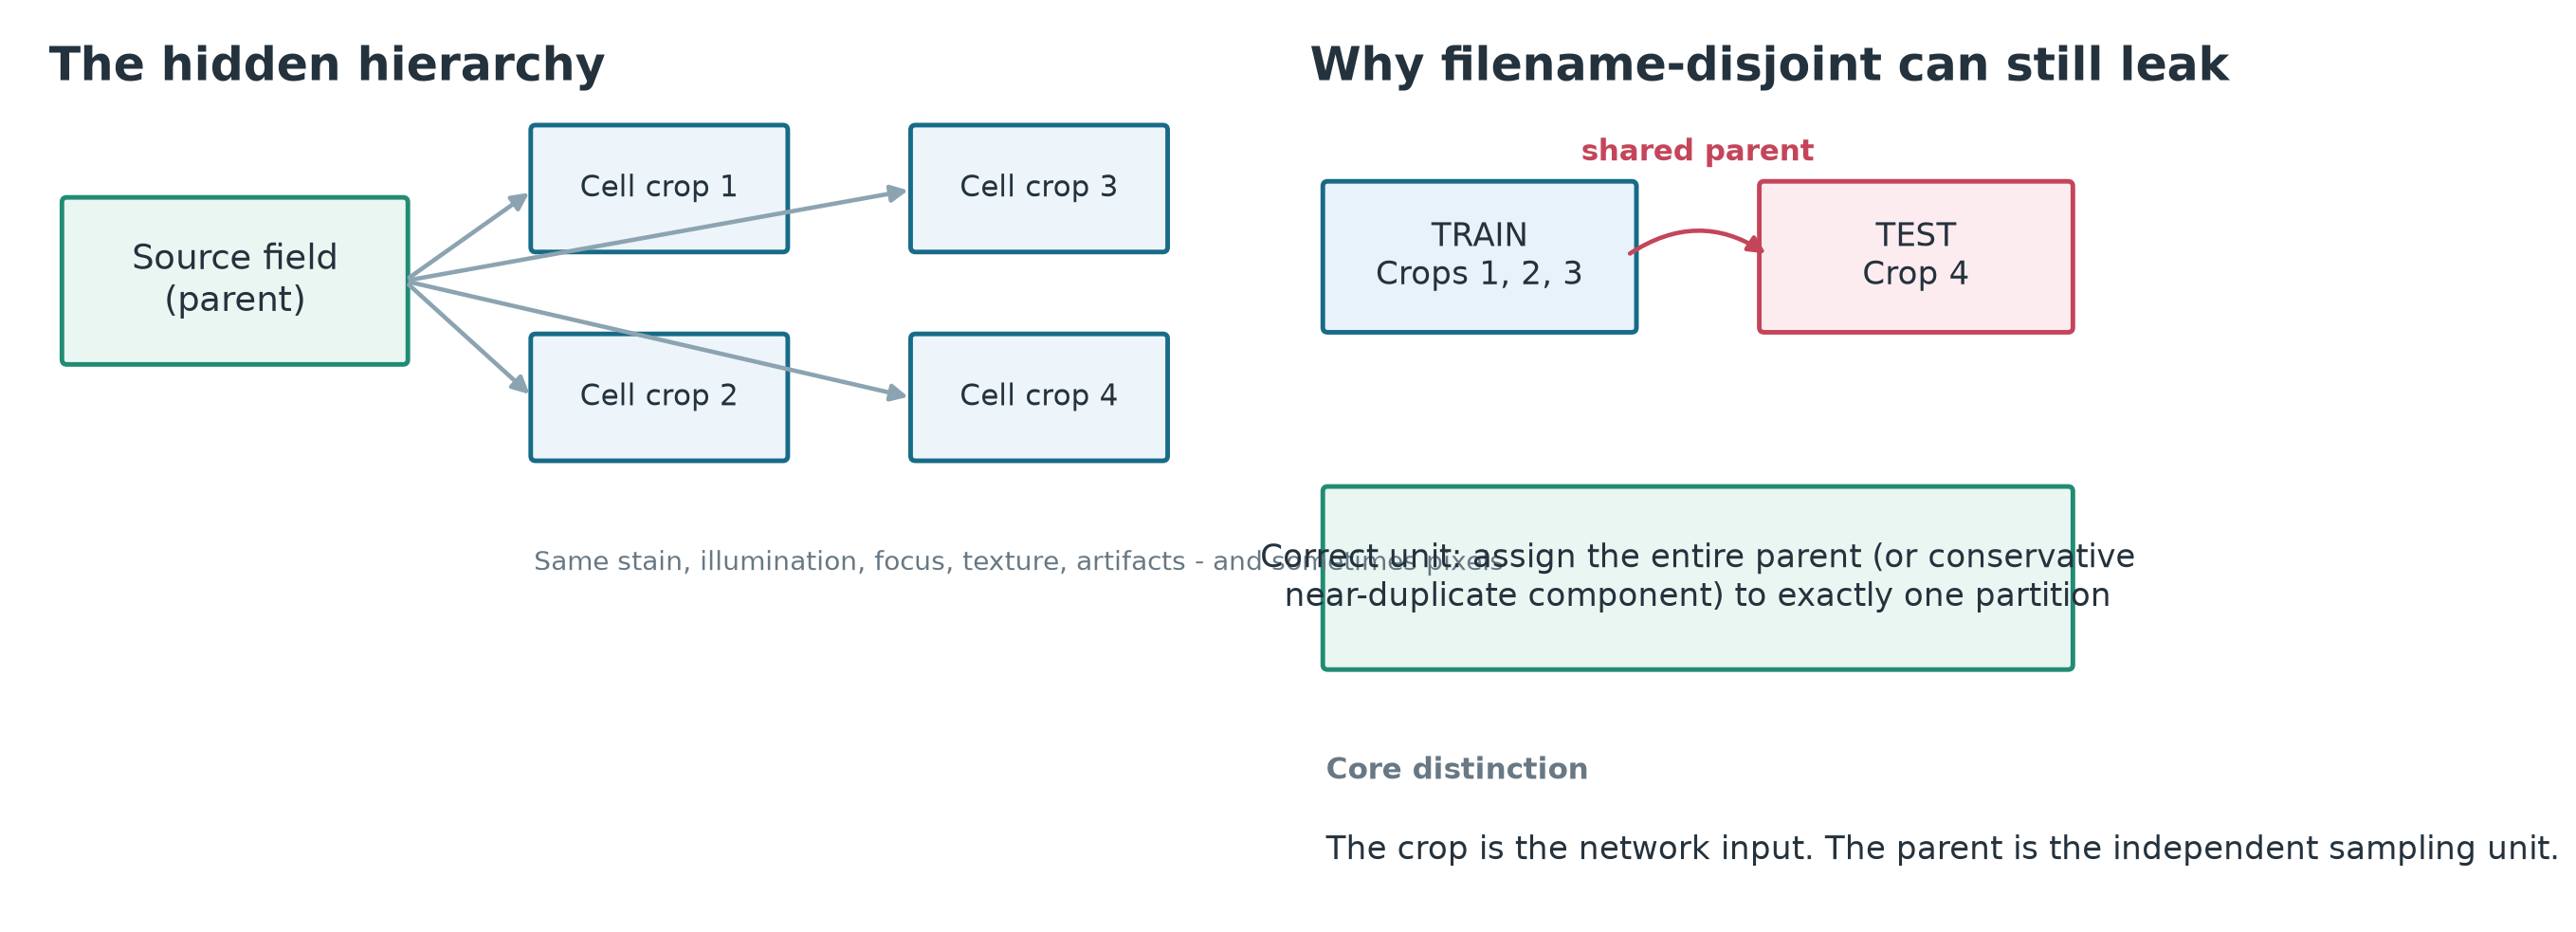
\includegraphics[width=0.92\textwidth]{hierarchy_and_leakage.png}
\vfill
{\Large\bfseries Snehasish Ghosh\textsuperscript{1}, Soham Mitra\textsuperscript{2}, Nibaran Das\textsuperscript{2}}\\[0.3cm]
{\normalsize
\textsuperscript{1}Indian Institute of Science, Bengaluru, India\quad
\textsuperscript{2}Jadavpur University, Kolkata, India}
\vfill
{\large Evidence through 20 October 2026 (Asia/Kolkata)\\[0.15cm]
\normalsize \RecAllModels\ trained models, 640 evaluation-only runs, \RecCommits\ commits, two registered studies}\\[0.5cm]
{\color{CytoBlue}\rule{\textwidth}{2.2pt}}
\end{titlepage}

\pagenumbering{roman}
\chapter*{About this record}
\addcontentsline{toc}{chapter}{About this record}

This is the complete record of the \cytofair{} project from its first registered commit on 22 August 2026 to
the end of the follow-up experiments on 20 October 2026. It is deliberately exhaustive. It keeps the original
Study~1 record intact as Part~II, and adds everything that happened afterwards: the review that turned Study~1's
weaknesses into a scaling roadmap, the separately preregistered Study~2, the engineering needed to run \RecAllTasks
GPU tasks on a shared host with a four-core CPU allowance, every registered result, the eight follow-up
hypotheses of Amendment~8, the bugs and setbacks, and what the project established, refuted, and left open.

\begin{keybox}{Evidence boundary}
Every number in Parts~I and III--VIII is generated from committed outputs: the registered analysis files in
\artifact{results/study2/analysis} and \artifact{results/study2/followup}, the exported run records in
\artifact{results/study2/run_records}, the power simulation, the provenance maps, and the git history. The
generators are \artifact{scripts/study2/paper_numbers.py}, \artifact{record/scripts/make_record_tables.py}, and
\artifact{record/scripts/make_record_figures.py}; no result is typed by hand. Part~II is the Study~1 record of 13
September 2026, carried over verbatim (labels prefixed so they cannot collide), and its numbers come from the Study~1
result files as they stood then.
\end{keybox}

\begin{warningbox}{What ``preregistered'' means here}
Study~2 and Amendment~8 were registered as commits in version control before any model whose result they govern was
trained, and the registration commit's hash is recorded inside every run record. That is strong internal evidence, but
the commits have not yet been pushed or deposited with a third party, so an outside reader cannot yet verify their
dates independently. Amendment~8 was written after Study~2's results were known and is reported as a registered
follow-up, not as part of Study~2.
\end{warningbox}

\section*{How the record is organised}

\begin{description}[leftmargin=2.2em,style=nextline]
\item[Part I, the lifecycle at a glance] One chapter with the whole story: timeline, every registered test and its
verdict, the hypothesis map, and the answers to ``what did we get out of it?''.
\item[Part II, Study 1] The frozen Study~1 record: motivation, provenance recovery, structural leakage, literal overlap,
the parent-identity probe, the SIPaKMeD and Cx22 rescoring, statistics, execution failures, verification, and release.
\item[Part III, from Study 1 to Study 2] The roadmap and our response to each item, Phase~0 checks, the Study~2
preregistration, power analysis, every design (splits, factorial, transplants, adversary, CRIC), the structural closed
forms, and the post hoc reanalysis of Study~1.
\item[Part IV, engineering and execution] The host, its constraints, the GPU-resident input path, determinism, the
trainer's artifact schema, the scheduler, failure handling, smoke tests, the execution timeline, compute, archiving,
and the complete log of errors and fixes.
\item[Part V, Study 2 results] H1 to H5 with every sensitivity analysis and secondary analysis, training curves,
calibration, confusion matrices, and per-architecture detail.
\item[Part VI, Amendment 8] The follow-up question, the eight registered hypotheses, their designs, the preparer bug
(Amendment~9), every result, and the mechanism by elimination.
\item[Part VII, synthesis] What was established, refuted, and left open; what worked and what did not; lessons;
threats to validity; recommendations; publication options; decisions only the authors can make.
\item[Part VIII, appendices] The Study~1 appendices, complete run ledgers for every Study~2 and follow-up run, variance
components, power grid, risk report, the full commit chronology, registration hashes, and a reproduction cookbook.
\end{description}

\section*{Reading paths}

\begin{itemize}[leftmargin=1.6em]
\item \emph{Ten minutes:} Part~I.
\item \emph{The science:} Part~I, Chapter~\ref{r:ch:roadmap}, Part~V, Part~VI, Chapter~\ref{r:ch:synthesis}.
\item \emph{Reproducing or extending the work:} Part~IV, Appendix~\ref{r:app:cookbook}, and the ledgers.
\item \emph{Writing a paper from it:} Chapter~\ref{r:ch:synthesis} (claims and their strength) and
Section~\ref{r:sec:publication}.
\end{itemize}

\section*{Conventions}

P1 is a stratified crop-level 80:20 split; P1-prime (P1$'$) a size-matched control; P2 a parent-disjoint split (field,
source image, or slide); P3 a parent-disjoint split after merging near-duplicate-linked parents. ``pp'' means percentage
points. Unless stated otherwise, intervals are 95\%, times are Asia/Kolkata (IST), and ``supported'' means a registered
test passed its registered criterion (adjusted $p<0.05$ with the predicted sign). In figures, crop-level (leaky) series
are orange, parent-level blue, and component-level aqua; leak models are orange and clean models blue.

\tableofcontents
\listoffigures
\listoftables
\clearpage
\pagenumbering{arabic}

\part{The Lifecycle at a Glance}

\chapter{The whole project on a few pages}
\label{r:ch:overview}

\section{The question}

Public cervical cytology benchmarks are released as cell crops, and most crops are cut from far fewer microscope
fields or slide images. When a benchmark is split at the crop level, crops from one field land on both sides of the
train--test boundary. Files are disjoint, but the test set shares stain, illumination, focus, background, and sometimes
literal pixels with training. The project asked three questions in order: \emph{is the structure there}, \emph{is the
shared parent recognisable}, and \emph{does it inflate reported performance}; and then a fourth: \emph{how do models use
it}.

\section{What happened, in order}

\begin{figure}[H]
\centering
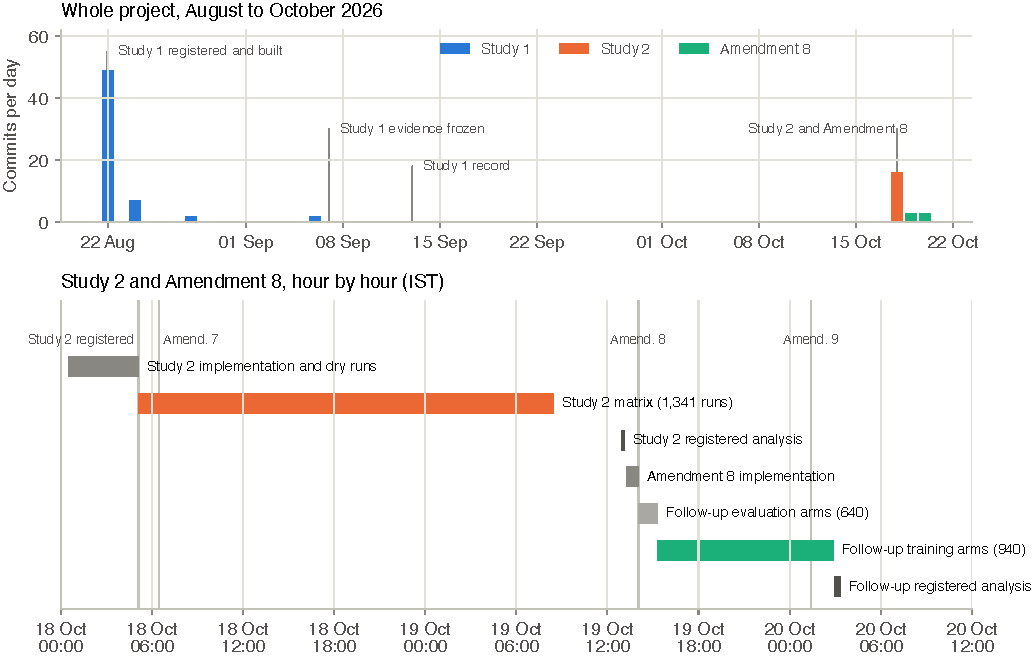
\includegraphics[width=\textwidth]{timeline.pdf}
\caption{The lifecycle. Top: commits per day across the project. Bottom: Study~2 and Amendment~8 hour by hour; every
span is measured from run records or commits.}
\label{r:fig:timeline}
\end{figure}

\begin{figure}[H]
\centering
\begin{adjustbox}{max width=\textwidth}
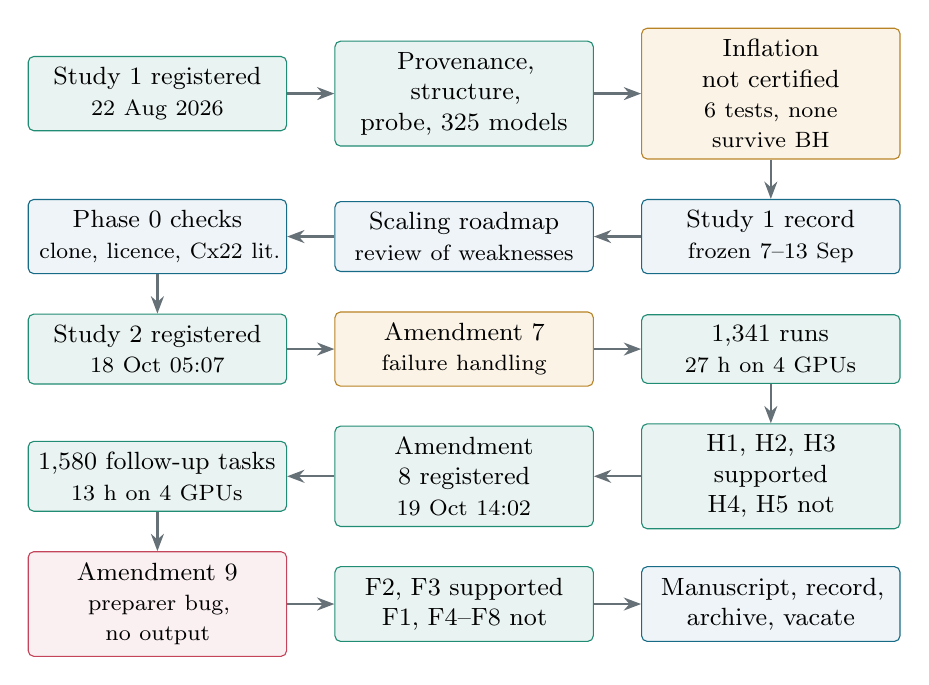
\begin{tikzpicture}[node distance=5mm and 6mm]
\node[done=30mm] (s1reg) {Study 1 registered\\\footnotesize 22 Aug 2026};
\node[done=30mm, right=of s1reg] (s1run) {Provenance, structure,\\probe, 325 models};
\node[gold=30mm, right=of s1run] (s1res) {Inflation not certified\\\footnotesize 6 tests, none survive BH};
\node[box=30mm, below=of s1res] (rec) {Study 1 record\\\footnotesize frozen 7--13 Sep};
\node[box=30mm, left=of rec] (road) {Scaling roadmap\\\footnotesize review of weaknesses};
\node[box=30mm, left=of road] (p0) {Phase 0 checks\\\footnotesize clone, licence, Cx22 lit.};
\node[done=30mm, below=of p0] (s2reg) {Study 2 registered\\\footnotesize 18 Oct 05:07};
\node[gold=30mm, right=of s2reg] (a7) {Amendment 7\\\footnotesize failure handling};
\node[done=30mm, right=of a7] (s2run) {1,341 runs\\\footnotesize 27 h on 4 GPUs};
\node[done=30mm, below=of s2run] (s2res) {H1, H2, H3 supported\\H4, H5 not};
\node[done=30mm, left=of s2res] (a8) {Amendment 8 registered\\\footnotesize 19 Oct 14:02};
\node[done=30mm, left=of a8] (frun) {1,580 follow-up tasks\\\footnotesize 13 h on 4 GPUs};
\node[bad=30mm, below=of frun] (a9) {Amendment 9\\\footnotesize preparer bug, no output};
\node[done=30mm, right=of a9] (fres) {F2, F3 supported\\F1, F4--F8 not};
\node[box=30mm, right=of fres] (paper) {Manuscript, record,\\archive, vacate};
\draw[flow] (s1reg) -- (s1run); \draw[flow] (s1run) -- (s1res); \draw[flow] (s1res) -- (rec);
\draw[flow] (rec) -- (road); \draw[flow] (road) -- (p0); \draw[flow] (p0) -- (s2reg);
\draw[flow] (s2reg) -- (a7); \draw[flow] (a7) -- (s2run); \draw[flow] (s2run) -- (s2res);
\draw[flow] (s2res) -- (a8); \draw[flow] (a8) -- (frun); \draw[flow] (frun) -- (a9);
\draw[flow] (a9) -- (fres); \draw[flow] (fres) -- (paper);
\end{tikzpicture}
\end{adjustbox}
\caption{The whole lifecycle as a sequence of registered decisions (green), amendments and setbacks (gold, red),
and reviews (blue). Every arrow is a commit in the repository; Appendix~\ref{r:app:git} lists all of them.}
\label{r:fig:lifecycle-flow}
\end{figure}


\begin{enumerate}[leftmargin=1.8em]
\item \textbf{Study 1 (22 August -- 13 September 2026).} The crop-to-parent hierarchy of four public datasets was
recovered with independent, fail-closed branches; random crop splitting placed a training parent behind 92.6\% of
SIPaKMeD and 99.97\% of CRIC test cells; more than half of SIPaKMeD test crops shared source pixels with a training
crop; a 424-way parent probe reached 109 times chance. Classifiers scored higher under crop-level splits for all six
architectures and all seven Cx22 segmentation models, but none of the per-architecture tests survived the registered
Benjamini--Hochberg correction. Part~II is that record.
\item \textbf{The roadmap (October 2026).} A review identified four weaknesses: one question asked six times, availability
not distinguished from use, leakage confounded with training diversity, and only one rescored benchmark. It proposed a
single mixed-model test sized by simulation, causal arms, more architectures and seeds, preregistration, and keeping
every per-sample artifact (Chapter~\ref{r:ch:roadmap}).
\item \textbf{Study 2 (18--19 October).} Registered at commit \texttt{\RegistrationCommit} (\RegistrationTime), before any
Study~2 model was trained: one primary test (H1) and a Holm family of four mechanism tests (H2--H5), \RecStudyTwoRuns\
runs over \RecStudyTwoWall\ hours on four GPUs. H1, H2, and H3 were supported; H4 and H5 were not.
\item \textbf{Amendment 8 (19--20 October).} Eight new hypotheses about \emph{how} the leak is used, registered at
\texttt{\FollowupCommit} (\FollowupTime) after the Study~2 analysis and before any follow-up run: \RecFollowTasks\ tasks
over \RecFollowWall\ hours. F2 and F3 were supported; F1 went the opposite way; F4--F8 were null.
\item \textbf{Amendment 9 (20 October, 01:25).} A labelling bug in the follow-up preparer halted the analysis before it
produced output; fixed and recorded before any affected estimate was seen.
\item \textbf{Close-out.} Manuscript (\artifact{paper/v2}), this record, 121~GB of outputs archived and verified on the
network home, and the node-local disk vacated.
\end{enumerate}

\section{Every registered test}

{\footnotesize
\setlength{\tabcolsep}{3.5pt}
\begin{longtable}{llrrrrl}
\caption{Every registered confirmatory test of Study 2 and Amendment 8. H1 is tested alone; H2--H5 and F1--F8 are separate Holm families. Units as in the text (pp; slopes in pp per pp).}\label{r:tab:alltests}\\
\toprule
 & Question & Estimate & 95\% CI & $p$ & Holm $p$ & Verdict \\
\midrule
\endfirsthead
\toprule
 & Question & Estimate & 95\% CI & $p$ & Holm $p$ & Verdict \\
\midrule
\endhead
\bottomrule
\endfoot
H1 & SIPaKMeD P1 $-$ P2 accuracy (primary) & 0.97 & 0.59 to 1.39 & $<$0.001 & alone & \supported \\
H2 & CRIC P1 $-$ P2 accuracy & 12.08 & 11.16 to 12.99 & $<$0.001 & $<$0.001 & \supported \\
H3 & 2C leakage at matched diversity & 1.73 & 0.95 to 2.51 & 0.006 & 0.02 & \supported \\
H4 & 2B own-context route & 0.42 & \textminus{}0.35 to 1.18 & 0.23 & 0.23 & \notsupported \\
H5 & 2A gap vs recoverability & 0.059 & \textminus{}0.007 to 0.125 & 0.08 & 0.16 & \notsupported \\
F1 & CRIC slide-context pull & \textminus{}4.29 & \textminus{}8.60 to \textminus{}1.37 & $<$0.001 & 0.001 & \notsupported \\
F2 & test-time stain transfer & 1.27 & 0.38 to 2.16 & 0.005 & 0.03 & \supported \\
F3 & leak with backgrounds masked & 1.86 & 1.42 to 2.30 & $<$0.001 & $<$0.001 & \supported \\
F4 & colour augmentation & \textminus{}0.23 & \textminus{}0.81 to 0.35 & 0.43 & 1.00 & \notsupported \\
F5 & LEACE erasure & \textminus{}0.01 & \textminus{}0.10 to 0.07 & 0.72 & 1.00 & \notsupported \\
F6 & stain normalisation & 0.02 & \textminus{}0.41 to 0.44 & 0.94 & 1.00 & \notsupported \\
F7 & probe-matched adversary & 0.000 & \textminus{}0.038 to 0.039 & 0.99 & 1.00 & \notsupported \\
F8 & pooled dose-response & 0.000 & \textminus{}0.005 to 0.005 & 0.93 & 1.00 & \notsupported \\
\end{longtable}
}


\begin{figure}[H]
\centering
\begin{adjustbox}{max width=\textwidth}
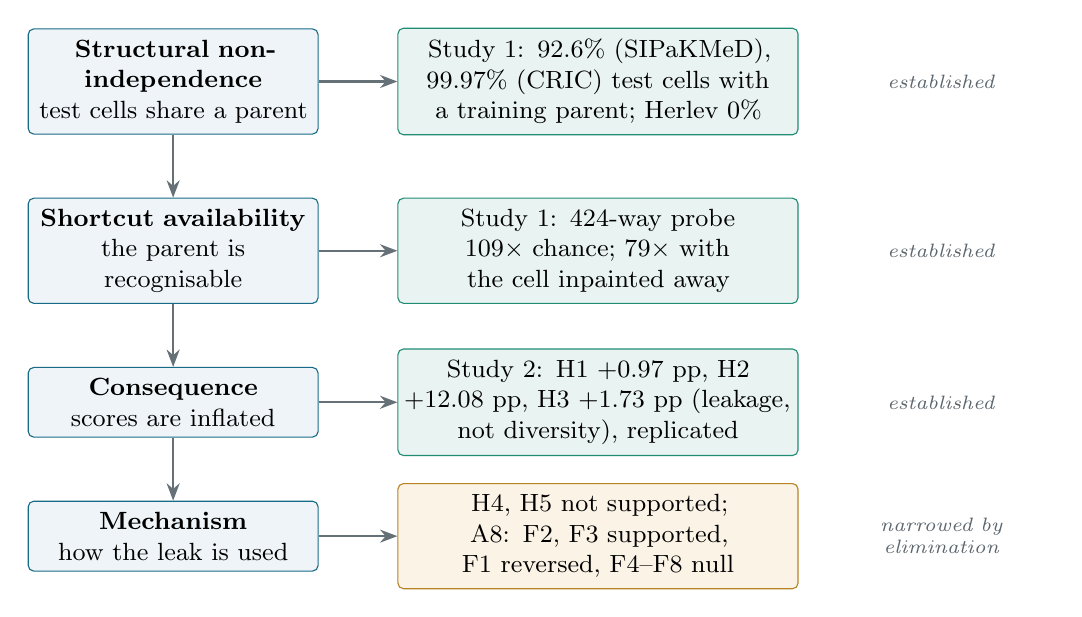
\begin{tikzpicture}[node distance=3mm and 5mm, every node/.style={font=\small}]
\node[box=34mm] (c1) {\textbf{Structural non-independence}\\test cells share a parent};
\node[box=34mm, below=8mm of c1] (c2) {\textbf{Shortcut availability}\\the parent is recognisable};
\node[box=34mm, below=8mm of c2] (c3) {\textbf{Consequence}\\scores are inflated};
\node[box=34mm, below=8mm of c3] (c4) {\textbf{Mechanism}\\how the leak is used};
\node[done=48mm, right=10mm of c1] (t1) {Study 1: 92.6\% (SIPaKMeD), 99.97\% (CRIC) test cells with a training parent; Herlev 0\%};
\node[done=48mm, right=10mm of c2] (t2) {Study 1: 424-way probe 109$\times$ chance; 79$\times$ with the cell inpainted away};
\node[done=48mm, right=10mm of c3] (t3) {Study 2: H1 +\HoneEst~pp, H2 +\HtwoEst~pp, H3 +\HthreeEst~pp (leakage, not diversity), replicated};
\node[gold=48mm, right=10mm of c4] (t4) {H4, H5 not supported; A8: F2, F3 supported, F1 reversed, F4--F8 null};
\node[note, right=4mm of t1, text width=26mm] {established};
\node[note, right=4mm of t2, text width=26mm] {established};
\node[note, right=4mm of t3, text width=26mm] {established};
\node[note, right=4mm of t4, text width=26mm] {narrowed by elimination};
\foreach \a/\b in {c1/t1,c2/t2,c3/t3,c4/t4} \draw[flow] (\a) -- (\b);
\draw[flow] (c1) -- (c2); \draw[flow] (c2) -- (c3); \draw[flow] (c3) -- (c4);
\end{tikzpicture}
\end{adjustbox}
\caption{The four claims the project separates, and the evidence each received. Study 1 established the first two;
Study 2 the third; Amendment 8 narrowed the fourth.}
\label{r:fig:hypothesis-map}
\end{figure}


\section{What we got out of it}

\begin{workedbox}{Established}
\begin{itemize}[leftmargin=1.4em]
\item Crop-level splitting inflates accuracy on SIPaKMeD by \HoneEst~pp (95\% CI \HoneBootLo--\HoneBootHi; all
twelve architectures positive) and on CRIC by \HtwoEst~pp; the parent-level error rate is \SipErrorRatio\ and
\CricErrorRatio\ times the crop-level one.
\item The inflation is leakage, not the extra training diversity crop-level splits bring: at matched crop and field
counts the leak effect is \HthreeEst~pp and the diversity effect \DivEst~pp; the leak effect replicated on fresh seeds
(\HthreeRepEst~pp).
\item The leak needs no background (F3: \FthreeEst~pp with every background masked) and is tied to the field's colour
rendering at test time (F2: stain transfer cuts it from \LeakUnderOriginal\ to \LeakUnderStain~pp).
\item Neither a linearly decodable field code nor Grad-CAM-visible attention carries it: erasing or adversarially
suppressing field identity cut probe recoverability by up to \RecoveryCutMax\% without moving the gap, and Grad-CAM maps
of leak and clean models were indistinguishable.
\end{itemize}
\end{workedbox}

\begin{warningbox}{Not supported, reversed, or open}
\begin{itemize}[leftmargin=1.4em]
\item H4 (a background context route) and H5 (the gap tracks gradient-reversal suppression) were not supported; the
ConvNeXt-T adversary was evaded.
\item F1 reversed: CRIC models were \emph{not} pulled toward the slide's majority label.
\item F4: strong colour augmentation did not prevent leakage, which qualifies F2.
\item Parents are not patients; one training recipe was used throughout; Study~2's registrations still need an external
timestamp.
\end{itemize}
\end{warningbox}

\begin{decisionbox}{The practical message}
Probes, saliency maps, background removal, and colour augmentation cannot certify that an evaluation is free of
hierarchical leakage. Only a split at the deepest released parent unit removes it, and the closed forms of
Chapter~\ref{r:ch:structure} predict which benchmarks are exposed before any model is trained.
\end{decisionbox}

\section{Numbers at a glance}

\begin{longtable}{p{0.55\textwidth}p{0.38\textwidth}}
\toprule
Quantity & Value \\
\midrule
Trained models (Study 1, Study 2, Amendment 8) & \RecAllModels\ (325 + \RecStudyTwoRuns\ + \RecFollowTrainRuns) \\
Evaluation-only runs on saved models (Amendment 8) & \RecFollowEvalRuns \\
Training epochs logged (Study 2 and Amendment 8) & \RecEpochs \\
GPU-hours, Study 2 / Amendment 8 & \RecGpuHoursStudyTwo\ / \RecGpuHoursFollow \\
Study 2 matrix wall clock & \RecStudyTwoWall\ h (\RecStudyTwoStart\ to \RecStudyTwoEnd) \\
Amendment 8 matrix wall clock & \RecFollowWall\ h (\RecFollowStart\ to \RecFollowEnd) \\
Failed tasks, retries, diverged runs & 0, 0, 0 \\
Smoke tests before registration & \RecSmokeRuns \\
Commits & \RecCommits \\
Registered confirmatory tests & 1 primary + 4 (Holm) + 8 (Holm) \\
\bottomrule
\end{longtable}

\part{Study 1: The Original Audit (August--September 2026)}

\chapter*{Reading Part II in context}
\addcontentsline{toc}{chapter}{Reading Part II in context}

Part~II is the Study~1 record exactly as it was compiled on 13 September 2026 from evidence frozen on 7 September. It is
reproduced verbatim so that the original claims, their strength, and their stated limitations remain on the record
unchanged. Three things happened afterwards that a reader of Part~II should keep in mind.

\begin{keybox}{What changed after Study 1}
\begin{itemize}[leftmargin=1.4em]
\item \textbf{The inflation question was re-asked and answered.} Study~1's six per-architecture tests could not certify an
accuracy inflation. Study~2 asked the question once, with a crossed mixed model sized by simulation and twenty new seeds,
and found \HoneEst~pp on SIPaKMeD (all twelve architectures positive) and \HtwoEst~pp on CRIC (Part~V). The six Study~1
architectures, re-run with fresh seeds, all moved in the same direction (Figure~\ref{r:fig:cross-study}).
\item \textbf{The ordering failure stands.} Study~1 registered that P3 $\leq$ P2 $\leq$ P1 and found it failed for four of
six architectures. Study~2's P2 $-$ P3 contrast was \PtwoPthreeEst~pp ($p=\PtwoPthreeP$): merging near-duplicate-linked
parents on top of parent-level splitting changes nothing, so the ordering failure reflects noise between two equivalent
protocols, not a defect of P3.
\item \textbf{Availability is not use.} Study~1 showed the parent fingerprint is learnable. Amendment~8 showed that the
fingerprint a probe can decode can be almost entirely removed without touching the inflation (Part~VI). Study~1's
warning that availability does not prove use was correct, and the distinction turned out to matter.
\end{itemize}
\end{keybox}

Where Part~II says that per-sample predictions and checkpoints were not retained, that applied to Study~1; every
Study~2 and Amendment~8 run kept per-crop logits, final weights, and probe-split features.

% Carried over verbatim from monograph/main.tex (Study 1 record, 13 Sep 2026).
\chapter{Study 1 record: status, scope, and abstract}\label{s1:ch:ch00_status_scope}


This is the long-form technical record of the \cytofair{} project. It is intentionally broader than the six-page conference paper. It explains why the project was started, how every analysis was designed, how the code represents the data, what was measured, what worked, what failed, what was changed during execution, what remains unverified, and what artifacts can be reused. The report is written from the repository state and frozen result files; it does not add a new experiment.

\begin{keybox}{Evidence boundary}
The quantitative claims in this document come from committed CSV, JSON, Parquet, source, and report artifacts in the repository. The experiment inventory contains 120 SIPaKMeD classification runs, 30 parent-identity probe runs, and 175 Cx22 segmentation runs: 325 completed neural-network runs in total. Structural analyses are additional deterministic or Monte Carlo computations, not neural runs. No post-hoc classifier confusion matrix or qualitative model prediction is invented, because the frozen classifier JSON files retain aggregate metrics and epoch histories but not per-sample predictions or checkpoints.
\end{keybox}

\begin{warningbox}{How to interpret ``leakage'' in this report}
Structural non-independence, literal pixel overlap, and a learnable parent fingerprint are demonstrated. These facts establish that a shortcut is available. They do \emph{not} prove that every cervical-classification model causally uses that shortcut, and the multiplicity-corrected classifier contrasts do not establish a universal accuracy-inflation effect. This distinction is maintained throughout the report.
\end{warningbox}

\begin{keybox}{Abstract of the Study 1 record (13 September 2026)}
Cervical-cell datasets are frequently released as crops, even when several crops came from one microscopic field or source image. A random crop split can therefore place sibling crops in both training and test sets, making file-level disjointness look like biological or acquisition-level independence. CytoFair recovers the hidden crop-to-parent hierarchy, validates it with fail-closed checks, measures structural and literal overlap, constructs parent- and component-disjoint splits, probes whether source identity remains learnable after transformations, and re-scores classification and segmentation models under matched protocols. The audit recovered all 4,049 SIPaKMeD crops, 1,320 Cx22 regions, 11,534 CRIC cells, and 917 Herlev cells. Under random splitting, 92.62\% of SIPaKMeD test crops, 85.23\% of Cx22 test regions, and 99.97\% of CRIC test cells had a parent in training, whereas Herlev correctly remained at zero. More than half of SIPaKMeD test crops shared literal source pixels with a training crop. A 424-way parent probe reached 25.73\% accuracy against 0.2358\% chance. All six SIPaKMeD classifier P1--P2 point estimates and all seven Cx22 segmentation estimates were positive, but no confirmatory contrast survived its preregistered Benjamini--Hochberg family. The project therefore supports a strong benchmark-construction conclusion---evaluate at the independent parent unit---while retaining a narrower and appropriately uncertain model-performance conclusion.
\end{keybox}

% Carried over verbatim from monograph/main.tex (Study 1 record, 13 Sep 2026).
\chapter{Executive overview}\label{s1:ch:ch01_executive_overview}

\section{The entire project in one page}

The initial problem was simple to state: \emph{when a benchmark calls every image file an independent example, is that file really the unit that was independently sampled?} In cervical cytology, the answer can be no. One microscope field can emit several cell crops. If those crops are split independently, their source field can appear on both sides of evaluation.

The project followed a staged answer:
\begin{enumerate}[leftmargin=2em]
  \item define the independent parent unit for four public datasets;
  \item recover exact crop-to-parent mappings, using independent recovery branches where the release permits them;
  \item refuse downstream analysis unless agreement, geometry, counts, and uniqueness pass;
  \item calculate how often random crop splitting separates siblings;
  \item detect literal pixel overlap and conservative cross-parent near-duplicate components;
  \item create four fixed protocols that isolate independence from training-set size;
  \item ask whether parent identity is visually learnable after removing candidate cues;
  \item re-run multiple classifier and segmentation families over five fixed seeds;
  \item use paired inference, effect sizes, bootstrap intervals, and declared BH families;
  \item preserve failed attempts and execution amendments rather than erasing them.
\end{enumerate}

\begin{figure}[H]
\centering
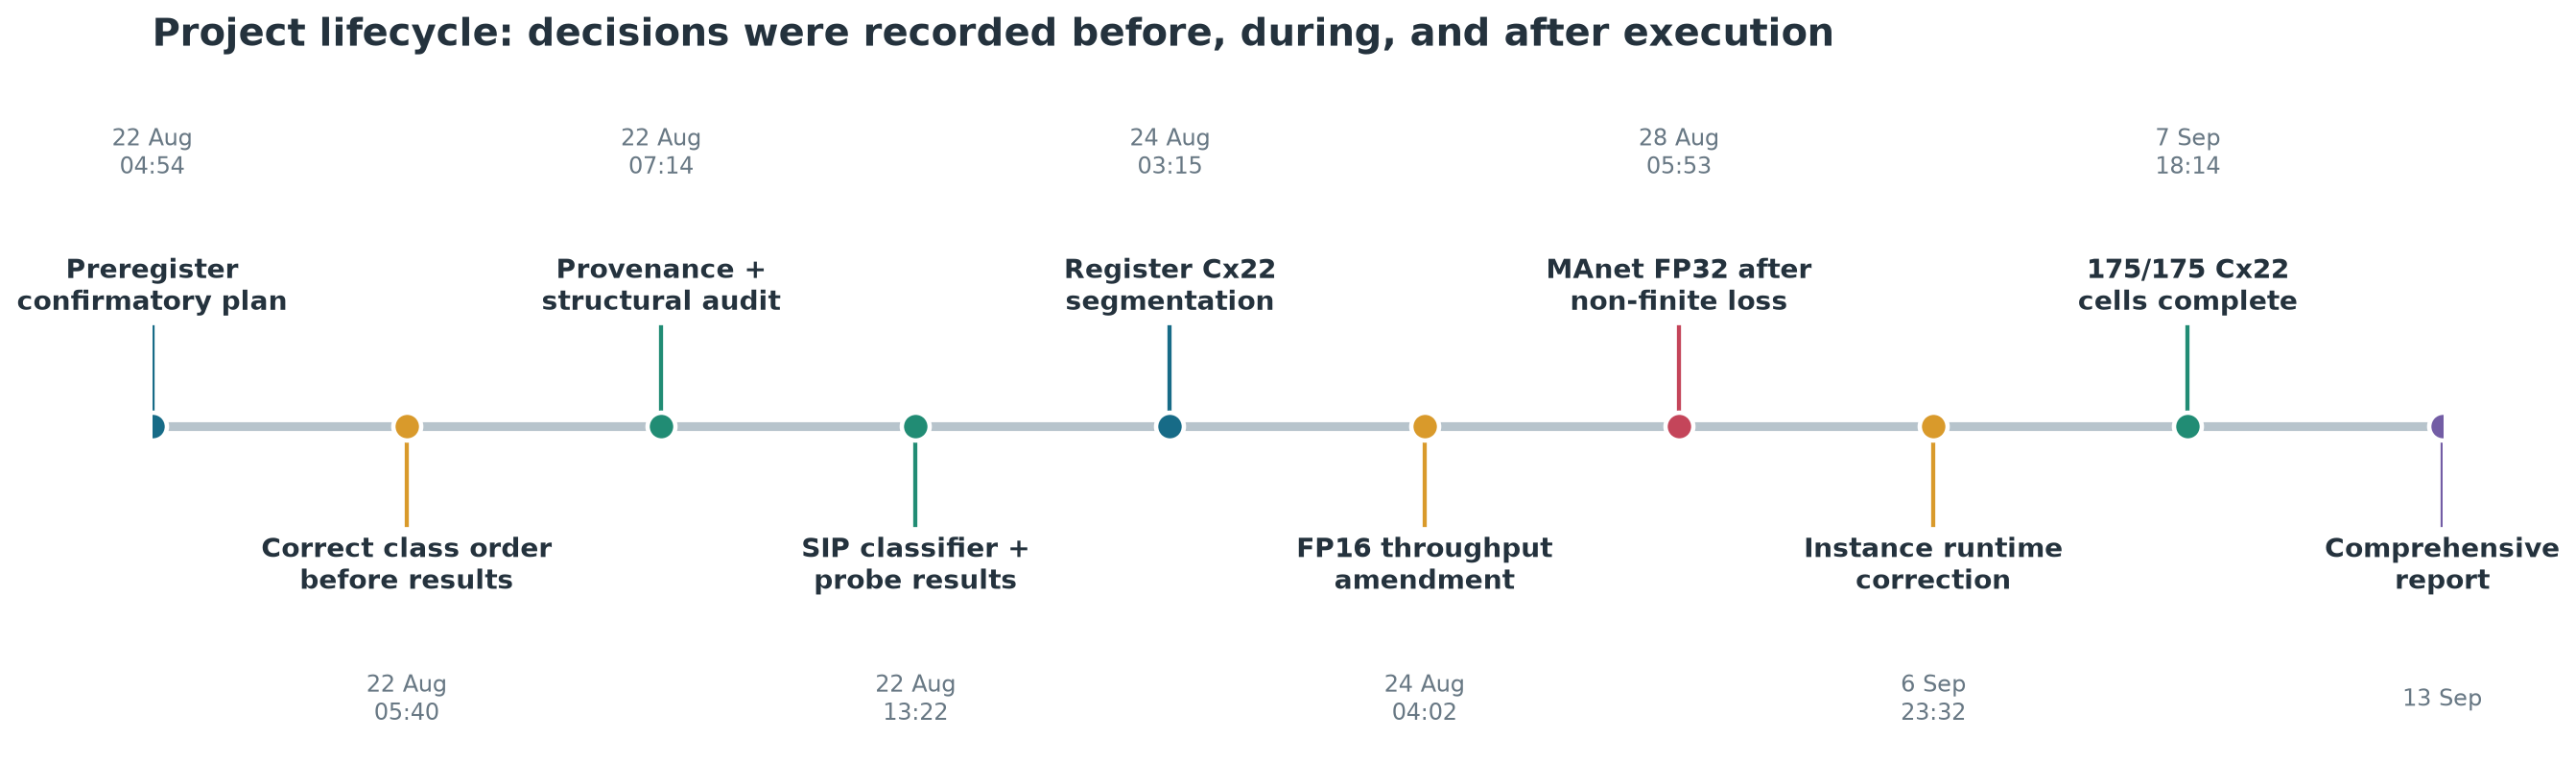
\includegraphics[width=\textwidth]{lifecycle_timeline.png}
\caption{The project lifecycle. Blue events register decisions, green events record completed evidence, gold events document execution-driven amendments, red records a numerical failure, and purple marks this report.}
\label{s1:fig:lifecycle}
\end{figure}

\section{Headline findings, without spin}

\begin{longtable}{p{0.22\textwidth}p{0.19\textwidth}p{0.51\textwidth}}
\caption{Headline conclusions and their correct strength.}\label{s1:tab:headline}\\
\toprule
Question & Answer & Evidence and boundary \\
\midrule
\endfirsthead
\toprule
Question & Answer & Evidence and boundary \\
\midrule
\endhead
\bottomrule
\endfoot
Can provenance be recovered? & Yes & SIPaKMeD branches agree on 4,049/4,049 crops; all boxes are contained; all dataset and class totals match. \\
Does random crop splitting share parents? & Yes & Mean P1 test-parent overlap is 92.62\% on SIPaKMeD, 85.23\% on Cx22, and 99.97\% on CRIC. \\
Does the negative control remain negative? & Yes & Herlev has one released cell per parent and returns exactly 0.00\% structural leakage for all seeds. \\
Are literal pixels shared? & Yes, in SIPaKMeD P1 & 52.62\% of test crops share at least one source pixel with a training crop; P2/P3 return zero. \\
Is source identity learnable? & Yes & A 424-way ResNet-18 reaches 25.73\% versus 0.2358\% chance; shuffled labels return 0.17\% and cover chance. \\
Is P1 accuracy universally inflated? & Not established & All six SIPaKMeD and all seven Cx22 P1--P2 means are positive, but no contrast survives BH correction. \\
Does stronger grouping always lower score? & No & SIPaKMeD's registered P3 $\leq$ P2 $\leq$ P1 model ordering fails for four of six architectures. The failure is retained. \\
Is Cx22's official split defective? & No such claim & The authors' Multi-Train/Multi-Test parent sets are disjoint. The pooled stress test asks what happens under a different downstream reuse pattern. \\
Is the release fully ready? & Not yet & The clean-clone/virgin-host evidence, lab-paper crosswalk, and independent Figure-1 reader gate remain pending. \\
\end{longtable}

% Carried over verbatim from monograph/main.tex (Study 1 record, 13 Sep 2026).
\chapter{Motivation and problem formulation}\label{s1:ch:ch02_motivation_and_problem_formulation}

\section{Why cervical cytology makes independence important}

Cervical cancer caused an estimated 660,000 new cases and 350,000 deaths worldwide in 2022~\cite{who2025hpv}. Cytology screening is a high-volume recognition problem: a small number of clinically important abnormal cells must be found among many plausible normal cells. Automation is attractive because it can help direct expert attention, but only if reported generalization represents genuinely unseen biological or acquisition units.

Modern cervical-cell classifiers report very high crop-level scores. DeepPap reported 98.3\% on Herlev~\cite{zhang2017deeppap}; DeepCervix reported 99.14\% on SIPaKMeD~\cite{rahaman2021deepcervix}; and a knowledge-distillation system reported 98.52\% on SIPaKMeD~\cite{gao2022knowledge}. These achievements motivated a basic audit question that is logically prior to choosing a stronger network: \emph{what population unit does the test set represent?}

\section{Observation, parent, and evaluation unit}

Let $x_i$ be a released image observation and let $g(x_i)=p_j$ map it to the acquisition unit that generated it. In this project:
\begin{itemize}
  \item $x_i$ is a SIPaKMeD cell crop and $p_j$ is a cluster field;
  \item $x_i$ is a Cx22 generated region and $p_j$ is a CCEDD source image;
  \item $x_i$ is a CRIC annotated cell and $p_j$ is its source smear image;
  \item $x_i$ is a Herlev single-cell image and is also its own parent.
\end{itemize}

The crucial idea is that the \emph{model input} and the \emph{independent sampling unit} need not be the same object. A network consumes $x_i$, but the statistical independence boundary may be $p_j$.

\begin{figure}[H]
\centering
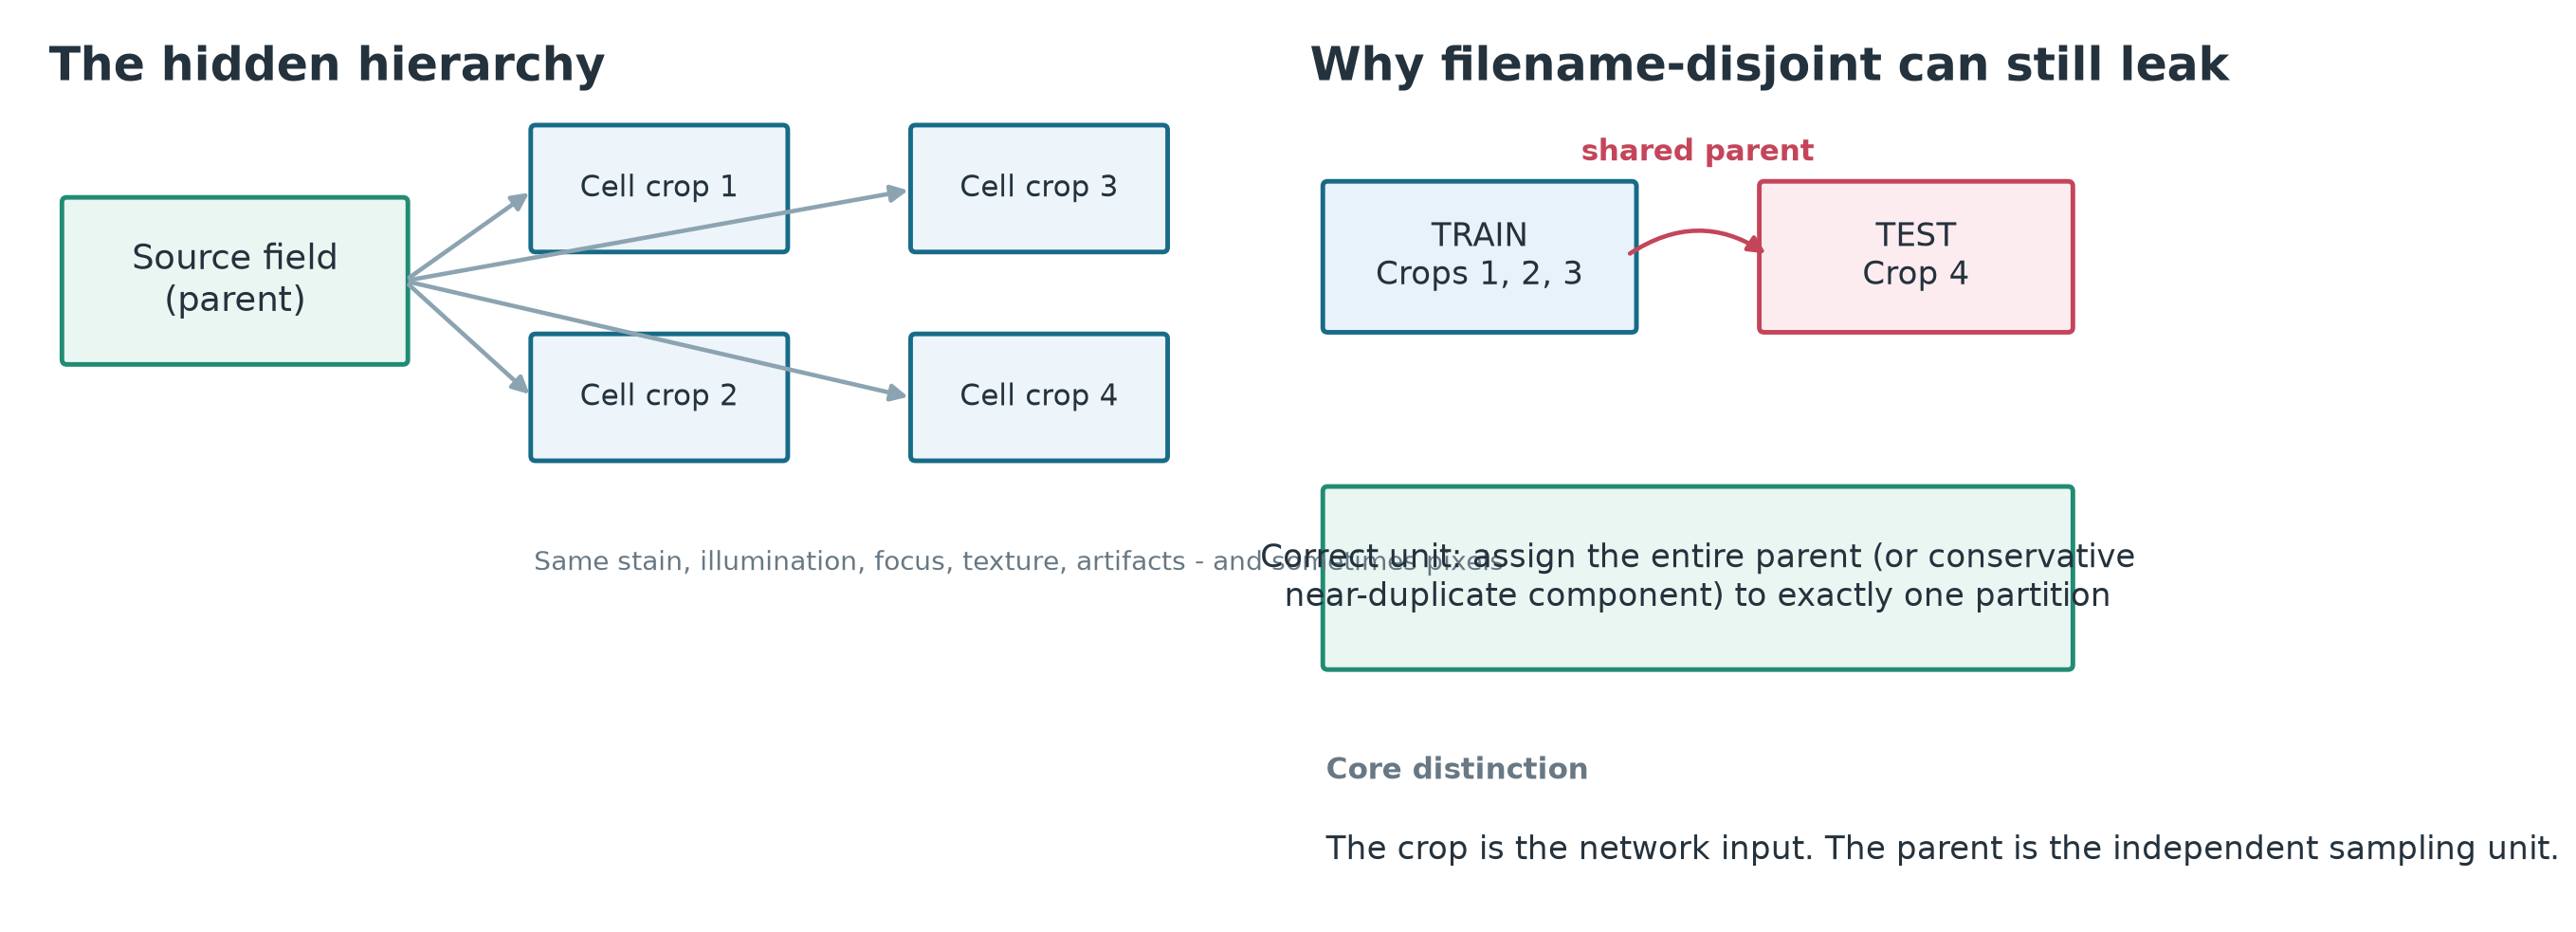
\includegraphics[width=\textwidth]{hierarchy_and_leakage.png}
\caption{The hidden hierarchy and the central failure mode. Several file-disjoint crops can share a parent field, source-specific nuisance factors, or literal source pixels.}
\label{s1:fig:hierarchy}
\end{figure}

\section{Three different claims that must not be conflated}

\begin{keybox}{Claim 1: structural non-independence}
Some parents contribute observations to both train and test. This can be established exactly from provenance and split assignments. It requires no model.
\end{keybox}

\begin{keybox}{Claim 2: shortcut availability}
A model can identify the source parent from held-out sibling crops at greater-than-chance accuracy. This shows that parent information survives in the released input. It does not yet show that a disease or morphology classifier uses it.
\end{keybox}

\begin{keybox}{Claim 3: downstream score inflation}
A crop-level protocol produces a larger score than a parent-disjoint protocol under matched models, seeds, and sample sizes. This is an empirical paired comparison. It needs uncertainty, multiplicity correction, and careful interpretation.
\end{keybox}

The project obtains strong evidence for Claims 1 and 2. For Claim 3, point estimates are directionally consistent across every tested architecture, but the confirmatory families do not cross the multiplicity-adjusted threshold. The report therefore never upgrades ``available shortcut'' into ``proven universal causal inflation.''

\section{Relationship to leakage and duplicate audits}

Duplicate-aware evaluation has been studied in general vision: ciFAIR removed near-duplicate CIFAR test counterparts~\cite{barz2020cifair}; license-plate work re-evaluated models under duplicate-free splits~\cite{laroca2023lpr}; and medical-image re-identification demonstrated that patient identity can be highly learnable~\cite{packhauser2022reidentification}. Kapoor and Narayanan place these problems in a broader taxonomy of data leakage and reproducibility failures~\cite{kapoor2023leakage}. CytoFair's distinctive concern is an exact cervical-cytology source hierarchy: sibling crops can be non-independent without being duplicate files.

% Carried over verbatim from monograph/main.tex (Study 1 record, 13 Sep 2026).
\chapter{Preregistration and analysis governance}\label{s1:ch:ch03_preregistration_and_analysis_governance}

\section{Why the plan was committed first}

The original preregistration was committed at 04:54:10 IST on 22 August 2026 (commit \artifact{67e8ded}). The first result commit was recorded at 13:22:42 IST that day (commit \artifact{1c2da7f}). The plan therefore predates the committed results. This matters because a five-seed matrix contains many possible comparisons; fixing endpoints, seeds, exclusions, and multiplicity families before seeing scores reduces analyst degrees of freedom.

The fixed confirmatory seeds were $17,29,43,71,101$. Five additional robustness seeds were named but were not needed for the reported confirmatory summaries and were not substituted for any unfavorable seed. Every protocol-architecture cell had to contain at least five valid paired runs before inferential output could be emitted.

\section{Registered endpoints}

The structural endpoints were (i) fraction of parents straddling train and test and (ii) fraction of test observations whose parent appears in training. The mechanistic endpoint was 424-way parent-identification accuracy. The SIPaKMeD model endpoint was test accuracy; macro-F1 and balanced accuracy were concordance metrics. For Cx22 semantic segmentation, the primary endpoint was mean per-image cytoplasm/nucleus Dice. For Cx22 instance segmentation, the primary endpoint was per-image mean ground-truth-instance Dice after maximum-weight matching, with unmatched targets assigned zero.

\section{Amendments: what changed and why}

\begin{longtable}{p{0.10\textwidth}p{0.16\textwidth}p{0.26\textwidth}p{0.34\textwidth}}
\caption{Registered amendments and their evidential status.}\label{s1:tab:amendments}\\
\toprule
Date & Amendment & Trigger & Why it did not select a favorable result \\
\midrule
\endfirsthead
\toprule
Date & Amendment & Trigger & Why it did not select a favorable result \\
\midrule
\endhead
\bottomrule
\endfoot
22 Aug & SIPaKMeD class order & The integrity gate exposed a transcription swap between Metaplastic and Dyskeratotic. & Corrected before any SIPaKMeD result; numeric target vector 126/108/238/271/223 did not change. \\
24 Aug & Cx22 segmentation extension & Structural Cx22 results motivated a separately scoped model rescore. & Registered before any Cx22 model was trained; official split retained as descriptive control. \\
24 Aug & FP16 execution & Full FP32 preflight left three A6000s under-used and made one U-Net epoch exceed 4.5 minutes. & Changed numerical execution before an epoch emitted a result; models, splits, seeds, endpoints, and epoch count stayed fixed. \\
28 Aug & MAnet in FP32 & The first MAnet P1 seed-17 attempts produced non-finite losses at epochs 23 and 24. & No completed MAnet result existed. All MAnet cells restarted from their fixed seeds rather than selecting a pre-divergence checkpoint. \\
28 Aug & Deterministic CUDA workspace & Startup warnings showed deterministic matrix multiplication required \artifact{CUBLAS_WORKSPACE_CONFIG=:4096:8}. & Frozen before a corrected MAnet or instance epoch existed; applied to all remaining cells. \\
6 Sep & Instance runtime correction & Evaluation every epoch, CPU mask matching, and frequent network checkpoint writes caused severe under-utilization. & The registered endpoint was final epoch. Intermediate test inference was removed, exact binary intersections moved to GPU, and recovery checkpoints became five-epoch; final computation stayed identical. \\
\end{longtable}

\begin{decisionbox}{A useful demotivation}
The project began with the possibility of a large, architecture-general accuracy correction. The statistics did not support that broad claim. Instead of hiding this, the project narrowed its claim: the benchmark hierarchy is demonstrably non-independent, the source signal is demonstrably learnable, and parent grouping removes the measured sharing. The size of downstream score inflation remains model- and task-dependent.
\end{decisionbox}

% Carried over verbatim from monograph/main.tex (Study 1 record, 13 Sep 2026).
\chapter{Datasets and the hidden hierarchy}\label{s1:ch:ch04_datasets_and_the_hidden_hierarchy}

\section{Overview}

\begin{table}[H]
\centering
\caption{Audited datasets and independent units.}
\label{s1:tab:datasets}
\begin{tabularx}{\textwidth}{lrrrXX}
\toprule
Dataset & Observations & Parents & Mean/parent & Released task & Parent definition \\
\midrule
SIPaKMeD & 4,049 & 966 & 4.19 & 5-class classification & cluster field \\
Cx22 & 1,320 & 514 & 2.57 & semantic/instance segmentation & CCEDD source image \\
CRIC & 11,534 & 400 & 28.84 & cytology classification resource & source smear image \\
Herlev & 917 & 917 & 1.00 & 7-class single-cell classification & released cell image \\
\bottomrule
\end{tabularx}
\end{table}

\begin{figure}[H]
\centering
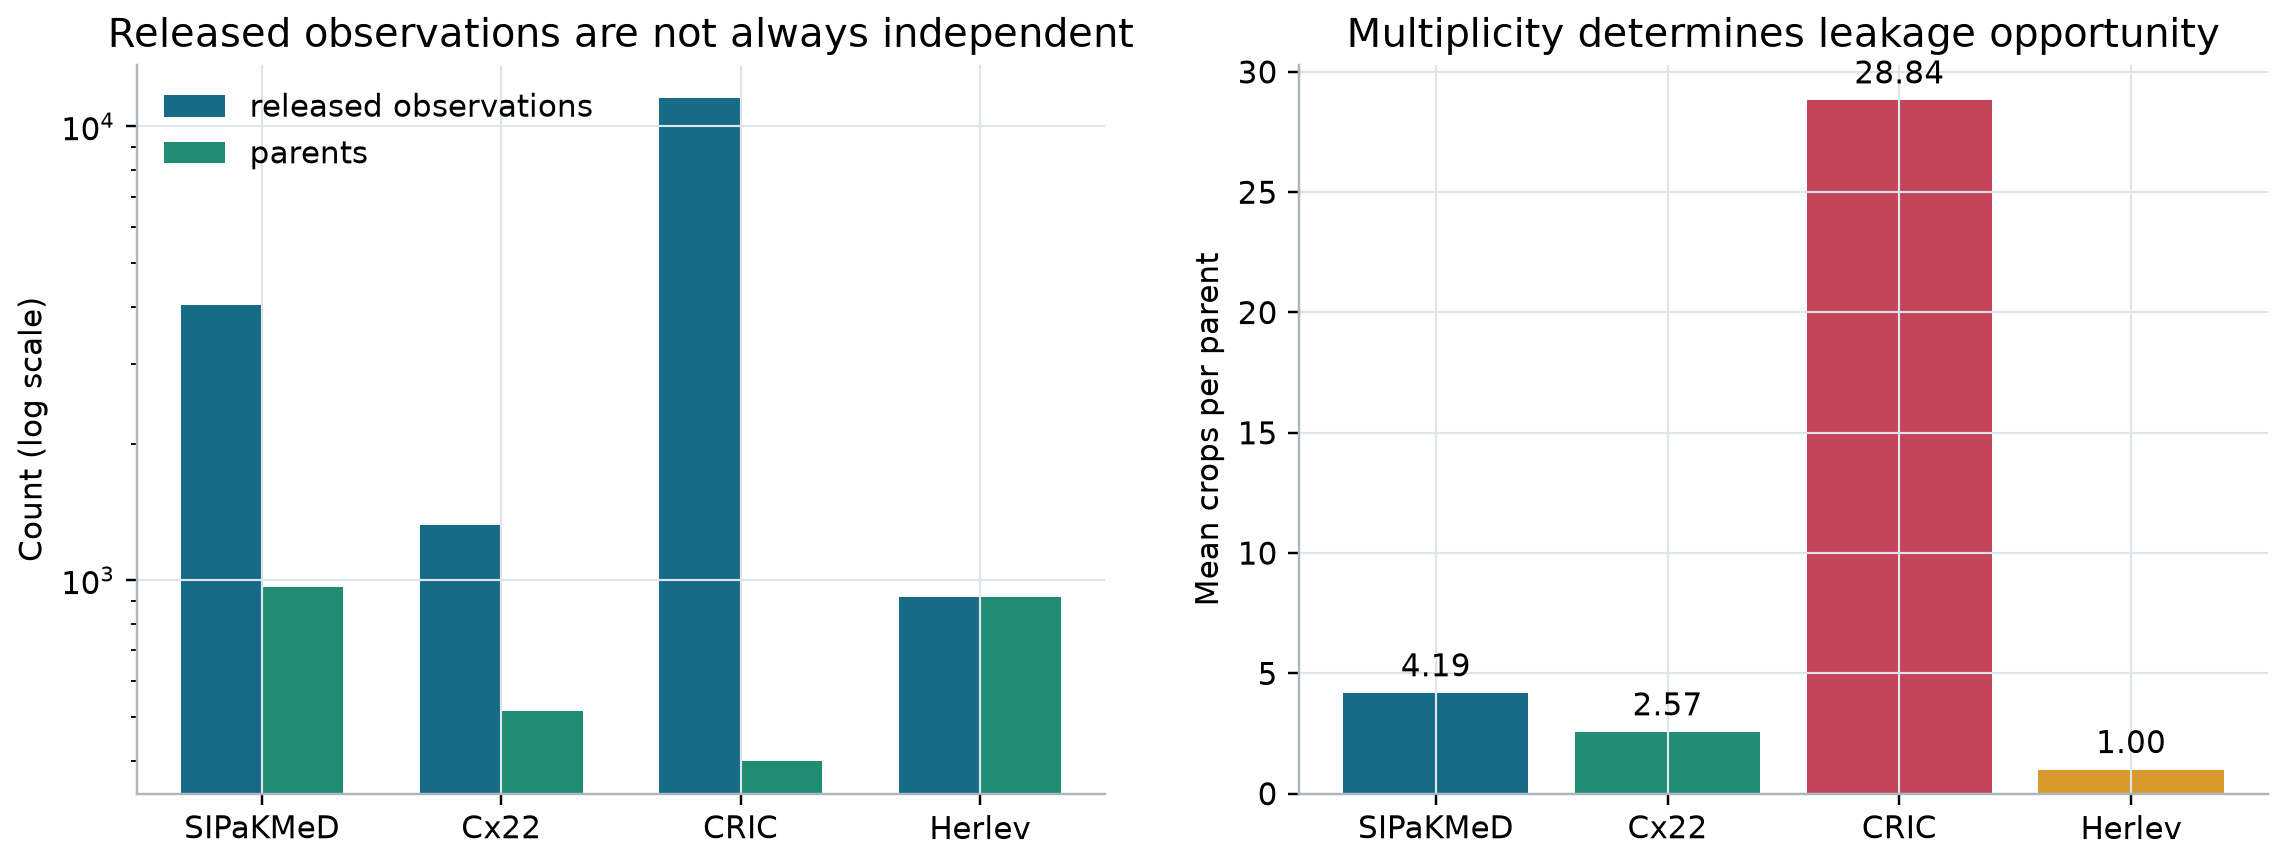
\includegraphics[width=\textwidth]{dataset_scale.png}
\caption{Dataset scale and mean parent multiplicity. The log-scale left panel prevents CRIC's 11,534 observations from visually erasing the smaller datasets.}
\label{s1:fig:dataset-scale}
\end{figure}

\begin{figure}[H]
\centering
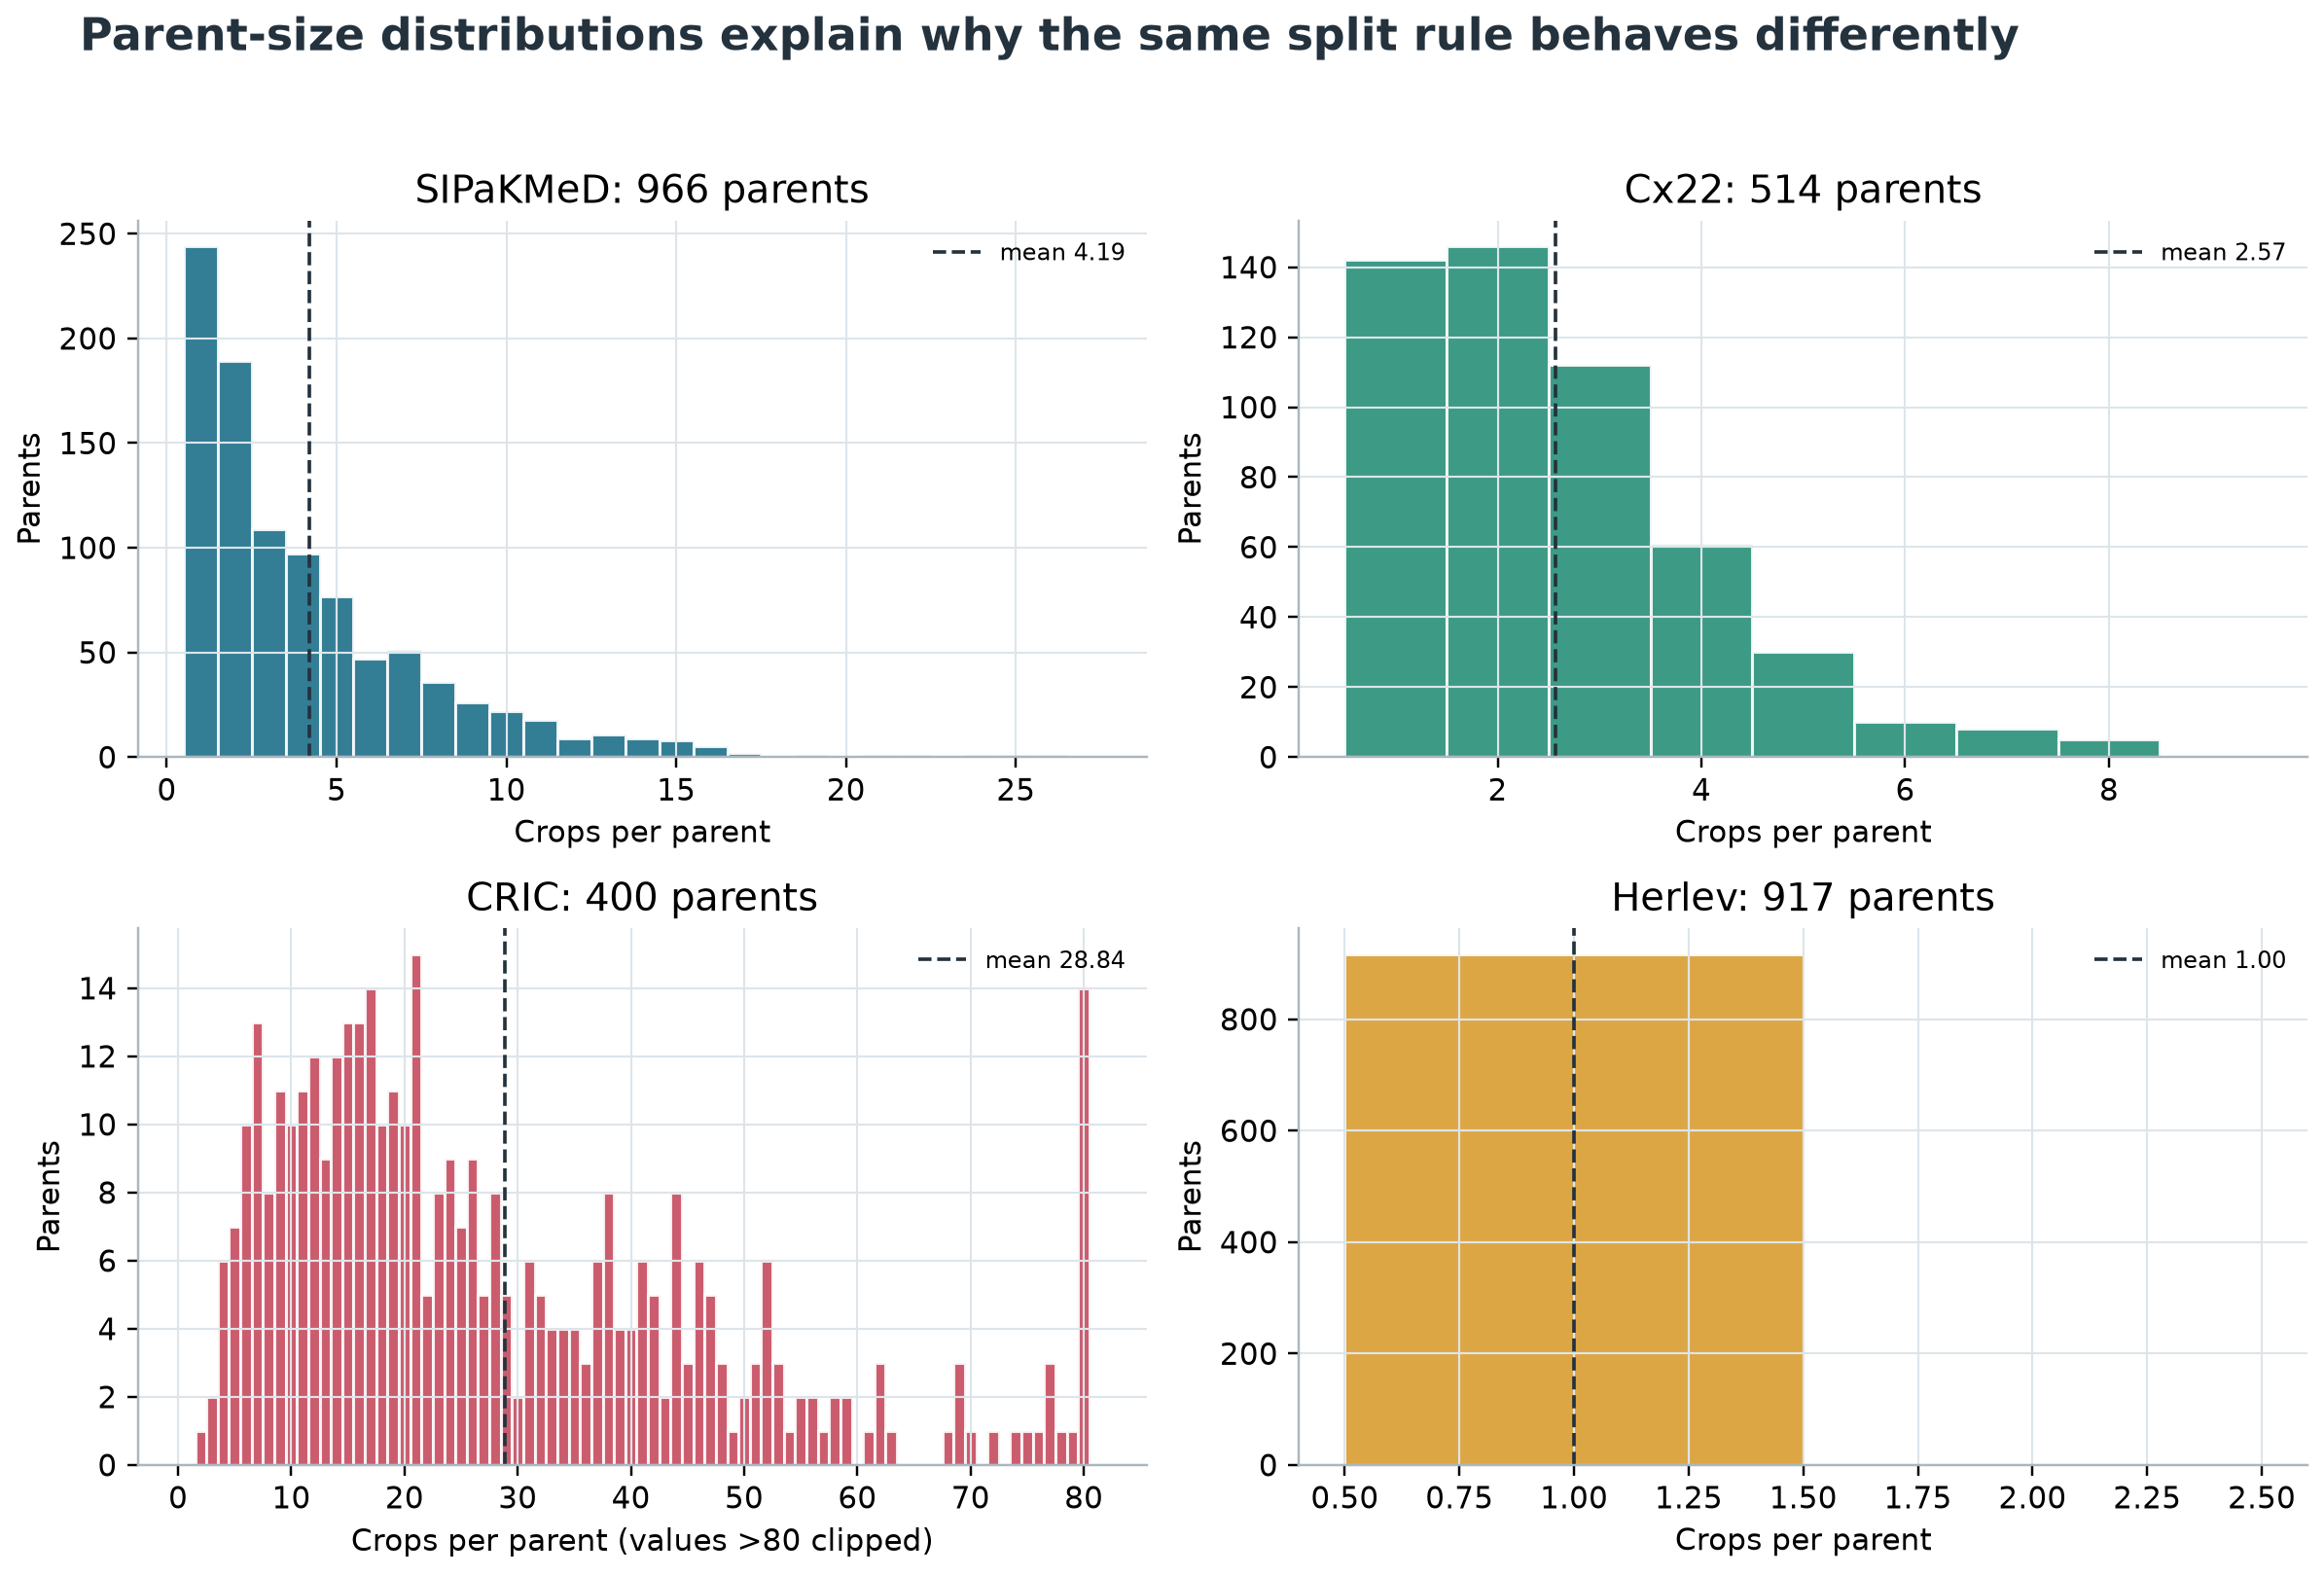
\includegraphics[width=\textwidth]{parent_size_distributions.png}
\caption{Complete parent-size distributions recovered from the Parquet maps. High multiplicity drives the probability that random crop splitting places a parent in both arms.}
\label{s1:fig:parent-distributions}
\end{figure}

\section{SIPaKMeD}

SIPaKMeD contains 4,049 isolated cell images derived from 966 cluster fields~\cite{plissiti2018sipakmed}. The released hierarchy is unusually valuable for an audit: full fields and a \artifact{CROPPED} directory coexist, and crop filenames encode the field identifier. The project uses the cluster field---not the crop file---as the parent.

\begin{table}[H]
\centering
\caption{Independently reconstructed SIPaKMeD class totals in release order.}
\label{s1:tab:sip-classes}
\begin{tabular}{lrrr}
\toprule
Class & Crops & Parents & Crops/parent \\
\midrule
Superficial--Intermediate & 831 & 126 & 6.60 \\
Parabasal & 787 & 108 & 7.29 \\
Koilocytotic & 825 & 238 & 3.47 \\
Metaplastic & 793 & 271 & 2.93 \\
Dyskeratotic & 813 & 223 & 3.65 \\
\midrule
Total & 4,049 & 966 & 4.19 \\
\bottomrule
\end{tabular}
\end{table}

The class order deserves explicit mention because the original planning text swapped the final two names even though its numerical vector was right. The integrity gate exposed that inconsistency, and Amendment 1 corrected it before results existed. This is an example of a check preventing a quiet metadata error.

\section{Cx22 and CCEDD}

Cx22 provides 1,320 generated regions and instance labels, drawing source images from CCEDD~\cite{liu2022cx22}. Three released subsets are involved: Multi-Train, Multi-Test, and Pair. The parent is the named CCEDD source image. Generator metadata provide source name and requested ROI coordinates; the authors' MATLAB generator defines how a source rectangle is clipped, resized, and pasted into a 512-by-512 white canvas.

The official Multi-Train and Multi-Test arms have zero shared parents. Pair is separately released and shares 55 parents with Multi-Test (Jaccard 0.126) and 233 with Multi-Train (Jaccard 0.475). The later model matrix pools all 1,320 observations only as a preregistered stress test of downstream reuse. It is not an accusation that the official authors used a leaking split.

\begin{figure}[H]
\centering
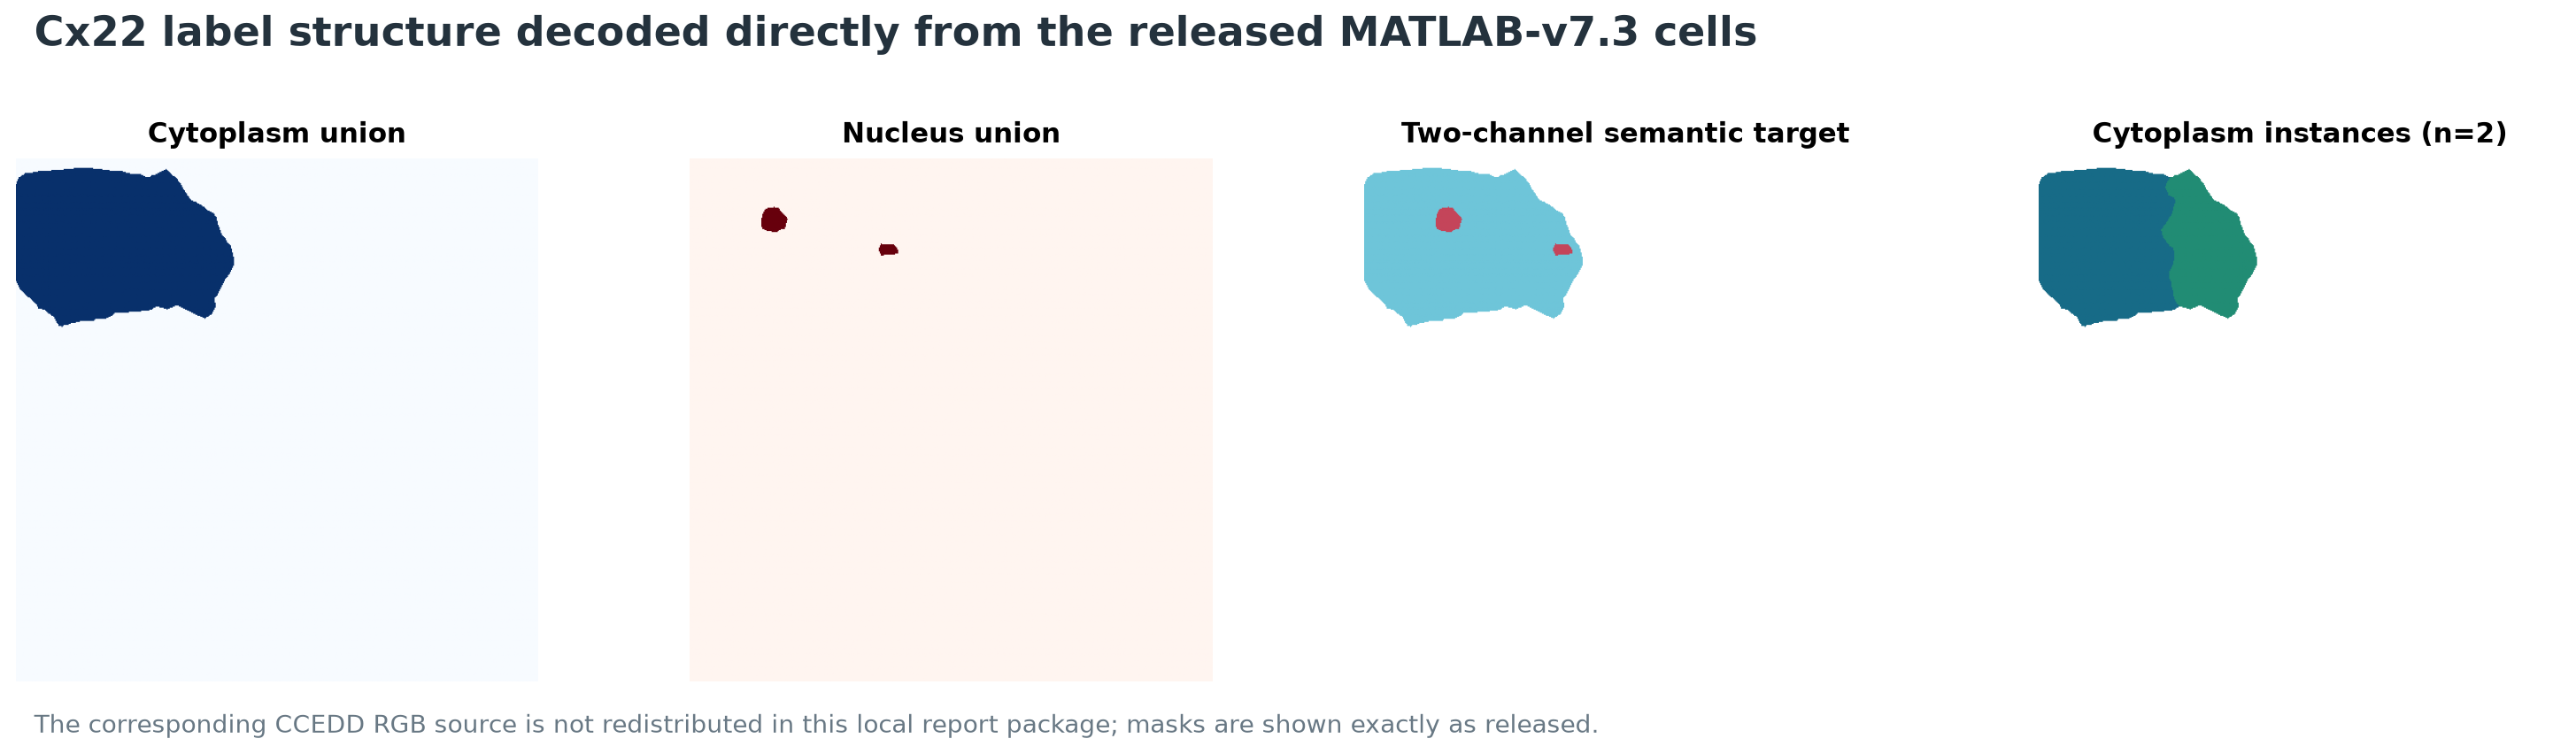
\includegraphics[width=\textwidth]{cx22_label_structure.png}
\caption{One released Cx22 Pair target decoded from the MATLAB-v7.3 structures. Cytoplasm and nucleus unions define two non-exclusive semantic channels; individual cytoplasm masks define the instance task. The CCEDD RGB source is not redistributed in this report.}
\label{s1:fig:cx22-labels}
\end{figure}

\section{CRIC}

CRIC contains 11,534 classified cells associated with 400 source images~\cite{rezende2021cric}. The released classification table supplies source identity and cell coordinates, which makes source-level grouping deterministic. A reliable patient identifier is not present in the released table, so the project does not claim patient-disjoint evaluation. This matters: source-image grouping is stronger than crop grouping but can still be weaker than patient grouping.

\section{Herlev as a structural negative control}

Herlev contains 917 released single-cell images~\cite{jantzen2005pap}. Under the project's declared data unit, each image is one observation and one parent. It therefore has no multi-observation parent structure and must return exactly zero parent straddling. If Herlev showed a nonzero structural effect, the implementation would be wrong. The control passed for all five seeds.

\section{Data-use constraints}

The repository publishes identifiers, coordinates, hashes, split assignments, code, and derived statistics. It does not redistribute raw images. Cx22/CCEDD material is restricted to non-commercial research/education in the declared source manifest, and CCEDD redistribution is prohibited. CRIC and the local Herlev repackaging are declared CC BY 4.0. SIPaKMeD's source notes require citation and experimental use. The complete URL/checksum/terms ledger appears in \cref{s1:tab:data-sources}.

% Carried over verbatim from monograph/main.tex (Study 1 record, 13 Sep 2026).
\chapter{System architecture and fail-closed philosophy}\label{s1:ch:ch05_system_architecture_and_fail_closed_phil}

\section{Pipeline}

\begin{figure}[H]
\centering
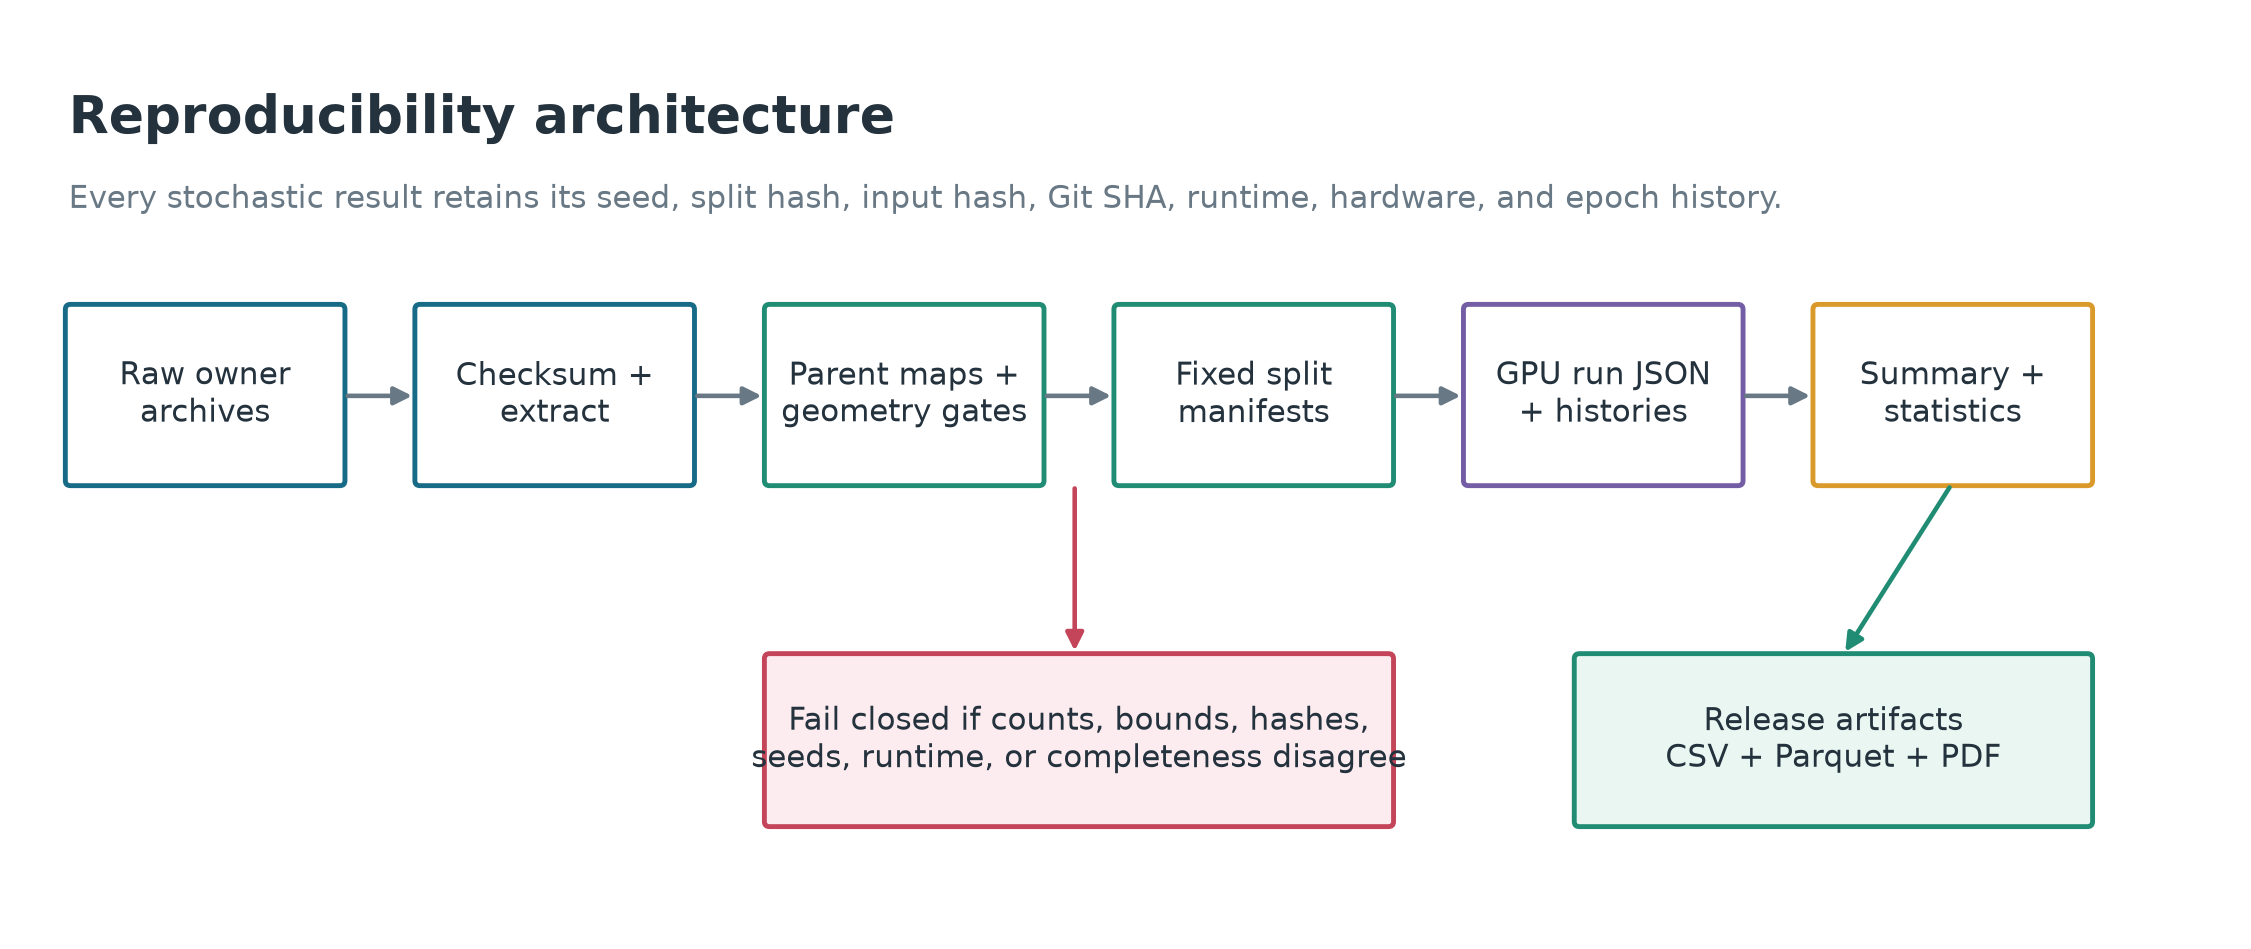
\includegraphics[width=\textwidth]{reproducibility_pipeline.png}
\caption{Reproducibility architecture. Deterministic provenance and split artifacts gate the stochastic GPU experiments, and every final result carries the hashes needed to reconnect it to its inputs.}
\label{s1:fig:repro-pipeline}
\end{figure}

The system deliberately separates three artifact layers:
\begin{enumerate}[leftmargin=2em]
  \item \textbf{Canonical identity:} exact or released parent IDs used to construct splits.
  \item \textbf{Independent audit:} image-matched parent IDs, boxes, confidence, runner-up margin, and an auxiliary diagnostic flag.
  \item \textbf{Sensitivity grouping:} P3 connected-component IDs built from thresholded cross-parent near-duplicate candidates.
\end{enumerate}

Keeping these layers separate prevents a lower-confidence image match from overwriting an exact filename identity. It also prevents a conservative pHash/dHash candidate from being narrated as a proven duplicate.

\section{Core artifact schemas}

The canonical SIPaKMeD map records \artifact{crop_id}, \artifact{parent_id}, \artifact{class_name}, paths, recovery method, and confidence. Branch B adds $x,y,w,h$, crop and parent dimensions, coarse and refined NCC, second-best confidence, margin, method, and diagnostic \artifact{accepted}. P3 adds \artifact{p3_group_id}. Split CSVs record \artifact{crop_id}, \artifact{parent_id}, \artifact{partition}, \artifact{protocol}, and \artifact{seed}.

Every neural result JSON records task, architecture, protocol/mode, seed, primary and secondary metrics, train/test counts, hyperparameters, exact split/input hashes, Git SHA, timestamps, elapsed time, visible GPU, platform and library versions, and full epoch history. This is more useful than a final number alone: it permits matrix completeness checks, runtime analysis, and learning-curve reconstruction without checkpoints.

\section{Fail-closed algorithm}

\begin{lstlisting}[style=cyto,caption={Conceptual fail-closed workflow.},label={lst:algorithm}]
for each released dataset:
    recover exact/released parent identity
    if an independent recovery branch exists:
        recover parent and bounding box without consulting branch A
        require >= 99% A/B agreement
    require one parent per observation
    require all boxes contained and all totals exact

construct P1, P1-prime, P2, and P3 for every fixed seed
measure structural and literal overlap
run probe/classifier/segmenter matrix with bounded GPUs

before summarizing:
    require every registered cell and seed exactly once
    require split hashes, runtime versions, and sample counts
    pair comparisons by seed
    attach an effect size and interval to every p-value
    apply BH over the entire declared family once

if any required evidence is absent:
    emit FAIL or PENDING; never infer PASS
\end{lstlisting}

% Carried over verbatim from monograph/main.tex (Study 1 record, 13 Sep 2026).
\chapter{Exact provenance recovery}\label{s1:ch:ch06_exact_provenance_recovery}

\section{SIPaKMeD Branch A: filename hierarchy}

Branch A parses the released directory and filename convention. For example, \artifact{im_Dyskeratotic/CROPPED/001_03.bmp} maps to parent \artifact{Dyskeratotic/001}. This route is deterministic, fast, and used for the canonical split map. Its weakness is that a parsing bug could produce internally tidy but wrong identifiers. That is why Branch B was required.

\section{SIPaKMeD Branch B: independent content matching}

For crop $x$ and candidate parent region $r$, normalized cross-correlation is
\begin{equation}
\operatorname{NCC}(x,r)=
\frac{\sum_u(x_u-\bar{x})(r_u-\bar{r})}
{\sqrt{\sum_u(x_u-\bar{x})^2}\sqrt{\sum_u(r_u-\bar{r})^2}}.
\end{equation}

Branch B never uses Branch A's parent assignment in the query. It ranks every same-class parent at quarter resolution, refines the five best candidates at full resolution, and records the winning location as a bounding box. A multiscale fallback exists only for unresolved cases. Matching is bounded by class working sets so the complete parent image collection does not have to remain in memory.

\begin{figure}[H]
\centering
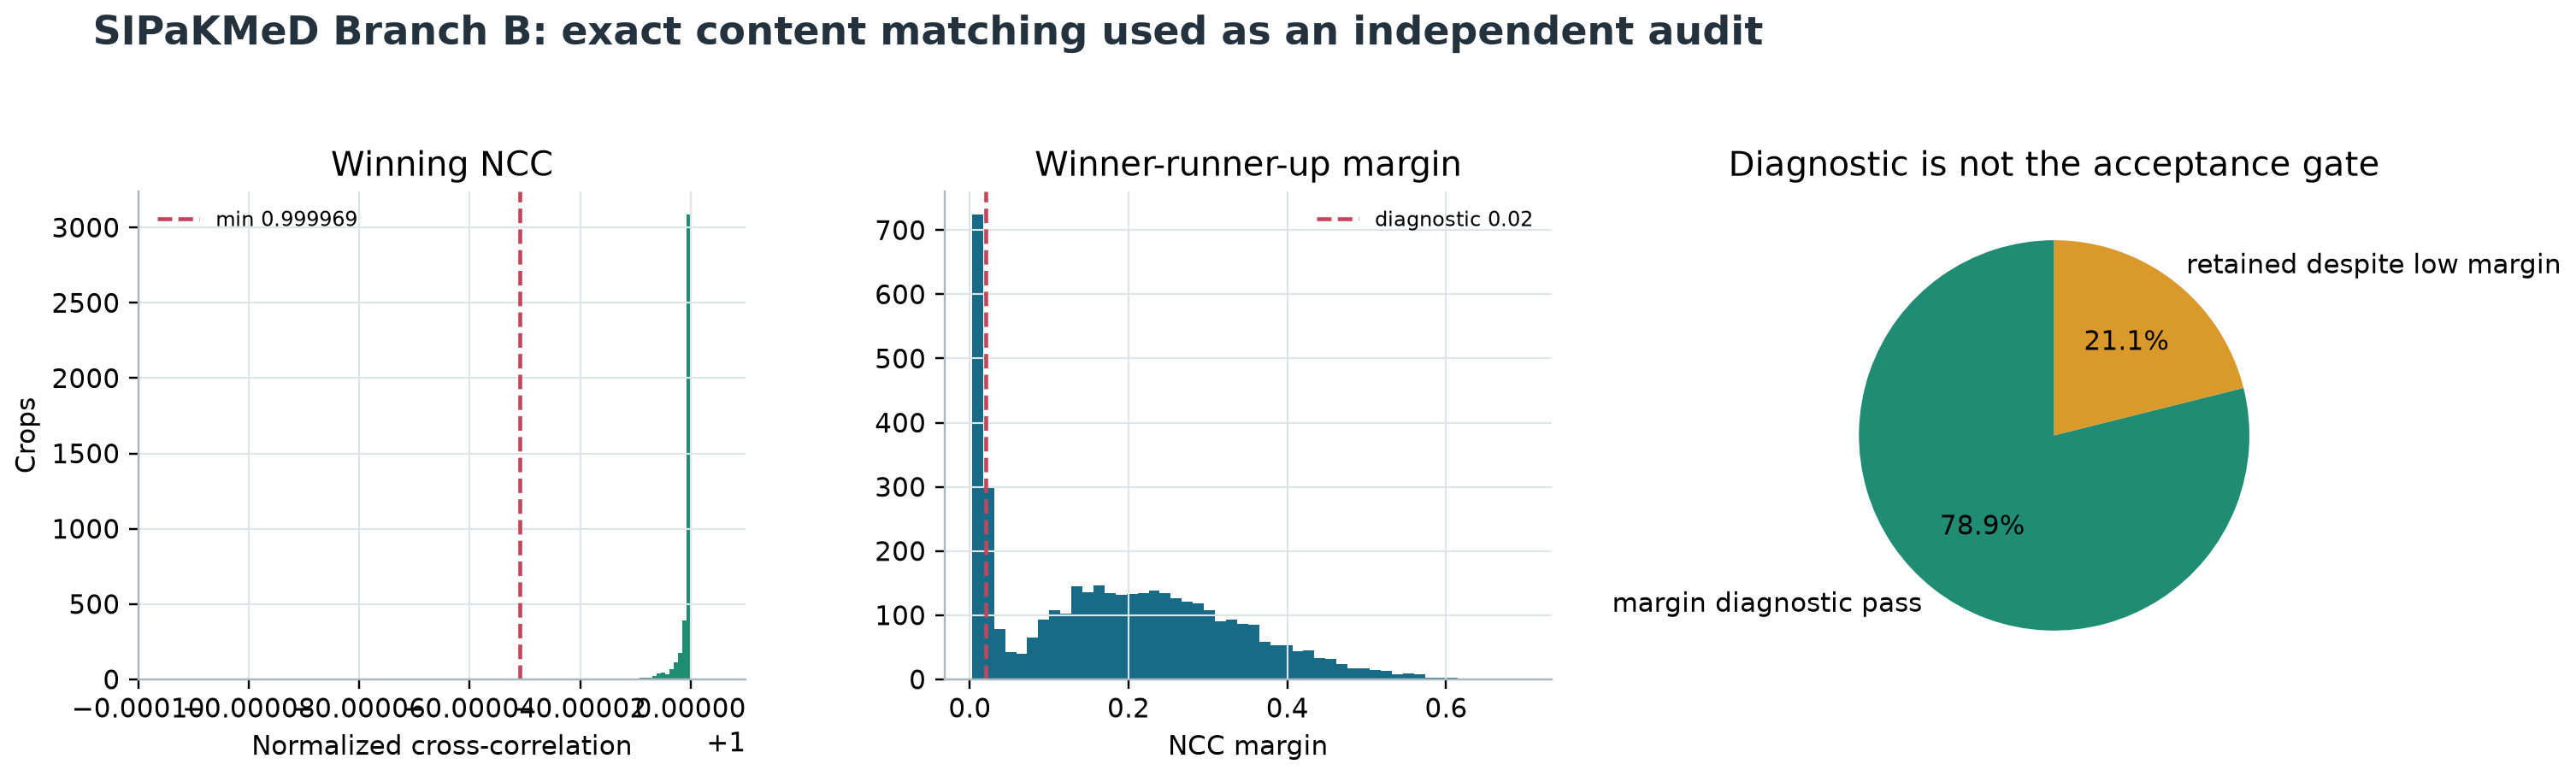
\includegraphics[width=\textwidth]{provenance_diagnostics.png}
\caption{Branch-B diagnostics. The minimum winning NCC is 0.999969. The 0.02 runner-up-margin rule is intentionally only a diagnostic: 3,195 crops pass it and 854 do not, yet all rows agree with Branch A and all boxes remain contained.}
\label{s1:fig:provenance-diagnostics}
\end{figure}

\begin{figure}[H]
\centering
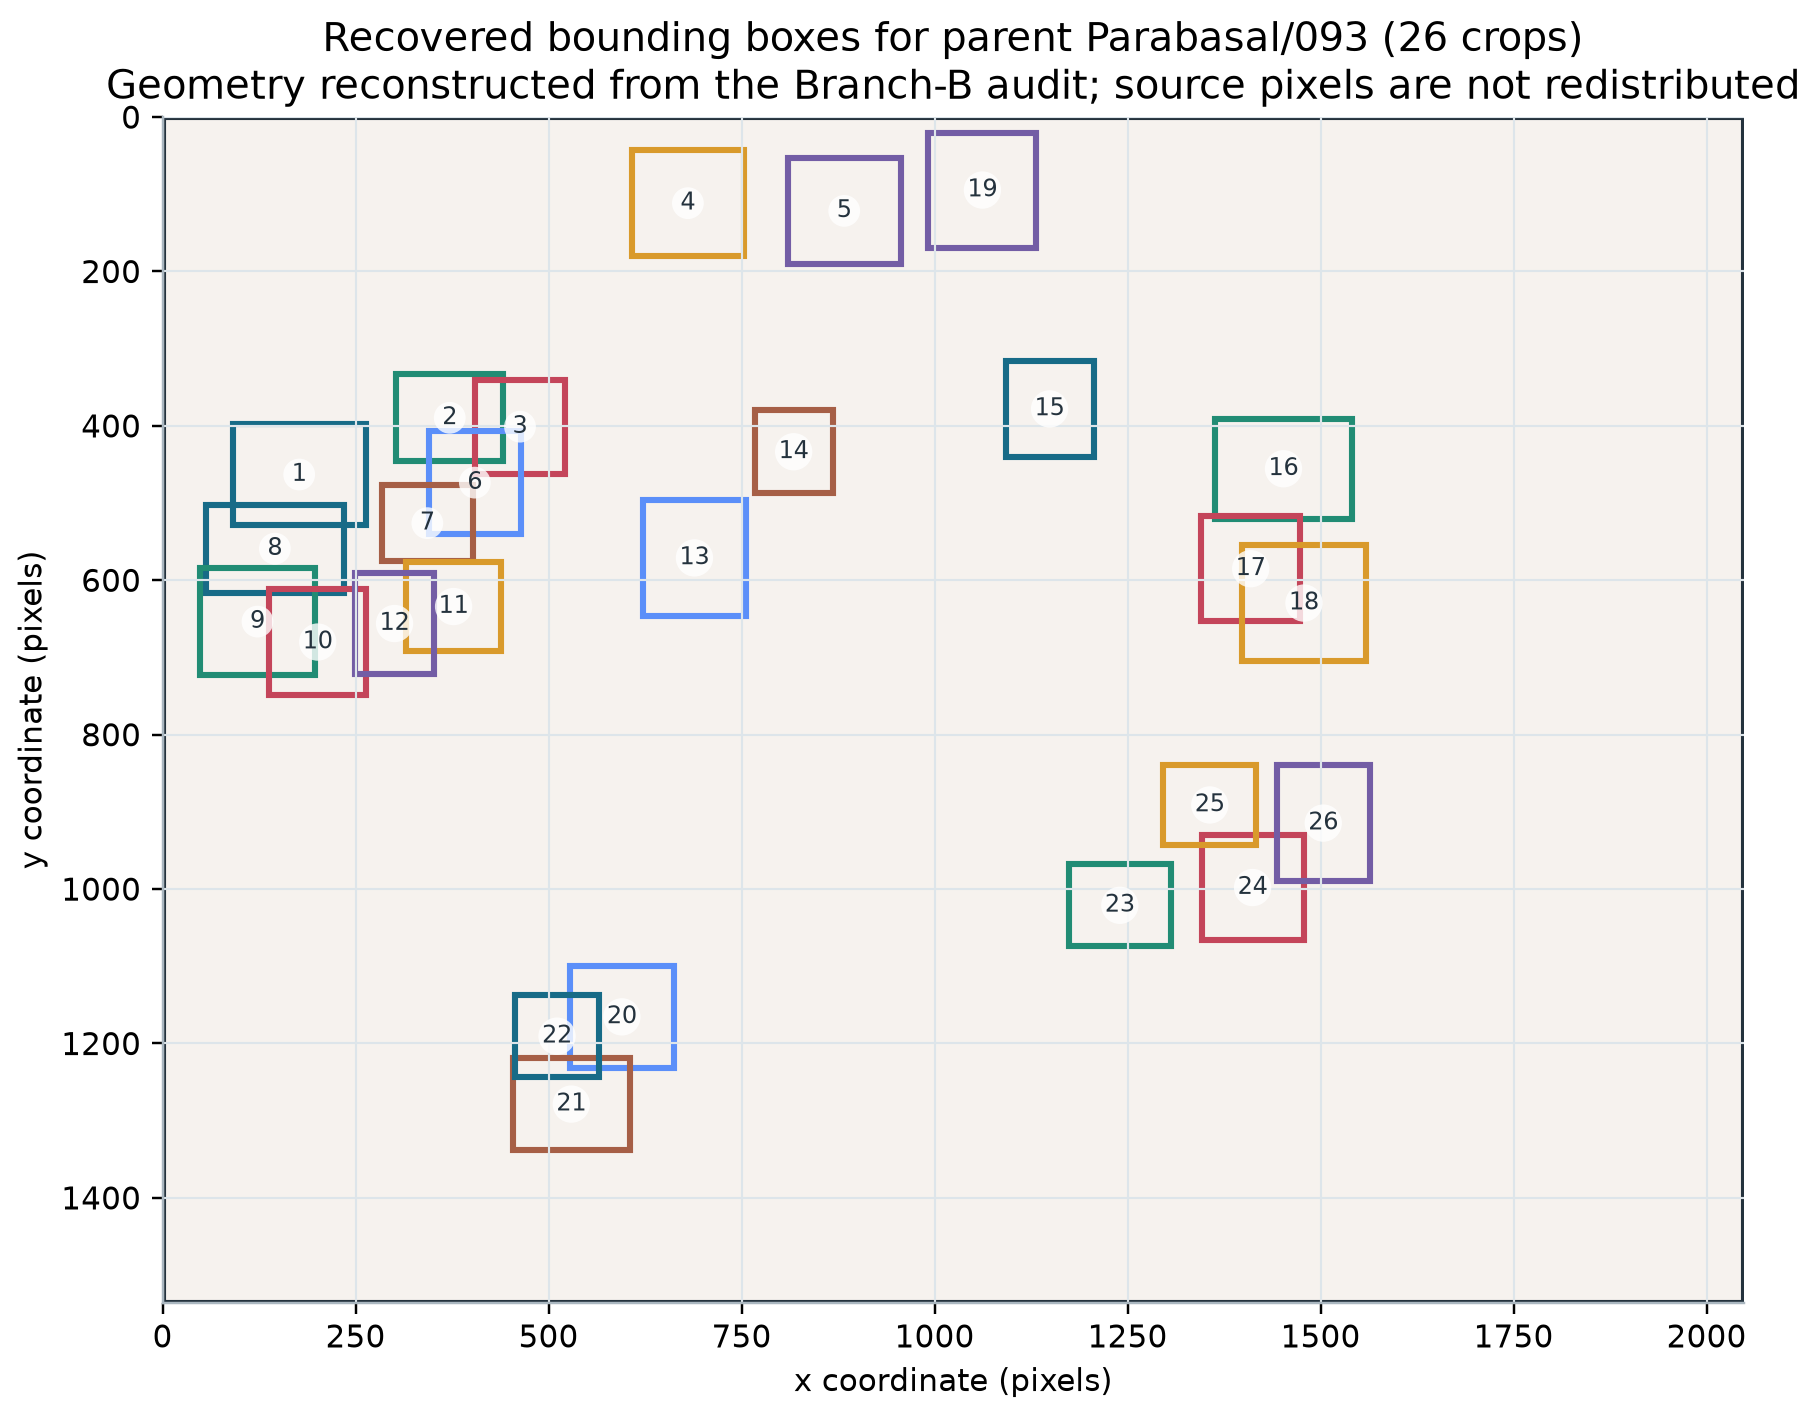
\includegraphics[width=0.77\textwidth]{recovered_bbox_example.png}
\caption{A real recovered-coordinate example for the parent with the largest crop count. Only rectangle geometry is displayed; source pixels are not redistributed. Overlapping rectangles make literal source-pixel sharing possible.}
\label{s1:fig:bboxes}
\end{figure}

\section{Why the auxiliary acceptance flag is false for many correct rows}

The \artifact{accepted} field in Branch B encodes a conservative confidence-plus-margin diagnostic. It is not the registered provenance acceptance outcome. Many microscope fields contain visually repetitive background, so a correct near-perfect winner can have another near-perfect candidate. Substituting this diagnostic for the registered 99\% cross-branch agreement rule would discard 854 correctly mapped crops after looking at an arbitrary margin. The project instead retains every row and exposes the ambiguity measure.

\section{Cx22, CRIC, and Herlev recovery}

Cx22 uses source names and ROI coordinates decoded from the authors' three MATLAB generator releases. Every source resolves against the declared 686-image CCEDD set, and rare edge-touching requested boxes are clipped exactly as the generator code specifies. The released Cx22 archives contain generator metadata and masks rather than a second independent RGB crop array, so an A/B image-content branch cannot be constructed from the public package alone. Applicable checks are source existence, exact metadata decoding, generator geometry, bounds, and subset overlap.

CRIC uses the released classifications table: source-image identity and coordinates directly define the map. Herlev assigns each released cell to itself. Neither route pretends to recover unavailable patient identity.

\section{Verification outcome}

\begin{table}[H]
\centering
\caption{Provenance gates.}
\label{s1:tab:provenance-gates}
\begin{tabularx}{\textwidth}{lrrXl}
\toprule
Dataset & Observations & Parents & Applied evidence & Outcome \\
\midrule
SIPaKMeD & 4,049 & 966 & 4,049/4,049 A/B agreement; 4,049 contained boxes; exact class totals & \pass \\
Cx22 & 1,320 & 514 & generator names/ROIs; 686 sources resolve; 1,320 contained clipped boxes & \pass \\
CRIC & 11,534 & 400 & released source identities and coordinates; no patient-ID claim & \pass \\
Herlev & 917 & 917 & one released cell per parent & \pass \\
\bottomrule
\end{tabularx}
\end{table}

No observation was excluded. The five SIPaKMeD parent counts are exactly 126/108/238/271/223 in corrected release order. All crop counts sum to 4,049.

% Carried over verbatim from monograph/main.tex (Study 1 record, 13 Sep 2026).
\chapter{Split protocols and structural leakage}\label{s1:ch:ch07_split_protocols_and_structural_leakage}

\section{Why four protocols are needed}

\begin{figure}[H]
\centering
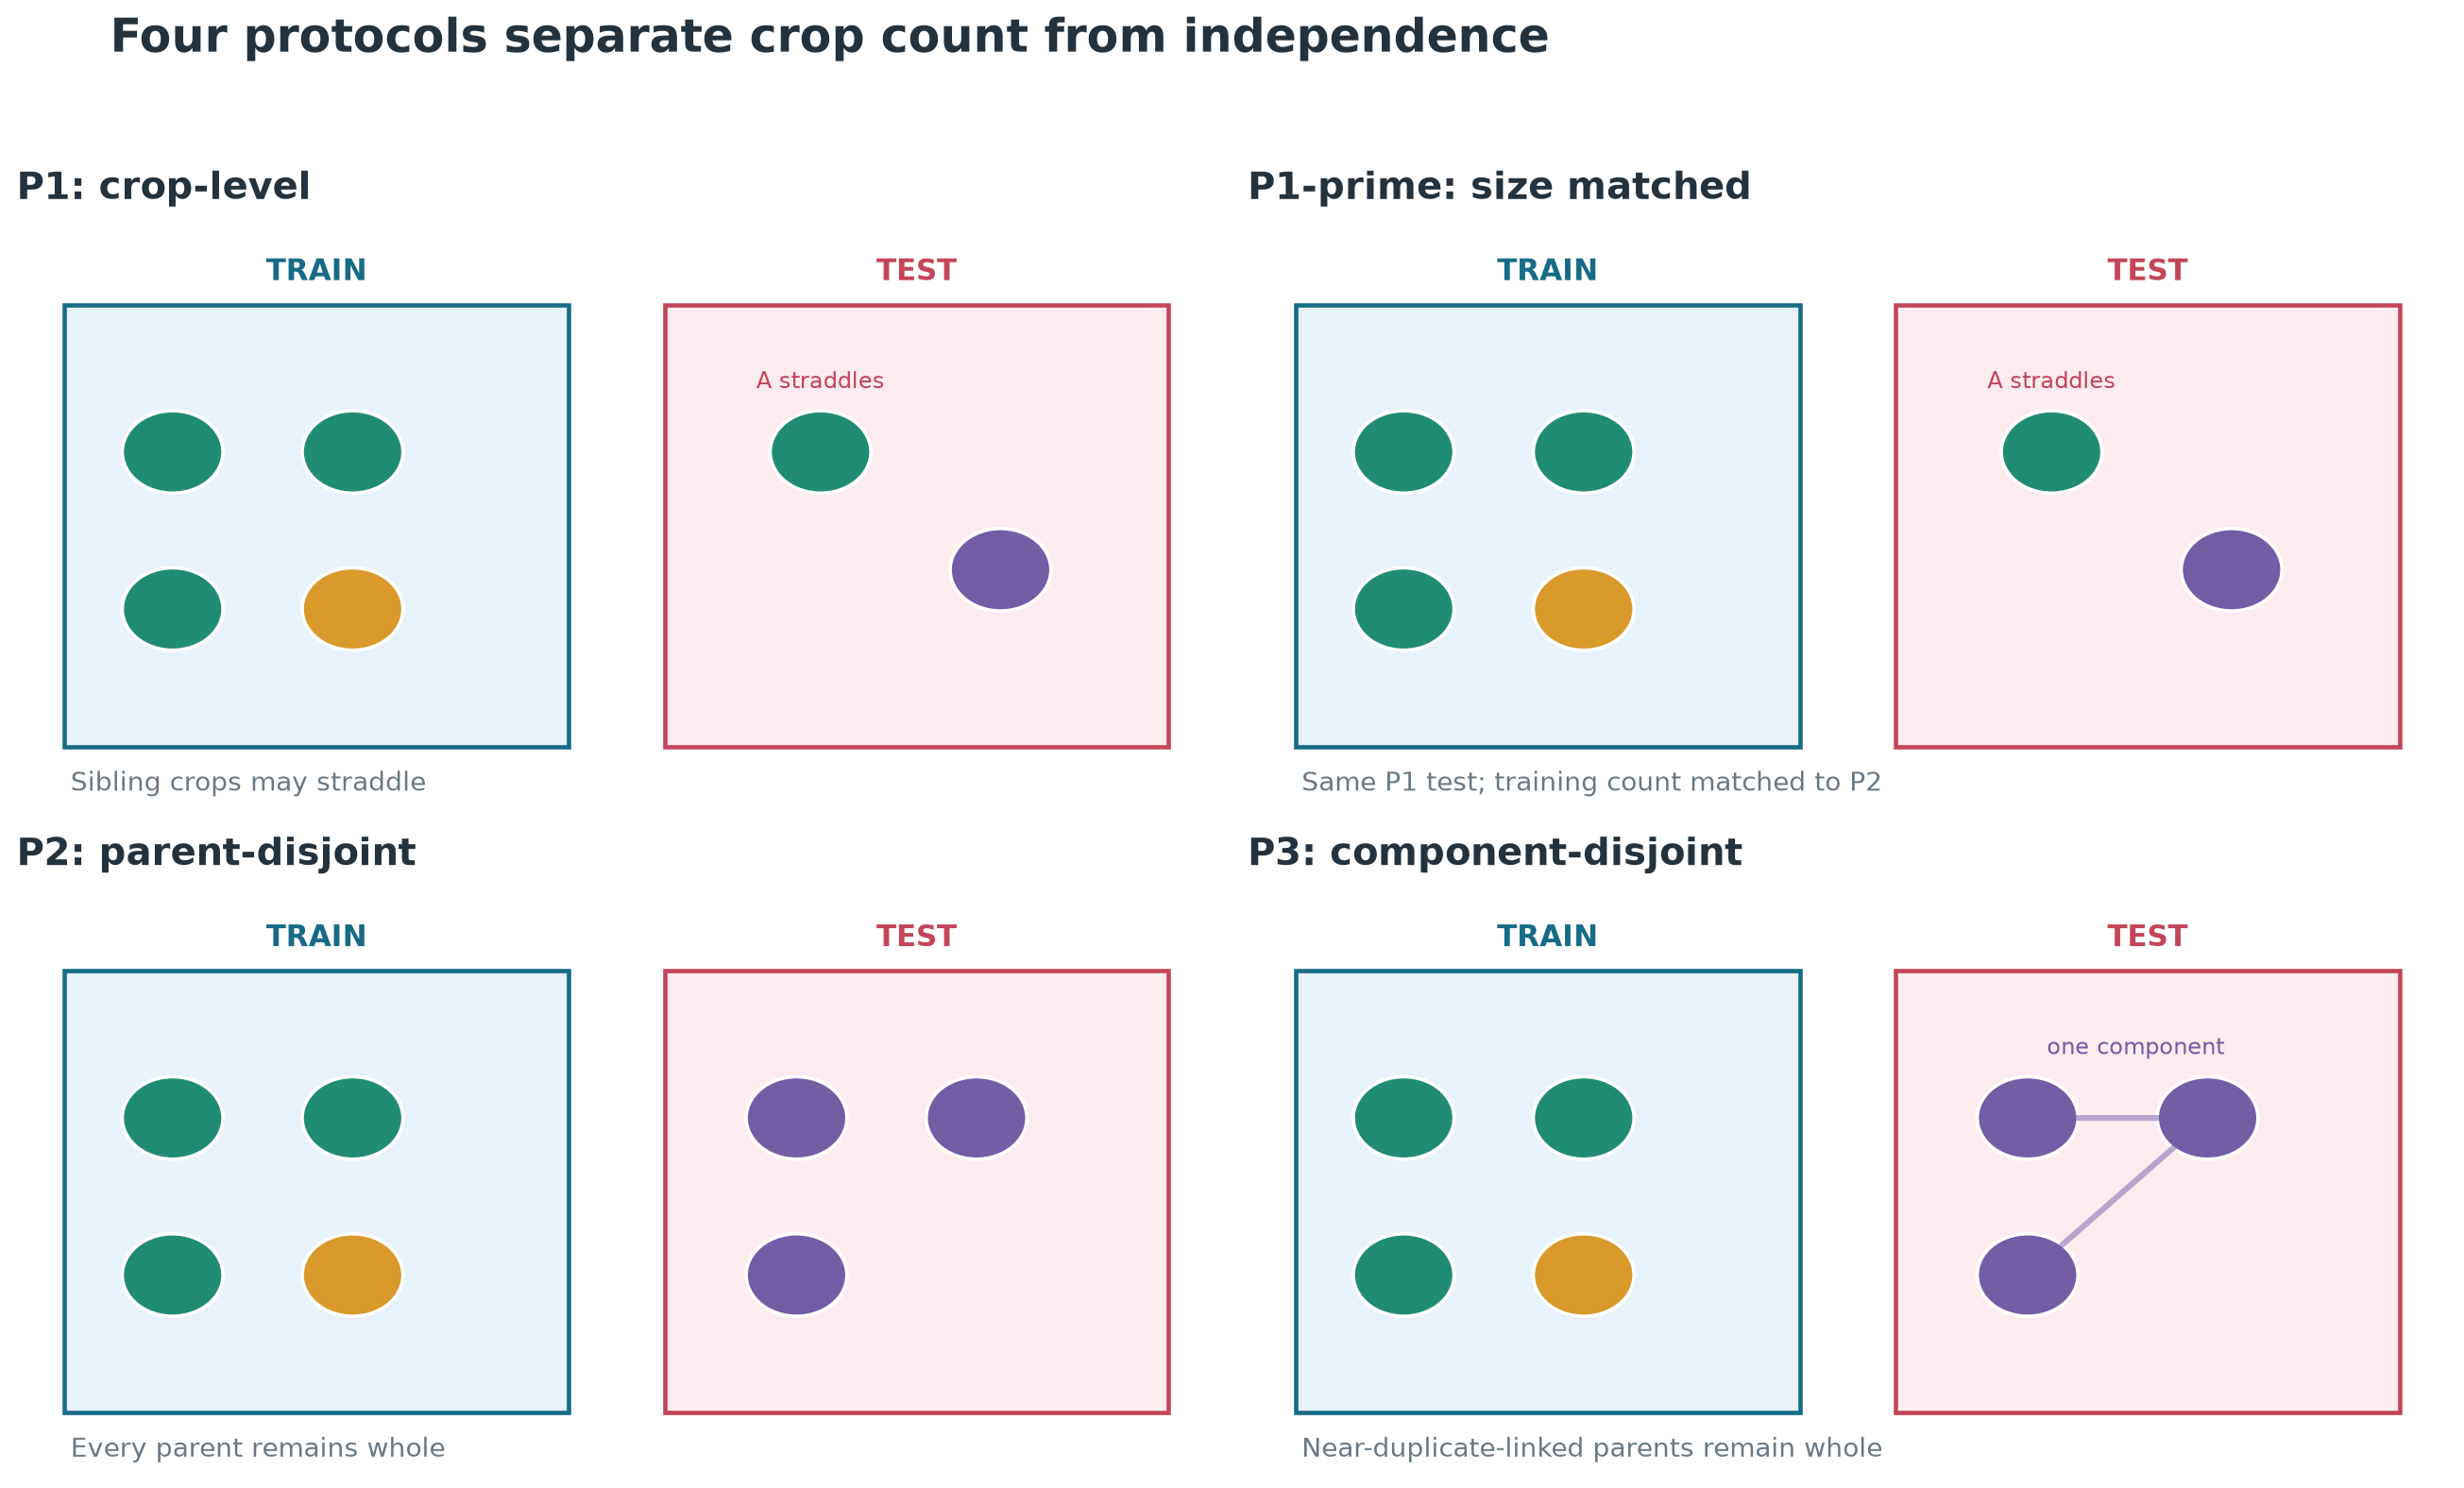
\includegraphics[width=\textwidth]{split_protocols.png}
\caption{The four protocols. P1 asks what common crop splitting shares. P1-prime holds its test set but matches the P2 training count. P2 groups exact parents. P3 groups whole near-duplicate-linked parent components.}
\label{s1:fig:protocols}
\end{figure}

All splits use an 80:20 target and the five fixed seeds. P1 is class-stratified at crop level. P1-prime retains P1's test observations and downsamples only its training observations to exactly the P2 training count, as closely class-balanced as integer counts permit. P2 uses group-aware allocation by exact parent. P3 repeats parent-disjoint allocation after cross-parent candidate links are collapsed into connected components.

On the frozen SIPaKMeD environment, P2 contains 3,239 train and 810 test crops for every seed. P1 already has exactly those counts, so P1-prime is identical to P1. This is not a redundant hidden comparison: it shows that the primary P1--P2 difference cannot be attributed to a larger P1 training set in this implementation.

\section{Analytic straddle probability}

For a parent with $k$ crops independently assigned to training with probability 0.8 and test with probability 0.2, the only non-straddling outcomes are ``all train'' and ``all test.'' Hence
\begin{align}
P(\text{no straddle}\mid k) &= 0.8^k+0.2^k,\\
P(\text{straddle}\mid k) &= 1-0.8^k-0.2^k.
\end{align}
For a dataset with parent crop counts $k_1,\dots,k_m$, the analytic expectation is
\begin{equation}
\bar{P}_{\text{straddle}}=\frac{1}{m}\sum_{j=1}^{m}\left(1-0.8^{k_j}-0.2^{k_j}\right).
\end{equation}

The exact class-stratified fixed-size splitter is not perfectly independent Bernoulli assignment. Therefore the analytic quantity is checked against a 10,000-allocation Monte Carlo interval generated with the actual count vector and allocation rule.

\begin{figure}[H]
\centering
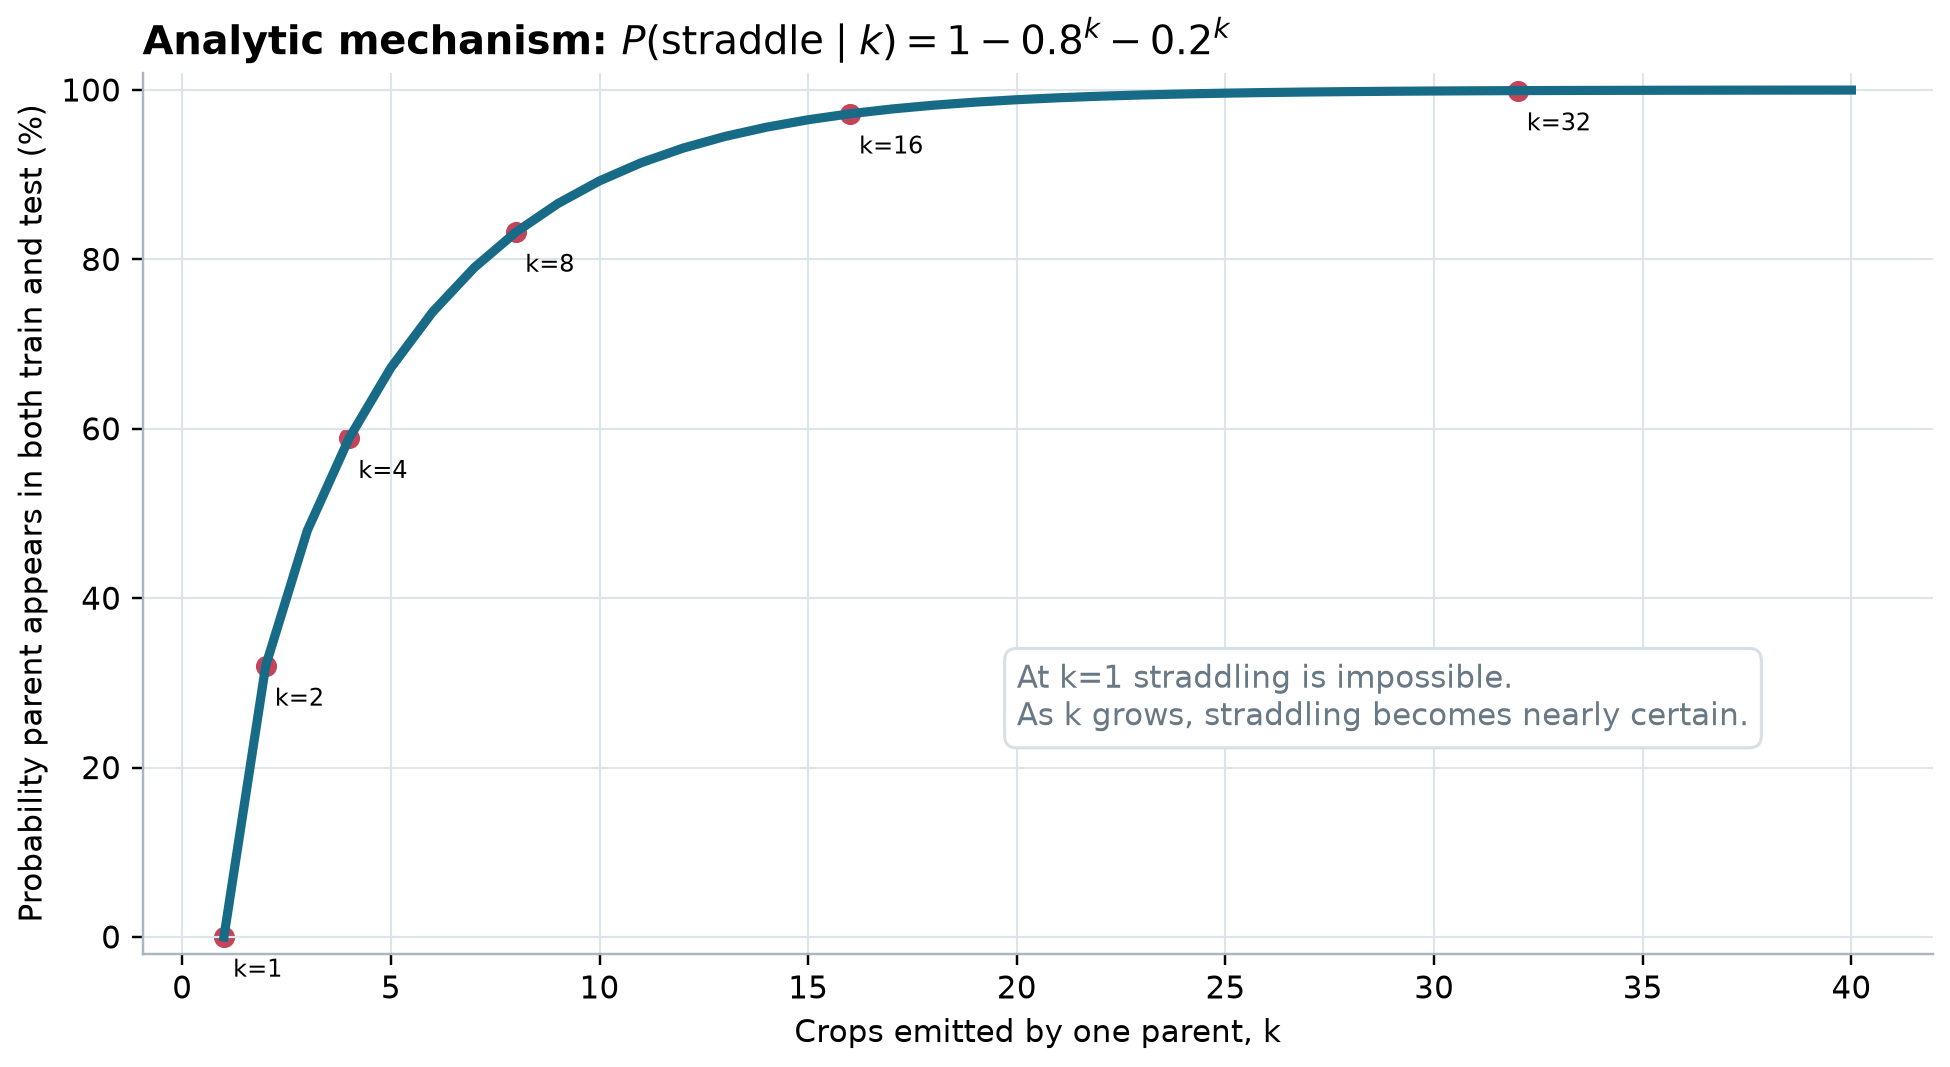
\includegraphics[width=0.87\textwidth]{straddle_probability.png}
\caption{The analytic mechanism. A one-crop parent cannot straddle; a high-multiplicity parent almost certainly straddles under independent 80:20 crop allocation.}
\label{s1:fig:straddle-curve}
\end{figure}

\section{Structural endpoints}

Let $G_{\mathrm{tr}}$ and $G_{\mathrm{te}}$ be training and test parent sets, and let $T$ be the test observations. The parent-straddle fraction and leaked-test-observation fraction are
\begin{equation}
L_p=\frac{|G_{\mathrm{tr}}\cap G_{\mathrm{te}}|}{|G|},\qquad
L_c=\frac{1}{|T|}\sum_{x\in T}\mathbf{1}\{g(x)\in G_{\mathrm{tr}}\}.
\end{equation}

\begin{table}[H]
\centering
\caption{Structural leakage. Stochastic values are mean $\pm$ sample SD over five seeds.}
\label{s1:tab:structural}
\resizebox{\textwidth}{!}{%
\begin{tabular}{lrrrrrr}
\toprule
Dataset & Crops & Parents & Analytic P1 straddle & Observed P1 straddle & P1 test with train parent & P2/P3 straddle \\
\midrule
SIPaKMeD & 4,049 & 966 & 44.83\% & 45.63$\pm$1.04\% & 92.62$\pm$0.40\% & 0.00$\pm$0.00\% \\
Cx22 & 1,320 & 514 & 33.93\% & 34.01$\pm$1.10\% & 85.23$\pm$3.51\% & 0.00$\pm$0.00\% \\
CRIC & 11,534 & 400 & 94.88\% & 94.35$\pm$1.10\% & 99.97$\pm$0.08\% & 0.00$\pm$0.00\% \\
Herlev & 917 & 917 & 0.00\% & 0.00$\pm$0.00\% & 0.00$\pm$0.00\% & 0.00$\pm$0.00\% \\
\bottomrule
\end{tabular}}
\end{table}

\begin{figure}[H]
\centering
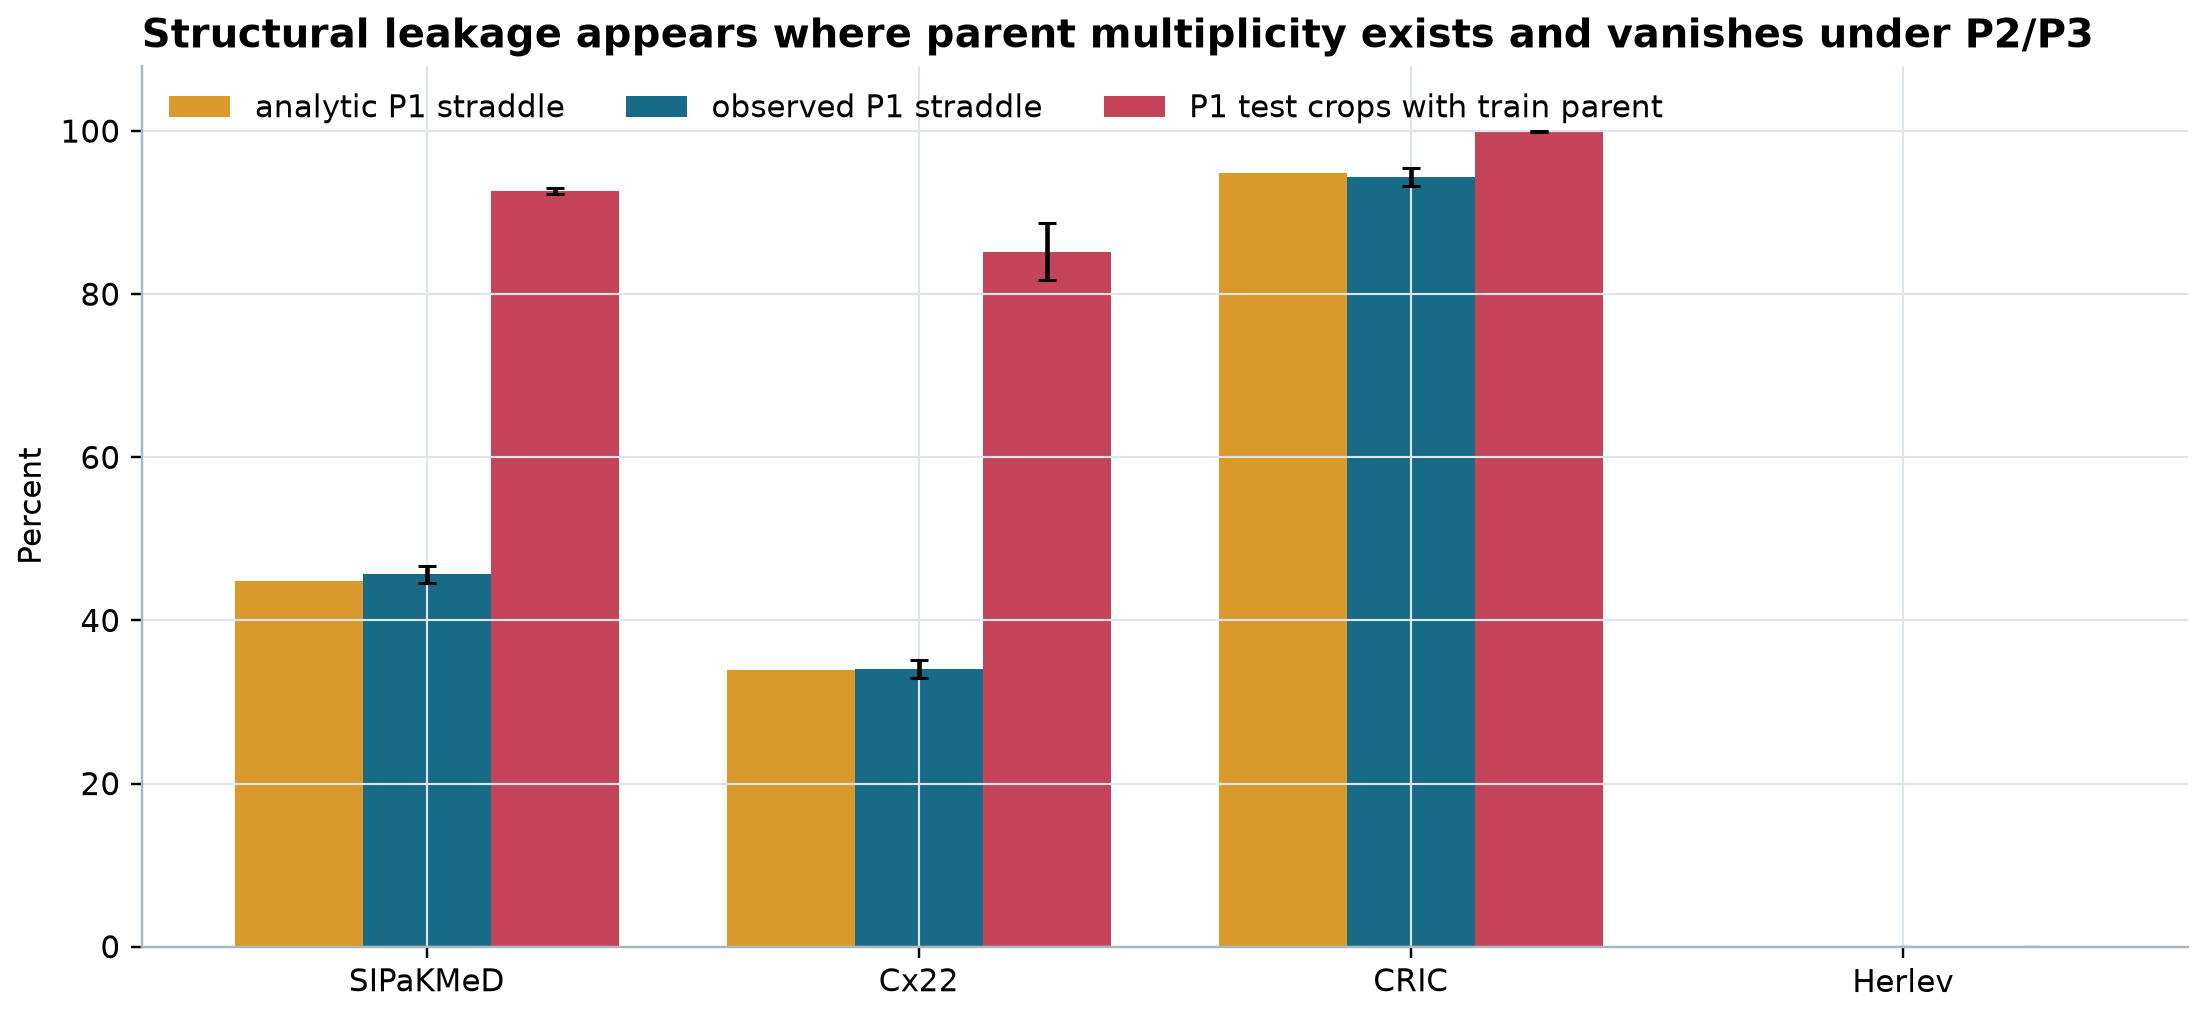
\includegraphics[width=\textwidth]{structural_results.png}
\caption{Analytic and observed leakage. P2 and P3 are omitted from the bars because both are exactly zero on all four datasets.}
\label{s1:fig:structural-results}
\end{figure}

\begin{figure}[H]
\centering
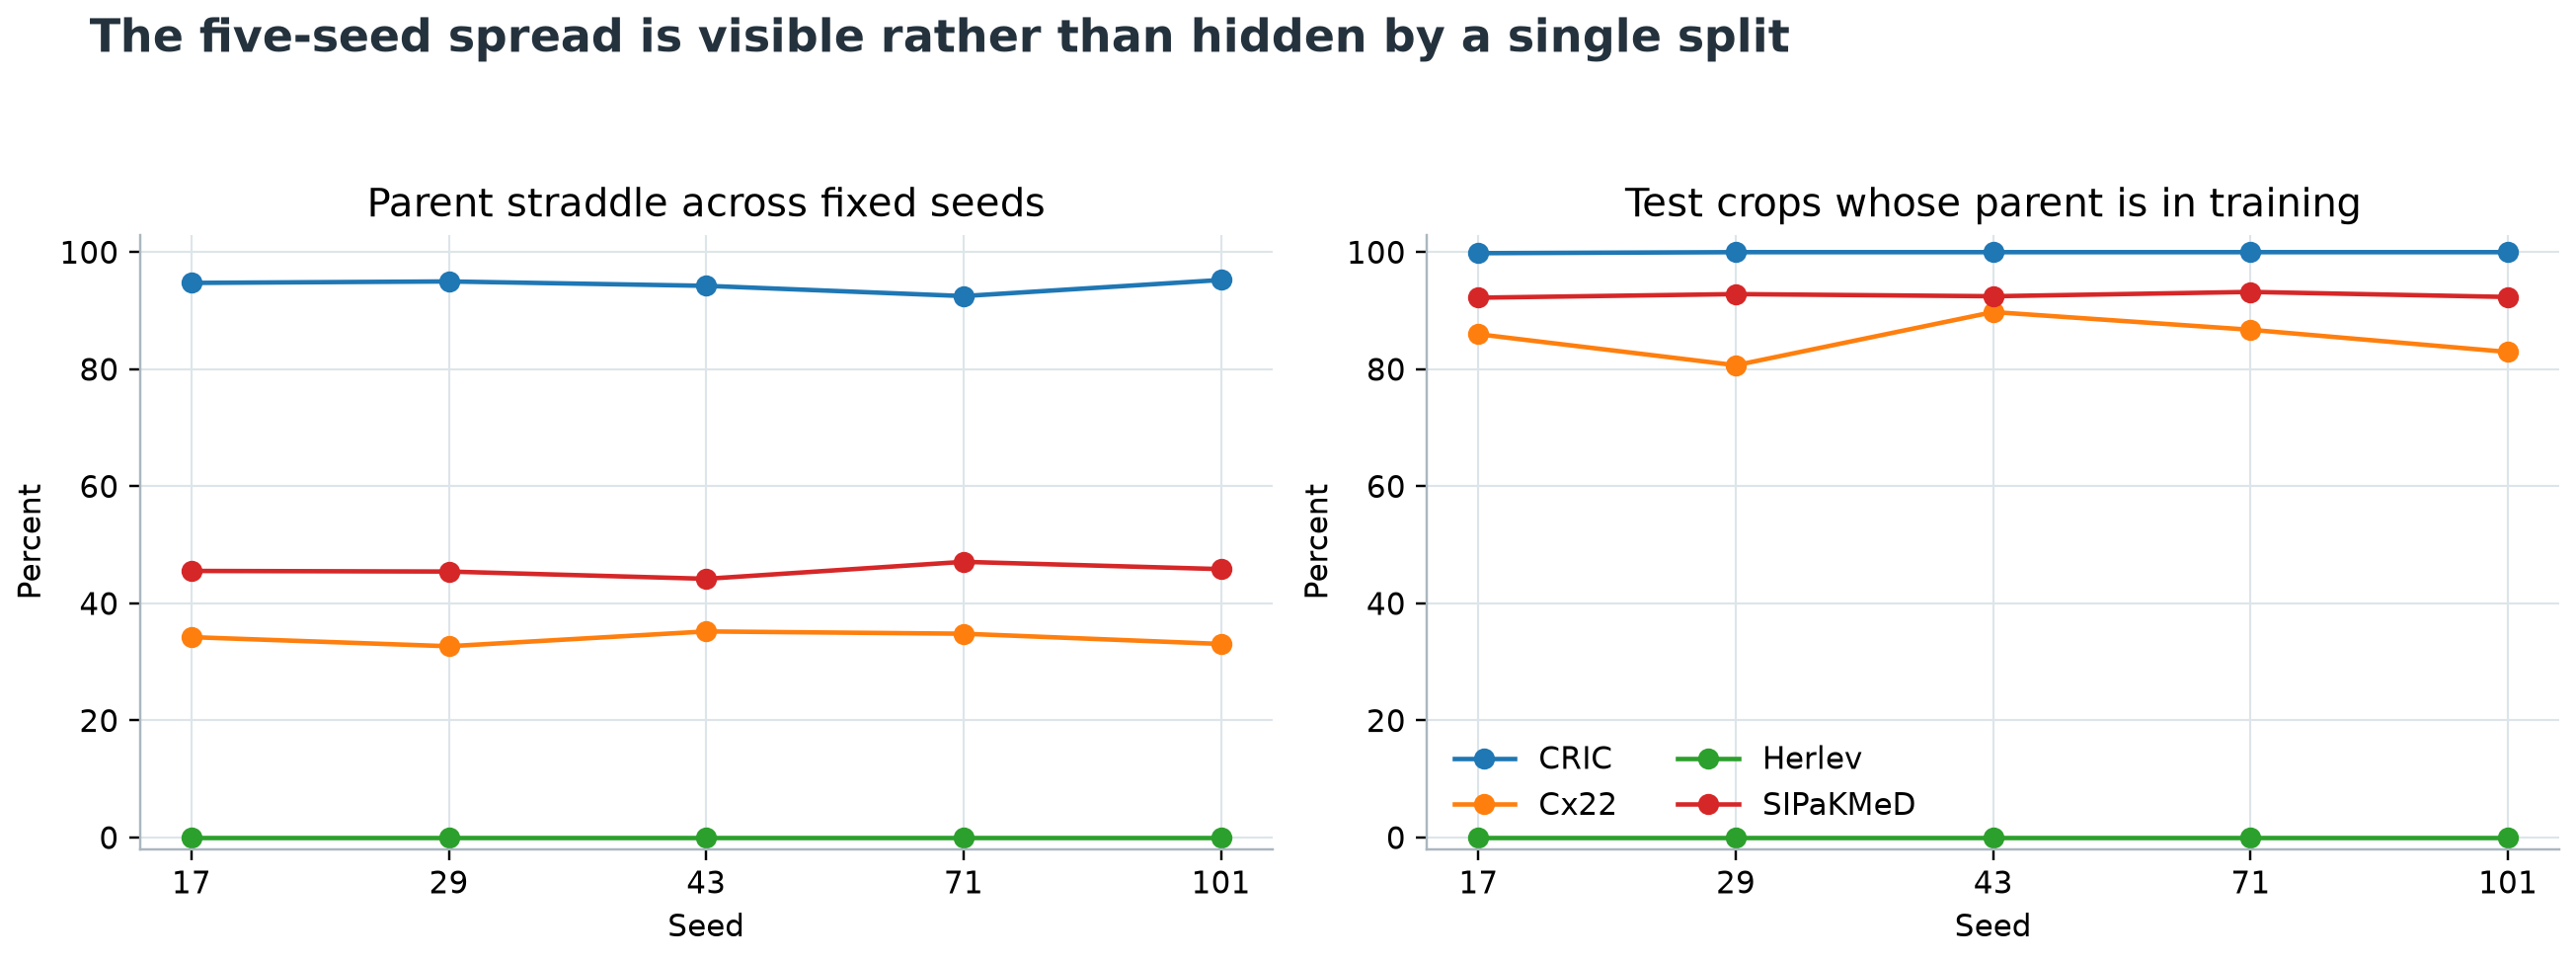
\includegraphics[width=\textwidth]{structural_seed_spread.png}
\caption{Seed-level structural results. Reporting the spread prevents one convenient split from defining the claim.}
\label{s1:fig:structural-seeds}
\end{figure}

\section{Interpretation}

CRIC is the most extreme because its parents emit 28.84 crops on average: essentially every random-split test cell has a source image in training. SIPaKMeD and Cx22 have lower parent multiplicity, yet 92.62\% and 85.23\% of their test observations respectively still have a training sibling. Herlev establishes implementation specificity: the same code returns zero when the data genuinely have one observation per parent.

The structural ordering P3 $\leq$ P2 $\leq$ P1 passes for all datasets. This statement concerns shared parents, not model scores. Later, the analogous model-score ordering fails for four of six SIPaKMeD classifiers; the two outcomes are logically compatible.

% Carried over verbatim from monograph/main.tex (Study 1 record, 13 Sep 2026).
\chapter{Literal overlap and conservative duplicate grouping}\label{s1:ch:ch08_literal_overlap_and_conservative_duplica}

\section{Literal source-pixel overlap}

SIPaKMeD's recovered boxes permit a stronger question than shared parent identity. Let boxes $B_i$ and $B_j$ come from the same field. Their intersection is non-empty when
\begin{equation}
\max(x_i,x_j)<\min(x_i+w_i,x_j+w_j)
\quad\text{and}\quad
\max(y_i,y_j)<\min(y_i+h_i,y_j+h_j).
\end{equation}
The intersection-over-union is
\begin{equation}
\operatorname{IoU}(B_i,B_j)=\frac{|B_i\cap B_j|}{|B_i\cup B_j|}.
\end{equation}

Across 13,064 within-parent crop pairs, 2,185 share at least one pixel and the maximum IoU is 0.546. Under P1, 16.80$\pm$0.77\% of cross-split sibling pairs overlap and 52.62$\pm$1.97\% of test crops overlap at least one source pixel with a training crop. Both quantities are 0.00$\pm$0.00\% under P2 and P3.

\begin{figure}[H]
\centering
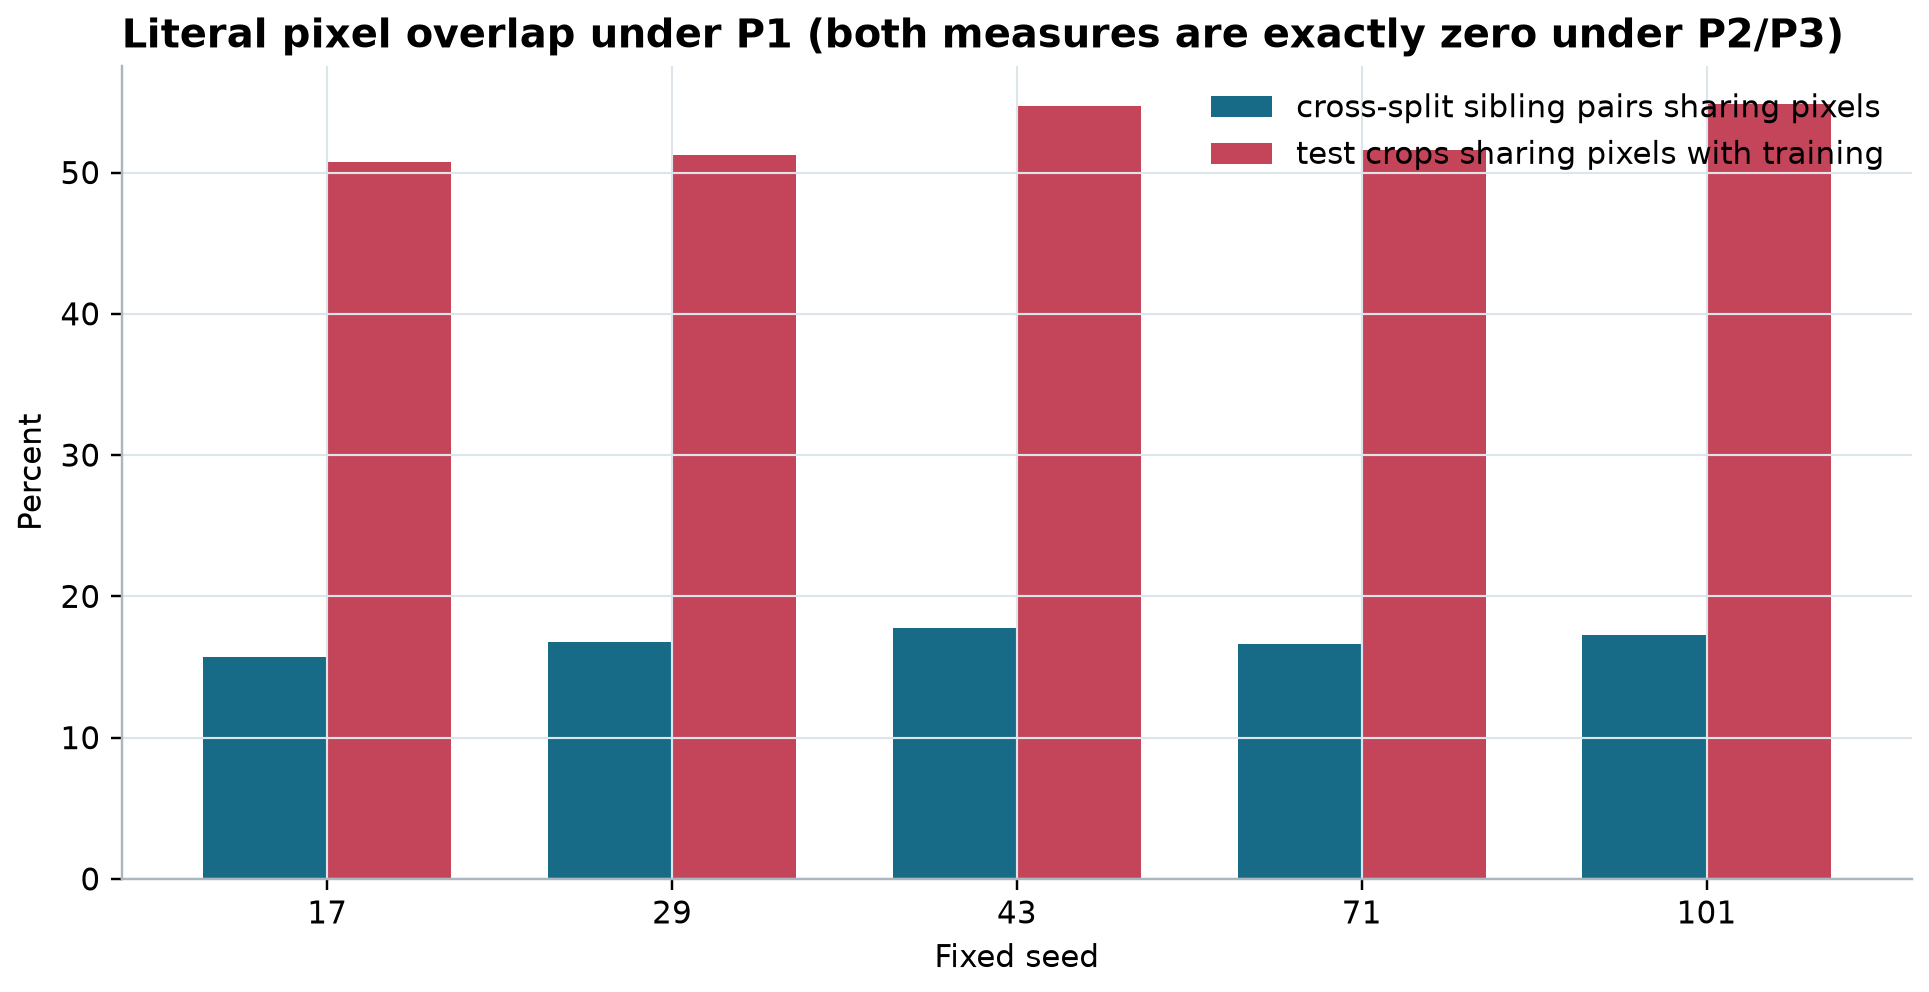
\includegraphics[width=0.9\textwidth]{literal_pixel_overlap.png}
\caption{Literal overlap for every P1 seed. The larger test-crop fraction answers a different question from the pair fraction: whether each test crop has at least one overlapping training sibling.}
\label{s1:fig:pixel-overlap}
\end{figure}

\section{Perceptual hashes and P3}

For each crop the implementation computes a 64-bit perceptual hash from the median-thresholded low-frequency $8\times8$ DCT block and a 64-bit difference hash from adjacent comparisons in an $8\times9$ downsample. Two crops become a candidate pair when they are pixel-exact or when both Hamming distances are at most six. Cross-parent candidate pairs are joined by union-find; each connected component becomes one P3 group.

At the frozen thresholds, the audit found 201 cross-parent candidate pairs. They connect 170 parent IDs into 74 components, the largest containing eight parents, and reduce 966 parents to 870 P3 groups. No pair is pixel-exact. A synthetic calibration detected all three injected transformations and rejected all 100 deterministic unrelated-parent negatives, yielding precision 1.00 and recall 1.00 on that calibration set.

\begin{figure}[H]
\centering
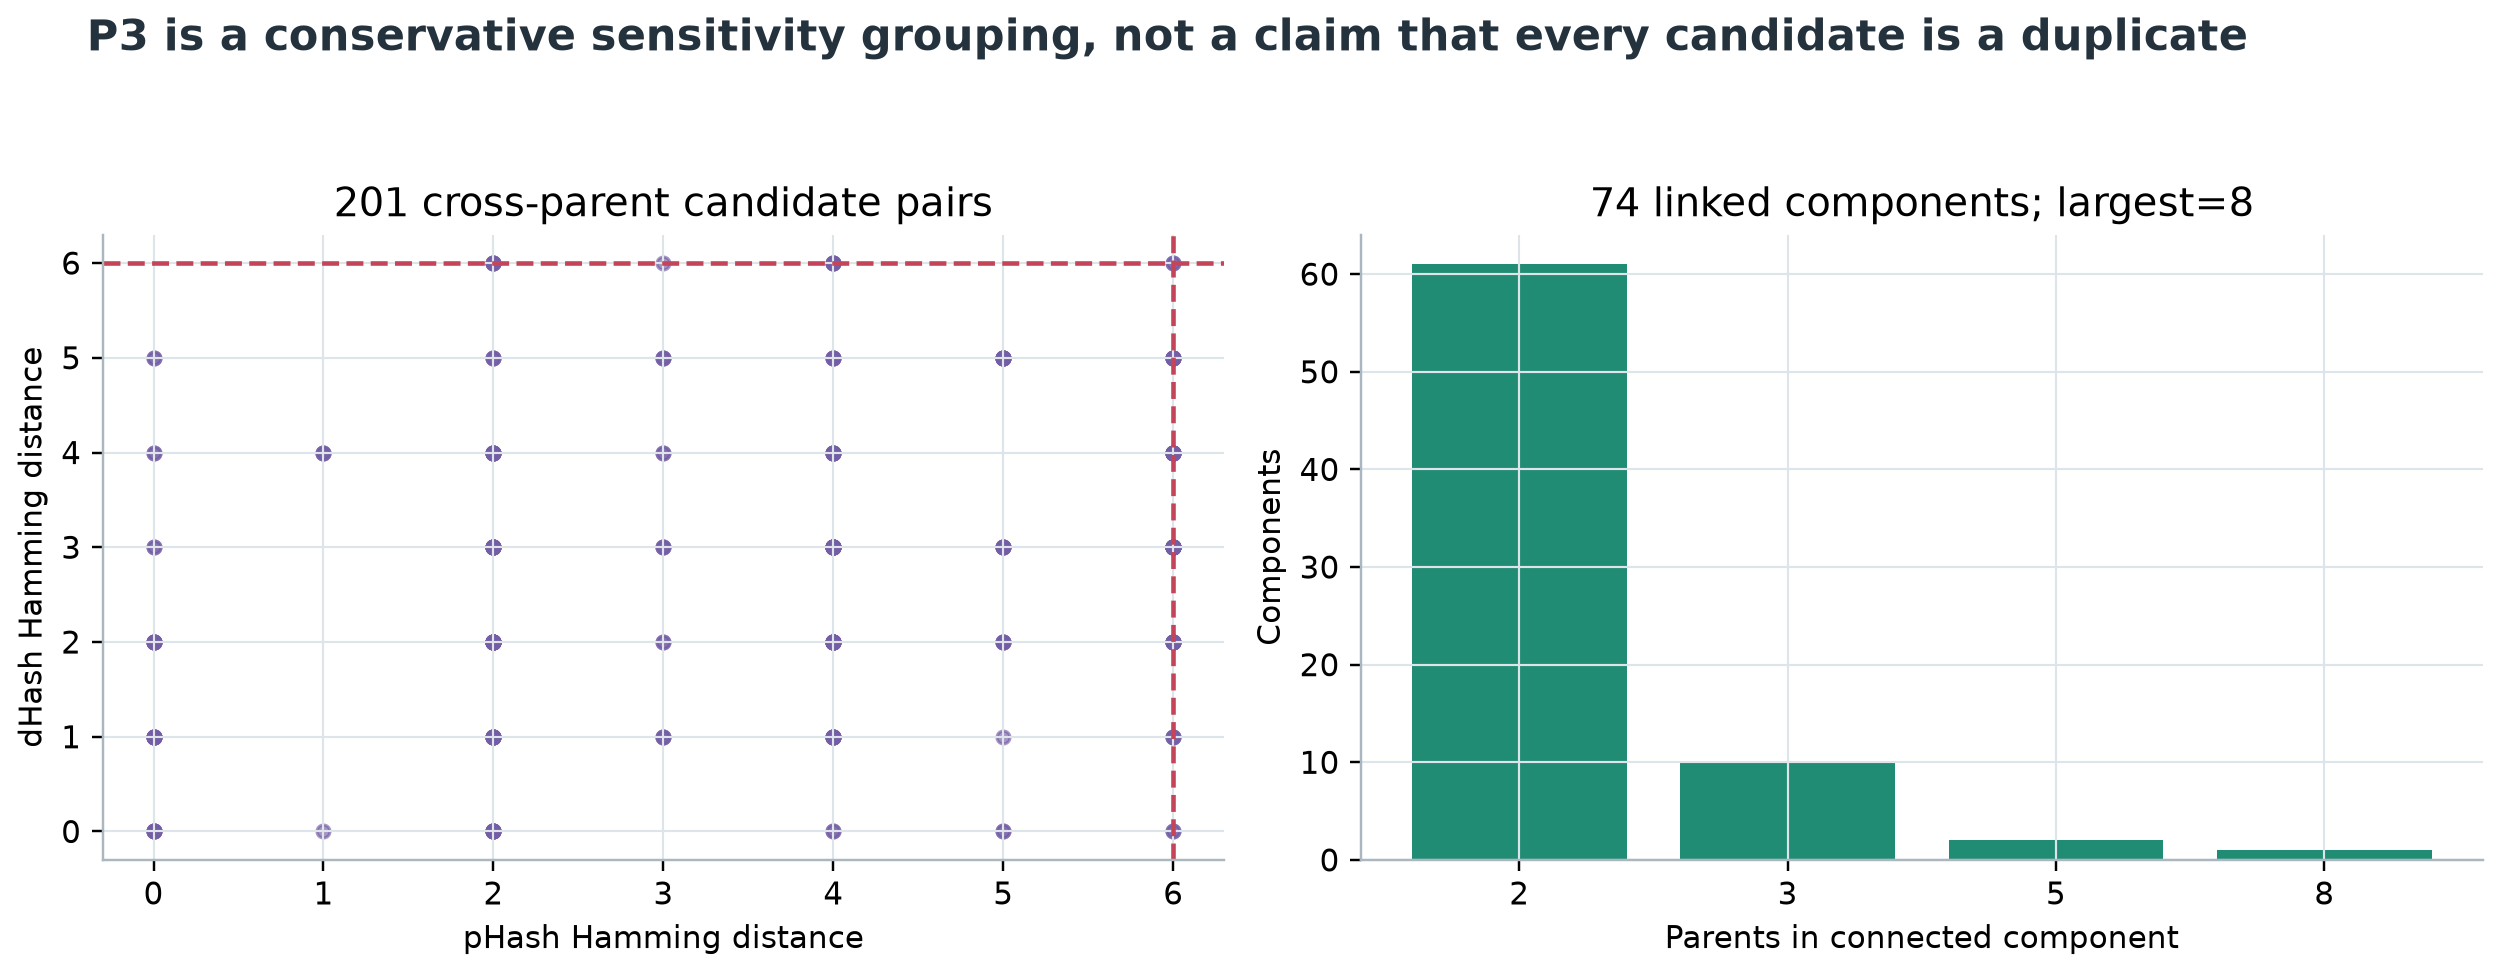
\includegraphics[width=\textwidth]{duplicate_audit.png}
\caption{Near-duplicate sensitivity audit. The thresholded candidates are used conservatively for grouping; they are not treated as ground-truth duplicate annotations.}
\label{s1:fig:duplicates}
\end{figure}

\begin{warningbox}{What the duplicate experiment did not do}
The broader planning idea mentioned a three-detector majority vote involving learned features. The frozen release implements only the pHash+dHash consensus audit and its synthetic calibration. Therefore the report does not claim a CNN/domain-encoder duplicate ensemble, human-confirmed duplicate truth, or general detector precision outside the calibration set.
\end{warningbox}

% Carried over verbatim from monograph/main.tex (Study 1 record, 13 Sep 2026).
\chapter{The parent-identity mechanism probe}\label{s1:ch:ch09_the_parent_identity_mechanism_probe}

\section{Motivation}

Structural overlap says that siblings are present. The parent probe asks whether their shared source is visually recoverable after cellular content and color cues are altered. A positive answer makes the shortcut concrete: a learner can recognize the parent field from a different crop. It still does not prove that a morphology classifier uses that signal.

\section{Balanced task construction}

Parents with at least four crops are eligible. The minimum eligible size allows two training and two test crops per parent. To make chance exact, each eligible parent contributes the same number of training and test crops. The final task contains 424 parents, 848 training crops, and 848 test crops, so chance is
\begin{equation}
P_{\mathrm{chance}}=\frac{1}{424}=0.00235849=0.235849\%.
\end{equation}

A ResNet-18~\cite{he2016resnet} initialized from ImageNet replaces its final layer with a 424-way linear classifier. It trains for 15 epochs with AdamW~\cite{loshchilov2019adamw}, learning rate $10^{-4}$, weight decay $10^{-4}$, batch size 64, and fixed seeds. Training augmentation is a random resized crop with scale 0.85--1.0 plus horizontal and vertical flips; testing resizes to $224\times224$. ImageNet normalization follows every image-mode transform.

\section{Image transformations and their motivations}

\subsection{RGB}
RGB is the maximal-information condition. It permits morphology, stain, illumination, background, focus, acquisition artifacts, and any other visible cue.

\subsection{Grayscale}
Grayscale removes hue and saturation while retaining luminance, edges, morphology, focus, and texture. Persistence here means identity is not solely a stain-color phenomenon.

\subsection{LAB stain normalization}
RGB is converted to CIE LAB. For channel vector $z$, source mean $\mu_s$, source standard deviation $\sigma_s$, and fixed target statistics $\mu_t=(190,140,135)$ and $\sigma_t=(35,14,14)$, the implemented transform is
\begin{equation}
z'=\operatorname{clip}\left((z-\mu_s)\odot\frac{\sigma_t}{\max(\sigma_s,1)}+\mu_t,0,255\right).
\end{equation}
This is a fixed-statistics color-transfer normalization based on the logic of Reinhard et al.~\cite{reinhard2001color}. Persistence means simple first- and second-moment color normalization does not erase the source fingerprint.

\subsection{Background-only: Otsu, morphology, and Telea inpainting}

This condition deliberately removes the likely cell foreground. The implementation converts RGB to HSV and grayscale, then independently obtains Otsu thresholds~\cite{otsu1979threshold} on saturation $S$ and luminance $Y$. The preliminary foreground mask is
\begin{equation}
M_0(u)=\mathbf{1}\{S(u)>t_S\;\lor\;Y(u)<t_Y\}.
\end{equation}
A $5\times5$ morphological closing fills small holes and connects narrow gaps:
\begin{equation}
M=(M_0\oplus K)\ominus K.
\end{equation}
Finally, the marked region is filled from its boundary with Telea's fast-marching inpainting method using radius 5~\cite{telea2004inpainting}. The result keeps background statistics while suppressing the cell body and nucleus. A successful classifier in this condition shows that background alone carries considerable parent information.

\subsection{High-pass}
For Gaussian blur $G_{\sigma=3}*I$, the residual is
\begin{equation}
I_{\mathrm{hp}}=\operatorname{clip}\left(I-G_{\sigma=3}*I+128,0,255\right).
\end{equation}
This suppresses low-frequency illumination and emphasizes local texture, edges, compression, and focus structure.

\begin{figure}[H]
\centering
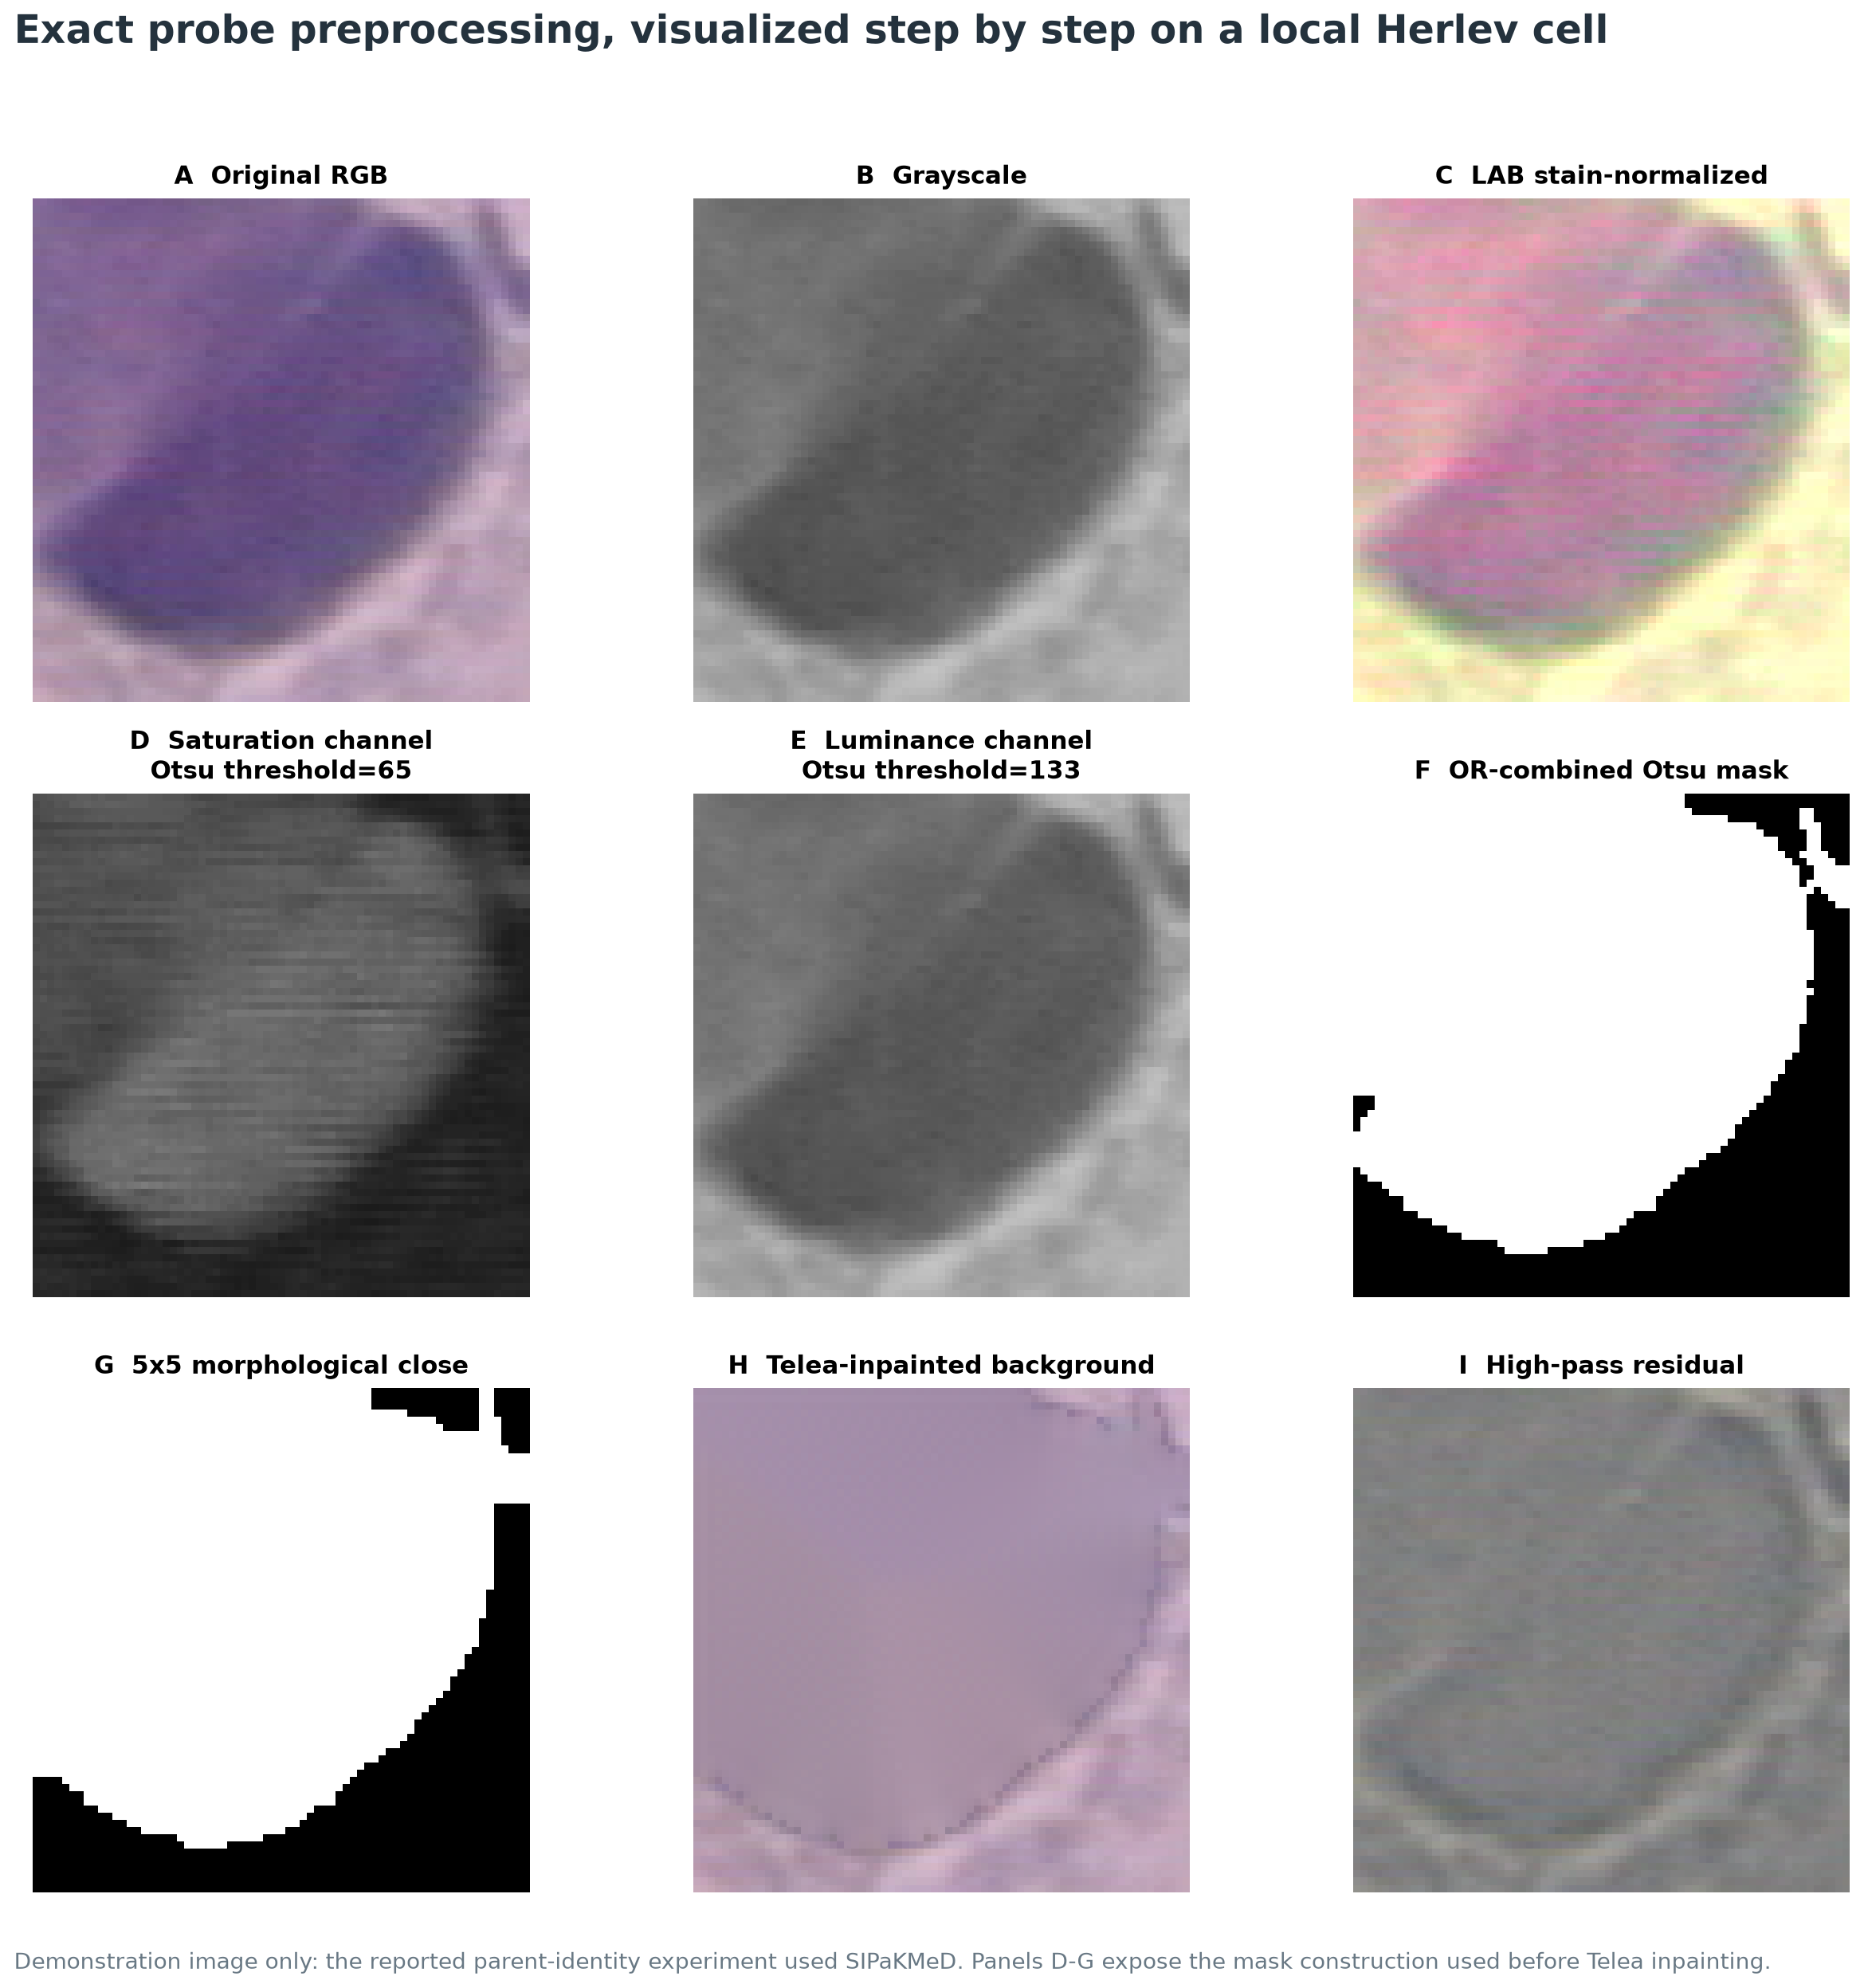
\includegraphics[width=0.92\textwidth]{probe_transformations.png}
\caption{Every preprocessing stage shown on an actual local Herlev cell. This is an implementation demonstration, not a probe result image: the reported parent-identification experiment used SIPaKMeD crops. Panels D--G make Otsu thresholding, mask combination, and morphological closing visible before Telea inpainting.}
\label{s1:fig:transformations}
\end{figure}

\section{Shuffled-label negative control}

Only the training labels are permuted, using the same images, optimizer, epochs, seeds, and task size. The five-seed 95\% interval must cover the exact chance baseline. Otherwise the probe would be rejected because a bookkeeping or imbalance artifact could explain apparent identity learning.

\section{Results}

\begin{table}[H]
\centering
\caption{Parent-identity probe. Mean $\pm$ sample SD over five seeds.}
\label{s1:tab:probe}
\begin{tabular}{lrr}
\toprule
Input condition & Accuracy & Multiple of chance \\
\midrule
RGB & 25.73$\pm$0.66\% & 109.1$\times$ \\
Grayscale & 13.80$\pm$1.12\% & 58.5$\times$ \\
Stain-normalized & 17.31$\pm$0.64\% & 73.4$\times$ \\
Background-only & 18.68$\pm$1.25\% & 79.2$\times$ \\
High-pass & 16.27$\pm$0.60\% & 69.0$\times$ \\
Shuffled RGB labels & 0.17$\pm$0.24\% & 0.7$\times$ \\
\bottomrule
\end{tabular}
\end{table}

\begin{figure}[H]
\centering
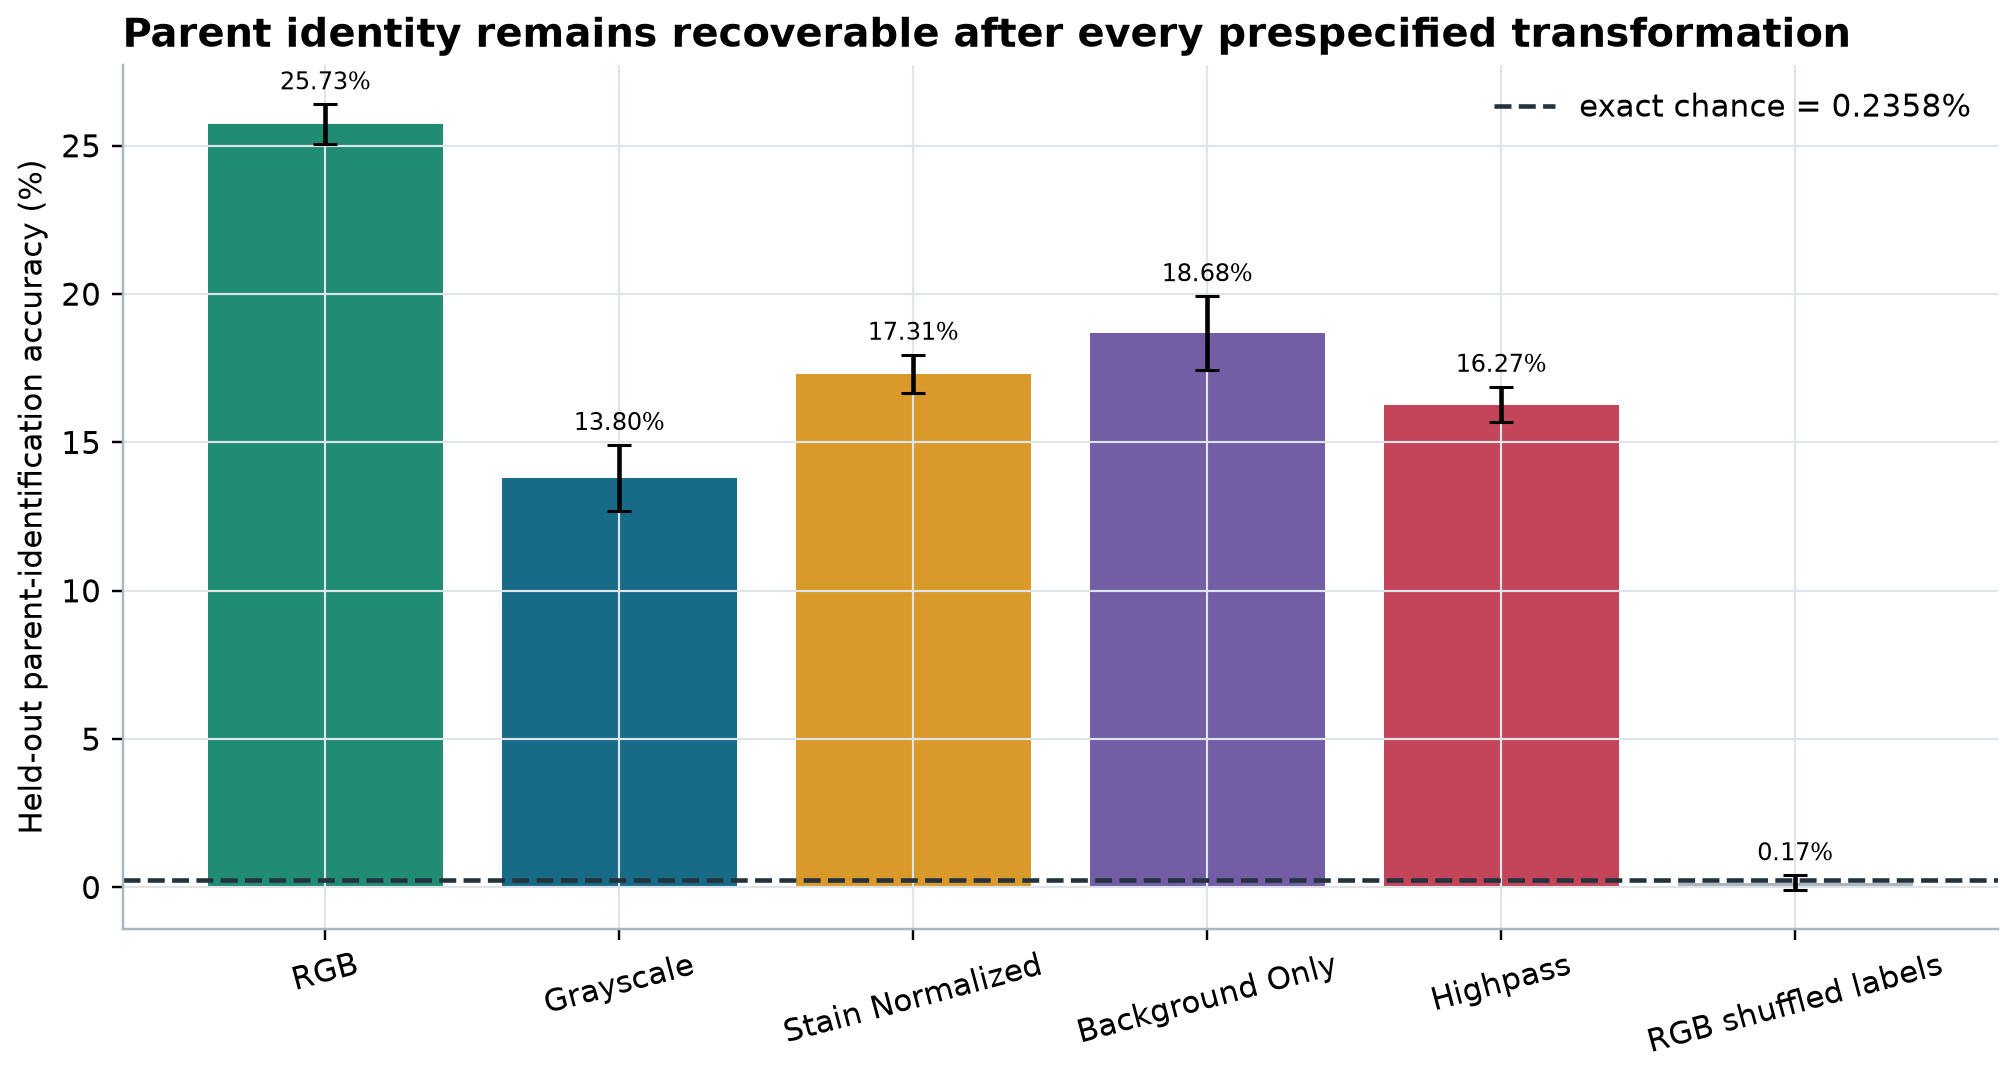
\includegraphics[width=0.92\textwidth]{probe_results.png}
\caption{All prespecified image conditions remain far above chance. Error bars are sample SD across five seeds.}
\label{s1:fig:probe-results}
\end{figure}

\begin{figure}[H]
\centering
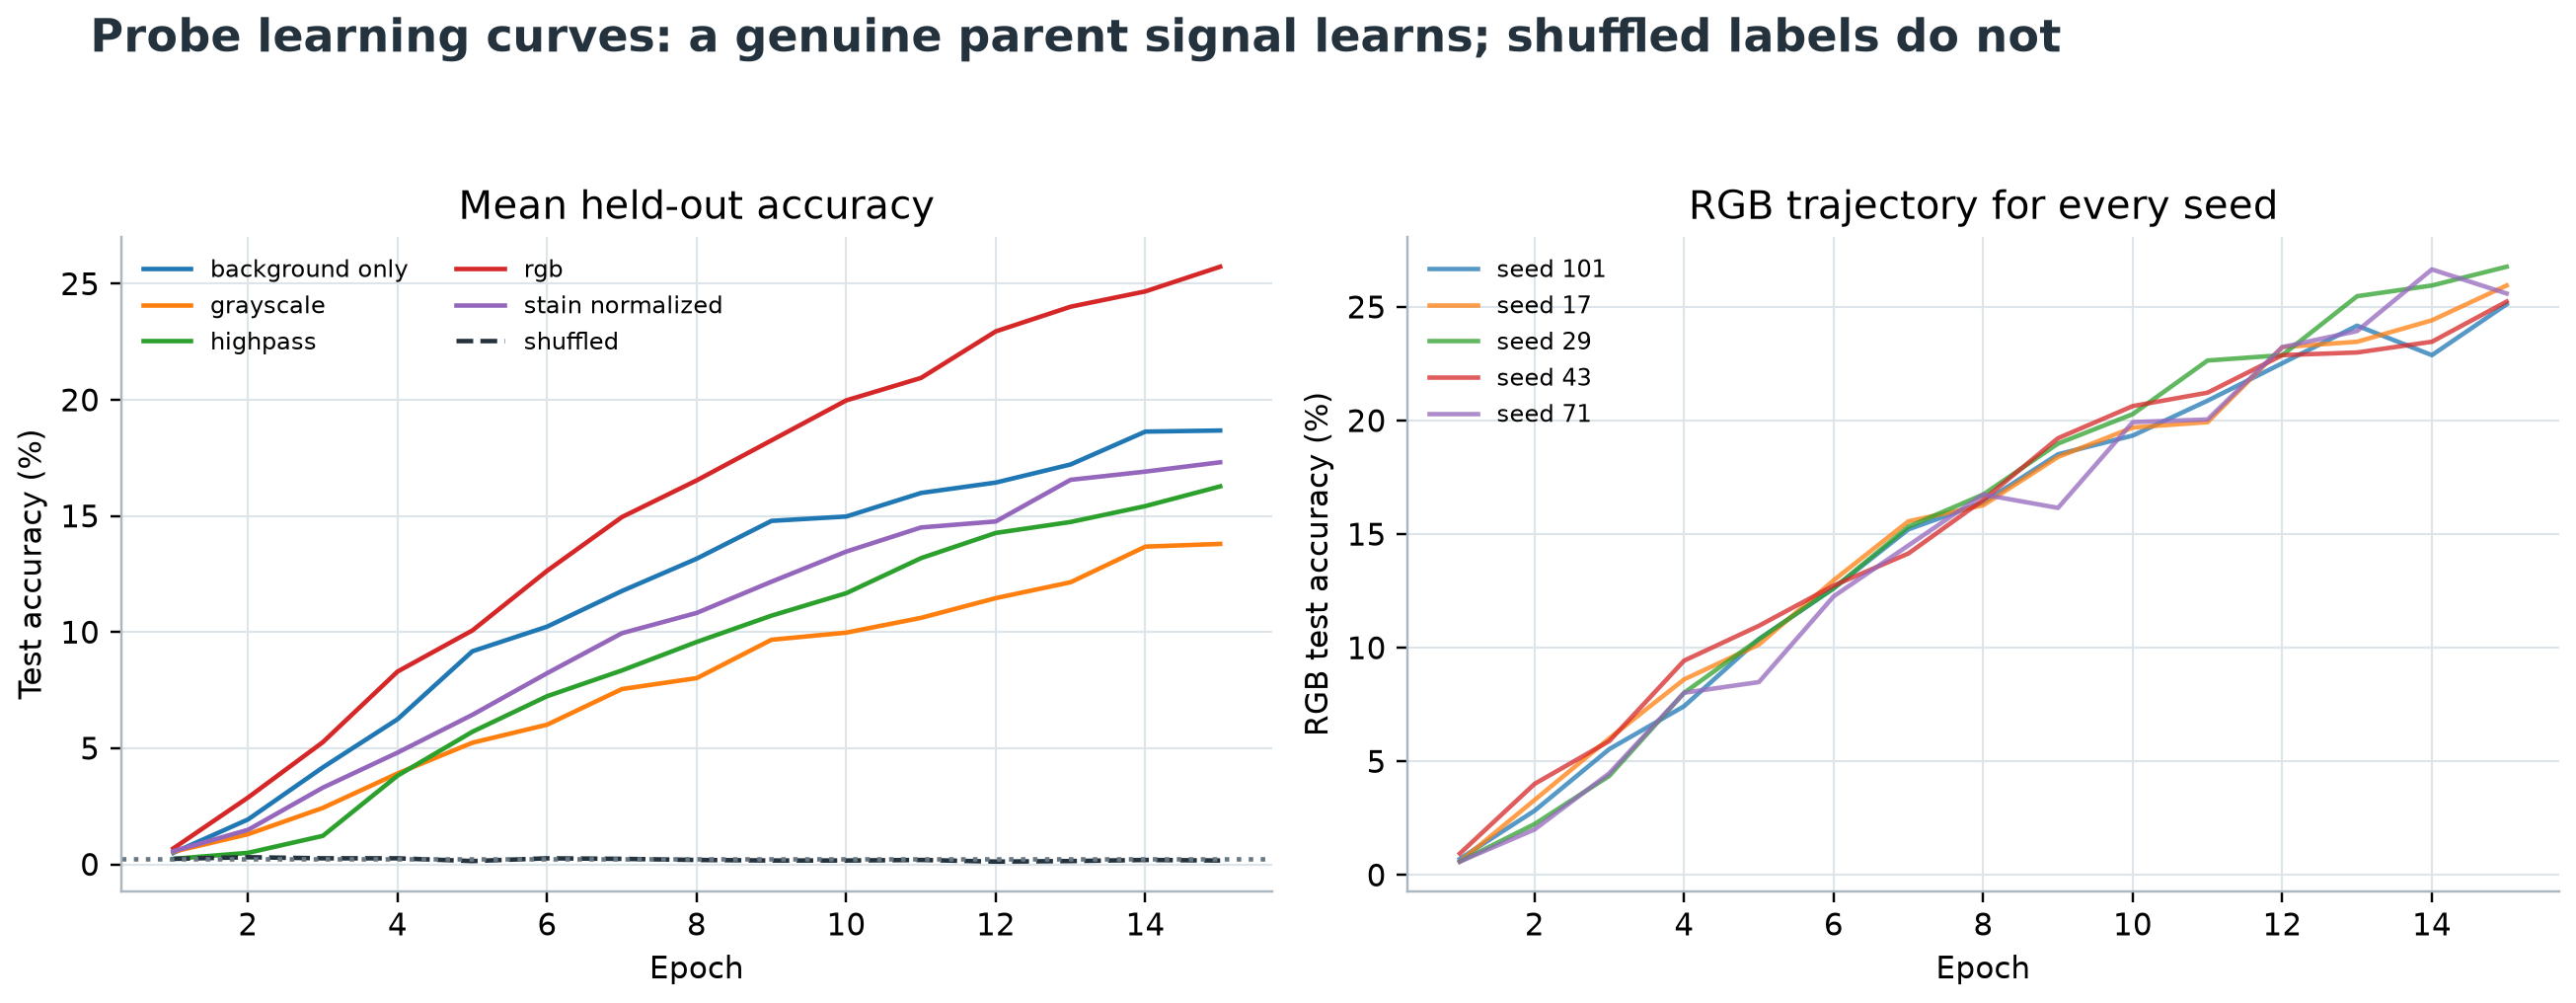
\includegraphics[width=\textwidth]{probe_learning_curves.png}
\caption{Probe learning curves reconstructed from every retained epoch history. The RGB signal rises smoothly across seeds; shuffled labels remain near chance.}
\label{s1:fig:probe-learning}
\end{figure}

The shuffled mean is 0.1651\%, SD 0.2445 percentage points, with a five-seed interval from $-0.1385$\% to 0.4687\%; the exact 0.2358\% chance value lies inside. A negative lower confidence limit is an ordinary symmetric small-sample interval artifact and does not imply negative accuracy.

Background-only accuracy is higher than grayscale and stain-normalized accuracy. That does not mean background is the only cue: RGB remains highest, and transformations alter multiple image properties at once. The careful conclusion is that parent information is distributed across color, low- and high-frequency structure, and background.

% Carried over verbatim from monograph/main.tex (Study 1 record, 13 Sep 2026).
\chapter{SIPaKMeD classification rescore}\label{s1:ch:ch10_sipakmed_classification_rescore}

\section{Why re-run models rather than quote published scores?}

Published numbers are entangled with architectures, preprocessing, augmentations, and---most importantly---different splits. Quoting them would not isolate the quantity of interest. The rescore therefore trains six representative image classifiers under the same code path, preprocessing, optimizer family, epoch budget, seeds, and four fixed split protocols. The only intended change across protocols is the independence constraint and, for the explicitly size-matched control, the number of retained training crops.

The six families cover different inductive biases and capacities: ResNet-18 and ResNet-50~\cite{he2016resnet}, DenseNet-121~\cite{huang2017densenet}, MobileNet-V2~\cite{sandler2018mobilenetv2}, EfficientNet-B0~\cite{tan2019efficientnet}, and ViT-B/16~\cite{dosovitskiy2021vit}. Each ImageNet-pretrained head is replaced with a five-way linear classifier. Re-running all six also prevents the conclusion from depending on one especially favorable architecture.

\section{Inputs, augmentation, and optimization}

Every crop is decoded as RGB, converted to a tensor, and normalized by the ImageNet channel statistics. Training augmentation consists of a random resized crop to $224\times224$ with scale in $[0.8,1.0]$, a horizontal flip, and a vertical flip. Test preprocessing is a deterministic resize to $224\times224$. The code records the fully resolved split hash and configuration beside every result.

All classifiers use AdamW~\cite{loshchilov2019adamw}, cross-entropy loss, and a fixed learning rate. The retained endpoint is the final epoch; there is no separate validation split or post-hoc best-epoch selection. A run is valid only when the stored identifiers match its split, the final file is complete, and all reported quantities are finite. Table~\ref{s1:tab:classifier-hparams} gives the execution contract.

\begin{table}[H]
\centering
\caption{SIPaKMeD classifier execution settings.}
\label{s1:tab:classifier-hparams}
\begin{tabular}{ll}
\toprule
Item & Setting \\
\midrule
Architectures & ResNet-18/50, DenseNet-121, MobileNet-V2, EfficientNet-B0, ViT-B/16 \\
Initialization & ImageNet pretrained \\
Input & RGB, $224\times224$ \\
Loss & Five-class cross entropy \\
Optimizer & AdamW \\
Learning rate & $10^{-4}$, fixed \\
Weight decay & $10^{-4}$ \\
Batch size & 64 \\
Epochs & 20, final-epoch endpoint \\
Seeds & 17, 29, 43, 71, 101 \\
Primary metric & Test accuracy \\
Hardware & NVIDIA RTX A6000; at most three concurrent GPU jobs \\
\bottomrule
\end{tabular}
\end{table}

\section{Metric definitions}

For true class $y_i$ and prediction $\hat y_i$, accuracy is
\begin{equation}
\operatorname{Acc}=\frac{1}{N}\sum_{i=1}^{N}\mathbf{1}\{\hat y_i=y_i\}.
\end{equation}
For class $c$, with precision $P_c$ and recall $R_c$,
\begin{equation}
F_{1,c}=\frac{2P_cR_c}{P_c+R_c},\qquad
F_{1,\mathrm{macro}}=\frac{1}{C}\sum_{c=1}^{C}F_{1,c}.
\end{equation}
Balanced accuracy is the unweighted mean class recall,
\begin{equation}
\operatorname{BAcc}=\frac{1}{C}\sum_{c=1}^{C}\frac{TP_c}{TP_c+FN_c}.
\end{equation}
The preregistered primary endpoint is accuracy. Macro-F1 and balanced accuracy check that the direction is not a class-frequency artifact; they are not used to shop for a smaller $p$-value.

\section{Aggregate scores}

\begin{table}[H]
\centering
\caption{SIPaKMeD test accuracy (\%), mean $\pm$ sample SD over five seeds. \protocol{P1$'$} is numerically identical to \protocol{P1} because the frozen stratified crop split already contained the registered 3,239 training and 810 test observations.}
\label{s1:tab:classification-main}
\small
\begin{tabular}{lrrrr}
\toprule
Architecture & \protocol{P1} & \protocol{P1$'$} & \protocol{P2} & \protocol{P3} \\
\midrule
DenseNet-121 & 98.12$\pm$0.28 & 98.12$\pm$0.28 & 96.72$\pm$0.69 & 97.38$\pm$0.50 \\
EfficientNet-B0 & 97.78$\pm$0.49 & 97.78$\pm$0.49 & 96.69$\pm$1.49 & 97.41$\pm$0.71 \\
MobileNet-V2 & 97.41$\pm$0.45 & 97.41$\pm$0.45 & 95.16$\pm$1.50 & 96.20$\pm$0.93 \\
ResNet-18 & 97.19$\pm$0.59 & 97.19$\pm$0.59 & 96.00$\pm$0.89 & 96.35$\pm$1.28 \\
ResNet-50 & 97.51$\pm$0.47 & 97.51$\pm$0.47 & 96.79$\pm$0.42 & 96.27$\pm$0.53 \\
ViT-B/16 & 97.14$\pm$0.95 & 97.14$\pm$0.95 & 95.56$\pm$0.84 & 95.53$\pm$1.68 \\
\bottomrule
\end{tabular}
\end{table}

\begin{figure}[H]
\centering
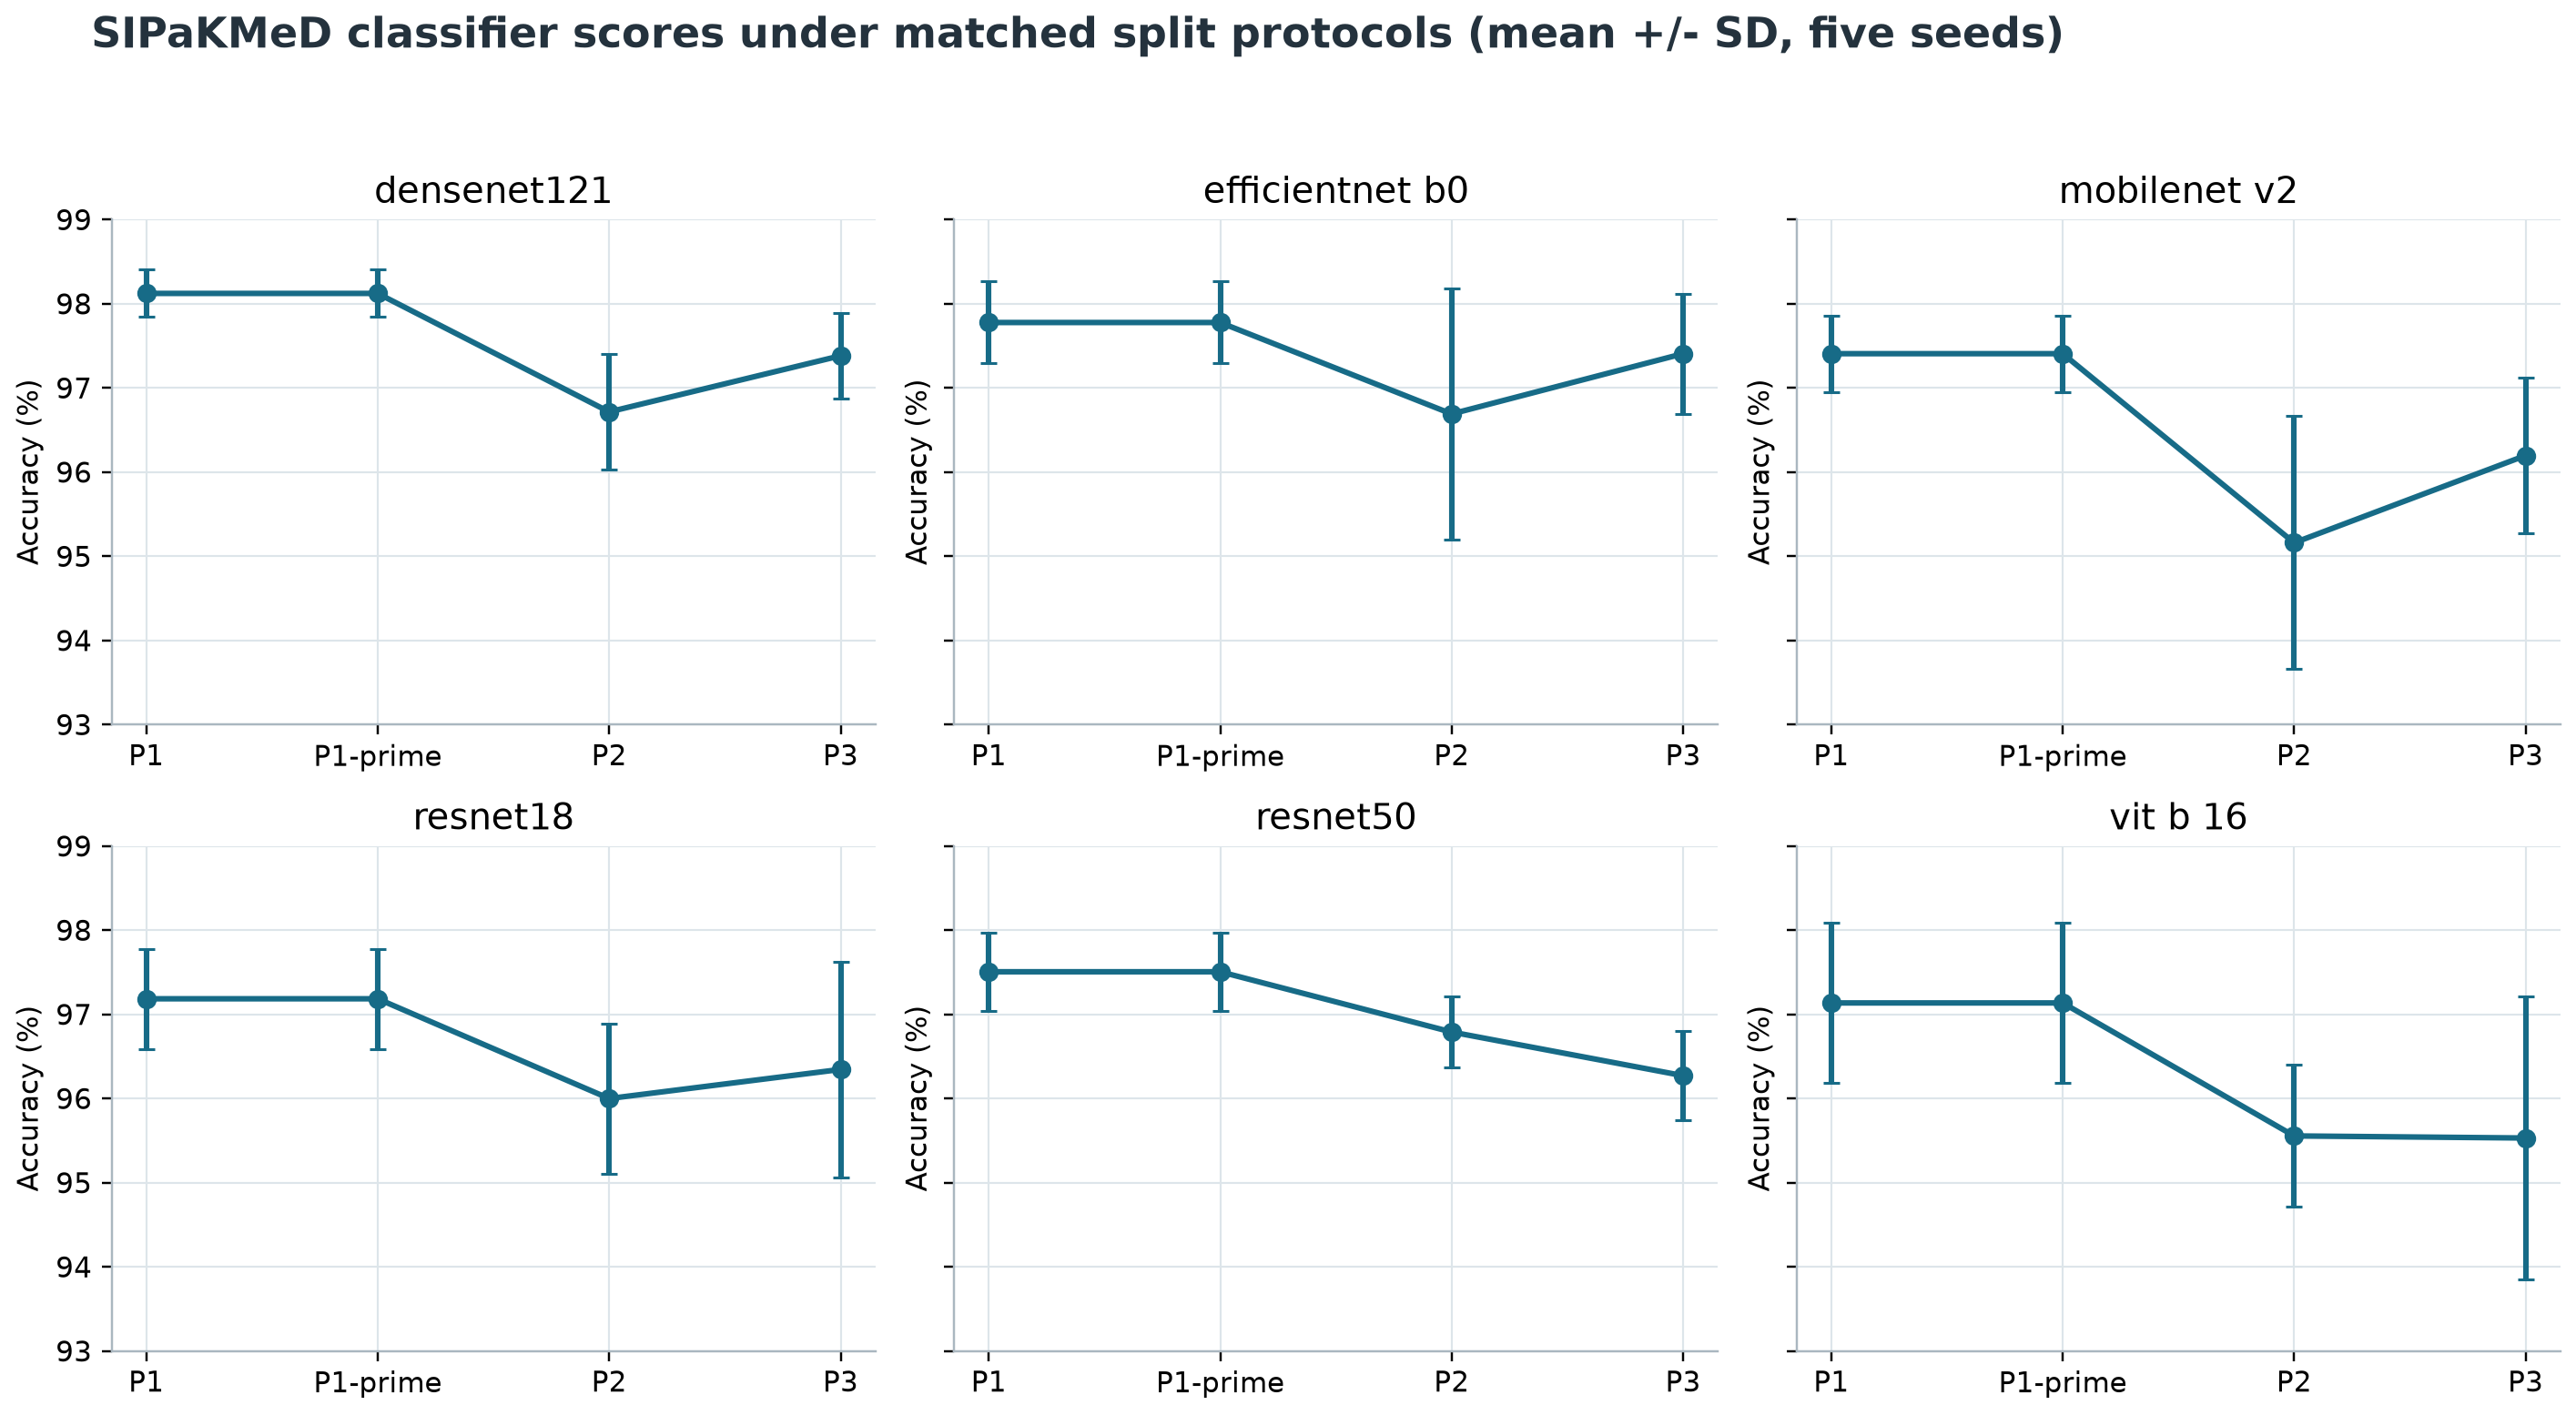
\includegraphics[width=\textwidth]{classification_protocol_scores.png}
\caption{All frozen SIPaKMeD accuracy observations. Lines connect the same architecture across protocols; points show individual seeds and bars show the mean.}
\label{s1:fig:classification-scores}
\end{figure}

The top score under \protocol{P1} is DenseNet-121 at 98.12$\pm$0.28\%. Under parent-disjoint \protocol{P2}, DenseNet-121 remains highest at 96.72$\pm$0.69\%, narrowly followed by ResNet-50. The key scientific observation is not which backbone wins; it is that all six paired \protocol{P1}$-$\protocol{P2} mean differences are positive.

\section{Matched contrasts, uncertainty, and the ordering failure}

For architecture $a$ and seed $s$, the primary paired difference is
\begin{equation}
d_{a,s}=100\left(\operatorname{Acc}_{a,s,\mathrm{P1}}-
\operatorname{Acc}_{a,s,\mathrm{P2}}\right)
\end{equation}
in percentage points. The paired standardized effect is Cohen's
\begin{equation}
d_z=\frac{\bar d}{s_d},
\end{equation}
where $s_d$ is the sample SD of the five seed-paired differences. Reported effect-size confidence intervals are seed-paired bootstrap intervals, so a bootstrap resample always keeps the two protocol results from a seed together. The test is a paired $t$-test because every registered five-difference vector passed its Shapiro--Wilk screen; the switch to Wilcoxon was reserved for a failed screen.

\begin{table}[H]
\centering
\caption{Primary SIPaKMeD \protocol{P1}$-$\protocol{P2} contrasts. The six paired $t$-tests form one preregistered BH family. CI is the paired-bootstrap 95\% interval for Cohen's $d_z$, not for the raw percentage-point mean.}
\label{s1:tab:classification-contrasts}
\small
\begin{tabular}{lrrrrr}
\toprule
Architecture & Mean$\pm$SD (pp) & 95\% CI for $d_z$ & $p$ & BH $q$ & $d_z$ \\
\midrule
DenseNet-121 & 1.41$\pm$0.90 & [0.985, 4.747] & 0.0251 & 0.1109 & 1.561 \\
EfficientNet-B0 & 1.09$\pm$1.85 & [$-$0.316, 4.668] & 0.2591 & 0.2591 & 0.588 \\
MobileNet-V2 & 2.25$\pm$1.63 & [0.809, 6.686] & 0.0370 & 0.1109 & 1.377 \\
ResNet-18 & 1.19$\pm$1.28 & [0.442, 2.365] & 0.1081 & 0.1511 & 0.922 \\
ResNet-50 & 0.72$\pm$0.83 & [0.085, 4.025] & 0.1260 & 0.1511 & 0.863 \\
ViT-B/16 & 1.58$\pm$1.70 & [0.057, 4.950] & 0.1059 & 0.1511 & 0.931 \\
\bottomrule
\end{tabular}
\end{table}

\begin{figure}[H]
\centering
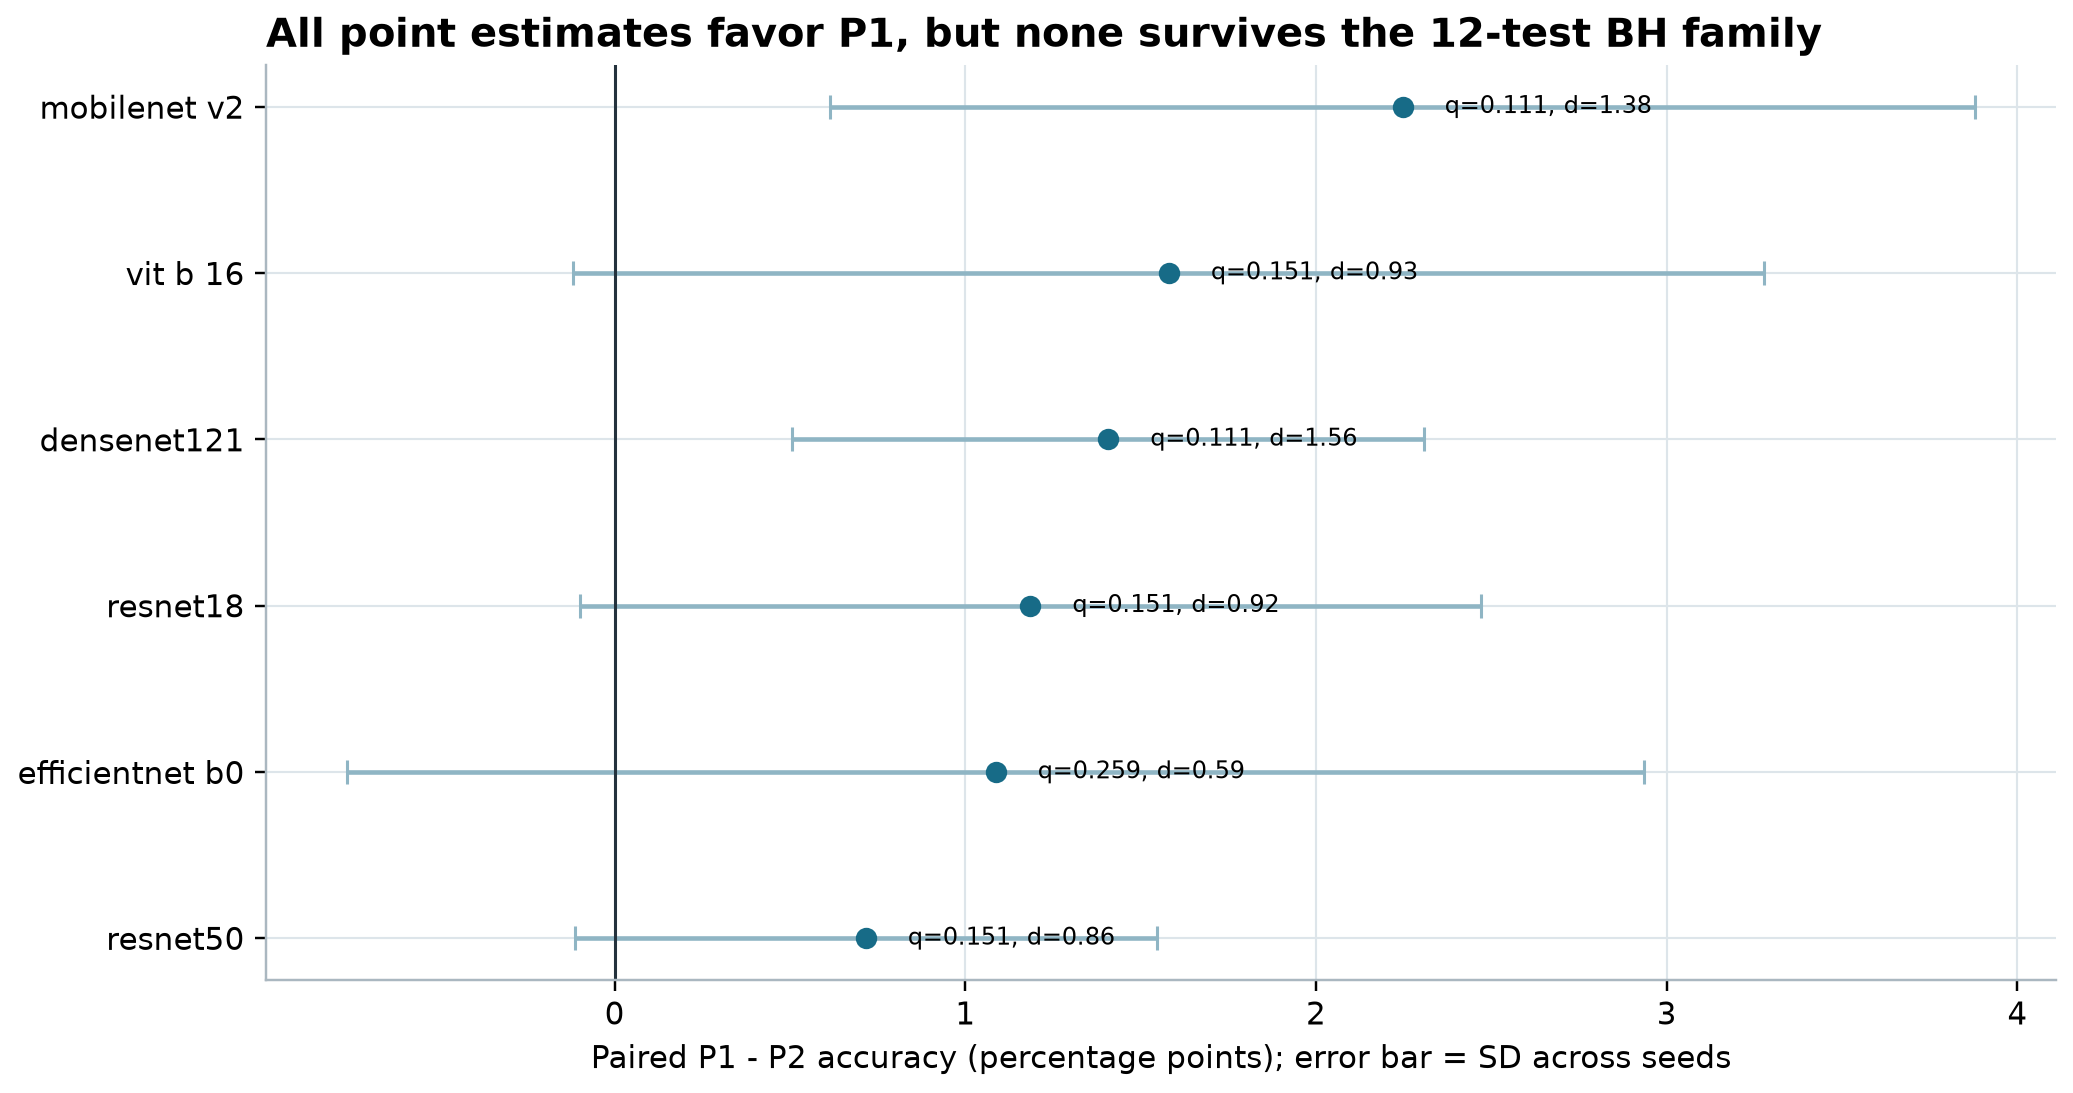
\includegraphics[width=\textwidth]{classification_delta_forest.png}
\caption{Paired \protocol{P1}$-$\protocol{P2} effects. Every mean favors the crop-level split, but none survives its preregistered multiplicity correction. The vertical line at zero marks no protocol effect.}
\label{s1:fig:classification-forest}
\end{figure}

\begin{figure}[H]
\centering
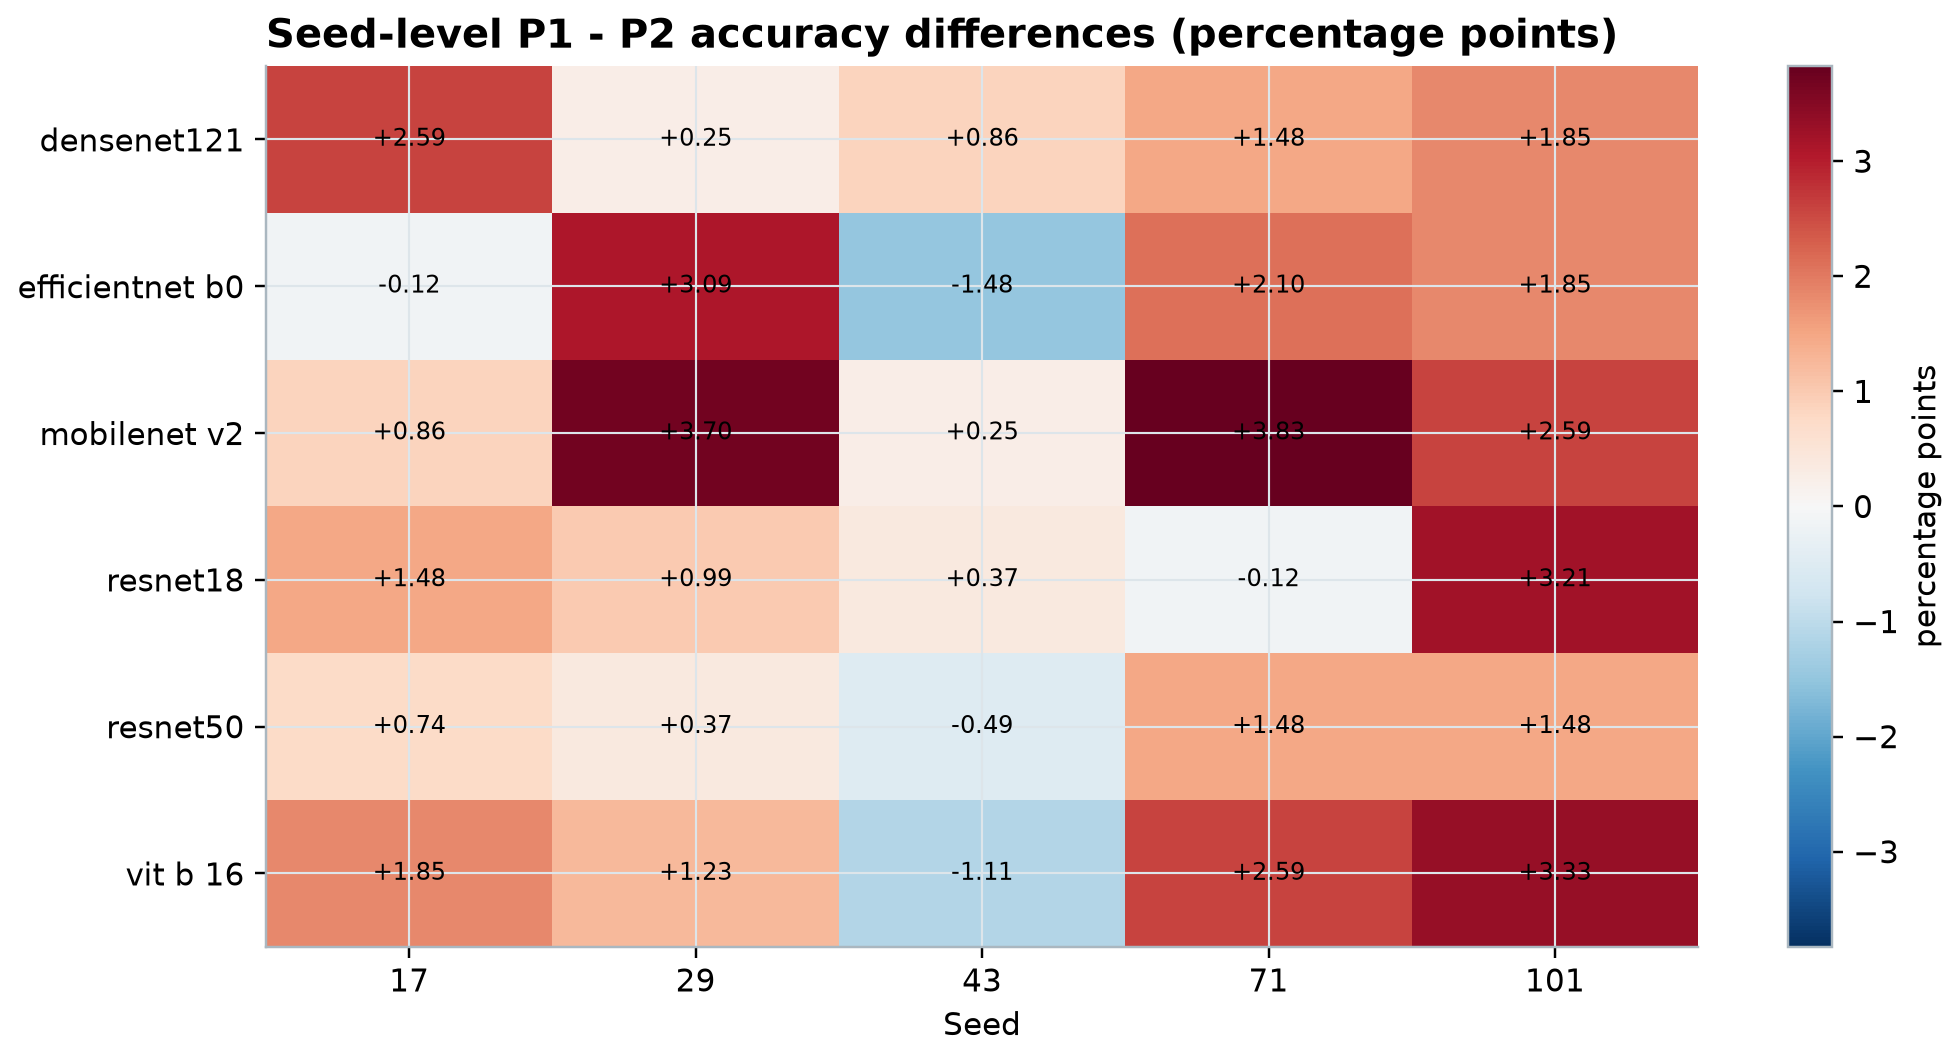
\includegraphics[width=\textwidth]{classification_seed_deltas.png}
\caption{Seed-level paired differences. This figure exposes the small effective sample size and the architecture-specific variability that an aggregate table can hide.}
\label{s1:fig:classification-seeds}
\end{figure}

The registered monotonicity expectation was \protocol{P3}$\leq$\protocol{P2}$\leq$\protocol{P1}. Only ResNet-50 and ViT-B/16 satisfy it. The other four improve from \protocol{P2} to \protocol{P3} by 0.35--1.04 points. Those reversals are not deleted or relabeled: the corresponding \protocol{P2}$-$\protocol{P3} differences are $-0.67$, $-0.72$, $-1.04$, $-0.35$, $+0.52$, and $+0.02$ points in table order, and none has an adjusted confirmatory claim.

\begin{figure}[H]
\centering
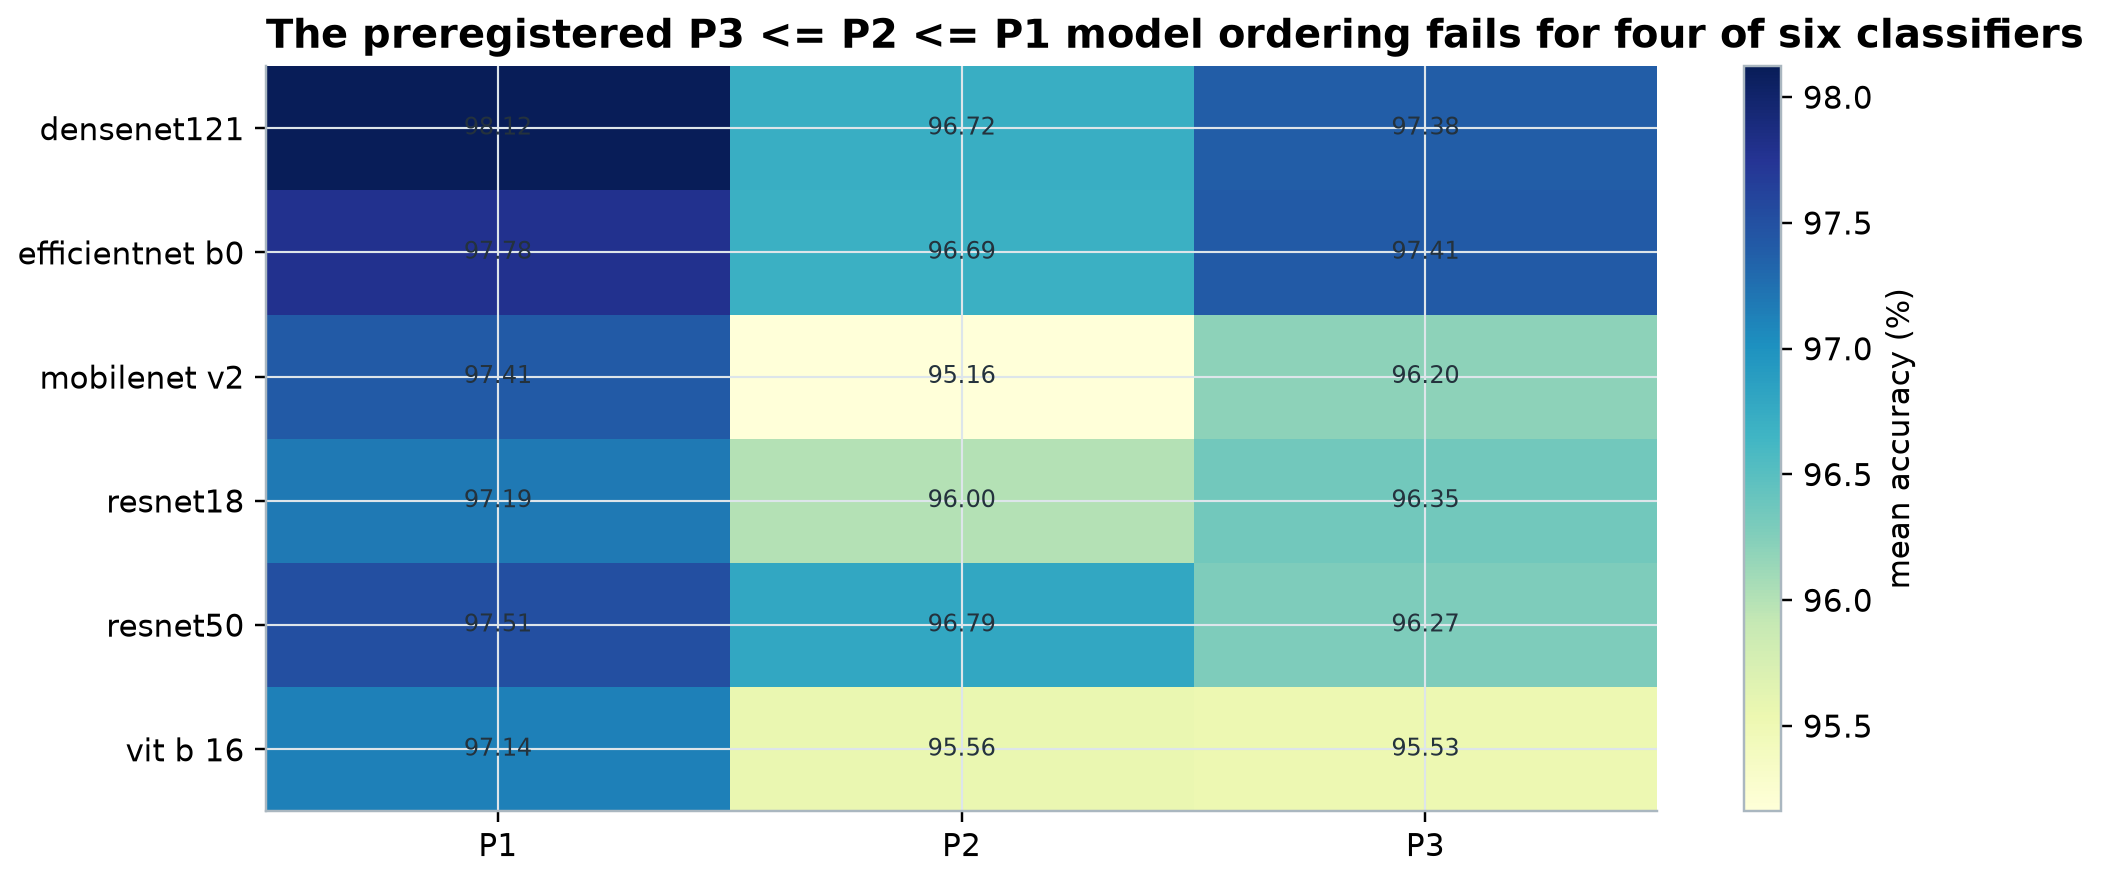
\includegraphics[width=\textwidth]{classification_ordering.png}
\caption{The registered ordering check. Cell values are the protocol means; the title records the gate outcome. Four of six architectures fail \protocol{P3}$\leq$\protocol{P2}$\leq$\protocol{P1}, so the acceptance contract correctly records one failed gate.}
\label{s1:fig:classification-ordering}
\end{figure}

Architecture ranks are also unstable across \protocol{P1} and \protocol{P2}: Kendall's $\tau=0.467$ with bootstrap interval [0.071, 0.733] and $p=0.2722$; four of the 15 architecture pairs reverse. This is a descriptive warning that a benchmark split can alter conclusions about model selection even when absolute score differences look modest.

\section{What the classification rescore does and does not show}

The same-sign result across six architectures is scientifically suggestive and consistent with the structural mechanism. The five-seed paired variability is nevertheless too large for any architecture to pass the six-test BH family. The correct report is therefore: \emph{crop-disjoint scores were higher on average for every tested classifier, by 0.72--2.25 percentage points, but the preregistered architecture-wise confirmatory family did not establish individual effects after multiplicity correction.}

No classifier confusion matrix appears because the frozen result schema retains aggregate test metrics and epoch histories, but not per-sample predictions or model checkpoints. Generating such a matrix now would require a new experiment after the declared research stop. Omitting it is more faithful than reconstructing or simulating unobserved cells.

\section{Training behavior and compute}

\begin{figure}[H]
\centering
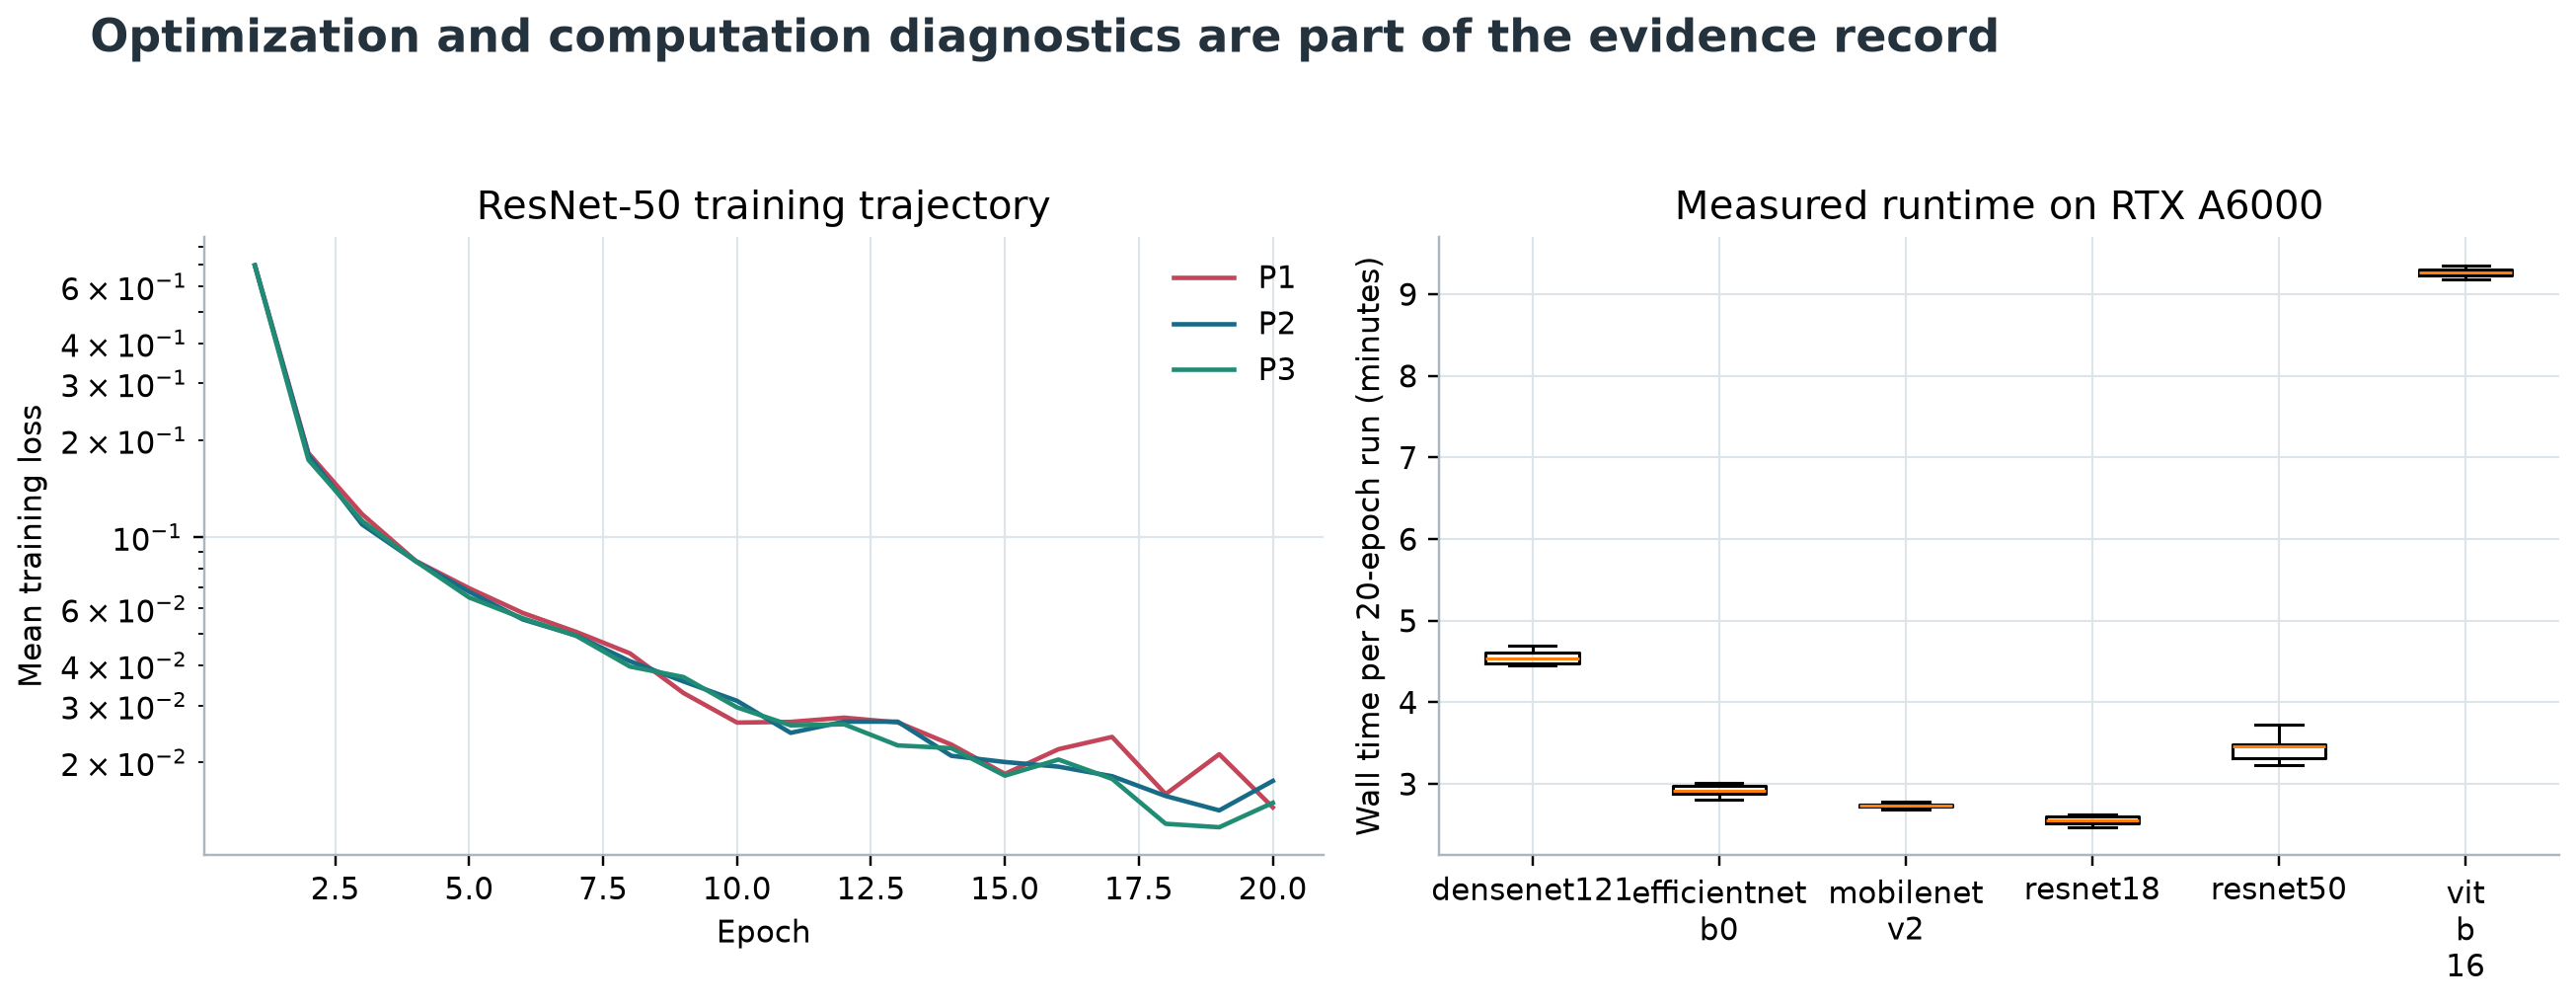
\includegraphics[width=\textwidth]{classification_training_runtime.png}
\caption{Classifier wall-clock summaries from the retained run JSON files. These are same-system measurements and should not be compared to timings reported on unrelated hardware.}
\label{s1:fig:classification-runtime}
\end{figure}

The 120 retained classification runs consumed 8.48 summed run-hours. Because up to three jobs ran concurrently, this is computational work, not elapsed calendar duration. Shorter wall time does not imply a more accurate or better-calibrated model; it is included so the execution cost is auditable.

% Carried over verbatim from monograph/main.tex (Study 1 record, 13 Sep 2026).
\chapter{Cx22 segmentation rescore}\label{s1:ch:ch11_cx22_segmentation_rescore}

\section{Why add a second task and dataset?}

Classification alone could leave two alternative explanations: perhaps the phenomenon is specific to SIPaKMeD, or perhaps it is specific to assigning a single label to a crop. Cx22 offers a different hierarchy and two pixel-level tasks. It therefore tests whether the split logic transfers to semantic and instance segmentation without pretending that its official split is the same estimand as the pooled stress test.

The pooled analysis treats all 1,320 released generated regions as the observation pool and the 514 CCEDD sources as parents. The protocol{OFFICIAL} arm uses only Cx22-Multi-Train (400 observations) and Cx22-Multi-Test (100 observations). These official train and test source-parent sets are disjoint. Pair is not added to the official test comparison: 55 of its source parents overlap Multi-Test and 233 overlap Multi-Train, with Jaccard similarities 0.126 and 0.475 respectively. Pooling and re-splitting is thus a downstream-reuse stress test, not an accusation that the authors' official Multi split is flawed.

\section{Targets and models}

The semantic target has two independent binary channels: cytoplasm and nucleus. Five encoder--decoder families are re-run: U-Net~\cite{ronneberger2015unet}, U-Net++~\cite{zhou2020unetplusplus}, DeepLabV3+~\cite{chen2018deeplabv3plus}, FPN~\cite{lin2017fpn}, and MAnet~\cite{fan2020manet}. ResNet-34 is the encoder except for DeepLabV3+, which uses ResNet-50. All encoders start from ImageNet weights. The output activation is not embedded in the network; logits are passed through sigmoid in the loss and evaluation code.

For image $i$, channel $c$, prediction probability $p_{icu}$, and binary target $y_{icu}$ at pixel $u$, the training objective is
\begin{align}
\mathcal L_{\mathrm{semantic}}
&=\mathcal L_{\mathrm{BCE}}+\mathcal L_{\mathrm{softDice}},\\
\mathcal L_{\mathrm{softDice}}
&=1-\frac{1}{2N}\sum_{i,c}
\frac{2\sum_u p_{icu}y_{icu}+1}
{\sum_u p_{icu}+\sum_u y_{icu}+1}.
\end{align}

The instance task uses Mask R-CNN with a ResNet-50 FPN backbone and its torchvision V2 implementation~\cite{he2017maskrcnn}. The classification and mask heads are replaced for one foreground category plus background. Ground-truth cytoplasm instances are reconstructed from the released MATLAB label structure before resizing. Empty instances after resizing are rejected rather than silently retained.

\section{Deterministic input construction}

All images and masks are resized to $256\times256$; RGB images use antialiased interpolation, while masks use nearest-neighbor interpolation. Training augmentation is determined by a SHA-256 digest of seed, epoch, and crop ID. Digest bits choose horizontal flip, vertical flip, and one of four right-angle rotations. This produces per-epoch augmentation without relying on worker scheduling order. Images are ImageNet-normalized; masks remain binary.

The original JPEGs and generated masks were packed into memory-mappable arrays, each named in a provenance manifest with SHA-256 hashes and a cache version. This was not a scientific transformation. It removed repeated JPEG/MATLAB/NFS decoding from the inner loop while making the exact input bytes auditable.

\begin{table}[H]
\centering
\caption{Cx22 segmentation execution settings.}
\label{s1:tab:cx22-hparams}
\begin{tabular}{lll}
\toprule
Item & Semantic & Instance \\
\midrule
Image size & $256\times256$ & $256\times256$ \\
Epochs & 30 & 30 \\
Batch size & 16 & 2 (test batch 1) \\
Optimizer & AdamW & AdamW \\
Learning rate & $10^{-4}$ fixed & $10^{-4}$ fixed \\
Weight decay & $10^{-4}$ & $10^{-4}$ \\
Precision & FP16 except MAnet FP32 & FP16 \\
Endpoint schedule & every epoch; final retained & final epoch only \\
Checkpointing & every epoch & every 5 epochs \\
Seeds & 17, 29, 43, 71, 101 & 17, 29, 43, 71, 101 \\
Hardware & \multicolumn{2}{l}{NVIDIA RTX A6000; at most three concurrent GPU jobs} \\
\bottomrule
\end{tabular}
\end{table}

\section{Semantic metrics}

Probabilities are thresholded at 0.5. For predicted set $A$ and target set $B$,
\begin{equation}
\operatorname{Dice}(A,B)=\frac{2|A\cap B|}{|A|+|B|},\qquad
\operatorname{IoU}(A,B)=\frac{|A\cap B|}{|A\cup B|}.
\end{equation}
The primary semantic value first averages cytoplasm and nucleus Dice within each image, then averages over test images. This prevents a large cytoplasm region from numerically drowning the smaller nucleus. Channel-specific Dice and IoU are retained as diagnostic endpoints.

\section{Instance matching metric}

Predictions with object score below 0.5 are discarded. Let $D_{jk}$ be Dice between predicted instance $j$ and ground-truth instance $k$. The Hungarian assignment~\cite{kuhn1955hungarian} maximizes
\begin{equation}
\max_{\pi}\sum_{(j,k)\in\pi}D_{jk}
\end{equation}
subject to one-to-one matching. Every unmatched ground-truth instance receives Dice and IoU zero. The primary image value is the mean over that image's ground-truth instances; images are then averaged. Recall@0.70 is the fraction of ground-truth instances whose matched Dice is at least 0.70. This endpoint penalizes missed cells and does not allow an image with many easy instances to dominate the result.

\begin{lstlisting}[style=cyto,caption={Exact logic of the matched-instance endpoint.},label={lst:instance-metric}]
keep predictions with confidence >= 0.50
threshold predicted and target masks at 0.50
compute all predicted-by-target Dice values on the GPU
solve maximum-weight one-to-one assignment
write matched Dice into a zero vector of length n_targets
average the vector within the image
average image means over the test set
\end{lstlisting}

\section{Semantic results}

\begin{table}[H]
\centering
\caption{Cx22 semantic macro-Dice (\%), mean $\pm$ sample SD over five seeds. The official column uses a different 400/100 sample and is descriptive, not a paired protocol contrast.}
\label{s1:tab:cx22-semantic}
\small
\begin{tabular}{lrrrrr}
\toprule
Model & \protocol{P1} & \protocol{P1$'$} & \protocol{P2} & \protocol{P3} & \protocol{OFFICIAL} \\
\midrule
DeepLabV3+ & 88.90$\pm$0.45 & 88.84$\pm$0.45 & 88.64$\pm$0.34 & 88.10$\pm$0.38 & 82.96$\pm$1.54 \\
FPN & 88.90$\pm$0.43 & 88.97$\pm$0.55 & 88.89$\pm$0.48 & 88.33$\pm$0.30 & 84.43$\pm$0.33 \\
MAnet & 90.03$\pm$0.60 & 90.07$\pm$0.63 & 89.97$\pm$0.45 & 89.63$\pm$0.21 & 85.50$\pm$1.41 \\
U-Net & 90.29$\pm$0.48 & 90.32$\pm$0.52 & 89.99$\pm$0.52 & 89.77$\pm$0.16 & 85.64$\pm$0.58 \\
U-Net++ & 90.56$\pm$0.51 & 90.58$\pm$0.54 & 90.38$\pm$0.35 & 90.05$\pm$0.21 & 87.30$\pm$1.13 \\
\bottomrule
\end{tabular}
\end{table}

\begin{figure}[H]
\centering
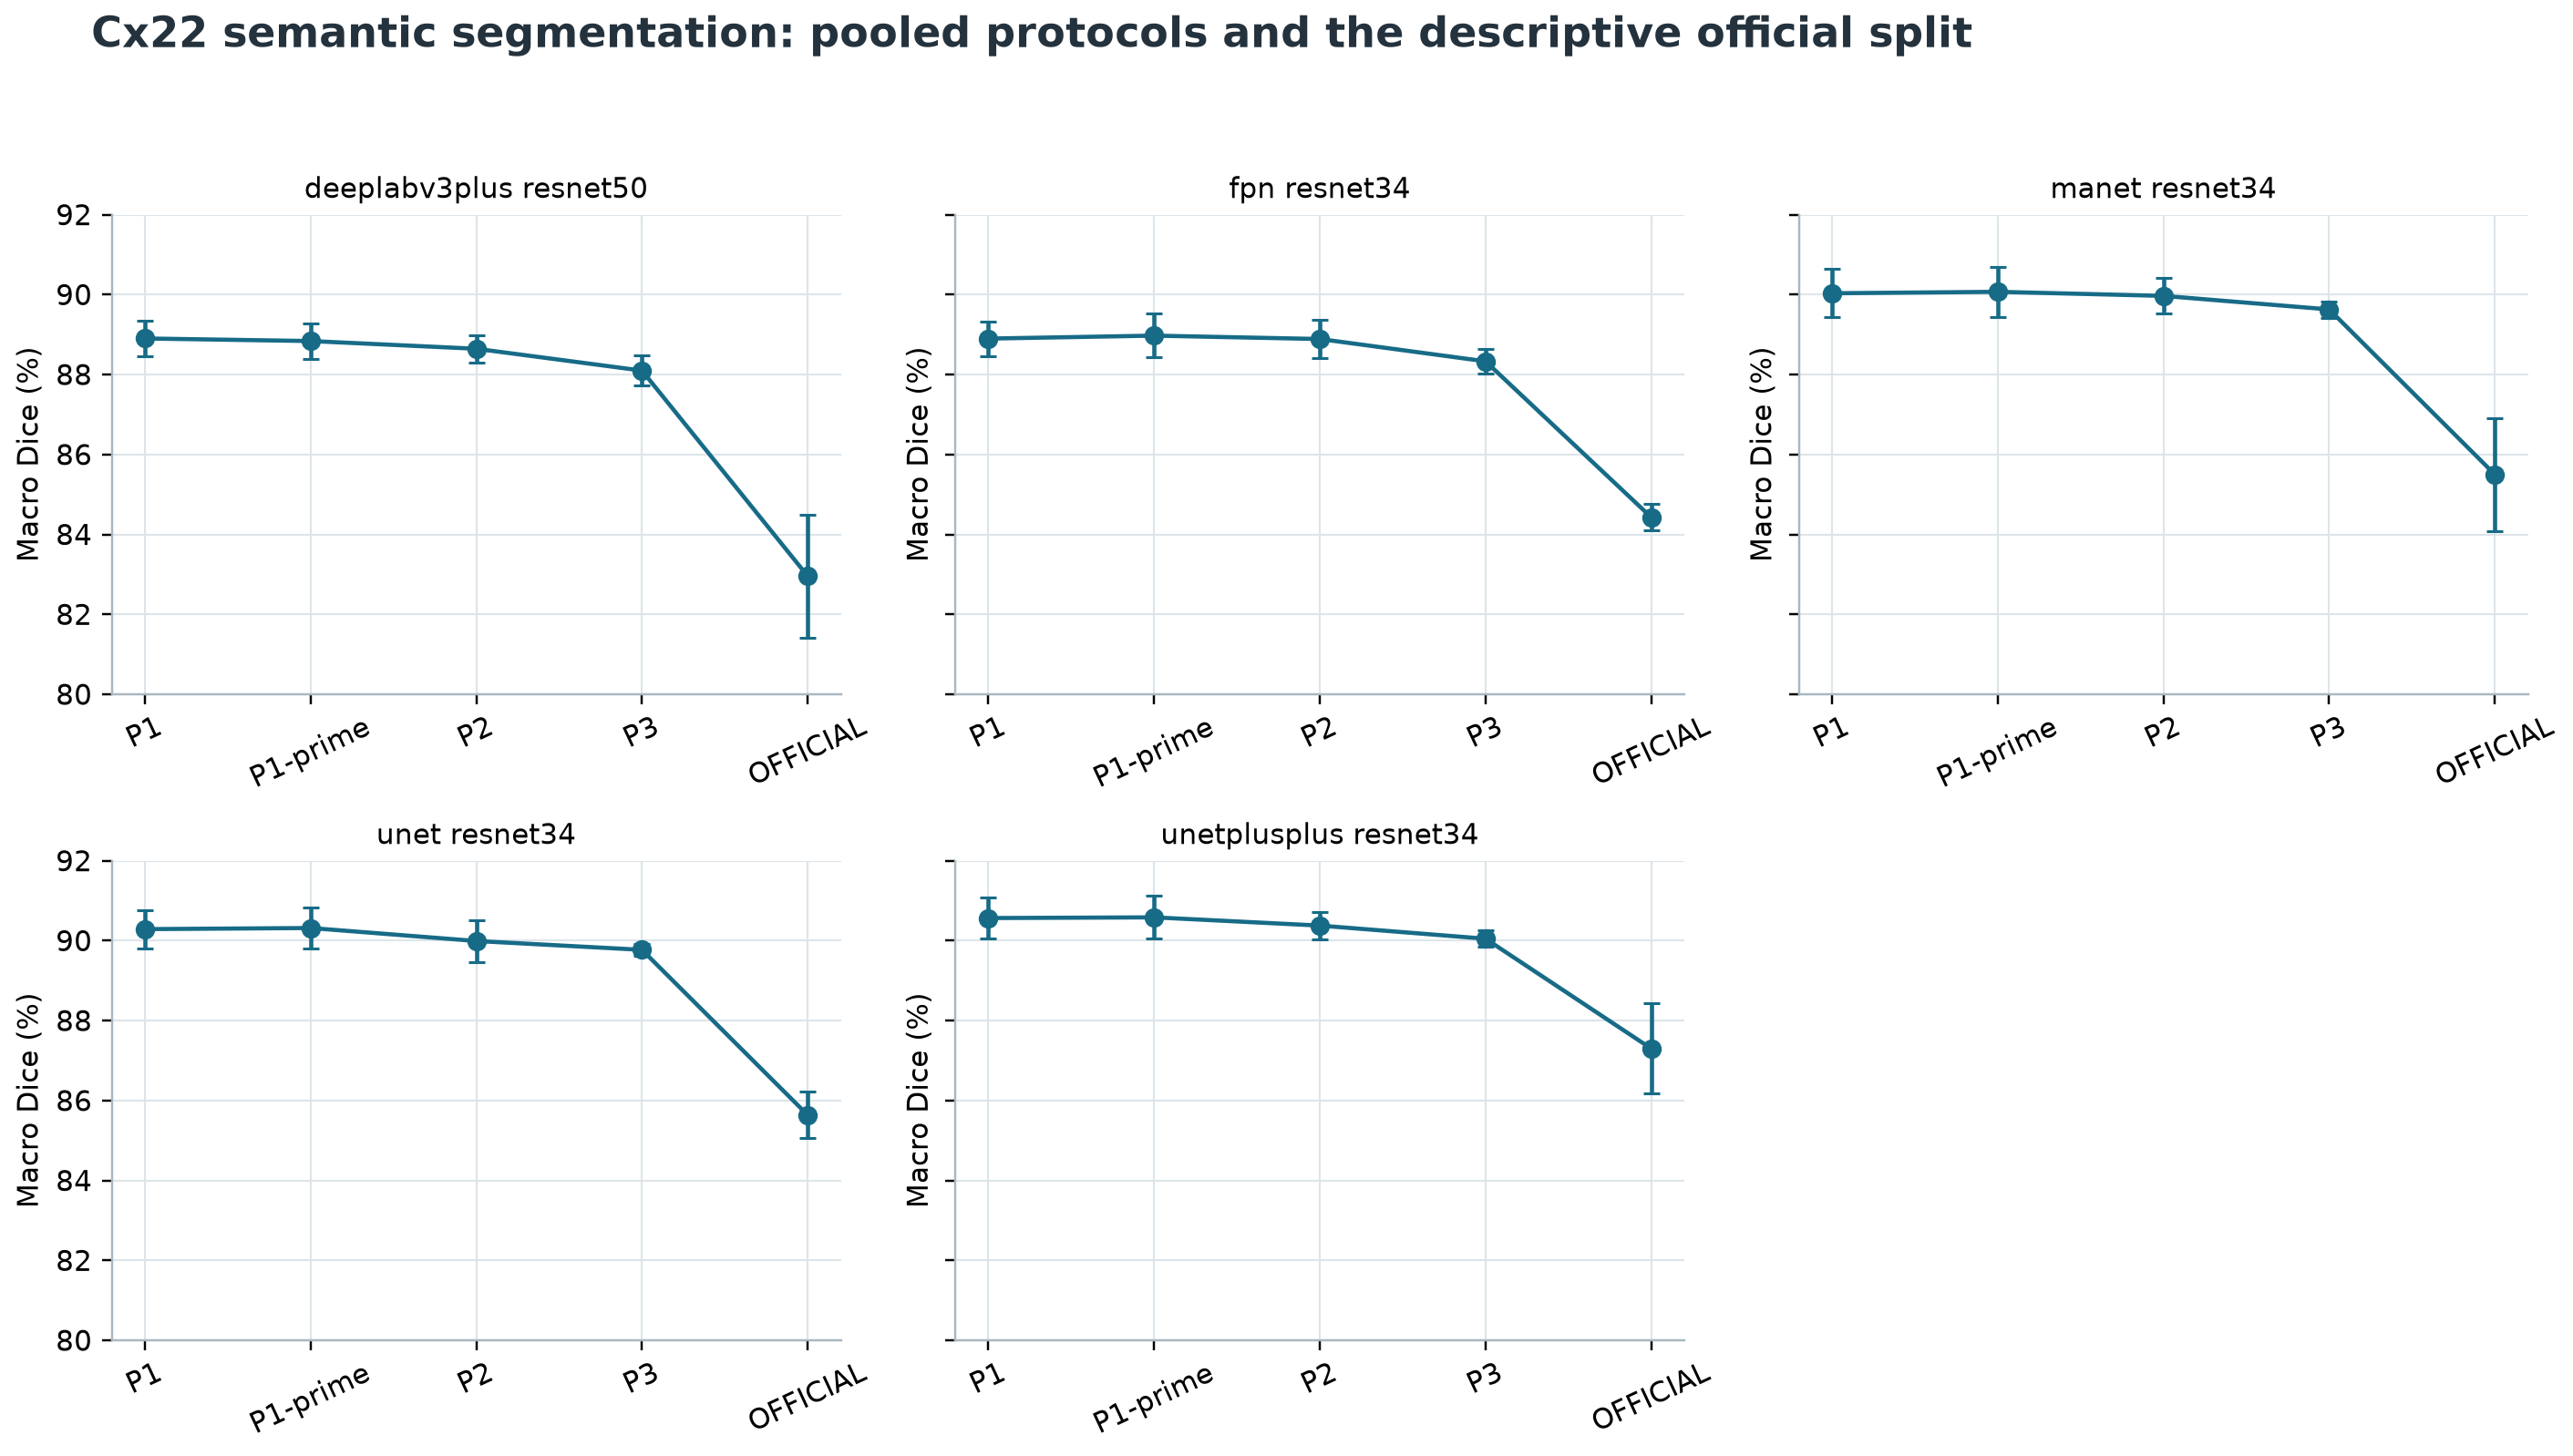
\includegraphics[width=\textwidth]{cx22_semantic_scores.png}
\caption{Cx22 semantic macro-Dice by architecture and protocol. The official arm is visually separated because it is not a same-observation contrast.}
\label{s1:fig:cx22-semantic}
\end{figure}

\begin{figure}[H]
\centering
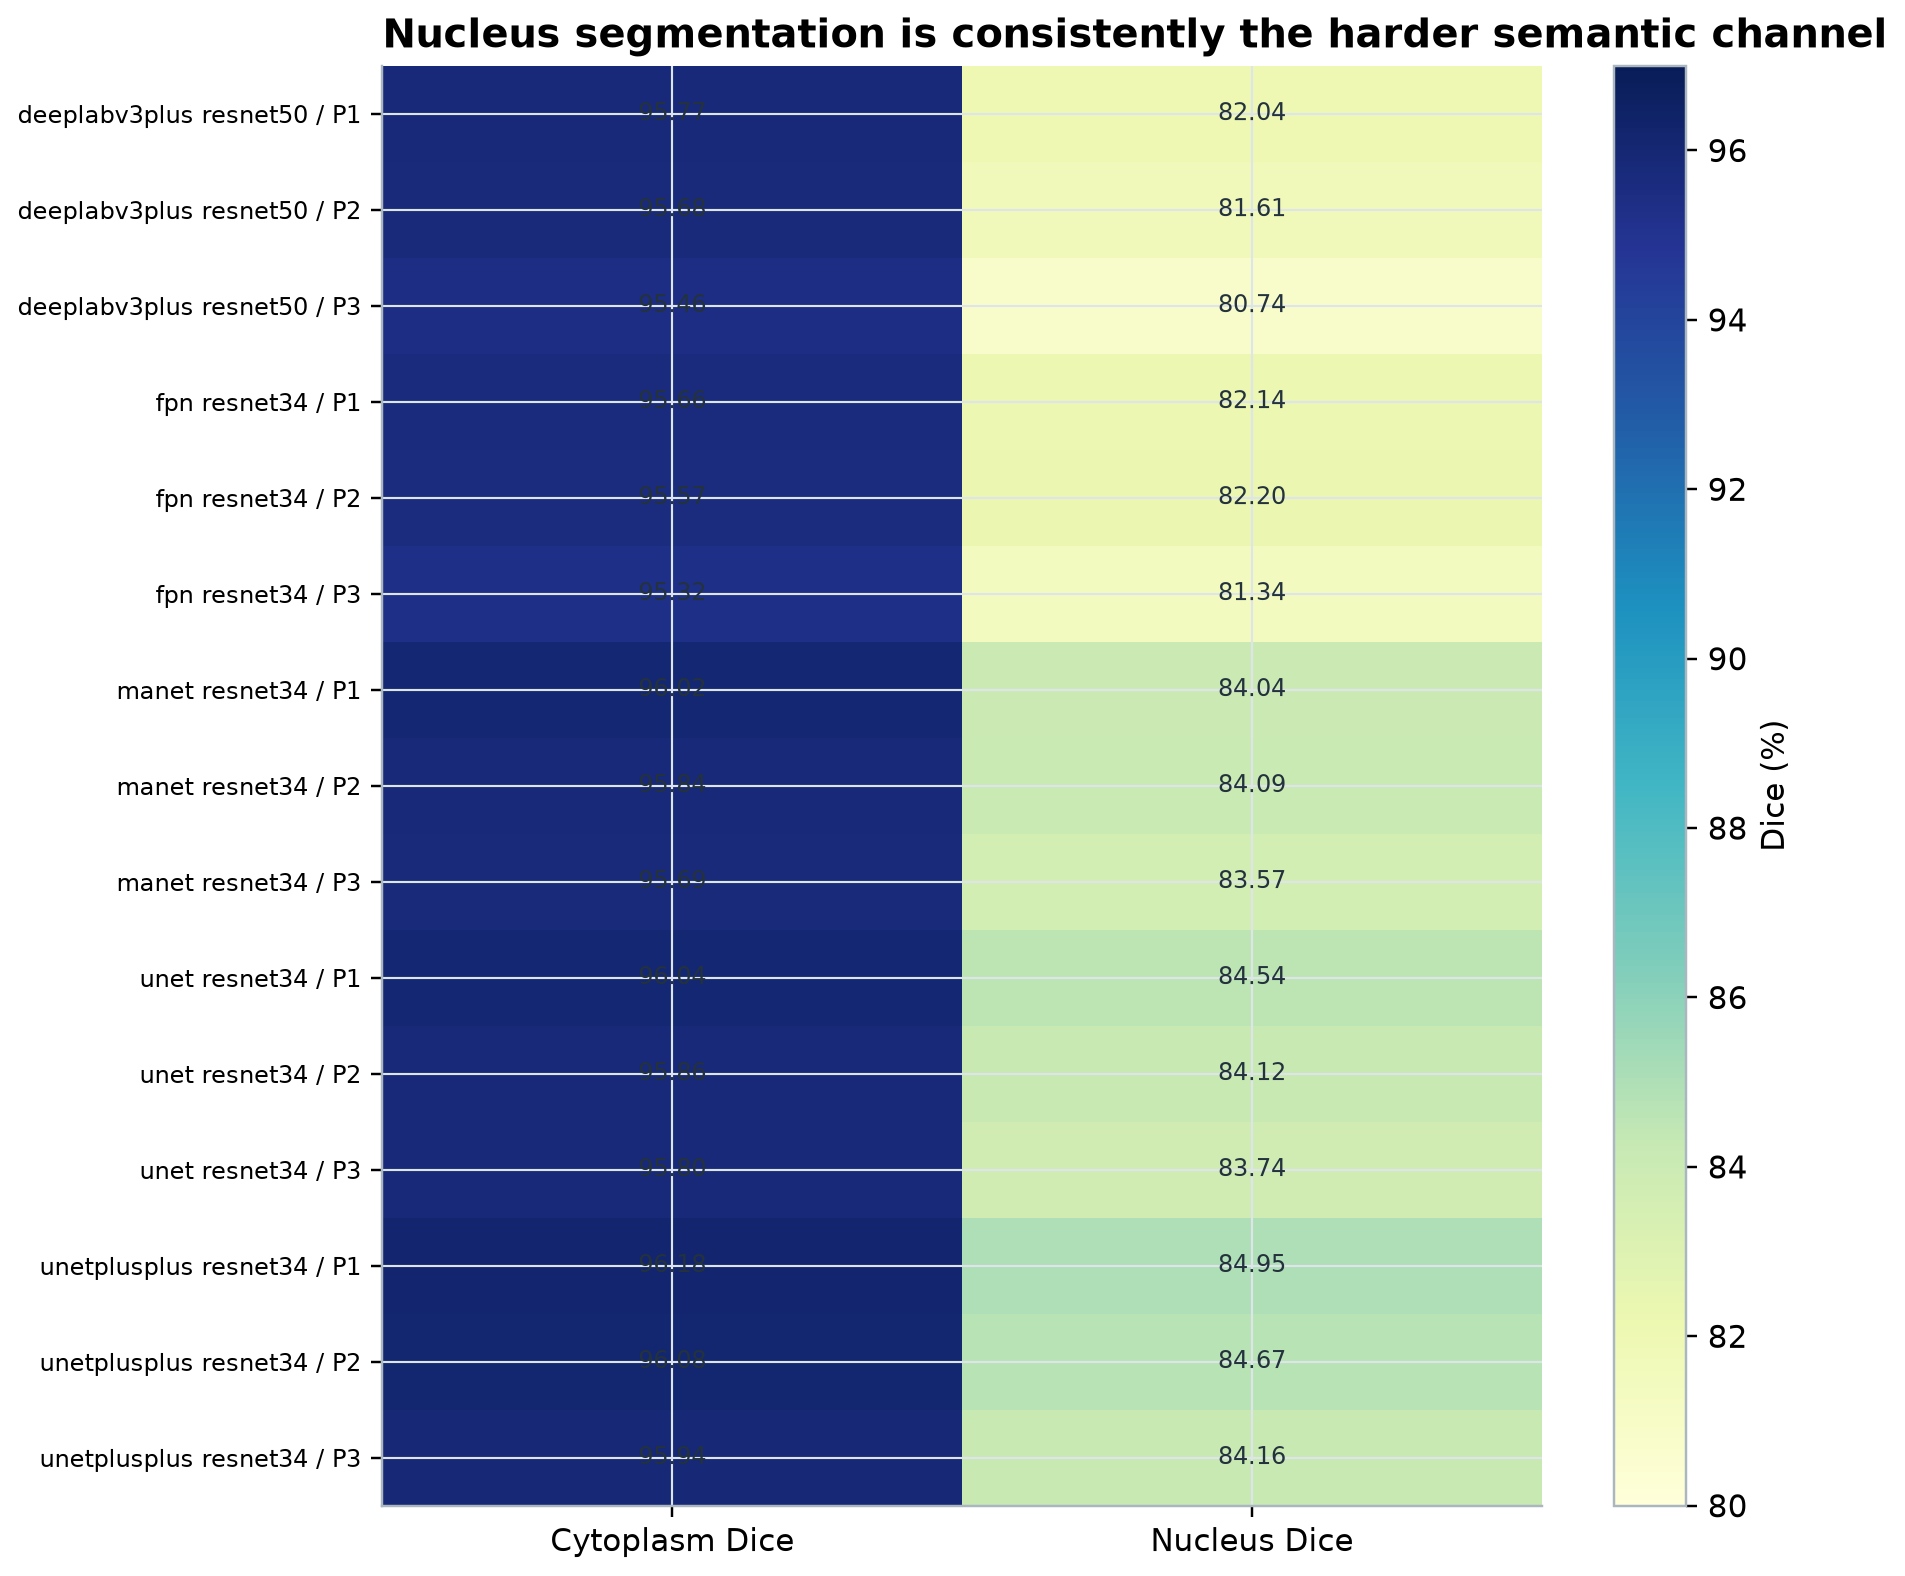
\includegraphics[width=\textwidth]{cx22_channel_heatmap.png}
\caption{Channel-level Dice makes the central difficulty visible: nuclei are consistently harder than cytoplasm. This is the segmentation analogue of a confusion-matrix diagnostic and uses retained aggregate channel measurements, not invented pixel predictions.}
\label{s1:fig:cx22-channels}
\end{figure}

U-Net++ is best in every pooled protocol and on the official Multi arm. The channel breakdown explains the lower official macro score: across models, cytoplasm Dice is roughly 94--95\% while nucleus Dice is roughly 72--79\%. Nuclei are smaller, so a fixed boundary displacement consumes a larger fraction of their area; faint staining and overlap also make the boundary less stable. This is a checkable data property visible in the released masks rather than a generic explanation added after the fact.

\section{Instance results}

\begin{table}[H]
\centering
\caption{Cx22 matched-instance Dice (\%), mean $\pm$ sample SD over five seeds.}
\label{s1:tab:cx22-instance}
\small
\begin{tabular}{lrrrrr}
\toprule
Model & \protocol{P1} & \protocol{P1$'$} & \protocol{P2} & \protocol{P3} & \protocol{OFFICIAL} \\
\midrule
Mask R-CNN & 92.10$\pm$0.52 & 92.05$\pm$0.52 & 91.59$\pm$0.42 & 91.11$\pm$1.09 & 92.29$\pm$0.32 \\
Mask R-CNN V2 & 91.99$\pm$0.57 & 91.95$\pm$0.58 & 91.36$\pm$0.82 & 90.60$\pm$0.52 & 92.18$\pm$0.71 \\
\bottomrule
\end{tabular}
\end{table}

\begin{figure}[H]
\centering
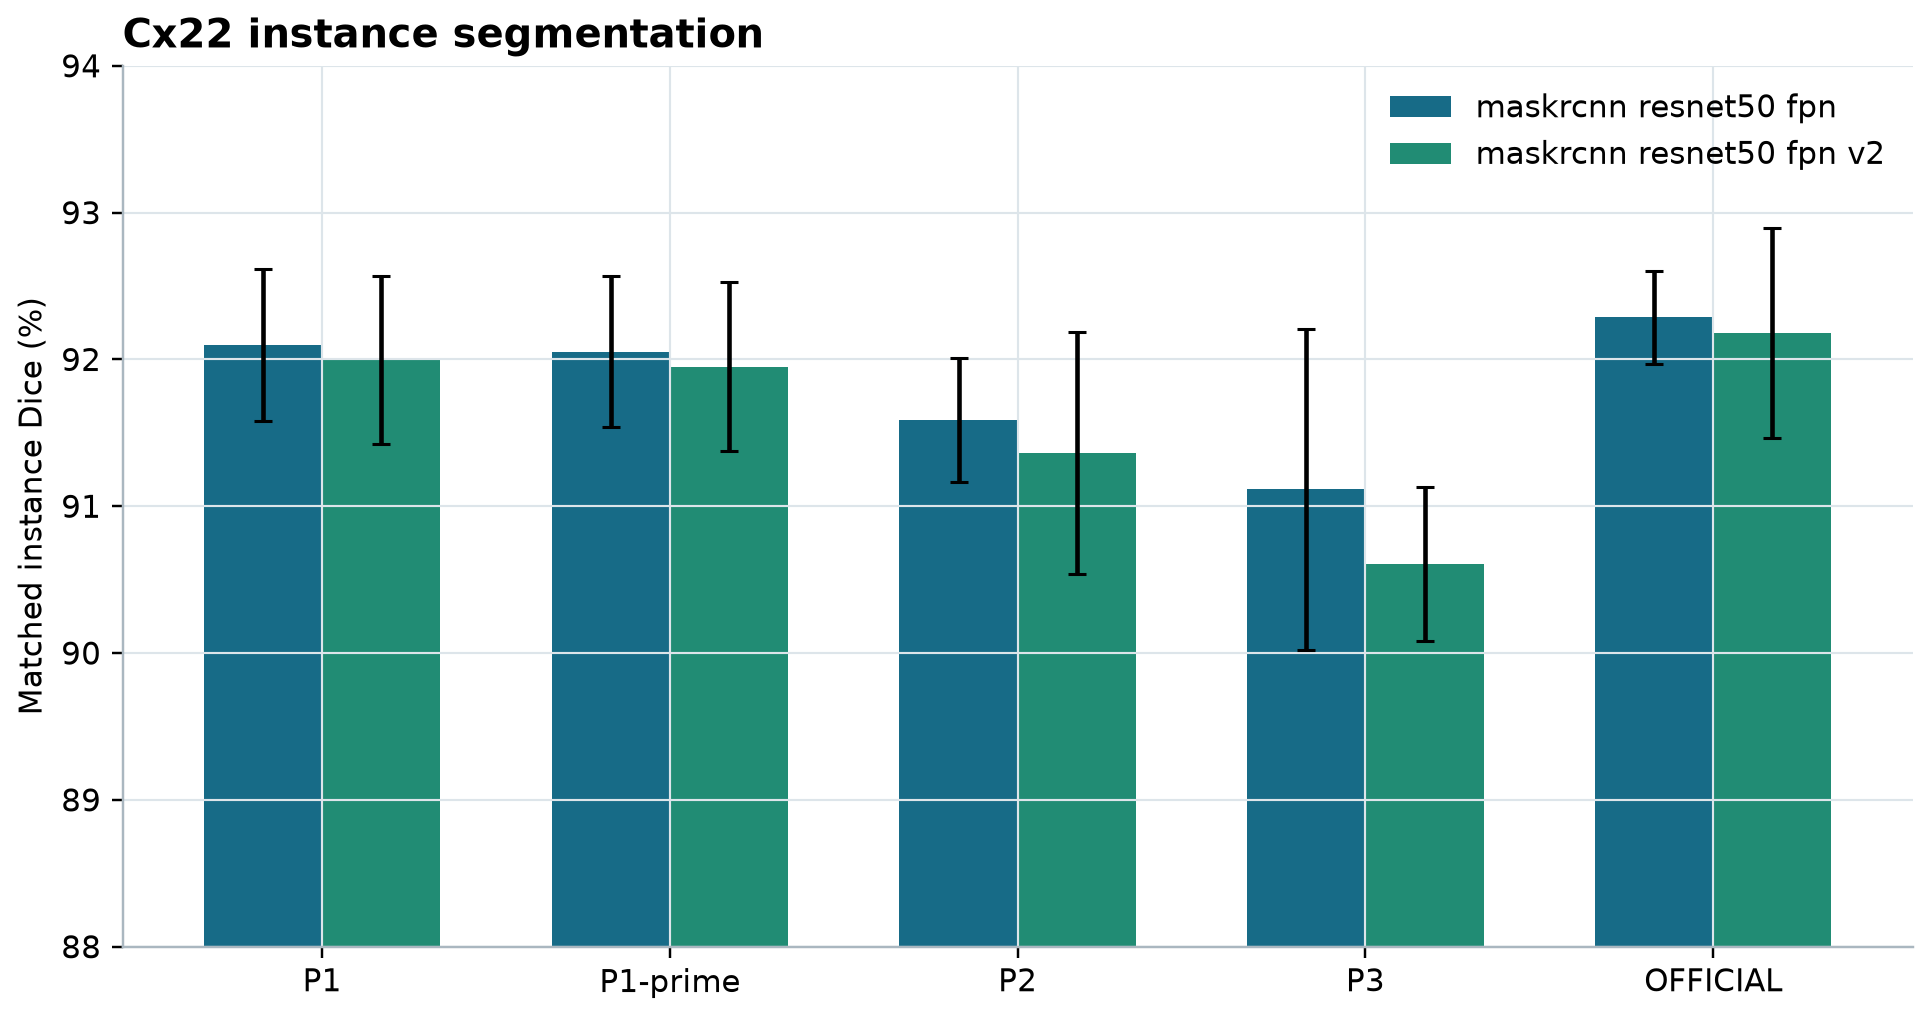
\includegraphics[width=\textwidth]{cx22_instance_scores.png}
\caption{Cx22 matched-instance Dice. Both Mask R-CNN variants follow the complete registered \protocol{P3}$\leq$\protocol{P2}$\leq$\protocol{P1} ordering.}
\label{s1:fig:cx22-instance}
\end{figure}

Unlike SIPaKMeD classification, all seven Cx22 architecture/task rows satisfy the registered ordering. The differences are still small: \protocol{P1}$-$\protocol{P2} is 0.01--0.30 percentage points for semantic models and 0.51--0.63 points for instance models.

\section{Inference and rank stability}

\begin{table}[H]
\centering
\caption{Primary Cx22 \protocol{P1}$-$\protocol{P2} contrasts. Values are mean $\pm$ SD percentage points; $q$ is within the task-specific preregistered family. Effect is Cohen's $d_z$ except DeepLabV3+, whose non-normal seed differences trigger rank-biserial effect size.}
\label{s1:tab:cx22-primary}
\small
\begin{tabular}{llrrrr}
\toprule
Task & Model & Mean$\pm$SD & Raw $p$ & BH $q$ & Effect \\
\midrule
Semantic & DeepLabV3+ & 0.258$\pm$0.418 & 0.3125 & 0.8458 & 0.600$^{\dagger}$ \\
Semantic & FPN & 0.010$\pm$0.468 & 0.9625 & 0.9625 & 0.022 \\
Semantic & MAnet & 0.065$\pm$0.450 & 0.7612 & 0.8458 & 0.146 \\
Semantic & U-Net & 0.297$\pm$0.767 & 0.4353 & 0.8458 & 0.387 \\
Semantic & U-Net++ & 0.188$\pm$0.406 & 0.3582 & 0.8458 & 0.464 \\
Instance & Mask R-CNN & 0.509$\pm$0.581 & 0.1220 & 0.2440 & 0.875 \\
Instance & Mask R-CNN V2 & 0.630$\pm$1.204 & 0.3068 & 0.3116 & 0.523 \\
\bottomrule
\multicolumn{6}{l}{\footnotesize $^{\dagger}$rank-biserial correlation; all other effects are Cohen's $d_z$.}
\end{tabular}
\end{table}

\begin{figure}[H]
\centering
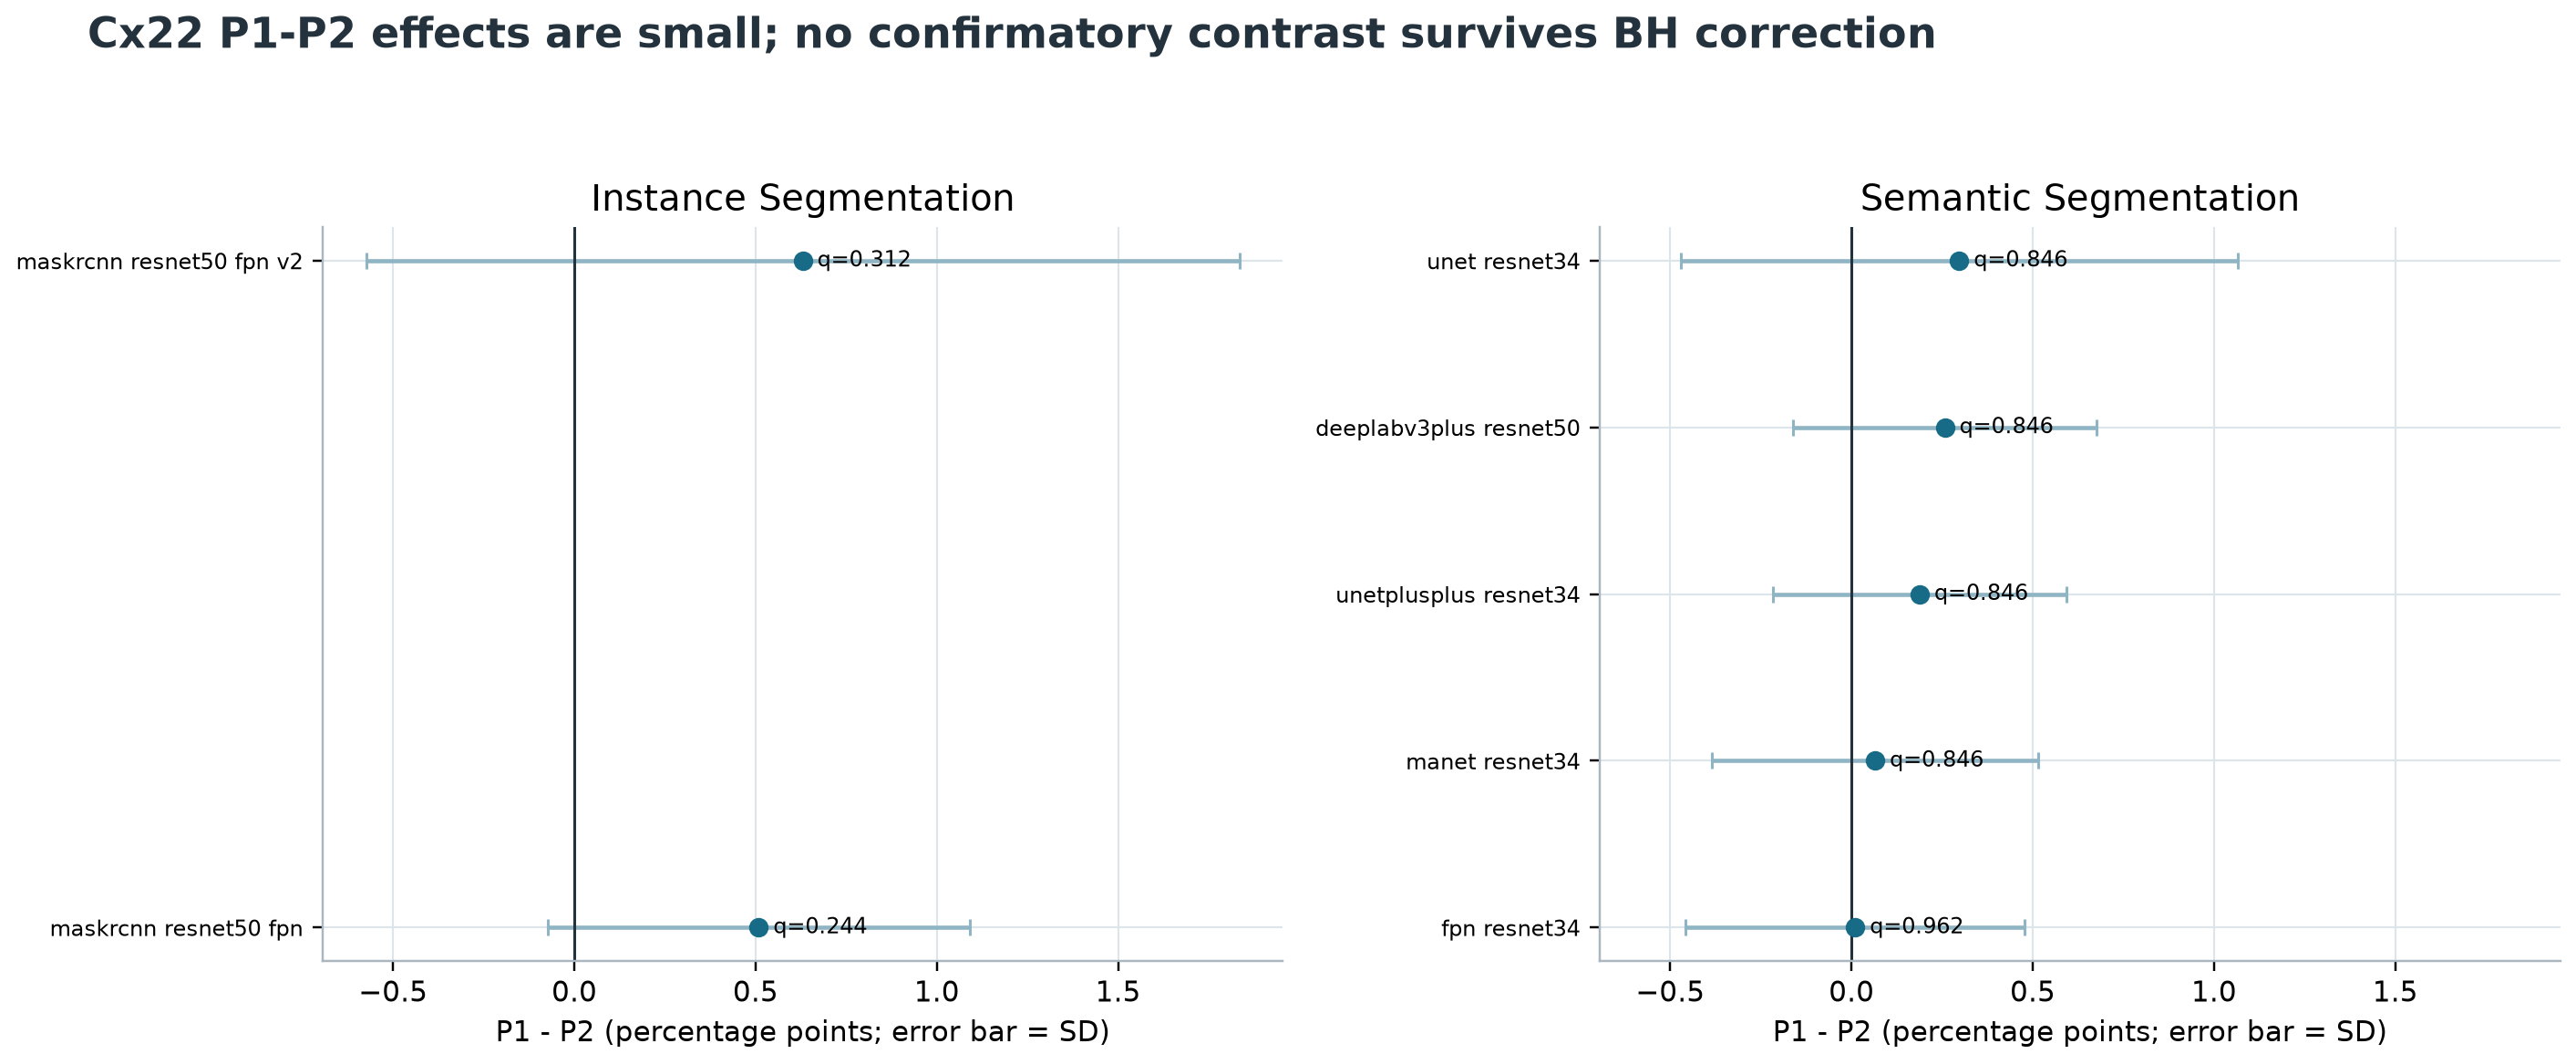
\includegraphics[width=\textwidth]{cx22_contrasts.png}
\caption{Cx22 paired contrast overview. Positive values favor the crop-level protocol. The plot separates point-estimate consistency from multiplicity-adjusted evidence.}
\label{s1:fig:cx22-contrasts}
\end{figure}

No primary Cx22 test survives BH correction. The size-matched \protocol{P1$'$}$-$\protocol{P2} Mask R-CNN contrast has raw $p=0.0377$, $d_z=1.368$, and $q=0.1508$; it is not promoted to a significant claim. In the explicitly secondary \protocol{P2}$-$\protocol{P3} family, FPN has raw $p=0.0226$ and $d_z=1.613$; it remains secondary and is not used to rescue the main conclusion.

Semantic model ranking is comparatively stable: Kendall's $\tau=0.8$ with bootstrap interval [0.6, 1.0], $p=0.0833$, and one of ten model pairs reordered. With only two instance models, $\tau=1.0$ but its bootstrap interval spans [$-1$,1], which is appropriately uninformative.

\section{Training failures, recovery, and runtime}

The first MAnet \protocol{P1}, seed-17 attempts produced non-finite losses at epochs 23 and 24 under FP16, despite dynamic loss scaling. Retaining an epoch-22 model or changing only that seed would have biased the matrix. The matrix stopped at 100 of 175 cells, the failure was amended in writing, and every MAnet cell was restarted in FP32 from its fixed seed. The corrected runs also set \artifact{CUBLAS_WORKSPACE_CONFIG=:4096:8} before any corrected MAnet or instance result existed.

Instance segmentation exposed a different failure: not numerical instability, but pipeline starvation. Per-epoch test inference, CPU pairwise mask matching, and network-filesystem checkpoint writes made GPUs wait. The final endpoint was already preregistered, so evaluation was restricted to the final epoch, exact binary intersections moved to the GPU, checkpoints became five-epoch recovery files, and immutable arrays were staged locally. These changes preserved the endpoint and substantially improved utilization; they did not alter splits, seeds, models, thresholds, or the final metric.

\begin{figure}[H]
\centering
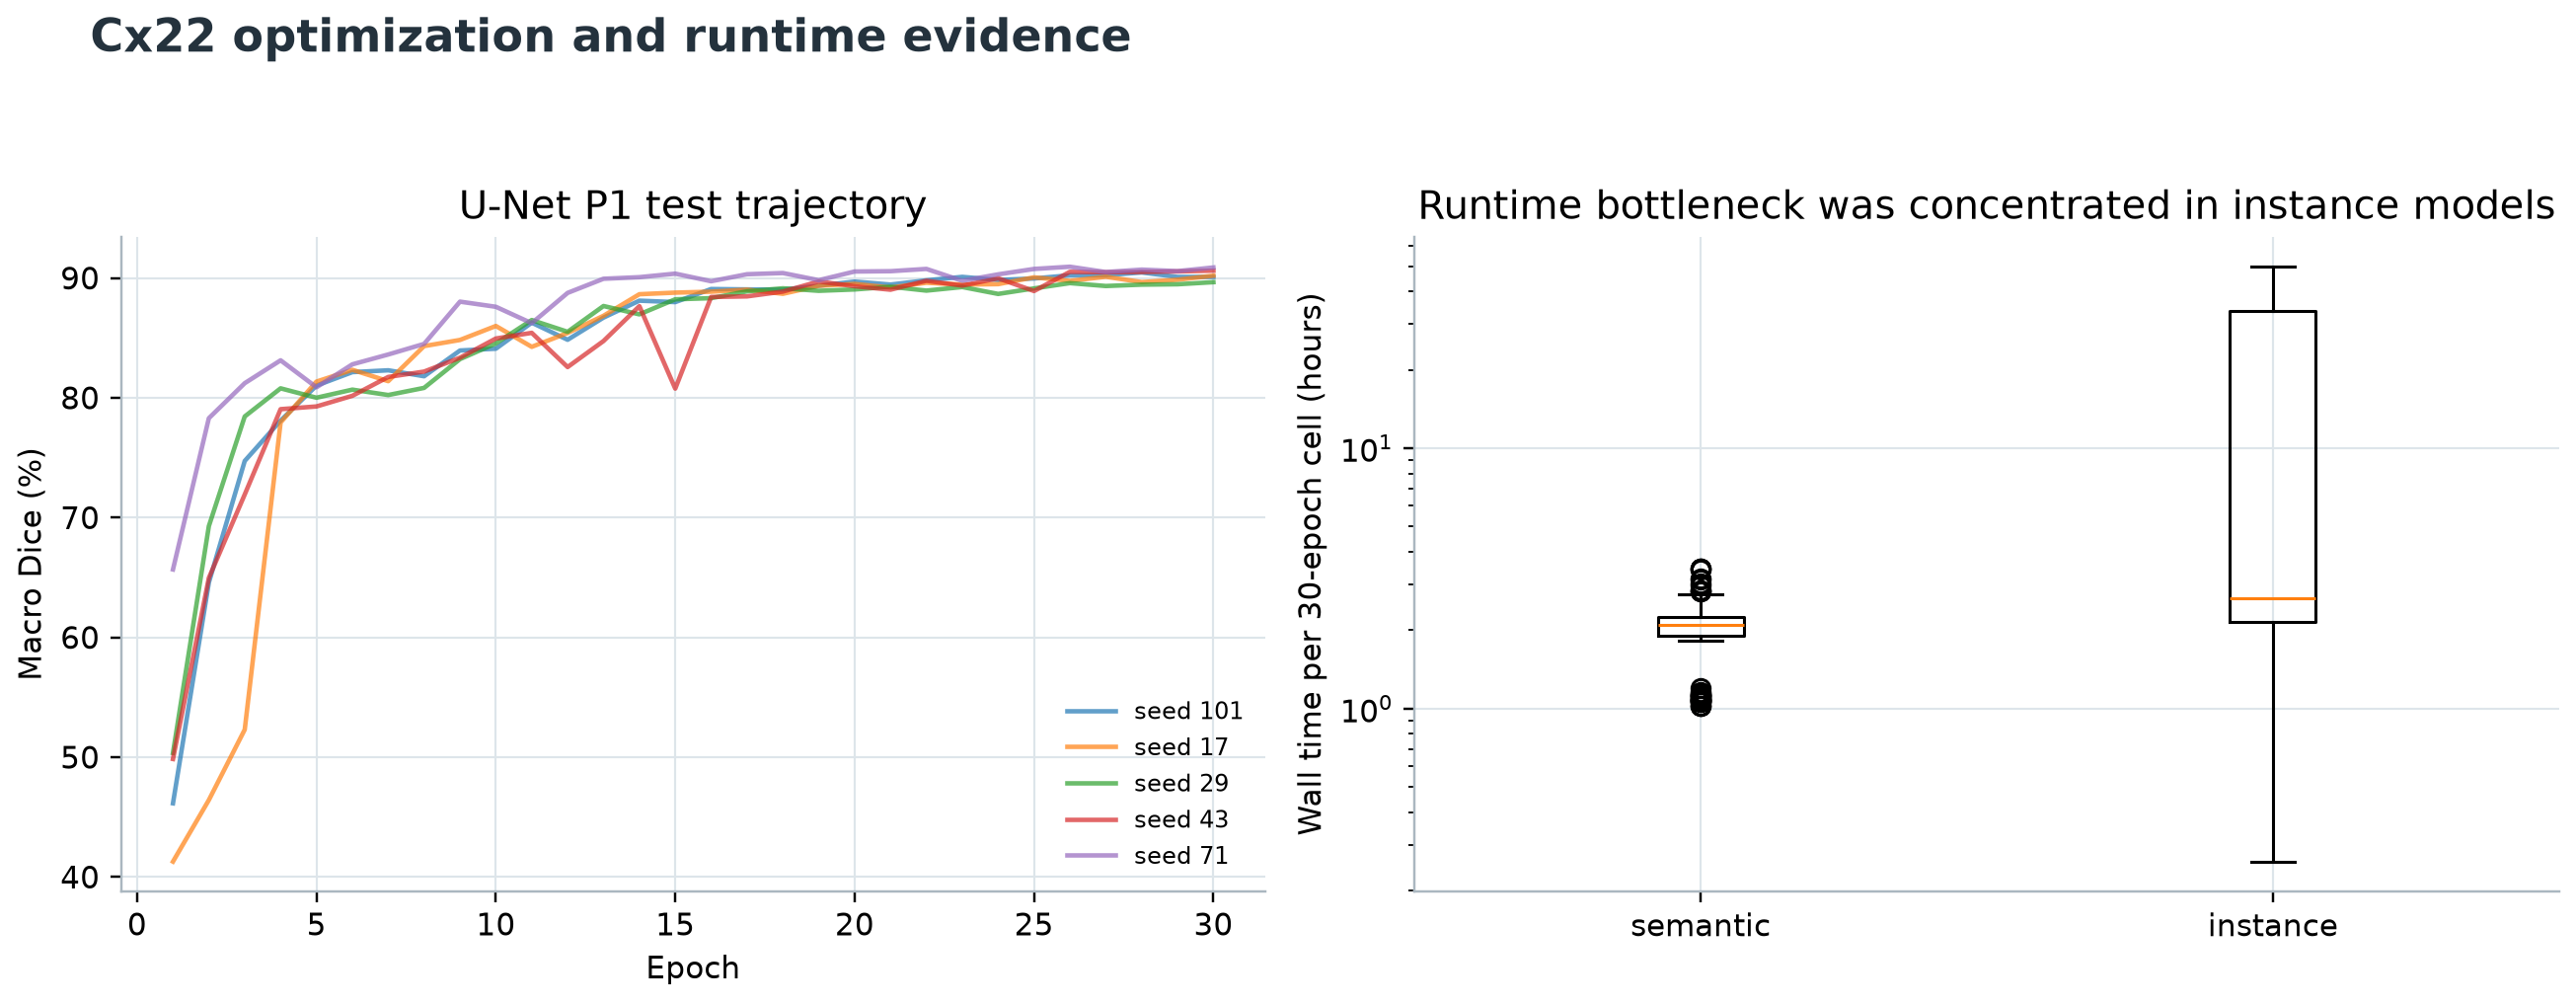
\includegraphics[width=\textwidth]{cx22_training_runtime.png}
\caption{Cx22 run-time distribution. Instance segmentation dominates the computational cost and has a long tail; the plot makes the operational bottleneck explicit.}
\label{s1:fig:cx22-runtime}
\end{figure}

The 125 semantic cells consumed 253.33 summed run-hours, with median cell time 2.09 hours. The 50 instance cells consumed 646.76 summed run-hours, with median 2.64 hours and range 0.258--49.79 hours. The complete Cx22 matrix consumed 900.08 summed run-hours. Up to three jobs were concurrent, so the sum is not wall-clock project duration.

As in classification, final model weights and per-pixel predictions were not retained after the completed JSON was written. Figure~\ref{s1:fig:cx22-labels} therefore visualizes real released ground truth, not a simulated qualitative prediction. A post-hoc prediction gallery would require fresh inference and is deliberately outside the frozen record.

% Carried over verbatim from monograph/main.tex (Study 1 record, 13 Sep 2026).
\chapter{Statistical analysis in full}\label{s1:ch:ch12_statistical_analysis_in_full}

\section{The experimental unit is the seed-paired run}

Every reported neural summary uses the five fixed seeds 17, 29, 43, 71, and 101 and gives the arithmetic mean with sample standard deviation ($n-1$ denominator). The protocol contrast is paired by seed. This pairing removes seed-to-seed variation that affects both arms and prohibits a favorable run in one protocol from being compared with an unrelated run in another.

For values $m_s$ over $S=5$ seeds,
\begin{equation}
\bar m=\frac{1}{S}\sum_{s=1}^{S}m_s,\qquad
s_m=\sqrt{\frac{1}{S-1}\sum_{s=1}^{S}(m_s-\bar m)^2}.
\end{equation}
A summary is suppressed if fewer than five seeds are present. This is enforced in code rather than remembered during table writing.

\section{Test-selection rule}

The preregistered rule first applies Shapiro--Wilk~\cite{shapiro1965normality} to the five paired differences. If $p\geq0.05$, a two-sided paired $t$-test is emitted; otherwise a two-sided Wilcoxon signed-rank test~\cite{wilcoxon1945rank} is emitted. The effect is Cohen's $d_z$ for a $t$-test and rank-biserial correlation for Wilcoxon. All-zero differences are descriptive; a constant nonzero difference has an infinite standardized effect by definition and is flagged explicitly.

With only five observations, normality screening has little power and neither test can create information that is not present. The rule is retained because it was specified before results, but conclusions emphasize effect direction, variability, and corrected evidence rather than treating the test label as a guarantee.

\section{Bootstrap effect intervals}

Ten thousand deterministic bootstrap replicates resample the vector of paired differences with replacement. Each replicate recomputes the relevant effect-size estimator. The interval is the 2.5th and 97.5th percentiles of finite estimates. A SHA-256-derived bootstrap seed from the dataset/model/protocol key makes intervals repeatable without coupling them to the training seed.

These are intervals for the standardized effect, not raw mean-score intervals. Because $n=5$, they can be wide or asymmetric and can contain values much larger than the point estimate. That apparent awkwardness is a correct display of limited information.

\section{Multiplicity families}

Benjamini--Hochberg~\cite{benjamini1995fdr} is applied once to the exact supplied family:
\begin{itemize}
  \item SIPaKMeD classification: all six \protocol{P1}$-$\protocol{P2} and six \protocol{P1$'$}$-$\protocol{P2} tests in the registered joint family;
  \item Cx22 semantic: five \protocol{P1}$-$\protocol{P2} and five \protocol{P1$'$}$-$\protocol{P2} tests;
  \item Cx22 instance: two \protocol{P1}$-$\protocol{P2} and two \protocol{P1$'$}$-$\protocol{P2} tests.
\end{itemize}
Secondary \protocol{P2}$-$\protocol{P3} tests and ranking stability are clearly labeled secondary/unadjusted and cannot substitute for a failed primary family. For ordered raw values $p_{(1)}\leq\cdots\leq p_{(M)}$, BH computes monotone adjusted values based on
\begin{equation}
q_{(i)}=\min_{j\geq i}\left(1,\frac{M}{j}p_{(j)}\right).
\end{equation}

\section{Structural sampling error}

The expected parent-straddle probability for a parent of size $k$ and 80/20 crop assignment is exact: $1-0.8^k-0.2^k$. Dataset-level analytic expectations average this quantity over recovered parents. Monte Carlo means and SDs over the same five fixed seeds check the split implementation, while 10,000 additional simulations form the broad analytic envelope recorded in the structural table. Herlev is a stronger software test than a confidence interval: because every parent has $k=1$, both the analytic and observed straddle fractions must be exactly zero.

\section{Why a non-significant result is not ``no effect''}

A BH-adjusted $q>0.05$ says that the current five-seed family does not meet its declared evidential threshold. It does not prove a zero effect. Conversely, six same-sign classifier means do not license six independent significance claims. The report keeps both facts visible: the direction is consistent, and the adjusted confirmatory evidence is insufficient.

% Carried over verbatim from monograph/main.tex (Study 1 record, 13 Sep 2026).
\chapter{Execution lifecycle, failures, and demotivations}\label{s1:ch:ch13_execution_lifecycle_failures_and_demotiv}

\section{Run inventory}

\begin{table}[H]
\centering
\caption{Frozen neural-run inventory and summed run time.}
\label{s1:tab:inventory}
\begin{tabular}{lrrr}
\toprule
Experiment & Cells & Retained complete & Summed hours \\
\midrule
SIPaKMeD classification & 120 & 120 & 8.48 \\
SIPaKMeD parent probe & 30 & 30 & 5.75 \\
Cx22 semantic segmentation & 125 & 125 & 253.33 \\
Cx22 instance segmentation & 50 & 50 & 646.76 \\
\midrule
Total & 325 & 325 & 914.31 \\
\bottomrule
\end{tabular}
\end{table}

The total is the sum of recorded per-run elapsed seconds. It is intentionally not converted into ``GPU-days'' without qualification: host I/O stalls and overlapping runs mean elapsed seconds include more than active kernel time, while three concurrent GPUs mean the sum exceeds calendar duration.

\section{The first classification matrix was invalid}

An early classifier attempt used scikit-learn 1.7.2. The resulting \protocol{P2} split counts disagreed across cells, violating the requirement that every architecture see the same seed-specific observations. Twelve JSON files from that attempt were excluded in full. The environment was pinned to scikit-learn 1.9.0, the expected split hashes and counts were made acceptance checks, and the entire 120-cell matrix restarted. Three additional one-epoch files were smoke tests and were never mixed into the result family.

This failure changed the engineering standard: a result is not accepted merely because training finished. Dataset name, architecture, protocol, seed, train/test counts, library versions, provenance hash, split hash, Git SHA, GPU field, metric finiteness, and history length must all match the matrix contract.

\section{MAnet numerical failure}

MAnet attention matrix multiplications overflowed under FP16 late in training. Two attempts failed non-finitely at epochs 23 and 24 for the first MAnet cell. The tempting choices---use the last finite epoch, lower the learning rate only for that cell, or replace seed 17---would each change the estimand after seeing its behavior. The accepted response was broader: freeze an amendment, run every MAnet cell in FP32, restart from the same seeds, and keep the failures in the record.

\section{The host bottleneck}

The remote machine had three available RTX A6000 GPUs but a separate storage/host bottleneck. Heavy concurrent decoding and checkpoint writes could make all GPUs appear slow and could destabilize the SSH session. Launchers therefore queried memory usage and utilization, admitted no more than three idle devices, used atomic result writes, and kept resumable checkpoints. The instance-segmentation redesign reduced expensive network I/O and moved exact matching work to the GPU.

\begin{decisionbox}{What did not work}
The project did not produce a universal multiplicity-corrected classifier inflation result, did not validate the preregistered classification ordering, did not retain prediction-level classifier outputs for a confusion matrix, and has not yet demonstrated a raw-download-to-Table-1 run on a machine that has never seen the project. Each limitation is part of the result, not a cosmetic omission.
\end{decisionbox}

\section{Research stop and evidence freeze}

After the publication verdict, exploration stopped. No architecture was added to chase significance; no seed was replaced; no endpoint was changed; no new confusion matrix was generated. The long-form report reconstructs plots only from frozen aggregates and epoch histories. Images used to explain Otsu/Telea and Cx22 label decoding are implementation demonstrations from locally available released data and are labeled as such.

% Carried over verbatim from monograph/main.tex (Study 1 record, 13 Sep 2026).
\chapter{Verification against the acceptance contract}\label{s1:ch:ch14_verification_against_the_acceptance_cont}

\section{Gate-by-gate status}

\begin{figure}[H]
\centering
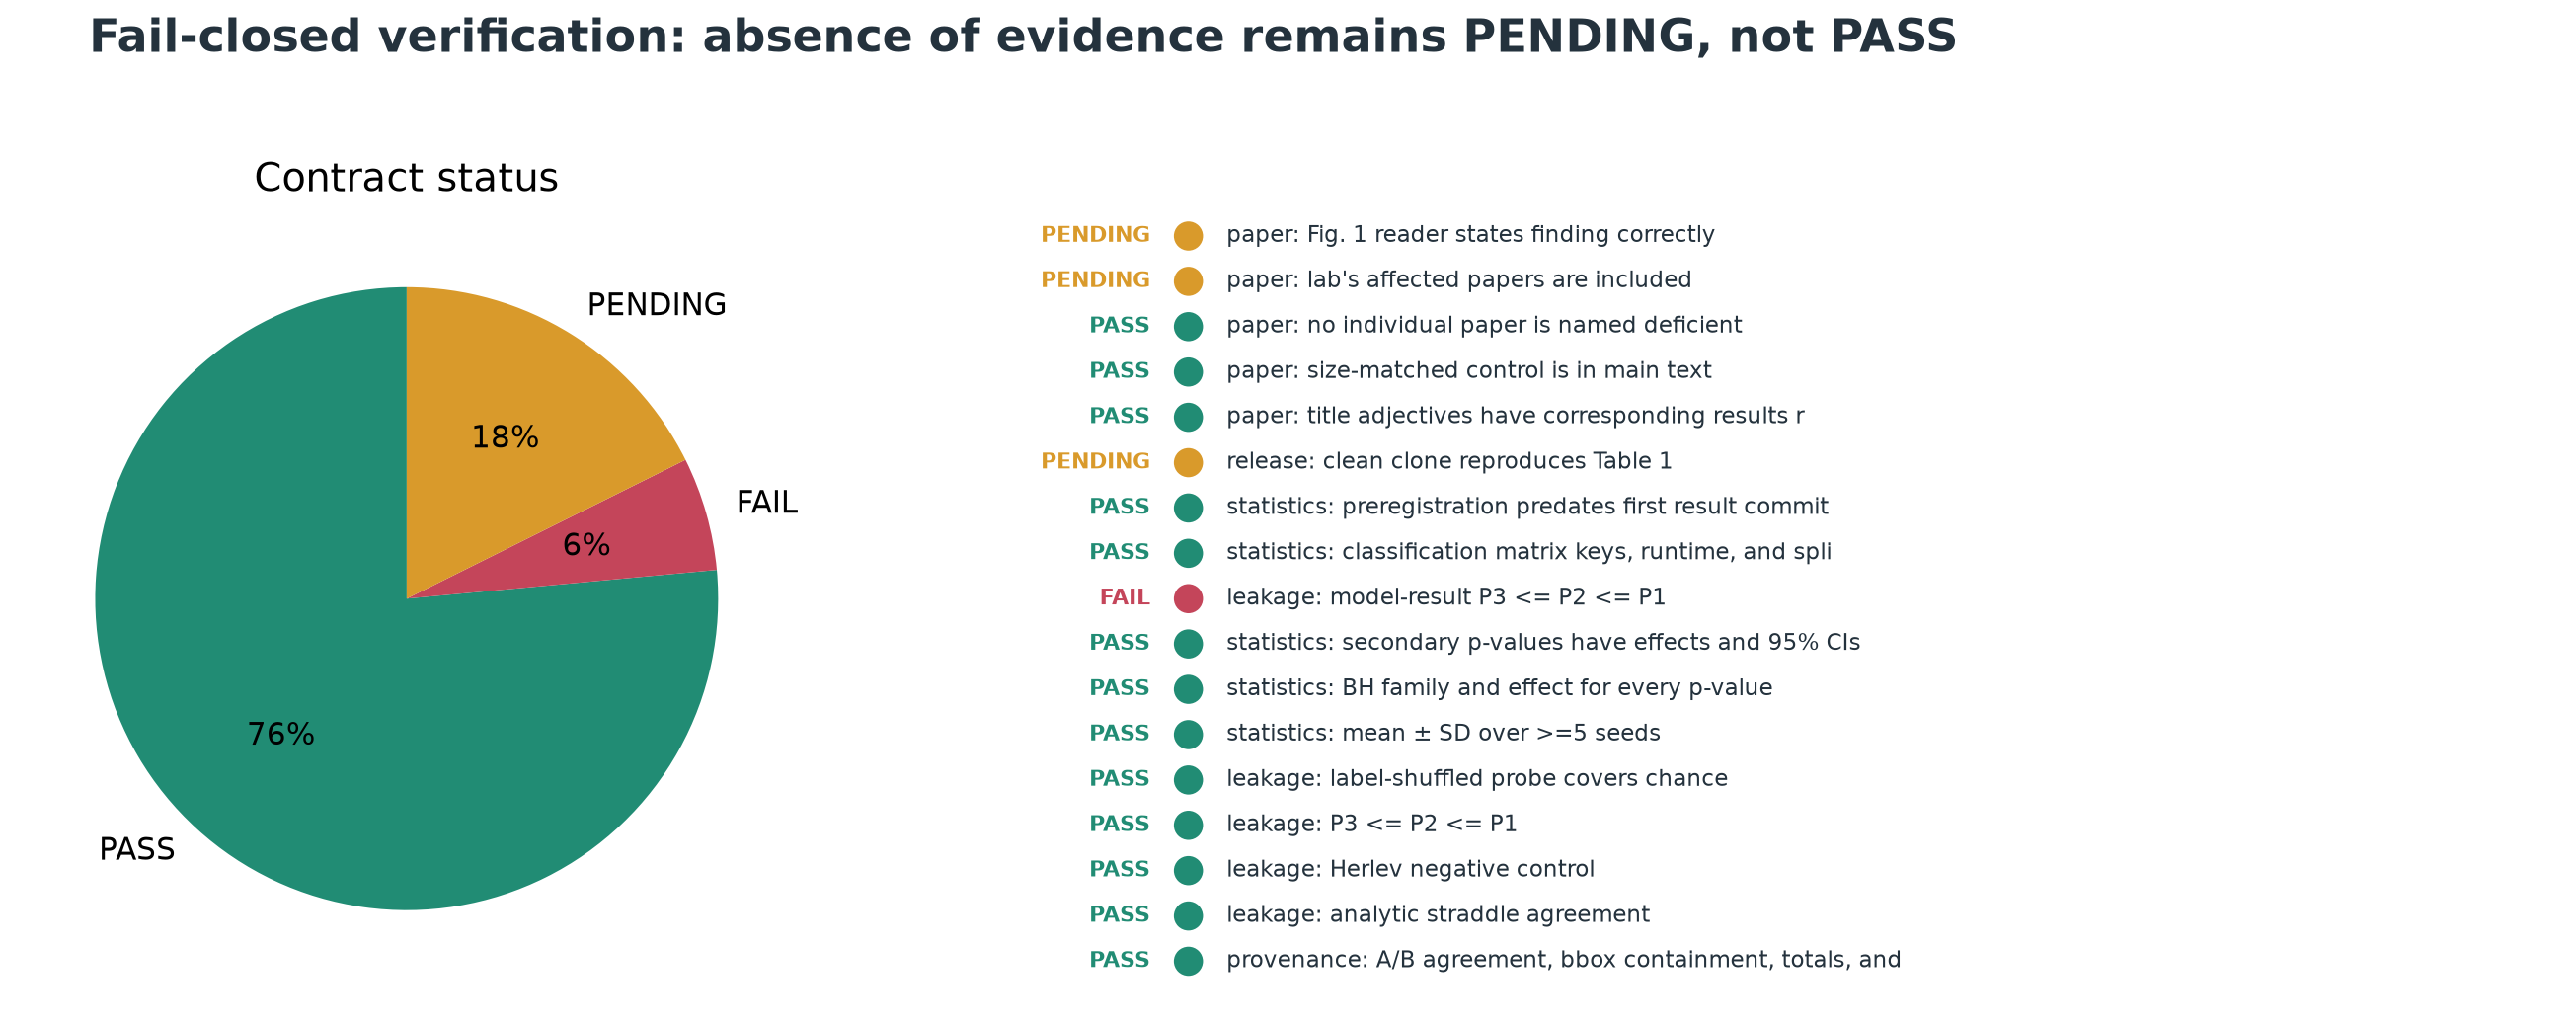
\includegraphics[width=\textwidth]{acceptance_dashboard.png}
\caption{Machine-readable acceptance status: 13 gates pass, one fails, and three remain pending. A pending release gate is not painted green simply because the numerical experiments are complete.}
\label{s1:fig:acceptance}
\end{figure}

\begin{longtable}{p{0.29\textwidth}p{0.14\textwidth}p{0.45\textwidth}}
\caption{Acceptance contract with evidence.}
\label{s1:tab:acceptance}\\
\toprule
Gate & Status & Evidence \\
\midrule
\endfirsthead
\toprule
Gate & Status & Evidence \\
\midrule
\endhead
\bottomrule
\endfoot
SIPaKMeD branch agreement $\geq99\%$ & \pass & 4,049/4,049 mappings agree (100\%). \\
Every bbox lies in parent bounds & \pass & 4,049/4,049 pass geometry checks. \\
Crop and per-class parent totals match & \pass & 4,049 crops; parent vector 126/108/238/271/223. \\
Observed straddle matches analytic prediction & \pass & All audited multi-crop datasets fall inside the recorded simulation envelope. \\
Herlev has no structural effect & \pass & All five seeds return exactly zero in \protocol{P1}; \protocol{P2}/\protocol{P3} also zero. \\
\protocol{P3}$\leq$\protocol{P2}$\leq$\protocol{P1}, structural & \pass & Grouped protocols eliminate measured parent sharing. \\
Shuffled probe confirms chance & \pass & 95\% $t$ interval [$-0.1385$, 0.4687]\% contains 0.2358\%. \\
Every neural summary has $\geq5$ seeds & \pass & 120 classifier, 30 probe, and 175 Cx22 files pass matrix completeness. \\
Plan predates first result commit & \pass & 22 Aug 2026 04:54:10 IST versus 13:22:42 IST. \\
BH applied over stated families & \pass & Stored family labels and $q$ values are reproduced from the exact supplied rows. \\
Effect accompanies every inferential $p$ & \pass & $d_z$, rank-biserial, or Kendall $\tau$ is present. \\
Classifier \protocol{P3}$\leq$\protocol{P2}$\leq$\protocol{P1} & \fail & Only ResNet-50 and ViT-B/16 pass; four of six fail. \\
Cx22 model ordering & \pass & All five semantic and two instance rows pass. \\
Official Cx22 parent disjointness & \pass & Multi-Train and Multi-Test have no shared recovered source parent. \\
Virgin-host clean-clone reproduction & \pending & Script exists, but execution evidence from a never-used host is absent. \\
Lab's own affected papers in audit & \pending & No verified crosswalk in the frozen repository. \\
Figure-1-only independent reader & \pending & No documented colleague response in the frozen repository. \\
\end{longtable}

\section{Why the classification ordering gate fails}

The structural ordering and model-score ordering are different propositions. \protocol{P3} has stricter grouping than \protocol{P2}, but it also creates a different balanced partition. Removing a small duplicate-connected component can alter class composition, parent difficulty, and which observations land in test. A finite test set can therefore score higher under the stricter split even though it contains less structural sharing. The failure warns against using monotonic score ordering as a definition of correctness; leakage absence should be checked directly from IDs and components.

\section{Release-readiness boundary}

The repository contains a one-script verification path, but the strongest release criterion requires a truly clean machine that has never held the repository or data. Running the script on the development host, even in a new directory, would not fully establish that environmental condition. This report therefore leaves the release gate pending. The same standard applies to the human communication gate and lab-paper crosswalk: absence of evidence is not converted into a pass.

% Carried over verbatim from monograph/main.tex (Study 1 record, 13 Sep 2026).
\chapter{Interpretation, limitations, and practical guidance}\label{s1:ch:ch15_interpretation_limitations_and_practical}

\section{What the evidence supports}

The source hierarchy is real and recoverable. Random crop splitting predictably separates siblings. In SIPaKMeD it can also put overlapping source pixels into training and test. Parent identity is learnable even after large parts of the apparent cell signal are removed. Parent- and component-disjoint protocols eliminate the directly measured sharing. These conclusions follow from deterministic identities, geometry, and controls, not from a single favorable neural score.

The downstream effect is subtler. Every tested \protocol{P1}$-$\protocol{P2} mean is positive, including six classifiers and seven segmentation models, but the Cx22 semantic differences are often tiny and none of the task-specific confirmatory families survives BH correction. The evidence supports changing split construction because independence is a design requirement, not because a guaranteed score penalty has been estimated.

\section{Two hard visual structures in Cx22}

The most persistent semantic error source is the nucleus channel. Nuclei occupy fewer pixels, so boundary uncertainty has a larger Dice penalty; pale nuclei and overlaps further reduce contrast. The second hard structure is touching cytoplasm instances. A union mask can remain visually plausible while an instance model merges two touching cells; maximum matching then assigns a good overlap to one target and zero or low overlap to the other. These explanations correspond to the actual label geometry in Figure~\ref{s1:fig:cx22-labels} and the channel results in Figure~\ref{s1:fig:cx22-channels}.

\section{Real limitations}

\begin{enumerate}[leftmargin=2em]
  \item \textbf{Dataset hierarchy stops at the released identifier.} SIPaKMeD fields and Cx22/CRIC sources are not guaranteed to be patient IDs. Parent-disjoint is therefore necessary but may not be sufficient for clinical independence.
  \item \textbf{Five seeds leave broad uncertainty.} The complete matrix is large in GPU hours but small in inferential replication. Shapiro screening and bootstrap effects are fragile at $n=5$.
  \item \textbf{No clinical validation.} The study audits public research benchmarks; it does not estimate screening sensitivity, specificity, prevalence calibration, reader impact, or deployment safety.
  \item \textbf{Hardware and host constraint.} Execution occurred on one login node with at most three A6000 GPUs and an unstable I/O bottleneck. Wall times are not portable performance claims.
  \item \textbf{Probe transformations are not surgical interventions.} Grayscale, normalization, inpainting, and high-pass filtering each alter multiple cues. They localize signal classes but do not identify a unique causal artifact.
  \item \textbf{Near-duplicate grouping is conservative and calibrated synthetically.} It found no exact cross-parent duplicates and validated candidate detection on 3 positive/100 negative synthetic examples, but it is not a proof that every biological near-duplicate was linked.
  \item \textbf{Prediction-level artifacts were not retained.} Post-hoc classifier confusion matrices and qualitative prediction panels cannot be reconstructed without new inference.
  \item \textbf{Reproduction remains pending on a virgin host.} Dependency or URL drift may still be exposed by that final test.
\end{enumerate}

\section{Recommended evaluation rule}

For any crop-derived cytology dataset, publish at least four fields for every released observation: a stable observation ID, an acquisition/source parent ID, a patient/specimen ID when ethically and legally possible, and a duplicate-component ID if cross-parent duplication was audited. Construct folds at the highest available independent level and publish the exact fold manifest. Report sample counts at both observation and parent levels. Never compare methods under nominally identical dataset names unless the split identifiers also match.

\section{What to say in a paper}

The defensible headline is: ``Random crop-level evaluation in public cervical cytology can place sibling and even pixel-overlapping crops across train and test; source-disjoint manifests remove this non-independence.'' A stronger sentence---``all published scores are inflated''---is not supported. No individual prior paper needs to be named as deficient; the target is a reusable benchmark practice.

% Carried over verbatim from monograph/main.tex (Study 1 record, 13 Sep 2026).
\chapter{Reproduction and release engineering}\label{s1:ch:ch16_reproduction_and_release_engineering}

\section{From owner downloads to structural Table 1}

\begin{figure}[H]
\centering
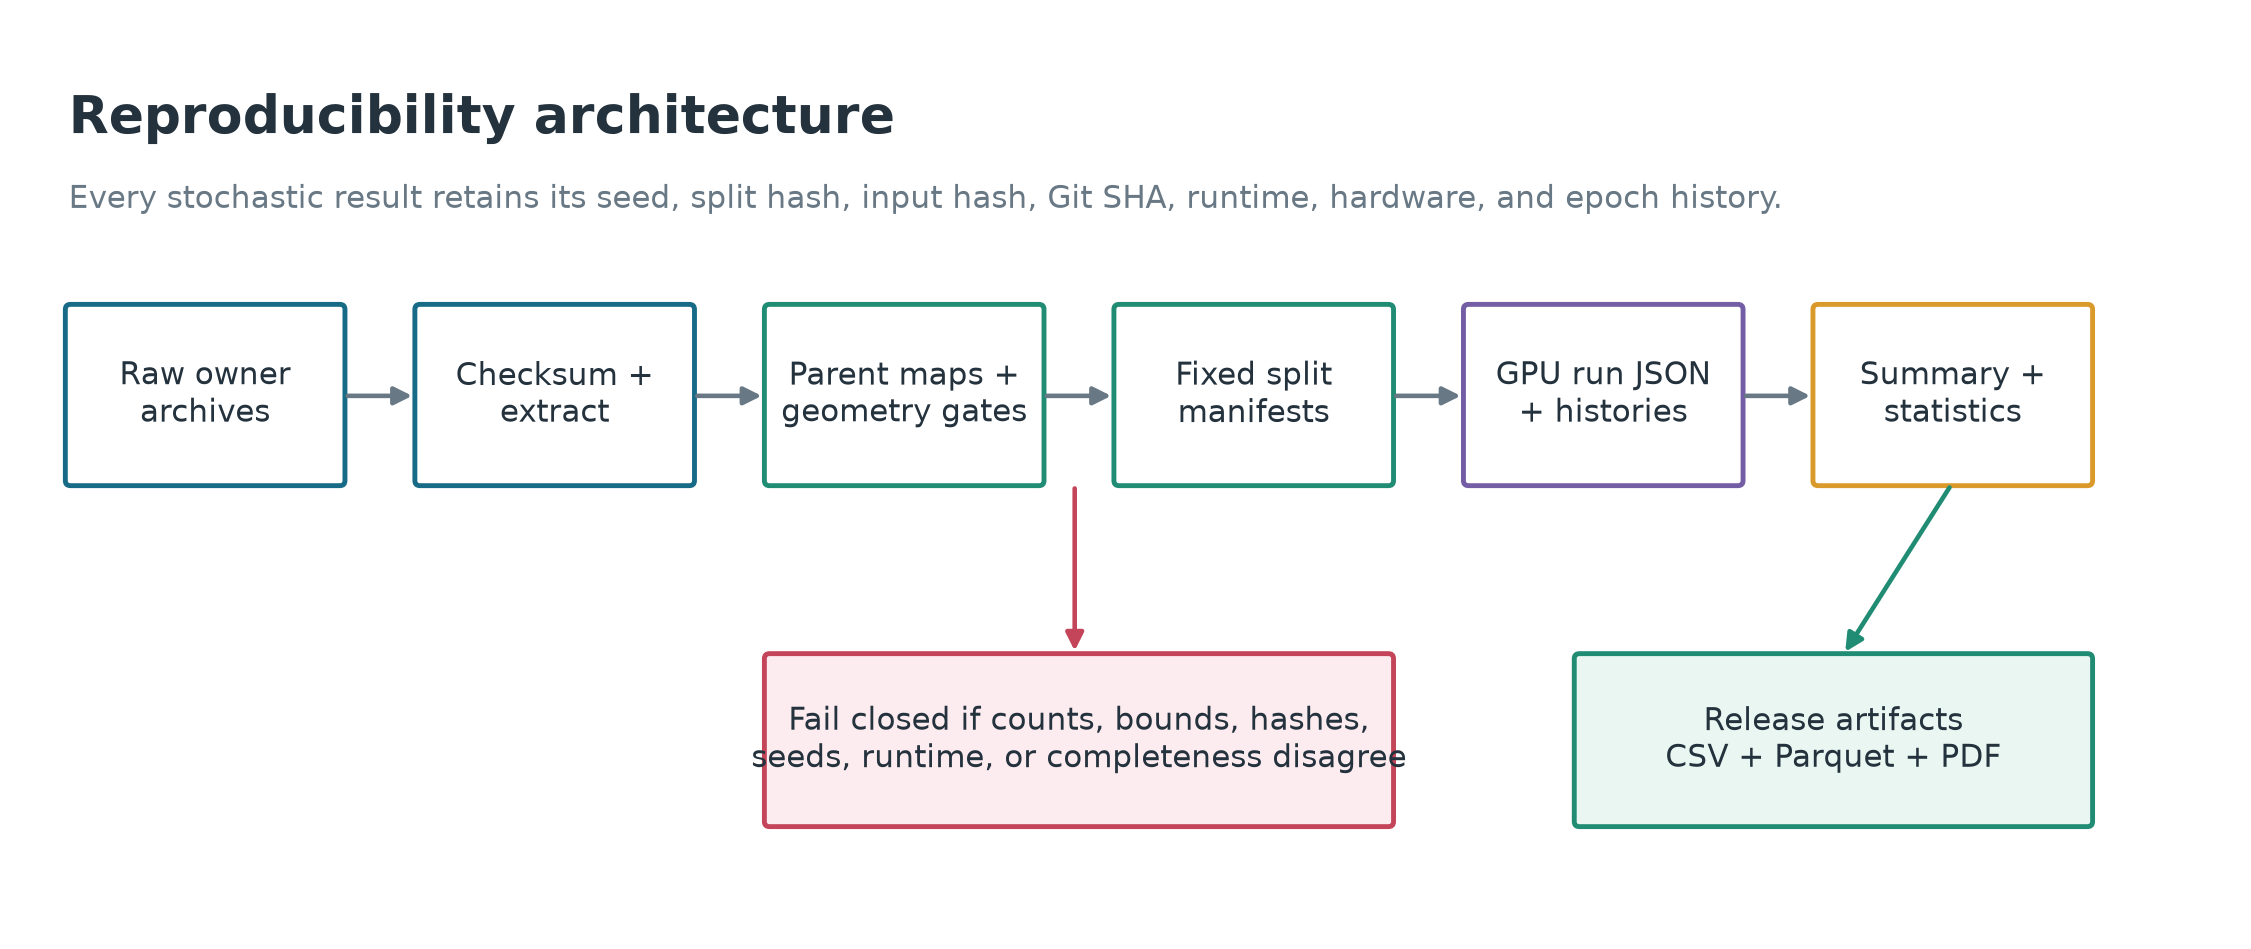
\includegraphics[width=\textwidth]{reproducibility_pipeline.png}
\caption{The intended clean-clone path. Each boundary writes an auditable artifact and performs validation before the next stage begins.}
\label{s1:fig:reproduction}
\end{figure}

The GPU-free structural result has one public entry point:
\begin{lstlisting}[style=cyto,language=bash,caption={Raw-download-to-Table-1 entry point.}]
./scripts/reproduce_table1.sh
\end{lstlisting}
The script performs a locked dependency sync; downloads all declared owner files with at most three connections; verifies exact sizes and SHA-256 values; extracts archives; recovers SIPaKMeD, Cx22, CRIC, and Herlev provenance; runs the SIPaKMeD duplicate and pixel-overlap audits; creates fixed splits; and emits the dataset-level and seed-level structural tables.

Raw images are intentionally excluded from version control. The repository distributes URLs, checksums, IDs, coordinates, derived maps, split assignments, and results, subject to each source's terms. In particular, Cx22/CCEDD assets are non-commercial research resources and are not repackaged in this report.

\section{Clean-clone attestation}

The wrapper requires a repository URL and a destination that does not yet exist:
\begin{lstlisting}[style=cyto,language=bash,caption={Clean-clone verification wrapper.}]
./scripts/verify_clean_clone.sh \
  REPOSITORY_URL NEW_DESTINATION [GIT_REF]
\end{lstlisting}
It uses \artifact{git clone --no-local}, optionally checks out an exact detached ref, runs the reproduction script, and writes an attestation. A human/operator must set \artifact{CYTOFAIR_VIRGIN_HOST_ATTESTED=YES} only on a host that genuinely has never seen the project. The current repository lacks that final attested evidence, so release remains pending rather than assumed.

\section{Pinned software and result metadata}

The package requires Python 3.11 or newer. The result contract records NumPy 2.5.2, pandas 3.0.5, SciPy 1.18.1, scikit-learn 1.9.0, Pillow 12.3.0, OpenCV 5.0.0, PyTorch 2.9.0+cu128, torchvision 0.24.0+cu128, and CUDA 12.8 for the accepted classifier matrix. The lock file, not these prose values, is the install authority. The explicit versions remain useful diagnostics when a future lock update changes a hash.

\section{Atomicity and resumability}

Long GPU runs write checkpoints locally and copy them to a temporary destination name before atomic rename. A checkpoint is accepted only when its protocol, architecture, seed, and manifest hash match the requested cell. The launcher skips a result only after validating its completed JSON. A second launch can therefore resume interrupted work without accepting a mismatched or half-written file.

\section{Human-readable and machine-readable layers}

The project separates three layers:
\begin{itemize}
  \item \textbf{canonical data}: Parquet provenance maps and CSV split assignments;
  \item \textbf{machine evidence}: JSON run records, CSV summaries, hashes, and acceptance states;
  \item \textbf{human interpretation}: Markdown reports, figures, the conference paper, and this lifecycle monograph.
\end{itemize}
This prevents a narrative edit from changing the measured evidence and makes it possible to regenerate prose tables from structured files.

% Carried over verbatim from monograph/main.tex (Study 1 record, 13 Sep 2026).
\chapter{Reusable outputs and future work}\label{s1:ch:ch17_reusable_outputs_and_future_work}

\section{What exists now}

The most durable asset is not a new image collection. It is a stable interface between released observations and independent units: canonical parent maps, duplicate-component identifiers, fixed split CSVs, adjacent hashes, a leak-checking API, a run JSON schema, and paired statistics. A downstream model joins on \artifact{crop_id}; it never infers a split from row order or regenerates folds with a library default.

\section{Two publication units}

The conference unit is the complete provenance/leakage argument, mechanism probe, fixed split release, and matched SIPaKMeD rescore. A journal extension can add a separately preregistered annotation study, expanded cross-dataset validation, a broader detector ensemble, and power-oriented learning curves. These are partitioned future studies, not unreported parts of the present evidence.

\section{Projects unblocked}

\begin{table}[H]
\centering
\caption{Immediate technical reuse. These rows describe enabled work, not completed future experiments.}
\label{s1:tab:reuse}
\begin{tabularx}{\textwidth}{lXX}
\toprule
Project & Reused asset & Work no longer rebuilt \\
\midrule
F3: Cx22 seed robustness & Parent map, fixed seeds, run schema, mean/SD and paired inference & Source grouping, seed ledger, rescore scaffold \\
F8: cross-dataset transfer & Canonical maps, split API, runtime metadata, label-crosswalk slot & Leakage-safe source folds and experiment provenance \\
F2: foundation encoders & P1/P1$'$/P2/P3 files and architecture-neutral summarizer & Fair split comparison, seed accounting, BH/effect reporting \\
\bottomrule
\end{tabularx}
\end{table}

\section{Pre-specified V2 in fish imagery}

Fish-Pak contains three views of the same specimen; Croatian Fish contains frames sampled at one frame per second from continuous BRUV/DOV video. The independent units become specimen and video episode. The planned V2 will: recover those units, compute analytic and observed frame straddling, construct specimen/episode-disjoint manifests, run the identity probe, and re-score fixed baselines under \protocol{P1}/\protocol{P1$'$}/\protocol{P2}/\protocol{P3}. No fish-domain result is claimed here.

\section{Adoption goal}

If versioned CytoFair manifests become the default evaluation interface, future papers can cite both the original dataset and the split asset while reporting exactly which parent-disjoint partition they used. This is an intended impact pathway, not a citation prediction or an empirical result.

% Carried over verbatim from monograph/main.tex (Study 1 record, 13 Sep 2026).
\chapter{Conclusion}\label{s1:ch:ch18_conclusion}

This project asked whether a file-level train/test boundary corresponds to an independent acquisition boundary in public cervical cytology. It recovered and validated the hidden observation-to-parent hierarchy across four datasets, quantified the analytic and observed structural sharing, demonstrated literal source-pixel sharing in SIPaKMeD, and showed with a shuffled-label-controlled 424-way probe that parent identity remains strongly learnable after multiple cue-removal transformations. It then re-ran six classifiers and seven segmentation models over five fixed seeds and four matched protocols, preserving effect sizes, bootstrap intervals, multiplicity families, failures, and runtime metadata.

The strongest result is methodological: parent-disjoint evaluation is necessary whenever multiple released observations descend from one acquisition unit. The downstream neural results point in a consistent direction but do not justify a universal multiplicity-corrected accuracy-inflation claim. Four of six classifier architectures also violate the preregistered monotonic score ordering, a useful negative result showing that stricter grouping and lower finite-sample score are not synonymous.

CytoFair turns that lesson into reusable artifacts: provenance maps, duplicate components, fixed splits, hashes, fail-closed validators, run ledgers, and a raw-download structural pipeline. The next scientific step is a separately preregistered specimen/episode-disjoint fish-imagery V2; the next release step is a virgin-host clean-clone attestation. Until the latter, the numerical study is complete but the strongest release gate remains honestly pending.


\part{From Study 1 to Study 2: Roadmap and Design}

\chapter{The roadmap and what we did with it}
\label{r:ch:roadmap}

\section{What Study 1 left unresolved}

Study~1 (Part~II) ended with a strong benchmark-construction conclusion and a deliberately weak model-performance
conclusion. Five problems stood between them.

\begin{enumerate}[leftmargin=1.8em]
\item \textbf{One question, six tests.} ``Does crop-level splitting inflate accuracy?'' was tested once per
architecture inside a twelve-test Benjamini--Hochberg family. Every point estimate was positive, every test was
underpowered, and none survived.
\item \textbf{Availability is not use.} A 424-way probe recognised fields far above chance, but that shows the shortcut
is \emph{available}, not that classifiers route their predictions through it.
\item \textbf{Leakage confounded with diversity.} At equal crop counts a crop-level training set contains about 914
distinct fields and a field-level one about 773; P1 differs from P2 in training diversity as well as in leakage.
\item \textbf{One rescored benchmark.} Only SIPaKMeD was rescored for classification; CRIC, whose crop-level split puts a
training parent behind essentially every test cell, was not.
\item \textbf{The host.} The original classification matrix had to be repeated (Chapter~\ref{s1:ch:ch13_execution_lifecycle_failures_and_demotiv}
is the record), and runs were slower than expected for reasons only diagnosed in Study~2 (Section~\ref{r:ch:host}).
\end{enumerate}

\section{The roadmap, item by item}

The October review turned these into a phased roadmap. Table~\ref{r:tab:roadmap} records what was done with every
item, including the ones deliberately not done.

{\small
\begin{longtable}{p{0.24\textwidth}p{0.45\textwidth}p{0.22\textwidth}}
\caption{The scaling roadmap and the response to each item.}\label{r:tab:roadmap}\\
\toprule
Roadmap item & What was done & Status \\
\midrule
\endfirsthead
\toprule
Roadmap item & What was done & Status \\
\midrule
\endhead
\bottomrule
\endfoot
\multicolumn{3}{l}{\textbf{Phase 0: arXiv readiness}} \\
Fresh-clone check & Public repository cloned into a clean directory; its 45 tests pass. The public \texttt{main} branch stops at 22 August and lacks the Cx22 commits and a LICENSE file. & done; push and licence are authors' decisions \\
Text extraction of PDFs & Ligatures broke copy-paste in the drafts; \texttt{glyphtounicode} and T1 encoding added to every preamble. & done \\
Draft claims & The ISBI draft's sentence implying P3 is strictly more conservative than P2 flagged as an overreach; the draft's conclusion now says replication is in progress. & done \\
\multicolumn{3}{l}{\textbf{Phase 1: fix the statistics}} \\
Single omnibus test & One crossed mixed model, \texttt{acc \textasciitilde{} x + (1+x|architecture) + (1|seed) + (1|split)}, with the split random effect that the roadmap's formula omitted (twelve architectures share each test set). & done (H1) \\
Simulation-based power & Custom R simulation of the exact model, 1,000 simulations per design cell, from the Study~1 variance components (Chapter~\ref{r:ch:power}). & done \\
More architectures & Twelve: the six Study~1 models plus ConvNeXt-T, Swin-T, RegNetY-1.6GF, EfficientNetV2-S, MaxViT-T, and self-supervised DINOv2 ViT-S/14. & done \\
15--25 seeds & Twenty, chosen by a registered power rule. & done \\
Preregistration & \texttt{PREREGISTRATION\_STUDY2.md}, registered as Amendment~6 before any Study~2 model was trained. & done \\
Keep predictions, logits, checkpoints & Every run keeps per-crop logits, float16 final weights, and probe-split features; this is what made Amendment~8's evaluation-only arms possible. & done \\
\multicolumn{3}{l}{\textbf{Phase 2: causal arms}} \\
2C leakage vs diversity & Factorial over one common test set at matched crop and field counts. & done (H3) \\
2A fingerprint suppression & Class-conditional parent adversary behind gradient reversal, seven-level $\lambda$ sweep. & done (H5) \\
2B background transplant & Counterfactual composites with a same-parent (sibling) control. & done (H4) \\
\multicolumn{3}{l}{\textbf{Phase 3: generalisation}} \\
Other domains (fish imagery) & Gated on Phase~1 and~2 outcomes; not started. & deferred by design \\
\multicolumn{3}{l}{\textbf{Part 5: datasets}} \\
CRIC second rescore & Rescored with six architectures and ten seeds. & done (H2) \\
Keep Cx22 un-rescored & Kept; the official Cx22 split is parent-disjoint. & done \\
Cx22 literature check & Four open-access studies examined (Section~\ref{r:sec:cx22-lit}). & done \\
JUCYT ground truth & Not publicly available. & not possible \\
\multicolumn{3}{l}{\textbf{Part 6 and Part 8}} \\
Single-column neutral draft & \artifact{paper/v2}, every number generated. & done \\
Avoid scope creep & Study~2 ran only registered arms; Amendment~8 was added after Study~2's results with an explicit justification and its own Holm family. & done \\
\end{longtable}
}

\section{Phase 0 in detail}

The repository was cloned from its public remote into an empty directory, its environment created from the lock file,
and its test suite run: 45 tests passed. Three gaps were recorded in \artifact{reports/study2/phase0_arxiv_checklist.md}.
The public branch stops at 22 August 2026 and does not contain the Cx22 segmentation commits; there is no LICENSE file,
so nobody may legally reuse the toolkit; and several drafts produced PDFs whose ligatures (fi, fl) did not survive
copy-paste. The third was fixed in every preamble. The first two are decisions for the authors and remain open.

\section{The Cx22 literature check}
\label{r:sec:cx22-lit}

The Cx22 release ships an official parent-disjoint split (Multi-Train/Multi-Test). The question was whether downstream
users keep it. Of four open-access studies that train on Cx22, three use the official split. One describes image-level
five-fold cross-validation over all 1,320 generated regions, which pools regions from the same CCEDD source image across
folds. Following the project's no-naming rule for third-party work, only the aggregate is reported
(\artifact{reports/study2/cx22_literature_check.md}).

\section{Post hoc reanalysis of Study 1}

While validating the analysis code, the registered H1 model was fitted to the sixty Study~1 SIPaKMeD P1 and P2 runs. It
gives \RecPostSipEst~pp (SE \RecPostSipSE, Satterthwaite $df=\RecPostSipDf$, $p=\RecPostSipP$). The same model on the
Cx22 semantic-segmentation runs gives \RecPostCxEst\ Dice points ($p=\RecPostCxP$). Both analyses were specified after
the Study~1 data were seen; they motivated Study~2 and supplied its pilot variances, and they are not evidence for
Study~2 (\artifact{results/study2/posthoc/README.md}).

\chapter{The Study 2 preregistration}
\label{r:ch:prereg}

\begin{figure}[H]
\centering
\begin{adjustbox}{max width=\textwidth}
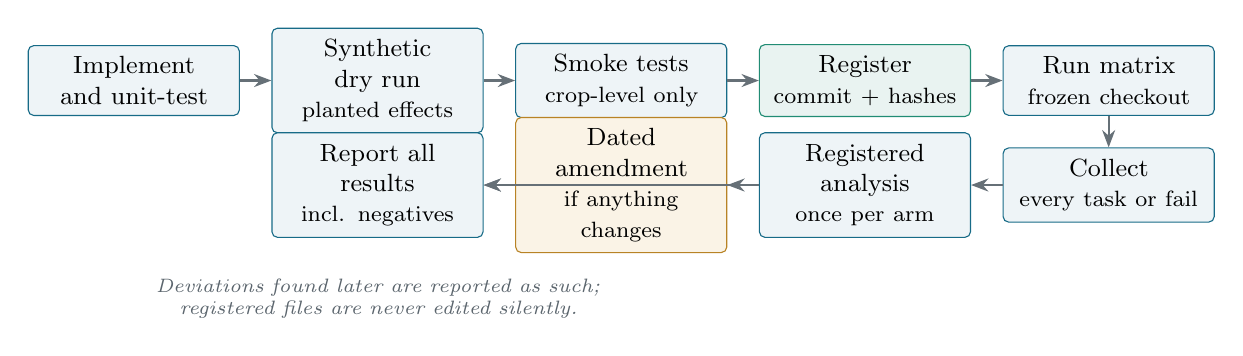
\begin{tikzpicture}[node distance=4mm and 4mm]
\node[box=24mm] (code) {Implement and unit-test};
\node[box=24mm, right=of code] (dry) {Synthetic dry run\\\footnotesize planted effects};
\node[box=24mm, right=of dry] (smoke) {Smoke tests\\\footnotesize crop-level only};
\node[done=24mm, right=of smoke] (reg) {Register\\\footnotesize commit + hashes};
\node[box=24mm, right=of reg] (run) {Run matrix\\\footnotesize frozen checkout};
\node[box=24mm, below=of run] (collect) {Collect\\\footnotesize every task or fail};
\node[box=24mm, left=of collect] (analyse) {Registered analysis\\\footnotesize once per arm};
\node[gold=24mm, left=of analyse] (amend) {Dated amendment\\\footnotesize if anything changes};
\node[box=24mm, left=of amend] (report) {Report all results\\\footnotesize incl. negatives};
\node[note, below=of report, text width=60mm] {Deviations found later are reported as such;\\ registered files are never edited silently.};
\draw[flow] (code) -- (dry); \draw[flow] (dry) -- (smoke); \draw[flow] (smoke) -- (reg);
\draw[flow] (reg) -- (run); \draw[flow] (run) -- (collect); \draw[flow] (collect) -- (analyse);
\draw[flow] (analyse) -- (report); \draw[flow, dashed] (analyse) -- (amend); \draw[flow, dashed] (amend) -- (report);
\end{tikzpicture}
\end{adjustbox}
\caption{The governance loop used for Study 2 (Amendment 6), Amendment 7, Amendment 8, and Amendment 9. The
registration commit fixes the analysis code, split manifests, task files, and cache hashes before any model whose
result it governs is trained.}
\label{r:fig:governance}
\end{figure}


\section{Status at registration}

\texttt{PREREGISTRATION\_STUDY2.md} was committed at \texttt{\RegistrationCommit} (\RegistrationTime) as Amendment~6
of the original plan. At that moment no Study~2 model had been trained for any registered cell. Before the commit:
every split, design table, transplant plan, and input cache was generated and hashed; the full analysis pipeline was
dry-run on a synthetic run matrix with planted effects (all recovered); and one-epoch smoke tests were run only on
crop-level (P1) splits, so no protocol contrast could be observed (Table~\ref{r:tab:ledger-smoke}).

\section{What the plan fixes}

\begin{description}[leftmargin=2em,style=nextline]
\item[Recipe] ImageNet initialisation, new linear head, AdamW (learning rate $10^{-4}$, weight decay $10^{-4}$), batch 64,
20 epochs, cross-entropy, final-epoch endpoint, no validation split, early stopping, or checkpoint selection; random
resized crop (scale 0.8--1.0, ratio 3/4--4/3), horizontal and vertical flips, ImageNet normalisation.
\item[Architectures] Twelve (Table~\ref{r:tab:archs}).
\item[Seeds] 137, 173, 211, 257, 307, 349, 401, 457, 503, 557, 601, 653, 701, 751, 809, 853, 907, 953, 1009, 1051. Phase~1
uses all twenty, the mechanism arms and CRIC the first ten. The first five had been named as robustness seeds in the
original plan and never run. No seed, architecture, or cell may be added or replaced after any result is seen.
\item[Splits] Generated before registration under \artifact{splits/study2/} with SHA-256 hashes; trainers refuse any other.
\item[H1] The crossed model on SIPaKMeD P1 and P2 accuracy; REML, bobyqa, Satterthwaite degrees of freedom, two-sided
$\alpha=0.05$; supported if $p<0.05$ and positive. Singular fits are accepted; on convergence failure the model is
simplified (uncorrelated slope, then no seed intercept) but the architecture slope and split effect are never dropped.
\item[Assumption trigger] If no model converges, or residual $|$skewness$|>1$, or excess kurtosis $>3$, the primary result
becomes a two-way cluster bootstrap (architectures and seeds resampled independently, 10,000 replicates).
\item[Sensitivity] Kenward--Roger degrees of freedom, a binomial GLMM with an observation-level random effect, a seed-level
exact sign-flip test, and the cluster bootstrap.
\item[H2--H5] CRIC (H2), leakage at matched diversity (H3), the background context route (H4), and the gap's dependence on
suppressed recoverability (H5), in one Holm family.
\item[Exclusions] Runs are excluded only for logged infrastructure failure, non-finite loss, or a failed integrity check,
never for magnitude or direction.
\item[Gates] Gate~A (H1) decides whether the inflation is reported as certified; Gate~B decides whether the causal evidence
is ``clean'' or ``murky''. Both decide framing only; every result is reported.
\end{description}

\section{Amendment 7: failure handling}

While Phase~1 ran, and before any 2A run had started, two cases the plan did not cover were registered (commit at 06:29
on 18 October). Infrastructure failures (another user's process exhausting GPU memory, loss of the host or controller, a
filesystem error) do not count toward the one-retry limit. And because runs are deterministic, a gradient-reversal run
whose loss becomes non-finite diverges again on retry; in that arm only, such a run is recorded as \emph{diverged}, its
$\lambda$ leaves that architecture's regime, and it is excluded from H5. No Study~2 run failed or diverged, so neither
provision was used.

\chapter{Power analysis}
\label{r:ch:power}

\section{Method}

\artifact{analysis/study2/power_simulation.R} fits the H1 model to the sixty Study~1 runs and simulates it. The pilot
gives a mean accuracy of \RecPilotMu\%, an effect of \PilotEst~pp, architecture intercept and slope SDs of
\RecPilotSdInt\ and \RecPilotSdSlope, split SDs of \RecPilotSdSplitOne\ (P1) and \RecPilotSdSplitTwo\ (P2), a residual SD
of \RecPilotSdResid, and a seed SD of zero. Six architectures put the intercept--slope correlation on its $-1$ boundary,
so the data-generating process sets it to zero. Each design cell (seeds $\in\{10,15,20,25,30\}$, architectures $\in\{6,8,10,12\}$,
effect $\in\{0.5,0.8,1.0\}$~pp, variance scale $\in\{1, 1.5\}$) was simulated 1,000 times and fitted with the registered model.

\section{The registered rule and the choice}

The rule chose the smallest seed count, with twelve architectures, whose power for a 0.8-pp effect is at least 0.90
under pilot variances and at least 0.75 with every variance inflated by half. Twenty seeds give \PowerChosen\ and
\PowerInflated; fifteen fell short of the inflated criterion. A 0.8-pp effect exceeds the spread between published
SIPaKMeD scores that motivates the question.

\begin{figure}[H]
\centering
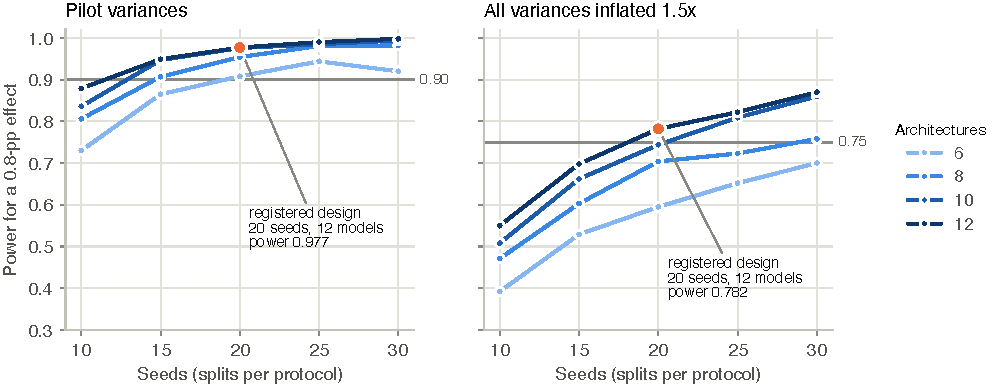
\includegraphics[width=\textwidth]{power.pdf}
\caption{Simulated power of the H1 model for a 0.8-pp effect (1,000 simulations per design).}
\label{r:fig:power}
\end{figure}

{\footnotesize
\setlength{\tabcolsep}{3.5pt}
\begin{longtable}{llrrrrr}
\caption{Simulated power (1,000 simulations per cell) of the registered H1 model for a 0.8-pp effect, by variance scale, number of architectures, and number of seeds.}\label{r:tab:power}\\
\toprule
Variance & Archs & 10 seeds & 15 seeds & 20 seeds & 25 seeds & 30 seeds \\
\midrule
\endfirsthead
\toprule
Variance & Archs & 10 seeds & 15 seeds & 20 seeds & 25 seeds & 30 seeds \\
\midrule
\endhead
\bottomrule
\endfoot
1$\times$ & 6 & 0.730 & 0.865 & 0.908 & 0.944 & 0.920 \\
1$\times$ & 8 & 0.806 & 0.907 & 0.954 & 0.981 & 0.982 \\
1$\times$ & 10 & 0.836 & 0.947 & 0.976 & 0.985 & 0.994 \\
1$\times$ & 12 & 0.879 & 0.949 & 0.977 & 0.990 & 0.998 \\
1.5$\times$ & 6 & 0.392 & 0.529 & 0.595 & 0.652 & 0.700 \\
1.5$\times$ & 8 & 0.471 & 0.603 & 0.704 & 0.723 & 0.758 \\
1.5$\times$ & 10 & 0.508 & 0.662 & 0.744 & 0.809 & 0.860 \\
1.5$\times$ & 12 & 0.550 & 0.698 & 0.782 & 0.822 & 0.870 \\
\end{longtable}
}


\chapter{The designs in detail}
\label{r:ch:designs}

\begin{figure}[H]
\centering
\begin{adjustbox}{max width=\textwidth}
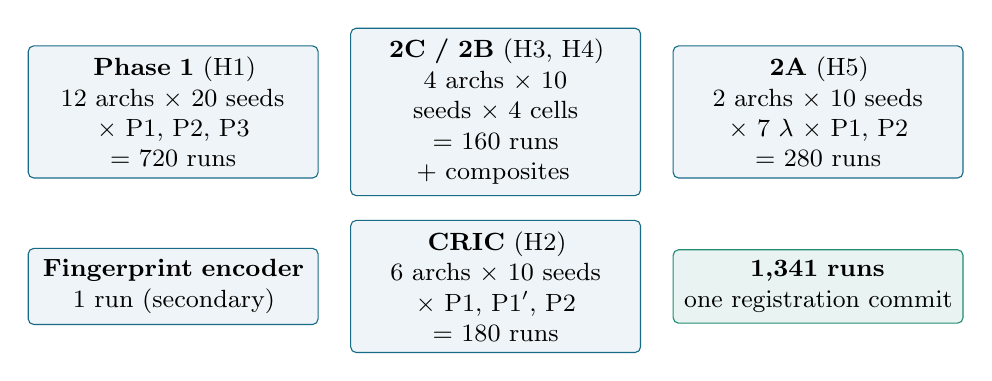
\begin{tikzpicture}[node distance=3mm and 4mm]
\node[box=34mm] (p1) {\textbf{Phase 1} (H1)\\12 archs $\times$ 20 seeds $\times$ P1, P2, P3\\= 720 runs};
\node[box=34mm, right=of p1] (fc) {\textbf{2C / 2B} (H3, H4)\\4 archs $\times$ 10 seeds $\times$ 4 cells\\= 160 runs + composites};
\node[box=34mm, right=of fc] (gr) {\textbf{2A} (H5)\\2 archs $\times$ 10 seeds $\times$ 7 $\lambda$ $\times$ P1, P2\\= 280 runs};
\node[box=34mm, below=of fc] (cr) {\textbf{CRIC} (H2)\\6 archs $\times$ 10 seeds $\times$ P1, P1$'$, P2\\= 180 runs};
\node[box=34mm, left=of cr] (fp) {\textbf{Fingerprint encoder}\\1 run (secondary)};
\node[done=34mm, right=of cr] (tot) {\textbf{1,341 runs}\\one registration commit};
\end{tikzpicture}
\end{adjustbox}
\caption{The registered Study 2 run matrix. P1-prime equals P1 byte for byte on every SIPaKMeD seed (P2 always has
exactly 810 test crops), so it needed no separate SIPaKMeD runs.}
\label{r:fig:study2-matrix}
\end{figure}


\section{Splits}

P1 is a stratified 80:20 crop split; P2 a parent-disjoint split taken from \texttt{StratifiedGroupKFold} as the fold
whose test size is closest to 810 crops; P3 the same on near-duplicate component groups. For every SIPaKMeD seed P2 has
exactly 810 test crops, so P1-prime (a P1 split resampled to P2's size) is byte-identical to P1 and was not trained
separately. For CRIC, P1-prime differs from P1 by 2--11 training cells and was trained.

\section{Architectures}

{\footnotesize
\setlength{\tabcolsep}{3.5pt}
\begin{longtable}{llp{4.6cm}rr}
\caption{The twelve Study 2 backbones: penultimate feature dimension, ImageNet weights, and mean Phase 1 training and total minutes per run.}\label{r:tab:archs}\\
\toprule
Architecture & Dim & Weights & Train min & Total min \\
\midrule
\endfirsthead
\toprule
Architecture & Dim & Weights & Train min & Total min \\
\midrule
\endhead
\bottomrule
\endfoot
ResNet-18 & 512 & ResNet18\_\allowbreak{}Weights.\allowbreak{}IMAGENET1K\_\allowbreak{}V1 & 0.85 & 0.87 \\
ResNet-50 & 2048 & ResNet50\_\allowbreak{}Weights.\allowbreak{}IMAGENET1K\_\allowbreak{}V2 & 2.60 & 2.64 \\
DenseNet-121 & 1024 & DenseNet121\_\allowbreak{}Weights.\allowbreak{}IMAGENET1K\_\allowbreak{}V1 & 3.25 & 3.29 \\
EfficientNet-B0 & 1280 & EfficientNet\_\allowbreak{}B0\_\allowbreak{}Weights.\allowbreak{}IMAGENET1K\_\allowbreak{}V1 & 1.78 & 1.80 \\
MobileNet-V2 & 1280 & MobileNet\_\allowbreak{}V2\_\allowbreak{}Weights.\allowbreak{}IMAGENET1K\_\allowbreak{}V2 & 1.45 & 1.48 \\
ViT-B/16 & 768 & ViT\_\allowbreak{}B\_\allowbreak{}16\_\allowbreak{}Weights.\allowbreak{}IMAGENET1K\_\allowbreak{}V1 & 9.09 & 9.17 \\
ConvNeXt-T & 768 & ConvNeXt\_\allowbreak{}Tiny\_\allowbreak{}Weights.\allowbreak{}IMAGENET1K\_\allowbreak{}V1 & 5.15 & 5.21 \\
Swin-T & 768 & Swin\_\allowbreak{}T\_\allowbreak{}Weights.\allowbreak{}IMAGENET1K\_\allowbreak{}V1 & 4.61 & 4.66 \\
RegNetY-1.6GF & 888 & RegNet\_\allowbreak{}Y\_\allowbreak{}1\_\allowbreak{}6GF\_\allowbreak{}Weights.\allowbreak{}IMAGENET1K\_\allowbreak{}V2 & 2.47 & 2.50 \\
EfficientNetV2-S & 1280 & EfficientNet\_\allowbreak{}V2\_\allowbreak{}S\_\allowbreak{}Weights.\allowbreak{}IMAGENET1K\_\allowbreak{}V1 & 3.46 & 3.50 \\
MaxViT-T & 512 & MaxVit\_\allowbreak{}T\_\allowbreak{}Weights.\allowbreak{}IMAGENET1K\_\allowbreak{}V1 & 7.76 & 7.86 \\
DINOv2 ViT-S/14 & 384 & timm:vit\_\allowbreak{}small\_\allowbreak{}patch14\_\allowbreak{}dinov2.\allowbreak{}lvd142m & 4.08 & 4.13 \\
\end{longtable}
}


\section{2C: leakage at matched diversity}

\begin{figure}[H]
\centering
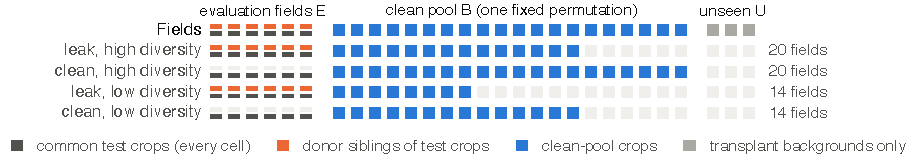
\includegraphics[width=\textwidth]{design.pdf}
\caption{The 2C factorial for one seed: one common test set; leak cells add the evaluation fields' sibling crops, clean
cells use other fields; within a diversity level crop and field counts are identical, and low-diversity field sets are
nested in high-diversity ones.}
\label{r:fig:design}
\end{figure}

For each seed and class, 30\% of fields with at least two crops are evaluation fields; half of each one's crops (rounded
down) form the common test set (about 527 crops) and the rest are its donor siblings. Six fields per class with at least
three crops are reserved as unseen background donors for 2B. Each training set holds exactly 220 crops per class. The
clean cells draw from non-evaluation fields along one fixed permutation; the leak cells replace the last $|E|$ fields of
that permutation with the evaluation fields' donor siblings; the low-diversity cells use the first 70\% of the
permutation. High-diversity cells therefore contain 720 distinct fields and low-diversity cells 504. Every test crop
has a training sibling in the leak cells (2.0 on average at high diversity, 3.0 at low) and none in the clean cells. A
240-crop budget was infeasible for seed 307 and for 10 of 100 unrelated seeds, so 220 was chosen before any training;
it was feasible for 100 of 100.

\section{2B: counterfactual background transplants}

\begin{figure}[H]
\centering
\begin{adjustbox}{max width=\textwidth}
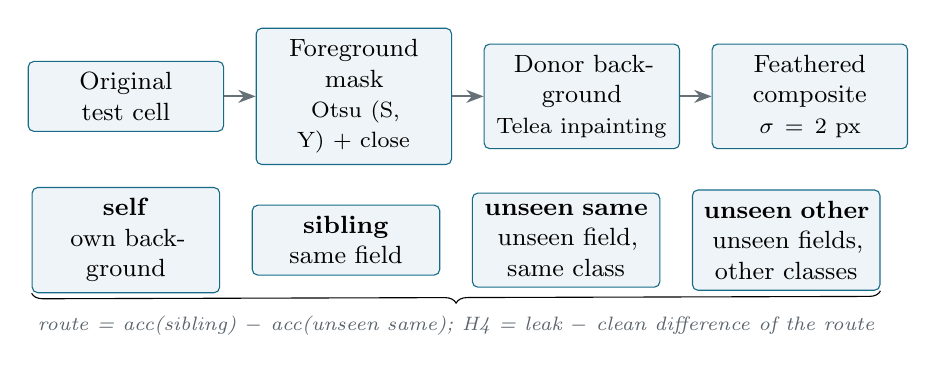
\begin{tikzpicture}[node distance=3mm and 4mm]
\node[box=22mm] (orig) {Original test cell};
\node[box=22mm, right=of orig] (mask) {Foreground mask\\\footnotesize Otsu (S, Y) + close};
\node[box=22mm, right=of mask] (inp) {Donor background\\\footnotesize Telea inpainting};
\node[box=22mm, right=of inp] (comp) {Feathered composite\\\footnotesize $\sigma=2$ px};
\node[box=21mm, below=7mm of orig] (self) {\textbf{self}\\own background};
\node[box=21mm, right=of self] (sib) {\textbf{sibling}\\same field};
\node[box=21mm, right=of sib] (same) {\textbf{unseen same}\\unseen field, same class};
\node[box=21mm, right=of same] (other) {\textbf{unseen other}\\unseen fields, other classes};
\draw[flow] (orig) -- (mask); \draw[flow] (mask) -- (inp); \draw[flow] (inp) -- (comp);
\draw[decorate,decoration={brace,amplitude=4pt,mirror}] (self.south west) -- (other.south east)
  node[midway, below=5pt, note] {route = acc(sibling) $-$ acc(unseen same); H4 = leak $-$ clean difference of the route};
\end{tikzpicture}
\end{adjustbox}
\caption{The 2B counterfactual background transplants. The \emph{self} condition measures seam and inpainting artifacts;
every contrast compares conditions that share them.}
\label{r:fig:transplant-diagram}
\end{figure}


\section{2A: adversarial fingerprint suppression}

\begin{figure}[H]
\centering
\begin{adjustbox}{max width=\textwidth}
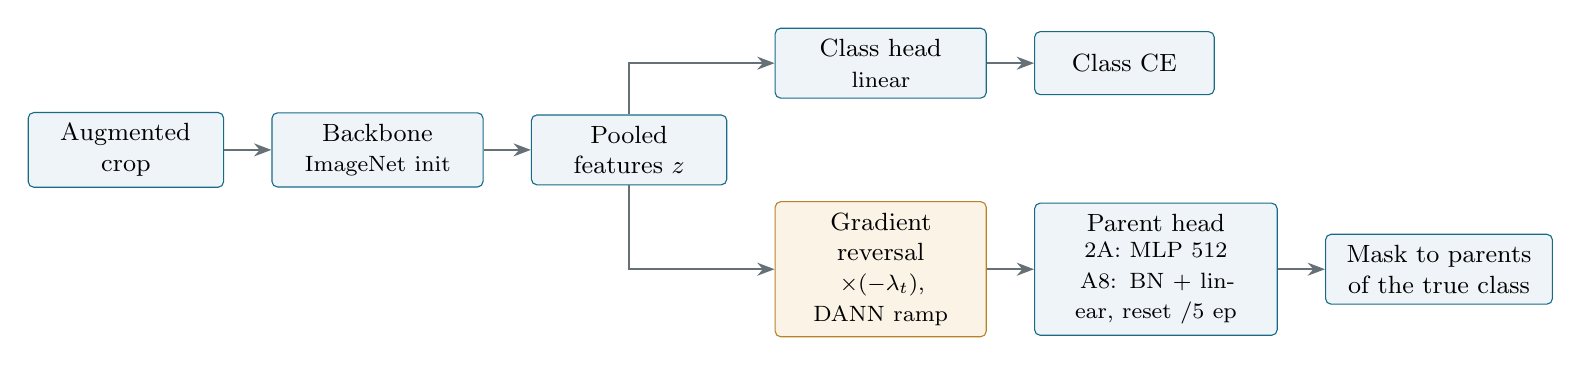
\begin{tikzpicture}[node distance=4mm and 6mm]
\node[box=22mm] (x) {Augmented crop};
\node[box=24mm, right=of x] (bb) {Backbone\\\footnotesize ImageNet init};
\node[box=22mm, right=of bb] (f) {Pooled features $z$};
\node[box=24mm, above right=2mm and 6mm of f] (head) {Class head\\\footnotesize linear};
\node[gold=24mm, below right=2mm and 6mm of f] (grl) {Gradient reversal\\\footnotesize $\times(-\lambda_t)$, DANN ramp};
\node[box=28mm, right=of grl] (adv) {Parent head\\\footnotesize 2A: MLP 512\\\footnotesize A8: BN + linear, reset /5 ep};
\node[box=26mm, right=of adv] (mask) {Mask to parents of the true class};
\node[box=20mm, right=of head] (ce) {Class CE};
\draw[flow] (x) -- (bb); \draw[flow] (bb) -- (f); \draw[flow] (f) |- (head); \draw[flow] (f) |- (grl);
\draw[flow] (grl) -- (adv); \draw[flow] (adv) -- (mask); \draw[flow] (head) -- (ce);
\end{tikzpicture}
\end{adjustbox}
\caption{The adversarial suppression arms. The parent adversary only competes among parents of the sample's own class,
so suppressing it never requires removing class information. Study 2 (2A) used a two-layer MLP; Amendment 8 (F7) used a
probe-matched head (per-feature standardisation and one linear layer, its own optimiser at $10^{-3}$, re-initialised every
five epochs) so that features could not hide parent identity from it while leaving it readable by a linear probe.}
\label{r:fig:adversary}
\end{figure}


The maximum reversal coefficient followed the DANN ramp $\lambda\,(2/(1+e^{-10p})-1)$ over training progress $p$, with
$\lambda\in\{0, 0.01, 0.03, 0.1, 0.3, 1, 3\}$. Recoverability $R$ is the within-class field-identification accuracy of a
multinomial logistic regression (C = 1, standardised features) on frozen features of the balanced 424-field probe split
(two fitting and two evaluation crops per field). The \emph{regime} is the set of $\lambda$ whose mean P2 accuracy stays
within 1~pp of $\lambda=0$; the \emph{manipulation check} requires $R$ at the strongest in-regime $\lambda$ to fall by at
least a quarter of its above-floor baseline.

\section{CRIC}

CRIC cells are $100\times100$ windows centred on the published nucleus coordinates (shifted inward at image borders) of
the 400 Figshare slide images, whose MD5 and SHA-256 were verified (\artifact{data_manifests/cric_images_verified.json}).
Six Bethesda classes; ResNet-18, ResNet-50, DenseNet-121, EfficientNet-B0, ConvNeXt-T, ViT-B/16; P1, P1-prime, P2; ten
seeds.

\chapter{Structure before training}
\label{r:ch:structure}

For a parent with $k$ crops allocated independently with test fraction $q$, the parent straddles the split with
probability $1-(1-q)^k-q^k$; a test crop has a training sibling with probability $1-q^{k-1}$ and $(1-q)(k-1)$ training
siblings on average; and the ratio of distinct training parents between a crop-level and a parent-level split of equal
size is $\sum_j\{1-q^{k_j}\}/\{(1-q)m\}$ for $m$ parents. Class--parent dependence is the mutual information between
parent and class divided by the class entropy. \texttt{cytofair risk-report} computes all of them from any crop-to-parent
table (\artifact{src/cytofair/risk.py}).

{\scriptsize
\setlength{\tabcolsep}{3.5pt}
\begin{longtable}{lrrrrrrrr}
\caption{\texttt{cytofair risk-report} closed forms for the four datasets at a 20\% test fraction: crops per parent, expected straddle and sibling rates (percent), siblings per test crop, training-diversity ratio, and class--parent dependence (fraction of class entropy explained by the parent).}\label{r:tab:risk}\\
\toprule
Dataset & Obs. & Parents & Obs./parent & Straddle & Test w/ sibling & Siblings & Diversity & Class dep. \\
\midrule
\endfirsthead
\toprule
Dataset & Obs. & Parents & Obs./parent & Straddle & Test w/ sibling & Siblings & Diversity & Class dep. \\
\midrule
\endhead
\bottomrule
\endfoot
SIPaKMeD & 4,049 & 966 & 4.19 & 44.8 & 91.7 & 5.16 & 1.176 & 1.000 \\
Cx22 & 1,320 & 514 & 2.57 & 33.9 & 83.6 & 1.95 & 1.164 & -- \\
CRIC & 11,534 & 400 & 28.84 & 94.9 & 100.0 & 35.56 & 1.250 & 0.676 \\
Herlev & 917 & 917 & 1.00 & 0.0 & 0.0 & 0.00 & 1.000 & 1.000 \\
\end{longtable}
}


\begin{figure}[H]
\centering
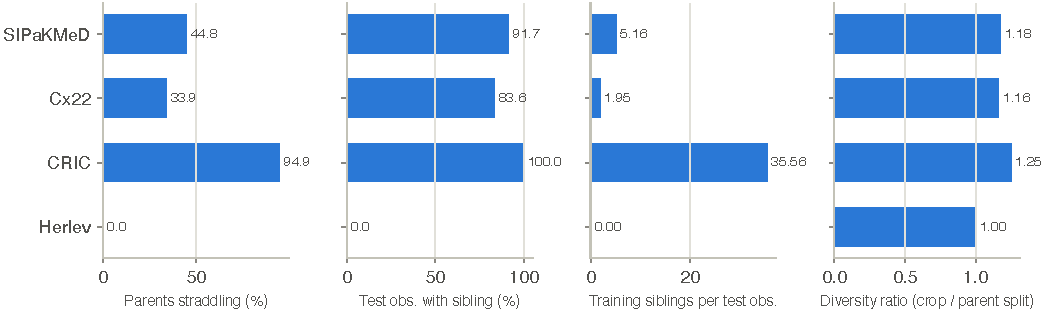
\includegraphics[width=\textwidth]{structure.pdf}
\caption{Closed-form structural exposure of the four datasets to a random 80:20 crop split.}
\label{r:fig:structure}
\end{figure}

Under five random P1 splits, the share of test observations sharing at least one source pixel with a training
observation was \RecOverlapSip\% for SIPaKMeD, \RecOverlapCric\% for CRIC, and \RecOverlapCx\% for Cx22
(\artifact{results/study2/structural/literal_overlap_p1.csv}). CRIC is exposed on every measure: 29 cells per slide image,
essentially every test cell with a training sibling, and slide identity explaining two thirds of the class entropy.
That is the structure that predicted, before training, that CRIC's inflation would be the largest.

\part{Engineering and Execution}

\chapter{The host, the data path, and the training stack}
\label{r:ch:host}

\section{The host and its constraints}

All Study~2 and Amendment~8 computation ran on one shared server (\texttt{node1}) with eight NVIDIA RTX A6000 GPUs
(49~GB each). It has no job scheduler; work runs directly on the login node. The operating rules for the project were:
never more than four GPUs at once, check for vacant GPUs first, keep data that feeds GPUs off the shared network
filesystem, use the fast local disk and vacate it afterwards.

\begin{longtable}{p{0.26\textwidth}p{0.64\textwidth}}
\caption{Host constraints discovered or imposed, and the response to each.}\label{r:tab:host}\\
\toprule
Constraint & Consequence and response \\
\midrule
\endfirsthead
\toprule
Constraint & Consequence and response \\
\midrule
\endhead
\bottomrule
\endfoot
Four GPUs at most & Study~2 used GPUs 0, 3, 4, 5 (GPUs 1 and 2 were in use by another user); Amendment~8 used 4--7 after
another user started jobs on 0--3 twenty-five minutes before launch. The scheduler refuses more than four. \\
Four CPU cores per user & Found during Study~2 preparation: the per-user cgroup quota is 400\% (four cores) on a
128-core machine. The power simulation ran far slower than its core count suggested, a data-loader benchmark was invalid,
and per-image augmentation in loader workers could not feed even one GPU. This is very likely the ``host bottleneck''
recorded in Study~1 (Chapter~\ref{s1:ch:ch13_execution_lifecycle_failures_and_demotiv}). Response: decode crops once into
caches, upload them to the GPU, augment there (Section~\ref{r:ch:gpuaug}), keep CPU threads low, and run heavy CPU
analyses on a workstation. \\
\texttt{/scratch} not writable & All node-local work used \texttt{/tmp/rchethan1\_cytofair} (the 192~GB root partition
shared with the operating system) and \texttt{/dev/shm}; a disk guard keeps 40~GB free. \\
Slow network home & The NFS home can stall under load; a recursive search over it had to be stopped early in Study~2
preparation. Rule adopted: only static artifacts go there, and copies are single bandwidth-limited streams. \\
Shared GPUs & Other users' jobs can appear at any time. The scheduler checks each GPU's memory before launching
(at most 30,000~MiB in use), and an infrastructure failure caused by another process does not count as a retry
(Amendment~7). \\
No scheduler & Background controllers launched with \texttt{setsid nohup} and detached from the SSH session; a status
file records every running task, completion, and failure. \\
\end{longtable}

\section{The data path}
\label{r:ch:datapath}

\subsection{Provenance to splits}

Every split is derived from the provenance maps of Study~1 (\artifact{provenance/*.parquet}), whose recovery and
verification are described in Part~II. \texttt{cytofair study2-design} writes every Study~2 split, factorial design,
transplant plan, and the probe split with SHA-256 hashes into \artifact{splits/study2/study2_split_manifest.csv};
\texttt{cytofair followup-design} does the same for Amendment~8 (\artifact{splits/study2/followup/}). Trainers hash the
split file before use and refuse a mismatch.

\subsection{Packed crop caches}

Decoding thousands of small BMP and PNG files on four cores is slow, and reading them from the network home is
unreliable. Each image set is therefore packed once into a cache on the node-local disk: one \texttt{uint8} array of all
pixels (\texttt{\{name\}\_pixels.npy}, memory-mapped), an index (\texttt{\{name\}\_index.parquet}) with each crop's offset,
height, width, and the SHA-256 of its pixels, and a manifest with the SHA-256 of both files. A cache is verified on load;
a hash mismatch stops the run.

\begin{longtable}{p{0.3\textwidth}p{0.18\textwidth}p{0.45\textwidth}}
\caption{Caches used by Study 2 and Amendment 8 (hashes in Appendix~\ref{r:app:hashes}).}\label{r:tab:caches}\\
\toprule
Cache & Images & Content \\
\midrule
\endfirsthead
\bottomrule
\endfoot
\texttt{sipakmed} & 4,049 & every SIPaKMeD crop \\
\texttt{cric} & 11,534 & $100\times100$ windows around every CRIC nucleus \\
\texttt{transplant\_seed*} (10) & 4,096--4,400 each & 2B composites of each seed's common test set \\
\texttt{sipakmed\_masked} & 4,049 & background set to the ImageNet mean (F3) \\
\texttt{sipakmed\_reinhard50/100} & 4,049 each & Reinhard normalisation at strength 0.5 and 1 (F6) \\
\texttt{ablation\_seed*} (10) & six per test crop & the F2 carrier ablations \\
\end{longtable}

\section{The GPU-resident input path}
\label{r:ch:gpuaug}

\begin{figure}[H]
\centering
\begin{adjustbox}{max width=\textwidth}
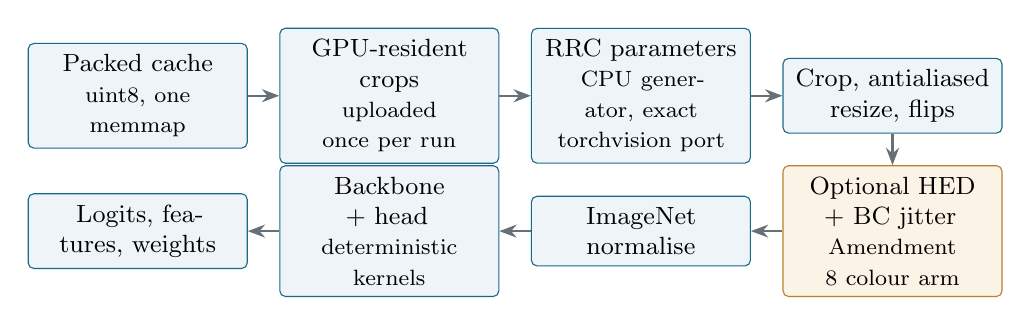
\begin{tikzpicture}[node distance=4mm and 4mm]
\node[box=25mm] (cache) {Packed cache\\\footnotesize uint8, one memmap};
\node[box=25mm, right=of cache] (gpu) {GPU-resident crops\\\footnotesize uploaded once per run};
\node[box=25mm, right=of gpu] (params) {RRC parameters\\\footnotesize CPU generator, exact torchvision port};
\node[box=25mm, right=of params] (crop) {Crop, antialiased resize, flips};
\node[gold=25mm, below=of crop] (color) {Optional HED + BC jitter\\\footnotesize Amendment 8 colour arm};
\node[box=25mm, left=of color] (norm) {ImageNet normalise};
\node[box=25mm, left=of norm] (model) {Backbone + head\\\footnotesize deterministic kernels};
\node[box=25mm, left=of model] (out) {Logits, features, weights};
\draw[flow] (cache) -- (gpu); \draw[flow] (gpu) -- (params); \draw[flow] (params) -- (crop);
\draw[flow] (crop) -- (color); \draw[flow] (color) -- (norm); \draw[flow] (norm) -- (model); \draw[flow] (model) -- (out);
\end{tikzpicture}
\end{adjustbox}
\caption{The GPU-resident training input path. The host allowed four CPU cores per user, which made per-image PIL
augmentation in data-loader workers the bottleneck; moving the registered augmentation onto the GPU removed it
while sampling exactly the same crop geometry as torchvision for the same random stream.}
\label{r:fig:gpu-augment}
\end{figure}


The registered augmentation is \texttt{RandomResizedCrop(224, scale 0.8--1.0, ratio 3/4--4/3)}, horizontal and vertical
flips, and ImageNet normalisation. \artifact{src/cytofair/gpu_augment.py} keeps every crop of a split on the GPU as a
\texttt{uint8} tensor and draws crop parameters with an exact port of torchvision's \texttt{RandomResizedCrop.get\_params}
from an explicit CPU generator, including the float32 exponential torchvision uses for the aspect ratio. A unit test
compares the sampled geometry with torchvision's for four image shapes and 25 seeds each and requires identity. Resizing
uses antialiased bilinear interpolation, PyTorch's implementation of PIL's filter, which can differ from PIL by uint8
rounding. The Amendment~8 colour arm adds HED optical-density jitter and brightness/contrast jitter, drawn from the same
generator after the geometry, so runs without colour augmentation reproduce the registered random stream exactly.

\section{Determinism}
\label{r:ch:determinism}

Every run sets cuDNN deterministic mode, disables cuDNN benchmarking, calls
\path{torch.use_deterministic_algorithms(True, warn_only=True)}, and sets \texttt{CUBLAS\_WORKSPACE\_CONFIG=:4096:8}.
During smoke tests ViT-B/16 raised a warning that the memory-efficient attention backward pass is non-deterministic; the
flash, memory-efficient, and cuDNN attention kernels were disabled in favour of the math kernel, and two identical ViT
runs then produced bitwise-identical logits. The follow-up evaluation code avoids \texttt{index\_add\_} (non-deterministic
on CUDA) by computing group sums as one-hot matrix products.

Final weights are stored in float16 to halve their size. Re-evaluating the saved Phase~1 checkpoints reproduced the
recorded test accuracy exactly for 418 of 480 models; 56 differed by one test crop and six by two or three crops out of
810, all from float16 rounding. Every follow-up comparison is made within one re-evaluation, so this does not bias any
registered contrast.

\section{What every run leaves behind}
\label{r:ch:artifacts}

\artifact{src/cytofair/train_study2.py} writes, for every run:
\begin{itemize}[leftmargin=1.6em]
\item a JSON record with the dataset, protocol, architecture, seed, accuracy, macro-F1, balanced accuracy, NLL, 15-bin ECE,
the confusion matrix, train and test crop and parent counts, the fraction of test crops with a training parent, the
recipe and augmentation, adversary settings, the split file and semantic hashes, cache hashes, the git commit, GPU,
start and end times, runtime metadata, a per-epoch history, and the path and SHA-256 of every artifact;
\item per-crop test logits (Parquet), float16 final weights, penultimate features of the 1,696 probe crops (NPZ), and
logits for any registered extra evaluation set (the 2B composites).
\end{itemize}
The follow-up evaluation tasks write comparable records (\artifact{src/cytofair/followup_eval.py}), verifying each
checkpoint's hash before loading it. The exported tables in \artifact{results/study2/run_records} keep every field the
record plots, including all \RecEpochs\ epoch histories.

\chapter{Scheduling, execution, and archiving}
\label{r:ch:scheduler}

\section{Scheduling, failure handling, and collection}

\begin{figure}[H]
\centering
\begin{adjustbox}{max width=\textwidth}
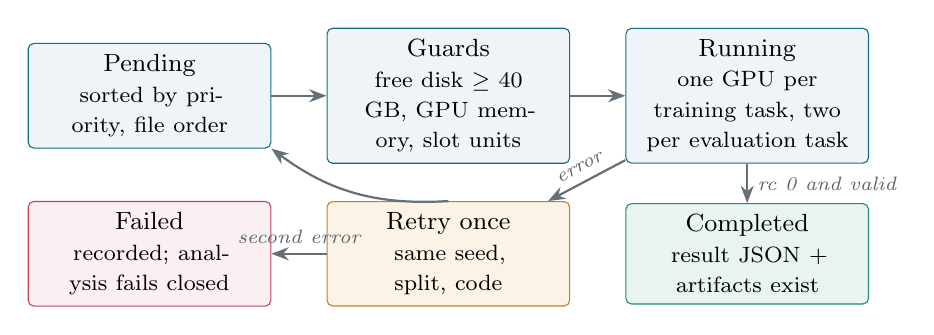
\begin{tikzpicture}[node distance=5mm and 7mm]
\node[box=28mm] (pending) {Pending\\\footnotesize sorted by priority, file order};
\node[box=28mm, right=of pending] (guard) {Guards\\\footnotesize free disk $\geq$ 40 GB, GPU memory, slot units};
\node[box=28mm, right=of guard] (running) {Running\\\footnotesize one GPU per training task, two per evaluation task};
\node[done=28mm, below=of running] (done) {Completed\\\footnotesize result JSON + artifacts exist};
\node[gold=28mm, left=of done] (retry) {Retry once\\\footnotesize same seed, split, code};
\node[bad=28mm, left=of retry] (fail) {Failed\\\footnotesize recorded; analysis fails closed};
\draw[flow] (pending) -- (guard); \draw[flow] (guard) -- (running);
\draw[flow] (running) -- node[note, right]{rc 0 and valid} (done);
\draw[flow] (running) -- node[note, above, sloped]{error} (retry);
\draw[flow] (retry) -- node[note, above]{second error} (fail);
\draw[flow] (retry.north) to[bend left=20] (pending.south east);
\end{tikzpicture}
\end{adjustbox}
\caption{The resumable scheduler (\texttt{scripts/\allowbreak study2/\allowbreak launch\_matrix.py}). A task whose valid result already exists is
skipped on restart, so the controller can be relaunched after any interruption without duplicating a run.}
\label{r:fig:launcher}
\end{figure}


A task is a JSON line naming its command, the result file that proves completion, a priority, the GPU share it needs,
and an \texttt{expect} block of fields its result must carry (dataset, protocol, architecture, seed, split hash, and for
the follow-up arms the cache, colour augmentation, and adversary). \artifact{scripts/study2/build_tasks.py} wrote the
1,341 Study~2 tasks and \artifact{scripts/study2/build_followup_tasks.py} the 1,580 follow-up tasks; both sets are
committed and hashed. Training tasks took a whole GPU; evaluation-only tasks took half, so two ran per GPU.

The collectors (\artifact{analysis/study2/collect_runs.py}, \artifact{analysis/study2/followup/prepare_followup.py})
require exactly one valid result per registered task whose recorded fields match its \texttt{expect} block; anything
missing, duplicated, or mismatched is listed and the analysis stops. \texttt{--allow-incomplete} produces progress reports
only. Under Amendment~7, adversarial runs whose every attempt ended in a non-finite loss are recognised from their logs and
recorded as diverged rather than missing. Neither matrix had a failure, retry, or divergence.

\section{Execution}
\label{r:ch:execution}

\subsection{Smoke tests}

Before each registration, short runs exercised every code path on splits that cannot reveal a registered contrast: P1
splits only for Study~2; leak cells, single P1 runs, and single evaluation tasks for Amendment~8
(Table~\ref{r:tab:ledger-smoke}). Their metrics were checked only for finiteness and integrity (for example, that a
re-evaluated checkpoint reproduces its recorded accuracy).

\subsection{The two matrices}

\begin{figure}[H]
\centering
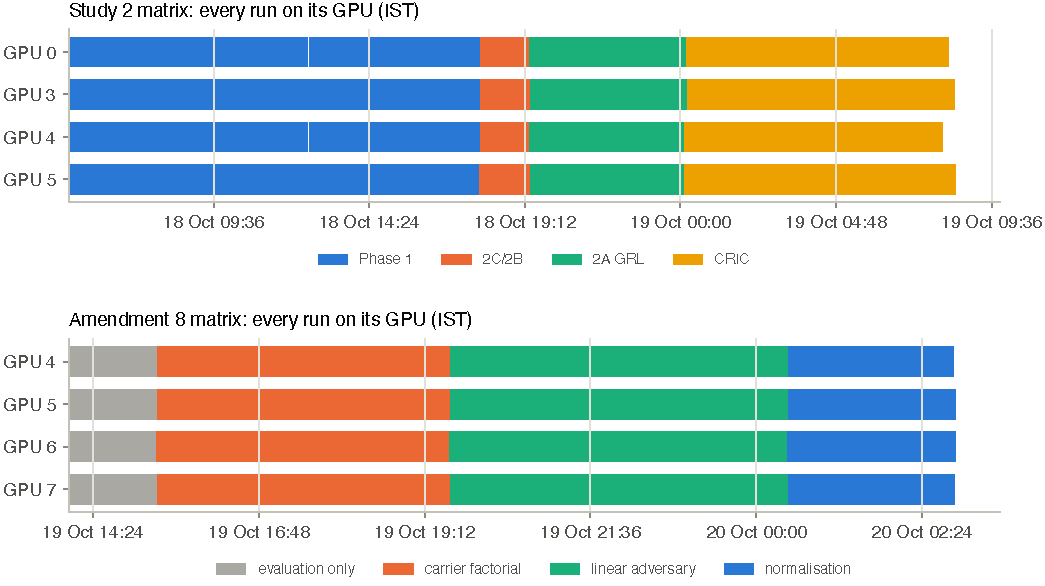
\includegraphics[width=\textwidth]{gpu_schedule.pdf}
\caption{Every run of both matrices on its GPU, from the start and end times in the run records (evaluation tasks from
the controller log). The arms ran in priority order; white gaps are launch overhead.}
\label{r:fig:gpu-schedule}
\end{figure}

{\footnotesize
\setlength{\tabcolsep}{3.5pt}
\begin{longtable}{lrrrll}
\caption{Compute ledger of every Study 2 and Amendment 8 arm (node1, NVIDIA RTX A6000; times in IST). GPU-hours are summed per-run elapsed time; runs shared four GPUs.}\label{r:tab:compute}\\
\toprule
Arm & Runs & Mean min & GPU-h & First start & Last finish \\
\midrule
\endfirsthead
\toprule
Arm & Runs & Mean min & GPU-h & First start & Last finish \\
\midrule
\endhead
\bottomrule
\endfoot
Study 2 Phase 1 (H1) & 720 & 3.9 & 47.1 & 18 Oct 05:07 & 18 Oct 17:50 \\
Study 2 2C/2B (H3, H4) & 160 & 2.0 & 5.4 & 18 Oct 17:48 & 18 Oct 19:21 \\
Study 2 2A (H5) & 280 & 3.9 & 18.2 & 18 Oct 19:20 & 19 Oct 00:12 \\
Study 2 CRIC (H2) & 180 & 10.7 & 32.0 & 19 Oct 00:06 & 19 Oct 08:28 \\
A8 carrier factorial (F3, F4) & 480 & 1.9 & 15.2 & 19 Oct 15:19 & 19 Oct 19:34 \\
A8 linear adversary (F7) & 300 & 3.7 & 18.5 & 19 Oct 19:33 & 20 Oct 00:27 \\
A8 stain normalisation (F6) & 160 & 3.4 & 9.1 & 20 Oct 00:27 & 20 Oct 02:52 \\
A8 ablations + Grad-CAM (F2) & 160 & 0.2 & 0.6 & 19 Oct 14:03 & 19 Oct 14:14 \\
A8 LEACE erasure (F5) & 480 & 0.8 & 6.5 & 19 Oct 14:13 & 19 Oct 15:19 \\
\end{longtable}
}


\begin{figure}[H]
\centering
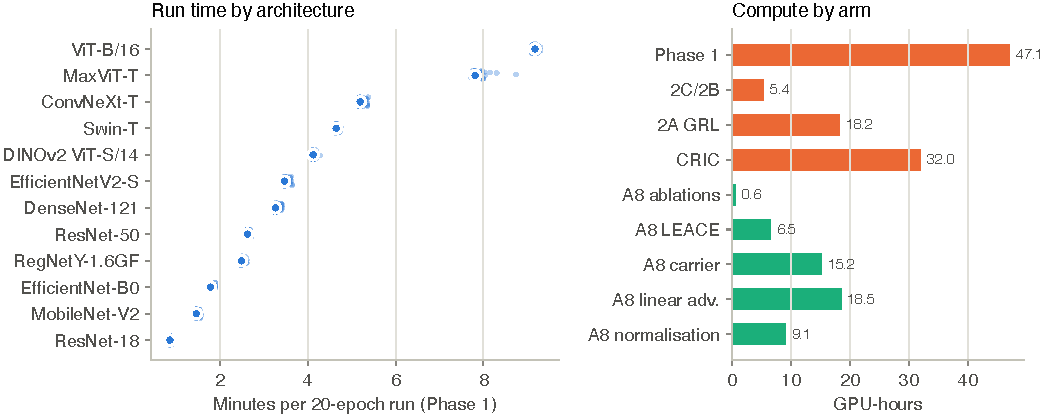
\includegraphics[width=\textwidth]{runtime.pdf}
\caption{Left: wall time of each Phase~1 run by architecture (dots) and its median (ring). Right: GPU-hours by arm.}
\label{r:fig:runtime}
\end{figure}

\subsection{Software}

{\footnotesize
\setlength{\tabcolsep}{3.5pt}
\begin{longtable}{lp{11cm}}
\caption{Software and hardware recorded in every training run.}\label{r:tab:software}\\
\toprule
Component & Version \\
\midrule
\endfirsthead
\toprule
Component & Version \\
\midrule
\endhead
\bottomrule
\endfoot
python & 3.13.9 \\
torch & 2.9.0+cu128 \\
torchvision & 0.24.0+cu128 \\
timm & 1.0.22 \\
cuda & 12.8 \\
cudnn & 91002 \\
cuda\_device & NVIDIA RTX A6000 \\
numpy & 2.5.2 \\
pandas & 3.0.5 \\
scipy & 1.18.1 \\
scikit\_learn & 1.9.0 \\
opencv & 5.0.0 \\
pillow & 12.3.0 \\
platform & Linux-4.18.0-372.9.1.el8.x86\_64-x86\_64-with-glibc2.28 \\
cublas\_workspace\_config & :4096:8 \\
\end{longtable}
}


\section{Archiving and vacating}
\label{r:ch:archive}

\begin{figure}[H]
\centering
\begin{adjustbox}{max width=\textwidth}
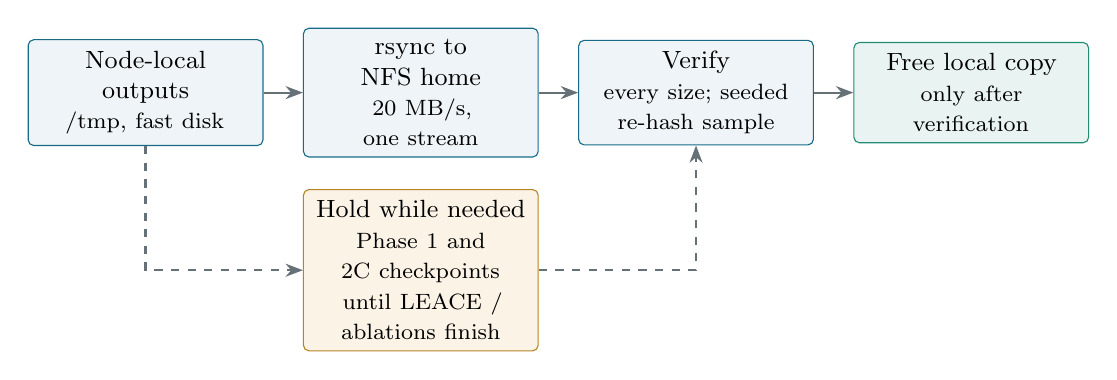
\begin{tikzpicture}[node distance=4mm and 5mm]
\node[box=27mm] (local) {Node-local outputs\\\footnotesize /tmp, fast disk};
\node[box=27mm, right=of local] (rsync) {rsync to NFS home\\\footnotesize 20 MB/s, one stream};
\node[box=27mm, right=of rsync] (verify) {Verify\\\footnotesize every size; seeded re-hash sample};
\node[done=27mm, right=of verify] (free) {Free local copy\\\footnotesize only after verification};
\node[gold=27mm, below=of rsync] (hold) {Hold while needed\\\footnotesize Phase 1 and 2C checkpoints until LEACE / ablations finish};
\draw[flow] (local) -- (rsync); \draw[flow] (rsync) -- (verify); \draw[flow] (verify) -- (free);
\draw[flow, dashed] (local) |- (hold); \draw[flow, dashed] (hold) -| (verify);
\end{tikzpicture}
\end{adjustbox}
\caption{Offloading and archiving. The network home is slow and can stall, so copies are single, bandwidth-limited
streams; nothing node-local is deleted until its archived copy has been verified.}
\label{r:fig:archive}
\end{figure}


The follow-up matrix would write about 52~GB of checkpoints into a 71~GB margin, so Study~2 checkpoints were moved to
the network home while it ran: the gradient-reversal and CRIC checkpoints first, then the 2C checkpoints once all 160
ablation tasks had finished, then the Phase~1 checkpoints once all 480 LEACE tasks had finished. Each experiment was
copied, every checkpoint's size compared, a seeded sample of fifty re-hashed against the hash in its run record, and only
then deleted locally. At the end, the follow-up outputs were copied and verified (3,580 artifacts, sizes all matching,
100 re-hashed), the remaining Study~2 outputs re-verified (4,000 artifacts, 200 re-hashed), and the node-local working
directory and shared-memory directory deleted. The archive (\texttt{\textasciitilde/cytofair\_study2\_archive}, 121~GB)
holds every run record, prediction, feature file, checkpoint, log, and status file.

\chapter{Errors, setbacks, and fixes}
\label{r:ch:errors}

Study~1's setbacks (the invalid first classification matrix, the MAnet numerical failure, and the host bottleneck) are
recorded in Chapter~\ref{s1:ch:ch13_execution_lifecycle_failures_and_demotiv}. Everything that went wrong afterwards is
listed here, including mistakes in tooling and in procedure; none changed a registered model, split, seed, or
endpoint.

{\small
\begin{longtable}{p{0.04\textwidth}p{0.26\textwidth}p{0.34\textwidth}p{0.23\textwidth}}
\caption{Every error and setback of Study 2 and Amendment 8, and its fix.}\label{r:tab:errors}\\
\toprule
\# & What went wrong & Fix & Effect on results \\
\midrule
\endfirsthead
\toprule
\# & What went wrong & Fix & Effect on results \\
\midrule
\endhead
\bottomrule
\endfoot
\multicolumn{4}{l}{\textbf{Study 2 preparation (before registration)}} \\
1 & No PDF text tools on the workstation & Python PDF libraries for reading and rendering & none \\
2 & A recursive search over the slow network home stalled & stopped; rule: never scan the network home & none \\
3 & \texttt{/scratch} not writable & node-local \texttt{/tmp} and \texttt{/dev/shm} & none \\
4 & Four-core CPU quota starved data loaders & GPU-resident augmentation; heavy CPU analysis off-host & none (exact port, unit-tested) \\
5 & Power script mis-named variance components; correlation on its $-1$ boundary & pattern matching; correlation set to 0 in the simulation & documented in the plan \\
6 & R: S4 slot read with \texttt{\$} in the protocol model & \texttt{@optinfo} & none \\
7 & R: tidy-evaluation operator inside base \texttt{subset} & explicit indexing & none \\
8 & 2C budget of 240 crops per class infeasible for some seeds & 220 crops, low/high ratio 0.70, feasible for 100/100 seeds & chosen before training \\
9 & pandas 3 read-only arrays; Pillow deprecation & copies; argument removed & none \\
10 & Non-deterministic attention backward (ViT) & math attention kernel only; bitwise repeat verified & none \\
11 & Lint findings, a wrong test expectation & fixed & none \\
12 & SSH launches hung on backgrounded command chains & \texttt{cd; setsid nohup \ldots\ \& disown} & none \\
13 & A shell wait loop did not split its input & explicit \texttt{read} & none \\
14 & No rule for diverged adversarial runs & Amendment~7, before any 2A run & none (no divergence) \\
\multicolumn{4}{l}{\textbf{Study 2 analysis}} \\
15 & One float16 probe-feature row overflowed (EfficientNetV2-S, one crop) & documented; no follow-up arm reads it & one crop in a descriptive measure \\
16 & A completion watcher never fired & replaced with a file-based check & none \\
\multicolumn{4}{l}{\textbf{Amendment 8}} \\
17 & Inference-mode tensors reused in autograd; non-deterministic \texttt{index\_add\_} & clone; one-hot matrix sums & caught in tests \\
18 & R summary object not serialisable to JSON & converted to a list & caught in dry run \\
19 & Remote \texttt{pgrep -f} matched its own command line & file-based completion checks & none \\
20 & Interim preparer crawled on a GPU busy with training & stopped; registered run on a free GPU & none \\
21 & \textbf{Preparer labelled standard carrier runs as colour-augmented} (\texttt{None} became a truthy NaN) & condition read from each run record; unit test; \textbf{Amendment~9} & script halted before output; no estimate seen \\
22 & An archive fetch included smoke checkpoints & refetched records only & none \\
23 & Dose figure plotted out-of-regime levels; labels overlapped & registered regimes only; layout fixed & presentation only \\
24 & Negative numbers typeset with a hyphen & typographic minus in the macro generator & presentation only \\
\end{longtable}
}

\begin{warningbox}{The one that mattered}
Error 21 is the only one that could have changed a reported number. The synthetic dry run had written condition
labels directly and so never exercised the preparer's labelling. The R script stopped at F4 because the contrast term was
missing, which exposed the bug before any output existed. The lesson recorded for the future: dry runs must go through
every stage of the real pipeline, not start from the tables that stage produces.
\end{warningbox}

\part{Study 2 Results}

\chapter{Overview of the registered outcome}
\label{r:ch:s2-overview}

All \RecStudyTwoRuns\ registered runs completed between \RecStudyTwoStart\ and \RecStudyTwoEnd~IST. None failed,
needed a retry, or diverged; every run was trained from the registration commit; every result matched its registered
split hash; and the collector reported no missing, duplicated, or mismatched task. The registered analysis
(\artifact{analysis/study2/run_all.sh}) ran once, on 19 October at 12:56.

\begin{longtable}{lp{0.42\textwidth}rrl}
\caption{The five registered Study 2 tests (H5 in pp of gap per pp of recoverability).}\label{r:tab:s2-verdicts}\\
\toprule
& Question & Estimate & Adjusted $p$ & Verdict \\
\midrule
\endfirsthead
\bottomrule
\endfoot
H1 & SIPaKMeD P1 $-$ P2 accuracy (primary, tested alone) & \HoneEst & \HoneP & \supported \\
H2 & CRIC P1 $-$ P2 accuracy & \HtwoEst & \HtwoPholm & \supported \\
H3 & Leakage at matched diversity (2C) & \HthreeEst & \HthreePholm & \supported \\
H4 & Own-context route through backgrounds (2B) & \HfourEst & \HfourPholm & \notsupported \\
H5 & Gap versus suppressed recoverability (2A) & \HfiveEst & \HfivePholm & \notsupported \\
\end{longtable}

Gate~A (H1 supported) means the inflation is reported as certified. Gate~B was ``murky'': H3 was supported but H4 was
not and H5 was not supported (one of two architectures failed its manipulation check). That is the result that motivated
Amendment~8.

\chapter{H1: crop-level splitting inflates SIPaKMeD accuracy}
\label{r:ch:h1}

\section{The registered test}

Mean test accuracy was \SipPOneAcc\% under P1 and \SipPTwoAcc\% under P2. The registered residual check flagged heavy
tails (residual skewness \RecHoneSkew, excess kurtosis \RecHoneKurt, Shapiro--Wilk $p$ \RecHoneShapiro), so, as registered,
the two-way cluster bootstrap is the primary inference: \HoneEst~pp (95\% interval \HoneBootLo--\HoneBootHi, bootstrap
$p$ \HoneBootP). Every sensitivity analysis agrees (Table~\ref{r:tab:sensitivity}): the mixed model gives the same
estimate with Satterthwaite $df=\HoneDf$ and $p$ \HoneKRp\ under Kenward--Roger, the seed-level sign-flip test gives $p$
\HoneSignFlipP, and the binomial mixed model a log odds ratio of \HoneGlmmLogOR\ ($p$ \HoneGlmmP).

\begin{figure}[H]
\centering
\begin{adjustbox}{max width=\textwidth}
\begin{tikzpicture}[node distance=5mm and 7mm]
\node[box=30mm] (fit) {Fit H1 model\\\footnotesize REML, bobyqa};
\node[gold=30mm, right=of fit] (conv) {Converged?\\\footnotesize singular accepted};
\node[box=30mm, right=of conv] (simp) {Simplify\\\footnotesize uncorrelated slope, then no seed intercept};
\node[gold=30mm, below=of conv] (assume) {Residual $|$skew$|>1$ or excess kurtosis $>3$?};
\node[done=30mm, left=of assume] (lmm) {Primary: Satterthwaite $t$-test};
\node[done=30mm, right=of assume] (boot) {Primary: two-way cluster bootstrap};
\node[box=95mm, below=6mm of assume] (sens) {Always reported: Kenward--Roger, binomial GLMM, seed sign-flip, bootstrap, per-architecture differences};
\draw[flow] (fit) -- (conv); \draw[flow] (conv) -- node[note, above]{no} (simp); \draw[flow] (simp.north) to[bend right=25] (fit.north);
\draw[flow] (conv) -- node[note, right]{yes} (assume); \draw[flow] (assume) -- node[note, above]{no} (lmm);
\draw[flow] (assume) -- node[note, above]{yes} (boot); \draw[flow] (assume) -- (sens);
\node[note, below=1mm of boot, text width=34mm] {Study 2: skew \RecHoneSkew, kurtosis \RecHoneKurt\ $\Rightarrow$ bootstrap};
\end{tikzpicture}
\end{adjustbox}
\caption{The registered H1 decision path. The residual check fired, so the cluster bootstrap became the primary inference
exactly as registered; every other method gave the same answer.}
\label{r:fig:h1-decision}
\end{figure}


\begin{figure}[H]
\centering
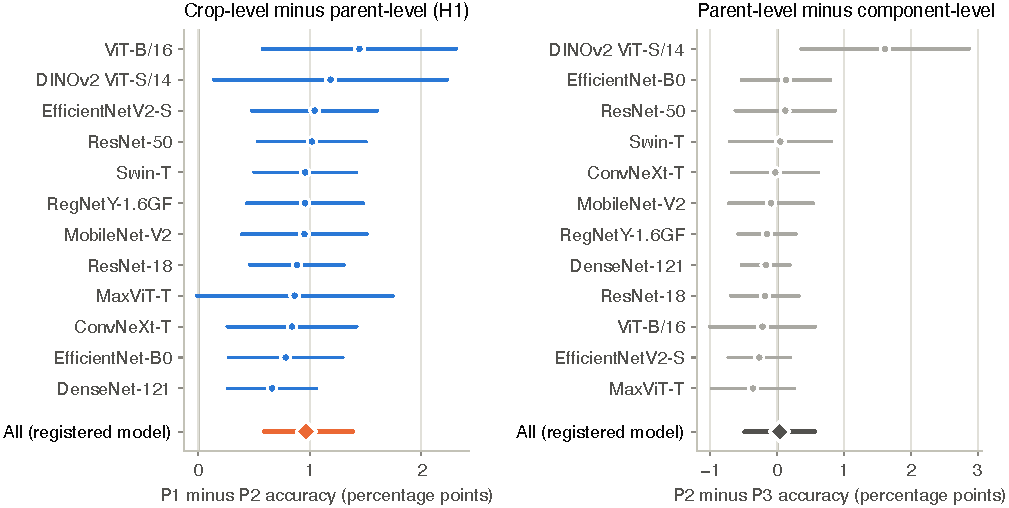
\includegraphics[width=\textwidth]{h1.pdf}
\caption{P1 $-$ P2 (left) and P2 $-$ P3 (right) per architecture (mean and 95\% $t$ interval over 20 seeds) with the
registered pooled estimates.}
\label{r:fig:h1}
\end{figure}

{\scriptsize
\setlength{\tabcolsep}{3.5pt}
\begin{longtable}{llrrrrrrrrl}
\caption{Every protocol model with its registered sensitivity analyses: Satterthwaite and Kenward--Roger degrees of freedom, two-way cluster bootstrap, and seed sign-flip test. The primary source is the bootstrap when the registered residual check fails.}\label{r:tab:sensitivity}\\
\toprule
Contrast & Model & Est. & SE & df$_S$ & $p_S$ & df$_{KR}$ & $p_{KR}$ & Bootstrap CI & Sign-flip $p$ & Primary \\
\midrule
\endfirsthead
\toprule
Contrast & Model & Est. & SE & df$_S$ & $p_S$ & df$_{KR}$ & $p_{KR}$ & Bootstrap CI & Sign-flip $p$ & Primary \\
\midrule
\endhead
\bottomrule
\endfoot
H1 accuracy & full & 0.97 & 0.17 & 38.8 & $<$0.001 & 18.8 & $<$0.001 & 0.59--1.39 & $<$0.001 & cluster\_bootstrap \\
H1 macro-F1 & full & 0.96 & 0.17 & 38.8 & $<$0.001 & 18.7 & $<$0.001 & 0.59--1.39 & $<$0.001 & cluster\_bootstrap \\
H1 balanced accuracy & full & 0.98 & 0.17 & 38.8 & $<$0.001 & 18.7 & $<$0.001 & 0.60--1.40 & $<$0.001 & cluster\_bootstrap \\
P2 $-$ P3 accuracy & full & 0.03 & 0.25 & 25.7 & 0.90 & 25.2 & 0.90 & \textminus{}0.45--0.60 & 0.88 & lmm \\
H2 CRIC accuracy & full & 12.08 & 0.40 & 8.8 & $<$0.001 & 8.8 & $<$0.001 & 11.23--12.92 & 0.002 & lmm \\
CRIC P1$'$ $-$ P2 & full & 12.11 & 0.43 & 17.5 & $<$0.001 & 10.1 & $<$0.001 & 11.21--13.05 & 0.002 & lmm \\
CRIC balanced accuracy & full & 19.64 & 0.71 & 18.0 & $<$0.001 & 7.2 & $<$0.001 & 18.00--21.34 & 0.002 & lmm \\
CRIC macro-F1 & full & 20.59 & 0.60 & 6.3 & $<$0.001 & 6.3 & $<$0.001 & 19.19--22.02 & 0.002 & lmm \\
\end{longtable}
}


\section{Consistency}

All \HonePositiveArchs\ architectures scored higher under P1 (\HoneArchMin--\HoneArchMax~pp) and \HoneArchCIPositive\ of
them individually had intervals excluding zero. At the seed level the picture is noisier but one-sided
(Figure~\ref{r:fig:seed-heatmap}). The parent-level error rate is \SipErrorRatio\ times the crop-level one. Macro-F1
(\HoneFoneEst~pp) and balanced accuracy (\HoneBaccEst~pp) moved by the same amount.

\begin{figure}[H]
\centering
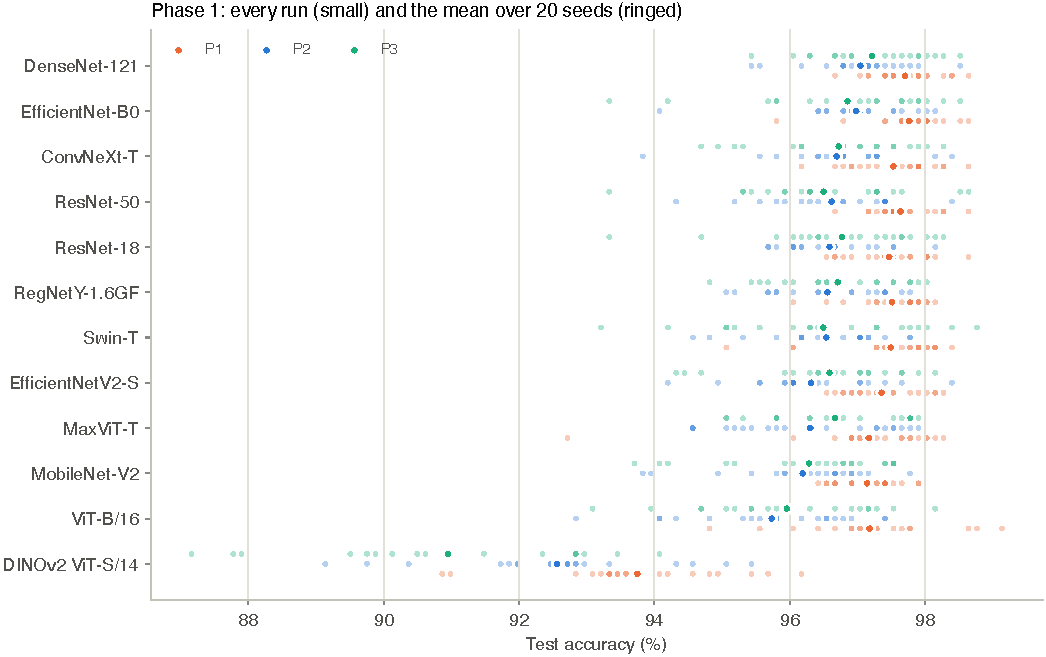
\includegraphics[width=\textwidth]{phase1_points.pdf}
\caption{Every Phase~1 run and the per-protocol mean over 20 seeds, by architecture.}
\label{r:fig:phase1-points}
\end{figure}

\begin{figure}[H]
\centering
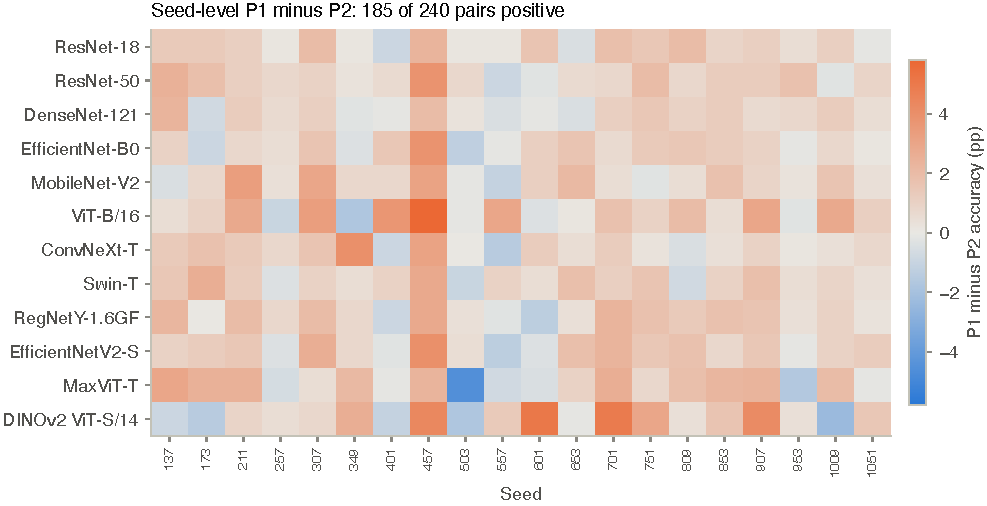
\includegraphics[width=\textwidth]{seed_heatmap.pdf}
\caption{P1 $-$ P2 accuracy for every architecture and seed (diverging scale, zero in grey).}
\label{r:fig:seed-heatmap}
\end{figure}

\begin{figure}[H]
\centering
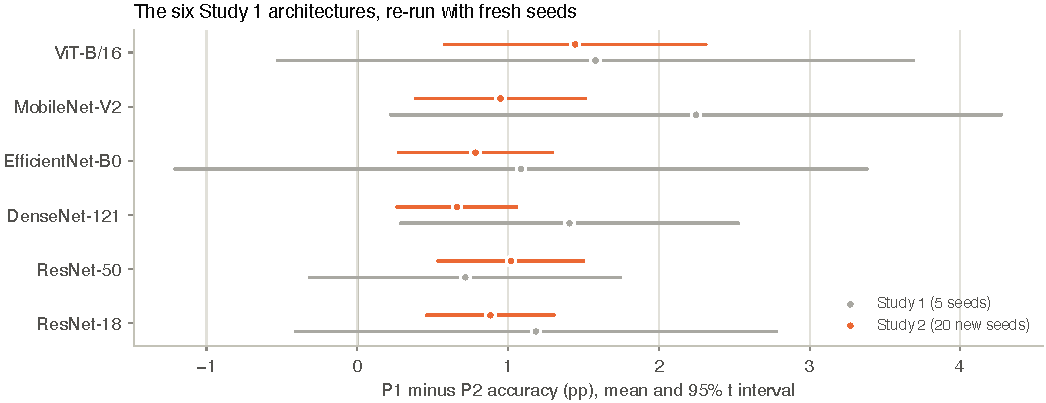
\includegraphics[width=\textwidth]{cross_study.pdf}
\caption{The six Study~1 architectures: Study~1's five-seed estimates and Study~2's twenty-seed estimates of P1 $-$ P2.
Study~2's intervals are narrower and all exclude zero.}
\label{r:fig:cross-study}
\end{figure}

\section{P2 versus P3, rankings, and the ordering gate}

Merging near-duplicate-linked parents on top of parent-level splitting changed nothing (P2 $-$ P3 \PtwoPthreeEst~pp,
\PtwoPthreeLo\ to \PtwoPthreeHi, $p=\PtwoPthreeP$). The registered P3 $\leq$ P2 $\leq$ P1 ordering passed for
\RecOrderingPassed\ of twelve architectures, as expected when two protocols are equivalent and the order between them is
decided by noise. The architecture ranking was largely preserved between P1 and P2 (Kendall $\tau=\KendallTau$,
\KendallLo--\KendallHi; \ReorderedPairs\ pairs reordered).

\section{Crop-level evidence}

Within crops that were test crops under both protocols in different seeds (\MoneCrops\ crops), accuracy was \MoneEst~pp
higher under P1 (\MoneLo--\MoneHi; M1). Within P1, a crop sharing source pixels with a training crop was more often
correct (log odds \MtwoOverlapLogOdds, $p$ \MtwoOverlapP), as was a crop with more training siblings (log odds
\MtwoSiblingsLogOdds\ per log sibling, $p=\MtwoSiblingsP$), adjusting for class and the crop's difficulty under P2 (M2).

\section{Training behaviour}

\begin{figure}[H]
\centering
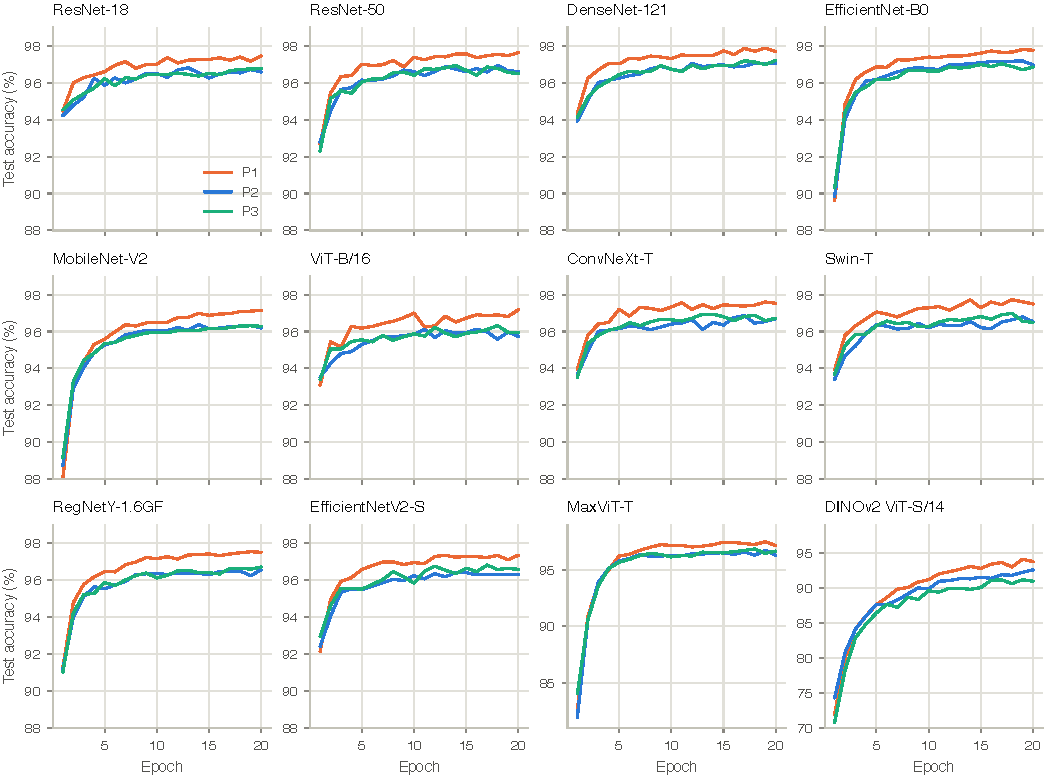
\includegraphics[width=\textwidth]{training_curves.pdf}
\caption{Mean test accuracy per epoch under P1, P2, and P3 (20 seeds each). The P1 advantage appears within the first
few epochs and persists to the final-epoch endpoint.}
\label{r:fig:training-curves}
\end{figure}

\begin{figure}[H]
\centering
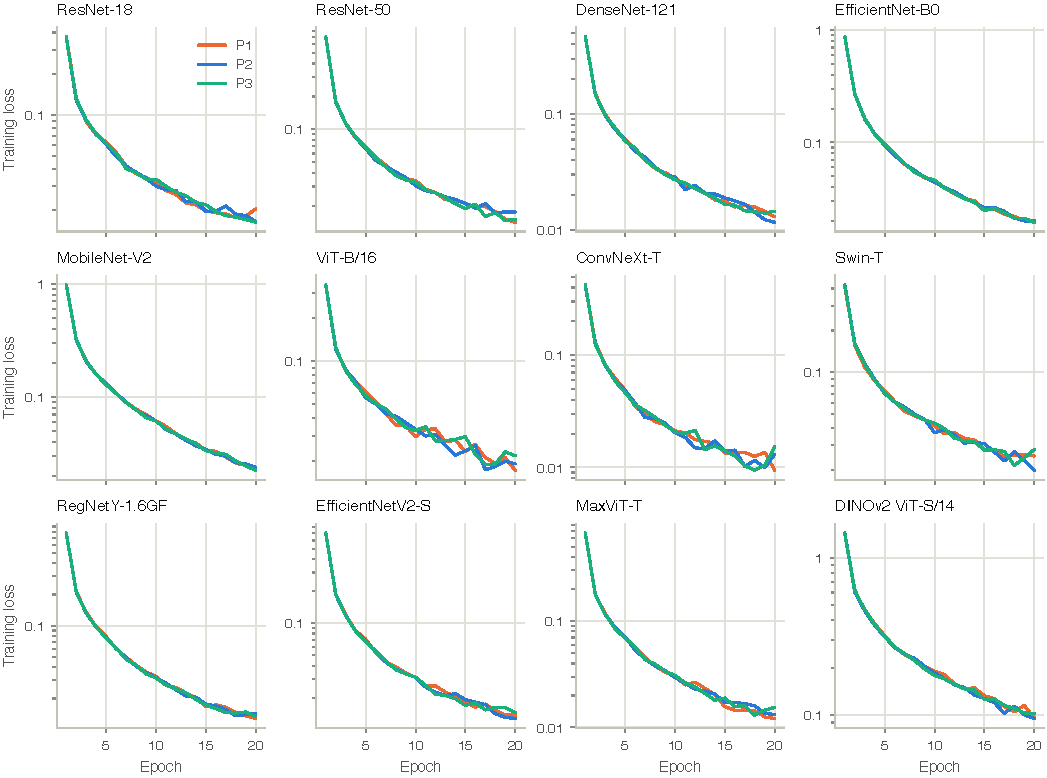
\includegraphics[width=\textwidth]{loss_curves.pdf}
\caption{Mean training loss per epoch (log scale). Training is indistinguishable across protocols; the difference is in
what the test set contains, not in how training proceeds.}
\label{r:fig:loss-curves}
\end{figure}

\section{Calibration and errors}

Pooled over runs, the 15-bin expected calibration error was \RecEceOne\% under P1, \RecEceTwo\% under P2, and
\RecEceThree\% under P3, and the negative log-likelihood \RecNllOne, \RecNllTwo, and \RecNllThree\ nats: crop-level
splits flatter calibration as well as accuracy.

\begin{figure}[H]
\centering
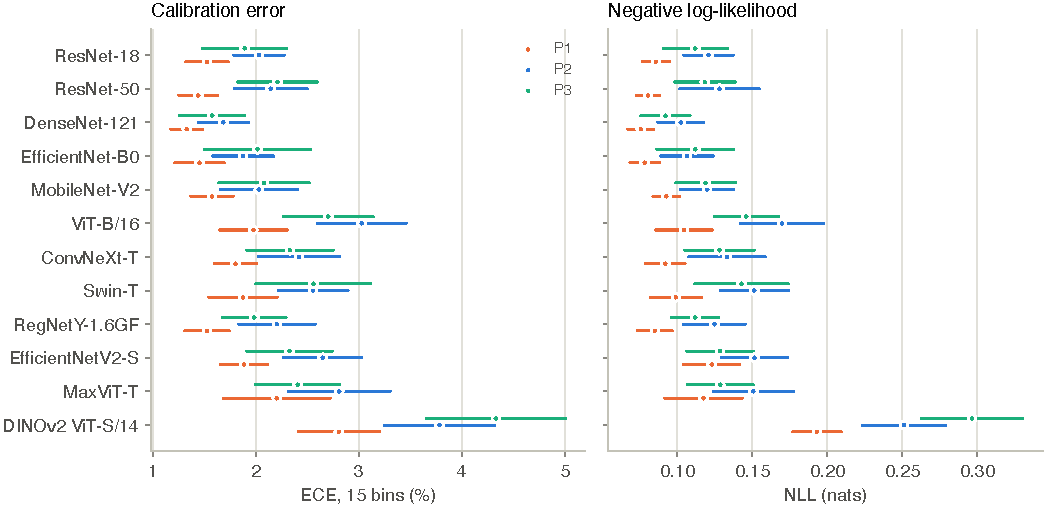
\includegraphics[width=\textwidth]{calibration.pdf}
\caption{Calibration error and negative log-likelihood by architecture and protocol (mean and 95\% $t$ interval).}
\label{r:fig:calibration}
\end{figure}

{\footnotesize
\setlength{\tabcolsep}{3.5pt}
\begin{longtable}{llrrrrr}
\caption{Phase 1 (SIPaKMeD, 20 seeds per cell): test metrics in percent (mean\,$\pm$\,SD over seeds); NLL in nats.}\label{r:tab:phase1}\\
\toprule
Architecture & Prot. & Accuracy & Macro-F1 & Balanced acc. & ECE & NLL \\
\midrule
\endfirsthead
\toprule
Architecture & Prot. & Accuracy & Macro-F1 & Balanced acc. & ECE & NLL \\
\midrule
\endhead
\bottomrule
\endfoot
ResNet-18 & P1 & 97.47\,$\pm$\,0.56 & 97.48\,$\pm$\,0.56 & 97.49\,$\pm$\,0.56 & 1.52\,$\pm$\,0.44 & 0.086 \\
 & P2 & 96.59\,$\pm$\,0.68 & 96.60\,$\pm$\,0.67 & 96.59\,$\pm$\,0.68 & 2.03\,$\pm$\,0.53 & 0.121 \\
 & P3 & 96.77\,$\pm$\,1.22 & 96.78\,$\pm$\,1.21 & 96.77\,$\pm$\,1.21 & 1.89\,$\pm$\,0.87 & 0.112 \\
ResNet-50 & P1 & 97.64\,$\pm$\,0.46 & 97.65\,$\pm$\,0.45 & 97.65\,$\pm$\,0.46 & 1.44\,$\pm$\,0.40 & 0.080 \\
 & P2 & 96.62\,$\pm$\,0.94 & 96.63\,$\pm$\,0.94 & 96.62\,$\pm$\,0.94 & 2.14\,$\pm$\,0.75 & 0.128 \\
 & P3 & 96.50\,$\pm$\,1.23 & 96.51\,$\pm$\,1.23 & 96.49\,$\pm$\,1.26 & 2.21\,$\pm$\,0.82 & 0.118 \\
DenseNet-121 & P1 & 97.70\,$\pm$\,0.51 & 97.71\,$\pm$\,0.51 & 97.72\,$\pm$\,0.51 & 1.33\,$\pm$\,0.33 & 0.076 \\
 & P2 & 97.04\,$\pm$\,0.74 & 97.05\,$\pm$\,0.74 & 97.05\,$\pm$\,0.74 & 1.68\,$\pm$\,0.52 & 0.102 \\
 & P3 & 97.22\,$\pm$\,0.83 & 97.23\,$\pm$\,0.83 & 97.21\,$\pm$\,0.83 & 1.57\,$\pm$\,0.68 & 0.092 \\
EfficientNet-B0 & P1 & 97.77\,$\pm$\,0.61 & 97.77\,$\pm$\,0.62 & 97.78\,$\pm$\,0.61 & 1.45\,$\pm$\,0.51 & 0.078 \\
 & P2 & 96.98\,$\pm$\,0.86 & 96.98\,$\pm$\,0.87 & 96.99\,$\pm$\,0.85 & 1.87\,$\pm$\,0.64 & 0.106 \\
 & P3 & 96.85\,$\pm$\,1.35 & 96.86\,$\pm$\,1.34 & 96.86\,$\pm$\,1.34 & 2.01\,$\pm$\,1.10 & 0.112 \\
MobileNet-V2 & P1 & 97.14\,$\pm$\,0.46 & 97.15\,$\pm$\,0.46 & 97.16\,$\pm$\,0.46 & 1.57\,$\pm$\,0.44 & 0.093 \\
 & P2 & 96.19\,$\pm$\,1.01 & 96.20\,$\pm$\,1.01 & 96.19\,$\pm$\,1.02 & 2.03\,$\pm$\,0.80 & 0.120 \\
 & P3 & 96.28\,$\pm$\,1.22 & 96.29\,$\pm$\,1.22 & 96.28\,$\pm$\,1.22 & 2.08\,$\pm$\,0.94 & 0.119 \\
ViT-B/16 & P1 & 97.18\,$\pm$\,1.03 & 97.19\,$\pm$\,1.02 & 97.19\,$\pm$\,1.04 & 1.97\,$\pm$\,0.70 & 0.104 \\
 & P2 & 95.73\,$\pm$\,1.21 & 95.73\,$\pm$\,1.23 & 95.74\,$\pm$\,1.21 & 3.02\,$\pm$\,0.92 & 0.170 \\
 & P3 & 95.96\,$\pm$\,1.30 & 95.96\,$\pm$\,1.31 & 95.97\,$\pm$\,1.30 & 2.70\,$\pm$\,0.93 & 0.146 \\
ConvNeXt-T & P1 & 97.53\,$\pm$\,0.64 & 97.54\,$\pm$\,0.63 & 97.54\,$\pm$\,0.64 & 1.80\,$\pm$\,0.43 & 0.092 \\
 & P2 & 96.69\,$\pm$\,0.95 & 96.70\,$\pm$\,0.94 & 96.69\,$\pm$\,0.95 & 2.42\,$\pm$\,0.84 & 0.133 \\
 & P3 & 96.72\,$\pm$\,1.06 & 96.72\,$\pm$\,1.07 & 96.73\,$\pm$\,1.05 & 2.33\,$\pm$\,0.89 & 0.128 \\
Swin-T & P1 & 97.49\,$\pm$\,0.84 & 97.50\,$\pm$\,0.84 & 97.51\,$\pm$\,0.84 & 1.87\,$\pm$\,0.71 & 0.099 \\
 & P2 & 96.54\,$\pm$\,0.89 & 96.55\,$\pm$\,0.88 & 96.55\,$\pm$\,0.88 & 2.55\,$\pm$\,0.72 & 0.151 \\
 & P3 & 96.49\,$\pm$\,1.46 & 96.50\,$\pm$\,1.47 & 96.50\,$\pm$\,1.46 & 2.56\,$\pm$\,1.19 & 0.143 \\
RegNetY-1.6GF & P1 & 97.51\,$\pm$\,0.54 & 97.52\,$\pm$\,0.54 & 97.53\,$\pm$\,0.54 & 1.52\,$\pm$\,0.47 & 0.085 \\
 & P2 & 96.56\,$\pm$\,0.83 & 96.57\,$\pm$\,0.84 & 96.56\,$\pm$\,0.83 & 2.20\,$\pm$\,0.79 & 0.125 \\
 & P3 & 96.71\,$\pm$\,0.93 & 96.72\,$\pm$\,0.94 & 96.71\,$\pm$\,0.93 & 1.98\,$\pm$\,0.66 & 0.112 \\
EfficientNetV2-S & P1 & 97.36\,$\pm$\,0.54 & 97.37\,$\pm$\,0.54 & 97.37\,$\pm$\,0.53 & 1.88\,$\pm$\,0.49 & 0.123 \\
 & P2 & 96.31\,$\pm$\,0.95 & 96.32\,$\pm$\,0.96 & 96.32\,$\pm$\,0.95 & 2.65\,$\pm$\,0.81 & 0.151 \\
 & P3 & 96.59\,$\pm$\,1.09 & 96.59\,$\pm$\,1.09 & 96.59\,$\pm$\,1.09 & 2.32\,$\pm$\,0.88 & 0.128 \\
MaxViT-T & P1 & 97.17\,$\pm$\,1.19 & 97.17\,$\pm$\,1.20 & 97.19\,$\pm$\,1.18 & 2.20\,$\pm$\,1.11 & 0.117 \\
 & P2 & 96.30\,$\pm$\,1.21 & 96.31\,$\pm$\,1.20 & 96.31\,$\pm$\,1.21 & 2.81\,$\pm$\,1.06 & 0.151 \\
 & P3 & 96.67\,$\pm$\,0.97 & 96.67\,$\pm$\,0.98 & 96.68\,$\pm$\,0.97 & 2.40\,$\pm$\,0.87 & 0.129 \\
DINOv2 ViT-S/14 & P1 & 93.75\,$\pm$\,1.34 & 93.78\,$\pm$\,1.33 & 93.79\,$\pm$\,1.33 & 2.80\,$\pm$\,0.85 & 0.193 \\
 & P2 & 92.56\,$\pm$\,1.60 & 92.61\,$\pm$\,1.55 & 92.61\,$\pm$\,1.60 & 3.78\,$\pm$\,1.15 & 0.251 \\
 & P3 & 90.95\,$\pm$\,1.95 & 90.99\,$\pm$\,1.92 & 90.99\,$\pm$\,1.95 & 4.33\,$\pm$\,1.45 & 0.297 \\
\end{longtable}
}


\chapter{H2: the CRIC inflation is an order of magnitude larger}
\label{r:ch:h2}

CRIC accuracy fell from \CricPOneAcc\% under crop-level splitting to \CricPTwoAcc\% under slide-level splitting:
H2 $=$ \HtwoEst~pp (\HtwoLo--\HtwoHi; Holm $p$ \HtwoPholm). The error rate rose \CricErrorRatio-fold. Because the classes
are imbalanced, balanced accuracy fell further, from \CricPOneBacc\% to \CricPTwoBacc\% (\CricBaccEst~pp), and macro-F1 by
\CricFoneEst~pp. The size-matched P1-prime gave the same inflation (\CricPrimeEst~pp), so it is not a training-size
effect.

\begin{figure}[H]
\centering
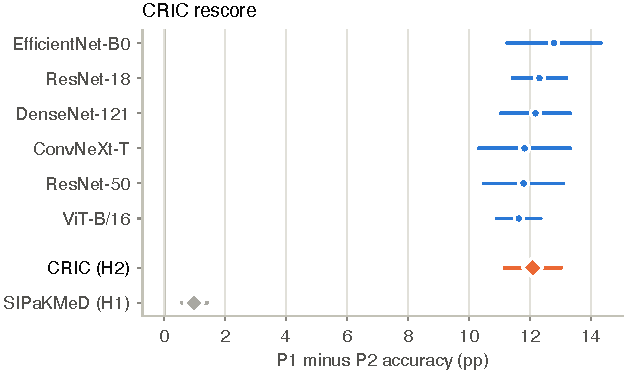
\includegraphics[width=0.85\textwidth]{cric.pdf}
\caption{CRIC P1 $-$ P2 per architecture, the registered estimate, and the SIPaKMeD estimate for scale.}
\label{r:fig:cric}
\end{figure}

The loss is concentrated in the abnormal classes (Figure~\ref{r:fig:cric-recall}). Recall for ASC-H, LSIL, and HSIL falls
by tens of points when slides are held out, while the majority NILM class barely moves; the crop-level split had been
rewarding the recognition of slides whose abnormal cells were already seen.

\begin{figure}[H]
\centering
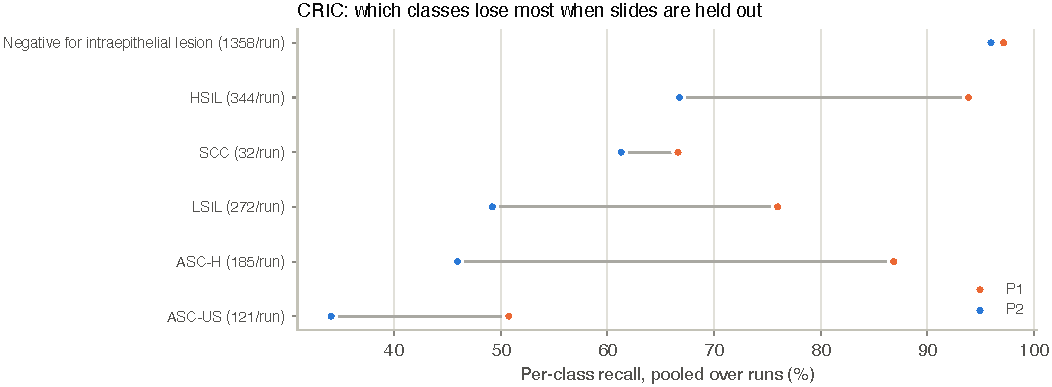
\includegraphics[width=\textwidth]{cric_recall.pdf}
\caption{CRIC per-class recall under P1 and P2, pooled over all runs, with the mean number of test cells per class.}
\label{r:fig:cric-recall}
\end{figure}

\begin{figure}[H]
\centering
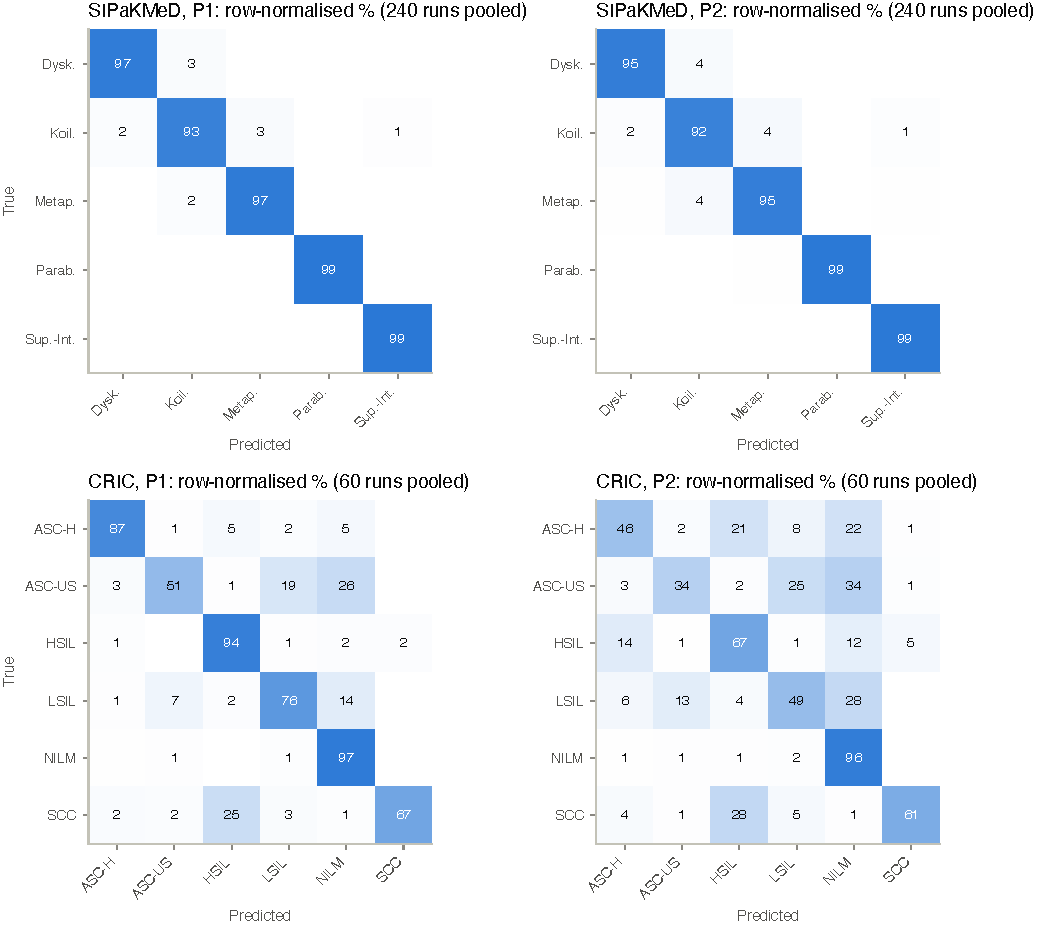
\includegraphics[width=\textwidth]{confusion.pdf}
\caption{Row-normalised confusion matrices pooled over runs. SIPaKMeD errors barely change between protocols; CRIC's
abnormal classes collapse toward NILM and toward each other under slide-level splitting.}
\label{r:fig:confusion}
\end{figure}

{\footnotesize
\setlength{\tabcolsep}{3.5pt}
\begin{longtable}{llrrrrr}
\caption{CRIC (10 seeds per cell): test metrics in percent (mean\,$\pm$\,SD).}\label{r:tab:cric}\\
\toprule
Architecture & Prot. & Accuracy & Macro-F1 & Balanced acc. & ECE & NLL \\
\midrule
\endfirsthead
\toprule
Architecture & Prot. & Accuracy & Macro-F1 & Balanced acc. & ECE & NLL \\
\midrule
\endhead
\bottomrule
\endfoot
ResNet-18 & P1 & 89.91\,$\pm$\,0.43 & 79.09\,$\pm$\,1.31 & 77.60\,$\pm$\,2.07 & 5.50\,$\pm$\,0.40 & 0.383 \\
 & P1-prime & 89.92\,$\pm$\,0.68 & 78.94\,$\pm$\,1.43 & 77.42\,$\pm$\,2.25 & 5.48\,$\pm$\,0.67 & 0.387 \\
 & P2 & 77.62\,$\pm$\,1.14 & 57.25\,$\pm$\,1.45 & 56.79\,$\pm$\,2.63 & 14.98\,$\pm$\,1.11 & 1.014 \\
ResNet-50 & P1 & 90.54\,$\pm$\,0.48 & 80.48\,$\pm$\,1.63 & 79.42\,$\pm$\,2.41 & 5.85\,$\pm$\,0.33 & 0.388 \\
 & P1-prime & 90.85\,$\pm$\,0.62 & 81.01\,$\pm$\,1.66 & 79.85\,$\pm$\,2.02 & 5.41\,$\pm$\,0.45 & 0.371 \\
 & P2 & 78.76\,$\pm$\,1.80 & 60.48\,$\pm$\,3.30 & 60.34\,$\pm$\,2.84 & 14.97\,$\pm$\,1.82 & 0.995 \\
DenseNet-121 & P1 & 90.40\,$\pm$\,0.74 & 79.66\,$\pm$\,1.93 & 77.97\,$\pm$\,2.71 & 5.42\,$\pm$\,0.68 & 0.374 \\
 & P1-prime & 90.71\,$\pm$\,0.48 & 80.22\,$\pm$\,1.41 & 78.32\,$\pm$\,1.76 & 5.36\,$\pm$\,0.46 & 0.365 \\
 & P2 & 78.23\,$\pm$\,1.50 & 59.08\,$\pm$\,2.36 & 58.82\,$\pm$\,2.77 & 14.95\,$\pm$\,1.28 & 1.017 \\
EfficientNet-B0 & P1 & 90.88\,$\pm$\,0.53 & 80.74\,$\pm$\,0.99 & 79.78\,$\pm$\,1.46 & 5.33\,$\pm$\,0.43 & 0.370 \\
 & P1-prime & 90.95\,$\pm$\,0.60 & 80.95\,$\pm$\,1.05 & 80.83\,$\pm$\,1.64 & 5.21\,$\pm$\,0.54 & 0.363 \\
 & P2 & 78.10\,$\pm$\,2.15 & 58.73\,$\pm$\,2.78 & 59.86\,$\pm$\,2.19 & 14.90\,$\pm$\,1.74 & 1.021 \\
ViT-B/16 & P1 & 89.83\,$\pm$\,0.63 & 78.01\,$\pm$\,2.30 & 76.37\,$\pm$\,3.22 & 6.54\,$\pm$\,0.95 & 0.436 \\
 & P1-prime & 89.54\,$\pm$\,0.70 & 78.28\,$\pm$\,1.81 & 76.45\,$\pm$\,2.95 & 6.55\,$\pm$\,0.68 & 0.429 \\
 & P2 & 78.20\,$\pm$\,1.13 & 59.54\,$\pm$\,1.47 & 57.62\,$\pm$\,2.28 & 16.14\,$\pm$\,1.29 & 1.054 \\
ConvNeXt-T & P1 & 91.29\,$\pm$\,0.63 & 81.80\,$\pm$\,1.57 & 80.03\,$\pm$\,2.69 & 5.91\,$\pm$\,0.58 & 0.392 \\
 & P1-prime & 91.10\,$\pm$\,0.40 & 80.73\,$\pm$\,1.97 & 78.85\,$\pm$\,2.17 & 6.02\,$\pm$\,0.53 & 0.392 \\
 & P2 & 79.48\,$\pm$\,1.78 & 61.15\,$\pm$\,3.27 & 59.90\,$\pm$\,3.99 & 15.82\,$\pm$\,1.76 & 1.082 \\
\end{longtable}
}


\chapter{H3: the inflation is leakage, not training diversity}
\label{r:ch:h3}

With crop count, field count, and allocation rule held equal, adding the test fields' sibling crops to training raised
accuracy on the common test set by \HthreeEst~pp (\HthreeLo--\HthreeHi; Holm $p=\HthreePholm$). Every architecture showed
it at both diversity levels (Figure~\ref{r:fig:factorial-cells}). Increasing the number of distinct training fields from
504 to 720 without leakage did nothing (\DivEst~pp, \DivLo\ to \DivHi), and the leak effect did not depend on diversity
(interaction \InteractionEst~pp, $p=\InteractionP$). The registered approximate decomposition assigns the Phase~1 gap
entirely to leakage (diversity component \DecompDiv~pp).

\begin{figure}[H]
\centering
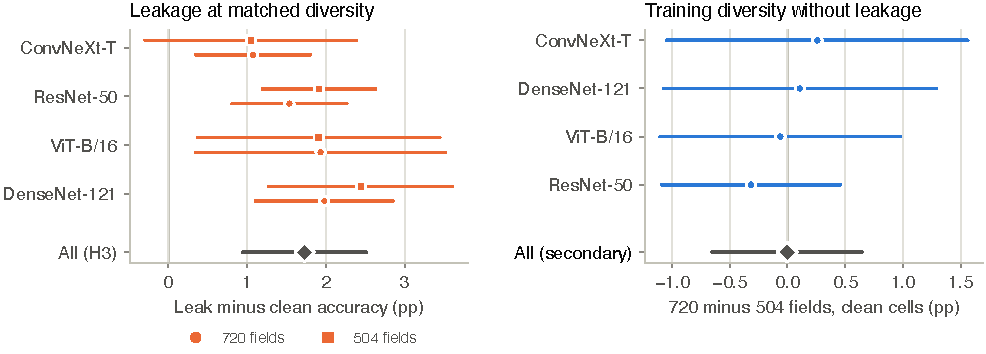
\includegraphics[width=\textwidth]{factorial.pdf}
\caption{Left: leak minus clean accuracy per architecture and diversity level, and the H3 estimate. Right: high minus
low diversity within clean cells.}
\label{r:fig:factorial}
\end{figure}

\begin{figure}[H]
\centering
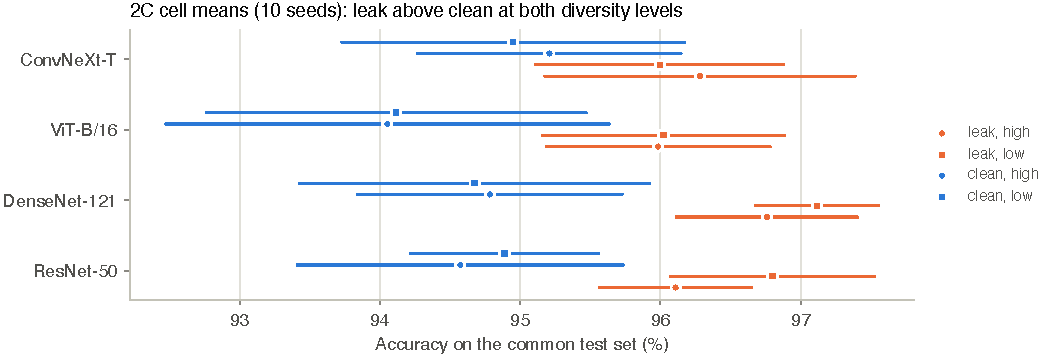
\includegraphics[width=\textwidth]{factorial_cells.pdf}
\caption{All four 2C cell means per architecture (10 seeds each).}
\label{r:fig:factorial-cells}
\end{figure}

The diversity manipulation did change what the training sets contain. In the embedding space of a retrained parent-probe
encoder (which identified held-out fields at \RecEncoderAcc\% against \RecEncoderChance\% chance), the mean distance between
field centroids was \RecDivCleanHigh\ for 720-field and \RecDivCleanLow\ for 504-field clean training sets, and
\RecDivPOne\ (P1, \RecDivParentsPOne\ fields) against \RecDivPTwo\ (P2, \RecDivParentsPTwo\ fields) for the natural splits.
More diverse training sets were measurably more diverse; that diversity simply did not improve accuracy.

\chapter{H4: background transplants do not isolate the route}
\label{r:ch:h4}

\begin{figure}[H]
\centering
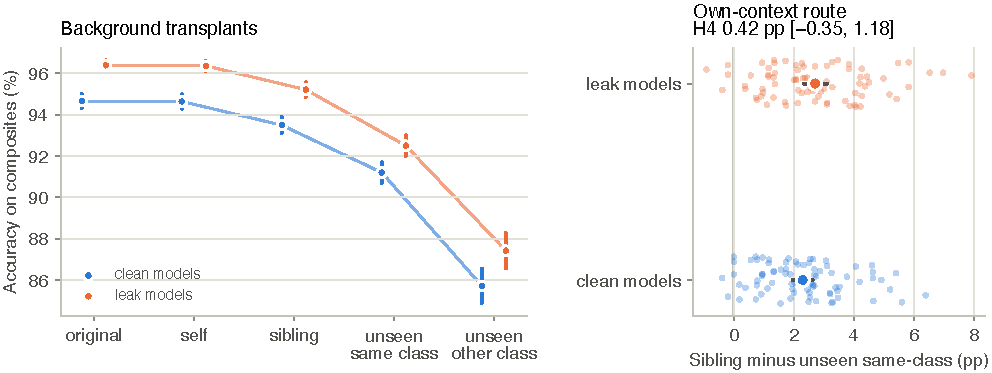
\includegraphics[width=\textwidth]{transplant.pdf}
\caption{Left: accuracy of leak and clean models on composites of the common test set. Right: the per-run own-context
route and the registered H4 contrast.}
\label{r:fig:transplant}
\end{figure}

Compositing a cell onto its own inpainted background cost nothing, so seam and inpainting artifacts were negligible.
Leak models were \LeakOriginalEst~pp more accurate than clean models on unmodified cells and kept most of that advantage
when the background was replaced: \TransplantLeakSibling~pp on sibling backgrounds, \TransplantLeakUnseen~pp on backgrounds
from unseen fields of the same class, and \TransplantLeakOther~pp on other-class backgrounds. H4, the leak-minus-clean
difference of the own-context route, was \HfourEst~pp (\HfourLo\ to \HfourHi; Holm $p=\HfourPholm$): not supported. Its
point estimate would assign \RouteShare\% of the inflation to the background.

Two observations qualify the design. Sibling backgrounds helped even clean models, which had never seen those fields, by
\TransplantCleanHarmony~pp, presumably because a background from the cell's own field matches its stain; that effect is
common to both arms but inflates the variance of the contrast. And backgrounds do carry class information: an other-class
background moved \DonorShiftEst~pp of probability toward its class (\DonorShiftLo--\DonorShiftHi, secondary). Restricting H4
to recipients whose background covers at least 30\% of the crop gave \HfourBgEst~pp (\HfourBgLo\ to \HfourBgHi).

\begin{figure}[H]
\centering
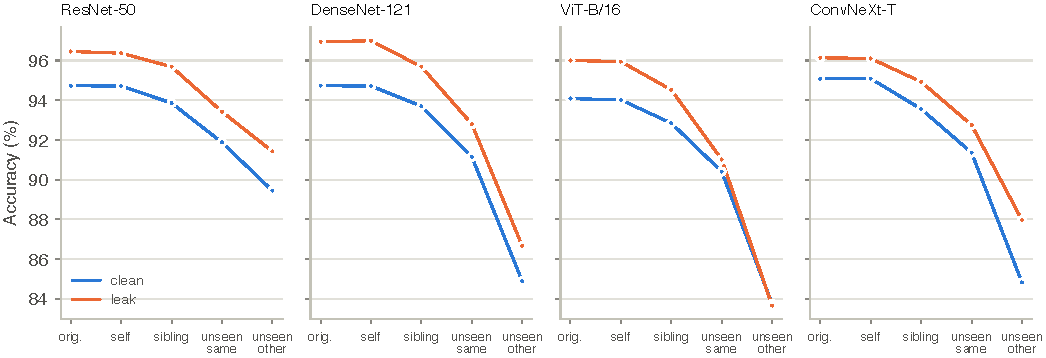
\includegraphics[width=\textwidth]{transplant_arch.pdf}
\caption{Transplant-condition accuracy of leak and clean models per architecture.}
\label{r:fig:transplant-arch}
\end{figure}

{\scriptsize
\setlength{\tabcolsep}{3.5pt}
\begin{longtable}{llrrrrrr}
\caption{2C/2B (10 seeds per cell): accuracy on the common test set and on each background-transplant condition (percent), and the donor-class probability shift (pp).}\label{r:tab:factorial}\\
\toprule
Architecture & Cell & Original & Self & Sibling & Unseen same & Unseen other & Shift \\
\midrule
\endfirsthead
\toprule
Architecture & Cell & Original & Self & Sibling & Unseen same & Unseen other & Shift \\
\midrule
\endhead
\bottomrule
\endfoot
ResNet-50 & leak\_high & 96.11\,$\pm$\,0.76 & 95.96\,$\pm$\,0.77 & 95.29\,$\pm$\,0.89 & 92.61\,$\pm$\,1.41 & 90.89\,$\pm$\,1.24 & 1.19 \\
 & clean\_high & 94.57\,$\pm$\,1.63 & 94.50\,$\pm$\,1.78 & 93.43\,$\pm$\,2.06 & 91.73\,$\pm$\,1.94 & 89.03\,$\pm$\,2.49 & 1.35 \\
 & leak\_low & 96.80\,$\pm$\,1.02 & 96.78\,$\pm$\,1.03 & 96.08\,$\pm$\,1.03 & 94.23\,$\pm$\,1.40 & 91.95\,$\pm$\,1.50 & 1.33 \\
 & clean\_low & 94.89\,$\pm$\,0.94 & 94.93\,$\pm$\,0.83 & 94.28\,$\pm$\,0.84 & 92.02\,$\pm$\,1.20 & 89.85\,$\pm$\,1.16 & 1.22 \\
DenseNet-121 & leak\_high & 96.76\,$\pm$\,0.91 & 96.89\,$\pm$\,0.77 & 95.67\,$\pm$\,0.60 & 92.80\,$\pm$\,1.51 & 86.79\,$\pm$\,1.96 & 4.15 \\
 & clean\_high & 94.78\,$\pm$\,1.32 & 94.78\,$\pm$\,1.26 & 93.72\,$\pm$\,1.20 & 90.97\,$\pm$\,1.99 & 84.58\,$\pm$\,2.57 & 4.50 \\
 & leak\_low & 97.12\,$\pm$\,0.62 & 97.10\,$\pm$\,0.65 & 95.70\,$\pm$\,1.28 & 92.80\,$\pm$\,2.21 & 86.52\,$\pm$\,2.90 & 4.36 \\
 & clean\_low & 94.67\,$\pm$\,1.75 & 94.65\,$\pm$\,1.83 & 93.68\,$\pm$\,1.63 & 91.33\,$\pm$\,2.28 & 85.19\,$\pm$\,3.46 & 4.08 \\
ViT-B/16 & leak\_high & 95.98\,$\pm$\,1.12 & 95.93\,$\pm$\,1.22 & 94.55\,$\pm$\,2.45 & 90.44\,$\pm$\,2.89 & 84.05\,$\pm$\,3.05 & 3.66 \\
 & clean\_high & 94.05\,$\pm$\,2.21 & 94.05\,$\pm$\,2.18 & 92.82\,$\pm$\,2.27 & 90.73\,$\pm$\,2.43 & 84.62\,$\pm$\,4.51 & 3.36 \\
 & leak\_low & 96.02\,$\pm$\,1.21 & 95.96\,$\pm$\,1.25 & 94.49\,$\pm$\,1.36 & 91.58\,$\pm$\,2.25 & 83.26\,$\pm$\,3.68 & 4.39 \\
 & clean\_low & 94.11\,$\pm$\,1.90 & 93.98\,$\pm$\,1.97 & 92.86\,$\pm$\,2.61 & 90.07\,$\pm$\,3.20 & 82.87\,$\pm$\,3.39 & 3.93 \\
ConvNeXt-T & leak\_high & 96.28\,$\pm$\,1.55 & 96.25\,$\pm$\,1.63 & 95.01\,$\pm$\,1.34 & 92.69\,$\pm$\,1.81 & 87.79\,$\pm$\,3.44 & 2.71 \\
 & clean\_high & 95.21\,$\pm$\,1.31 & 95.19\,$\pm$\,1.22 & 93.89\,$\pm$\,1.32 & 91.83\,$\pm$\,2.40 & 85.63\,$\pm$\,2.63 & 3.03 \\
 & leak\_low & 96.00\,$\pm$\,1.24 & 95.96\,$\pm$\,1.17 & 94.84\,$\pm$\,2.61 & 92.81\,$\pm$\,3.30 & 88.13\,$\pm$\,3.33 & 2.81 \\
 & clean\_low & 94.95\,$\pm$\,1.71 & 94.99\,$\pm$\,1.66 & 93.22\,$\pm$\,2.09 & 90.89\,$\pm$\,2.82 & 84.00\,$\pm$\,4.02 & 3.40 \\
\end{longtable}
}


\chapter{H5: gradient reversal was evaded}
\label{r:ch:h5}

\begin{figure}[H]
\centering
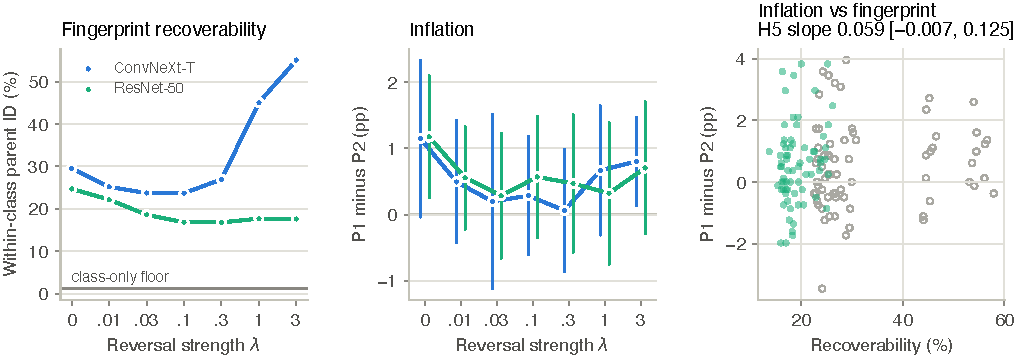
\includegraphics[width=\textwidth]{grl.pdf}
\caption{The gradient-reversal sweep: probe recoverability, the P1 $-$ P2 gap, and their relation (ConvNeXt-T, which
failed its manipulation check, hollow).}
\label{r:fig:grl}
\end{figure}

For ConvNeXt-T the adversary was evaded: as the reversal strength grew, an independent linear probe identified the field
\emph{better} (\GrlConvRzero\% at $\lambda=0$, \GrlConvRstar\% at $\lambda=3$), while the adversary's own training accuracy
fell toward chance (Figure~\ref{r:fig:grl-full}). The encoder learned features its two-layer adversary could not read but a
standardised linear probe could, the failure mode described for adversarial removal in language
models~\citep{elazar2018adversarial}. ConvNeXt-T therefore failed the registered manipulation check and was excluded. For
ResNet-50, recoverability fell from \GrlResRzero\% to \GrlResRstar\% and the mean gap fell from \GrlResGapZero~pp to
between \GrlResGapMin\ and \GrlResGapMax~pp at every $\lambda>0$, with P2 accuracy within 1~pp. The registered slope was
positive but not significant (\HfiveEst\ pp per pp, \HfiveLo\ to \HfiveHi; Holm $p=\HfivePholm$). Amendment~8's linear
adversary later showed the ResNet-50 gap does not fall when recoverability is suppressed on fresh seeds (Part~VI), so this
drop was most likely noise.

\begin{figure}[H]
\centering
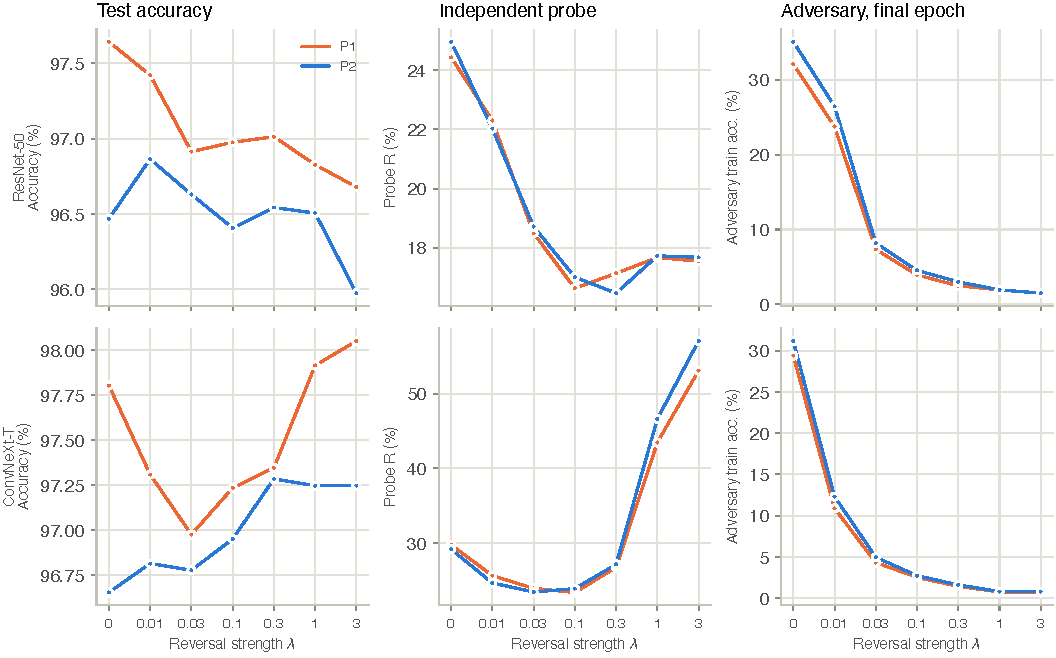
\includegraphics[width=\textwidth]{grl_full.pdf}
\caption{The full 2A sweep per architecture: test accuracy, independent-probe recoverability, and the adversary's own
within-class training accuracy at the final epoch.}
\label{r:fig:grl-full}
\end{figure}

{\footnotesize
\setlength{\tabcolsep}{3.5pt}
\begin{longtable}{lrrrrrr}
\caption{2A gradient-reversal sweep (10 seeds): accuracy (percent), mean gap (pp), and within-class parent recoverability $R$ of the frozen features (percent; sklearn probe).}\label{r:tab:grl}\\
\toprule
Architecture & $\lambda$ & P1 acc. & P2 acc. & Gap & $R$ (P1) & $R$ (P2) \\
\midrule
\endfirsthead
\toprule
Architecture & $\lambda$ & P1 acc. & P2 acc. & Gap & $R$ (P1) & $R$ (P2) \\
\midrule
\endhead
\bottomrule
\endfoot
ResNet-50 & 0 & 97.64\,$\pm$\,0.46 & 96.47\,$\pm$\,1.15 & 1.17 & 24.4\,$\pm$\,1.2 & 25.0\,$\pm$\,1.3 \\
 & 0.01 & 97.42\,$\pm$\,0.56 & 96.86\,$\pm$\,0.71 & 0.56 & 22.3\,$\pm$\,1.1 & 22.0\,$\pm$\,2.0 \\
 & 0.03 & 96.91\,$\pm$\,0.82 & 96.63\,$\pm$\,0.84 & 0.28 & 18.5\,$\pm$\,1.7 & 18.7\,$\pm$\,1.5 \\
 & 0.1 & 96.98\,$\pm$\,0.38 & 96.41\,$\pm$\,1.00 & 0.57 & 16.6\,$\pm$\,1.1 & 17.0\,$\pm$\,1.6 \\
 & 0.3 & 97.01\,$\pm$\,0.78 & 96.54\,$\pm$\,0.93 & 0.47 & 17.1\,$\pm$\,2.0 & 16.5\,$\pm$\,1.0 \\
 & 1 & 96.83\,$\pm$\,0.76 & 96.51\,$\pm$\,1.00 & 0.32 & 17.7\,$\pm$\,1.5 & 17.7\,$\pm$\,1.7 \\
 & 3 & 96.68\,$\pm$\,0.73 & 95.98\,$\pm$\,1.22 & 0.70 & 17.5\,$\pm$\,1.8 & 17.7\,$\pm$\,1.5 \\
ConvNeXt-T & 0 & 97.80\,$\pm$\,0.55 & 96.65\,$\pm$\,1.31 & 1.15 & 29.8\,$\pm$\,1.2 & 29.2\,$\pm$\,1.5 \\
 & 0.01 & 97.31\,$\pm$\,0.95 & 96.81\,$\pm$\,0.73 & 0.49 & 25.7\,$\pm$\,1.3 & 24.7\,$\pm$\,1.5 \\
 & 0.03 & 96.98\,$\pm$\,1.00 & 96.78\,$\pm$\,1.30 & 0.20 & 24.0\,$\pm$\,1.4 & 23.5\,$\pm$\,1.4 \\
 & 0.1 & 97.23\,$\pm$\,0.78 & 96.95\,$\pm$\,0.81 & 0.28 & 23.4\,$\pm$\,0.9 & 23.9\,$\pm$\,1.1 \\
 & 0.3 & 97.35\,$\pm$\,1.01 & 97.28\,$\pm$\,1.05 & 0.06 & 26.8\,$\pm$\,1.5 & 27.2\,$\pm$\,1.9 \\
 & 1 & 97.91\,$\pm$\,0.68 & 97.25\,$\pm$\,0.82 & 0.67 & 43.5\,$\pm$\,1.0 & 46.6\,$\pm$\,1.4 \\
 & 3 & 98.05\,$\pm$\,0.47 & 97.25\,$\pm$\,0.65 & 0.80 & 53.1\,$\pm$\,2.0 & 57.0\,$\pm$\,2.1 \\
\end{longtable}
}


\chapter{What Study 2 established}
\label{r:ch:s2-established}

\begin{workedbox}{Study 2 in four sentences}
Crop-level splitting inflates accuracy, by \HoneEst~pp on SIPaKMeD across twelve architectures and by \HtwoEst~pp on CRIC.
The inflation is leakage: at matched size and diversity, the test fields' siblings alone add \HthreeEst~pp, and diversity
alone adds nothing. The size of the inflation follows the dataset's structure, as the closed forms predict. How models
use the leak was not settled: the background route was small and uncertain, and the adversary was evaded.
\end{workedbox}

\part{Amendment 8: Where the Leaked Signal Lives}

\chapter{Why a follow-up, and what was known}
\label{r:ch:a8-why}

Study~2 established \emph{that} crop-level splitting inflates accuracy and that the inflation is leakage, but neither
registered mechanism test isolated \emph{how} models use it. Two observations pointed the way. Leak models kept most of
their advantage on backgrounds transplanted from unseen fields, which suggested a carrier inside the cell region rather
than in the background. And the ConvNeXt-T adversary had been evaded, so the gradient-reversal arm had only one usable
architecture.

Amendment~8 (\artifact{PREREGISTRATION_STUDY2_AMENDMENT8.md}, commit \texttt{\FollowupCommit}, \FollowupTime) registered
eight new hypotheses after the Study~2 analysis and before any follow-up model was trained or any follow-up analysis was
run on existing outputs. It states what was known and what was not: every registered Study~2 output was known, including
transplant condition means and gradient-reversal sweep means; no per-cell CRIC result by slide composition, no ablated
image evaluation, no erased-feature evaluation, no Grad-CAM map, and no model trained with masked backgrounds, colour
augmentation, stain normalisation, or the linear adversary had been seen. F1--F8 form their own Holm family, separate from
H1--H5, whose verdicts the amendment does not touch.

\begin{figure}[H]
\centering
\begin{adjustbox}{max width=\textwidth}
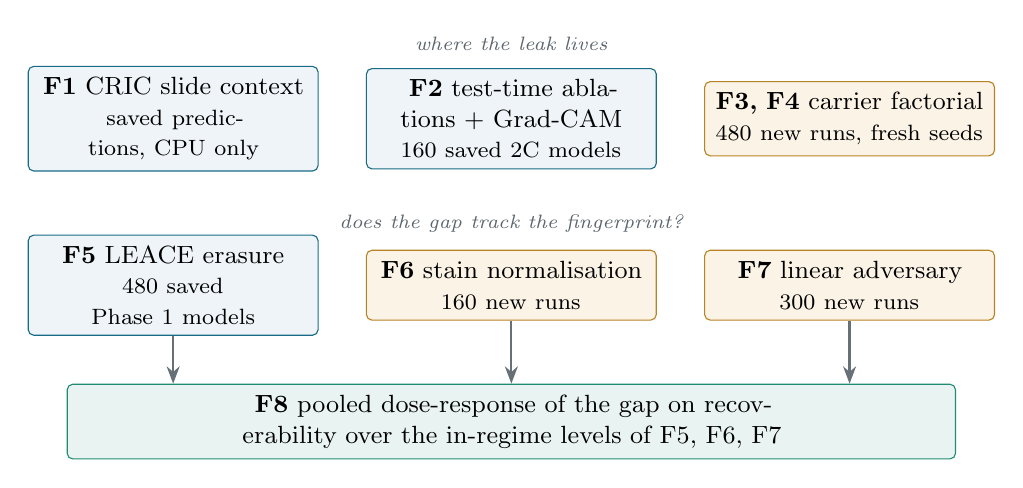
\begin{tikzpicture}[node distance=4mm and 6mm]
\node[box=34mm] (cric) {\textbf{F1} CRIC slide context\\\footnotesize saved predictions, CPU only};
\node[box=34mm, right=of cric] (abl) {\textbf{F2} test-time ablations + Grad-CAM\\\footnotesize 160 saved 2C models};
\node[gold=34mm, right=of abl] (car) {\textbf{F3, F4} carrier factorial\\\footnotesize 480 new runs, fresh seeds};
\node[box=34mm, below=8mm of cric] (leace) {\textbf{F5} LEACE erasure\\\footnotesize 480 saved Phase 1 models};
\node[gold=34mm, right=of leace] (norm) {\textbf{F6} stain normalisation\\\footnotesize 160 new runs};
\node[gold=34mm, right=of norm] (lin) {\textbf{F7} linear adversary\\\footnotesize 300 new runs};
\node[done=110mm, below=8mm of norm] (pool) {\textbf{F8} pooled dose-response of the gap on recoverability over the in-regime levels of F5, F6, F7};
\draw[flow] (leace.south) -- (leace.south |- pool.north);
\draw[flow] (norm.south) -- (pool.north);
\draw[flow] (lin.south) -- (lin.south |- pool.north);
\node[note, above=1mm of abl] {where the leak lives};
\node[note, above=1mm of norm] {does the gap track the fingerprint?};
\end{tikzpicture}
\end{adjustbox}
\caption{The eight Amendment~8 hypotheses. Blue arms reuse saved Study~2 artifacts (no retraining); gold arms train new
models on seeds no earlier arm used; F8 pools the three dose-response arms.}
\label{r:fig:followup-arms}
\end{figure}


\chapter{The eight follow-up designs}
\label{r:ch:a8-designs}

\section{F1: slide context in CRIC}

CRIC slide images contain cells of several classes (83\% of slides have more than one), so a test cell's training
siblings can carry a different label. For every cell, the \emph{context class} is the majority class of the other cells
of its slide (cells whose slide has no other cell, or a tied majority, are excluded). A \emph{discordant} cell's class
differs from its context class. If crop-level models apply a slide-level label prior, discordant cells should receive more
probability on the context class when their slide was in training (P1) than when it was not (P2). F1 is that within-cell
difference over the 120 saved CRIC P1 and P2 runs, with a percentile cluster bootstrap over slides (10,000 replicates).

\begin{figure}[H]
\centering
\begin{adjustbox}{max width=\textwidth}
\begin{tikzpicture}[node distance=4mm and 6mm, cell/.style={circle,draw=CytoInk!60,minimum size=5mm,inner sep=0pt,font=\scriptsize}]
\node[draw=CytoBlue, rounded corners, minimum width=52mm, minimum height=26mm, label={[font=\small]above:One CRIC slide image}] (slide) {};
\node[cell, fill=SerBlue!35] at ($(slide.center)+(-18mm,6mm)$) {N};
\node[cell, fill=SerBlue!35] at ($(slide.center)+(-8mm,7mm)$) {N};
\node[cell, fill=SerBlue!35] at ($(slide.center)+(3mm,6mm)$) {N};
\node[cell, fill=SerBlue!35] at ($(slide.center)+(14mm,7mm)$) {N};
\node[cell, fill=SerBlue!35] at ($(slide.center)+(-14mm,-5mm)$) {N};
\node[cell, fill=SerBlue!35] at ($(slide.center)+(-3mm,-6mm)$) {N};
\node[cell, fill=SerOrange!45, very thick] (target) at ($(slide.center)+(10mm,-6mm)$) {L};
\node[box=46mm, right=10mm of slide] (def) {Context class of the orange cell = majority of the \emph{other} cells = N.\\
Its own class L $\neq$ N: a \textbf{discordant} cell.};
\node[box=46mm, below=4mm of def] (test) {F1: $p$(N) for this cell under P1 (slide in training) minus under P2 (slide unseen); predicted $>0$.};
\node[done=46mm, below=4mm of test] (res) {Observed: \FoneEst~pp, the opposite sign.};
\draw[flow] (target) -- (def); \draw[flow] (def) -- (test); \draw[flow] (test) -- (res);
\end{tikzpicture}
\end{adjustbox}
\caption{How F1 defines a discordant cell. A slide-level label prior would pull discordant cells toward their slide's
majority class when the slide was seen in training; the models did the opposite.}
\label{r:fig:cric-context-diagram}
\end{figure}


\section{F2: carrier ablations at test time}

Each of the 160 saved 2C models is re-evaluated on its seed's common test set under six conditions rendered at native
resolution: original; greyscale; Reinhard stain transfer of the crop's LAB mean and standard deviation to those of the 2B
unseen same-class donor~\citep{reinhard2001color}; low-pass (Gaussian $\sigma=2$~px at the 224-px input); illumination
flattening (subtracting a $\sigma=16$~px Gaussian); and background replaced by the ImageNet mean. F2 asks whether stain
transfer shrinks the leak-minus-clean advantage. Grad-CAM~\citep{selvaraju2017gradcam} attribution outside the cell mask is
measured on the convolutional models and reported descriptively, with a random-head sanity check~\citep{adebayo2018sanity}.

\section{F3 and F4: carrier removal in training}

The 2C factorial is rerun on ten seeds never used for any model (1103, 1151, 1201, 1249, 1301, 1361, 1409, 1451, 1499, 1553)
under three conditions: the standard recipe; every training and test crop's background masked to the ImageNet mean; and
strong HED optical-density colour augmentation~\citep{tellez2019quantifying,ruifrok2001color} ($\alpha\in[0.8,1.2]$,
$\beta\in[-0.2,0.2]$ per stain channel, then brightness and contrast in $[0.8,1.2]$) during training. F3 asks whether leakage
survives with no background; F4 whether colour augmentation shrinks it. The standard condition is an independent
replication of H3.

\section{F5: rank-limited LEACE erasure}

\begin{figure}[H]
\centering
\begin{adjustbox}{max width=\textwidth}
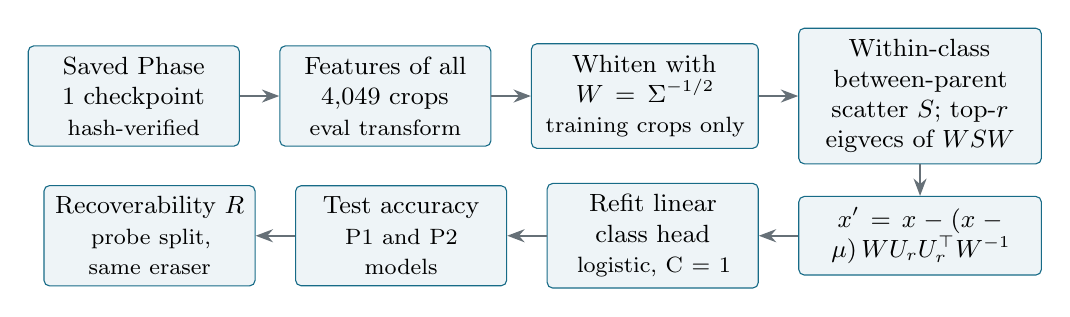
\begin{tikzpicture}[node distance=4mm and 5mm]
\node[box=24mm] (ckpt) {Saved Phase 1 checkpoint\\\footnotesize hash-verified};
\node[box=24mm, right=of ckpt] (feat) {Features of all 4,049 crops\\\footnotesize eval transform};
\node[box=26mm, right=of feat] (white) {Whiten with $W=\Sigma^{-1/2}$\\\footnotesize training crops only};
\node[box=28mm, right=of white] (scatter) {Within-class between-parent scatter $S$; top-$r$ eigvecs of $WSW$};
\node[box=28mm, below=of scatter] (erase) {$x' = x - (x-\mu)\,W U_r U_r^\top W^{-1}$};
\node[box=24mm, left=of erase] (refit) {Refit linear class head\\\footnotesize logistic, C = 1};
\node[box=24mm, left=of refit] (acc) {Test accuracy\\\footnotesize P1 and P2 models};
\node[box=24mm, left=of acc] (probe) {Recoverability $R$\\\footnotesize probe split, same eraser};
\draw[flow] (ckpt) -- (feat); \draw[flow] (feat) -- (white); \draw[flow] (white) -- (scatter); \draw[flow] (scatter) -- (erase);
\draw[flow] (erase) -- (refit); \draw[flow] (refit) -- (acc); \draw[flow] (acc) -- (probe);
\end{tikzpicture}
\end{adjustbox}
\caption{Rank-limited LEACE erasure (F5). At full rank the projection is LEACE for the within-class parent indicator:
no linear function of the erased features covaries with it on the fitting data. Ranks 0, 4, 16, 64, and 256 give the dose.}
\label{r:fig:leace}
\end{figure}


Every saved Phase~1 P1 and P2 model (480) is re-evaluated: features of all crops are extracted, the within-class parent
directions of the model's own training crops are erased at ranks 0, 4, 16, 64, and 256~\citep{belrose2023leace}, the class
head is refitted, and test accuracy and recoverability are measured. The regime and manipulation check follow H5. F5 asks
whether erasure at the strongest in-regime rank reduces the P1 $-$ P2 gap.

\section{F6: stain-normalisation dose}

Every crop is Reinhard-normalised toward one dataset-wide reference at strength 0.5 and 1.0, in training, test, and probe
crops alike. ResNet-50, ConvNeXt-T, DenseNet-121, and EfficientNet-B0 are trained on P1 and P2 for the ten Study~2 seeds no
mechanism arm used; strength 0 is the matching Phase~1 run. F6 is the reduction in gap per unit of strength.

\section{F7: probe-matched linear adversary}

The 2A design with a different adversary (Figure~\ref{r:fig:adversary}): per-feature standardisation and one linear layer,
its own optimiser at $10^{-3}$, re-initialised every five epochs. ResNet-50, ConvNeXt-T, and DenseNet-121; $\lambda\in\{0,
0.1, 0.3, 1, 3\}$; P1 and P2; the same ten seeds as F6. F7 is the slope of gap on recoverability, as for H5.

\section{F8: pooled dose-response}

All included architecture-by-level cells of F5, F6, and F7, after their regimes and manipulation checks:
$\text{gap}\sim\text{cell}+R_{\text{pair}}+(1\mid\text{manipulation:seed})$. F8 is the slope.

\section{Recoverability, measured the same way everywhere}

$R$ for F5--F8 is computed with one GPU implementation of the registered logistic probe (sklearn's objective, C = 1,
standardised features, L-BFGS). On the 280 Study~2 gradient-reversal runs it agreed with the registered sklearn probe at
$r=\ProbeAgreement$ (Figure~\ref{r:fig:probe-agreement}).

\begin{figure}[H]
\centering
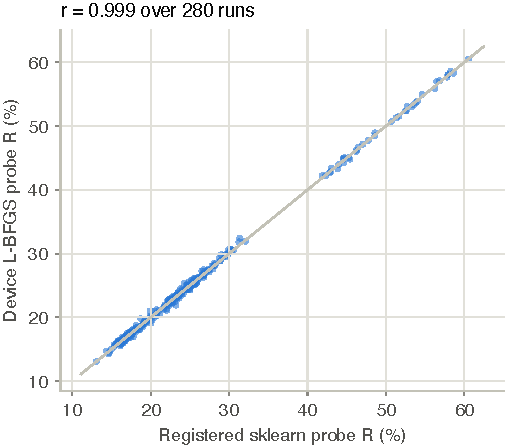
\includegraphics[width=0.55\textwidth]{probe_agreement.pdf}
\caption{Within-class recoverability from the registered sklearn probe and the device probe used for F5--F8, on the 280
Study~2 adversarial runs.}
\label{r:fig:probe-agreement}
\end{figure}

\chapter{Execution and the Amendment 9 fix}
\label{r:ch:a8-exec}

The new code was unit-tested on the workstation and, for GPU paths, on the host (13 tests, including a check that
full-rank erasure leaves no covariance between features and within-class parent identity, and that the device probe
matches sklearn to $10^{-3}$). A synthetic dry run of the registered models recovered every planted effect. Eleven smoke
tasks ran only on leak cells and single P1 runs; they confirmed that re-evaluated checkpoints reproduce their recorded
accuracy and that the linear adversary learns. The caches for masking, normalisation, and the ablations were built and
hashed, and the registration commit recorded every hash. The matrix of \RecFollowTasks\ tasks then ran from
\RecFollowStart\ to \RecFollowEnd\ without a failure.

\begin{warningbox}{Amendment 9: the preparer bug}
When the registered models were first run on the completed carrier arm, the R script stopped at F4: the preparer had
labelled all 160 standard-recipe runs as colour-augmented, because a missing colour augmentation (\texttt{None} in the run
record) became a NaN in a DataFrame row, and NaN is truthy. The script halted before writing any output, so no F3 or F4
estimate was seen. The condition is now read from each run record, a unit test covers it, and the fix was registered as
Amendment~9 (20 October, 01:25) before the corrected table was analysed. The synthetic dry run had bypassed the preparer,
which is why the bug was not caught earlier.
\end{warningbox}

\chapter{Follow-up results}
\label{r:ch:a8-results}

\small\begin{longtable}{lp{0.33\textwidth}rrrl}
\caption{The eight registered follow-up tests (one Holm family). Estimates are oriented so that the predicted direction is
positive.}\label{r:tab:a8-verdicts}\\
\toprule
& Question & Estimate & 95\% CI & Holm $p$ & Verdict \\
\midrule
\endfirsthead
\bottomrule
\endfoot
F1 & CRIC pull toward the slide's majority class & \FoneEst & \FoneLo\ to \FoneHi & \FonePholm & \notsupported \\
F2 & Stain transfer shrinks the leak effect & \FtwoEst & \FtwoLo\ to \FtwoHi & \FtwoPholm & \supported \\
F3 & Leak effect with backgrounds masked & \FthreeEst & \FthreeLo\ to \FthreeHi & \FthreePholm & \supported \\
F4 & Colour augmentation shrinks the leak effect & \FfourEst & \FfourLo\ to \FfourHi & \FfourPholm & \notsupported \\
F5 & LEACE erasure shrinks the gap & \FfiveEst & \FfiveLo\ to \FfiveHi & \FfivePholm & \notsupported \\
F6 & Stain normalisation shrinks the gap & \FsixEst & \FsixLo\ to \FsixHi & \FsixPholm & \notsupported \\
F7 & Gap tracks $R$ (linear adversary) & \FsevenEst & \FsevenLo\ to \FsevenHi & \FsevenPholm & \notsupported \\
F8 & Gap tracks $R$ (pooled) & \FeightEst & \FeightLo\ to \FeightHi & \FeightPholm & \notsupported \\
\end{longtable}

\section{The leak needs no background (F3)}

Trained and tested with every background replaced by a constant, leak models beat clean models by \FthreeEst~pp
(\FthreeLo--\FthreeHi; Holm $p$ \FthreePholm), at least as much as under the standard recipe on the same fresh seeds
(\CarrierStandard~pp), which also replicates H3 (\HthreeRepEst~pp, \HthreeRepLo--\HthreeRepHi). Masking changed the leak
effect by \MaskReductionEst~pp relative to standard training (\MaskReductionLo\ to \MaskReductionHi). At test time, removing
the background from the original 2C models' inputs left \RecBgKeep\% of their advantage.

\begin{figure}[H]
\centering
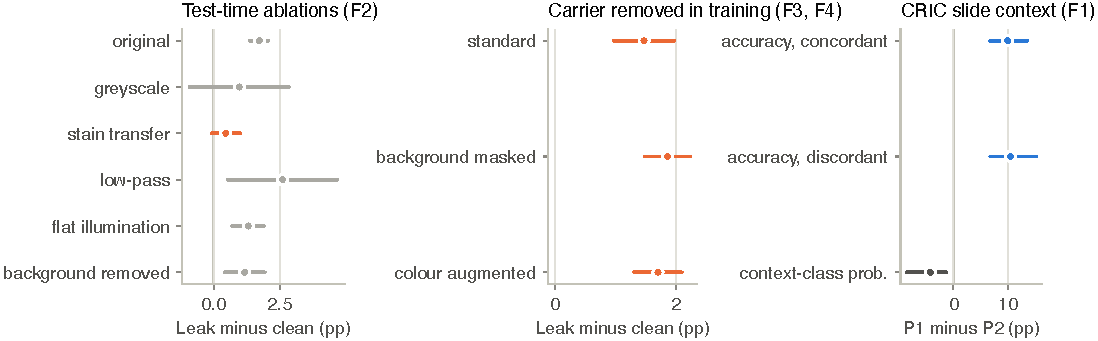
\includegraphics[width=\textwidth]{carriers.pdf}
\caption{Left: the leak advantage under each test-time ablation (F2 highlighted). Middle: the leak effect under each
training condition on fresh seeds (F3, F4). Right: CRIC within-cell accuracy gains by concordance, and the context-class
probability for discordant cells (F1).}
\label{r:fig:carriers}
\end{figure}

\begin{figure}[H]
\centering
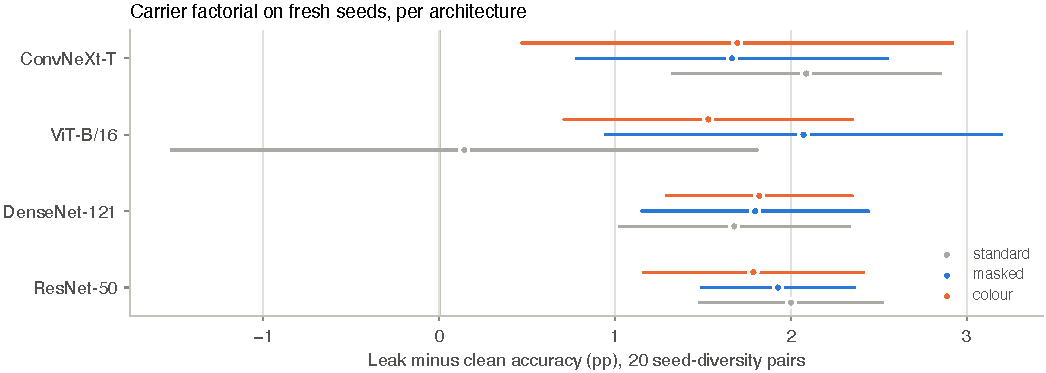
\includegraphics[width=\textwidth]{carrier_arch.pdf}
\caption{The carrier factorial per architecture.}
\label{r:fig:carrier-arch}
\end{figure}

{\scriptsize
\setlength{\tabcolsep}{3.5pt}
\begin{longtable}{llrrrrr}
\caption{Amendment 8 carrier factorial (fresh seeds, 10 per cell): accuracy per cell (percent) and the leak effect (pp).}\label{r:tab:carrier}\\
\toprule
Architecture & Condition & Leak high & Clean high & Leak low & Clean low & Leak effect \\
\midrule
\endfirsthead
\toprule
Architecture & Condition & Leak high & Clean high & Leak low & Clean low & Leak effect \\
\midrule
\endhead
\bottomrule
\endfoot
ResNet-50 & standard & 96.06\,$\pm$\,1.42 & 93.99\,$\pm$\,2.08 & 96.40\,$\pm$\,0.79 & 94.48\,$\pm$\,1.52 & 2.00 \\
 & masked & 95.46\,$\pm$\,1.19 & 93.42\,$\pm$\,1.26 & 95.69\,$\pm$\,1.36 & 93.87\,$\pm$\,1.37 & 1.92 \\
 & colour & 95.62\,$\pm$\,1.29 & 93.79\,$\pm$\,1.29 & 95.84\,$\pm$\,1.04 & 94.10\,$\pm$\,1.45 & 1.78 \\
DenseNet-121 & standard & 96.33\,$\pm$\,1.16 & 95.14\,$\pm$\,1.63 & 97.01\,$\pm$\,0.66 & 94.85\,$\pm$\,1.50 & 1.68 \\
 & masked & 95.59\,$\pm$\,1.32 & 94.21\,$\pm$\,1.00 & 96.19\,$\pm$\,0.87 & 93.99\,$\pm$\,1.84 & 1.79 \\
 & colour & 96.20\,$\pm$\,1.01 & 94.47\,$\pm$\,1.48 & 96.45\,$\pm$\,0.58 & 94.54\,$\pm$\,1.68 & 1.82 \\
ViT-B/16 & standard & 93.40\,$\pm$\,3.70 & 93.60\,$\pm$\,1.77 & 94.97\,$\pm$\,1.74 & 94.49\,$\pm$\,1.32 & 0.14 \\
 & masked & 94.92\,$\pm$\,2.21 & 92.95\,$\pm$\,1.97 & 94.91\,$\pm$\,1.13 & 92.74\,$\pm$\,1.56 & 2.07 \\
 & colour & 95.05\,$\pm$\,1.68 & 93.53\,$\pm$\,1.27 & 95.04\,$\pm$\,1.67 & 93.51\,$\pm$\,1.20 & 1.53 \\
ConvNeXt-T & standard & 96.56\,$\pm$\,0.95 & 95.05\,$\pm$\,1.23 & 96.66\,$\pm$\,0.67 & 94.00\,$\pm$\,2.32 & 2.08 \\
 & masked & 94.80\,$\pm$\,1.73 & 93.15\,$\pm$\,2.00 & 95.29\,$\pm$\,1.47 & 93.61\,$\pm$\,1.74 & 1.66 \\
 & colour & 95.30\,$\pm$\,1.77 & 94.24\,$\pm$\,1.95 & 95.77\,$\pm$\,1.51 & 93.44\,$\pm$\,2.68 & 1.69 \\
\end{longtable}
}


\section{The leak is tied to the field's colour rendering at test time (F2), but colour augmentation does not prevent it (F4)}

Moving each test cell's colour statistics to those of an unseen field of the same class cut the leak advantage from
\LeakUnderOriginal\ to \LeakUnderStain~pp, a reduction of \FtwoEst~pp (\FtwoLo--\FtwoHi; Holm $p=\FtwoPholm$), removing
\RecStainRemove\% of it. Interventions with comparable accuracy costs did not: with illumination flattened \RecFlatKeep\% of
the advantage remained, and with the background removed \RecBgKeep\%. Greyscale and low-pass filtering degraded accuracy too
far to be informative (Figure~\ref{r:fig:ablation-arch}). Yet models trained with strong colour augmentation leaked as much
as standard models (\CarrierColour\ versus \CarrierStandard~pp; F4 \FfourEst, \FfourLo\ to \FfourHi).

\begin{figure}[H]
\centering
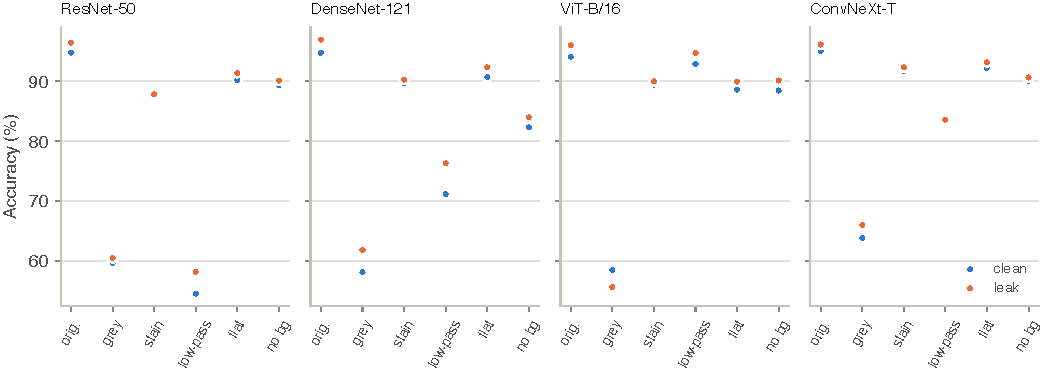
\includegraphics[width=\textwidth]{ablation_arch.pdf}
\caption{Accuracy of leak and clean 2C models under each test-time ablation, per architecture.}
\label{r:fig:ablation-arch}
\end{figure}

{\footnotesize
\setlength{\tabcolsep}{3.5pt}
\begin{longtable}{llrrr}
\caption{Amendment 8 test-time carrier ablations on the Study 2 2C models: leak and clean accuracy (percent, 20 runs each) and the leak advantage (pp).}\label{r:tab:ablation}\\
\toprule
Architecture & Ablation & Leak models & Clean models & Leak $-$ clean \\
\midrule
\endfirsthead
\toprule
Architecture & Ablation & Leak models & Clean models & Leak $-$ clean \\
\midrule
\endhead
\bottomrule
\endfoot
ResNet-50 & original & 96.45\,$\pm$\,0.94 & 94.77\,$\pm$\,1.33 & 1.69 \\
 & grey & 60.41\,$\pm$\,5.61 & 59.56\,$\pm$\,7.27 & 0.84 \\
 & stain\_transfer & 87.81\,$\pm$\,2.85 & 87.76\,$\pm$\,2.77 & 0.05 \\
 & low\_pass & 58.11\,$\pm$\,11.63 & 54.46\,$\pm$\,11.17 & 3.65 \\
 & illumination\_flat & 91.39\,$\pm$\,2.88 & 90.15\,$\pm$\,2.18 & 1.25 \\
 & background\_grey & 90.10\,$\pm$\,2.57 & 89.36\,$\pm$\,1.84 & 0.74 \\
DenseNet-121 & original & 96.94\,$\pm$\,0.78 & 94.73\,$\pm$\,1.50 & 2.21 \\
 & grey & 61.76\,$\pm$\,6.30 & 58.05\,$\pm$\,8.26 & 3.71 \\
 & stain\_transfer & 90.23\,$\pm$\,2.21 & 89.64\,$\pm$\,1.92 & 0.59 \\
 & low\_pass & 76.26\,$\pm$\,6.79 & 71.09\,$\pm$\,5.97 & 5.17 \\
 & illumination\_flat & 92.33\,$\pm$\,2.17 & 90.68\,$\pm$\,3.18 & 1.64 \\
 & background\_grey & 83.98\,$\pm$\,3.72 & 82.27\,$\pm$\,5.20 & 1.71 \\
ViT-B/16 & original & 96.01\,$\pm$\,1.15 & 94.08\,$\pm$\,2.01 & 1.93 \\
 & grey & 55.54\,$\pm$\,5.12 & 58.42\,$\pm$\,7.25 & \textminus{}2.87 \\
 & stain\_transfer & 89.97\,$\pm$\,2.40 & 89.40\,$\pm$\,3.25 & 0.57 \\
 & low\_pass & 94.70\,$\pm$\,1.74 & 92.87\,$\pm$\,2.95 & 1.83 \\
 & illumination\_flat & 89.90\,$\pm$\,2.63 & 88.56\,$\pm$\,3.56 & 1.34 \\
 & background\_grey & 90.12\,$\pm$\,2.73 & 88.44\,$\pm$\,3.54 & 1.68 \\
ConvNeXt-T & original & 96.14\,$\pm$\,1.38 & 95.08\,$\pm$\,1.49 & 1.06 \\
 & grey & 65.94\,$\pm$\,5.38 & 63.77\,$\pm$\,5.85 & 2.16 \\
 & stain\_transfer & 92.31\,$\pm$\,2.68 & 91.69\,$\pm$\,2.52 & 0.61 \\
 & low\_pass & 83.55\,$\pm$\,7.47 & 83.76\,$\pm$\,6.82 & \textminus{}0.20 \\
 & illumination\_flat & 93.20\,$\pm$\,1.62 & 92.21\,$\pm$\,1.87 & 0.98 \\
 & background\_grey & 90.59\,$\pm$\,2.46 & 90.03\,$\pm$\,1.98 & 0.56 \\
\end{longtable}
}


\section{Exploratory: not shared pixels}

In leak cells a third or more of the test crops overlap a training sibling in the source image. Splitting the leak
advantage by overlap (not registered) shows it is as large for crops that share no pixel with any training crop
(\OverlapNo~pp) as for crops that do (\OverlapYes~pp), in the Study~2 models and in all three carrier conditions; stain
transfer removed it in both subsets (\OverlapStainNo\ and \OverlapStainYes~pp). The leak generalises to new cells from a
seen field rather than reflecting memorised pixels.

\begin{figure}[H]
\centering
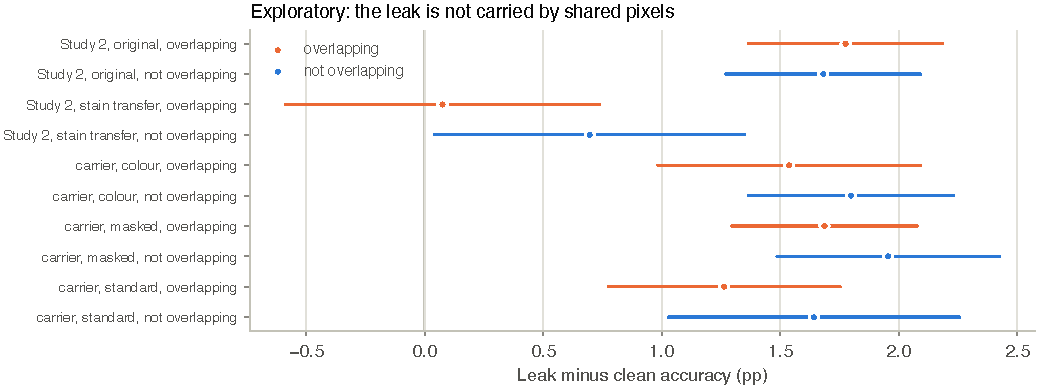
\includegraphics[width=\textwidth]{overlap.pdf}
\caption{Exploratory: the leak advantage on test crops that do or do not share source pixels with a training sibling.}
\label{r:fig:overlap}
\end{figure}

{\footnotesize
\setlength{\tabcolsep}{3.5pt}
\begin{longtable}{llrrrr}
\caption{EXPLORATORY (not registered): leak minus clean accuracy on test crops that do or do not share source pixels with a training sibling (pp; 95\% $t$ interval over architecture--seed--diversity pairs).}\label{r:tab:overlap}\\
\toprule
Condition & Subset & Pairs & Crops & Leak $-$ clean & 95\% CI \\
\midrule
\endfirsthead
\toprule
Condition & Subset & Pairs & Crops & Leak $-$ clean & 95\% CI \\
\midrule
\endhead
\bottomrule
\endfoot
Study 2, original & not overlapping & 80 & 320 & 1.68 & 1.27 to 2.09 \\
Study 2, original & overlapping & 80 & 207 & 1.78 & 1.37 to 2.19 \\
Study 2, stain transfer & not overlapping & 80 & 320 & 0.70 & 0.04 to 1.35 \\
Study 2, stain transfer & overlapping & 80 & 207 & 0.08 & \textminus{}0.59 to 0.74 \\
carrier, colour & not overlapping & 80 & 329 & 1.80 & 1.37 to 2.23 \\
carrier, colour & overlapping & 80 & 206 & 1.54 & 0.98 to 2.09 \\
carrier, masked & not overlapping & 80 & 329 & 1.96 & 1.49 to 2.42 \\
carrier, masked & overlapping & 80 & 206 & 1.69 & 1.30 to 2.08 \\
carrier, standard & not overlapping & 80 & 329 & 1.64 & 1.03 to 2.26 \\
carrier, standard & overlapping & 80 & 206 & 1.26 & 0.77 to 1.75 \\
\end{longtable}
}


\section{No slide-level label prior (F1)}

Over \FoneCells\ discordant CRIC cells from \FoneSlides\ slides, the probability of the slide's majority class was
\FoneEst~pp \emph{lower}, not higher, when the cell's slide was in training (\FoneLo\ to \FoneHi). All six architectures
showed the same sign. Crop-level training raised accuracy as much for discordant cells (\FoneDiscordant~pp) as for
concordant ones (\FoneConcordant~pp; contrast \FoneContrast~pp, \FoneContrastLo\ to \FoneContrastHi): seen slides help each
cell toward its own class, not toward the slide's typical class.

\begin{figure}[H]
\centering
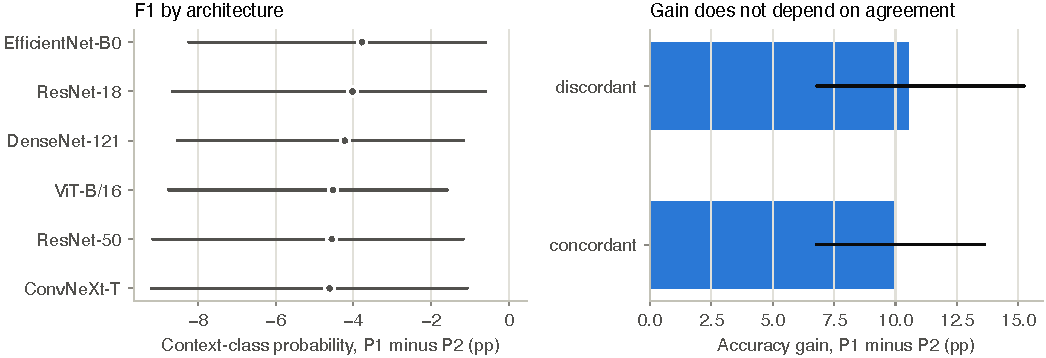
\includegraphics[width=\textwidth]{cric_context.pdf}
\caption{F1 per architecture, and the within-cell accuracy gain for concordant and discordant cells.}
\label{r:fig:cric-context}
\end{figure}

{\footnotesize
\setlength{\tabcolsep}{3.5pt}
\begin{longtable}{lrrrr}
\caption{F1 per architecture (secondary): within-cell P1 $-$ P2 context-class probability on discordant cells (pp) with slide-bootstrap intervals.}\label{r:tab:cricarch}\\
\toprule
Architecture & Estimate & 95\% CI & $p$ & Cells \\
\midrule
\endfirsthead
\toprule
Architecture & Estimate & 95\% CI & $p$ & Cells \\
\midrule
\endhead
\bottomrule
\endfoot
ConvNeXt-T & \textminus{}4.61 & \textminus{}9.19 to \textminus{}1.08 & 0.003 & 1,144 \\
DenseNet-121 & \textminus{}4.22 & \textminus{}8.52 to \textminus{}1.17 & 0.003 & 1,144 \\
EfficientNet-B0 & \textminus{}3.78 & \textminus{}8.22 to \textminus{}0.60 & 0.01 & 1,144 \\
ResNet-18 & \textminus{}4.02 & \textminus{}8.65 to \textminus{}0.61 & 0.01 & 1,144 \\
ResNet-50 & \textminus{}4.56 & \textminus{}9.15 to \textminus{}1.18 & 0.003 & 1,144 \\
ViT-B/16 & \textminus{}4.53 & \textminus{}8.75 to \textminus{}1.60 & $<$0.001 & 1,144 \\
\end{longtable}
}


\section{The gap does not track the fingerprint (F5--F8)}

\begin{figure}[H]
\centering
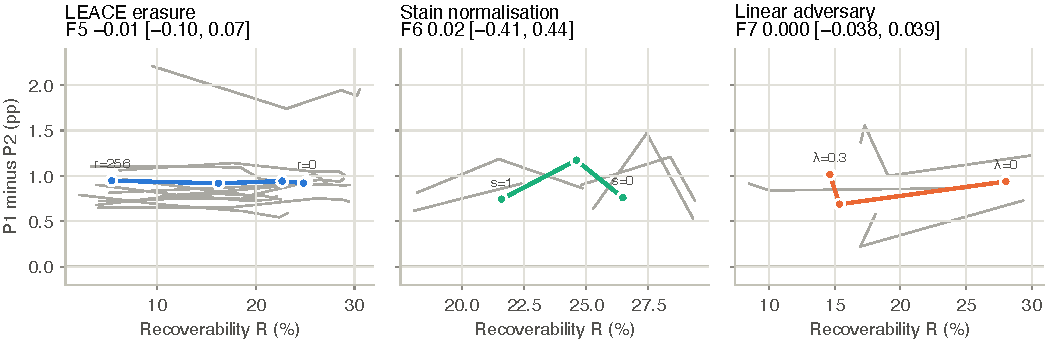
\includegraphics[width=\textwidth]{dose.pdf}
\caption{The P1 $-$ P2 gap against recoverability along three manipulations (grey: architectures; colour: pooled over
architectures that passed the manipulation check, at levels they share; registered in-regime levels only).}
\label{r:fig:dose}
\end{figure}

Rank-256 LEACE erasure cut recoverability from \LeaceRzero\% to \LeaceRtop\% (floor \RFloor\%) in all twelve architectures
while costing P2 \LeaceAccDrop~pp, and the gap stayed at \LeaceGapZero\ to \LeaceGapTop~pp (F5 \FfiveEst, \FfiveLo\ to
\FfiveHi). The probe-matched adversary passed its check in all three architectures, lowering $R$ from
\LinRzeroMin--\LinRzeroMax\% to \LinRstarMin--\LinRstarMax\% inside the regime, with a slope of \FsevenEst\ (\FsevenLo\ to
\FsevenHi). Stain normalisation lowered $R$ only from \NormRzero\% to \NormRtop\% while costing P2 \NormAccDrop~pp, failed
its check for every architecture, and left the gap unchanged (F6 \FsixEst, \FsixLo\ to \FsixHi). Pooled over the
\FeightCells\ included cells, the slope was \FeightEst\ (\FeightLo\ to \FeightHi): even a 20-pp loss of recoverability would
move the gap by at most about 0.1~pp.

\begin{figure}[H]
\centering
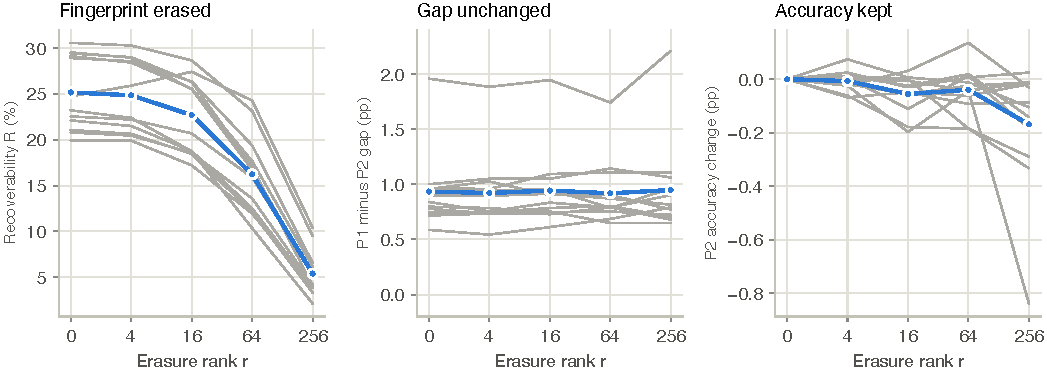
\includegraphics[width=\textwidth]{leace_full.pdf}
\caption{LEACE per architecture (grey) and pooled (blue): recoverability, gap, and P2 accuracy change by erasure rank.}
\label{r:fig:leace-full}
\end{figure}

\begin{figure}[H]
\centering
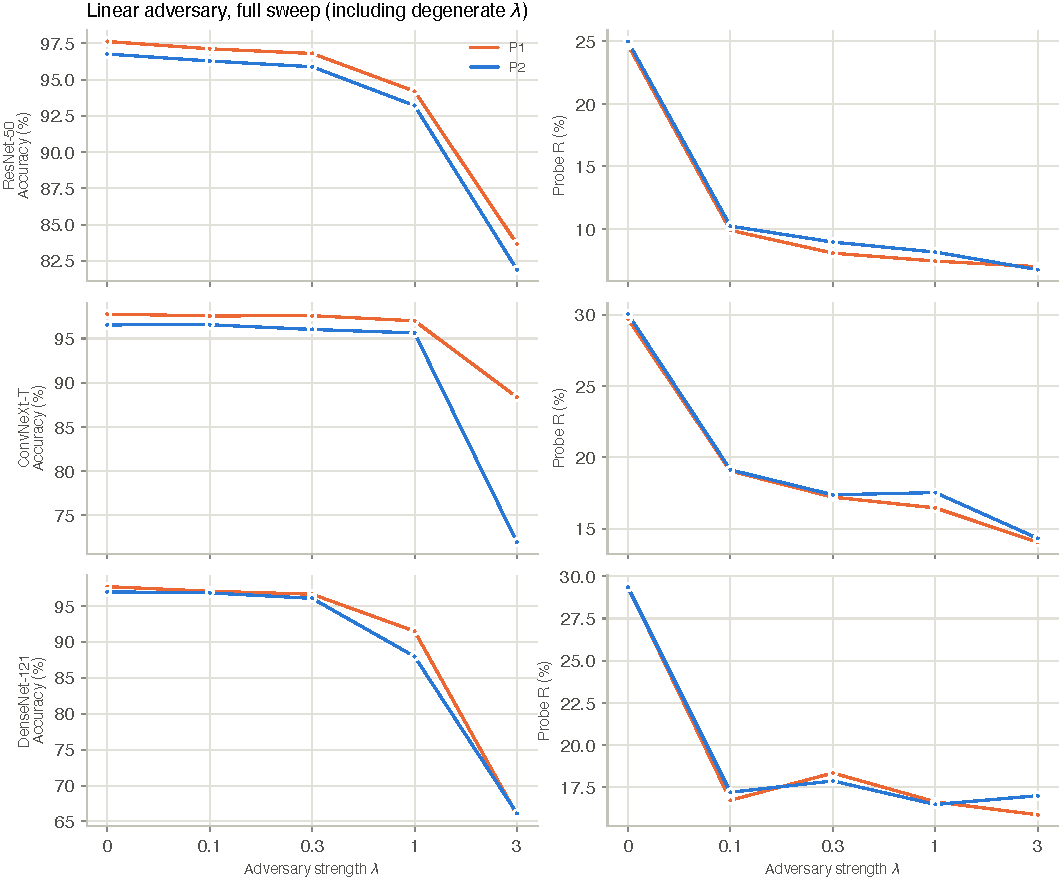
\includegraphics[width=\textwidth]{linadv_full.pdf}
\caption{The full linear-adversary sweep per architecture, including the degenerate strengths ($\lambda=1$ for ResNet-50
and DenseNet-121, $\lambda=3$ for all) where P2 accuracy collapses and which the regime rule excludes.}
\label{r:fig:linadv-full}
\end{figure}

\begin{figure}[H]
\centering
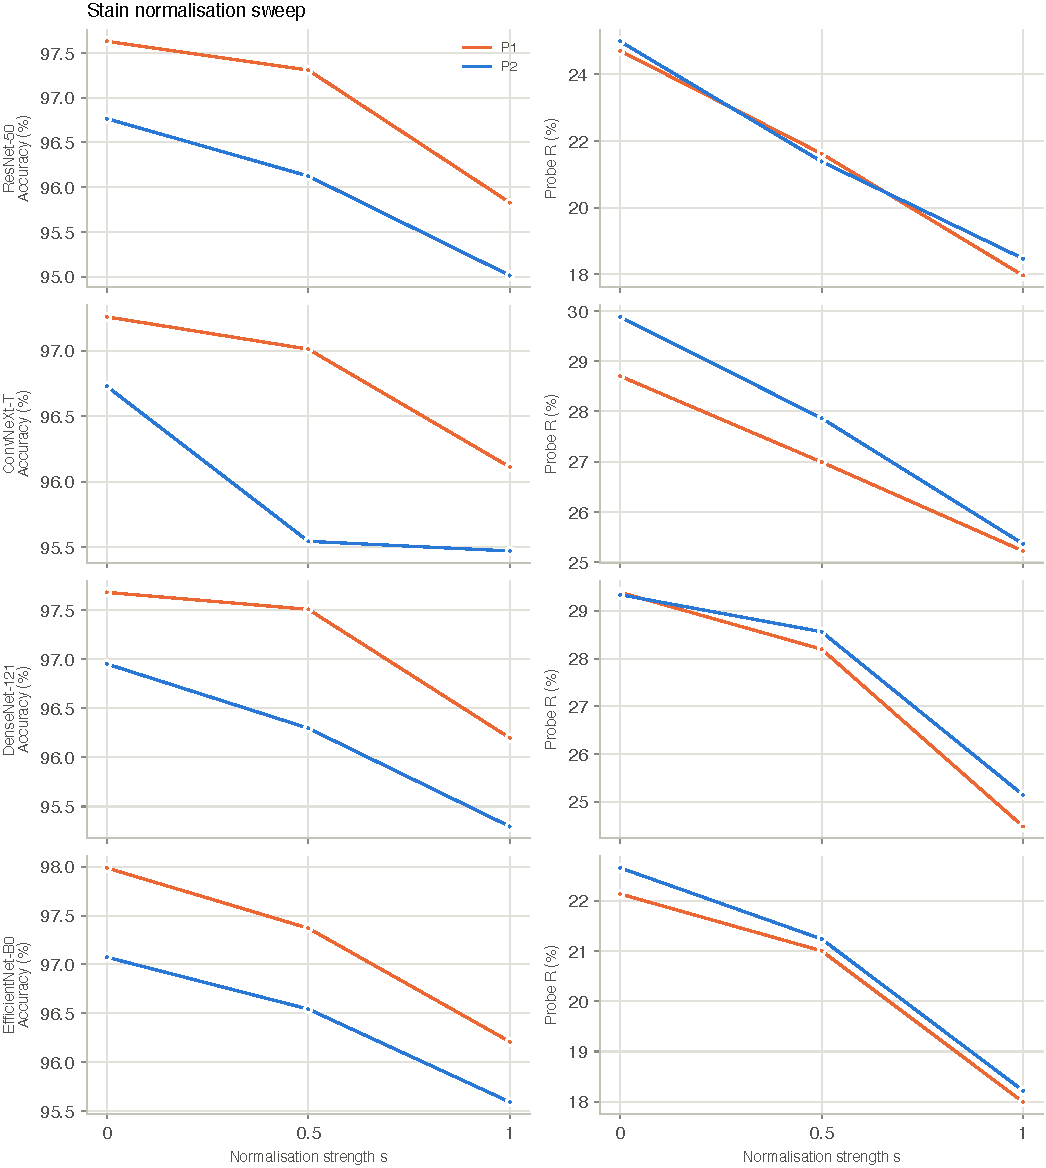
\includegraphics[width=\textwidth]{normalization_full.pdf}
\caption{The stain-normalisation sweep per architecture: accuracy falls for both protocols, recoverability falls only
modestly.}
\label{r:fig:normalization-full}
\end{figure}

{\scriptsize
\setlength{\tabcolsep}{3.5pt}
\begin{longtable}{llp{3.2cm}rrrrl}
\caption{Regimes and manipulation checks of every dose-response arm: levels whose mean P2 accuracy stays within 1 pp of baseline, the strongest such level, recoverability at baseline and there (percent), the class-only floor, and the check (at least a quarter of the above-floor $R$ removed).}\label{r:tab:checks}\\
\toprule
Arm & Architecture & Levels in regime & Strongest & $R_0$ & $R^*$ & Floor & Check \\
\midrule
\endfirsthead
\toprule
Arm & Architecture & Levels in regime & Strongest & $R_0$ & $R^*$ & Floor & Check \\
\midrule
\endhead
\bottomrule
\endfoot
H5 GRL & ResNet-50 & 0, 0.01, 0.03, 0.1, 0.3, 1, 3 & 3 & 24.7 & 17.6 & 1.2 & \pass \\
 & ConvNeXt-T & 0, 0.01, 0.03, 0.1, 0.3, 1, 3 & 3 & 29.5 & 55.1 & 1.2 & \fail \\
F5 LEACE & ResNet-18 & 0, 4, 16, 64, 256 & 256 & 23.2 & 2.1 & 1.2 & \pass \\
 & ResNet-50 & 0, 4, 16, 64, 256 & 256 & 24.7 & 10.4 & 1.2 & \pass \\
 & DenseNet-121 & 0, 4, 16, 64, 256 & 256 & 29.4 & 4.1 & 1.2 & \pass \\
 & EfficientNet-B0 & 0, 4, 16, 64, 256 & 256 & 22.5 & 5.5 & 1.2 & \pass \\
 & MobileNet-V2 & 0, 4, 16, 64, 256 & 256 & 20.8 & 4.2 & 1.2 & \pass \\
 & ViT-B/16 & 0, 4, 16, 64, 256 & 256 & 29.1 & 6.2 & 1.2 & \pass \\
 & ConvNeXt-T & 0, 4, 16, 64, 256 & 256 & 29.5 & 5.2 & 1.2 & \pass \\
 & Swin-T & 0, 4, 16, 64, 256 & 256 & 28.9 & 6.6 & 1.2 & \pass \\
 & RegNetY-1.6GF & 0, 4, 16, 64, 256 & 256 & 21.1 & 3.4 & 1.2 & \pass \\
 & EfficientNetV2-S & 0, 4, 16, 64, 256 & 256 & 19.9 & 3.9 & 1.2 & \pass \\
 & MaxViT-T & 0, 4, 16, 64, 256 & 256 & 22.1 & 3.9 & 1.2 & \pass \\
 & DINOv2 ViT-S/14 & 0, 4, 16, 64, 256 & 256 & 30.5 & 9.5 & 1.2 & \pass \\
F6 normalisation & ResNet-50 & 0, 0.5 & 0.5 & 24.8 & 21.5 & 1.2 & \fail \\
 & DenseNet-121 & 0, 0.5 & 0.5 & 29.4 & 28.4 & 1.2 & \fail \\
 & EfficientNet-B0 & 0, 0.5 & 0.5 & 22.4 & 21.1 & 1.2 & \fail \\
 & ConvNeXt-T & 0 & 0 & 29.3 & 29.3 & 1.2 & \fail \\
F7 linear adv. & ResNet-50 & 0, 0.1, 0.3 & 0.3 & 24.8 & 8.5 & 1.2 & \pass \\
 & DenseNet-121 & 0, 0.1, 0.3 & 0.3 & 29.4 & 18.1 & 1.2 & \pass \\
 & ConvNeXt-T & 0, 0.1, 0.3, 1 & 1 & 29.9 & 17.0 & 1.2 & \pass \\
\end{longtable}
}

{\scriptsize
\setlength{\tabcolsep}{3.5pt}
\begin{longtable}{lrrrrrrr}
\caption{Amendment 8 rank-limited LEACE erasure on every Phase 1 model (20 seeds): accuracy with a refitted head (percent), gap (pp), logistic recoverability $R$, and nearest-centroid recoverability (percent).}\label{r:tab:leace}\\
\toprule
Architecture & Rank & P1 acc. & P2 acc. & Gap & $R$ (P1) & $R$ (P2) & NCC \\
\midrule
\endfirsthead
\toprule
Architecture & Rank & P1 acc. & P2 acc. & Gap & $R$ (P1) & $R$ (P2) & NCC \\
\midrule
\endhead
\bottomrule
\endfoot
ResNet-18 & 0 & 97.90\,$\pm$\,0.37 & 97.31\,$\pm$\,0.61 & 0.59 & 23.1\,$\pm$\,1.2 & 23.2\,$\pm$\,1.1 & 21.0\,$\pm$\,1.0 \\
 & 4 & 97.86\,$\pm$\,0.37 & 97.32\,$\pm$\,0.68 & 0.54 & 22.2\,$\pm$\,1.2 & 22.5\,$\pm$\,1.1 & 19.6\,$\pm$\,1.1 \\
 & 16 & 97.92\,$\pm$\,0.38 & 97.31\,$\pm$\,0.70 & 0.61 & 18.7\,$\pm$\,1.1 & 18.7\,$\pm$\,1.0 & 15.2\,$\pm$\,1.1 \\
 & 64 & 97.81\,$\pm$\,0.37 & 97.12\,$\pm$\,0.81 & 0.69 & 10.5\,$\pm$\,0.8 & 10.2\,$\pm$\,1.0 & 8.1\,$\pm$\,0.8 \\
 & 256 & 97.77\,$\pm$\,0.33 & 96.98\,$\pm$\,1.00 & 0.79 & 2.0\,$\pm$\,0.4 & 2.3\,$\pm$\,0.5 & 1.8\,$\pm$\,0.4 \\
ResNet-50 & 0 & 98.12\,$\pm$\,0.42 & 97.16\,$\pm$\,0.67 & 0.96 & 24.6\,$\pm$\,1.1 & 24.9\,$\pm$\,1.1 & 23.0\,$\pm$\,1.2 \\
 & 4 & 98.12\,$\pm$\,0.45 & 97.09\,$\pm$\,0.72 & 1.02 & 25.9\,$\pm$\,1.5 & 25.9\,$\pm$\,1.2 & 23.5\,$\pm$\,1.2 \\
 & 16 & 98.01\,$\pm$\,0.46 & 97.11\,$\pm$\,0.67 & 0.90 & 27.6\,$\pm$\,1.6 & 27.2\,$\pm$\,1.2 & 24.1\,$\pm$\,1.4 \\
 & 64 & 98.00\,$\pm$\,0.43 & 97.10\,$\pm$\,0.76 & 0.90 & 24.6\,$\pm$\,1.8 & 23.9\,$\pm$\,1.1 & 19.9\,$\pm$\,1.2 \\
 & 256 & 97.91\,$\pm$\,0.43 & 97.14\,$\pm$\,0.72 & 0.77 & 10.7\,$\pm$\,0.9 & 10.1\,$\pm$\,0.8 & 8.7\,$\pm$\,0.8 \\
DenseNet-121 & 0 & 98.24\,$\pm$\,0.32 & 97.52\,$\pm$\,0.67 & 0.72 & 29.5\,$\pm$\,1.3 & 29.2\,$\pm$\,1.3 & 23.7\,$\pm$\,1.3 \\
 & 4 & 98.27\,$\pm$\,0.30 & 97.53\,$\pm$\,0.64 & 0.73 & 29.1\,$\pm$\,1.1 & 28.9\,$\pm$\,1.2 & 22.8\,$\pm$\,1.2 \\
 & 16 & 98.17\,$\pm$\,0.35 & 97.41\,$\pm$\,0.73 & 0.75 & 26.2\,$\pm$\,1.3 & 26.4\,$\pm$\,0.9 & 18.8\,$\pm$\,1.3 \\
 & 64 & 98.19\,$\pm$\,0.25 & 97.54\,$\pm$\,0.78 & 0.65 & 17.1\,$\pm$\,0.8 & 17.0\,$\pm$\,1.2 & 10.8\,$\pm$\,1.1 \\
 & 256 & 97.99\,$\pm$\,0.35 & 97.34\,$\pm$\,0.74 & 0.65 & 3.7\,$\pm$\,0.6 & 4.4\,$\pm$\,0.6 & 2.6\,$\pm$\,0.6 \\
EfficientNet-B0 & 0 & 98.04\,$\pm$\,0.54 & 97.30\,$\pm$\,0.88 & 0.74 & 22.3\,$\pm$\,1.1 & 22.8\,$\pm$\,1.3 & 20.1\,$\pm$\,1.2 \\
 & 4 & 98.05\,$\pm$\,0.53 & 97.30\,$\pm$\,0.87 & 0.75 & 22.0\,$\pm$\,1.0 & 22.4\,$\pm$\,1.4 & 19.5\,$\pm$\,1.2 \\
 & 16 & 98.08\,$\pm$\,0.55 & 97.30\,$\pm$\,0.91 & 0.78 & 20.6\,$\pm$\,1.3 & 20.8\,$\pm$\,1.4 & 17.3\,$\pm$\,1.2 \\
 & 64 & 98.06\,$\pm$\,0.48 & 97.26\,$\pm$\,0.94 & 0.80 & 16.1\,$\pm$\,1.2 & 15.7\,$\pm$\,1.3 & 12.0\,$\pm$\,1.1 \\
 & 256 & 97.99\,$\pm$\,0.49 & 97.29\,$\pm$\,0.75 & 0.70 & 5.5\,$\pm$\,0.8 & 5.5\,$\pm$\,0.9 & 4.2\,$\pm$\,0.6 \\
MobileNet-V2 & 0 & 97.41\,$\pm$\,0.48 & 96.61\,$\pm$\,0.88 & 0.80 & 20.6\,$\pm$\,1.2 & 21.0\,$\pm$\,0.9 & 19.3\,$\pm$\,1.1 \\
 & 4 & 97.41\,$\pm$\,0.52 & 96.62\,$\pm$\,0.91 & 0.78 & 20.2\,$\pm$\,1.0 & 20.7\,$\pm$\,1.1 & 18.3\,$\pm$\,1.0 \\
 & 16 & 97.33\,$\pm$\,0.58 & 96.59\,$\pm$\,0.91 & 0.75 & 18.5\,$\pm$\,1.2 & 18.7\,$\pm$\,1.0 & 15.5\,$\pm$\,1.2 \\
 & 64 & 97.38\,$\pm$\,0.56 & 96.63\,$\pm$\,0.85 & 0.75 & 13.7\,$\pm$\,1.0 & 13.5\,$\pm$\,0.9 & 10.8\,$\pm$\,0.9 \\
 & 256 & 97.19\,$\pm$\,0.49 & 96.47\,$\pm$\,0.80 & 0.72 & 4.2\,$\pm$\,0.8 & 4.2\,$\pm$\,0.6 & 3.5\,$\pm$\,0.6 \\
ViT-B/16 & 0 & 97.83\,$\pm$\,0.75 & 96.83\,$\pm$\,0.80 & 1.00 & 28.8\,$\pm$\,1.2 & 29.4\,$\pm$\,1.2 & 25.1\,$\pm$\,1.3 \\
 & 4 & 97.86\,$\pm$\,0.71 & 96.81\,$\pm$\,0.74 & 1.05 & 28.1\,$\pm$\,1.3 & 28.7\,$\pm$\,1.1 & 23.9\,$\pm$\,1.4 \\
 & 16 & 97.83\,$\pm$\,0.72 & 96.78\,$\pm$\,0.82 & 1.05 & 25.3\,$\pm$\,1.4 & 25.8\,$\pm$\,1.1 & 19.9\,$\pm$\,1.3 \\
 & 64 & 97.88\,$\pm$\,0.68 & 96.73\,$\pm$\,0.76 & 1.14 & 17.6\,$\pm$\,1.3 & 17.7\,$\pm$\,1.4 & 12.7\,$\pm$\,1.2 \\
 & 256 & 97.80\,$\pm$\,0.72 & 96.74\,$\pm$\,0.70 & 1.06 & 6.1\,$\pm$\,0.7 & 6.3\,$\pm$\,1.0 & 4.6\,$\pm$\,0.6 \\
ConvNeXt-T & 0 & 98.20\,$\pm$\,0.36 & 97.30\,$\pm$\,0.72 & 0.90 & 29.3\,$\pm$\,1.3 & 29.7\,$\pm$\,1.5 & 26.3\,$\pm$\,1.6 \\
 & 4 & 98.17\,$\pm$\,0.40 & 97.28\,$\pm$\,0.67 & 0.90 & 28.8\,$\pm$\,1.3 & 29.0\,$\pm$\,1.4 & 25.1\,$\pm$\,1.6 \\
 & 16 & 98.15\,$\pm$\,0.44 & 97.24\,$\pm$\,0.80 & 0.91 & 25.5\,$\pm$\,1.2 & 25.6\,$\pm$\,1.5 & 20.8\,$\pm$\,1.5 \\
 & 64 & 98.14\,$\pm$\,0.37 & 97.27\,$\pm$\,0.73 & 0.87 & 16.8\,$\pm$\,1.1 & 16.6\,$\pm$\,1.1 & 13.0\,$\pm$\,0.9 \\
 & 256 & 98.10\,$\pm$\,0.38 & 97.28\,$\pm$\,0.74 & 0.81 & 5.1\,$\pm$\,0.6 & 5.3\,$\pm$\,0.7 & 4.0\,$\pm$\,0.6 \\
Swin-T & 0 & 98.17\,$\pm$\,0.50 & 97.20\,$\pm$\,0.81 & 0.97 & 29.0\,$\pm$\,1.4 & 28.8\,$\pm$\,1.5 & 25.5\,$\pm$\,1.4 \\
 & 4 & 98.12\,$\pm$\,0.49 & 97.18\,$\pm$\,0.80 & 0.94 & 28.7\,$\pm$\,1.4 & 28.4\,$\pm$\,1.4 & 24.9\,$\pm$\,1.3 \\
 & 16 & 98.19\,$\pm$\,0.48 & 97.23\,$\pm$\,0.77 & 0.96 & 26.5\,$\pm$\,1.1 & 26.2\,$\pm$\,1.5 & 22.0\,$\pm$\,1.4 \\
 & 64 & 98.12\,$\pm$\,0.52 & 97.34\,$\pm$\,0.79 & 0.78 & 19.6\,$\pm$\,1.3 & 19.2\,$\pm$\,1.3 & 15.0\,$\pm$\,1.2 \\
 & 256 & 98.14\,$\pm$\,0.41 & 97.17\,$\pm$\,0.61 & 0.96 & 6.5\,$\pm$\,0.8 & 6.7\,$\pm$\,0.8 & 5.2\,$\pm$\,0.8 \\
RegNetY-1.6GF & 0 & 97.87\,$\pm$\,0.46 & 96.91\,$\pm$\,0.83 & 0.96 & 21.0\,$\pm$\,1.4 & 21.1\,$\pm$\,1.1 & 19.4\,$\pm$\,1.2 \\
 & 4 & 97.80\,$\pm$\,0.42 & 96.85\,$\pm$\,0.83 & 0.96 & 20.5\,$\pm$\,1.3 & 20.8\,$\pm$\,1.4 & 18.9\,$\pm$\,1.1 \\
 & 16 & 97.82\,$\pm$\,0.49 & 96.73\,$\pm$\,0.85 & 1.09 & 18.5\,$\pm$\,1.4 & 18.4\,$\pm$\,1.3 & 15.8\,$\pm$\,1.1 \\
 & 64 & 97.83\,$\pm$\,0.44 & 96.72\,$\pm$\,0.92 & 1.10 & 12.3\,$\pm$\,1.1 & 11.9\,$\pm$\,1.0 & 9.9\,$\pm$\,1.0 \\
 & 256 & 97.72\,$\pm$\,0.42 & 96.62\,$\pm$\,0.85 & 1.10 & 3.3\,$\pm$\,0.7 & 3.4\,$\pm$\,0.6 & 2.7\,$\pm$\,0.7 \\
EfficientNetV2-S & 0 & 97.70\,$\pm$\,0.50 & 96.86\,$\pm$\,1.01 & 0.84 & 19.5\,$\pm$\,1.4 & 20.4\,$\pm$\,1.5 & 17.6\,$\pm$\,1.1 \\
 & 4 & 97.69\,$\pm$\,0.48 & 96.93\,$\pm$\,0.93 & 0.75 & 19.5\,$\pm$\,1.7 & 20.2\,$\pm$\,1.3 & 15.6\,$\pm$\,3.1 \\
 & 16 & 97.70\,$\pm$\,0.51 & 96.86\,$\pm$\,0.89 & 0.83 & 16.7\,$\pm$\,2.1 & 17.8\,$\pm$\,2.0 & 11.5\,$\pm$\,4.2 \\
 & 64 & 97.64\,$\pm$\,0.61 & 96.85\,$\pm$\,0.97 & 0.79 & 11.0\,$\pm$\,3.3 & 12.9\,$\pm$\,2.7 & 7.6\,$\pm$\,3.7 \\
 & 256 & 97.65\,$\pm$\,0.51 & 96.75\,$\pm$\,0.91 & 0.90 & 3.4\,$\pm$\,1.3 & 4.4\,$\pm$\,1.1 & 2.9\,$\pm$\,1.1 \\
MaxViT-T & 0 & 97.88\,$\pm$\,0.46 & 97.10\,$\pm$\,0.83 & 0.78 & 21.6\,$\pm$\,1.2 & 22.6\,$\pm$\,1.5 & 19.1\,$\pm$\,1.3 \\
 & 4 & 97.86\,$\pm$\,0.46 & 97.12\,$\pm$\,0.87 & 0.73 & 20.9\,$\pm$\,1.3 & 22.0\,$\pm$\,1.5 & 18.2\,$\pm$\,1.4 \\
 & 16 & 97.80\,$\pm$\,0.49 & 97.07\,$\pm$\,0.86 & 0.73 & 18.3\,$\pm$\,1.2 & 19.2\,$\pm$\,1.7 & 14.8\,$\pm$\,1.4 \\
 & 64 & 97.90\,$\pm$\,0.49 & 97.10\,$\pm$\,0.86 & 0.79 & 12.4\,$\pm$\,1.0 & 12.6\,$\pm$\,1.7 & 9.4\,$\pm$\,1.0 \\
 & 256 & 97.80\,$\pm$\,0.42 & 97.12\,$\pm$\,0.79 & 0.68 & 3.8\,$\pm$\,0.5 & 4.0\,$\pm$\,0.9 & 3.1\,$\pm$\,0.6 \\
DINOv2 ViT-S/14 & 0 & 95.91\,$\pm$\,0.75 & 93.96\,$\pm$\,1.01 & 1.96 & 30.8\,$\pm$\,0.9 & 30.3\,$\pm$\,1.4 & 26.9\,$\pm$\,1.3 \\
 & 4 & 95.81\,$\pm$\,0.79 & 93.93\,$\pm$\,1.02 & 1.88 & 30.5\,$\pm$\,0.9 & 30.0\,$\pm$\,1.4 & 26.1\,$\pm$\,1.4 \\
 & 16 & 95.70\,$\pm$\,0.76 & 93.76\,$\pm$\,0.97 & 1.94 & 28.4\,$\pm$\,1.1 & 28.9\,$\pm$\,1.3 & 23.8\,$\pm$\,1.4 \\
 & 64 & 95.65\,$\pm$\,0.73 & 93.91\,$\pm$\,1.00 & 1.74 & 23.2\,$\pm$\,1.4 & 23.0\,$\pm$\,1.4 & 16.8\,$\pm$\,1.5 \\
 & 256 & 95.33\,$\pm$\,0.98 & 93.12\,$\pm$\,1.17 & 2.21 & 9.3\,$\pm$\,0.8 & 9.8\,$\pm$\,1.2 & 6.3\,$\pm$\,1.0 \\
\end{longtable}
}

{\footnotesize
\setlength{\tabcolsep}{3.5pt}
\begin{longtable}{lrrrrrr}
\caption{Amendment 8 probe-matched linear adversary (10 seeds): accuracy (percent), gap (pp), and recoverability $R$ (percent; device probe). $\lambda$ above the regime collapses P2 accuracy.}\label{r:tab:linadv}\\
\toprule
Architecture & $\lambda$ & P1 acc. & P2 acc. & Gap & $R$ (P1) & $R$ (P2) \\
\midrule
\endfirsthead
\toprule
Architecture & $\lambda$ & P1 acc. & P2 acc. & Gap & $R$ (P1) & $R$ (P2) \\
\midrule
\endhead
\bottomrule
\endfoot
ResNet-50 & 0 & 97.63\,$\pm$\,0.48 & 96.77\,$\pm$\,0.71 & 0.86 & 24.7\,$\pm$\,1.2 & 25.0\,$\pm$\,0.9 \\
 & 0.1 & 97.12\,$\pm$\,0.29 & 96.28\,$\pm$\,0.44 & 0.84 & 9.9\,$\pm$\,1.1 & 10.2\,$\pm$\,0.9 \\
 & 0.3 & 96.80\,$\pm$\,0.78 & 95.89\,$\pm$\,0.73 & 0.91 & 8.1\,$\pm$\,1.1 & 9.0\,$\pm$\,1.1 \\
 & 1 & 94.20\,$\pm$\,1.88 & 93.21\,$\pm$\,1.61 & 0.99 & 7.4\,$\pm$\,1.3 & 8.1\,$\pm$\,1.4 \\
 & 3 & 83.67\,$\pm$\,8.43 & 81.89\,$\pm$\,8.69 & 1.78 & 7.0\,$\pm$\,1.6 & 6.7\,$\pm$\,1.3 \\
DenseNet-121 & 0 & 97.68\,$\pm$\,0.55 & 96.95\,$\pm$\,0.35 & 0.73 & 29.4\,$\pm$\,1.3 & 29.3\,$\pm$\,1.6 \\
 & 0.1 & 97.04\,$\pm$\,0.60 & 96.81\,$\pm$\,0.77 & 0.22 & 16.7\,$\pm$\,1.4 & 17.2\,$\pm$\,1.5 \\
 & 0.3 & 96.63\,$\pm$\,1.10 & 96.05\,$\pm$\,1.30 & 0.58 & 18.3\,$\pm$\,1.5 & 17.9\,$\pm$\,1.0 \\
 & 1 & 91.48\,$\pm$\,2.44 & 87.96\,$\pm$\,5.59 & 3.52 & 16.6\,$\pm$\,1.0 & 16.5\,$\pm$\,1.8 \\
 & 3 & 65.93\,$\pm$\,7.69 & 66.11\,$\pm$\,9.63 & \textminus{}0.19 & 15.9\,$\pm$\,2.6 & 17.0\,$\pm$\,1.1 \\
ConvNeXt-T & 0 & 97.77\,$\pm$\,0.73 & 96.54\,$\pm$\,0.75 & 1.22 & 29.7\,$\pm$\,1.4 & 30.0\,$\pm$\,1.1 \\
 & 0.1 & 97.56\,$\pm$\,0.75 & 96.56\,$\pm$\,0.78 & 1.00 & 19.0\,$\pm$\,1.4 & 19.1\,$\pm$\,1.6 \\
 & 0.3 & 97.58\,$\pm$\,0.65 & 96.02\,$\pm$\,1.80 & 1.56 & 17.2\,$\pm$\,1.2 & 17.4\,$\pm$\,1.2 \\
 & 1 & 97.00\,$\pm$\,0.69 & 95.63\,$\pm$\,1.18 & 1.37 & 16.5\,$\pm$\,1.9 & 17.5\,$\pm$\,1.5 \\
 & 3 & 88.36\,$\pm$\,3.04 & 71.95\,$\pm$\,28.54 & 16.41 & 14.0\,$\pm$\,1.7 & 14.3\,$\pm$\,3.7 \\
\end{longtable}
}

{\footnotesize
\setlength{\tabcolsep}{3.5pt}
\begin{longtable}{lrrrrrr}
\caption{Amendment 8 Reinhard stain normalisation (10 seeds; strength 0 is the matching Phase 1 run): accuracy (percent), gap (pp), and $R$ (percent).}\label{r:tab:normal}\\
\toprule
Architecture & $s$ & P1 acc. & P2 acc. & Gap & $R$ (P1) & $R$ (P2) \\
\midrule
\endfirsthead
\toprule
Architecture & $s$ & P1 acc. & P2 acc. & Gap & $R$ (P1) & $R$ (P2) \\
\midrule
\endhead
\bottomrule
\endfoot
ResNet-50 & 0 & 97.63\,$\pm$\,0.48 & 96.77\,$\pm$\,0.71 & 0.86 & 24.7\,$\pm$\,1.2 & 25.0\,$\pm$\,0.9 \\
 & 0.5 & 97.31\,$\pm$\,0.58 & 96.12\,$\pm$\,0.68 & 1.19 & 21.6\,$\pm$\,0.7 & 21.4\,$\pm$\,0.9 \\
 & 1 & 95.83\,$\pm$\,0.39 & 95.01\,$\pm$\,1.40 & 0.81 & 18.0\,$\pm$\,1.0 & 18.5\,$\pm$\,1.1 \\
DenseNet-121 & 0 & 97.68\,$\pm$\,0.55 & 96.95\,$\pm$\,0.35 & 0.73 & 29.4\,$\pm$\,1.3 & 29.3\,$\pm$\,1.6 \\
 & 0.5 & 97.51\,$\pm$\,0.47 & 96.30\,$\pm$\,0.61 & 1.21 & 28.2\,$\pm$\,1.1 & 28.6\,$\pm$\,1.4 \\
 & 1 & 96.20\,$\pm$\,0.83 & 95.30\,$\pm$\,0.92 & 0.90 & 24.5\,$\pm$\,1.0 & 25.1\,$\pm$\,0.9 \\
EfficientNet-B0 & 0 & 97.99\,$\pm$\,0.39 & 97.07\,$\pm$\,0.52 & 0.91 & 22.1\,$\pm$\,1.2 & 22.7\,$\pm$\,1.1 \\
 & 0.5 & 97.37\,$\pm$\,0.56 & 96.54\,$\pm$\,0.60 & 0.83 & 21.0\,$\pm$\,1.6 & 21.2\,$\pm$\,1.6 \\
 & 1 & 96.21\,$\pm$\,0.56 & 95.59\,$\pm$\,1.13 & 0.62 & 18.0\,$\pm$\,1.2 & 18.2\,$\pm$\,0.9 \\
ConvNeXt-T & 0 & 97.26\,$\pm$\,0.63 & 96.73\,$\pm$\,0.46 & 0.53 & 28.7\,$\pm$\,1.2 & 29.9\,$\pm$\,1.5 \\
 & 0.5 & 97.01\,$\pm$\,0.76 & 95.54\,$\pm$\,1.44 & 1.47 & 27.0\,$\pm$\,2.0 & 27.9\,$\pm$\,1.0 \\
 & 1 & 96.11\,$\pm$\,1.24 & 95.47\,$\pm$\,1.06 & 0.64 & 25.2\,$\pm$\,1.9 & 25.4\,$\pm$\,1.1 \\
\end{longtable}
}


\section{Grad-CAM sees no difference}

Leak and clean models placed the same share of Grad-CAM attribution outside the cell mask (\CamBgAttribution\% on average,
against a background pixel share of \CamBgPixels\%; leak minus clean \CamLeakEst~pp, \CamLeakLo\ to \CamLeakHi). The maps
depended on the trained head (median Spearman \CamSpearman\ with a random-head map), so the absence of a difference is not a
failure of the method's sanity check.

\begin{figure}[H]
\centering
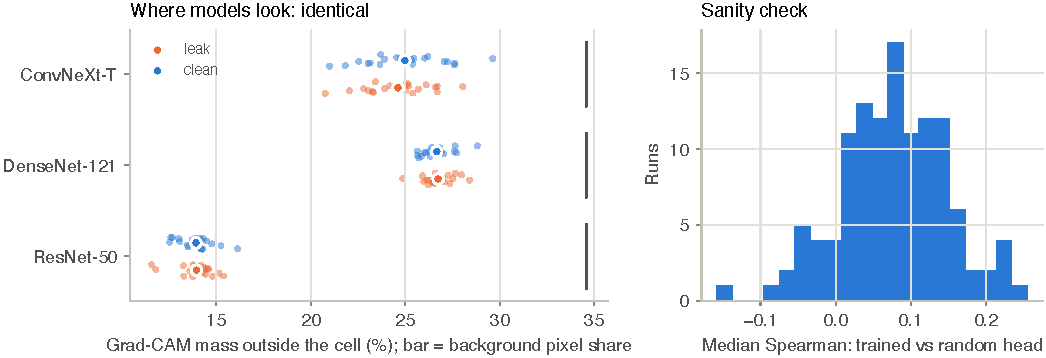
\includegraphics[width=\textwidth]{gradcam.pdf}
\caption{Left: per-run Grad-CAM attribution outside the cell for leak and clean models (bar: background pixel share).
Right: agreement of each run's maps with random-head maps.}
\label{r:fig:gradcam}
\end{figure}

{\footnotesize
\setlength{\tabcolsep}{3.5pt}
\begin{longtable}{llrrr}
\caption{Grad-CAM (descriptive): share of positive attribution outside the cell mask and background pixel share (percent, 20 runs each), and the median Spearman correlation with a random-head map.}\label{r:tab:gradcam}\\
\toprule
Architecture & Models & Attribution outside & Background pixels & Random-head $\rho$ \\
\midrule
\endfirsthead
\toprule
Architecture & Models & Attribution outside & Background pixels & Random-head $\rho$ \\
\midrule
\endhead
\bottomrule
\endfoot
ResNet-50 & leak & 13.9\,$\pm$\,1.0 & 34.6\,$\pm$\,0.5 & 0.085 \\
 & clean & 13.9\,$\pm$\,0.9 & 34.6\,$\pm$\,0.5 & 0.115 \\
DenseNet-121 & leak & 26.7\,$\pm$\,0.8 & 34.6\,$\pm$\,0.5 & 0.044 \\
 & clean & 26.7\,$\pm$\,0.8 & 34.6\,$\pm$\,0.5 & 0.057 \\
ConvNeXt-T & leak & 24.6\,$\pm$\,1.8 & 34.6\,$\pm$\,0.5 & 0.077 \\
 & clean & 25.0\,$\pm$\,2.2 & 34.6\,$\pm$\,0.5 & 0.076 \\
\end{longtable}
}


\chapter{The mechanism by elimination}
\label{r:ch:elimination}

\begin{figure}[H]
\centering
\begin{adjustbox}{max width=\textwidth}
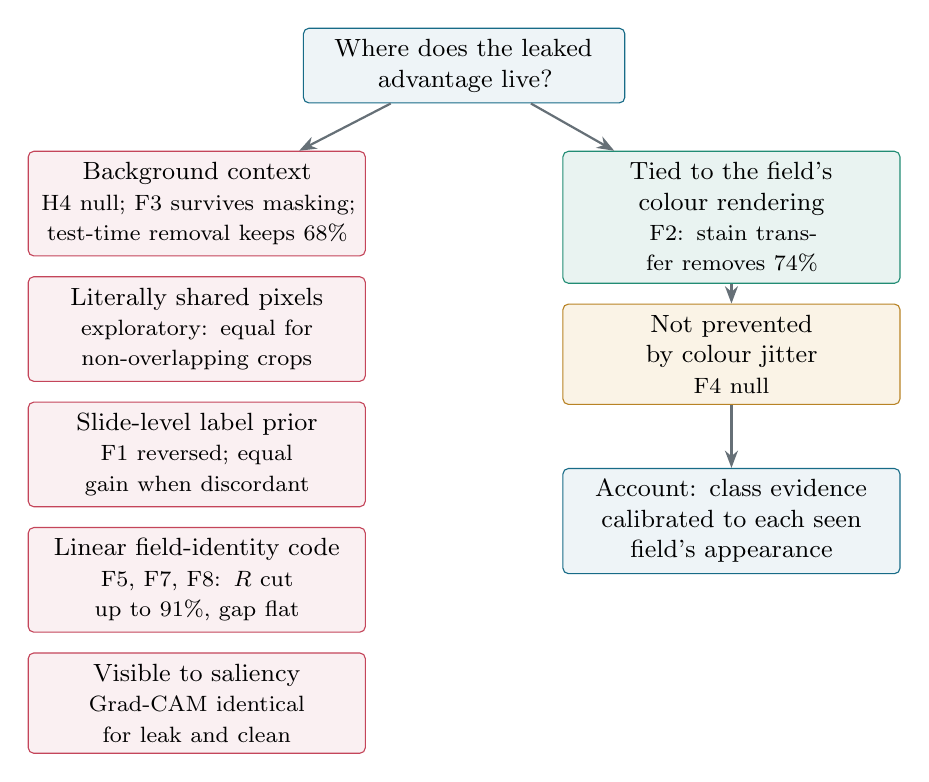
\begin{tikzpicture}[node distance=2.5mm and 6mm]
\node[box=38mm] (q) {Where does the leaked advantage live?};
\node[bad=40mm, below left=6mm and -8mm of q] (bg) {Background context\\\footnotesize H4 null; F3 survives masking; test-time removal keeps \RecBgKeep\%};
\node[bad=40mm, below=of bg] (pix) {Literally shared pixels\\\footnotesize exploratory: equal for non-overlapping crops};
\node[bad=40mm, below=of pix] (prior) {Slide-level label prior\\\footnotesize F1 reversed; equal gain when discordant};
\node[bad=40mm, below=of prior] (code) {Linear field-identity code\\\footnotesize F5, F7, F8: $R$ cut up to \RecoveryCutMax\%, gap flat};
\node[bad=40mm, below=of code] (sal) {Visible to saliency\\\footnotesize Grad-CAM identical for leak and clean};
\node[done=40mm, below right=6mm and -8mm of q] (colour) {Tied to the field's colour rendering\\\footnotesize F2: stain transfer removes \RecStainRemove\%};
\node[gold=40mm, below=of colour] (aug) {Not prevented by colour jitter\\\footnotesize F4 null};
\node[box=40mm, below=8mm of aug] (account) {Account: class evidence calibrated to each seen field's appearance};
\draw[flow] (q) -- (bg); \draw[flow] (q) -- (colour);
\draw[flow] (colour) -- (aug); \draw[flow] (aug) -- (account);
\end{tikzpicture}
\end{adjustbox}
\caption{The mechanism by elimination. Red: candidate carriers ruled out; green: the one intervention that removed most
of the advantage; gold: the qualification that keeps the account modest.}
\label{r:fig:elimination}
\end{figure}


Taken together with Study~2's H4 and H5, the follow-up narrows how models use the leak. The advantage does not need a
background (F3, test-time removal, H4). It is not memorisation of shared pixels (exploratory). It is not a slide-level label
prior (F1, reversed). It is not carried by a separable, linearly decodable field code: erasing that code in closed form, or
suppressing it with an adversary that cannot hide it from a linear probe, cut recoverability by \RecoveryCutMin--\RecoveryCutMax\%
without moving the gap (F5, F7, F8). What remains is that the advantage depends on the cell being rendered as its own field
renders cells: matching a test cell's colour statistics to another field of the same class removed most of it (F2).

The simplest account consistent with all of this is that a model trained on a field's siblings calibrates its class
evidence to that field's appearance (stain, colour balance, and the texture they produce in the cell itself), so cells
from a seen field sit further inside their class region. Random colour jitter during training did not prevent this (F4),
presumably because jitter perturbs each image around its own appearance and leaves the field-specific structure of that
appearance learnable. This account is a reading of the evidence, not a registered result, and the F2--F4 tension is the
part of it most in need of a direct test (for example, stain transfer applied to colour-augmented models).

\begin{decisionbox}{Decodable is not used, and saliency is not use}
Study~1 established \emph{availability}: a probe recognised fields at 109 times chance. The follow-up shows that availability
and use come apart: the identity a probe reads can be removed almost entirely without touching the inflation, in line with
evidence from language models that probe-decodable information need not be what a model relies
on~\citep{elazar2021amnesic,ravichander2021probing}. Grad-CAM showed leak and clean models attending to the same places; a
saliency audit would have cleared both.
\end{decisionbox}

\part{Synthesis}

\chapter{What the project established, refuted, and left open}
\label{r:ch:synthesis}

\section{Claims and their strength}

{\small
\begin{longtable}{p{0.30\textwidth}p{0.17\textwidth}p{0.45\textwidth}}
\caption{Every substantive claim of the project and how strongly the evidence supports it.}\label{r:tab:claims}\\
\toprule
Claim & Strength & Evidence and boundary \\
\midrule
\endfirsthead
\toprule
Claim & Strength & Evidence and boundary \\
\midrule
\endhead
\bottomrule
\endfoot
Public cytology benchmarks hide a crop-to-parent hierarchy & established & Study~1: recovered and verified for four datasets; Herlev negative control at zero. \\
Random crop splits share parents and pixels & established & 92.6\% (SIPaKMeD), 99.97\% (CRIC) of test cells with a training parent; \RecOverlapSip\% / \RecOverlapCric\% / \RecOverlapCx\% with shared pixels. \\
The parent is recognisable & established & Study~1 probe 109$\times$ chance; Study~2 encoder \RecEncoderTimes$\times$ chance. \\
Crop-level splitting inflates accuracy & established (registered, powered) & H1 +\HoneEst~pp, all twelve architectures; H2 +\HtwoEst~pp; five inference methods agree. \\
The inflation is leakage, not diversity & established (registered, replicated) & H3 +\HthreeEst~pp, diversity \DivEst~pp; replicated on fresh seeds (+\HthreeRepEst~pp). \\
Exposure follows structure & supported & CRIC, with 29 cells per slide and high class--slide dependence, inflates ten times more than SIPaKMeD; predicted by the closed forms. \\
The leak needs no background & established (registered) & F3 +\FthreeEst~pp with every background masked; test-time removal leaves \RecBgKeep\%. \\
The leak is tied to the field's colour rendering & supported (registered), qualified & F2 removes \RecStainRemove\% at test time; F4 shows colour jitter in training does not prevent it. \\
A background context route carries the leak & not supported & H4 \HfourEst~pp (\HfourLo\ to \HfourHi). \\
Models apply a slide-level label prior (CRIC) & refuted & F1 reversed (\FoneEst~pp); equal gains for discordant and concordant cells. \\
The leak is memorised shared pixels & not supported (exploratory) & Equal advantage on non-overlapping crops. \\
The inflation is carried by linearly decodable field identity & refuted within its scope & F5, F7, F8: recoverability cut \RecoveryCutMin--\RecoveryCutMax\%, gap flat (pooled slope \FeightEst, CI \FeightLo\ to \FeightHi). \\
Saliency maps reveal the leak & not supported (descriptive) & Grad-CAM identical for leak and clean models. \\
Stronger grouping (P3) is more conservative than P2 & not supported & P2 $-$ P3 \PtwoPthreeEst~pp; the ordering passes for \RecOrderingPassed\ of 12 architectures. \\
\end{longtable}
}

\section{What we got out of it}

\begin{workedbox}{Scientific results}
A certified, powered estimate of how much crop-level splitting inflates two public cytology benchmarks; a causal
separation of leakage from diversity; a mechanism narrowed by elimination; and a methodological warning that the
standard audit tools (probes, saliency, augmentation) cannot detect or remove this kind of leakage.
\end{workedbox}

\begin{workedbox}{Reusable artifacts}
Verified crop-to-parent maps for SIPaKMeD, Cx22, CRIC, and Herlev; registered P1/P1$'$/P2/P3 splits with hashes for 20
seeds; the 2C factorial designs and transplant plans; a risk calculator (\texttt{cytofair risk-report}) that predicts a
benchmark's exposure from its parent table; a deterministic GPU-resident training stack with complete per-run artifacts;
a fail-closed scheduler and collectors; exported records of every run (\artifact{results/study2/run_records}); 121~GB of
archived predictions, features, and weights for future analyses without retraining.
\end{workedbox}

\begin{workedbox}{Writing}
A single-column manuscript (\artifact{paper/v2}, 17 pages, every number generated), the earlier ISBI draft, the Study~1
record, and this lifecycle record.
\end{workedbox}

\chapter{What worked and what did not}
\label{r:ch:worked}

{\small
\begin{longtable}{p{0.18\textwidth}p{0.38\textwidth}p{0.36\textwidth}}
\caption{What worked and what did not, by area.}\label{r:tab:worked}\\
\toprule
Area & Worked & Did not work, or cost more than expected \\
\midrule
\endfirsthead
\toprule
Area & Worked & Did not work, or cost more than expected \\
\midrule
\endhead
\bottomrule
\endfoot
Question design & Separating structure, availability, consequence, and mechanism kept every claim at its true strength. & Study~1 asked the consequence question six times and could not answer it. \\
Statistics & One crossed mixed model with a split random effect, sized by simulation; registered sensitivity analyses that all agreed; the assumption trigger worked as designed. & Per-architecture testing in Study~1; Satterthwaite $df$ for H3 is only 3 with four architectures, so its interval is wide. \\
Causal designs & The 2C factorial cleanly separated leakage from diversity; evaluation-only follow-ups on saved models were cheap and decisive. & The 2B transplant contrast was noisy (sibling backgrounds help even clean models); the 2A MLP adversary was evaded by ConvNeXt-T. \\
Mechanism & Elimination with several independent manipulations gave a coherent picture. & No single test identifies the carrier positively; F2 and F4 pull in different directions. \\
Engineering & GPU-resident augmentation (exact torchvision port); packed hashed caches; bitwise determinism; complete per-run artifacts; zero failed tasks in 2,921. & The four-core CPU quota had to be discovered the hard way; the slow network home forced a strict storage discipline. \\
Governance & Register, smoke-test on non-contrast splits, dry-run, collect fail-closed, amend with dates; every deviation recorded. & A dry run that bypassed one pipeline stage let a labelling bug through to the first real analysis (Amendment~9). Registrations are local commits, not yet externally timestamped. \\
Operations & Detached controllers, status files, sequential offloading with verification, clean vacating of node-local storage. & Several shell and remote-wait mistakes (self-matching process searches, hung SSH sessions) cost time but no data. \\
\end{longtable}
}

\section{Demotivations, and why they mattered}

Four results were disappointing at the time. Study~1's six tests failed to survive correction, which looked like a null;
Study~2 showed it was underpowered. H4 and H5 failed to isolate a mechanism; Amendment~8 showed why (the leak is neither
in the background nor in a linearly readable code). F1 went the opposite way from the prediction; that reversal is itself
evidence against a slide-level label prior. And the ConvNeXt-T adversary was evaded; that failure is a concrete example
of why decodability and use must be measured separately. Each setback narrowed the explanation instead of ending it, and
none was hidden.

\section{Lessons}

\begin{enumerate}[leftmargin=1.8em]
\item Ask a pooled question once, with the dependence structure in the model (the shared test set per seed is a random
effect, not twelve independent tests).
\item Keep every per-sample artifact. Half of Amendment~8 cost no training because Study~2 kept logits, features, and
weights.
\item Measure manipulations independently of the mechanism they target: the gradient-reversal adversary's own accuracy
fell while an independent probe's rose.
\item Dry runs must pass through every stage of the real pipeline.
\item On shared hosts, discover the real resource limits (CPU quota, writable disks, network storage behaviour) before
designing the execution.
\end{enumerate}

\chapter{Decision log}
\label{r:ch:decisions}

Every design or execution decision that shaped a result, with the reason it was taken and the alternative it displaced.

{\small
\begin{longtable}{p{0.22\textwidth}p{0.40\textwidth}p{0.30\textwidth}}
\caption{Decisions and their reasons.}\label{r:tab:decisions}\\
\toprule
Decision & Reason & Alternative not taken \\
\midrule
\endfirsthead
\toprule
Decision & Reason & Alternative not taken \\
\midrule
\endhead
\bottomrule
\endfoot
\multicolumn{3}{l}{\textbf{Study 2 statistics}} \\
Add a split random effect to H1 & Twelve architectures share each seed's test set; without it the model treats twelve evaluations of one test set as independent. & The roadmap's formula without it. \\
Twenty seeds & Smallest count meeting the registered power rule (0.90 at pilot variances, 0.75 at 1.5$\times$). & 15 seeds (failed the inflated criterion); 25--30 (more compute for little power). \\
Twelve architectures & Breadth across CNNs, hierarchical transformers, plain ViTs, and a self-supervised model, so the effect is not tied to one family. & The six Study~1 models only. \\
Bootstrap primary when residuals are heavy-tailed & Registered before data; protects the primary test from non-normal seed-level noise. & Always the Satterthwaite $t$-test. \\
H2--H5 in one Holm family; H1 alone & H1 is the question; the mechanism tests are a family of related but separate claims. & One family of five (would have penalised the primary). \\
\multicolumn{3}{l}{\textbf{Study 2 designs}} \\
220 crops per class in 2C & Largest budget feasible for every registered seed and 100/100 unrelated seeds; 240 failed for seed 307. & 240 or 260 crops. \\
Common test set across all four 2C cells & Every cell is scored on the same crops, so differences are training effects only. & Separate test sets per cell. \\
Diversity estimated within clean cells only & The low-diversity leak cell gives each test crop more siblings, so the interaction confounds dose with diversity. & A full 2$\times$2 interpretation. \\
Sibling background as the 2B control & Isolates the cell's own acquisition context from class-typical context. & Only unseen-field backgrounds. \\
Class-conditional parent adversary & Suppressing parent identity must never require removing class information. & An unconditional 424-way adversary. \\
CRIC as $100\times100$ windows & CRIC releases nucleus coordinates on slide images, not crops; fixed windows are the simplest faithful crops. & Variable-size crops from annotations. \\
\multicolumn{3}{l}{\textbf{Execution}} \\
GPU-resident augmentation & Four-core CPU quota starved data loaders; an exact port keeps the registered recipe. & PIL augmentation in DataLoader workers. \\
One training job per GPU & GPUs were saturated by one job; two jobs shared throughput without speed-up. & Two jobs per GPU. \\
Math attention kernel only & Fused attention kernels have non-deterministic backward passes. & Faster fused kernels. \\
Float16 checkpoints & Halves storage of about 117~GB of weights; re-evaluation reproduces 418/480 models exactly, the rest within three crops. & Float32 checkpoints. \\
Amendment 7 before any 2A run & Deterministic divergence would otherwise have failed the whole arm. & Handling divergence after seeing it. \\
Registered analysis run on the GPU host & Run records point at node-local artifacts; moving gigabytes to a workstation was slower than computing in place. & Pulling all artifacts to the workstation. \\
\multicolumn{3}{l}{\textbf{Amendment 8}} \\
A separately registered follow-up & Study~2's mechanism tests were inconclusive, and saved artifacts made decisive tests cheap; registering first keeps them confirmatory for new questions. & Unregistered exploration, or re-testing H4/H5 with more seeds. \\
Reuse saved models where possible & F2 and F5 needed no training; three arms cost 7~GPU-hours in total. & Retraining for every arm. \\
Fresh seeds for retraining arms & New data for new questions; no reuse of Study~2 mechanism seeds. & Reusing the mechanism seeds. \\
Probe-matched linear adversary & ConvNeXt-T had evaded the MLP adversary; a standardised linear head cannot hide identity from a linear probe while leaving it readable. & Re-running the MLP adversary. \\
LEACE ranks up to 256 & The smallest feature dimension is 384 (DINOv2 ViT-S); 256 removes most within-class parent structure in every backbone. & Full-rank erasure (exceeds some feature dimensions). \\
HED-strong colour augmentation & A published, strong, stain-shaped perturbation. & Hue/saturation jitter only. \\
One device probe for every arm & Recoverability must be measured identically across manipulations; agreement with sklearn verified ($r=\ProbeAgreement$). & Mixing probe implementations. \\
Pixel-overlap split labelled exploratory & Added after the registered results to test a specific alternative explanation. & Presenting it as confirmatory. \\
\multicolumn{3}{l}{\textbf{Close-out}} \\
Offload checkpoints during the follow-up matrix & 52~GB of new checkpoints against a 71~GB margin; verified copies before deletion. & Pausing the matrix on the disk guard. \\
Recommend ISBI framing around audit tools & The registered evidence is strong; the novel take-home for an imaging audience is that probes and saliency cannot detect this leakage. & Framing around ``leakage exists''. \\
\end{longtable}
}

\chapter{Validity, recommendations, and next steps}
\label{r:ch:validity}

\section{Threats to validity}

\paragraph{Parents are not patients.} SIPaKMeD fields, Cx22 source images, and CRIC slide images are the deepest released
units. Several can come from one patient, so parent-disjoint evaluation is necessary but may not be sufficient for
clinical independence; every inflation estimate is a lower bound on what patient-level grouping would remove.

\paragraph{One recipe.} Every model used one fixed fine-tuning recipe. Stronger augmentation, longer training, or other
optimisers could change the size of the inflation and the models' reliance on acquisition context.

\paragraph{Smaller training sets in the factorial.} Matching crop and field counts required 220 crops per class (1,100 in
total against 3,239 in Phase~1); the 2C, 2B, and carrier effects are measured on smaller training sets than the headline
contrast, and the decomposition that transfers them is approximate.

\paragraph{Imperfect interventions.} Foreground masks are threshold rules; inpainting leaves smoothed backgrounds; Reinhard
transfer matches only first and second moments; erasure and adversaries act on pooled features and linear structure.

\paragraph{Post-results follow-up.} Amendment~8 was motivated by Study~2's results. Its hypotheses and analyses were fixed
before any follow-up run, but they are follow-up questions; the pixel-overlap split was added afterwards and is
exploratory.

\paragraph{CRIC crops.} The CRIC cells are windows cut by this project around published nucleus coordinates, not an
official crop release, so absolute CRIC accuracies are not directly comparable with published numbers.

\paragraph{External verification.} The registration commits have not yet been pushed or deposited; until they are, their
dates rest on the repository and on the commit hashes recorded inside every run.

\paragraph{No clinical claim.} The project audits research benchmarks; it does not estimate screening sensitivity,
specificity, prevalence-calibrated performance, or effects on readers.

\section{Recommendations}
\label{r:ch:recommendations}

\begin{enumerate}[leftmargin=1.8em]
\item \textbf{Release the hierarchy.} Every observation should carry its acquisition parent (field, source image, or slide),
a patient or specimen identifier where permitted, and, if audited, a duplicate-component identifier.
\item \textbf{Split at the deepest released unit and publish the split}, with its hash.
\item \textbf{Report both units}: observation and parent counts per split, and the fraction of test observations with a
training sibling.
\item \textbf{Check the structure before training} with the closed forms (\texttt{cytofair risk-report}).
\item \textbf{Treat one question as one test}, with a mixed model that treats architectures and splits as random effects,
sized by simulation.
\item \textbf{Do not certify a split with a probe, a saliency map, or an augmentation.} Leakage inflated accuracy with field
identity erased from the features, with identical Grad-CAM maps, with backgrounds removed, and with strong colour
augmentation.
\item \textbf{Keep the evidence}: per-sample predictions, final weights, and the exact split for every run.
\end{enumerate}

\section{Publication options and open decisions}
\label{r:ch:publication}

\subsection{Venues}
\label{r:sec:publication}

\paragraph{ISBI 2027.} Four pages including figures and tables (references may use a paid fifth page); deadline Monday 26
October 2026, 23:59 US Eastern; single-blind; arXiv preprints allowed; a ``Compliance with Ethical Standards'' section and a
disclosure of AI-generated content in the acknowledgments are required; presentation in person in Lausanne. The evidence is
stronger than typical for the venue. The risks are perceived novelty (patient-level splitting is textbook advice) and the
page limit. The recommended framing is ``how much crop-level splitting inflates public cytology benchmarks, and why the
usual audit tools cannot see it'': H1--H3 as the result, one figure (per-architecture SIPaKMeD with CRIC), one table of all
thirteen registered tests, and a paragraph on F2, F3, and the probe and Grad-CAM findings. Everything else waits for the
journal version.

\paragraph{Journal version.} The full manuscript (\artifact{paper/v2}) with Study~2 and Amendment~8. Check the journal's
policy on extended conference papers if ISBI is pursued first; ISBI only forbids simultaneous submission of a substantially
similar paper to another conference or workshop.

\paragraph{Preprint.} Allowed by ISBI; it would also give the registrations a public timestamp once the repository is pushed.

\subsection{Decisions only the authors can make}

\begin{itemize}[leftmargin=1.6em]
\item Push the \texttt{study2} branch (and the Cx22 commits) to the public repository, and deposit the preregistrations with
a third party (for example OSF) for an external timestamp.
\item Choose a software licence; confirm redistribution terms for derived artifacts (SIPaKMeD, CCEDD).
\item Co-author approval of every posted or submitted version; fill the e-mail and repository placeholders.
\item Whether to submit to ISBI 2027, and who presents in person.
\item The AI-use disclosure wording: much of the Study~2 code, analysis, manuscript text, and this record was drafted with
an AI assistant under the authors' direction.
\item Whether to open Phase~3 (other imaging domains) and the direct test of the F2--F4 tension.
\end{itemize}

\subsection{Future work}

\begin{itemize}[leftmargin=1.6em]
\item Apply test-time stain transfer to the colour-augmented carrier models to resolve the F2--F4 tension directly.
\item Non-linear and spatial (pre-pooling) erasure of field identity.
\item Patient-level grouping where a dataset's provenance allows it.
\item Other recipes (stronger augmentation, longer schedules, stain normalisation as standard practice).
\item Other domains where crops share acquisition units (the pre-specified fish-imagery V2).
\end{itemize}

\part{Appendices}
\appendix

\chapter*{About the appendices}
\addcontentsline{toc}{chapter}{About the appendices}
Appendices A--K are the Study~1 appendices, carried over verbatim. The remaining appendices hold the complete ledgers of
every Study~2 and Amendment~8 run, the variance components of every registered model, the commit chronology, the
registration hashes, the preregistration documents verbatim, and a reproduction cookbook.

% Carried over verbatim from monograph/main.tex (Study 1 record, 13 Sep 2026).
\chapter{Complete SIPaKMeD classifier run ledger}\label{s1:ch:app01_complete_sipakmed_classifier_run_ledger}

The following 120 rows are the entire accepted classifier matrix. Accuracy, macro-F1, and balanced accuracy are final-epoch test values. This appendix makes every seed visible and prevents mean-only reporting from hiding an outlying run.

\begin{landscape}
\footnotesize
\setlength{\tabcolsep}{3pt}
\begin{longtable}{p{2.25cm}p{1.1cm}rrrrrrrr}
\caption{Complete SIPaKMeD classification run ledger. All values are final-epoch results.}\label{s1:tab:all-class-runs}\\
\toprule
Architecture & Protocol & Seed & Train & Test & Acc. (percent) & Macro-F1 (percent) & Bal. acc. (percent) & min & GPU \\
\midrule
\endfirsthead
\toprule
Architecture & Protocol & Seed & Train & Test & Acc. (percent) & Macro-F1 (percent) & Bal. acc. (percent) & min & GPU \\
\midrule
\endhead
\bottomrule
\endfoot
densenet121 & P1 & 17 & 3239 & 810 & 98.519 & 98.521 & 98.527 & 4.66 & 3 \\ 
densenet121 & P1 & 29 & 3239 & 810 & 98.025 & 98.023 & 98.027 & 4.62 & 2 \\ 
densenet121 & P1 & 43 & 3239 & 810 & 97.778 & 97.776 & 97.803 & 4.54 & 1 \\ 
densenet121 & P1 & 71 & 3239 & 810 & 98.025 & 98.031 & 98.018 & 4.61 & 3 \\ 
densenet121 & P1 & 101 & 3239 & 810 & 98.272 & 98.284 & 98.276 & 4.70 & 2 \\ 
densenet121 & P1-prime & 17 & 3239 & 810 & 98.519 & 98.521 & 98.527 & 4.61 & 1 \\ 
densenet121 & P1-prime & 29 & 3239 & 810 & 98.025 & 98.023 & 98.027 & 4.48 & 3 \\ 
densenet121 & P1-prime & 43 & 3239 & 810 & 97.778 & 97.776 & 97.803 & 4.49 & 2 \\ 
densenet121 & P1-prime & 71 & 3239 & 810 & 98.025 & 98.031 & 98.018 & 4.48 & 1 \\ 
densenet121 & P1-prime & 101 & 3239 & 810 & 98.272 & 98.284 & 98.276 & 4.45 & 3 \\ 
densenet121 & P2 & 17 & 3239 & 810 & 95.926 & 95.972 & 95.946 & 4.47 & 2 \\ 
densenet121 & P2 & 29 & 3239 & 810 & 97.778 & 97.766 & 97.798 & 4.55 & 1 \\ 
densenet121 & P2 & 43 & 3239 & 810 & 96.914 & 96.927 & 96.906 & 4.51 & 3 \\ 
densenet121 & P2 & 71 & 3239 & 810 & 96.543 & 96.561 & 96.566 & 4.47 & 2 \\ 
densenet121 & P2 & 101 & 3239 & 810 & 96.420 & 96.446 & 96.395 & 4.59 & 1 \\ 
densenet121 & P3 & 17 & 3239 & 810 & 97.778 & 97.781 & 97.774 & 4.54 & 3 \\ 
densenet121 & P3 & 29 & 3239 & 810 & 97.901 & 97.895 & 97.904 & 4.64 & 2 \\ 
densenet121 & P3 & 43 & 3239 & 810 & 97.531 & 97.538 & 97.553 & 4.56 & 1 \\ 
densenet121 & P3 & 71 & 3239 & 810 & 96.790 & 96.824 & 96.801 & 4.20 & 3 \\ 
densenet121 & P3 & 101 & 3239 & 810 & 96.914 & 96.945 & 96.894 & 4.00 & 2 \\ 
efficientnet\_b0 & P1 & 17 & 3239 & 810 & 97.654 & 97.659 & 97.662 & 2.84 & 1 \\ 
efficientnet\_b0 & P1 & 29 & 3239 & 810 & 98.272 & 98.276 & 98.273 & 2.89 & 3 \\ 
efficientnet\_b0 & P1 & 43 & 3239 & 810 & 97.160 & 97.183 & 97.177 & 2.92 & 2 \\ 
efficientnet\_b0 & P1 & 71 & 3239 & 810 & 97.531 & 97.540 & 97.541 & 2.98 & 1 \\ 
efficientnet\_b0 & P1 & 101 & 3239 & 810 & 98.272 & 98.279 & 98.288 & 2.87 & 3 \\ 
efficientnet\_b0 & P1-prime & 17 & 3239 & 810 & 97.654 & 97.659 & 97.662 & 2.87 & 2 \\ 
efficientnet\_b0 & P1-prime & 29 & 3239 & 810 & 98.272 & 98.276 & 98.273 & 3.00 & 1 \\ 
efficientnet\_b0 & P1-prime & 43 & 3239 & 810 & 97.160 & 97.183 & 97.177 & 2.96 & 3 \\ 
efficientnet\_b0 & P1-prime & 71 & 3239 & 810 & 97.531 & 97.540 & 97.541 & 2.88 & 2 \\ 
efficientnet\_b0 & P1-prime & 101 & 3239 & 810 & 98.272 & 98.279 & 98.288 & 2.86 & 1 \\ 
efficientnet\_b0 & P2 & 17 & 3239 & 810 & 97.778 & 97.790 & 97.799 & 3.01 & 3 \\ 
efficientnet\_b0 & P2 & 29 & 3239 & 810 & 95.185 & 95.259 & 95.163 & 2.92 & 2 \\ 
efficientnet\_b0 & P2 & 43 & 3239 & 810 & 98.642 & 98.641 & 98.643 & 2.92 & 1 \\ 
efficientnet\_b0 & P2 & 71 & 3239 & 810 & 95.432 & 95.450 & 95.407 & 2.97 & 3 \\ 
efficientnet\_b0 & P2 & 101 & 3239 & 810 & 96.420 & 96.413 & 96.422 & 2.93 & 2 \\ 
efficientnet\_b0 & P3 & 17 & 3239 & 810 & 98.148 & 98.144 & 98.170 & 2.89 & 1 \\ 
efficientnet\_b0 & P3 & 29 & 3239 & 810 & 97.901 & 97.920 & 97.910 & 2.98 & 3 \\ 
efficientnet\_b0 & P3 & 43 & 3239 & 810 & 96.296 & 96.316 & 96.325 & 2.99 & 2 \\ 
efficientnet\_b0 & P3 & 71 & 3239 & 810 & 97.407 & 97.428 & 97.427 & 2.94 & 1 \\ 
efficientnet\_b0 & P3 & 101 & 3239 & 810 & 97.284 & 97.300 & 97.285 & 2.80 & 3 \\ 
mobilenet\_v2 & P1 & 17 & 3239 & 810 & 97.284 & 97.287 & 97.278 & 2.72 & 2 \\ 
mobilenet\_v2 & P1 & 29 & 3239 & 810 & 97.407 & 97.406 & 97.403 & 2.76 & 1 \\ 
mobilenet\_v2 & P1 & 43 & 3239 & 810 & 96.914 & 96.933 & 96.944 & 2.74 & 3 \\ 
mobilenet\_v2 & P1 & 71 & 3239 & 810 & 97.284 & 97.296 & 97.289 & 2.71 & 2 \\ 
mobilenet\_v2 & P1 & 101 & 3239 & 810 & 98.148 & 98.149 & 98.167 & 2.72 & 1 \\ 
mobilenet\_v2 & P1-prime & 17 & 3239 & 810 & 97.284 & 97.287 & 97.278 & 2.69 & 3 \\ 
mobilenet\_v2 & P1-prime & 29 & 3239 & 810 & 97.407 & 97.406 & 97.403 & 2.74 & 2 \\ 
mobilenet\_v2 & P1-prime & 43 & 3239 & 810 & 96.914 & 96.933 & 96.944 & 2.72 & 1 \\ 
mobilenet\_v2 & P1-prime & 71 & 3239 & 810 & 97.284 & 97.296 & 97.289 & 2.71 & 3 \\ 
mobilenet\_v2 & P1-prime & 101 & 3239 & 810 & 98.148 & 98.149 & 98.167 & 2.73 & 2 \\ 
mobilenet\_v2 & P2 & 17 & 3239 & 810 & 96.420 & 96.432 & 96.453 & 2.75 & 1 \\ 
mobilenet\_v2 & P2 & 29 & 3239 & 810 & 93.704 & 93.732 & 93.714 & 2.73 & 3 \\ 
mobilenet\_v2 & P2 & 43 & 3239 & 810 & 96.667 & 96.679 & 96.637 & 2.74 & 2 \\ 
mobilenet\_v2 & P2 & 71 & 3239 & 810 & 93.457 & 93.486 & 93.458 & 2.78 & 1 \\ 
mobilenet\_v2 & P2 & 101 & 3239 & 810 & 95.556 & 95.553 & 95.534 & 2.77 & 3 \\ 
mobilenet\_v2 & P3 & 17 & 3239 & 810 & 97.407 & 97.408 & 97.433 & 2.68 & 2 \\ 
mobilenet\_v2 & P3 & 29 & 3239 & 810 & 96.173 & 96.163 & 96.163 & 2.74 & 1 \\ 
mobilenet\_v2 & P3 & 43 & 3239 & 810 & 96.667 & 96.669 & 96.696 & 2.74 & 3 \\ 
mobilenet\_v2 & P3 & 71 & 3239 & 810 & 95.802 & 95.823 & 95.813 & 2.92 & 2 \\ 
mobilenet\_v2 & P3 & 101 & 3239 & 810 & 94.938 & 94.930 & 94.900 & 2.79 & 1 \\ 
resnet18 & P1 & 17 & 3239 & 810 & 97.901 & 97.900 & 97.930 & 2.57 & 1 \\ 
resnet18 & P1 & 29 & 3239 & 810 & 97.037 & 97.028 & 97.051 & 2.54 & 2 \\ 
resnet18 & P1 & 43 & 3239 & 810 & 96.914 & 96.922 & 96.938 & 2.48 & 3 \\ 
resnet18 & P1 & 71 & 3239 & 810 & 96.420 & 96.455 & 96.410 & 2.61 & 1 \\ 
resnet18 & P1 & 101 & 3239 & 810 & 97.654 & 97.661 & 97.674 & 2.54 & 2 \\ 
resnet18 & P1-prime & 17 & 3239 & 810 & 97.901 & 97.900 & 97.930 & 2.53 & 3 \\ 
resnet18 & P1-prime & 29 & 3239 & 810 & 97.037 & 97.028 & 97.051 & 2.62 & 1 \\ 
resnet18 & P1-prime & 43 & 3239 & 810 & 96.914 & 96.922 & 96.938 & 2.61 & 2 \\ 
resnet18 & P1-prime & 71 & 3239 & 810 & 96.420 & 96.455 & 96.410 & 2.48 & 3 \\ 
resnet18 & P1-prime & 101 & 3239 & 810 & 97.654 & 97.661 & 97.674 & 2.62 & 1 \\ 
resnet18 & P2 & 17 & 3239 & 810 & 96.420 & 96.444 & 96.447 & 2.58 & 2 \\ 
resnet18 & P2 & 29 & 3239 & 810 & 96.049 & 96.051 & 96.058 & 2.47 & 3 \\ 
resnet18 & P2 & 43 & 3239 & 810 & 96.543 & 96.535 & 96.502 & 2.49 & 1 \\ 
resnet18 & P2 & 71 & 3239 & 810 & 96.543 & 96.563 & 96.528 & 2.56 & 2 \\ 
resnet18 & P2 & 101 & 3239 & 810 & 94.444 & 94.436 & 94.384 & 2.50 & 3 \\ 
resnet18 & P3 & 17 & 3239 & 810 & 98.395 & 98.395 & 98.400 & 2.55 & 1 \\ 
resnet18 & P3 & 29 & 3239 & 810 & 95.062 & 95.069 & 95.014 & 2.55 & 3 \\ 
resnet18 & P3 & 43 & 3239 & 810 & 96.173 & 96.165 & 96.215 & 2.52 & 2 \\ 
resnet18 & P3 & 71 & 3239 & 810 & 96.543 & 96.578 & 96.561 & 2.79 & 1 \\ 
resnet18 & P3 & 101 & 3239 & 810 & 95.556 & 95.576 & 95.526 & 2.79 & 3 \\ 
resnet50 & P1 & 17 & 3239 & 810 & 97.778 & 97.781 & 97.792 & 3.73 & 2 \\ 
resnet50 & P1 & 29 & 3239 & 810 & 97.284 & 97.304 & 97.275 & 3.29 & 1 \\ 
resnet50 & P1 & 43 & 3239 & 810 & 96.790 & 96.801 & 96.805 & 3.32 & 3 \\ 
resnet50 & P1 & 71 & 3239 & 810 & 97.901 & 97.903 & 97.904 & 3.48 & 2 \\ 
resnet50 & P1 & 101 & 3239 & 810 & 97.778 & 97.776 & 97.777 & 3.45 & 1 \\ 
resnet50 & P1-prime & 17 & 3239 & 810 & 97.778 & 97.781 & 97.792 & 3.26 & 3 \\ 
resnet50 & P1-prime & 29 & 3239 & 810 & 97.284 & 97.304 & 97.275 & 3.45 & 2 \\ 
resnet50 & P1-prime & 43 & 3239 & 810 & 96.790 & 96.801 & 96.805 & 3.52 & 1 \\ 
resnet50 & P1-prime & 71 & 3239 & 810 & 97.901 & 97.903 & 97.904 & 3.34 & 3 \\ 
resnet50 & P1-prime & 101 & 3239 & 810 & 97.778 & 97.776 & 97.777 & 3.54 & 2 \\ 
resnet50 & P2 & 17 & 3239 & 810 & 97.037 & 97.067 & 97.053 & 3.47 & 1 \\ 
resnet50 & P2 & 29 & 3239 & 810 & 96.914 & 96.931 & 96.916 & 3.24 & 3 \\ 
resnet50 & P2 & 43 & 3239 & 810 & 97.284 & 97.298 & 97.290 & 3.45 & 2 \\ 
resnet50 & P2 & 71 & 3239 & 810 & 96.420 & 96.422 & 96.433 & 3.47 & 1 \\ 
resnet50 & P2 & 101 & 3239 & 810 & 96.296 & 96.303 & 96.288 & 3.29 & 3 \\ 
resnet50 & P3 & 17 & 3239 & 810 & 96.543 & 96.519 & 96.573 & 3.47 & 2 \\ 
resnet50 & P3 & 29 & 3239 & 810 & 97.037 & 97.071 & 97.049 & 3.46 & 1 \\ 
resnet50 & P3 & 43 & 3239 & 810 & 95.679 & 95.701 & 95.703 & 3.25 & 3 \\ 
resnet50 & P3 & 71 & 3239 & 810 & 95.926 & 95.945 & 95.958 & 3.73 & 2 \\ 
resnet50 & P3 & 101 & 3239 & 810 & 96.173 & 96.168 & 96.161 & 3.89 & 1 \\ 
vit\_b\_16 & P1 & 17 & 3239 & 810 & 97.407 & 97.414 & 97.430 & 9.30 & 3 \\ 
vit\_b\_16 & P1 & 29 & 3239 & 810 & 97.037 & 97.050 & 97.061 & 9.25 & 2 \\ 
vit\_b\_16 & P1 & 43 & 3239 & 810 & 95.556 & 95.541 & 95.606 & 9.35 & 1 \\ 
vit\_b\_16 & P1 & 71 & 3239 & 810 & 98.025 & 98.036 & 98.023 & 9.31 & 3 \\ 
vit\_b\_16 & P1 & 101 & 3239 & 810 & 97.654 & 97.666 & 97.684 & 9.27 & 2 \\ 
vit\_b\_16 & P1-prime & 17 & 3239 & 810 & 97.407 & 97.414 & 97.430 & 9.29 & 1 \\ 
vit\_b\_16 & P1-prime & 29 & 3239 & 810 & 97.037 & 97.050 & 97.061 & 9.19 & 3 \\ 
vit\_b\_16 & P1-prime & 43 & 3239 & 810 & 95.556 & 95.541 & 95.606 & 9.24 & 2 \\ 
vit\_b\_16 & P1-prime & 71 & 3239 & 810 & 98.025 & 98.036 & 98.023 & 9.30 & 1 \\ 
vit\_b\_16 & P1-prime & 101 & 3239 & 810 & 97.654 & 97.666 & 97.684 & 9.24 & 3 \\ 
vit\_b\_16 & P2 & 17 & 3239 & 810 & 95.556 & 95.618 & 95.526 & 9.27 & 2 \\ 
vit\_b\_16 & P2 & 29 & 3239 & 810 & 95.802 & 95.821 & 95.788 & 9.36 & 1 \\ 
vit\_b\_16 & P2 & 43 & 3239 & 810 & 96.667 & 96.693 & 96.688 & 9.32 & 3 \\ 
vit\_b\_16 & P2 & 71 & 3239 & 810 & 95.432 & 95.432 & 95.392 & 9.30 & 2 \\ 
vit\_b\_16 & P2 & 101 & 3239 & 810 & 94.321 & 94.421 & 94.283 & 9.28 & 1 \\ 
vit\_b\_16 & P3 & 17 & 3239 & 810 & 96.296 & 96.258 & 96.328 & 9.19 & 3 \\ 
vit\_b\_16 & P3 & 29 & 3239 & 810 & 95.185 & 95.218 & 95.214 & 9.23 & 2 \\ 
vit\_b\_16 & P3 & 43 & 3239 & 810 & 92.840 & 92.915 & 92.770 & 9.26 & 1 \\ 
vit\_b\_16 & P3 & 71 & 3239 & 810 & 97.284 & 97.292 & 97.301 & 9.00 & 3 \\ 
vit\_b\_16 & P3 & 101 & 3239 & 810 & 96.049 & 96.039 & 96.066 & 8.81 & 2 \\ 
\end{longtable}

\end{landscape}

% Carried over verbatim from monograph/main.tex (Study 1 record, 13 Sep 2026).
\chapter{Complete parent-probe run ledger}\label{s1:ch:app02_complete_parent_probe_run_ledger}

These 30 rows include five preprocessing arms and the label-shuffled negative control. All use exactly 424 parent classes, 848 training crops, and 848 held-out sibling crops.

\begin{landscape}
\footnotesize
\setlength{\tabcolsep}{3pt}
\begin{longtable}{p{2.4cm}p{1.0cm}rrrrrrrr}
\caption{Complete parent-identity probe ledger.}\label{s1:tab:all-probe-runs}\\
\toprule
Mode & Shuffle & Seed & Parents & Train & Test & Chance (percent) & Accuracy (percent) & min & GPU \\
\midrule
\endfirsthead
\toprule
Mode & Shuffle & Seed & Parents & Train & Test & Chance (percent) & Accuracy (percent) & min & GPU \\
\midrule
\endhead
\bottomrule
\endfoot
background\_only & no & 17 & 424 & 848 & 848 & 0.2358 & 18.514 & 21.00 & 3 \\ 
background\_only & no & 29 & 424 & 848 & 848 & 0.2358 & 20.047 & 20.55 & 1 \\ 
background\_only & no & 43 & 424 & 848 & 848 & 0.2358 & 19.811 & 20.23 & 2 \\ 
background\_only & no & 71 & 424 & 848 & 848 & 0.2358 & 17.925 & 89.59 & 3 \\ 
background\_only & no & 101 & 424 & 848 & 848 & 0.2358 & 17.099 & 89.40 & 2 \\ 
grayscale & no & 17 & 424 & 848 & 848 & 0.2358 & 15.212 & 0.93 & 3 \\ 
grayscale & no & 29 & 424 & 848 & 848 & 0.2358 & 13.208 & 0.88 & 2 \\ 
grayscale & no & 43 & 424 & 848 & 848 & 0.2358 & 14.741 & 1.02 & 1 \\ 
grayscale & no & 71 & 424 & 848 & 848 & 0.2358 & 13.208 & 0.97 & 2 \\ 
grayscale & no & 101 & 424 & 848 & 848 & 0.2358 & 12.618 & 1.02 & 3 \\ 
highpass & no & 17 & 424 & 848 & 848 & 0.2358 & 16.863 & 15.73 & 1 \\ 
highpass & no & 29 & 424 & 848 & 848 & 0.2358 & 16.156 & 15.87 & 1 \\ 
highpass & no & 43 & 424 & 848 & 848 & 0.2358 & 16.863 & 15.93 & 1 \\ 
highpass & no & 71 & 424 & 848 & 848 & 0.2358 & 16.038 & 15.80 & 1 \\ 
highpass & no & 101 & 424 & 848 & 848 & 0.2358 & 15.448 & 16.04 & 1 \\ 
rgb & no & 17 & 424 & 848 & 848 & 0.2358 & 25.943 & 0.89 & 1 \\ 
rgb & no & 29 & 424 & 848 & 848 & 0.2358 & 26.769 & 0.76 & 2 \\ 
rgb & no & 43 & 424 & 848 & 848 & 0.2358 & 25.236 & 0.76 & 3 \\ 
rgb & no & 71 & 424 & 848 & 848 & 0.2358 & 25.590 & 0.77 & 1 \\ 
rgb & no & 101 & 424 & 848 & 848 & 0.2358 & 25.118 & 0.79 & 2 \\ 
rgb & yes & 17 & 424 & 848 & 848 & 0.2358 & 0.590 & 0.78 & 3 \\ 
rgb & yes & 29 & 424 & 848 & 848 & 0.2358 & 0.000 & 0.88 & 1 \\ 
rgb & yes & 43 & 424 & 848 & 848 & 0.2358 & 0.118 & 0.86 & 3 \\ 
rgb & yes & 71 & 424 & 848 & 848 & 0.2358 & 0.000 & 0.76 & 2 \\ 
rgb & yes & 101 & 424 & 848 & 848 & 0.2358 & 0.118 & 0.82 & 1 \\ 
stain\_normalized & no & 17 & 424 & 848 & 848 & 0.2358 & 17.335 & 2.49 & 1 \\ 
stain\_normalized & no & 29 & 424 & 848 & 848 & 0.2358 & 17.099 & 2.41 & 2 \\ 
stain\_normalized & no & 43 & 424 & 848 & 848 & 0.2358 & 18.396 & 2.26 & 3 \\ 
stain\_normalized & no & 71 & 424 & 848 & 848 & 0.2358 & 16.745 & 2.42 & 1 \\ 
stain\_normalized & no & 101 & 424 & 848 & 848 & 0.2358 & 16.981 & 2.20 & 2 \\ 
\end{longtable}

\end{landscape}

% Carried over verbatim from monograph/main.tex (Study 1 record, 13 Sep 2026).
\chapter{Complete Cx22 model run ledger}\label{s1:ch:app03_complete_cx22_model_run_ledger}

The following 175 rows are all accepted Cx22 cells: five semantic architectures and two instance architectures, each under five protocols and five seeds. ``Primary'' is semantic macro-Dice or matched-instance Dice; ``Nuc./R70'' is nucleus Dice for semantic rows and Recall@0.70 for instance rows.

\begin{landscape}
\scriptsize
\setlength{\tabcolsep}{2.2pt}
\begin{longtable}{p{1.6cm}p{4.4cm}p{1.5cm}rrrrrrr}
\caption{Complete Cx22 run ledger. Primary is macro Dice for semantic models and matched-instance Dice for instance models; the ninth column is nucleus Dice or recall at Dice 0.70.}\label{s1:tab:all-cx22-runs}\\
\toprule
Task & Architecture & Protocol & Seed & Train & Test & Primary (percent) & IoU (percent) & Nuc./R70 (percent) & hours \\
\midrule
\endfirsthead
\toprule
Task & Architecture & Protocol & Seed & Train & Test & Primary (percent) & IoU (percent) & Nuc./R70 (percent) & hours \\
\midrule
\endhead
\bottomrule
\endfoot
instance & \path{maskrcnn_resnet50_fpn} & OFFICIAL & 17 & 400 & 100 & 92.117 & 87.060 & 96.991 & 14.35 \\ 
instance & \path{maskrcnn_resnet50_fpn} & OFFICIAL & 29 & 400 & 100 & 92.372 & 87.354 & 97.068 & 14.92 \\ 
instance & \path{maskrcnn_resnet50_fpn} & OFFICIAL & 43 & 400 & 100 & 91.844 & 86.861 & 96.682 & 15.89 \\ 
instance & \path{maskrcnn_resnet50_fpn} & OFFICIAL & 71 & 400 & 100 & 92.669 & 87.541 & 97.608 & 0.49 \\ 
instance & \path{maskrcnn_resnet50_fpn} & OFFICIAL & 101 & 400 & 100 & 92.433 & 87.559 & 97.145 & 1.29 \\ 
instance & \path{maskrcnn_resnet50_fpn} & P1 & 17 & 1056 & 264 & 92.683 & 87.370 & 96.540 & 33.85 \\ 
instance & \path{maskrcnn_resnet50_fpn} & P1 & 29 & 1056 & 264 & 91.354 & 86.327 & 95.009 & 33.71 \\ 
instance & \path{maskrcnn_resnet50_fpn} & P1 & 43 & 1056 & 264 & 92.282 & 87.191 & 96.854 & 35.84 \\ 
instance & \path{maskrcnn_resnet50_fpn} & P1 & 71 & 1056 & 264 & 92.343 & 87.320 & 96.550 & 37.54 \\ 
instance & \path{maskrcnn_resnet50_fpn} & P1 & 101 & 1056 & 264 & 91.819 & 86.735 & 96.471 & 2.55 \\ 
instance & \path{maskrcnn_resnet50_fpn} & P1-prime & 17 & 1056 & 264 & 92.683 & 87.370 & 96.540 & 33.94 \\ 
instance & \path{maskrcnn_resnet50_fpn} & P1-prime & 29 & 1056 & 264 & 91.354 & 86.327 & 95.009 & 33.95 \\ 
instance & \path{maskrcnn_resnet50_fpn} & P1-prime & 43 & 1056 & 264 & 92.282 & 87.191 & 96.854 & 35.19 \\ 
instance & \path{maskrcnn_resnet50_fpn} & P1-prime & 71 & 1055 & 264 & 91.733 & 86.958 & 95.483 & 38.29 \\ 
instance & \path{maskrcnn_resnet50_fpn} & P1-prime & 101 & 1053 & 264 & 92.213 & 87.257 & 97.248 & 2.56 \\ 
instance & \path{maskrcnn_resnet50_fpn} & P2 & 17 & 1056 & 264 & 91.815 & 86.503 & 95.983 & 33.84 \\ 
instance & \path{maskrcnn_resnet50_fpn} & P2 & 29 & 1056 & 264 & 91.313 & 86.228 & 95.159 & 34.29 \\ 
instance & \path{maskrcnn_resnet50_fpn} & P2 & 43 & 1056 & 264 & 92.024 & 86.559 & 96.750 & 35.88 \\ 
instance & \path{maskrcnn_resnet50_fpn} & P2 & 71 & 1055 & 265 & 90.993 & 85.998 & 92.239 & 0.26 \\ 
instance & \path{maskrcnn_resnet50_fpn} & P2 & 101 & 1053 & 267 & 91.793 & 86.639 & 94.671 & 2.57 \\ 
instance & \path{maskrcnn_resnet50_fpn} & P3 & 17 & 891 & 429 & 89.855 & 84.435 & 94.937 & 47.44 \\ 
instance & \path{maskrcnn_resnet50_fpn} & P3 & 29 & 825 & 495 & 91.606 & 86.357 & 95.207 & 49.79 \\ 
instance & \path{maskrcnn_resnet50_fpn} & P3 & 43 & 894 & 426 & 90.023 & 84.807 & 94.415 & 47.25 \\ 
instance & \path{maskrcnn_resnet50_fpn} & P3 & 71 & 773 & 547 & 92.181 & 86.751 & 96.205 & 1.16 \\ 
instance & \path{maskrcnn_resnet50_fpn} & P3 & 101 & 791 & 529 & 91.910 & 86.399 & 96.806 & 1.98 \\ 
instance & \path{maskrcnn_resnet50_fpn_v2} & OFFICIAL & 17 & 400 & 100 & 91.970 & 87.274 & 95.910 & 1.31 \\ 
instance & \path{maskrcnn_resnet50_fpn_v2} & OFFICIAL & 29 & 400 & 100 & 92.548 & 87.588 & 96.991 & 1.33 \\ 
instance & \path{maskrcnn_resnet50_fpn_v2} & OFFICIAL & 43 & 400 & 100 & 91.041 & 86.290 & 94.367 & 1.32 \\ 
instance & \path{maskrcnn_resnet50_fpn_v2} & OFFICIAL & 71 & 400 & 100 & 92.442 & 87.459 & 97.068 & 1.69 \\ 
instance & \path{maskrcnn_resnet50_fpn_v2} & OFFICIAL & 101 & 400 & 100 & 92.886 & 87.943 & 97.531 & 1.40 \\ 
instance & \path{maskrcnn_resnet50_fpn_v2} & P1 & 17 & 1056 & 264 & 91.235 & 86.322 & 91.816 & 2.63 \\ 
instance & \path{maskrcnn_resnet50_fpn_v2} & P1 & 29 & 1056 & 264 & 91.543 & 86.726 & 92.276 & 2.64 \\ 
instance & \path{maskrcnn_resnet50_fpn_v2} & P1 & 43 & 1056 & 264 & 92.536 & 87.688 & 94.870 & 2.65 \\ 
instance & \path{maskrcnn_resnet50_fpn_v2} & P1 & 71 & 1056 & 264 & 92.342 & 87.566 & 94.856 & 2.63 \\ 
instance & \path{maskrcnn_resnet50_fpn_v2} & P1 & 101 & 1056 & 264 & 92.318 & 87.546 & 95.131 & 2.99 \\ 
instance & \path{maskrcnn_resnet50_fpn_v2} & P1-prime & 17 & 1056 & 264 & 91.235 & 86.322 & 91.816 & 2.63 \\ 
instance & \path{maskrcnn_resnet50_fpn_v2} & P1-prime & 29 & 1056 & 264 & 91.543 & 86.726 & 92.276 & 2.63 \\ 
instance & \path{maskrcnn_resnet50_fpn_v2} & P1-prime & 43 & 1056 & 264 & 92.536 & 87.688 & 94.870 & 2.64 \\ 
instance & \path{maskrcnn_resnet50_fpn_v2} & P1-prime & 71 & 1055 & 264 & 91.938 & 87.241 & 93.915 & 2.62 \\ 
instance & \path{maskrcnn_resnet50_fpn_v2} & P1-prime & 101 & 1053 & 264 & 92.502 & 87.584 & 95.272 & 2.85 \\ 
instance & \path{maskrcnn_resnet50_fpn_v2} & P2 & 17 & 1056 & 264 & 92.036 & 87.121 & 95.303 & 2.64 \\ 
instance & \path{maskrcnn_resnet50_fpn_v2} & P2 & 29 & 1056 & 264 & 91.737 & 86.754 & 94.870 & 2.65 \\ 
instance & \path{maskrcnn_resnet50_fpn_v2} & P2 & 43 & 1056 & 264 & 92.056 & 86.980 & 95.297 & 2.65 \\ 
instance & \path{maskrcnn_resnet50_fpn_v2} & P2 & 71 & 1055 & 265 & 90.232 & 85.363 & 87.492 & 2.64 \\ 
instance & \path{maskrcnn_resnet50_fpn_v2} & P2 & 101 & 1053 & 267 & 90.762 & 85.672 & 92.038 & 2.70 \\ 
instance & \path{maskrcnn_resnet50_fpn_v2} & P3 & 17 & 891 & 429 & 91.242 & 85.867 & 94.762 & 2.26 \\ 
instance & \path{maskrcnn_resnet50_fpn_v2} & P3 & 29 & 825 & 495 & 89.960 & 84.956 & 91.273 & 2.10 \\ 
instance & \path{maskrcnn_resnet50_fpn_v2} & P3 & 43 & 894 & 426 & 90.317 & 85.094 & 91.622 & 2.29 \\ 
instance & \path{maskrcnn_resnet50_fpn_v2} & P3 & 71 & 773 & 547 & 90.474 & 85.440 & 90.769 & 1.98 \\ 
instance & \path{maskrcnn_resnet50_fpn_v2} & P3 & 101 & 791 & 529 & 91.026 & 85.770 & 94.358 & 2.02 \\ 
semantic & \path{deeplabv3plus_resnet50} & OFFICIAL & 17 & 400 & 100 & 82.697 & 72.771 & 71.084 & 1.02 \\ 
semantic & \path{deeplabv3plus_resnet50} & OFFICIAL & 29 & 400 & 100 & 83.602 & 73.897 & 72.700 & 1.13 \\ 
semantic & \path{deeplabv3plus_resnet50} & OFFICIAL & 43 & 400 & 100 & 84.126 & 74.580 & 73.775 & 1.08 \\ 
semantic & \path{deeplabv3plus_resnet50} & OFFICIAL & 71 & 400 & 100 & 83.972 & 74.385 & 73.418 & 1.12 \\ 
semantic & \path{deeplabv3plus_resnet50} & OFFICIAL & 101 & 400 & 100 & 80.382 & 70.180 & 66.995 & 1.11 \\ 
semantic & \path{deeplabv3plus_resnet50} & P1 & 17 & 1056 & 264 & 88.570 & 80.909 & 81.412 & 2.09 \\ 
semantic & \path{deeplabv3plus_resnet50} & P1 & 29 & 1056 & 264 & 88.464 & 80.728 & 81.373 & 1.91 \\ 
semantic & \path{deeplabv3plus_resnet50} & P1 & 43 & 1056 & 264 & 89.196 & 81.695 & 82.572 & 2.02 \\ 
semantic & \path{deeplabv3plus_resnet50} & P1 & 71 & 1056 & 264 & 89.542 & 82.165 & 83.162 & 2.14 \\ 
semantic & \path{deeplabv3plus_resnet50} & P1 & 101 & 1056 & 264 & 88.738 & 81.195 & 81.662 & 2.32 \\ 
semantic & \path{deeplabv3plus_resnet50} & P1-prime & 17 & 1056 & 264 & 88.570 & 80.909 & 81.412 & 2.13 \\ 
semantic & \path{deeplabv3plus_resnet50} & P1-prime & 29 & 1056 & 264 & 88.464 & 80.728 & 81.373 & 1.93 \\ 
semantic & \path{deeplabv3plus_resnet50} & P1-prime & 43 & 1056 & 264 & 89.196 & 81.695 & 82.572 & 2.03 \\ 
semantic & \path{deeplabv3plus_resnet50} & P1-prime & 71 & 1055 & 264 & 89.443 & 82.040 & 82.958 & 2.14 \\ 
semantic & \path{deeplabv3plus_resnet50} & P1-prime & 101 & 1053 & 264 & 88.514 & 80.848 & 81.162 & 2.28 \\ 
semantic & \path{deeplabv3plus_resnet50} & P2 & 17 & 1056 & 264 & 88.304 & 80.549 & 81.070 & 1.90 \\ 
semantic & \path{deeplabv3plus_resnet50} & P2 & 29 & 1056 & 264 & 88.930 & 81.407 & 82.016 & 2.03 \\ 
semantic & \path{deeplabv3plus_resnet50} & P2 & 43 & 1056 & 264 & 88.731 & 80.967 & 81.799 & 1.99 \\ 
semantic & \path{deeplabv3plus_resnet50} & P2 & 71 & 1055 & 265 & 88.988 & 81.513 & 82.202 & 2.22 \\ 
semantic & \path{deeplabv3plus_resnet50} & P2 & 101 & 1053 & 267 & 88.268 & 80.470 & 80.952 & 2.28 \\ 
semantic & \path{deeplabv3plus_resnet50} & P3 & 17 & 891 & 429 & 88.332 & 80.528 & 81.111 & 2.13 \\ 
semantic & \path{deeplabv3plus_resnet50} & P3 & 29 & 825 & 495 & 87.707 & 79.682 & 80.088 & 2.57 \\ 
semantic & \path{deeplabv3plus_resnet50} & P3 & 43 & 894 & 426 & 88.621 & 80.940 & 81.705 & 2.70 \\ 
semantic & \path{deeplabv3plus_resnet50} & P3 & 71 & 773 & 547 & 88.041 & 80.050 & 80.594 & 3.46 \\ 
semantic & \path{deeplabv3plus_resnet50} & P3 & 101 & 791 & 529 & 87.790 & 79.677 & 80.185 & 3.43 \\ 
semantic & \path{fpn_resnet34} & OFFICIAL & 17 & 400 & 100 & 84.378 & 74.779 & 74.746 & 1.08 \\ 
semantic & \path{fpn_resnet34} & OFFICIAL & 29 & 400 & 100 & 84.801 & 75.377 & 75.422 & 1.12 \\ 
semantic & \path{fpn_resnet34} & OFFICIAL & 43 & 400 & 100 & 84.389 & 74.760 & 74.723 & 1.10 \\ 
semantic & \path{fpn_resnet34} & OFFICIAL & 71 & 400 & 100 & 84.630 & 75.136 & 75.152 & 1.07 \\ 
semantic & \path{fpn_resnet34} & OFFICIAL & 101 & 400 & 100 & 83.934 & 74.231 & 73.850 & 1.09 \\ 
semantic & \path{fpn_resnet34} & P1 & 17 & 1056 & 264 & 88.606 & 80.936 & 81.657 & 2.30 \\ 
semantic & \path{fpn_resnet34} & P1 & 29 & 1056 & 264 & 88.376 & 80.651 & 81.204 & 2.17 \\ 
semantic & \path{fpn_resnet34} & P1 & 43 & 1056 & 264 & 89.242 & 81.731 & 82.802 & 2.29 \\ 
semantic & \path{fpn_resnet34} & P1 & 71 & 1056 & 264 & 89.415 & 81.991 & 83.139 & 2.29 \\ 
semantic & \path{fpn_resnet34} & P1 & 101 & 1056 & 264 & 88.854 & 81.286 & 81.903 & 2.31 \\ 
semantic & \path{fpn_resnet34} & P1-prime & 17 & 1056 & 264 & 88.606 & 80.936 & 81.657 & 2.23 \\ 
semantic & \path{fpn_resnet34} & P1-prime & 29 & 1056 & 264 & 88.376 & 80.651 & 81.204 & 2.19 \\ 
semantic & \path{fpn_resnet34} & P1-prime & 43 & 1056 & 264 & 89.242 & 81.731 & 82.802 & 2.30 \\ 
semantic & \path{fpn_resnet34} & P1-prime & 71 & 1055 & 264 & 89.760 & 82.473 & 83.695 & 2.30 \\ 
semantic & \path{fpn_resnet34} & P1-prime & 101 & 1053 & 264 & 88.880 & 81.350 & 81.891 & 2.26 \\ 
semantic & \path{fpn_resnet34} & P2 & 17 & 1056 & 264 & 88.539 & 80.901 & 81.452 & 2.18 \\ 
semantic & \path{fpn_resnet34} & P2 & 29 & 1056 & 264 & 89.006 & 81.470 & 82.385 & 2.20 \\ 
semantic & \path{fpn_resnet34} & P2 & 43 & 1056 & 264 & 89.498 & 82.080 & 83.321 & 2.22 \\ 
semantic & \path{fpn_resnet34} & P2 & 71 & 1055 & 265 & 89.102 & 81.618 & 82.649 & 2.24 \\ 
semantic & \path{fpn_resnet34} & P2 & 101 & 1053 & 267 & 88.296 & 80.471 & 81.211 & 2.25 \\ 
semantic & \path{fpn_resnet34} & P3 & 17 & 891 & 429 & 88.029 & 80.133 & 80.698 & 2.84 \\ 
semantic & \path{fpn_resnet34} & P3 & 29 & 825 & 495 & 88.080 & 80.127 & 80.967 & 3.16 \\ 
semantic & \path{fpn_resnet34} & P3 & 43 & 894 & 426 & 88.744 & 81.048 & 82.174 & 2.75 \\ 
semantic & \path{fpn_resnet34} & P3 & 71 & 773 & 547 & 88.510 & 80.711 & 81.583 & 3.46 \\ 
semantic & \path{fpn_resnet34} & P3 & 101 & 791 & 529 & 88.287 & 80.367 & 81.266 & 3.45 \\ 
semantic & \path{manet_resnet34} & OFFICIAL & 17 & 400 & 100 & 83.189 & 73.517 & 71.864 & 1.06 \\ 
semantic & \path{manet_resnet34} & OFFICIAL & 29 & 400 & 100 & 86.409 & 77.571 & 77.856 & 1.08 \\ 
semantic & \path{manet_resnet34} & OFFICIAL & 43 & 400 & 100 & 86.521 & 77.608 & 78.266 & 1.07 \\ 
semantic & \path{manet_resnet34} & OFFICIAL & 71 & 400 & 100 & 86.256 & 77.306 & 77.825 & 1.15 \\ 
semantic & \path{manet_resnet34} & OFFICIAL & 101 & 400 & 100 & 85.118 & 75.878 & 75.519 & 1.19 \\ 
semantic & \path{manet_resnet34} & P1 & 17 & 1056 & 264 & 89.317 & 81.998 & 82.837 & 2.13 \\ 
semantic & \path{manet_resnet34} & P1 & 29 & 1056 & 264 & 89.510 & 82.294 & 83.125 & 2.19 \\ 
semantic & \path{manet_resnet34} & P1 & 43 & 1056 & 264 & 90.535 & 83.620 & 85.003 & 2.09 \\ 
semantic & \path{manet_resnet34} & P1 & 71 & 1056 & 264 & 90.674 & 83.752 & 85.088 & 2.06 \\ 
semantic & \path{manet_resnet34} & P1 & 101 & 1056 & 264 & 90.128 & 83.049 & 84.158 & 2.14 \\ 
semantic & \path{manet_resnet34} & P1-prime & 17 & 1056 & 264 & 89.317 & 81.998 & 82.837 & 2.17 \\ 
semantic & \path{manet_resnet34} & P1-prime & 29 & 1056 & 264 & 89.510 & 82.294 & 83.125 & 2.06 \\ 
semantic & \path{manet_resnet34} & P1-prime & 43 & 1056 & 264 & 90.535 & 83.620 & 85.003 & 2.05 \\ 
semantic & \path{manet_resnet34} & P1-prime & 71 & 1055 & 264 & 90.764 & 83.957 & 85.467 & 2.05 \\ 
semantic & \path{manet_resnet34} & P1-prime & 101 & 1053 & 264 & 90.221 & 83.230 & 84.212 & 2.07 \\ 
semantic & \path{manet_resnet34} & P2 & 17 & 1056 & 264 & 89.337 & 81.962 & 83.086 & 2.14 \\ 
semantic & \path{manet_resnet34} & P2 & 29 & 1056 & 264 & 90.185 & 83.160 & 84.409 & 2.08 \\ 
semantic & \path{manet_resnet34} & P2 & 43 & 1056 & 264 & 90.170 & 83.032 & 84.460 & 2.01 \\ 
semantic & \path{manet_resnet34} & P2 & 71 & 1055 & 265 & 90.458 & 83.608 & 84.919 & 2.09 \\ 
semantic & \path{manet_resnet34} & P2 & 101 & 1053 & 267 & 89.687 & 82.410 & 83.599 & 2.00 \\ 
semantic & \path{manet_resnet34} & P3 & 17 & 891 & 429 & 89.762 & 82.615 & 83.748 & 2.75 \\ 
semantic & \path{manet_resnet34} & P3 & 29 & 825 & 495 & 89.392 & 82.029 & 83.305 & 2.62 \\ 
semantic & \path{manet_resnet34} & P3 & 43 & 894 & 426 & 89.895 & 82.761 & 83.970 & 2.16 \\ 
semantic & \path{manet_resnet34} & P3 & 71 & 773 & 547 & 89.469 & 82.176 & 83.199 & 3.03 \\ 
semantic & \path{manet_resnet34} & P3 & 101 & 791 & 529 & 89.625 & 82.349 & 83.609 & 1.96 \\ 
semantic & \path{unet_resnet34} & OFFICIAL & 17 & 400 & 100 & 85.332 & 76.145 & 75.734 & 1.03 \\ 
semantic & \path{unet_resnet34} & OFFICIAL & 29 & 400 & 100 & 85.420 & 76.382 & 75.839 & 1.11 \\ 
semantic & \path{unet_resnet34} & OFFICIAL & 43 & 400 & 100 & 85.102 & 75.810 & 75.351 & 1.03 \\ 
semantic & \path{unet_resnet34} & OFFICIAL & 71 & 400 & 100 & 86.580 & 77.740 & 78.197 & 1.13 \\ 
semantic & \path{unet_resnet34} & OFFICIAL & 101 & 400 & 100 & 85.749 & 76.664 & 76.744 & 1.06 \\ 
semantic & \path{unet_resnet34} & P1 & 17 & 1056 & 264 & 90.196 & 83.235 & 84.389 & 2.09 \\ 
semantic & \path{unet_resnet34} & P1 & 29 & 1056 & 264 & 89.654 & 82.414 & 83.452 & 2.16 \\ 
semantic & \path{unet_resnet34} & P1 & 43 & 1056 & 264 & 90.616 & 83.797 & 85.081 & 2.01 \\ 
semantic & \path{unet_resnet34} & P1 & 71 & 1056 & 264 & 90.880 & 84.082 & 85.657 & 2.09 \\ 
semantic & \path{unet_resnet34} & P1 & 101 & 1056 & 264 & 90.093 & 82.967 & 84.100 & 2.04 \\ 
semantic & \path{unet_resnet34} & P1-prime & 17 & 1056 & 264 & 90.196 & 83.235 & 84.389 & 2.12 \\ 
semantic & \path{unet_resnet34} & P1-prime & 29 & 1056 & 264 & 89.654 & 82.414 & 83.452 & 2.20 \\ 
semantic & \path{unet_resnet34} & P1-prime & 43 & 1056 & 264 & 90.616 & 83.797 & 85.081 & 1.98 \\ 
semantic & \path{unet_resnet34} & P1-prime & 71 & 1055 & 264 & 91.020 & 84.317 & 85.849 & 2.06 \\ 
semantic & \path{unet_resnet34} & P1-prime & 101 & 1053 & 264 & 90.092 & 83.064 & 84.113 & 1.95 \\ 
semantic & \path{unet_resnet34} & P2 & 17 & 1056 & 264 & 89.429 & 82.217 & 83.000 & 2.10 \\ 
semantic & \path{unet_resnet34} & P2 & 29 & 1056 & 264 & 90.249 & 83.272 & 84.602 & 2.17 \\ 
semantic & \path{unet_resnet34} & P2 & 43 & 1056 & 264 & 90.674 & 83.773 & 85.275 & 2.03 \\ 
semantic & \path{unet_resnet34} & P2 & 71 & 1055 & 265 & 89.519 & 82.235 & 83.280 & 2.16 \\ 
semantic & \path{unet_resnet34} & P2 & 101 & 1053 & 267 & 90.082 & 82.951 & 84.446 & 2.01 \\ 
semantic & \path{unet_resnet34} & P3 & 17 & 891 & 429 & 89.911 & 82.788 & 83.948 & 2.23 \\ 
semantic & \path{unet_resnet34} & P3 & 29 & 825 & 495 & 89.629 & 82.392 & 83.516 & 2.85 \\ 
semantic & \path{unet_resnet34} & P3 & 43 & 894 & 426 & 89.892 & 82.748 & 83.984 & 2.82 \\ 
semantic & \path{unet_resnet34} & P3 & 71 & 773 & 547 & 89.840 & 82.694 & 83.704 & 3.12 \\ 
semantic & \path{unet_resnet34} & P3 & 101 & 791 & 529 & 89.576 & 82.274 & 83.557 & 2.96 \\ 
semantic & \path{unetplusplus_resnet34} & OFFICIAL & 17 & 400 & 100 & 85.933 & 77.036 & 76.615 & 1.06 \\ 
semantic & \path{unetplusplus_resnet34} & OFFICIAL & 29 & 400 & 100 & 86.864 & 78.288 & 78.526 & 1.15 \\ 
semantic & \path{unetplusplus_resnet34} & OFFICIAL & 43 & 400 & 100 & 86.771 & 78.140 & 78.396 & 1.11 \\ 
semantic & \path{unetplusplus_resnet34} & OFFICIAL & 71 & 400 & 100 & 88.276 & 79.991 & 81.686 & 1.08 \\ 
semantic & \path{unetplusplus_resnet34} & OFFICIAL & 101 & 400 & 100 & 88.645 & 80.557 & 82.123 & 1.08 \\ 
semantic & \path{unetplusplus_resnet34} & P1 & 17 & 1056 & 264 & 90.270 & 83.391 & 84.440 & 1.97 \\ 
semantic & \path{unetplusplus_resnet34} & P1 & 29 & 1056 & 264 & 89.890 & 82.832 & 83.858 & 1.88 \\ 
semantic & \path{unetplusplus_resnet34} & P1 & 43 & 1056 & 264 & 90.909 & 84.191 & 85.525 & 2.05 \\ 
semantic & \path{unetplusplus_resnet34} & P1 & 71 & 1056 & 264 & 91.190 & 84.587 & 86.038 & 1.89 \\ 
semantic & \path{unetplusplus_resnet34} & P1 & 101 & 1056 & 264 & 90.564 & 83.715 & 84.868 & 2.26 \\ 
semantic & \path{unetplusplus_resnet34} & P1-prime & 17 & 1056 & 264 & 90.270 & 83.391 & 84.440 & 1.97 \\ 
semantic & \path{unetplusplus_resnet34} & P1-prime & 29 & 1056 & 264 & 89.890 & 82.832 & 83.858 & 1.85 \\ 
semantic & \path{unetplusplus_resnet34} & P1-prime & 43 & 1056 & 264 & 90.909 & 84.191 & 85.525 & 2.03 \\ 
semantic & \path{unetplusplus_resnet34} & P1-prime & 71 & 1055 & 264 & 91.266 & 84.711 & 86.229 & 1.85 \\ 
semantic & \path{unetplusplus_resnet34} & P1-prime & 101 & 1053 & 264 & 90.576 & 83.692 & 84.939 & 2.27 \\ 
semantic & \path{unetplusplus_resnet34} & P2 & 17 & 1056 & 264 & 90.077 & 83.064 & 84.058 & 1.87 \\ 
semantic & \path{unetplusplus_resnet34} & P2 & 29 & 1056 & 264 & 90.324 & 83.431 & 84.639 & 1.91 \\ 
semantic & \path{unetplusplus_resnet34} & P2 & 43 & 1056 & 264 & 90.205 & 83.068 & 84.221 & 2.03 \\ 
semantic & \path{unetplusplus_resnet34} & P2 & 71 & 1055 & 265 & 90.977 & 84.343 & 85.735 & 1.81 \\ 
semantic & \path{unetplusplus_resnet34} & P2 & 101 & 1053 & 267 & 90.300 & 83.261 & 84.697 & 2.02 \\ 
semantic & \path{unetplusplus_resnet34} & P3 & 17 & 891 & 429 & 90.011 & 82.987 & 84.055 & 2.10 \\ 
semantic & \path{unetplusplus_resnet34} & P3 & 29 & 825 & 495 & 89.719 & 82.531 & 83.578 & 2.58 \\ 
semantic & \path{unetplusplus_resnet34} & P3 & 43 & 894 & 426 & 90.126 & 83.176 & 84.281 & 2.19 \\ 
semantic & \path{unetplusplus_resnet34} & P3 & 71 & 773 & 547 & 90.283 & 83.365 & 84.578 & 2.56 \\ 
semantic & \path{unetplusplus_resnet34} & P3 & 101 & 791 & 529 & 90.099 & 83.076 & 84.302 & 2.83 \\ 
\end{longtable}

\end{landscape}

% Carried over verbatim from monograph/main.tex (Study 1 record, 13 Sep 2026).
\chapter{Owner data files and integrity hashes}\label{s1:ch:app04_owner_data_files_and_integrity_hashes}

This table is generated from \artifact{data_sources.json}. A reproduction refuses a file whose byte length or SHA-256 differs, even if its archive name is unchanged.

\begin{landscape}
\scriptsize
\setlength{\tabcolsep}{3pt}
\begin{longtable}{p{1.5cm}p{3.5cm}rp{8.0cm}p{9.0cm}}
\caption{Declared owner-source files, exact byte sizes, checksums, and use notes.}\label{s1:tab:data-sources}\\
\toprule
Dataset & File & Bytes & SHA-256 & Terms note \\
\midrule
\endfirsthead
\toprule
Dataset & File & Bytes & SHA-256 & Terms note \\
\midrule
\endhead
\bottomrule
\endfoot
sipakmed & im\_Superficial-Intermediate.7z & 762,939,737 & \seqsplit{3b73e406df14d60b1bd9c8ac3b01b594e70bb51ba32fb080141fc6a7f489a599} & Public for experimental use; cite Plissiti et al., ICIP 2018 \\ 
sipakmed & im\_Parabasal.7z & 548,667,699 & \seqsplit{13e9c29f016a5b83731e038cfe518671a7815df28836dee706acba6ecd2369a8} & Public for experimental use; cite Plissiti et al., ICIP 2018 \\ 
sipakmed & im\_Koilocytotic.7z & 1,290,478,065 & \seqsplit{653578e878e3cc63a8510cd7ec26d918637d9881e913e29a5bb205d0d9cfb70d} & Public for experimental use; cite Plissiti et al., ICIP 2018 \\ 
sipakmed & im\_Metaplastic.7z & 1,396,480,123 & \seqsplit{97f1badc5f606f127d2af0d18a008ebd41a2b60f44785cb332a6eaa33004d2af} & Public for experimental use; cite Plissiti et al., ICIP 2018 \\ 
sipakmed & im\_Dyskeratotic.7z & 1,182,980,549 & \seqsplit{a8768bc03c9e814063ff946b7ef7548067e16b760168267d2b12e95a66955cce} & Public for experimental use; cite Plissiti et al., ICIP 2018 \\ 
cx22 & Cx22-Multi-Test.zip & 1,780,461 & \seqsplit{6d444e6e4bf8734073bc90e6e2bb29b0e36c66f7b783cbad9f969208621624bb} & Non-commercial research and education only \\ 
cx22 & Cx22-Multi-Train.zip & 6,361,959 & \seqsplit{171be9caf6d0709f3fce2b81a07e1974229c5faae355f197efe553ec1d6d1992} & Non-commercial research and education only \\ 
cx22 & Cx22-Pair.zip & 3,705,743 & \seqsplit{130b6a92db9811151a60e27dc70f4180965ecf0f1dbc84146c87d00c41d7ba9f} & Non-commercial research and education only \\ 
ccedd & CCEDD.zip & 1,507,832,267 & \seqsplit{d85e6a380a15923f0c2b38e13dd31467f75d11b49e8d21740f16ee69082cdcb1} & Non-commercial research and education only; redistribution prohibited \\ 
cric & classifications.csv & 1,224,400 & \seqsplit{e1f50183998ddb7392d2a0d4c96dce44c00dbe3833df03f266cc36e047445de5} & CC BY 4.0; cite Rezende et al. and the Figshare record \\ 
herlev & Cervical Cell Image Database.zip & 44,688,829 & \seqsplit{5b5b740abb599710b9d97fe72954540df9ca7255b2b40a52c8b25ac90d0c50da} & CC BY 4.0; repackaging of the original Herlev cervical-cell images \\ 
\end{longtable}

\end{landscape}

% Carried over verbatim from monograph/main.tex (Study 1 record, 13 Sep 2026).
\chapter{Released split hashes}\label{s1:ch:app05_released_split_hashes}

Each CSV contains crop ID, parent ID, partition, protocol, and seed. Hashes identify the exact semantic assignment rather than merely naming a random seed.

{\scriptsize
\setlength{\tabcolsep}{3pt}
\begin{longtable}{p{1.5cm}rp{4.8cm}p{6.4cm}}
\caption{Released SIPaKMeD split manifests and hashes.}\label{s1:tab:split-hashes}\\
\toprule
Protocol & Seed & File & SHA-256 \\
\midrule
\endfirsthead
\toprule
Protocol & Seed & File & SHA-256 \\
\midrule
\endhead
\bottomrule
\endfoot
P1 & 17 & sipakmed\_p1\_seed17.csv & \seqsplit{28abd1605d72d888f561cecbc4d987b0dafff671653c37d0460bccac8d3c0cac} \\ 
P1-prime & 17 & sipakmed\_p1\_prime\_seed17.csv & \seqsplit{611fcb7e6ed98e66a86f9cbdbcb27644850e15d93a4143249dc611d00364d784} \\ 
P2 & 17 & sipakmed\_p2\_seed17.csv & \seqsplit{488077976eb9397b2a772597e4453e2a31e809d67cb1a21595ece5b143b35262} \\ 
P3 & 17 & sipakmed\_p3\_seed17.csv & \seqsplit{797a4c0d73fd0722aebec95a14cf798ac3cf94575ac7e93812a85b738df0ea14} \\ 
P1 & 29 & sipakmed\_p1\_seed29.csv & \seqsplit{adef646d2edabf02bf92a00a7a8e68eefee876159ee2d43d1ab4c25fc80e1e75} \\ 
P1-prime & 29 & sipakmed\_p1\_prime\_seed29.csv & \seqsplit{72f36aa2713e5dbd4a7d16f471ec466f88dacefbf597d5831bf3b409cc9cb256} \\ 
P2 & 29 & sipakmed\_p2\_seed29.csv & \seqsplit{4088e6c4b03fca9e16ecb7db57b221e1769e09a5bf6f9c2f36b52519332aed21} \\ 
P3 & 29 & sipakmed\_p3\_seed29.csv & \seqsplit{3722ec8802c1bbfdf4fe7d9aad2ecd99be4ca66da83add1e331f6d816ed936cc} \\ 
P1 & 43 & sipakmed\_p1\_seed43.csv & \seqsplit{d5087a1636cceebd8943accfbeb2129046772df01276a693b202f02340846beb} \\ 
P1-prime & 43 & sipakmed\_p1\_prime\_seed43.csv & \seqsplit{a7417cb3eeccbc4629bd212afffc2c3f42045e9d864f10b232b2c1f15e3a4b1b} \\ 
P2 & 43 & sipakmed\_p2\_seed43.csv & \seqsplit{bd1a079eadacd51adbeb0dc169d0bcca5cf3b011d3d6b71bb98e4fa71988a62f} \\ 
P3 & 43 & sipakmed\_p3\_seed43.csv & \seqsplit{877f62465214f160aaa2776bd4ba92c2054c78d744261ae9ada9a4ce66343de8} \\ 
P1 & 71 & sipakmed\_p1\_seed71.csv & \seqsplit{5148ddbc11d90a927f6cf7d9bc5213d0b1431b9d80cb58fa0d870de76c889198} \\ 
P1-prime & 71 & sipakmed\_p1\_prime\_seed71.csv & \seqsplit{21ce3cab719badee5dad0bb192c2e55e695fe44d35d58c0a9c6921e4aa7c5b3a} \\ 
P2 & 71 & sipakmed\_p2\_seed71.csv & \seqsplit{52095a0a39a27f439d64646ed50b07f15bfc729dee195a42f0dcb4c4739d0e25} \\ 
P3 & 71 & sipakmed\_p3\_seed71.csv & \seqsplit{bbf975f39f790159dcc903bb3d53eb87968e6d612066bfe0cd5c1e8fb6cc860e} \\ 
P1 & 101 & sipakmed\_p1\_seed101.csv & \seqsplit{1dadec3ecdbce04080b796d735ca7ecfe84cc4b74342d8480326b7c95dd9ff44} \\ 
P1-prime & 101 & sipakmed\_p1\_prime\_seed101.csv & \seqsplit{d9e096b00642b40eb979f3d75e827f6929e15d0c62a3a9a3738eb4490526185f} \\ 
P2 & 101 & sipakmed\_p2\_seed101.csv & \seqsplit{178418b059a5c924b305ca5a05472b2076f3423626538e27416ad39f6e1f891f} \\ 
P3 & 101 & sipakmed\_p3\_seed101.csv & \seqsplit{269ac8e1badbad7c11a5a45cd72b2c2d17ac0fa2c09cb0fa007b45ce51bbef90} \\ 
\end{longtable}

}

% Carried over verbatim from monograph/main.tex (Study 1 record, 13 Sep 2026).
\chapter{Git decision chronology}\label{s1:ch:app06_git_decision_chronology}

The chronology below is descriptive provenance for major decisions and corrections. The authoritative ordering remains the Git object database. In particular, the first entry is the original preregistration commit.

{\scriptsize
\setlength{\tabcolsep}{3pt}
\begin{longtable}{p{1.5cm}p{2.0cm}p{11.5cm}}
\caption{Complete repository decision chronology through the frozen result set.}\label{s1:tab:git-timeline}\\
\toprule
Commit & Date & Recorded change \\
\midrule
\endfirsthead
\toprule
Commit & Date & Recorded change \\
\midrule
\endhead
\bottomrule
\endfoot
67e8ded & 2026-08-22 & preregister confirmatory analysis \\ 
8ebc6d5 & 2026-08-22 & build leakage verification pipeline \\ 
12c9de7 & 2026-08-22 & add parent identity probe and complete source checksums \\ 
4ba6a96 & 2026-08-22 & make image provenance recovery independent \\ 
1dbd6ac & 2026-08-22 & separate provenance recovery stages \\ 
c551f2d & 2026-08-22 & add matched classification harness \\ 
14a1569 & 2026-08-22 & add near duplicate audit and P3 grouping \\ 
79b798a & 2026-08-22 & amend SIPaKMeD class order before analysis \\ 
70b5ffa & 2026-08-22 & add bounded GPU probe launcher \\ 
4aa3e60 & 2026-08-22 & fail closed on image provenance confidence \\ 
c18d393 & 2026-08-22 & validate Cx22 against declared source images \\ 
f7ca331 & 2026-08-22 & add bounded matched evaluation launcher \\ 
318120f & 2026-08-22 & summarize matched runs in one correction family \\ 
8f6f76e & 2026-08-22 & complete preregistered probe ablations \\ 
680fa53 & 2026-08-22 & record reproducible model run metadata \\ 
0c5166e & 2026-08-22 & checkpoint exhaustive provenance matching \\ 
ea053e9 & 2026-08-22 & verify structural protocol ordering \\ 
65b0230 & 2026-08-22 & export fixed protocol split assets \\ 
3261dc0 & 2026-08-22 & render fail-closed verification contract \\ 
79e5b31 & 2026-08-22 & require named provenance evidence in report \\ 
cded044 & 2026-08-22 & measure literal cross-split pixel overlap \\ 
55708d4 & 2026-08-22 & keep training commands free of analysis-only imports \\ 
6369698 & 2026-08-22 & generate self-contained thesis figure \\ 
da548a4 & 2026-08-22 & bound clean reproduction matcher to three workers \\ 
83d56af & 2026-08-22 & verify published class crop counts \\ 
03e7442 & 2026-08-22 & document fail-closed release workflow \\ 
be46a53 & 2026-08-22 & separate canonical and audit provenance maps \\ 
c617374 & 2026-08-22 & bound provenance image cache to class working set \\ 
4c6282e & 2026-08-22 & use multiscale provenance matching only as fallback \\ 
67892b7 & 2026-08-22 & align provenance validation with registered criteria \\ 
268e56a & 2026-08-22 & build explicit section 11 acceptance ledger \\ 
438fa3f & 2026-08-22 & measure duplicate detector precision and recall \\ 
62a51ef & 2026-08-22 & record virgin-host reproduction evidence \\ 
dd0a56e & 2026-08-22 & generate five-seed parent probe figure \\ 
b90805a & 2026-08-22 & reproduce P3 splits and pixel overlap end to end \\ 
82e541d & 2026-08-22 & add matched protocol results figure \\ 
adf5539 & 2026-08-22 & document full matched classifier matrix \\ 
bf8a4ec & 2026-08-22 & enforce paper table reporting contract \\ 
ab40681 & 2026-08-22 & separate Figure 2 control labels \\ 
a72fb5f & 2026-08-22 & record split and image library versions \\ 
4da9f62 & 2026-08-22 & pin CUDA 12.8 training environment \\ 
f936802 & 2026-08-22 & verify classification matrix integrity \\ 
157b882 & 2026-08-22 & report secondary ordering violations \\ 
10fb2a3 & 2026-08-22 & pin reproducible split runtime \\ 
970c74e & 2026-08-22 & gate acceptance on matrix integrity \\ 
8ebb2b9 & 2026-08-22 & simulate exact P1 allocation rule \\ 
525df1d & 2026-08-22 & report architecture ranking stability \\ 
1c2da7f & 2026-08-22 & record preregistered provenance and five-seed results \\ 
2c5d5c3 & 2026-08-22 & record post-result acceptance evidence \\ 
d347b07 & 2026-08-24 & preregister Cx22 segmentation rescore \\ 
a58f72f & 2026-08-24 & add resumable Cx22 segmentation extension \\ 
635e660 & 2026-08-24 & decode Cx22 instance labels with bounded memory \\ 
2fdb136 & 2026-08-24 & refresh Cx22 controller heartbeat during epochs \\ 
d66dba4 & 2026-08-24 & add memory-mapped Cx22 training cache \\ 
a18ddef & 2026-08-24 & preregister mixed-precision Cx22 execution \\ 
f10c9c5 & 2026-08-24 & enable preregistered mixed precision for Cx22 \\ 
48c9b65 & 2026-08-28 & stabilize Cx22 MAnet training in FP32 \\ 
373276a & 2026-08-28 & enforce deterministic CUDA workspace for Cx22 \\ 
a9594b3 & 2026-09-06 & remove redundant Cx22 instance runtime overhead \\ 
01c4c31 & 2026-09-06 & stage Cx22 checkpoints off network storage \\ 
\end{longtable}

}

% Carried over verbatim from monograph/main.tex (Study 1 record, 13 Sep 2026).
\chapter{Exact command cookbook}\label{s1:ch:app07_exact_command_cookbook}

\section{Local checks}

\begin{lstlisting}[style=cyto,language=bash]
uv sync --extra dev
uv run pytest
uv run ruff check .
uv run cytofair --help
\end{lstlisting}

\section{Recover and verify structural evidence}

\begin{lstlisting}[style=cyto,language=bash]
uv run cytofair recover-sipakmed data/extracted/sipakmed --workers 3
uv run cytofair recover-cx22 data/extracted/cx22 \
  --image-root data/extracted/ccedd/png
uv run cytofair recover-cric data/raw/cric/classifications.csv
uv run cytofair recover-herlev data/extracted/herlev

uv run cytofair audit-duplicates \
  provenance/sipakmed_parent_map.parquet \
  --hashes results/duplicates/sipakmed_hashes.parquet \
  --pairs results/duplicates/sipakmed_near_duplicate_pairs.csv \
  --output provenance/sipakmed_parent_map_p3.parquet

uv run cytofair make-splits \
  provenance/sipakmed_parent_map_p3.parquet \
  --dataset SIPaKMeD --output splits/generated

uv run cytofair pixel-overlap \
  provenance/sipakmed_branch_b.parquet --dataset SIPaKMeD
\end{lstlisting}

\section{Launch the probe and classifier matrices}

\begin{lstlisting}[style=cyto,language=bash]
python scripts/launch_probe_matrix.py \
  provenance/sipakmed_parent_map_p3.parquet results/probe \
  --max-gpus 3 \
  --modes rgb grayscale stain_normalized background_only highpass

python scripts/launch_classification_matrix.py \
  --dataset-map SIPaKMeD=provenance/sipakmed_parent_map_p3.parquet \
  --output results/classification --max-gpus 3 \
  --architectures resnet18 resnet50 densenet121 \
    efficientnet_b0 mobilenet_v2 vit_b_16 \
  --protocols P1 P1-prime P2 P3
\end{lstlisting}

\section{Materialize and launch Cx22}

\begin{lstlisting}[style=cyto,language=bash]
cytofair materialize-cx22 provenance/cx22_parent_map.parquet \
  --labels /path/to/extracted/cx22 \
  --assets /path/to/cx22_assets \
  --output provenance/cx22_model_map.parquet

cytofair audit-duplicates provenance/cx22_model_map.parquet \
  --hashes results/cx22_duplicates/hashes.parquet \
  --pairs results/cx22_duplicates/pairs.csv \
  --output provenance/cx22_model_map_p3.parquet

cytofair cache-cx22 provenance/cx22_model_map_p3.parquet \
  --cache /path/to/cx22_assets/cache256 \
  --output provenance/cx22_cached_model_map_p3.parquet

nohup python scripts/launch_cx22_segmentation_matrix.py \
  --map provenance/cx22_cached_model_map_p3.parquet \
  --output results/cx22_segmentation --max-gpus 3 \
  > results/cx22_segmentation/controller.log 2>&1 < /dev/null &

python scripts/check_cx22_segmentation.py results/cx22_segmentation
\end{lstlisting}

% Carried over verbatim from monograph/main.tex (Study 1 record, 13 Sep 2026).
\chapter{Artifact index and evidence status}\label{s1:ch:app08_artifact_index_and_evidence_status}

\begin{longtable}{p{0.29\textwidth}p{0.20\textwidth}p{0.43\textwidth}}
\caption{Principal repository artifacts.}
\label{s1:tab:artifacts}\\
\toprule
Artifact & Status & Purpose \\
\midrule
\endfirsthead
\toprule
Artifact & Status & Purpose \\
\midrule
\endhead
\bottomrule
\endfoot
\artifact{PREREGISTRATION.md} & Frozen plan & Endpoints, seeds, protocols, exclusions, corrections, amendments. \\
\artifact{data_sources.json} & Versioned & Owner URLs, filenames, sizes, hashes, and terms notes. \\
\artifact{provenance/*.parquet} & Complete derived maps & Observation-to-parent identities, match diagnostics, boxes, hashes, and P3 components. \\
\artifact{splits/*.csv} & Versioned interface & Exact per-seed assignments joined by crop ID. \\
\artifact{results/classification/*.json} & 120 accepted & Classifier metrics, environment, split hash, and history. \\
\artifact{results/probe/*.json} & 30 accepted & Mechanism probe metrics, chance, environment, and history. \\
\artifact{results/cx22_segmentation/*.json} & 175 accepted & Semantic/instance metrics, manifests, runtime, and history. \\
\artifact{results/attempts/} & Excluded, retained & Twelve incompatible split-library runs and three smoke tests. \\
\artifact{reports/generated/acceptance_contract.*} & Current & Machine-readable PASS/FAIL/PENDING gates. \\
\artifact{scripts/reproduce_table1.sh} & Implemented & GPU-free raw-download-to-structural-table workflow. \\
\artifact{scripts/verify_clean_clone.sh} & Implemented, unattested & Non-local clone wrapper and optional virgin-host attestation. \\
\artifact{reports/lab_paper_self_audit.md} & Pending & Nine-record title/protocol crosswalk requiring source-paper checks. \\
\artifact{reports/figure1_reader_test.md} & Pending & Independent reader protocol and blank response record. \\
\end{longtable}

% Carried over verbatim from monograph/main.tex (Study 1 record, 13 Sep 2026).
\chapter{Complete derived-result ledgers}\label{s1:ch:app09_complete_derived_result_ledgers}

These tables expose every structural seed, literal-overlap seed/protocol, registered classifier contrast, registered Cx22 contrast, and rank-stability result. The model run ledgers in Appendices A--C are the underlying run-level evidence; this appendix is the complete derived statistical layer.

\section{Structural and literal-overlap seeds}

{\small
\setlength{\tabcolsep}{3pt}
\begin{longtable}{p{2.0cm}p{1.0cm}p{2.5cm}p{2.8cm}p{2.5cm}p{2.5cm}}
\caption{Complete structural seed ledger.}\label{s1:tab:structural-seed-ledger}\\
\toprule
Dataset & Seed & P1 parent straddle (percent) & P1 test parent in train (percent) & P2 straddle (percent) & P3 straddle (percent) \\
\midrule
\endfirsthead
\toprule
Dataset & Seed & P1 parent straddle (percent) & P1 test parent in train (percent) & P2 straddle (percent) & P3 straddle (percent) \\
\midrule
\endhead
\bottomrule
\endfoot
SIPaKMeD & 17 & 45.549 & 92.222 & 0.000 & 0.000 \\ 
SIPaKMeD & 29 & 45.445 & 92.840 & 0.000 & 0.000 \\ 
SIPaKMeD & 43 & 44.203 & 92.469 & 0.000 & 0.000 \\ 
SIPaKMeD & 71 & 47.101 & 93.210 & 0.000 & 0.000 \\ 
SIPaKMeD & 101 & 45.859 & 92.346 & 0.000 & 0.000 \\ 
Cx22 & 17 & 34.241 & 85.985 & 0.000 & 0.000 \\ 
Cx22 & 29 & 32.685 & 80.682 & 0.000 & 0.000 \\ 
Cx22 & 43 & 35.214 & 89.773 & 0.000 & 0.000 \\ 
Cx22 & 71 & 34.825 & 86.742 & 0.000 & 0.000 \\ 
Cx22 & 101 & 33.074 & 82.955 & 0.000 & 0.000 \\ 
CRIC & 17 & 94.750 & 99.827 & 0.000 & 0.000 \\ 
CRIC & 29 & 95.000 & 100.000 & 0.000 & 0.000 \\ 
CRIC & 43 & 94.250 & 100.000 & 0.000 & 0.000 \\ 
CRIC & 71 & 92.500 & 100.000 & 0.000 & 0.000 \\ 
CRIC & 101 & 95.250 & 100.000 & 0.000 & 0.000 \\ 
Herlev & 17 & 0.000 & 0.000 & 0.000 & 0.000 \\ 
Herlev & 29 & 0.000 & 0.000 & 0.000 & 0.000 \\ 
Herlev & 43 & 0.000 & 0.000 & 0.000 & 0.000 \\ 
Herlev & 71 & 0.000 & 0.000 & 0.000 & 0.000 \\ 
Herlev & 101 & 0.000 & 0.000 & 0.000 & 0.000 \\ 
\end{longtable}

\begin{longtable}{p{1.4cm}p{1.0cm}p{2.0cm}p{2.0cm}p{2.0cm}p{2.8cm}p{2.3cm}}
\caption{Complete SIPaKMeD literal source-pixel overlap ledger.}\label{s1:tab:pixel-seed-ledger}\\
\toprule
Protocol & Seed & Cross-split pairs & Overlapping pairs & Pair overlap (percent) & Test crops overlapping train & Test-crop overlap (percent) \\
\midrule
\endfirsthead
\toprule
Protocol & Seed & Cross-split pairs & Overlapping pairs & Pair overlap (percent) & Test crops overlapping train & Test-crop overlap (percent) \\
\midrule
\endhead
\bottomrule
\endfoot
P1 & 17 & 4294 & 673 & 15.673 & 411 & 50.741 \\ 
P2 & 17 & 0 & 0 & 0.000 & 0 & 0.000 \\ 
P3 & 17 & 0 & 0 & 0.000 & 0 & 0.000 \\ 
P1 & 29 & 4153 & 695 & 16.735 & 415 & 51.235 \\ 
P2 & 29 & 0 & 0 & 0.000 & 0 & 0.000 \\ 
P3 & 29 & 0 & 0 & 0.000 & 0 & 0.000 \\ 
P1 & 43 & 4222 & 749 & 17.740 & 443 & 54.691 \\ 
P2 & 43 & 0 & 0 & 0.000 & 0 & 0.000 \\ 
P3 & 43 & 0 & 0 & 0.000 & 0 & 0.000 \\ 
P1 & 71 & 4240 & 705 & 16.627 & 418 & 51.605 \\ 
P2 & 71 & 0 & 0 & 0.000 & 0 & 0.000 \\ 
P3 & 71 & 0 & 0 & 0.000 & 0 & 0.000 \\ 
P1 & 101 & 4199 & 724 & 17.242 & 444 & 54.815 \\ 
P2 & 101 & 0 & 0 & 0.000 & 0 & 0.000 \\ 
P3 & 101 & 0 & 0 & 0.000 & 0 & 0.000 \\ 
\end{longtable}

}

\begin{landscape}
\section{Classifier contrasts}
\scriptsize
\setlength{\tabcolsep}{3pt}
\begin{longtable}{p{1.4cm}p{3.1cm}p{1.0cm}p{1.0cm}rrrp{1.7cm}rrp{2.0cm}rp{2.6cm}r}
\caption{Complete SIPaKMeD classifier contrast ledger. Secondary tests have no confirmatory BH q-value.}\label{s1:tab:all-class-contrasts}\\
\toprule
Family & Architecture & Left & Right & n & Mean diff. (pp) & SD (pp) & Test & p & BH q & Effect & Value & Effect 95 percent CI & Shapiro p \\
\midrule
\endfirsthead
\toprule
Family & Architecture & Left & Right & n & Mean diff. (pp) & SD (pp) & Test & p & BH q & Effect & Value & Effect 95 percent CI & Shapiro p \\
\midrule
\endhead
\bottomrule
\endfoot
primary & \path{densenet121} & P1 & P2 & 5 & 1.407 & 0.901 & paired\_t & 0.0251 & 0.1109 & cohens\_dz & 1.561 & [0.985, 4.747] & 0.9922 \\ 
primary & \path{efficientnet_b0} & P1 & P2 & 5 & 1.086 & 1.849 & paired\_t & 0.2591 & 0.2591 & cohens\_dz & 0.588 & [-0.316, 4.668] & 0.6215 \\ 
primary & \path{mobilenet_v2} & P1 & P2 & 5 & 2.247 & 1.632 & paired\_t & 0.0370 & 0.1109 & cohens\_dz & 1.377 & [0.809, 6.686] & 0.3183 \\ 
primary & \path{resnet18} & P1 & P2 & 5 & 1.185 & 1.285 & paired\_t & 0.1081 & 0.1511 & cohens\_dz & 0.922 & [0.442, 2.365] & 0.6256 \\ 
primary & \path{resnet50} & P1 & P2 & 5 & 0.716 & 0.830 & paired\_t & 0.1260 & 0.1511 & cohens\_dz & 0.863 & [0.085, 4.025] & 0.4504 \\ 
primary & \path{vit_b_16} & P1 & P2 & 5 & 1.580 & 1.698 & paired\_t & 0.1059 & 0.1511 & cohens\_dz & 0.931 & [0.057, 4.950] & 0.6216 \\ 
primary & \path{densenet121} & P1-prime & P2 & 5 & 1.407 & 0.901 & paired\_t & 0.0251 & 0.1109 & cohens\_dz & 1.561 & [0.932, 4.747] & 0.9922 \\ 
primary & \path{efficientnet_b0} & P1-prime & P2 & 5 & 1.086 & 1.849 & paired\_t & 0.2591 & 0.2591 & cohens\_dz & 0.588 & [-0.316, 4.610] & 0.6215 \\ 
primary & \path{mobilenet_v2} & P1-prime & P2 & 5 & 2.247 & 1.632 & paired\_t & 0.0370 & 0.1109 & cohens\_dz & 1.377 & [0.809, 6.686] & 0.3183 \\ 
primary & \path{resnet18} & P1-prime & P2 & 5 & 1.185 & 1.285 & paired\_t & 0.1081 & 0.1511 & cohens\_dz & 0.922 & [0.426, 2.442] & 0.6256 \\ 
primary & \path{resnet50} & P1-prime & P2 & 5 & 0.716 & 0.830 & paired\_t & 0.1260 & 0.1511 & cohens\_dz & 0.863 & [0.085, 4.025] & 0.4504 \\ 
primary & \path{vit_b_16} & P1-prime & P2 & 5 & 1.580 & 1.698 & paired\_t & 0.1059 & 0.1511 & cohens\_dz & 0.931 & [0.120, 4.950] & 0.6216 \\ 
secondary & \path{densenet121} & P2 & P3 & 5 & -0.667 & 0.691 & paired\_t & 0.0971 & -- & cohens\_dz & -0.965 & [-3.266, -0.725] & 0.0863 \\ 
secondary & \path{efficientnet_b0} & P2 & P3 & 5 & -0.716 & 1.943 & paired\_t & 0.4562 & -- & cohens\_dz & -0.369 & [-2.708, 0.467] & 0.6101 \\ 
secondary & \path{mobilenet_v2} & P2 & P3 & 5 & -1.037 & 1.376 & paired\_t & 0.1673 & -- & cohens\_dz & -0.753 & [-3.329, 0.075] & 0.4329 \\ 
secondary & \path{resnet18} & P2 & P3 & 5 & -0.346 & 1.189 & paired\_t & 0.5510 & -- & cohens\_dz & -0.291 & [-1.516, 1.255] & 0.7941 \\ 
secondary & \path{resnet50} & P2 & P3 & 5 & 0.519 & 0.661 & paired\_t & 0.1545 & -- & cohens\_dz & 0.784 & [0.361, 2.534] & 0.2922 \\ 
secondary & \path{vit_b_16} & P2 & P3 & 5 & 0.025 & 2.345 & paired\_t & 0.9823 & -- & cohens\_dz & 0.011 & [-3.338, 0.817] & 0.2169 \\ 
\end{longtable}

\end{landscape}

\begin{landscape}
\section{Cx22 contrasts}
\scriptsize
\setlength{\tabcolsep}{3pt}
\begin{longtable}{p{1.4cm}p{4.1cm}p{1.0cm}p{1.0cm}rrrp{1.7cm}rrp{2.0cm}rp{2.6cm}r}
\caption{Complete Cx22 contrast ledger. Semantic and instance primary families were corrected separately by task.}\label{s1:tab:all-cx22-contrasts}\\
\toprule
Family & Architecture & Left & Right & n & Mean diff. (pp) & SD (pp) & Test & p & BH q & Effect & Value & Effect 95 percent CI & Shapiro p \\
\midrule
\endfirsthead
\toprule
Family & Architecture & Left & Right & n & Mean diff. (pp) & SD (pp) & Test & p & BH q & Effect & Value & Effect 95 percent CI & Shapiro p \\
\midrule
\endhead
\bottomrule
\endfoot
primary & \path{deeplabv3plus_resnet50} & P1 & P2 & 5 & 0.258 & 0.418 & wilcoxon & 0.3125 & 0.8458 & rank\_biserial & 0.600 & [-0.200, 1.000] & 0.0338 \\ 
primary & \path{fpn_resnet34} & P1 & P2 & 5 & 0.010 & 0.468 & paired\_t & 0.9625 & 0.9625 & cohens\_dz & 0.022 & [-1.157, 1.799] & 0.9413 \\ 
primary & \path{manet_resnet34} & P1 & P2 & 5 & 0.065 & 0.450 & paired\_t & 0.7612 & 0.8458 & cohens\_dz & 0.146 & [-0.653, 3.986] & 0.2308 \\ 
primary & \path{unet_resnet34} & P1 & P2 & 5 & 0.297 & 0.767 & paired\_t & 0.4353 & 0.8458 & cohens\_dz & 0.387 & [-0.840, 1.537] & 0.7640 \\ 
primary & \path{unetplusplus_resnet34} & P1 & P2 & 5 & 0.188 & 0.406 & paired\_t & 0.3582 & 0.8458 & cohens\_dz & 0.464 & [-0.447, 7.482] & 0.4491 \\ 
primary & \path{deeplabv3plus_resnet50} & P1-prime & P2 & 5 & 0.193 & 0.382 & wilcoxon & 0.6250 & 0.8458 & rank\_biserial & 0.333 & [-0.600, 1.000] & 0.0411 \\ 
primary & \path{fpn_resnet34} & P1-prime & P2 & 5 & 0.085 & 0.549 & paired\_t & 0.7474 & 0.8458 & cohens\_dz & 0.154 & [-1.157, 2.035] & 0.5968 \\ 
primary & \path{manet_resnet34} & P1-prime & P2 & 5 & 0.102 & 0.479 & paired\_t & 0.6583 & 0.8458 & cohens\_dz & 0.213 & [-0.694, 4.502] & 0.2960 \\ 
primary & \path{unet_resnet34} & P1-prime & P2 & 5 & 0.325 & 0.817 & paired\_t & 0.4240 & 0.8458 & cohens\_dz & 0.398 & [-0.842, 1.506] & 0.7316 \\ 
primary & \path{unetplusplus_resnet34} & P1-prime & P2 & 5 & 0.206 & 0.409 & paired\_t & 0.3233 & 0.8458 & cohens\_dz & 0.503 & [-0.375, 6.594] & 0.4512 \\ 
primary & \path{maskrcnn_resnet50_fpn} & P1 & P2 & 5 & 0.509 & 0.581 & paired\_t & 0.1220 & 0.2440 & cohens\_dz & 0.875 & [0.516, 2.175] & 0.2370 \\ 
primary & \path{maskrcnn_resnet50_fpn_v2} & P1 & P2 & 5 & 0.630 & 1.204 & paired\_t & 0.3068 & 0.3116 & cohens\_dz & 0.523 & [-0.568, 2.360] & 0.7974 \\ 
primary & \path{maskrcnn_resnet50_fpn} & P1-prime & P2 & 5 & 0.466 & 0.340 & paired\_t & 0.0377 & 0.1508 & cohens\_dz & 1.368 & [0.769, 4.031] & 0.7993 \\ 
primary & \path{maskrcnn_resnet50_fpn_v2} & P1-prime & P2 & 5 & 0.586 & 1.133 & paired\_t & 0.3116 & 0.3116 & cohens\_dz & 0.518 & [-0.568, 2.651] & 0.4050 \\ 
secondary & \path{deeplabv3plus_resnet50} & P2 & P3 & 5 & 0.546 & 0.534 & paired\_t & 0.0843 & -- & cohens\_dz & 1.022 & [0.461, 3.165] & 0.6257 \\ 
secondary & \path{fpn_resnet34} & P2 & P3 & 5 & 0.558 & 0.346 & paired\_t & 0.0226 & -- & cohens\_dz & 1.613 & [0.738, 7.765] & 0.6155 \\ 
secondary & \path{manet_resnet34} & P2 & P3 & 5 & 0.339 & 0.569 & paired\_t & 0.2537 & -- & cohens\_dz & 0.596 & [-0.284, 2.625] & 0.8303 \\ 
secondary & \path{unet_resnet34} & P2 & P3 & 5 & 0.221 & 0.579 & paired\_t & 0.4421 & -- & cohens\_dz & 0.381 & [-0.533, 6.386] & 0.1888 \\ 
secondary & \path{unetplusplus_resnet34} & P2 & P3 & 5 & 0.329 & 0.299 & paired\_t & 0.0696 & -- & cohens\_dz & 1.101 & [0.722, 2.785] & 0.1372 \\ 
secondary & \path{maskrcnn_resnet50_fpn} & P2 & P3 & 5 & 0.473 & 1.435 & paired\_t & 0.5021 & -- & cohens\_dz & 0.330 & [-1.325, 1.664] & 0.2311 \\ 
secondary & \path{maskrcnn_resnet50_fpn_v2} & P2 & P3 & 5 & 0.761 & 1.006 & paired\_t & 0.1661 & -- & cohens\_dz & 0.756 & [-0.093, 3.627] & 0.1440 \\ 
\end{longtable}

\end{landscape}

\section{Rank stability}

{\scriptsize
\setlength{\tabcolsep}{3pt}
\begin{longtable}{p{3.2cm}p{1.3cm}p{1.0cm}p{1.7cm}p{2.3cm}p{1.2cm}p{1.8cm}p{1.4cm}}
\caption{Complete secondary P1-versus-P2 rank-stability ledger.}\label{s1:tab:all-rank-results}\\
\toprule
Task & Arch. & Seeds & Kendall tau & 95 percent CI & p & Reordered pairs & Tie changes \\
\midrule
\endfirsthead
\toprule
Task & Arch. & Seeds & Kendall tau & 95 percent CI & p & Reordered pairs & Tie changes \\
\midrule
\endhead
\bottomrule
\endfoot
classification & 6 & 5 & 0.467 & [0.071, 0.733] & 0.2722 & 4/15 & 0 \\ 
semantic segmentation & 5 & 5 & 0.800 & [0.600, 1.000] & 0.0833 & 1/10 & 0 \\ 
instance segmentation & 2 & 5 & 1.000 & [-1.000, 1.000] & 1.0000 & 0/1 & 0 \\ 
\end{longtable}

}

% Carried over verbatim from monograph/main.tex (Study 1 record, 13 Sep 2026).
\chapter{Excluded attempt ledger}\label{s1:ch:app10_excluded_attempt_ledger}

No row below was excluded for its score or direction. The twelve twenty-epoch rows belong to the incompatible scikit-learn 1.7.2 split matrix; all were excluded when the entire matrix restarted. The three one-epoch rows are execution smoke tests that were never eligible for confirmatory summaries.

\begin{landscape}
\small
\setlength{\tabcolsep}{4pt}
\begin{longtable}{p{3.7cm}p{3.3cm}p{1.5cm}rrrrrp{1.2cm}}
\caption{Complete excluded-attempt ledger. Metrics are shown only to demonstrate that exclusion was rule-based, not score-based.}\label{s1:tab:invalid-attempts}\\
\toprule
Reason & Architecture/mode & Protocol & Seed & Epochs & Train & Test & Recorded metric (percent) & Eligible \\
\midrule
\endfirsthead
\toprule
Reason & Architecture/mode & Protocol & Seed & Epochs & Train & Test & Recorded metric (percent) & Eligible \\
\midrule
\endhead
\bottomrule
\endfoot
split-library failure & resnet18 & P1-prime & 101 & 20 & 3223 & 810 & 98.395 & No \\ 
split-library failure & resnet18 & P1-prime & 17 & 20 & 3214 & 810 & 96.914 & No \\ 
split-library failure & resnet18 & P1-prime & 29 & 20 & 3237 & 810 & 97.901 & No \\ 
split-library failure & resnet18 & P1-prime & 43 & 20 & 3215 & 810 & 97.284 & No \\ 
split-library failure & resnet18 & P1-prime & 71 & 20 & 3236 & 810 & 98.148 & No \\ 
split-library failure & resnet18 & P1 & 101 & 20 & 3239 & 810 & 97.654 & No \\ 
split-library failure & resnet18 & P1 & 17 & 20 & 3239 & 810 & 97.901 & No \\ 
split-library failure & resnet18 & P1 & 29 & 20 & 3239 & 810 & 97.037 & No \\ 
split-library failure & resnet18 & P1 & 43 & 20 & 3239 & 810 & 96.914 & No \\ 
split-library failure & resnet18 & P1 & 71 & 20 & 3239 & 810 & 96.420 & No \\ 
split-library failure & resnet18 & P2 & 17 & 20 & 3214 & 835 & 96.647 & No \\ 
split-library failure & resnet18 & P2 & 29 & 20 & 3237 & 812 & 95.936 & No \\ 
smoke test & resnet18/rgb & -- & 17 & 1 & 848 & 848 & 0.590 & No \\ 
smoke test & resnet18 & P1 & 17 & 1 & 3239 & 810 & 95.556 & No \\ 
smoke test & vit\_b\_16 & P1 & 17 & 1 & 3239 & 810 & 95.679 & No \\ 
\end{longtable}

\end{landscape}

% Carried over verbatim from monograph/main.tex (Study 1 record, 13 Sep 2026).
\chapter{Reading guide for future maintainers}\label{s1:ch:app11_reading_guide_for_future_maintainers}

Start with the acceptance contract, not the paper prose. If a gate fails, follow its evidence path into the structured output. Regenerate a summary rather than editing a number. If a library upgrade changes a split, do not overwrite the published CSV: create a new version and preserve the previous hash. If new data supply patient IDs, introduce a stronger protocol rather than relabeling source-disjoint as patient-disjoint. If a model is rerun, retain its per-sample predictions and checkpoint so confusion matrices and qualitative panels become reproducible first-class artifacts.

The simplest invariant is also the most important: an observation may be the tensor consumed by a network, but it is not automatically the independent unit represented by the test set.



\chapter{Study 2 run ledgers}
\label{r:app:ledgers}
Every registered Study~2 run, with its metrics in percent, wall time in minutes, and the GPU it ran on.

{\scriptsize
\setlength{\tabcolsep}{3.5pt}
\begin{longtable}{lrlrrrrrr}
\caption{Complete Phase 1 run ledger (720 runs; metrics in percent; minutes of wall time; GPU index).}\label{r:tab:ledger-phase1}\\
\toprule
Architecture & Seed & Protocol & Acc. & F1 & Bal. & ECE & Min & GPU \\
\midrule
\endfirsthead
\toprule
Architecture & Seed & Protocol & Acc. & F1 & Bal. & ECE & Min & GPU \\
\midrule
\endhead
\bottomrule
\endfoot
ResNet-18 & 137 & P1 & 97.41 & 97.42 & 97.43 & 1.36 & 0.9 & 3 \\
ResNet-18 & 137 & P2 & 96.05 & 96.08 & 96.05 & 2.29 & 0.9 & 4 \\
ResNet-18 & 137 & P3 & 95.80 & 95.84 & 95.80 & 2.53 & 0.9 & 5 \\
ResNet-18 & 173 & P1 & 97.41 & 97.39 & 97.45 & 1.66 & 0.9 & 3 \\
ResNet-18 & 173 & P2 & 96.05 & 96.08 & 96.07 & 2.06 & 0.9 & 0 \\
ResNet-18 & 173 & P3 & 96.42 & 96.41 & 96.45 & 1.86 & 0.9 & 3 \\
ResNet-18 & 211 & P1 & 96.91 & 96.91 & 96.92 & 1.61 & 0.9 & 4 \\
ResNet-18 & 211 & P2 & 95.80 & 95.83 & 95.79 & 2.33 & 0.9 & 0 \\
ResNet-18 & 211 & P3 & 94.69 & 94.73 & 94.69 & 3.21 & 0.9 & 4 \\
ResNet-18 & 257 & P1 & 96.67 & 96.67 & 96.70 & 2.53 & 0.9 & 3 \\
ResNet-18 & 257 & P2 & 96.54 & 96.56 & 96.54 & 2.11 & 0.9 & 5 \\
ResNet-18 & 257 & P3 & 97.04 & 97.05 & 97.05 & 1.65 & 0.9 & 3 \\
ResNet-18 & 307 & P1 & 98.64 & 98.64 & 98.65 & 0.65 & 0.9 & 0 \\
ResNet-18 & 307 & P2 & 96.67 & 96.67 & 96.64 & 1.50 & 0.9 & 5 \\
ResNet-18 & 307 & P3 & 97.78 & 97.80 & 97.78 & 1.28 & 0.9 & 0 \\
ResNet-18 & 349 & P1 & 96.54 & 96.55 & 96.55 & 1.95 & 0.9 & 5 \\
ResNet-18 & 349 & P2 & 96.42 & 96.46 & 96.42 & 1.74 & 0.9 & 0 \\
ResNet-18 & 349 & P3 & 98.27 & 98.29 & 98.29 & 0.97 & 0.9 & 5 \\
ResNet-18 & 401 & P1 & 97.28 & 97.28 & 97.32 & 1.47 & 0.9 & 4 \\
ResNet-18 & 401 & P2 & 98.15 & 98.17 & 98.16 & 1.12 & 0.9 & 3 \\
ResNet-18 & 401 & P3 & 97.53 & 97.55 & 97.52 & 1.08 & 0.9 & 4 \\
ResNet-18 & 457 & P1 & 98.02 & 98.03 & 98.05 & 0.98 & 0.9 & 3 \\
ResNet-18 & 457 & P2 & 95.68 & 95.65 & 95.69 & 2.81 & 0.9 & 0 \\
ResNet-18 & 457 & P3 & 97.65 & 97.66 & 97.67 & 1.36 & 0.9 & 3 \\
ResNet-18 & 503 & P1 & 96.67 & 96.70 & 96.69 & 2.06 & 0.9 & 4 \\
ResNet-18 & 503 & P2 & 96.54 & 96.54 & 96.58 & 2.56 & 0.9 & 0 \\
ResNet-18 & 503 & P3 & 96.54 & 96.54 & 96.55 & 2.35 & 0.9 & 4 \\
ResNet-18 & 557 & P1 & 97.65 & 97.67 & 97.67 & 1.29 & 0.9 & 0 \\
ResNet-18 & 557 & P2 & 97.53 & 97.53 & 97.52 & 1.55 & 0.9 & 5 \\
ResNet-18 & 557 & P3 & 97.41 & 97.41 & 97.42 & 1.51 & 0.9 & 0 \\
ResNet-18 & 601 & P1 & 97.78 & 97.78 & 97.80 & 1.13 & 0.9 & 3 \\
ResNet-18 & 601 & P2 & 96.17 & 96.19 & 96.19 & 1.83 & 0.9 & 0 \\
ResNet-18 & 601 & P3 & 96.91 & 96.95 & 96.92 & 1.58 & 0.9 & 3 \\
ResNet-18 & 653 & P1 & 96.79 & 96.81 & 96.81 & 1.68 & 0.9 & 0 \\
ResNet-18 & 653 & P2 & 97.28 & 97.30 & 97.31 & 1.86 & 0.9 & 3 \\
ResNet-18 & 653 & P3 & 96.42 & 96.36 & 96.38 & 1.96 & 0.9 & 0 \\
ResNet-18 & 701 & P1 & 97.53 & 97.53 & 97.54 & 1.99 & 0.9 & 3 \\
ResNet-18 & 701 & P2 & 95.68 & 95.71 & 95.70 & 2.77 & 0.9 & 5 \\
ResNet-18 & 701 & P3 & 93.33 & 93.38 & 93.35 & 4.43 & 0.9 & 3 \\
ResNet-18 & 751 & P1 & 97.53 & 97.53 & 97.56 & 1.92 & 0.9 & 5 \\
ResNet-18 & 751 & P2 & 96.05 & 96.05 & 96.01 & 2.75 & 0.9 & 3 \\
ResNet-18 & 751 & P3 & 96.05 & 96.06 & 96.04 & 1.94 & 0.9 & 4 \\
ResNet-18 & 809 & P1 & 98.15 & 98.14 & 98.18 & 1.87 & 0.9 & 4 \\
ResNet-18 & 809 & P2 & 96.17 & 96.17 & 96.17 & 2.79 & 0.9 & 0 \\
ResNet-18 & 809 & P3 & 96.30 & 96.28 & 96.34 & 2.72 & 0.9 & 3 \\
ResNet-18 & 853 & P1 & 98.02 & 98.02 & 98.04 & 1.10 & 0.9 & 5 \\
ResNet-18 & 853 & P2 & 97.16 & 97.16 & 97.17 & 1.73 & 0.9 & 4 \\
ResNet-18 & 853 & P3 & 96.17 & 96.16 & 96.17 & 2.50 & 0.9 & 5 \\
ResNet-18 & 907 & P1 & 97.78 & 97.79 & 97.79 & 1.23 & 0.9 & 0 \\
ResNet-18 & 907 & P2 & 96.67 & 96.65 & 96.66 & 1.95 & 0.9 & 3 \\
ResNet-18 & 907 & P3 & 98.02 & 98.04 & 98.01 & 1.14 & 0.9 & 0 \\
ResNet-18 & 953 & P1 & 97.16 & 97.17 & 97.17 & 1.25 & 0.9 & 3 \\
ResNet-18 & 953 & P2 & 96.67 & 96.70 & 96.65 & 1.72 & 0.9 & 0 \\
ResNet-18 & 953 & P3 & 98.15 & 98.16 & 98.14 & 1.29 & 0.9 & 3 \\
ResNet-18 & 1009 & P1 & 98.02 & 98.04 & 98.03 & 1.36 & 0.9 & 4 \\
ResNet-18 & 1009 & P2 & 96.91 & 96.91 & 96.92 & 2.03 & 0.9 & 0 \\
ResNet-18 & 1009 & P3 & 97.65 & 97.65 & 97.62 & 1.00 & 0.9 & 4 \\
ResNet-18 & 1051 & P1 & 97.41 & 97.42 & 97.41 & 1.38 & 0.9 & 5 \\
ResNet-18 & 1051 & P2 & 97.53 & 97.53 & 97.54 & 1.06 & 0.9 & 0 \\
ResNet-18 & 1051 & P3 & 97.28 & 97.28 & 97.30 & 1.42 & 0.9 & 5 \\
ResNet-50 & 137 & P1 & 97.65 & 97.66 & 97.68 & 1.05 & 2.6 & 0 \\
ResNet-50 & 137 & P2 & 95.19 & 95.24 & 95.18 & 2.87 & 2.6 & 3 \\
ResNet-50 & 137 & P3 & 97.28 & 97.30 & 97.31 & 1.62 & 2.6 & 4 \\
ResNet-50 & 173 & P1 & 97.78 & 97.80 & 97.79 & 1.03 & 2.6 & 5 \\
ResNet-50 & 173 & P2 & 95.93 & 95.97 & 95.96 & 2.05 & 2.6 & 4 \\
ResNet-50 & 173 & P3 & 97.28 & 97.32 & 97.29 & 1.46 & 2.6 & 0 \\
ResNet-50 & 211 & P1 & 97.41 & 97.42 & 97.42 & 1.47 & 2.6 & 0 \\
ResNet-50 & 211 & P2 & 96.30 & 96.32 & 96.27 & 2.20 & 2.6 & 3 \\
ResNet-50 & 211 & P3 & 95.31 & 95.32 & 95.29 & 3.36 & 2.6 & 5 \\
ResNet-50 & 257 & P1 & 97.41 & 97.42 & 97.44 & 1.59 & 2.6 & 4 \\
ResNet-50 & 257 & P2 & 96.67 & 96.68 & 96.66 & 2.07 & 2.6 & 0 \\
ResNet-50 & 257 & P3 & 97.65 & 97.65 & 97.67 & 1.18 & 2.6 & 5 \\
ResNet-50 & 307 & P1 & 98.27 & 98.28 & 98.28 & 1.29 & 2.6 & 3 \\
ResNet-50 & 307 & P2 & 97.28 & 97.28 & 97.29 & 1.75 & 2.6 & 5 \\
ResNet-50 & 307 & P3 & 98.64 & 98.66 & 98.64 & 1.10 & 2.6 & 4 \\
ResNet-50 & 349 & P1 & 96.67 & 96.69 & 96.67 & 2.11 & 2.6 & 4 \\
ResNet-50 & 349 & P2 & 96.42 & 96.45 & 96.42 & 2.23 & 2.6 & 0 \\
ResNet-50 & 349 & P3 & 95.43 & 95.47 & 95.43 & 2.67 & 2.6 & 3 \\
ResNet-50 & 401 & P1 & 98.02 & 98.03 & 98.03 & 1.38 & 2.6 & 0 \\
ResNet-50 & 401 & P2 & 97.41 & 97.42 & 97.43 & 1.32 & 2.6 & 3 \\
ResNet-50 & 401 & P3 & 93.33 & 93.36 & 93.20 & 3.95 & 2.6 & 5 \\
ResNet-50 & 457 & P1 & 98.15 & 98.14 & 98.18 & 1.18 & 2.6 & 5 \\
ResNet-50 & 457 & P2 & 94.32 & 94.31 & 94.35 & 3.88 & 2.6 & 4 \\
ResNet-50 & 457 & P3 & 96.30 & 96.30 & 96.33 & 2.63 & 2.6 & 0 \\
ResNet-50 & 503 & P1 & 97.53 & 97.54 & 97.56 & 1.35 & 2.6 & 3 \\
ResNet-50 & 503 & P2 & 96.79 & 96.79 & 96.78 & 2.09 & 2.6 & 0 \\
ResNet-50 & 503 & P3 & 96.17 & 96.16 & 96.17 & 2.54 & 2.6 & 5 \\
ResNet-50 & 557 & P1 & 97.53 & 97.53 & 97.55 & 1.29 & 2.6 & 4 \\
ResNet-50 & 557 & P2 & 98.40 & 98.40 & 98.40 & 1.16 & 2.6 & 3 \\
ResNet-50 & 557 & P3 & 96.30 & 96.35 & 96.28 & 2.26 & 2.6 & 5 \\
ResNet-50 & 601 & P1 & 97.16 & 97.18 & 97.19 & 1.88 & 2.6 & 5 \\
ResNet-50 & 601 & P2 & 97.41 & 97.42 & 97.42 & 1.68 & 2.6 & 0 \\
ResNet-50 & 601 & P3 & 97.28 & 97.29 & 97.31 & 1.50 & 2.6 & 4 \\
ResNet-50 & 653 & P1 & 97.28 & 97.31 & 97.29 & 2.18 & 2.6 & 4 \\
ResNet-50 & 653 & P2 & 96.67 & 96.69 & 96.68 & 2.23 & 2.6 & 5 \\
ResNet-50 & 653 & P3 & 95.68 & 95.66 & 95.61 & 3.04 & 2.6 & 3 \\
ResNet-50 & 701 & P1 & 97.53 & 97.54 & 97.53 & 1.47 & 2.6 & 5 \\
ResNet-50 & 701 & P2 & 96.79 & 96.81 & 96.81 & 2.25 & 2.7 & 3 \\
ResNet-50 & 701 & P3 & 95.31 & 95.32 & 95.31 & 3.15 & 2.7 & 0 \\
ResNet-50 & 751 & P1 & 97.53 & 97.56 & 97.55 & 1.31 & 2.6 & 0 \\
ResNet-50 & 751 & P2 & 95.56 & 95.55 & 95.55 & 3.75 & 2.7 & 5 \\
ResNet-50 & 751 & P3 & 95.93 & 95.95 & 95.92 & 2.45 & 2.7 & 3 \\
ResNet-50 & 809 & P1 & 97.78 & 97.77 & 97.80 & 1.37 & 2.7 & 4 \\
ResNet-50 & 809 & P2 & 97.04 & 97.05 & 97.02 & 1.90 & 2.7 & 5 \\
ResNet-50 & 809 & P3 & 96.67 & 96.64 & 96.70 & 2.43 & 2.7 & 0 \\
ResNet-50 & 853 & P1 & 97.41 & 97.41 & 97.44 & 2.18 & 2.7 & 3 \\
ResNet-50 & 853 & P2 & 96.17 & 96.17 & 96.18 & 2.40 & 2.7 & 0 \\
ResNet-50 & 853 & P3 & 95.93 & 95.96 & 95.91 & 2.35 & 2.7 & 4 \\
ResNet-50 & 907 & P1 & 98.64 & 98.65 & 98.65 & 0.84 & 2.6 & 5 \\
ResNet-50 & 907 & P2 & 97.41 & 97.41 & 97.43 & 1.60 & 2.7 & 3 \\
ResNet-50 & 907 & P3 & 97.53 & 97.56 & 97.53 & 1.40 & 2.7 & 4 \\
ResNet-50 & 953 & P1 & 97.53 & 97.55 & 97.53 & 1.28 & 2.6 & 0 \\
ResNet-50 & 953 & P2 & 95.80 & 95.87 & 95.79 & 2.85 & 2.6 & 4 \\
ResNet-50 & 953 & P3 & 98.52 & 98.52 & 98.51 & 0.83 & 2.6 & 5 \\
ResNet-50 & 1009 & P1 & 97.16 & 97.18 & 97.16 & 1.72 & 2.6 & 3 \\
ResNet-50 & 1009 & P2 & 97.41 & 97.42 & 97.41 & 1.58 & 2.6 & 5 \\
ResNet-50 & 1009 & P3 & 97.16 & 97.16 & 97.13 & 2.12 & 2.6 & 0 \\
ResNet-50 & 1051 & P1 & 98.27 & 98.29 & 98.28 & 0.81 & 2.7 & 0 \\
ResNet-50 & 1051 & P2 & 97.41 & 97.40 & 97.43 & 0.99 & 2.6 & 3 \\
ResNet-50 & 1051 & P3 & 96.30 & 96.28 & 96.28 & 2.12 & 2.6 & 4 \\
DenseNet-121 & 137 & P1 & 97.90 & 97.91 & 97.92 & 1.44 & 3.3 & 5 \\
DenseNet-121 & 137 & P2 & 95.56 & 95.54 & 95.57 & 2.34 & 3.3 & 0 \\
DenseNet-121 & 137 & P3 & 96.67 & 96.69 & 96.66 & 2.19 & 3.3 & 3 \\
DenseNet-121 & 173 & P1 & 97.78 & 97.79 & 97.79 & 1.43 & 3.3 & 3 \\
DenseNet-121 & 173 & P2 & 98.52 & 98.52 & 98.51 & 1.03 & 3.3 & 5 \\
DenseNet-121 & 173 & P3 & 98.52 & 98.53 & 98.52 & 0.83 & 3.3 & 4 \\
DenseNet-121 & 211 & P1 & 98.40 & 98.40 & 98.41 & 1.04 & 3.3 & 4 \\
DenseNet-121 & 211 & P2 & 97.16 & 97.18 & 97.15 & 1.83 & 3.3 & 0 \\
DenseNet-121 & 211 & P3 & 96.67 & 96.69 & 96.66 & 2.43 & 3.3 & 3 \\
DenseNet-121 & 257 & P1 & 97.16 & 97.17 & 97.19 & 1.74 & 3.3 & 3 \\
DenseNet-121 & 257 & P2 & 96.54 & 96.54 & 96.52 & 1.39 & 3.3 & 4 \\
DenseNet-121 & 257 & P3 & 97.78 & 97.78 & 97.78 & 0.90 & 3.3 & 0 \\
DenseNet-121 & 307 & P1 & 98.64 & 98.65 & 98.65 & 0.70 & 3.3 & 0 \\
DenseNet-121 & 307 & P2 & 97.53 & 97.53 & 97.51 & 1.61 & 3.3 & 3 \\
DenseNet-121 & 307 & P3 & 98.27 & 98.29 & 98.28 & 0.88 & 3.3 & 5 \\
DenseNet-121 & 349 & P1 & 97.53 & 97.53 & 97.53 & 1.17 & 3.3 & 5 \\
DenseNet-121 & 349 & P2 & 97.78 & 97.79 & 97.79 & 1.24 & 3.3 & 4 \\
DenseNet-121 & 349 & P3 & 98.15 & 98.15 & 98.14 & 1.18 & 3.3 & 0 \\
DenseNet-121 & 401 & P1 & 97.16 & 97.18 & 97.19 & 1.83 & 3.3 & 4 \\
DenseNet-121 & 401 & P2 & 97.28 & 97.29 & 97.30 & 1.36 & 3.3 & 0 \\
DenseNet-121 & 401 & P3 & 96.91 & 96.90 & 96.86 & 1.59 & 3.3 & 3 \\
DenseNet-121 & 457 & P1 & 97.41 & 97.39 & 97.45 & 1.48 & 3.3 & 3 \\
DenseNet-121 & 457 & P2 & 95.43 & 95.43 & 95.43 & 3.19 & 3.3 & 5 \\
DenseNet-121 & 457 & P3 & 96.30 & 96.30 & 96.32 & 1.75 & 3.3 & 4 \\
DenseNet-121 & 503 & P1 & 97.90 & 97.91 & 97.93 & 1.22 & 3.3 & 4 \\
DenseNet-121 & 503 & P2 & 97.65 & 97.65 & 97.67 & 1.54 & 3.3 & 3 \\
DenseNet-121 & 503 & P3 & 96.05 & 96.05 & 96.05 & 2.20 & 3.3 & 0 \\
DenseNet-121 & 557 & P1 & 97.41 & 97.43 & 97.42 & 0.92 & 3.3 & 0 \\
DenseNet-121 & 557 & P2 & 97.90 & 97.90 & 97.92 & 1.18 & 3.3 & 4 \\
DenseNet-121 & 557 & P3 & 97.90 & 97.91 & 97.89 & 0.88 & 3.3 & 3 \\
DenseNet-121 & 601 & P1 & 97.04 & 97.05 & 97.06 & 1.45 & 3.3 & 3 \\
DenseNet-121 & 601 & P2 & 97.16 & 97.17 & 97.18 & 1.39 & 3.3 & 5 \\
DenseNet-121 & 601 & P3 & 96.91 & 96.94 & 96.92 & 1.53 & 3.3 & 0 \\
DenseNet-121 & 653 & P1 & 96.67 & 96.70 & 96.67 & 1.99 & 3.3 & 0 \\
DenseNet-121 & 653 & P2 & 97.16 & 97.18 & 97.15 & 1.27 & 3.3 & 4 \\
DenseNet-121 & 653 & P3 & 97.41 & 97.42 & 97.39 & 1.92 & 3.3 & 5 \\
DenseNet-121 & 701 & P1 & 97.90 & 97.90 & 97.91 & 1.39 & 3.4 & 4 \\
DenseNet-121 & 701 & P2 & 96.79 & 96.80 & 96.83 & 2.02 & 3.4 & 5 \\
DenseNet-121 & 701 & P3 & 95.43 & 95.43 & 95.44 & 2.90 & 3.4 & 3 \\
DenseNet-121 & 751 & P1 & 98.27 & 98.29 & 98.30 & 0.91 & 3.4 & 4 \\
DenseNet-121 & 751 & P2 & 96.79 & 96.78 & 96.81 & 1.87 & 3.4 & 0 \\
DenseNet-121 & 751 & P3 & 96.79 & 96.80 & 96.78 & 1.56 & 3.4 & 5 \\
DenseNet-121 & 809 & P1 & 98.40 & 98.40 & 98.41 & 0.96 & 3.4 & 3 \\
DenseNet-121 & 809 & P2 & 97.41 & 97.39 & 97.39 & 1.62 & 3.4 & 4 \\
DenseNet-121 & 809 & P3 & 97.16 & 97.15 & 97.20 & 2.00 & 3.4 & 5 \\
DenseNet-121 & 853 & P1 & 97.41 & 97.41 & 97.43 & 1.44 & 3.4 & 5 \\
DenseNet-121 & 853 & P2 & 96.17 & 96.19 & 96.17 & 2.47 & 3.3 & 3 \\
DenseNet-121 & 853 & P3 & 96.30 & 96.34 & 96.30 & 2.43 & 3.4 & 0 \\
DenseNet-121 & 907 & P1 & 97.53 & 97.54 & 97.55 & 1.59 & 3.3 & 0 \\
DenseNet-121 & 907 & P2 & 96.91 & 96.91 & 96.91 & 1.25 & 3.3 & 5 \\
DenseNet-121 & 907 & P3 & 97.90 & 97.93 & 97.90 & 1.97 & 3.3 & 3 \\
DenseNet-121 & 953 & P1 & 98.02 & 98.03 & 98.04 & 1.33 & 3.3 & 3 \\
DenseNet-121 & 953 & P2 & 97.28 & 97.31 & 97.26 & 1.54 & 3.3 & 0 \\
DenseNet-121 & 953 & P3 & 97.53 & 97.54 & 97.51 & 1.13 & 3.3 & 4 \\
DenseNet-121 & 1009 & P1 & 98.02 & 98.03 & 98.03 & 1.47 & 3.3 & 4 \\
DenseNet-121 & 1009 & P2 & 96.79 & 96.80 & 96.80 & 1.75 & 3.3 & 3 \\
DenseNet-121 & 1009 & P3 & 97.65 & 97.64 & 97.63 & 0.63 & 3.3 & 5 \\
DenseNet-121 & 1051 & P1 & 97.53 & 97.55 & 97.55 & 1.06 & 3.3 & 5 \\
DenseNet-121 & 1051 & P2 & 97.04 & 97.03 & 97.06 & 1.77 & 3.3 & 0 \\
DenseNet-121 & 1051 & P3 & 98.02 & 98.03 & 98.02 & 0.57 & 3.3 & 3 \\
EfficientNet-B0 & 137 & P1 & 98.15 & 98.15 & 98.16 & 0.95 & 1.8 & 4 \\
EfficientNet-B0 & 137 & P2 & 97.16 & 97.16 & 97.16 & 1.94 & 1.8 & 5 \\
EfficientNet-B0 & 137 & P3 & 97.28 & 97.30 & 97.30 & 1.47 & 1.8 & 4 \\
EfficientNet-B0 & 173 & P1 & 96.79 & 96.79 & 96.82 & 1.83 & 1.8 & 0 \\
EfficientNet-B0 & 173 & P2 & 97.65 & 97.66 & 97.66 & 1.15 & 1.8 & 3 \\
EfficientNet-B0 & 173 & P3 & 97.04 & 97.06 & 97.05 & 1.67 & 1.8 & 0 \\
EfficientNet-B0 & 211 & P1 & 97.90 & 97.92 & 97.91 & 1.12 & 1.8 & 5 \\
EfficientNet-B0 & 211 & P2 & 97.16 & 97.19 & 97.15 & 1.87 & 1.8 & 4 \\
EfficientNet-B0 & 211 & P3 & 93.33 & 93.42 & 93.32 & 4.89 & 1.8 & 5 \\
EfficientNet-B0 & 257 & P1 & 97.41 & 97.41 & 97.42 & 1.76 & 1.8 & 5 \\
EfficientNet-B0 & 257 & P2 & 96.91 & 96.93 & 96.91 & 2.38 & 1.8 & 3 \\
EfficientNet-B0 & 257 & P3 & 97.28 & 97.28 & 97.27 & 2.10 & 1.8 & 5 \\
EfficientNet-B0 & 307 & P1 & 98.02 & 98.02 & 98.05 & 1.43 & 1.8 & 4 \\
EfficientNet-B0 & 307 & P2 & 96.42 & 96.41 & 96.41 & 1.84 & 1.8 & 0 \\
EfficientNet-B0 & 307 & P3 & 98.52 & 98.54 & 98.52 & 0.94 & 1.8 & 4 \\
EfficientNet-B0 & 349 & P1 & 97.65 & 97.67 & 97.67 & 1.63 & 1.8 & 3 \\
EfficientNet-B0 & 349 & P2 & 98.02 & 98.03 & 98.03 & 0.87 & 1.8 & 5 \\
EfficientNet-B0 & 349 & P3 & 97.65 & 97.66 & 97.65 & 0.98 & 1.8 & 3 \\
EfficientNet-B0 & 401 & P1 & 98.02 & 98.04 & 98.04 & 1.22 & 1.8 & 5 \\
EfficientNet-B0 & 401 & P2 & 96.54 & 96.57 & 96.52 & 2.20 & 1.8 & 4 \\
EfficientNet-B0 & 401 & P3 & 97.78 & 97.77 & 97.75 & 1.55 & 1.8 & 5 \\
EfficientNet-B0 & 457 & P1 & 97.90 & 97.89 & 97.94 & 1.28 & 1.8 & 0 \\
EfficientNet-B0 & 457 & P2 & 94.07 & 94.00 & 94.12 & 3.74 & 1.8 & 3 \\
EfficientNet-B0 & 457 & P3 & 96.30 & 96.28 & 96.34 & 2.66 & 1.8 & 0 \\
EfficientNet-B0 & 503 & P1 & 95.80 & 95.79 & 95.84 & 3.09 & 1.8 & 5 \\
EfficientNet-B0 & 503 & P2 & 97.04 & 97.05 & 97.06 & 1.72 & 1.8 & 4 \\
EfficientNet-B0 & 503 & P3 & 95.68 & 95.68 & 95.69 & 2.87 & 1.8 & 5 \\
EfficientNet-B0 & 557 & P1 & 97.78 & 97.78 & 97.78 & 1.24 & 1.8 & 5 \\
EfficientNet-B0 & 557 & P2 & 97.90 & 97.92 & 97.91 & 1.26 & 1.8 & 0 \\
EfficientNet-B0 & 557 & P3 & 97.65 & 97.66 & 97.67 & 1.03 & 1.8 & 5 \\
EfficientNet-B0 & 601 & P1 & 97.90 & 97.91 & 97.92 & 1.42 & 1.8 & 4 \\
EfficientNet-B0 & 601 & P2 & 96.79 & 96.81 & 96.80 & 1.58 & 1.8 & 3 \\
EfficientNet-B0 & 601 & P3 & 97.90 & 97.91 & 97.93 & 1.31 & 1.8 & 4 \\
EfficientNet-B0 & 653 & P1 & 98.64 & 98.65 & 98.65 & 0.91 & 1.8 & 3 \\
EfficientNet-B0 & 653 & P2 & 97.04 & 97.04 & 97.04 & 1.93 & 1.8 & 0 \\
EfficientNet-B0 & 653 & P3 & 95.80 & 95.81 & 95.79 & 2.28 & 1.8 & 3 \\
EfficientNet-B0 & 701 & P1 & 97.41 & 97.41 & 97.41 & 1.97 & 1.9 & 0 \\
EfficientNet-B0 & 701 & P2 & 96.79 & 96.81 & 96.81 & 1.93 & 1.9 & 4 \\
EfficientNet-B0 & 701 & P3 & 94.20 & 94.14 & 94.23 & 4.03 & 1.9 & 5 \\
EfficientNet-B0 & 751 & P1 & 98.27 & 98.28 & 98.29 & 1.16 & 1.9 & 3 \\
EfficientNet-B0 & 751 & P2 & 96.91 & 96.90 & 96.91 & 2.37 & 1.9 & 4 \\
EfficientNet-B0 & 751 & P3 & 97.16 & 97.18 & 97.17 & 1.94 & 1.9 & 3 \\
EfficientNet-B0 & 809 & P1 & 98.02 & 98.03 & 98.04 & 1.45 & 1.9 & 0 \\
EfficientNet-B0 & 809 & P2 & 96.54 & 96.55 & 96.54 & 2.17 & 1.8 & 3 \\
EfficientNet-B0 & 809 & P3 & 95.80 & 95.77 & 95.84 & 3.39 & 1.9 & 0 \\
EfficientNet-B0 & 853 & P1 & 97.65 & 97.65 & 97.67 & 1.88 & 1.8 & 4 \\
EfficientNet-B0 & 853 & P2 & 96.42 & 96.41 & 96.39 & 2.46 & 1.8 & 5 \\
EfficientNet-B0 & 853 & P3 & 96.54 & 96.55 & 96.53 & 2.31 & 1.8 & 4 \\
EfficientNet-B0 & 907 & P1 & 98.52 & 98.52 & 98.51 & 0.69 & 1.8 & 4 \\
EfficientNet-B0 & 907 & P2 & 97.53 & 97.53 & 97.54 & 1.65 & 1.8 & 0 \\
EfficientNet-B0 & 907 & P3 & 97.90 & 97.90 & 97.89 & 1.40 & 1.8 & 4 \\
EfficientNet-B0 & 953 & P1 & 98.02 & 98.04 & 98.03 & 1.15 & 1.8 & 5 \\
EfficientNet-B0 & 953 & P2 & 98.15 & 98.15 & 98.15 & 1.17 & 1.8 & 3 \\
EfficientNet-B0 & 953 & P3 & 98.02 & 98.02 & 98.02 & 1.05 & 1.8 & 5 \\
EfficientNet-B0 & 1009 & P1 & 97.78 & 97.79 & 97.79 & 1.38 & 1.8 & 0 \\
EfficientNet-B0 & 1009 & P2 & 97.04 & 97.04 & 97.06 & 2.13 & 1.8 & 4 \\
EfficientNet-B0 & 1009 & P3 & 96.91 & 96.92 & 96.89 & 1.58 & 1.8 & 0 \\
EfficientNet-B0 & 1051 & P1 & 97.65 & 97.66 & 97.67 & 1.47 & 1.8 & 4 \\
EfficientNet-B0 & 1051 & P2 & 97.53 & 97.53 & 97.56 & 1.13 & 1.8 & 5 \\
EfficientNet-B0 & 1051 & P3 & 98.27 & 98.28 & 98.27 & 0.78 & 1.8 & 4 \\
MobileNet-V2 & 137 & P1 & 96.42 & 96.41 & 96.45 & 2.48 & 1.5 & 0 \\
MobileNet-V2 & 137 & P2 & 96.91 & 96.91 & 96.92 & 1.66 & 1.5 & 5 \\
MobileNet-V2 & 137 & P3 & 97.53 & 97.54 & 97.54 & 1.72 & 1.5 & 3 \\
MobileNet-V2 & 173 & P1 & 97.41 & 97.42 & 97.41 & 1.21 & 1.5 & 3 \\
MobileNet-V2 & 173 & P2 & 96.67 & 96.69 & 96.67 & 1.23 & 1.5 & 5 \\
MobileNet-V2 & 173 & P3 & 97.04 & 97.06 & 97.05 & 1.75 & 1.5 & 4 \\
MobileNet-V2 & 211 & P1 & 97.28 & 97.28 & 97.31 & 1.28 & 1.5 & 4 \\
MobileNet-V2 & 211 & P2 & 93.95 & 94.03 & 93.92 & 3.68 & 1.5 & 0 \\
MobileNet-V2 & 211 & P3 & 94.07 & 94.10 & 94.05 & 3.69 & 1.5 & 3 \\
MobileNet-V2 & 257 & P1 & 96.91 & 96.91 & 96.94 & 1.77 & 1.5 & 3 \\
MobileNet-V2 & 257 & P2 & 96.54 & 96.55 & 96.53 & 1.96 & 1.5 & 4 \\
MobileNet-V2 & 257 & P3 & 96.79 & 96.81 & 96.78 & 1.51 & 1.5 & 0 \\
MobileNet-V2 & 307 & P1 & 97.90 & 97.89 & 97.92 & 0.63 & 1.5 & 0 \\
MobileNet-V2 & 307 & P2 & 94.94 & 94.93 & 94.92 & 2.44 & 1.5 & 3 \\
MobileNet-V2 & 307 & P3 & 97.41 & 97.43 & 97.41 & 1.30 & 1.5 & 5 \\
MobileNet-V2 & 349 & P1 & 96.67 & 96.68 & 96.67 & 1.55 & 1.5 & 5 \\
MobileNet-V2 & 349 & P2 & 95.93 & 95.95 & 95.95 & 2.51 & 1.5 & 0 \\
MobileNet-V2 & 349 & P3 & 97.53 & 97.54 & 97.53 & 1.11 & 1.5 & 4 \\
MobileNet-V2 & 401 & P1 & 97.41 & 97.42 & 97.41 & 1.52 & 1.5 & 0 \\
MobileNet-V2 & 401 & P2 & 96.67 & 96.68 & 96.67 & 1.62 & 1.5 & 4 \\
MobileNet-V2 & 401 & P3 & 96.79 & 96.82 & 96.77 & 2.22 & 1.5 & 3 \\
MobileNet-V2 & 457 & P1 & 96.91 & 96.90 & 96.93 & 1.63 & 1.5 & 3 \\
MobileNet-V2 & 457 & P2 & 93.83 & 93.82 & 93.85 & 4.12 & 1.5 & 5 \\
MobileNet-V2 & 457 & P3 & 95.93 & 95.92 & 95.97 & 2.52 & 1.5 & 4 \\
MobileNet-V2 & 503 & P1 & 96.54 & 96.54 & 96.57 & 2.28 & 1.5 & 4 \\
MobileNet-V2 & 503 & P2 & 96.67 & 96.67 & 96.68 & 2.39 & 1.5 & 3 \\
MobileNet-V2 & 503 & P3 & 94.20 & 94.22 & 94.19 & 3.67 & 1.5 & 0 \\
MobileNet-V2 & 557 & P1 & 96.67 & 96.68 & 96.69 & 1.63 & 1.5 & 0 \\
MobileNet-V2 & 557 & P2 & 97.78 & 97.79 & 97.78 & 1.23 & 1.5 & 4 \\
MobileNet-V2 & 557 & P3 & 96.42 & 96.45 & 96.40 & 1.47 & 1.5 & 3 \\
MobileNet-V2 & 601 & P1 & 97.41 & 97.42 & 97.42 & 1.07 & 1.5 & 3 \\
MobileNet-V2 & 601 & P2 & 96.30 & 96.31 & 96.31 & 1.96 & 1.5 & 5 \\
MobileNet-V2 & 601 & P3 & 96.91 & 96.92 & 96.93 & 1.61 & 1.5 & 0 \\
MobileNet-V2 & 653 & P1 & 97.53 & 97.54 & 97.53 & 1.33 & 1.5 & 0 \\
MobileNet-V2 & 653 & P2 & 95.43 & 95.47 & 95.42 & 2.16 & 1.5 & 4 \\
MobileNet-V2 & 653 & P3 & 96.54 & 96.53 & 96.53 & 2.42 & 1.5 & 5 \\
MobileNet-V2 & 701 & P1 & 96.67 & 96.66 & 96.69 & 2.22 & 1.6 & 3 \\
MobileNet-V2 & 701 & P2 & 96.17 & 96.19 & 96.19 & 2.08 & 1.5 & 0 \\
MobileNet-V2 & 701 & P3 & 93.70 & 93.68 & 93.69 & 3.99 & 1.5 & 4 \\
MobileNet-V2 & 751 & P1 & 96.54 & 96.56 & 96.57 & 1.92 & 1.6 & 0 \\
MobileNet-V2 & 751 & P2 & 96.79 & 96.79 & 96.81 & 2.51 & 1.5 & 5 \\
MobileNet-V2 & 751 & P3 & 95.19 & 95.21 & 95.15 & 2.44 & 1.5 & 4 \\
MobileNet-V2 & 809 & P1 & 96.91 & 96.92 & 96.92 & 1.46 & 1.5 & 4 \\
MobileNet-V2 & 809 & P2 & 96.42 & 96.42 & 96.43 & 1.45 & 1.6 & 3 \\
MobileNet-V2 & 809 & P3 & 96.05 & 96.02 & 96.10 & 2.36 & 1.5 & 5 \\
MobileNet-V2 & 853 & P1 & 97.65 & 97.65 & 97.66 & 1.37 & 1.5 & 3 \\
MobileNet-V2 & 853 & P2 & 95.93 & 95.91 & 95.92 & 2.05 & 1.5 & 5 \\
MobileNet-V2 & 853 & P3 & 95.06 & 95.08 & 95.03 & 2.90 & 1.5 & 0 \\
MobileNet-V2 & 907 & P1 & 97.90 & 97.91 & 97.90 & 1.14 & 1.5 & 0 \\
MobileNet-V2 & 907 & P2 & 97.04 & 97.05 & 97.04 & 1.57 & 1.5 & 5 \\
MobileNet-V2 & 907 & P3 & 96.67 & 96.70 & 96.64 & 1.76 & 1.5 & 3 \\
MobileNet-V2 & 953 & P1 & 97.41 & 97.43 & 97.42 & 1.51 & 1.5 & 3 \\
MobileNet-V2 & 953 & P2 & 97.16 & 97.19 & 97.16 & 1.05 & 1.5 & 0 \\
MobileNet-V2 & 953 & P3 & 97.41 & 97.42 & 97.37 & 1.04 & 1.5 & 4 \\
MobileNet-V2 & 1009 & P1 & 97.41 & 97.42 & 97.41 & 1.77 & 1.5 & 4 \\
MobileNet-V2 & 1009 & P2 & 95.80 & 95.80 & 95.82 & 1.89 & 1.5 & 3 \\
MobileNet-V2 & 1009 & P3 & 96.91 & 96.91 & 96.87 & 1.59 & 1.5 & 5 \\
MobileNet-V2 & 1051 & P1 & 97.28 & 97.31 & 97.30 & 1.68 & 1.5 & 0 \\
MobileNet-V2 & 1051 & P2 & 96.91 & 96.92 & 96.91 & 0.98 & 1.5 & 5 \\
MobileNet-V2 & 1051 & P3 & 97.53 & 97.53 & 97.53 & 0.48 & 1.5 & 3 \\
ViT-B/16 & 137 & P1 & 97.16 & 97.17 & 97.18 & 1.82 & 9.2 & 4 \\
ViT-B/16 & 137 & P2 & 96.67 & 96.69 & 96.66 & 2.06 & 9.1 & 0 \\
ViT-B/16 & 137 & P3 & 97.53 & 97.56 & 97.53 & 2.08 & 9.2 & 5 \\
ViT-B/16 & 173 & P1 & 97.78 & 97.77 & 97.80 & 1.30 & 9.1 & 0 \\
ViT-B/16 & 173 & P2 & 96.79 & 96.81 & 96.80 & 2.95 & 9.2 & 3 \\
ViT-B/16 & 173 & P3 & 94.69 & 94.80 & 94.70 & 2.84 & 9.2 & 5 \\
ViT-B/16 & 211 & P1 & 97.16 & 97.18 & 97.17 & 1.87 & 9.2 & 5 \\
ViT-B/16 & 211 & P2 & 94.32 & 94.40 & 94.27 & 4.43 & 9.2 & 4 \\
ViT-B/16 & 211 & P3 & 95.06 & 95.06 & 95.09 & 3.43 & 9.1 & 0 \\
ViT-B/16 & 257 & P1 & 95.56 & 95.54 & 95.54 & 3.36 & 9.2 & 5 \\
ViT-B/16 & 257 & P2 & 96.54 & 96.53 & 96.53 & 2.09 & 9.2 & 3 \\
ViT-B/16 & 257 & P3 & 97.16 & 97.16 & 97.19 & 2.39 & 9.2 & 4 \\
ViT-B/16 & 307 & P1 & 99.14 & 99.14 & 99.14 & 0.59 & 9.2 & 4 \\
ViT-B/16 & 307 & P2 & 95.80 & 95.80 & 95.78 & 3.32 & 9.1 & 0 \\
ViT-B/16 & 307 & P3 & 97.16 & 97.17 & 97.19 & 1.57 & 9.2 & 3 \\
ViT-B/16 & 349 & P1 & 94.81 & 94.87 & 94.74 & 2.85 & 9.1 & 3 \\
ViT-B/16 & 349 & P2 & 96.54 & 96.56 & 96.58 & 2.44 & 9.2 & 5 \\
ViT-B/16 & 349 & P3 & 97.28 & 97.29 & 97.30 & 1.60 & 9.1 & 0 \\
ViT-B/16 & 401 & P1 & 97.78 & 97.79 & 97.79 & 1.67 & 9.2 & 5 \\
ViT-B/16 & 401 & P2 & 94.07 & 93.89 & 94.18 & 4.11 & 9.1 & 0 \\
ViT-B/16 & 401 & P3 & 96.91 & 96.93 & 96.87 & 1.84 & 9.2 & 4 \\
ViT-B/16 & 457 & P1 & 98.64 & 98.65 & 98.65 & 0.97 & 9.1 & 0 \\
ViT-B/16 & 457 & P2 & 92.84 & 92.82 & 92.78 & 5.49 & 9.2 & 3 \\
ViT-B/16 & 457 & P3 & 96.30 & 96.31 & 96.30 & 2.08 & 9.2 & 5 \\
ViT-B/16 & 503 & P1 & 96.05 & 96.08 & 96.10 & 2.46 & 9.2 & 5 \\
ViT-B/16 & 503 & P2 & 96.17 & 96.17 & 96.21 & 2.67 & 9.2 & 4 \\
ViT-B/16 & 503 & P3 & 94.69 & 94.68 & 94.71 & 3.92 & 9.2 & 3 \\
ViT-B/16 & 557 & P1 & 97.04 & 97.05 & 97.06 & 2.17 & 9.2 & 5 \\
ViT-B/16 & 557 & P2 & 94.07 & 94.07 & 94.13 & 3.26 & 9.1 & 0 \\
ViT-B/16 & 557 & P3 & 95.68 & 95.69 & 95.72 & 3.13 & 9.2 & 4 \\
ViT-B/16 & 601 & P1 & 97.04 & 97.06 & 97.06 & 2.04 & 9.2 & 4 \\
ViT-B/16 & 601 & P2 & 97.41 & 97.40 & 97.43 & 2.25 & 9.2 & 3 \\
ViT-B/16 & 601 & P3 & 98.15 & 98.16 & 98.16 & 1.31 & 9.2 & 5 \\
ViT-B/16 & 653 & P1 & 97.53 & 97.54 & 97.54 & 1.86 & 9.2 & 3 \\
ViT-B/16 & 653 & P2 & 97.41 & 97.39 & 97.38 & 1.77 & 9.1 & 0 \\
ViT-B/16 & 653 & P3 & 95.43 & 95.45 & 95.43 & 2.88 & 9.2 & 4 \\
ViT-B/16 & 701 & P1 & 97.28 & 97.27 & 97.29 & 1.93 & 9.2 & 5 \\
ViT-B/16 & 701 & P2 & 95.56 & 95.59 & 95.58 & 3.31 & 9.2 & 3 \\
ViT-B/16 & 701 & P3 & 93.09 & 92.99 & 93.15 & 4.48 & 9.1 & 0 \\
ViT-B/16 & 751 & P1 & 96.42 & 96.48 & 96.42 & 2.65 & 9.2 & 3 \\
ViT-B/16 & 751 & P2 & 95.43 & 95.47 & 95.44 & 2.90 & 9.2 & 0 \\
ViT-B/16 & 751 & P3 & 95.43 & 95.42 & 95.44 & 2.79 & 9.2 & 5 \\
ViT-B/16 & 809 & P1 & 97.28 & 97.30 & 97.33 & 2.11 & 9.2 & 0 \\
ViT-B/16 & 809 & P2 & 95.31 & 95.35 & 95.31 & 3.32 & 9.3 & 4 \\
ViT-B/16 & 809 & P3 & 96.67 & 96.66 & 96.71 & 2.39 & 9.2 & 3 \\
ViT-B/16 & 853 & P1 & 96.91 & 96.91 & 96.91 & 2.27 & 9.2 & 4 \\
ViT-B/16 & 853 & P2 & 96.42 & 96.39 & 96.42 & 2.64 & 9.3 & 3 \\
ViT-B/16 & 853 & P3 & 93.95 & 94.03 & 93.92 & 4.64 & 9.3 & 5 \\
ViT-B/16 & 907 & P1 & 98.77 & 98.78 & 98.78 & 0.87 & 9.2 & 4 \\
ViT-B/16 & 907 & P2 & 95.80 & 95.78 & 95.82 & 3.27 & 9.1 & 0 \\
ViT-B/16 & 907 & P3 & 97.04 & 97.03 & 97.07 & 1.89 & 9.2 & 5 \\
ViT-B/16 & 953 & P1 & 96.67 & 96.68 & 96.70 & 2.87 & 9.2 & 5 \\
ViT-B/16 & 953 & P2 & 96.91 & 96.95 & 96.92 & 2.34 & 9.2 & 3 \\
ViT-B/16 & 953 & P3 & 95.80 & 95.83 & 95.78 & 2.81 & 9.1 & 0 \\
ViT-B/16 & 1009 & P1 & 97.65 & 97.67 & 97.67 & 1.47 & 9.1 & 0 \\
ViT-B/16 & 1009 & P2 & 94.81 & 94.79 & 94.89 & 3.77 & 9.2 & 4 \\
ViT-B/16 & 1009 & P3 & 95.19 & 95.16 & 95.19 & 3.31 & 9.2 & 3 \\
ViT-B/16 & 1051 & P1 & 96.91 & 96.93 & 96.94 & 2.33 & 9.2 & 4 \\
ViT-B/16 & 1051 & P2 & 95.80 & 95.81 & 95.78 & 2.10 & 9.1 & 0 \\
ViT-B/16 & 1051 & P3 & 95.93 & 95.89 & 95.90 & 2.65 & 9.2 & 3 \\
ConvNeXt-T & 137 & P1 & 98.15 & 98.16 & 98.16 & 1.55 & 5.2 & 3 \\
ConvNeXt-T & 137 & P2 & 96.79 & 96.79 & 96.81 & 2.44 & 5.2 & 3 \\
ConvNeXt-T & 137 & P3 & 96.67 & 96.67 & 96.68 & 2.41 & 5.2 & 4 \\
ConvNeXt-T & 173 & P1 & 97.90 & 97.90 & 97.89 & 1.43 & 5.2 & 4 \\
ConvNeXt-T & 173 & P2 & 96.17 & 96.19 & 96.17 & 2.90 & 5.2 & 4 \\
ConvNeXt-T & 173 & P3 & 96.79 & 96.81 & 96.81 & 2.43 & 5.2 & 0 \\
ConvNeXt-T & 211 & P1 & 97.90 & 97.90 & 97.91 & 1.64 & 5.2 & 3 \\
ConvNeXt-T & 211 & P2 & 96.54 & 96.56 & 96.54 & 2.68 & 5.2 & 3 \\
ConvNeXt-T & 211 & P3 & 95.31 & 95.31 & 95.32 & 4.00 & 5.2 & 5 \\
ConvNeXt-T & 257 & P1 & 97.90 & 97.90 & 97.91 & 1.83 & 5.2 & 0 \\
ConvNeXt-T & 257 & P2 & 97.16 & 97.16 & 97.16 & 2.07 & 5.2 & 0 \\
ConvNeXt-T & 257 & P3 & 97.78 & 97.78 & 97.78 & 1.10 & 5.2 & 5 \\
ConvNeXt-T & 307 & P1 & 98.27 & 98.28 & 98.28 & 1.22 & 5.2 & 5 \\
ConvNeXt-T & 307 & P2 & 96.67 & 96.68 & 96.66 & 2.58 & 5.2 & 5 \\
ConvNeXt-T & 307 & P3 & 98.27 & 98.27 & 98.29 & 1.32 & 5.2 & 4 \\
ConvNeXt-T & 349 & P1 & 97.78 & 97.77 & 97.80 & 1.83 & 5.2 & 4 \\
ConvNeXt-T & 349 & P2 & 93.83 & 93.89 & 93.83 & 5.03 & 5.2 & 4 \\
ConvNeXt-T & 349 & P3 & 97.28 & 97.31 & 97.26 & 2.19 & 5.2 & 3 \\
ConvNeXt-T & 401 & P1 & 97.53 & 97.55 & 97.56 & 1.51 & 5.2 & 3 \\
ConvNeXt-T & 401 & P2 & 98.40 & 98.40 & 98.41 & 1.20 & 5.2 & 3 \\
ConvNeXt-T & 401 & P3 & 97.53 & 97.55 & 97.51 & 1.88 & 5.2 & 5 \\
ConvNeXt-T & 457 & P1 & 98.64 & 98.65 & 98.66 & 1.16 & 5.2 & 4 \\
ConvNeXt-T & 457 & P2 & 95.56 & 95.55 & 95.57 & 3.12 & 5.2 & 4 \\
ConvNeXt-T & 457 & P3 & 96.79 & 96.79 & 96.82 & 2.00 & 5.1 & 0 \\
ConvNeXt-T & 503 & P1 & 97.28 & 97.30 & 97.31 & 1.90 & 5.2 & 0 \\
ConvNeXt-T & 503 & P2 & 97.28 & 97.28 & 97.29 & 1.58 & 5.1 & 0 \\
ConvNeXt-T & 503 & P3 & 94.69 & 94.70 & 94.74 & 4.10 & 5.2 & 5 \\
ConvNeXt-T & 557 & P1 & 96.67 & 96.70 & 96.67 & 2.26 & 5.2 & 3 \\
ConvNeXt-T & 557 & P2 & 98.15 & 98.16 & 98.14 & 1.33 & 5.2 & 3 \\
ConvNeXt-T & 557 & P3 & 97.90 & 97.92 & 97.90 & 1.52 & 5.2 & 5 \\
ConvNeXt-T & 601 & P1 & 97.65 & 97.67 & 97.68 & 2.02 & 5.2 & 0 \\
ConvNeXt-T & 601 & P2 & 96.42 & 96.43 & 96.44 & 2.15 & 5.2 & 0 \\
ConvNeXt-T & 601 & P3 & 98.02 & 98.03 & 98.04 & 1.23 & 5.2 & 4 \\
ConvNeXt-T & 653 & P1 & 97.78 & 97.78 & 97.80 & 1.74 & 5.2 & 5 \\
ConvNeXt-T & 653 & P2 & 97.28 & 97.26 & 97.31 & 1.68 & 5.2 & 5 \\
ConvNeXt-T & 653 & P3 & 94.94 & 94.88 & 94.96 & 3.55 & 5.2 & 3 \\
ConvNeXt-T & 701 & P1 & 97.04 & 97.03 & 97.03 & 2.29 & 5.4 & 4 \\
ConvNeXt-T & 701 & P2 & 95.80 & 95.80 & 95.85 & 3.44 & 5.4 & 4 \\
ConvNeXt-T & 701 & P3 & 95.19 & 95.14 & 95.25 & 3.72 & 5.3 & 5 \\
ConvNeXt-T & 751 & P1 & 96.91 & 96.96 & 96.93 & 1.91 & 5.3 & 4 \\
ConvNeXt-T & 751 & P2 & 96.67 & 96.67 & 96.64 & 2.67 & 5.4 & 4 \\
ConvNeXt-T & 751 & P3 & 96.05 & 96.06 & 96.05 & 2.25 & 5.3 & 3 \\
ConvNeXt-T & 809 & P1 & 96.17 & 96.25 & 96.16 & 2.72 & 5.4 & 5 \\
ConvNeXt-T & 809 & P2 & 96.67 & 96.65 & 96.64 & 2.52 & 5.4 & 5 \\
ConvNeXt-T & 809 & P3 & 97.04 & 97.03 & 97.03 & 2.25 & 5.3 & 0 \\
ConvNeXt-T & 853 & P1 & 97.16 & 97.17 & 97.15 & 1.82 & 5.2 & 0 \\
ConvNeXt-T & 853 & P2 & 96.79 & 96.79 & 96.75 & 2.51 & 5.2 & 0 \\
ConvNeXt-T & 853 & P3 & 96.17 & 96.14 & 96.16 & 2.93 & 5.2 & 4 \\
ConvNeXt-T & 907 & P1 & 98.27 & 98.28 & 98.29 & 1.17 & 5.2 & 3 \\
ConvNeXt-T & 907 & P2 & 97.28 & 97.28 & 97.30 & 2.01 & 5.2 & 3 \\
ConvNeXt-T & 907 & P3 & 97.28 & 97.29 & 97.29 & 2.04 & 5.2 & 4 \\
ConvNeXt-T & 953 & P1 & 96.91 & 96.90 & 96.94 & 2.07 & 5.3 & 4 \\
ConvNeXt-T & 953 & P2 & 96.79 & 96.83 & 96.80 & 2.37 & 5.2 & 4 \\
ConvNeXt-T & 953 & P3 & 96.17 & 96.21 & 96.14 & 1.89 & 5.2 & 5 \\
ConvNeXt-T & 1009 & P1 & 96.79 & 96.81 & 96.82 & 2.52 & 5.2 & 5 \\
ConvNeXt-T & 1009 & P2 & 96.42 & 96.43 & 96.42 & 2.26 & 5.2 & 5 \\
ConvNeXt-T & 1009 & P3 & 97.04 & 97.06 & 96.99 & 2.04 & 5.2 & 0 \\
ConvNeXt-T & 1051 & P1 & 97.90 & 97.91 & 97.92 & 1.40 & 5.2 & 5 \\
ConvNeXt-T & 1051 & P2 & 97.16 & 97.19 & 97.15 & 1.79 & 5.2 & 5 \\
ConvNeXt-T & 1051 & P3 & 97.53 & 97.53 & 97.52 & 1.71 & 5.2 & 4 \\
Swin-T & 137 & P1 & 96.05 & 96.01 & 96.11 & 3.18 & 4.6 & 0 \\
Swin-T & 137 & P2 & 94.57 & 94.59 & 94.61 & 4.07 & 4.6 & 5 \\
Swin-T & 137 & P3 & 97.28 & 97.31 & 97.28 & 2.13 & 4.7 & 3 \\
Swin-T & 173 & P1 & 97.90 & 97.91 & 97.92 & 1.16 & 4.6 & 3 \\
Swin-T & 173 & P2 & 95.31 & 95.37 & 95.32 & 3.21 & 4.7 & 5 \\
Swin-T & 173 & P3 & 96.30 & 96.34 & 96.32 & 2.60 & 4.7 & 4 \\
Swin-T & 211 & P1 & 97.78 & 97.77 & 97.79 & 1.72 & 4.7 & 4 \\
Swin-T & 211 & P2 & 96.54 & 96.58 & 96.53 & 2.72 & 4.6 & 0 \\
Swin-T & 211 & P3 & 94.20 & 94.24 & 94.14 & 4.49 & 4.6 & 3 \\
Swin-T & 257 & P1 & 97.41 & 97.41 & 97.44 & 2.05 & 4.6 & 3 \\
Swin-T & 257 & P2 & 97.78 & 97.78 & 97.79 & 1.59 & 4.7 & 4 \\
Swin-T & 257 & P3 & 96.91 & 96.92 & 96.88 & 1.78 & 4.6 & 0 \\
Swin-T & 307 & P1 & 97.41 & 97.40 & 97.43 & 1.77 & 4.6 & 0 \\
Swin-T & 307 & P2 & 96.42 & 96.43 & 96.42 & 2.47 & 4.6 & 3 \\
Swin-T & 307 & P3 & 97.90 & 97.90 & 97.92 & 1.05 & 4.7 & 5 \\
Swin-T & 349 & P1 & 97.53 & 97.53 & 97.56 & 1.93 & 4.6 & 0 \\
Swin-T & 349 & P2 & 97.04 & 97.05 & 97.05 & 2.27 & 4.6 & 5 \\
Swin-T & 349 & P3 & 97.65 & 97.69 & 97.69 & 1.80 & 4.6 & 4 \\
Swin-T & 401 & P1 & 98.15 & 98.16 & 98.17 & 1.65 & 4.6 & 0 \\
Swin-T & 401 & P2 & 97.16 & 97.17 & 97.17 & 2.06 & 4.6 & 4 \\
Swin-T & 401 & P3 & 97.78 & 97.77 & 97.76 & 1.71 & 4.7 & 3 \\
Swin-T & 457 & P1 & 97.65 & 97.64 & 97.70 & 2.13 & 4.6 & 3 \\
Swin-T & 457 & P2 & 94.81 & 94.77 & 94.85 & 4.23 & 4.6 & 5 \\
Swin-T & 457 & P3 & 96.54 & 96.55 & 96.55 & 2.43 & 4.7 & 4 \\
Swin-T & 503 & P1 & 96.05 & 96.03 & 96.10 & 2.84 & 4.7 & 4 \\
Swin-T & 503 & P2 & 97.04 & 97.06 & 97.05 & 2.19 & 4.6 & 3 \\
Swin-T & 503 & P3 & 95.06 & 95.08 & 95.07 & 3.60 & 4.6 & 0 \\
Swin-T & 557 & P1 & 98.15 & 98.16 & 98.16 & 1.69 & 4.6 & 0 \\
Swin-T & 557 & P2 & 97.16 & 97.16 & 97.20 & 1.70 & 4.6 & 4 \\
Swin-T & 557 & P3 & 98.02 & 98.03 & 98.04 & 1.76 & 4.6 & 3 \\
Swin-T & 601 & P1 & 97.90 & 97.90 & 97.92 & 1.24 & 4.7 & 3 \\
Swin-T & 601 & P2 & 97.41 & 97.42 & 97.40 & 1.79 & 4.6 & 5 \\
Swin-T & 601 & P3 & 98.77 & 98.78 & 98.78 & 0.81 & 4.6 & 0 \\
Swin-T & 653 & P1 & 98.02 & 98.03 & 98.04 & 1.35 & 4.6 & 0 \\
Swin-T & 653 & P2 & 96.17 & 96.23 & 96.18 & 2.37 & 4.7 & 4 \\
Swin-T & 653 & P3 & 96.05 & 96.06 & 96.05 & 2.06 & 4.6 & 5 \\
Swin-T & 701 & P1 & 97.28 & 97.29 & 97.29 & 2.32 & 4.7 & 3 \\
Swin-T & 701 & P2 & 96.17 & 96.19 & 96.20 & 2.84 & 4.7 & 0 \\
Swin-T & 701 & P3 & 93.21 & 93.08 & 93.22 & 5.46 & 4.7 & 4 \\
Swin-T & 751 & P1 & 97.78 & 97.79 & 97.80 & 1.76 & 4.7 & 0 \\
Swin-T & 751 & P2 & 96.17 & 96.20 & 96.14 & 2.84 & 4.7 & 5 \\
Swin-T & 751 & P3 & 95.06 & 95.13 & 95.03 & 4.27 & 4.8 & 4 \\
Swin-T & 809 & P1 & 95.06 & 95.13 & 95.04 & 3.73 & 4.7 & 4 \\
Swin-T & 809 & P2 & 95.80 & 95.77 & 95.82 & 3.36 & 4.7 & 3 \\
Swin-T & 809 & P3 & 96.42 & 96.41 & 96.46 & 2.67 & 4.7 & 5 \\
Swin-T & 853 & P1 & 98.02 & 98.03 & 98.03 & 1.29 & 4.7 & 3 \\
Swin-T & 853 & P2 & 97.04 & 97.01 & 97.01 & 2.29 & 4.7 & 5 \\
Swin-T & 853 & P3 & 95.56 & 95.55 & 95.60 & 3.12 & 4.7 & 0 \\
Swin-T & 907 & P1 & 98.40 & 98.40 & 98.42 & 1.04 & 4.6 & 0 \\
Swin-T & 907 & P2 & 96.54 & 96.60 & 96.55 & 2.52 & 4.6 & 5 \\
Swin-T & 907 & P3 & 98.40 & 98.40 & 98.39 & 1.49 & 4.7 & 3 \\
Swin-T & 953 & P1 & 97.28 & 97.29 & 97.31 & 1.93 & 4.6 & 3 \\
Swin-T & 953 & P2 & 96.79 & 96.80 & 96.81 & 2.44 & 4.6 & 0 \\
Swin-T & 953 & P3 & 96.30 & 96.33 & 96.29 & 2.96 & 4.7 & 4 \\
Swin-T & 1009 & P1 & 97.90 & 97.92 & 97.89 & 1.06 & 4.7 & 4 \\
Swin-T & 1009 & P2 & 97.04 & 97.02 & 97.07 & 2.41 & 4.6 & 3 \\
Swin-T & 1009 & P3 & 97.28 & 97.26 & 97.25 & 1.78 & 4.7 & 5 \\
Swin-T & 1051 & P1 & 98.15 & 98.16 & 98.16 & 1.62 & 4.6 & 0 \\
Swin-T & 1051 & P2 & 97.78 & 97.77 & 97.80 & 1.69 & 4.7 & 3 \\
Swin-T & 1051 & P3 & 95.19 & 95.24 & 95.20 & 3.15 & 4.7 & 5 \\
RegNetY-1.6GF & 137 & P1 & 97.90 & 97.91 & 97.91 & 1.50 & 2.5 & 0 \\
RegNetY-1.6GF & 137 & P2 & 95.68 & 95.71 & 95.68 & 3.53 & 2.5 & 5 \\
RegNetY-1.6GF & 137 & P3 & 96.05 & 96.06 & 96.06 & 2.35 & 2.5 & 4 \\
RegNetY-1.6GF & 173 & P1 & 97.78 & 97.79 & 97.80 & 1.18 & 2.5 & 0 \\
RegNetY-1.6GF & 173 & P2 & 97.78 & 97.80 & 97.80 & 1.49 & 2.5 & 3 \\
RegNetY-1.6GF & 173 & P3 & 97.53 & 97.55 & 97.53 & 1.15 & 2.5 & 5 \\
RegNetY-1.6GF & 211 & P1 & 97.65 & 97.67 & 97.67 & 1.33 & 2.5 & 5 \\
RegNetY-1.6GF & 211 & P2 & 95.68 & 95.75 & 95.66 & 3.02 & 2.5 & 4 \\
RegNetY-1.6GF & 211 & P3 & 95.68 & 95.69 & 95.68 & 2.82 & 2.5 & 0 \\
RegNetY-1.6GF & 257 & P1 & 96.54 & 96.54 & 96.57 & 2.24 & 2.5 & 5 \\
RegNetY-1.6GF & 257 & P2 & 95.80 & 95.82 & 95.78 & 2.47 & 2.5 & 3 \\
RegNetY-1.6GF & 257 & P3 & 96.54 & 96.55 & 96.54 & 2.06 & 2.5 & 4 \\
RegNetY-1.6GF & 307 & P1 & 97.78 & 97.77 & 97.81 & 1.61 & 2.5 & 0 \\
RegNetY-1.6GF & 307 & P2 & 95.80 & 95.78 & 95.78 & 2.70 & 2.5 & 4 \\
RegNetY-1.6GF & 307 & P3 & 97.78 & 97.82 & 97.78 & 1.34 & 2.5 & 3 \\
RegNetY-1.6GF & 349 & P1 & 98.02 & 98.03 & 98.03 & 1.35 & 2.5 & 3 \\
RegNetY-1.6GF & 349 & P2 & 97.28 & 97.30 & 97.28 & 1.07 & 2.5 & 0 \\
RegNetY-1.6GF & 349 & P3 & 98.02 & 98.04 & 98.03 & 0.93 & 2.5 & 5 \\
RegNetY-1.6GF & 401 & P1 & 96.79 & 96.81 & 96.80 & 1.75 & 2.5 & 0 \\
RegNetY-1.6GF & 401 & P2 & 97.65 & 97.67 & 97.66 & 1.83 & 2.5 & 5 \\
RegNetY-1.6GF & 401 & P3 & 97.04 & 97.05 & 96.99 & 1.88 & 2.5 & 4 \\
RegNetY-1.6GF & 457 & P1 & 97.90 & 97.89 & 97.94 & 0.93 & 2.5 & 0 \\
RegNetY-1.6GF & 457 & P2 & 95.06 & 95.01 & 95.10 & 3.76 & 2.5 & 3 \\
RegNetY-1.6GF & 457 & P3 & 96.67 & 96.67 & 96.67 & 1.90 & 2.5 & 5 \\
RegNetY-1.6GF & 503 & P1 & 97.28 & 97.28 & 97.31 & 1.85 & 2.5 & 5 \\
RegNetY-1.6GF & 503 & P2 & 96.91 & 96.93 & 96.91 & 1.53 & 2.5 & 4 \\
RegNetY-1.6GF & 503 & P3 & 95.43 & 95.44 & 95.42 & 3.12 & 2.5 & 3 \\
RegNetY-1.6GF & 557 & P1 & 97.16 & 97.17 & 97.17 & 1.77 & 2.5 & 0 \\
RegNetY-1.6GF & 557 & P2 & 97.41 & 97.40 & 97.41 & 1.22 & 2.5 & 5 \\
RegNetY-1.6GF & 557 & P3 & 96.54 & 96.57 & 96.54 & 1.78 & 2.5 & 4 \\
RegNetY-1.6GF & 601 & P1 & 96.05 & 96.08 & 96.05 & 2.62 & 2.5 & 3 \\
RegNetY-1.6GF & 601 & P2 & 97.41 & 97.43 & 97.40 & 1.33 & 2.5 & 4 \\
RegNetY-1.6GF & 601 & P3 & 97.28 & 97.29 & 97.31 & 1.79 & 2.5 & 5 \\
RegNetY-1.6GF & 653 & P1 & 97.28 & 97.30 & 97.27 & 2.13 & 2.5 & 3 \\
RegNetY-1.6GF & 653 & P2 & 96.91 & 96.94 & 96.92 & 2.07 & 2.5 & 0 \\
RegNetY-1.6GF & 653 & P3 & 95.56 & 95.56 & 95.52 & 2.45 & 2.5 & 4 \\
RegNetY-1.6GF & 701 & P1 & 97.53 & 97.54 & 97.54 & 1.33 & 2.5 & 5 \\
RegNetY-1.6GF & 701 & P2 & 95.19 & 95.20 & 95.23 & 3.04 & 2.6 & 3 \\
RegNetY-1.6GF & 701 & P3 & 94.81 & 94.80 & 94.85 & 3.17 & 2.6 & 0 \\
RegNetY-1.6GF & 751 & P1 & 97.78 & 97.80 & 97.80 & 1.38 & 2.5 & 0 \\
RegNetY-1.6GF & 751 & P2 & 96.05 & 96.04 & 96.04 & 2.72 & 2.6 & 3 \\
RegNetY-1.6GF & 751 & P3 & 95.93 & 95.92 & 95.94 & 2.36 & 2.5 & 5 \\
RegNetY-1.6GF & 809 & P1 & 97.90 & 97.92 & 97.91 & 1.40 & 2.6 & 4 \\
RegNetY-1.6GF & 809 & P2 & 96.54 & 96.54 & 96.55 & 2.13 & 2.6 & 0 \\
RegNetY-1.6GF & 809 & P3 & 96.42 & 96.42 & 96.46 & 2.81 & 2.6 & 3 \\
RegNetY-1.6GF & 853 & P1 & 98.15 & 98.15 & 98.16 & 0.57 & 2.5 & 3 \\
RegNetY-1.6GF & 853 & P2 & 96.42 & 96.41 & 96.39 & 2.59 & 2.5 & 5 \\
RegNetY-1.6GF & 853 & P3 & 96.42 & 96.42 & 96.40 & 1.91 & 2.5 & 4 \\
RegNetY-1.6GF & 907 & P1 & 98.02 & 98.03 & 98.04 & 1.18 & 2.5 & 0 \\
RegNetY-1.6GF & 907 & P2 & 96.42 & 96.45 & 96.43 & 2.55 & 2.5 & 4 \\
RegNetY-1.6GF & 907 & P3 & 97.90 & 97.91 & 97.88 & 1.54 & 2.5 & 5 \\
RegNetY-1.6GF & 953 & P1 & 97.78 & 97.78 & 97.79 & 1.34 & 2.6 & 3 \\
RegNetY-1.6GF & 953 & P2 & 97.41 & 97.44 & 97.39 & 1.37 & 2.6 & 5 \\
RegNetY-1.6GF & 953 & P3 & 97.28 & 97.29 & 97.24 & 1.72 & 2.5 & 0 \\
RegNetY-1.6GF & 1009 & P1 & 97.53 & 97.55 & 97.53 & 1.24 & 2.5 & 0 \\
RegNetY-1.6GF & 1009 & P2 & 96.54 & 96.56 & 96.54 & 2.24 & 2.5 & 4 \\
RegNetY-1.6GF & 1009 & P3 & 97.53 & 97.54 & 97.51 & 1.15 & 2.5 & 3 \\
RegNetY-1.6GF & 1051 & P1 & 97.41 & 97.42 & 97.42 & 1.80 & 2.5 & 4 \\
RegNetY-1.6GF & 1051 & P2 & 97.16 & 97.18 & 97.15 & 1.39 & 2.5 & 0 \\
RegNetY-1.6GF & 1051 & P3 & 97.78 & 97.77 & 97.77 & 1.44 & 2.5 & 3 \\
EfficientNetV2-S & 137 & P1 & 96.91 & 96.92 & 96.94 & 2.59 & 3.5 & 3 \\
EfficientNetV2-S & 137 & P2 & 95.93 & 95.91 & 95.94 & 2.54 & 3.5 & 0 \\
EfficientNetV2-S & 137 & P3 & 95.93 & 95.95 & 95.92 & 2.71 & 3.5 & 5 \\
EfficientNetV2-S & 173 & P1 & 97.28 & 97.29 & 97.30 & 1.74 & 3.5 & 4 \\
EfficientNetV2-S & 173 & P2 & 96.05 & 96.04 & 96.09 & 2.34 & 3.5 & 0 \\
EfficientNetV2-S & 173 & P3 & 96.42 & 96.43 & 96.45 & 2.60 & 3.5 & 3 \\
EfficientNetV2-S & 211 & P1 & 97.90 & 97.91 & 97.90 & 1.00 & 3.5 & 3 \\
EfficientNetV2-S & 211 & P2 & 96.42 & 96.47 & 96.42 & 2.50 & 3.5 & 5 \\
EfficientNetV2-S & 211 & P3 & 94.32 & 94.34 & 94.28 & 4.22 & 3.5 & 4 \\
EfficientNetV2-S & 257 & P1 & 96.67 & 96.66 & 96.70 & 2.13 & 3.5 & 0 \\
EfficientNetV2-S & 257 & P2 & 97.04 & 97.03 & 97.03 & 1.88 & 3.5 & 5 \\
EfficientNetV2-S & 257 & P3 & 97.04 & 97.04 & 97.05 & 1.85 & 3.5 & 3 \\
EfficientNetV2-S & 307 & P1 & 98.15 & 98.16 & 98.17 & 1.38 & 3.5 & 5 \\
EfficientNetV2-S & 307 & P2 & 95.56 & 95.57 & 95.54 & 2.95 & 3.5 & 0 \\
EfficientNetV2-S & 307 & P3 & 97.65 & 97.67 & 97.66 & 1.91 & 3.5 & 4 \\
EfficientNetV2-S & 349 & P1 & 97.04 & 97.07 & 97.04 & 2.37 & 3.5 & 4 \\
EfficientNetV2-S & 349 & P2 & 96.30 & 96.32 & 96.27 & 2.74 & 3.5 & 3 \\
EfficientNetV2-S & 349 & P3 & 97.65 & 97.68 & 97.65 & 1.51 & 3.5 & 0 \\
EfficientNetV2-S & 401 & P1 & 97.16 & 97.17 & 97.17 & 2.13 & 3.5 & 3 \\
EfficientNetV2-S & 401 & P2 & 97.41 & 97.44 & 97.41 & 1.66 & 3.5 & 0 \\
EfficientNetV2-S & 401 & P3 & 97.16 & 97.16 & 97.14 & 1.52 & 3.5 & 5 \\
EfficientNetV2-S & 457 & P1 & 98.15 & 98.15 & 98.16 & 1.58 & 3.5 & 4 \\
EfficientNetV2-S & 457 & P2 & 94.20 & 94.19 & 94.21 & 3.90 & 3.5 & 0 \\
EfficientNetV2-S & 457 & P3 & 96.05 & 96.05 & 96.08 & 2.50 & 3.5 & 3 \\
EfficientNetV2-S & 503 & P1 & 96.54 & 96.55 & 96.58 & 2.61 & 3.5 & 0 \\
EfficientNetV2-S & 503 & P2 & 96.05 & 96.08 & 96.04 & 3.36 & 3.5 & 5 \\
EfficientNetV2-S & 503 & P3 & 96.79 & 96.78 & 96.78 & 2.22 & 3.5 & 4 \\
EfficientNetV2-S & 557 & P1 & 97.04 & 97.07 & 97.06 & 2.13 & 3.5 & 3 \\
EfficientNetV2-S & 557 & P2 & 98.40 & 98.41 & 98.39 & 0.99 & 3.5 & 0 \\
EfficientNetV2-S & 557 & P3 & 97.90 & 97.91 & 97.91 & 1.61 & 3.5 & 5 \\
EfficientNetV2-S & 601 & P1 & 96.79 & 96.82 & 96.82 & 2.44 & 3.5 & 0 \\
EfficientNetV2-S & 601 & P2 & 97.16 & 97.16 & 97.19 & 2.40 & 3.5 & 3 \\
EfficientNetV2-S & 601 & P3 & 97.16 & 97.17 & 97.16 & 1.86 & 3.5 & 4 \\
EfficientNetV2-S & 653 & P1 & 97.41 & 97.42 & 97.41 & 1.92 & 3.5 & 5 \\
EfficientNetV2-S & 653 & P2 & 95.56 & 95.57 & 95.54 & 3.36 & 3.5 & 3 \\
EfficientNetV2-S & 653 & P3 & 96.67 & 96.65 & 96.65 & 2.04 & 3.5 & 0 \\
EfficientNetV2-S & 701 & P1 & 97.28 & 97.30 & 97.29 & 1.83 & 3.6 & 5 \\
EfficientNetV2-S & 701 & P2 & 94.94 & 94.98 & 94.96 & 4.05 & 3.6 & 3 \\
EfficientNetV2-S & 701 & P3 & 94.44 & 94.43 & 94.44 & 4.17 & 3.6 & 0 \\
EfficientNetV2-S & 751 & P1 & 97.53 & 97.56 & 97.54 & 1.38 & 3.5 & 4 \\
EfficientNetV2-S & 751 & P2 & 96.05 & 96.06 & 96.05 & 3.48 & 3.6 & 0 \\
EfficientNetV2-S & 751 & P3 & 97.04 & 97.07 & 97.03 & 2.06 & 3.6 & 5 \\
EfficientNetV2-S & 809 & P1 & 97.78 & 97.77 & 97.82 & 1.45 & 3.6 & 5 \\
EfficientNetV2-S & 809 & P2 & 96.05 & 96.05 & 96.07 & 2.84 & 3.6 & 4 \\
EfficientNetV2-S & 809 & P3 & 94.69 & 94.62 & 94.75 & 4.03 & 3.6 & 0 \\
EfficientNetV2-S & 853 & P1 & 96.79 & 96.77 & 96.82 & 2.29 & 3.5 & 0 \\
EfficientNetV2-S & 853 & P2 & 96.05 & 96.03 & 96.03 & 3.09 & 3.5 & 3 \\
EfficientNetV2-S & 853 & P3 & 96.42 & 96.43 & 96.43 & 2.35 & 3.5 & 5 \\
EfficientNetV2-S & 907 & P1 & 98.02 & 98.04 & 98.02 & 1.21 & 3.5 & 3 \\
EfficientNetV2-S & 907 & P2 & 96.54 & 96.55 & 96.55 & 2.80 & 3.5 & 0 \\
EfficientNetV2-S & 907 & P3 & 96.54 & 96.59 & 96.55 & 2.28 & 3.5 & 4 \\
EfficientNetV2-S & 953 & P1 & 97.53 & 97.53 & 97.56 & 2.13 & 3.5 & 4 \\
EfficientNetV2-S & 953 & P2 & 97.65 & 97.67 & 97.63 & 1.48 & 3.6 & 0 \\
EfficientNetV2-S & 953 & P3 & 98.15 & 98.16 & 98.15 & 1.11 & 3.5 & 3 \\
EfficientNetV2-S & 1009 & P1 & 96.91 & 96.95 & 96.91 & 2.16 & 3.5 & 5 \\
EfficientNetV2-S & 1009 & P2 & 95.93 & 95.93 & 95.94 & 2.92 & 3.5 & 0 \\
EfficientNetV2-S & 1009 & P3 & 96.30 & 96.30 & 96.27 & 2.42 & 3.5 & 3 \\
EfficientNetV2-S & 1051 & P1 & 98.27 & 98.28 & 98.27 & 1.18 & 3.5 & 5 \\
EfficientNetV2-S & 1051 & P2 & 97.04 & 97.04 & 97.00 & 1.66 & 3.5 & 4 \\
EfficientNetV2-S & 1051 & P3 & 97.41 & 97.41 & 97.42 & 1.51 & 3.5 & 0 \\
MaxViT-T & 137 & P1 & 98.02 & 98.02 & 98.04 & 1.40 & 7.8 & 4 \\
MaxViT-T & 137 & P2 & 95.06 & 95.04 & 95.09 & 3.02 & 7.8 & 3 \\
MaxViT-T & 137 & P3 & 95.31 & 95.30 & 95.35 & 3.22 & 7.8 & 0 \\
MaxViT-T & 173 & P1 & 97.04 & 97.03 & 97.08 & 2.22 & 7.8 & 5 \\
MaxViT-T & 173 & P2 & 94.57 & 94.61 & 94.62 & 4.09 & 7.8 & 4 \\
MaxViT-T & 173 & P3 & 97.04 & 97.05 & 97.04 & 1.83 & 7.8 & 0 \\
MaxViT-T & 211 & P1 & 98.15 & 98.16 & 98.16 & 1.52 & 7.8 & 0 \\
MaxViT-T & 211 & P2 & 95.68 & 95.68 & 95.69 & 3.31 & 7.8 & 3 \\
MaxViT-T & 211 & P3 & 95.80 & 95.84 & 95.79 & 3.59 & 7.8 & 5 \\
MaxViT-T & 257 & P1 & 96.91 & 96.91 & 96.93 & 2.33 & 7.8 & 4 \\
MaxViT-T & 257 & P2 & 97.53 & 97.53 & 97.54 & 2.32 & 7.7 & 0 \\
MaxViT-T & 257 & P3 & 97.78 & 97.78 & 97.81 & 1.12 & 7.8 & 5 \\
MaxViT-T & 307 & P1 & 97.78 & 97.76 & 97.81 & 1.65 & 7.8 & 3 \\
MaxViT-T & 307 & P2 & 97.28 & 97.29 & 97.30 & 2.25 & 7.8 & 5 \\
MaxViT-T & 307 & P3 & 97.78 & 97.78 & 97.80 & 1.74 & 7.8 & 0 \\
MaxViT-T & 349 & P1 & 96.67 & 96.68 & 96.69 & 2.59 & 7.8 & 5 \\
MaxViT-T & 349 & P2 & 94.57 & 94.61 & 94.59 & 4.08 & 7.8 & 4 \\
MaxViT-T & 349 & P3 & 97.90 & 97.94 & 97.89 & 1.41 & 7.8 & 3 \\
MaxViT-T & 401 & P1 & 97.65 & 97.67 & 97.68 & 1.87 & 7.8 & 4 \\
MaxViT-T & 401 & P2 & 97.78 & 97.79 & 97.79 & 1.44 & 7.8 & 3 \\
MaxViT-T & 401 & P3 & 95.80 & 95.76 & 95.84 & 2.90 & 7.8 & 0 \\
MaxViT-T & 457 & P1 & 96.91 & 96.87 & 96.96 & 2.26 & 7.8 & 5 \\
MaxViT-T & 457 & P2 & 94.57 & 94.56 & 94.58 & 4.07 & 7.8 & 4 \\
MaxViT-T & 457 & P3 & 96.67 & 96.66 & 96.70 & 2.67 & 7.8 & 0 \\
MaxViT-T & 503 & P1 & 92.72 & 92.69 & 92.80 & 6.48 & 7.8 & 3 \\
MaxViT-T & 503 & P2 & 97.28 & 97.28 & 97.30 & 1.96 & 7.7 & 0 \\
MaxViT-T & 503 & P3 & 95.80 & 95.79 & 95.84 & 3.11 & 7.8 & 5 \\
MaxViT-T & 557 & P1 & 97.16 & 97.17 & 97.19 & 1.92 & 7.8 & 4 \\
MaxViT-T & 557 & P2 & 97.90 & 97.90 & 97.93 & 1.38 & 7.7 & 3 \\
MaxViT-T & 557 & P3 & 97.78 & 97.79 & 97.78 & 1.10 & 7.8 & 0 \\
MaxViT-T & 601 & P1 & 96.91 & 96.94 & 96.93 & 2.42 & 7.8 & 5 \\
MaxViT-T & 601 & P2 & 97.41 & 97.40 & 97.42 & 1.64 & 7.8 & 0 \\
MaxViT-T & 601 & P3 & 96.67 & 96.67 & 96.70 & 2.22 & 7.8 & 3 \\
MaxViT-T & 653 & P1 & 98.02 & 98.03 & 98.05 & 1.72 & 8.3 & 4 \\
MaxViT-T & 653 & P2 & 97.04 & 97.04 & 97.06 & 1.92 & 8.7 & 5 \\
MaxViT-T & 653 & P3 & 97.53 & 97.52 & 97.53 & 1.58 & 8.1 & 3 \\
MaxViT-T & 701 & P1 & 97.90 & 97.90 & 97.90 & 1.28 & 8.0 & 4 \\
MaxViT-T & 701 & P2 & 95.31 & 95.32 & 95.34 & 4.04 & 7.9 & 5 \\
MaxViT-T & 701 & P3 & 95.06 & 95.02 & 95.10 & 3.72 & 8.0 & 3 \\
MaxViT-T & 751 & P1 & 97.28 & 97.30 & 97.31 & 1.83 & 7.9 & 3 \\
MaxViT-T & 751 & P2 & 96.54 & 96.55 & 96.51 & 2.90 & 8.0 & 4 \\
MaxViT-T & 751 & P3 & 96.54 & 96.52 & 96.57 & 2.35 & 7.9 & 0 \\
MaxViT-T & 809 & P1 & 97.04 & 97.02 & 97.06 & 2.40 & 8.0 & 3 \\
MaxViT-T & 809 & P2 & 95.19 & 95.23 & 95.16 & 4.25 & 8.0 & 5 \\
MaxViT-T & 809 & P3 & 96.30 & 96.29 & 96.34 & 3.00 & 8.0 & 4 \\
MaxViT-T & 853 & P1 & 97.65 & 97.66 & 97.67 & 1.55 & 7.9 & 4 \\
MaxViT-T & 853 & P2 & 95.43 & 95.42 & 95.36 & 3.46 & 7.8 & 0 \\
MaxViT-T & 853 & P3 & 95.06 & 95.08 & 95.00 & 3.88 & 7.8 & 3 \\
MaxViT-T & 907 & P1 & 98.27 & 98.27 & 98.29 & 1.62 & 7.8 & 5 \\
MaxViT-T & 907 & P2 & 95.93 & 95.91 & 95.91 & 3.36 & 7.8 & 3 \\
MaxViT-T & 907 & P3 & 97.65 & 97.66 & 97.66 & 1.52 & 7.8 & 0 \\
MaxViT-T & 953 & P1 & 96.05 & 96.08 & 96.07 & 3.18 & 7.9 & 5 \\
MaxViT-T & 953 & P2 & 97.65 & 97.67 & 97.66 & 1.80 & 7.8 & 4 \\
MaxViT-T & 953 & P3 & 97.78 & 97.79 & 97.77 & 1.64 & 7.8 & 0 \\
MaxViT-T & 1009 & P1 & 97.78 & 97.79 & 97.80 & 1.96 & 7.8 & 4 \\
MaxViT-T & 1009 & P2 & 95.80 & 95.76 & 95.86 & 3.65 & 7.9 & 5 \\
MaxViT-T & 1009 & P3 & 96.79 & 96.78 & 96.75 & 2.84 & 7.8 & 0 \\
MaxViT-T & 1051 & P1 & 97.41 & 97.41 & 97.42 & 1.81 & 7.9 & 3 \\
MaxViT-T & 1051 & P2 & 97.53 & 97.53 & 97.55 & 1.19 & 7.8 & 5 \\
MaxViT-T & 1051 & P3 & 96.30 & 96.30 & 96.32 & 2.63 & 7.8 & 4 \\
DINOv2 ViT-S/14 & 137 & P1 & 90.86 & 90.96 & 90.94 & 3.71 & 4.1 & 5 \\
DINOv2 ViT-S/14 & 137 & P2 & 91.73 & 91.82 & 91.73 & 5.24 & 4.1 & 5 \\
DINOv2 ViT-S/14 & 137 & P3 & 92.84 & 92.86 & 92.88 & 2.65 & 4.1 & 4 \\
DINOv2 ViT-S/14 & 173 & P1 & 90.99 & 91.07 & 91.05 & 3.02 & 4.1 & 3 \\
DINOv2 ViT-S/14 & 173 & P2 & 92.47 & 92.53 & 92.53 & 3.25 & 4.1 & 3 \\
DINOv2 ViT-S/14 & 173 & P3 & 92.84 & 92.82 & 92.94 & 3.57 & 4.1 & 5 \\
DINOv2 ViT-S/14 & 211 & P1 & 93.58 & 93.60 & 93.63 & 3.08 & 4.1 & 4 \\
DINOv2 ViT-S/14 & 211 & P2 & 92.72 & 92.76 & 92.81 & 4.67 & 4.1 & 4 \\
DINOv2 ViT-S/14 & 211 & P3 & 90.49 & 90.52 & 90.48 & 4.98 & 4.1 & 0 \\
DINOv2 ViT-S/14 & 257 & P1 & 93.33 & 93.24 & 93.40 & 3.89 & 4.1 & 3 \\
DINOv2 ViT-S/14 & 257 & P2 & 92.84 & 92.82 & 92.95 & 4.11 & 4.1 & 3 \\
DINOv2 ViT-S/14 & 257 & P3 & 93.46 & 93.45 & 93.48 & 2.71 & 4.1 & 4 \\
DINOv2 ViT-S/14 & 307 & P1 & 93.46 & 93.42 & 93.54 & 3.44 & 4.1 & 4 \\
DINOv2 ViT-S/14 & 307 & P2 & 92.72 & 92.73 & 92.67 & 1.98 & 4.1 & 4 \\
DINOv2 ViT-S/14 & 307 & P3 & 91.48 & 91.48 & 91.48 & 3.68 & 4.1 & 3 \\
DINOv2 ViT-S/14 & 349 & P1 & 95.43 & 95.48 & 95.46 & 1.27 & 4.1 & 0 \\
DINOv2 ViT-S/14 & 349 & P2 & 92.84 & 92.91 & 92.85 & 2.93 & 4.1 & 0 \\
DINOv2 ViT-S/14 & 349 & P3 & 92.96 & 93.02 & 93.03 & 3.91 & 4.1 & 5 \\
DINOv2 ViT-S/14 & 401 & P1 & 93.46 & 93.50 & 93.55 & 3.28 & 4.1 & 5 \\
DINOv2 ViT-S/14 & 401 & P2 & 94.57 & 94.54 & 94.63 & 3.61 & 4.1 & 5 \\
DINOv2 ViT-S/14 & 401 & P3 & 90.62 & 90.83 & 90.65 & 4.24 & 4.1 & 4 \\
DINOv2 ViT-S/14 & 457 & P1 & 96.17 & 96.18 & 96.21 & 1.79 & 4.1 & 3 \\
DINOv2 ViT-S/14 & 457 & P2 & 91.85 & 91.92 & 91.86 & 4.79 & 4.1 & 3 \\
DINOv2 ViT-S/14 & 457 & P3 & 92.84 & 92.84 & 92.87 & 4.81 & 4.1 & 5 \\
DINOv2 ViT-S/14 & 503 & P1 & 93.33 & 93.34 & 93.38 & 3.72 & 4.1 & 4 \\
DINOv2 ViT-S/14 & 503 & P2 & 95.06 & 95.07 & 95.04 & 2.49 & 4.1 & 4 \\
DINOv2 ViT-S/14 & 503 & P3 & 87.78 & 87.89 & 87.88 & 6.13 & 4.1 & 3 \\
DINOv2 ViT-S/14 & 557 & P1 & 95.68 & 95.70 & 95.71 & 1.78 & 4.1 & 5 \\
DINOv2 ViT-S/14 & 557 & P2 & 94.32 & 94.35 & 94.36 & 2.11 & 4.1 & 5 \\
DINOv2 ViT-S/14 & 557 & P3 & 90.12 & 89.89 & 90.12 & 4.24 & 4.1 & 4 \\
DINOv2 ViT-S/14 & 601 & P1 & 94.81 & 94.85 & 94.84 & 2.80 & 4.1 & 4 \\
DINOv2 ViT-S/14 & 601 & P2 & 89.75 & 90.10 & 89.76 & 4.11 & 4.1 & 4 \\
DINOv2 ViT-S/14 & 601 & P3 & 94.07 & 94.10 & 94.11 & 2.52 & 4.1 & 5 \\
DINOv2 ViT-S/14 & 653 & P1 & 93.21 & 93.28 & 93.22 & 3.19 & 4.3 & 0 \\
DINOv2 ViT-S/14 & 653 & P2 & 93.33 & 93.39 & 93.35 & 2.63 & 4.1 & 0 \\
DINOv2 ViT-S/14 & 653 & P3 & 90.99 & 90.96 & 90.98 & 3.67 & 4.1 & 4 \\
DINOv2 ViT-S/14 & 701 & P1 & 94.07 & 94.09 & 94.14 & 2.47 & 4.2 & 0 \\
DINOv2 ViT-S/14 & 701 & P2 & 89.14 & 89.33 & 89.22 & 5.85 & 4.2 & 4 \\
DINOv2 ViT-S/14 & 701 & P3 & 87.90 & 87.92 & 87.92 & 7.21 & 4.2 & 0 \\
DINOv2 ViT-S/14 & 751 & P1 & 94.94 & 94.94 & 94.98 & 2.01 & 4.2 & 5 \\
DINOv2 ViT-S/14 & 751 & P2 & 91.98 & 92.02 & 92.06 & 3.51 & 4.2 & 3 \\
DINOv2 ViT-S/14 & 751 & P3 & 87.16 & 87.43 & 87.21 & 7.66 & 4.2 & 5 \\
DINOv2 ViT-S/14 & 809 & P1 & 93.33 & 93.46 & 93.35 & 1.01 & 4.2 & 0 \\
DINOv2 ViT-S/14 & 809 & P2 & 92.96 & 93.02 & 93.01 & 3.23 & 4.2 & 3 \\
DINOv2 ViT-S/14 & 809 & P3 & 89.88 & 89.96 & 89.96 & 2.90 & 4.2 & 0 \\
DINOv2 ViT-S/14 & 853 & P1 & 93.58 & 93.59 & 93.64 & 3.65 & 4.1 & 5 \\
DINOv2 ViT-S/14 & 853 & P2 & 91.98 & 91.67 & 92.07 & 4.62 & 4.1 & 5 \\
DINOv2 ViT-S/14 & 853 & P3 & 89.51 & 89.47 & 89.65 & 5.47 & 4.1 & 4 \\
DINOv2 ViT-S/14 & 907 & P1 & 94.57 & 94.64 & 94.56 & 2.42 & 4.1 & 4 \\
DINOv2 ViT-S/14 & 907 & P2 & 90.37 & 90.54 & 90.46 & 5.40 & 4.1 & 4 \\
DINOv2 ViT-S/14 & 907 & P3 & 90.99 & 91.08 & 91.01 & 3.76 & 4.1 & 5 \\
DINOv2 ViT-S/14 & 953 & P1 & 92.84 & 92.87 & 92.91 & 3.51 & 4.1 & 3 \\
DINOv2 ViT-S/14 & 953 & P2 & 92.47 & 92.45 & 92.51 & 4.31 & 4.1 & 3 \\
DINOv2 ViT-S/14 & 953 & P3 & 92.35 & 92.36 & 92.40 & 3.91 & 4.1 & 5 \\
DINOv2 ViT-S/14 & 1009 & P1 & 93.09 & 93.12 & 93.17 & 2.99 & 4.1 & 3 \\
DINOv2 ViT-S/14 & 1009 & P2 & 95.43 & 95.44 & 95.49 & 2.32 & 4.1 & 3 \\
DINOv2 ViT-S/14 & 1009 & P3 & 90.99 & 91.00 & 91.08 & 5.31 & 4.1 & 4 \\
DINOv2 ViT-S/14 & 1051 & P1 & 94.20 & 94.24 & 94.21 & 3.02 & 4.1 & 0 \\
DINOv2 ViT-S/14 & 1051 & P2 & 92.72 & 92.74 & 92.78 & 4.40 & 4.1 & 0 \\
DINOv2 ViT-S/14 & 1051 & P3 & 89.75 & 89.90 & 89.75 & 3.21 & 4.1 & 3 \\
\end{longtable}
}

{\scriptsize
\setlength{\tabcolsep}{3.5pt}
\begin{longtable}{lrlrrrrrr}
\caption{Complete CRIC run ledger (180 runs).}\label{r:tab:ledger-cric}\\
\toprule
Architecture & Seed & Protocol & Acc. & F1 & Bal. & ECE & Min & GPU \\
\midrule
\endfirsthead
\toprule
Architecture & Seed & Protocol & Acc. & F1 & Bal. & ECE & Min & GPU \\
\midrule
\endhead
\bottomrule
\endfoot
ResNet-18 & 137 & P1 & 90.29 & 79.91 & 80.99 & 5.17 & 2.4 & 5 \\
ResNet-18 & 137 & P1-prime & 90.42 & 79.96 & 78.81 & 4.90 & 2.4 & 4 \\
ResNet-18 & 137 & P2 & 77.21 & 56.93 & 56.06 & 15.34 & 2.4 & 5 \\
ResNet-18 & 173 & P1 & 90.33 & 79.33 & 77.66 & 5.38 & 2.4 & 0 \\
ResNet-18 & 173 & P1-prime & 89.42 & 77.91 & 78.92 & 6.32 & 2.4 & 0 \\
ResNet-18 & 173 & P2 & 79.19 & 54.72 & 52.76 & 13.90 & 2.4 & 0 \\
ResNet-18 & 211 & P1 & 89.47 & 79.21 & 77.35 & 5.56 & 2.4 & 5 \\
ResNet-18 & 211 & P1-prime & 89.03 & 78.04 & 76.41 & 6.41 & 2.4 & 5 \\
ResNet-18 & 211 & P2 & 79.30 & 57.93 & 56.26 & 13.97 & 2.4 & 5 \\
ResNet-18 & 257 & P1 & 90.68 & 81.52 & 80.34 & 4.79 & 2.4 & 4 \\
ResNet-18 & 257 & P1-prime & 90.51 & 80.46 & 80.79 & 5.23 & 2.4 & 4 \\
ResNet-18 & 257 & P2 & 76.61 & 56.24 & 54.11 & 16.74 & 2.4 & 4 \\
ResNet-18 & 307 & P1 & 90.16 & 79.43 & 76.56 & 5.47 & 2.4 & 5 \\
ResNet-18 & 307 & P1-prime & 90.81 & 81.98 & 80.34 & 4.49 & 2.4 & 5 \\
ResNet-18 & 307 & P2 & 77.57 & 58.26 & 59.42 & 14.68 & 2.4 & 5 \\
ResNet-18 & 349 & P1 & 89.47 & 77.77 & 76.57 & 5.20 & 2.4 & 3 \\
ResNet-18 & 349 & P1-prime & 90.38 & 78.70 & 77.45 & 4.87 & 2.4 & 3 \\
ResNet-18 & 349 & P2 & 76.45 & 56.43 & 58.27 & 16.90 & 2.4 & 3 \\
ResNet-18 & 401 & P1 & 89.47 & 78.15 & 74.99 & 6.14 & 2.4 & 0 \\
ResNet-18 & 401 & P1-prime & 89.21 & 78.43 & 75.35 & 5.71 & 2.4 & 0 \\
ResNet-18 & 401 & P2 & 77.31 & 56.70 & 53.65 & 14.96 & 2.4 & 0 \\
ResNet-18 & 457 & P1 & 89.68 & 76.69 & 74.80 & 5.72 & 2.4 & 4 \\
ResNet-18 & 457 & P1-prime & 90.51 & 78.75 & 75.63 & 5.12 & 2.4 & 4 \\
ResNet-18 & 457 & P2 & 76.80 & 58.06 & 60.26 & 15.04 & 2.4 & 4 \\
ResNet-18 & 503 & P1 & 89.81 & 79.25 & 79.18 & 5.98 & 2.4 & 5 \\
ResNet-18 & 503 & P1-prime & 89.08 & 77.64 & 76.56 & 6.20 & 2.4 & 5 \\
ResNet-18 & 503 & P2 & 79.08 & 60.12 & 58.06 & 13.66 & 2.4 & 5 \\
ResNet-18 & 557 & P1 & 89.77 & 79.63 & 77.54 & 5.56 & 2.4 & 3 \\
ResNet-18 & 557 & P1-prime & 89.81 & 77.59 & 73.91 & 5.51 & 2.4 & 3 \\
ResNet-18 & 557 & P2 & 76.66 & 57.06 & 59.07 & 14.67 & 2.4 & 3 \\
ResNet-50 & 137 & P1 & 89.86 & 80.65 & 81.45 & 6.36 & 7.3 & 4 \\
ResNet-50 & 137 & P1-prime & 90.33 & 80.73 & 81.13 & 5.40 & 7.3 & 0 \\
ResNet-50 & 137 & P2 & 77.94 & 58.33 & 56.70 & 16.41 & 7.3 & 5 \\
ResNet-50 & 173 & P1 & 91.33 & 83.04 & 83.86 & 5.13 & 7.3 & 0 \\
ResNet-50 & 173 & P1-prime & 92.02 & 83.50 & 82.32 & 4.72 & 7.3 & 5 \\
ResNet-50 & 173 & P2 & 81.05 & 64.25 & 63.43 & 13.25 & 7.3 & 0 \\
ResNet-50 & 211 & P1 & 90.03 & 81.34 & 79.72 & 5.84 & 7.3 & 5 \\
ResNet-50 & 211 & P1-prime & 90.29 & 79.45 & 79.32 & 5.44 & 7.3 & 4 \\
ResNet-50 & 211 & P2 & 80.38 & 62.61 & 61.35 & 13.78 & 7.3 & 5 \\
ResNet-50 & 257 & P1 & 90.46 & 80.21 & 78.47 & 6.06 & 7.4 & 4 \\
ResNet-50 & 257 & P1-prime & 91.33 & 80.74 & 80.77 & 5.01 & 7.3 & 3 \\
ResNet-50 & 257 & P2 & 74.84 & 52.48 & 55.44 & 19.13 & 7.3 & 4 \\
ResNet-50 & 307 & P1 & 91.16 & 82.30 & 79.82 & 6.02 & 7.3 & 5 \\
ResNet-50 & 307 & P1-prime & 91.68 & 83.75 & 81.52 & 4.96 & 7.3 & 3 \\
ResNet-50 & 307 & P2 & 78.87 & 61.31 & 62.73 & 14.49 & 7.3 & 5 \\
ResNet-50 & 349 & P1 & 90.42 & 78.92 & 78.72 & 5.90 & 7.3 & 3 \\
ResNet-50 & 349 & P1-prime & 90.29 & 79.95 & 79.11 & 6.25 & 7.3 & 0 \\
ResNet-50 & 349 & P2 & 78.30 & 60.27 & 60.23 & 15.55 & 7.3 & 3 \\
ResNet-50 & 401 & P1 & 90.29 & 79.95 & 79.56 & 5.80 & 7.3 & 0 \\
ResNet-50 & 401 & P1-prime & 90.59 & 82.00 & 80.65 & 5.37 & 7.3 & 4 \\
ResNet-50 & 401 & P2 & 79.52 & 61.94 & 58.62 & 13.71 & 7.3 & 0 \\
ResNet-50 & 457 & P1 & 90.59 & 78.99 & 76.56 & 5.66 & 7.3 & 4 \\
ResNet-50 & 457 & P1-prime & 90.90 & 78.63 & 75.56 & 5.78 & 7.3 & 5 \\
ResNet-50 & 457 & P2 & 78.35 & 60.92 & 60.86 & 14.85 & 7.3 & 4 \\
ResNet-50 & 503 & P1 & 90.98 & 81.56 & 80.72 & 5.65 & 7.3 & 5 \\
ResNet-50 & 503 & P1-prime & 90.46 & 81.15 & 80.52 & 5.37 & 7.3 & 3 \\
ResNet-50 & 503 & P2 & 77.78 & 59.65 & 59.78 & 15.47 & 7.3 & 5 \\
ResNet-50 & 557 & P1 & 90.25 & 77.83 & 75.33 & 6.06 & 7.3 & 3 \\
ResNet-50 & 557 & P1-prime & 90.59 & 80.18 & 77.63 & 5.76 & 7.3 & 4 \\
ResNet-50 & 557 & P2 & 80.55 & 63.07 & 64.28 & 13.03 & 7.3 & 3 \\
DenseNet-121 & 137 & P1 & 90.77 & 81.40 & 79.36 & 5.65 & 9.2 & 3 \\
DenseNet-121 & 137 & P1-prime & 90.12 & 78.92 & 78.57 & 5.74 & 9.2 & 4 \\
DenseNet-121 & 137 & P2 & 77.29 & 56.35 & 53.39 & 15.86 & 9.2 & 0 \\
DenseNet-121 & 173 & P1 & 91.55 & 82.97 & 83.22 & 4.36 & 9.2 & 5 \\
DenseNet-121 & 173 & P1-prime & 90.94 & 81.93 & 81.19 & 5.28 & 9.2 & 0 \\
DenseNet-121 & 173 & P2 & 80.18 & 61.63 & 59.67 & 13.70 & 9.2 & 3 \\
DenseNet-121 & 211 & P1 & 90.12 & 81.50 & 80.12 & 5.08 & 9.2 & 4 \\
DenseNet-121 & 211 & P1-prime & 90.59 & 79.02 & 75.99 & 5.53 & 9.2 & 0 \\
DenseNet-121 & 211 & P2 & 81.07 & 63.31 & 60.96 & 12.27 & 9.2 & 5 \\
DenseNet-121 & 257 & P1 & 91.07 & 79.90 & 78.63 & 5.07 & 9.2 & 3 \\
DenseNet-121 & 257 & P1-prime & 90.20 & 80.04 & 77.99 & 5.83 & 9.2 & 4 \\
DenseNet-121 & 257 & P2 & 78.13 & 59.00 & 58.60 & 14.92 & 9.2 & 0 \\
DenseNet-121 & 307 & P1 & 90.20 & 77.44 & 74.42 & 5.57 & 9.2 & 3 \\
DenseNet-121 & 307 & P1-prime & 91.76 & 81.93 & 79.65 & 4.44 & 9.2 & 5 \\
DenseNet-121 & 307 & P2 & 76.01 & 55.79 & 60.52 & 16.43 & 9.2 & 4 \\
DenseNet-121 & 349 & P1 & 90.20 & 78.60 & 78.54 & 5.42 & 9.1 & 0 \\
DenseNet-121 & 349 & P1-prime & 91.07 & 80.37 & 78.54 & 4.82 & 9.2 & 3 \\
DenseNet-121 & 349 & P2 & 78.77 & 60.09 & 63.41 & 14.41 & 9.1 & 5 \\
DenseNet-121 & 401 & P1 & 89.12 & 78.75 & 76.82 & 6.43 & 9.2 & 4 \\
DenseNet-121 & 401 & P1-prime & 90.51 & 79.45 & 76.96 & 5.44 & 9.1 & 0 \\
DenseNet-121 & 401 & P2 & 78.22 & 60.38 & 59.59 & 14.62 & 9.2 & 3 \\
DenseNet-121 & 457 & P1 & 91.20 & 79.85 & 78.11 & 4.71 & 9.1 & 5 \\
DenseNet-121 & 457 & P1-prime & 90.42 & 78.11 & 75.80 & 5.87 & 9.1 & 0 \\
DenseNet-121 & 457 & P2 & 77.14 & 59.19 & 58.14 & 16.27 & 9.2 & 4 \\
DenseNet-121 & 503 & P1 & 90.16 & 79.54 & 76.27 & 5.40 & 9.2 & 3 \\
DenseNet-121 & 503 & P1-prime & 90.72 & 82.20 & 80.36 & 5.50 & 9.1 & 5 \\
DenseNet-121 & 503 & P2 & 78.30 & 57.31 & 55.94 & 15.11 & 9.1 & 0 \\
DenseNet-121 & 557 & P1 & 89.64 & 76.65 & 74.17 & 6.54 & 9.1 & 4 \\
DenseNet-121 & 557 & P1-prime & 90.72 & 80.22 & 78.14 & 5.12 & 9.1 & 3 \\
DenseNet-121 & 557 & P2 & 77.23 & 57.79 & 58.03 & 15.87 & 9.2 & 5 \\
EfficientNet-B0 & 137 & P1 & 90.29 & 80.62 & 79.53 & 5.65 & 5.0 & 5 \\
EfficientNet-B0 & 137 & P1-prime & 89.99 & 79.20 & 78.79 & 6.21 & 5.0 & 3 \\
EfficientNet-B0 & 137 & P2 & 77.16 & 57.77 & 57.65 & 15.12 & 5.0 & 5 \\
EfficientNet-B0 & 173 & P1 & 91.89 & 82.77 & 81.66 & 4.80 & 5.0 & 4 \\
EfficientNet-B0 & 173 & P1-prime & 91.72 & 82.68 & 82.66 & 4.72 & 5.0 & 5 \\
EfficientNet-B0 & 173 & P2 & 81.48 & 63.09 & 61.81 & 12.47 & 5.0 & 4 \\
EfficientNet-B0 & 211 & P1 & 90.68 & 79.19 & 77.49 & 5.24 & 5.0 & 3 \\
EfficientNet-B0 & 211 & P1-prime & 91.29 & 81.66 & 81.54 & 4.73 & 5.0 & 4 \\
EfficientNet-B0 & 211 & P2 & 81.77 & 62.82 & 63.40 & 11.79 & 5.0 & 3 \\
EfficientNet-B0 & 257 & P1 & 91.55 & 81.41 & 81.44 & 4.73 & 5.0 & 5 \\
EfficientNet-B0 & 257 & P1-prime & 91.72 & 82.07 & 82.64 & 4.60 & 5.0 & 5 \\
EfficientNet-B0 & 257 & P2 & 76.05 & 57.29 & 59.00 & 16.76 & 5.0 & 3 \\
EfficientNet-B0 & 307 & P1 & 90.55 & 81.10 & 79.85 & 5.19 & 5.0 & 0 \\
EfficientNet-B0 & 307 & P1-prime & 91.20 & 81.63 & 82.06 & 5.40 & 5.0 & 3 \\
EfficientNet-B0 & 307 & P2 & 77.83 & 57.52 & 60.43 & 15.45 & 5.0 & 0 \\
EfficientNet-B0 & 349 & P1 & 90.46 & 80.08 & 78.06 & 6.16 & 5.0 & 4 \\
EfficientNet-B0 & 349 & P1-prime & 90.29 & 80.27 & 79.07 & 5.81 & 5.0 & 0 \\
EfficientNet-B0 & 349 & P2 & 78.65 & 59.36 & 61.94 & 14.72 & 5.0 & 4 \\
EfficientNet-B0 & 401 & P1 & 90.85 & 80.96 & 80.29 & 5.21 & 5.0 & 5 \\
EfficientNet-B0 & 401 & P1-prime & 90.55 & 80.38 & 81.88 & 5.52 & 5.0 & 4 \\
EfficientNet-B0 & 401 & P2 & 78.61 & 60.63 & 59.86 & 14.30 & 5.0 & 5 \\
EfficientNet-B0 & 457 & P1 & 90.51 & 79.73 & 79.60 & 5.56 & 5.0 & 3 \\
EfficientNet-B0 & 457 & P1-prime & 91.24 & 80.90 & 80.88 & 4.81 & 5.0 & 5 \\
EfficientNet-B0 & 457 & P2 & 76.06 & 57.36 & 60.23 & 15.85 & 5.0 & 3 \\
EfficientNet-B0 & 503 & P1 & 90.64 & 81.14 & 81.41 & 5.64 & 5.0 & 4 \\
EfficientNet-B0 & 503 & P1-prime & 90.46 & 80.65 & 80.62 & 5.39 & 5.0 & 3 \\
EfficientNet-B0 & 503 & P2 & 77.96 & 57.44 & 57.99 & 15.16 & 5.0 & 4 \\
EfficientNet-B0 & 557 & P1 & 91.33 & 80.42 & 78.46 & 5.08 & 5.0 & 0 \\
EfficientNet-B0 & 557 & P1-prime & 91.03 & 80.06 & 78.17 & 4.89 & 5.0 & 4 \\
EfficientNet-B0 & 557 & P2 & 75.45 & 54.07 & 56.27 & 17.44 & 5.0 & 0 \\
ViT-B/16 & 137 & P1 & 90.55 & 79.71 & 78.55 & 5.74 & 25.9 & 5 \\
ViT-B/16 & 137 & P1-prime & 90.20 & 80.75 & 80.50 & 6.32 & 25.8 & 3 \\
ViT-B/16 & 137 & P2 & 78.29 & 58.37 & 54.71 & 16.29 & 25.9 & 4 \\
ViT-B/16 & 173 & P1 & 89.99 & 78.02 & 79.06 & 6.45 & 26.0 & 4 \\
ViT-B/16 & 173 & P1-prime & 89.60 & 78.42 & 75.28 & 6.52 & 25.7 & 0 \\
ViT-B/16 & 173 & P2 & 79.27 & 59.92 & 60.53 & 15.11 & 25.9 & 3 \\
ViT-B/16 & 211 & P1 & 90.51 & 80.80 & 79.57 & 6.04 & 25.9 & 3 \\
ViT-B/16 & 211 & P1-prime & 89.94 & 77.45 & 75.29 & 6.05 & 25.7 & 0 \\
ViT-B/16 & 211 & P2 & 80.21 & 60.21 & 58.31 & 14.40 & 25.9 & 5 \\
ViT-B/16 & 257 & P1 & 89.03 & 77.25 & 75.47 & 7.99 & 25.9 & 3 \\
ViT-B/16 & 257 & P1-prime & 90.12 & 77.30 & 75.69 & 6.20 & 26.0 & 4 \\
ViT-B/16 & 257 & P2 & 76.18 & 60.00 & 60.82 & 16.76 & 25.7 & 0 \\
ViT-B/16 & 307 & P1 & 90.20 & 80.76 & 79.34 & 5.77 & 25.7 & 0 \\
ViT-B/16 & 307 & P1-prime & 88.99 & 77.43 & 76.11 & 6.22 & 25.9 & 5 \\
ViT-B/16 & 307 & P2 & 77.22 & 59.71 & 57.55 & 17.49 & 25.9 & 4 \\
ViT-B/16 & 349 & P1 & 89.55 & 73.29 & 70.14 & 7.18 & 26.0 & 4 \\
ViT-B/16 & 349 & P1-prime & 88.77 & 74.45 & 70.14 & 8.36 & 25.8 & 3 \\
ViT-B/16 & 349 & P2 & 77.83 & 57.24 & 55.76 & 17.61 & 25.8 & 5 \\
ViT-B/16 & 401 & P1 & 88.77 & 77.35 & 71.95 & 8.24 & 25.9 & 5 \\
ViT-B/16 & 401 & P1-prime & 90.03 & 80.54 & 79.28 & 6.51 & 25.7 & 0 \\
ViT-B/16 & 401 & P2 & 78.65 & 59.91 & 56.37 & 16.21 & 25.8 & 3 \\
ViT-B/16 & 457 & P1 & 90.51 & 79.10 & 77.73 & 5.66 & 25.8 & 3 \\
ViT-B/16 & 457 & P1-prime & 89.81 & 78.89 & 75.15 & 6.03 & 25.7 & 0 \\
ViT-B/16 & 457 & P2 & 78.70 & 61.55 & 58.62 & 15.28 & 26.0 & 4 \\
ViT-B/16 & 503 & P1 & 89.47 & 75.79 & 75.20 & 6.49 & 26.0 & 4 \\
ViT-B/16 & 503 & P1-prime & 88.08 & 79.19 & 78.85 & 6.87 & 25.8 & 5 \\
ViT-B/16 & 503 & P2 & 77.35 & 57.28 & 54.37 & 17.84 & 25.7 & 0 \\
ViT-B/16 & 557 & P1 & 89.73 & 78.02 & 76.66 & 5.90 & 25.7 & 0 \\
ViT-B/16 & 557 & P1-prime & 89.86 & 78.34 & 78.26 & 6.38 & 25.8 & 3 \\
ViT-B/16 & 557 & P2 & 78.35 & 61.15 & 59.20 & 14.42 & 25.8 & 5 \\
ConvNeXt-T & 137 & P1 & 91.55 & 83.50 & 79.91 & 5.85 & 14.3 & 3 \\
ConvNeXt-T & 137 & P1-prime & 90.77 & 80.41 & 77.64 & 6.69 & 14.4 & 4 \\
ConvNeXt-T & 137 & P2 & 78.63 & 60.52 & 56.01 & 17.18 & 14.2 & 0 \\
ConvNeXt-T & 173 & P1 & 91.94 & 83.44 & 83.16 & 5.38 & 14.3 & 0 \\
ConvNeXt-T & 173 & P1-prime & 90.98 & 82.30 & 79.95 & 5.54 & 14.3 & 3 \\
ConvNeXt-T & 173 & P2 & 81.52 & 61.62 & 60.22 & 14.36 & 14.3 & 5 \\
ConvNeXt-T & 211 & P1 & 90.38 & 81.37 & 80.77 & 5.95 & 14.3 & 0 \\
ConvNeXt-T & 211 & P1-prime & 91.29 & 83.19 & 81.53 & 5.62 & 14.3 & 5 \\
ConvNeXt-T & 211 & P2 & 81.81 & 62.91 & 59.70 & 13.85 & 14.4 & 4 \\
ConvNeXt-T & 257 & P1 & 91.55 & 82.04 & 81.67 & 5.60 & 14.4 & 4 \\
ConvNeXt-T & 257 & P1-prime & 91.63 & 81.60 & 80.39 & 5.65 & 14.2 & 0 \\
ConvNeXt-T & 257 & P2 & 80.77 & 64.19 & 65.05 & 14.61 & 14.3 & 5 \\
ConvNeXt-T & 307 & P1 & 91.68 & 83.12 & 82.39 & 5.21 & 14.3 & 5 \\
ConvNeXt-T & 307 & P1-prime & 91.68 & 81.84 & 79.38 & 5.67 & 14.3 & 4 \\
ConvNeXt-T & 307 & P2 & 77.78 & 61.31 & 61.71 & 16.69 & 14.3 & 3 \\
ConvNeXt-T & 349 & P1 & 91.33 & 80.34 & 76.30 & 6.26 & 14.3 & 3 \\
ConvNeXt-T & 349 & P1-prime & 90.98 & 77.69 & 75.88 & 5.88 & 14.2 & 5 \\
ConvNeXt-T & 349 & P2 & 79.08 & 60.47 & 60.42 & 16.43 & 14.2 & 0 \\
ConvNeXt-T & 401 & P1 & 90.59 & 80.19 & 75.89 & 6.90 & 14.2 & 0 \\
ConvNeXt-T & 401 & P1-prime & 90.94 & 81.39 & 81.60 & 5.84 & 14.3 & 3 \\
ConvNeXt-T & 401 & P2 & 77.79 & 58.68 & 56.94 & 16.55 & 14.4 & 4 \\
ConvNeXt-T & 457 & P1 & 90.64 & 78.90 & 76.97 & 6.27 & 14.3 & 0 \\
ConvNeXt-T & 457 & P1-prime & 90.55 & 77.45 & 75.59 & 6.99 & 14.4 & 4 \\
ConvNeXt-T & 457 & P2 & 80.39 & 64.21 & 65.34 & 14.58 & 14.3 & 5 \\
ConvNeXt-T & 503 & P1 & 90.98 & 82.89 & 82.26 & 6.52 & 14.3 & 5 \\
ConvNeXt-T & 503 & P1-prime & 90.68 & 82.10 & 79.29 & 6.61 & 14.2 & 0 \\
ConvNeXt-T & 503 & P2 & 80.51 & 64.10 & 61.27 & 14.46 & 14.3 & 3 \\
ConvNeXt-T & 557 & P1 & 92.28 & 82.23 & 81.03 & 5.16 & 14.3 & 3 \\
ConvNeXt-T & 557 & P1-prime & 91.46 & 79.34 & 77.21 & 5.69 & 14.3 & 5 \\
ConvNeXt-T & 557 & P2 & 76.53 & 53.49 & 52.30 & 19.50 & 14.3 & 4 \\
\end{longtable}
}

{\scriptsize
\setlength{\tabcolsep}{3.5pt}
\begin{longtable}{lrlrrrrrr}
\caption{Complete 2C/2B run ledger (160 runs; protocol is the factorial cell).}\label{r:tab:ledger-factorial}\\
\toprule
Architecture & Seed & Protocol & Acc. & F1 & Bal. & ECE & Min & GPU \\
\midrule
\endfirsthead
\toprule
Architecture & Seed & Protocol & Acc. & F1 & Bal. & ECE & Min & GPU \\
\midrule
\endhead
\bottomrule
\endfoot
ResNet-50 & 137 & clean\_high & 97.13 & 97.00 & 97.04 & 2.09 & 1.1 & 4 \\
ResNet-50 & 137 & clean\_low & 96.36 & 96.13 & 96.18 & 2.09 & 1.1 & 0 \\
ResNet-50 & 137 & leak\_high & 97.13 & 96.93 & 96.91 & 1.40 & 1.1 & 5 \\
ResNet-50 & 137 & leak\_low & 97.89 & 97.77 & 97.77 & 1.18 & 1.1 & 5 \\
ResNet-50 & 173 & clean\_high & 95.55 & 95.56 & 95.51 & 1.42 & 1.1 & 4 \\
ResNet-50 & 173 & clean\_low & 94.97 & 94.95 & 95.03 & 2.09 & 1.1 & 0 \\
ResNet-50 & 173 & leak\_high & 96.71 & 96.64 & 96.74 & 1.29 & 1.1 & 3 \\
ResNet-50 & 173 & leak\_low & 96.71 & 96.73 & 96.70 & 1.46 & 1.1 & 5 \\
ResNet-50 & 211 & clean\_high & 94.41 & 94.31 & 94.35 & 3.02 & 1.1 & 4 \\
ResNet-50 & 211 & clean\_low & 94.41 & 94.25 & 94.31 & 2.29 & 1.1 & 0 \\
ResNet-50 & 211 & leak\_high & 96.15 & 96.06 & 96.05 & 2.16 & 1.1 & 3 \\
ResNet-50 & 211 & leak\_low & 97.50 & 97.44 & 97.44 & 2.04 & 1.1 & 5 \\
ResNet-50 & 257 & clean\_high & 94.07 & 93.82 & 93.79 & 3.46 & 1.1 & 4 \\
ResNet-50 & 257 & clean\_low & 95.03 & 94.84 & 94.89 & 2.01 & 1.1 & 3 \\
ResNet-50 & 257 & leak\_high & 96.56 & 96.35 & 96.21 & 1.61 & 1.1 & 3 \\
ResNet-50 & 257 & leak\_low & 96.75 & 96.62 & 96.76 & 2.22 & 1.1 & 5 \\
ResNet-50 & 307 & clean\_high & 94.92 & 94.78 & 94.64 & 1.98 & 1.1 & 4 \\
ResNet-50 & 307 & clean\_low & 93.95 & 93.71 & 93.66 & 3.47 & 1.1 & 3 \\
ResNet-50 & 307 & leak\_high & 95.51 & 95.31 & 95.24 & 1.80 & 1.1 & 0 \\
ResNet-50 & 307 & leak\_low & 97.85 & 97.72 & 97.70 & 1.27 & 1.1 & 5 \\
ResNet-50 & 349 & clean\_high & 92.29 & 92.11 & 92.19 & 3.53 & 1.1 & 4 \\
ResNet-50 & 349 & clean\_low & 94.74 & 94.59 & 94.64 & 2.75 & 1.1 & 3 \\
ResNet-50 & 349 & leak\_high & 94.92 & 94.81 & 94.88 & 1.91 & 1.1 & 0 \\
ResNet-50 & 349 & leak\_low & 97.18 & 97.05 & 97.09 & 1.64 & 1.1 & 5 \\
ResNet-50 & 401 & clean\_high & 92.07 & 91.62 & 91.82 & 4.05 & 1.1 & 4 \\
ResNet-50 & 401 & clean\_low & 93.23 & 93.02 & 93.01 & 4.14 & 1.1 & 0 \\
ResNet-50 & 401 & leak\_high & 95.16 & 94.97 & 94.93 & 2.54 & 1.1 & 0 \\
ResNet-50 & 401 & leak\_low & 94.78 & 94.56 & 94.54 & 3.25 & 1.1 & 5 \\
ResNet-50 & 457 & clean\_high & 96.34 & 96.18 & 96.14 & 2.44 & 1.1 & 4 \\
ResNet-50 & 457 & clean\_low & 95.80 & 95.61 & 95.50 & 3.17 & 1.1 & 0 \\
ResNet-50 & 457 & leak\_high & 96.89 & 96.73 & 96.75 & 1.29 & 1.1 & 3 \\
ResNet-50 & 457 & leak\_low & 96.16 & 96.03 & 95.93 & 1.85 & 1.1 & 5 \\
ResNet-50 & 503 & clean\_high & 95.28 & 95.18 & 95.09 & 2.20 & 1.1 & 4 \\
ResNet-50 & 503 & clean\_low & 95.85 & 95.80 & 95.82 & 1.97 & 1.1 & 3 \\
ResNet-50 & 503 & leak\_high & 96.42 & 96.36 & 96.35 & 2.08 & 1.1 & 3 \\
ResNet-50 & 503 & leak\_low & 97.55 & 97.48 & 97.54 & 1.91 & 1.1 & 5 \\
ResNet-50 & 557 & clean\_high & 93.64 & 93.51 & 93.40 & 3.58 & 1.1 & 4 \\
ResNet-50 & 557 & clean\_low & 94.55 & 94.45 & 94.41 & 2.81 & 1.1 & 3 \\
ResNet-50 & 557 & leak\_high & 95.64 & 95.50 & 95.55 & 2.45 & 1.1 & 0 \\
ResNet-50 & 557 & leak\_low & 95.64 & 95.56 & 95.46 & 2.43 & 1.1 & 5 \\
DenseNet-121 & 137 & clean\_high & 96.93 & 96.76 & 96.84 & 1.27 & 1.3 & 4 \\
DenseNet-121 & 137 & clean\_low & 94.25 & 93.97 & 93.92 & 2.00 & 1.3 & 0 \\
DenseNet-121 & 137 & leak\_high & 97.51 & 97.29 & 97.19 & 0.98 & 1.3 & 3 \\
DenseNet-121 & 137 & leak\_low & 96.36 & 96.06 & 96.03 & 1.35 & 1.3 & 5 \\
DenseNet-121 & 173 & clean\_high & 94.58 & 94.54 & 94.62 & 2.99 & 1.3 & 4 \\
DenseNet-121 & 173 & clean\_low & 96.32 & 96.26 & 96.36 & 2.13 & 1.3 & 0 \\
DenseNet-121 & 173 & leak\_high & 96.52 & 96.44 & 96.36 & 1.65 & 1.3 & 3 \\
DenseNet-121 & 173 & leak\_low & 97.68 & 97.69 & 97.69 & 1.08 & 1.3 & 5 \\
DenseNet-121 & 211 & clean\_high & 95.95 & 95.89 & 95.92 & 1.19 & 1.3 & 4 \\
DenseNet-121 & 211 & clean\_low & 95.18 & 95.03 & 95.06 & 2.73 & 1.3 & 0 \\
DenseNet-121 & 211 & leak\_high & 97.69 & 97.62 & 97.61 & 1.65 & 1.4 & 3 \\
DenseNet-121 & 211 & leak\_low & 97.69 & 97.62 & 97.63 & 1.82 & 1.3 & 5 \\
DenseNet-121 & 257 & clean\_high & 94.84 & 94.62 & 94.75 & 1.74 & 1.3 & 4 \\
DenseNet-121 & 257 & clean\_low & 96.75 & 96.63 & 96.80 & 1.67 & 1.4 & 3 \\
DenseNet-121 & 257 & leak\_high & 95.98 & 95.70 & 95.76 & 1.42 & 1.3 & 0 \\
DenseNet-121 & 257 & leak\_low & 97.51 & 97.38 & 97.38 & 0.95 & 1.3 & 5 \\
DenseNet-121 & 307 & clean\_high & 94.53 & 94.19 & 94.12 & 3.35 & 1.3 & 4 \\
DenseNet-121 & 307 & clean\_low & 94.14 & 93.89 & 93.88 & 2.61 & 1.3 & 3 \\
DenseNet-121 & 307 & leak\_high & 98.05 & 97.99 & 98.03 & 1.11 & 1.3 & 0 \\
DenseNet-121 & 307 & leak\_low & 97.85 & 97.76 & 97.73 & 1.36 & 1.3 & 5 \\
DenseNet-121 & 349 & clean\_high & 92.67 & 92.40 & 92.46 & 3.21 & 1.3 & 4 \\
DenseNet-121 & 349 & clean\_low & 90.41 & 90.56 & 90.38 & 4.62 & 1.3 & 3 \\
DenseNet-121 & 349 & leak\_high & 96.80 & 96.66 & 96.69 & 2.06 & 1.3 & 0 \\
DenseNet-121 & 349 & leak\_low & 96.80 & 96.69 & 96.71 & 2.57 & 1.3 & 5 \\
DenseNet-121 & 401 & clean\_high & 93.04 & 92.69 & 92.79 & 3.22 & 1.3 & 4 \\
DenseNet-121 & 401 & clean\_low & 94.58 & 94.40 & 94.42 & 3.65 & 1.3 & 0 \\
DenseNet-121 & 401 & leak\_high & 95.94 & 95.77 & 95.79 & 2.01 & 1.3 & 3 \\
DenseNet-121 & 401 & leak\_low & 95.94 & 95.77 & 95.74 & 2.37 & 1.3 & 5 \\
DenseNet-121 & 457 & clean\_high & 95.61 & 95.36 & 95.26 & 2.48 & 1.3 & 4 \\
DenseNet-121 & 457 & clean\_low & 94.33 & 94.15 & 94.03 & 3.07 & 1.3 & 0 \\
DenseNet-121 & 457 & leak\_high & 97.62 & 97.49 & 97.51 & 1.29 & 1.3 & 3 \\
DenseNet-121 & 457 & leak\_low & 97.07 & 96.91 & 96.80 & 1.15 & 1.3 & 5 \\
DenseNet-121 & 503 & clean\_high & 95.66 & 95.55 & 95.45 & 2.13 & 1.3 & 4 \\
DenseNet-121 & 503 & clean\_low & 95.85 & 95.78 & 95.85 & 2.13 & 1.3 & 3 \\
DenseNet-121 & 503 & leak\_high & 96.04 & 95.94 & 95.98 & 1.72 & 1.3 & 0 \\
DenseNet-121 & 503 & leak\_low & 97.17 & 97.14 & 97.18 & 1.40 & 1.3 & 5 \\
DenseNet-121 & 557 & clean\_high & 94.00 & 93.84 & 93.68 & 2.54 & 1.3 & 4 \\
DenseNet-121 & 557 & clean\_low & 94.91 & 94.81 & 94.73 & 3.56 & 1.4 & 3 \\
DenseNet-121 & 557 & leak\_high & 95.45 & 95.34 & 95.28 & 2.35 & 1.3 & 0 \\
DenseNet-121 & 557 & leak\_low & 97.09 & 97.00 & 96.97 & 2.05 & 1.3 & 5 \\
ViT-B/16 & 137 & clean\_high & 95.79 & 95.58 & 95.56 & 2.85 & 3.6 & 4 \\
ViT-B/16 & 137 & clean\_low & 96.36 & 96.15 & 96.23 & 2.00 & 3.6 & 0 \\
ViT-B/16 & 137 & leak\_high & 98.08 & 97.96 & 97.96 & 1.33 & 3.6 & 3 \\
ViT-B/16 & 137 & leak\_low & 94.83 & 94.52 & 94.35 & 3.53 & 3.6 & 5 \\
ViT-B/16 & 173 & clean\_high & 88.97 & 88.31 & 89.87 & 7.64 & 3.6 & 4 \\
ViT-B/16 & 173 & clean\_low & 90.52 & 90.26 & 90.81 & 6.02 & 3.5 & 0 \\
ViT-B/16 & 173 & leak\_high & 95.94 & 95.97 & 96.03 & 2.33 & 3.6 & 3 \\
ViT-B/16 & 173 & leak\_low & 95.16 & 95.20 & 95.13 & 2.87 & 3.6 & 5 \\
ViT-B/16 & 211 & clean\_high & 96.15 & 96.09 & 96.13 & 2.76 & 3.6 & 4 \\
ViT-B/16 & 211 & clean\_low & 95.38 & 95.35 & 95.37 & 2.24 & 3.5 & 0 \\
ViT-B/16 & 211 & leak\_high & 97.30 & 97.19 & 97.19 & 1.57 & 3.6 & 3 \\
ViT-B/16 & 211 & leak\_low & 98.46 & 98.41 & 98.39 & 1.27 & 3.6 & 5 \\
ViT-B/16 & 257 & clean\_high & 93.88 & 93.54 & 93.82 & 4.53 & 3.6 & 4 \\
ViT-B/16 & 257 & clean\_low & 93.69 & 93.40 & 94.04 & 4.79 & 3.6 & 3 \\
ViT-B/16 & 257 & leak\_high & 94.84 & 94.62 & 94.61 & 3.77 & 3.6 & 0 \\
ViT-B/16 & 257 & leak\_low & 97.32 & 97.21 & 97.29 & 1.43 & 3.6 & 5 \\
ViT-B/16 & 307 & clean\_high & 95.90 & 95.73 & 95.76 & 3.03 & 3.6 & 4 \\
ViT-B/16 & 307 & clean\_low & 93.36 & 93.28 & 93.59 & 4.21 & 3.6 & 3 \\
ViT-B/16 & 307 & leak\_high & 95.90 & 95.83 & 95.85 & 2.28 & 3.6 & 0 \\
ViT-B/16 & 307 & leak\_low & 95.51 & 95.30 & 95.33 & 3.71 & 3.5 & 5 \\
ViT-B/16 & 349 & clean\_high & 92.29 & 92.04 & 92.11 & 5.83 & 3.6 & 4 \\
ViT-B/16 & 349 & clean\_low & 94.92 & 94.73 & 94.76 & 3.40 & 3.6 & 3 \\
ViT-B/16 & 349 & leak\_high & 95.11 & 94.96 & 95.08 & 3.71 & 3.6 & 0 \\
ViT-B/16 & 349 & leak\_low & 96.80 & 96.68 & 96.69 & 2.30 & 3.6 & 5 \\
ViT-B/16 & 401 & clean\_high & 93.62 & 93.37 & 93.43 & 4.64 & 3.6 & 4 \\
ViT-B/16 & 401 & clean\_low & 92.84 & 92.63 & 92.71 & 4.85 & 3.5 & 0 \\
ViT-B/16 & 401 & leak\_high & 95.16 & 94.99 & 95.03 & 3.55 & 3.6 & 3 \\
ViT-B/16 & 401 & leak\_low & 96.13 & 95.95 & 96.00 & 2.92 & 3.6 & 5 \\
ViT-B/16 & 457 & clean\_high & 95.61 & 95.44 & 95.30 & 3.26 & 3.6 & 4 \\
ViT-B/16 & 457 & clean\_low & 95.80 & 95.63 & 95.64 & 3.13 & 3.6 & 0 \\
ViT-B/16 & 457 & leak\_high & 94.88 & 94.62 & 94.43 & 3.69 & 3.6 & 3 \\
ViT-B/16 & 457 & leak\_low & 95.98 & 95.82 & 95.77 & 2.07 & 3.6 & 5 \\
ViT-B/16 & 503 & clean\_high & 93.21 & 92.98 & 93.05 & 3.40 & 3.6 & 4 \\
ViT-B/16 & 503 & clean\_low & 92.26 & 91.88 & 92.19 & 4.57 & 3.6 & 3 \\
ViT-B/16 & 503 & leak\_high & 96.98 & 96.90 & 96.89 & 1.42 & 3.5 & 0 \\
ViT-B/16 & 503 & leak\_low & 95.47 & 95.44 & 95.46 & 3.08 & 3.6 & 5 \\
ViT-B/16 & 557 & clean\_high & 95.09 & 94.93 & 94.97 & 2.98 & 3.6 & 4 \\
ViT-B/16 & 557 & clean\_low & 96.00 & 95.84 & 95.94 & 2.81 & 3.6 & 3 \\
ViT-B/16 & 557 & leak\_high & 95.64 & 95.49 & 95.60 & 3.09 & 3.6 & 0 \\
ViT-B/16 & 557 & leak\_low & 94.55 & 94.45 & 94.47 & 4.34 & 3.6 & 5 \\
ConvNeXt-T & 137 & clean\_high & 96.93 & 96.79 & 96.96 & 2.59 & 2.1 & 4 \\
ConvNeXt-T & 137 & clean\_low & 94.64 & 94.39 & 94.54 & 3.67 & 2.1 & 0 \\
ConvNeXt-T & 137 & leak\_high & 97.13 & 96.85 & 96.91 & 2.27 & 2.1 & 3 \\
ConvNeXt-T & 137 & leak\_low & 95.98 & 95.84 & 95.94 & 2.26 & 2.1 & 5 \\
ConvNeXt-T & 173 & clean\_high & 95.36 & 95.33 & 95.26 & 2.70 & 2.1 & 4 \\
ConvNeXt-T & 173 & clean\_low & 94.20 & 94.24 & 94.02 & 3.54 & 2.1 & 0 \\
ConvNeXt-T & 173 & leak\_high & 95.36 & 95.41 & 95.34 & 2.67 & 2.1 & 3 \\
ConvNeXt-T & 173 & leak\_low & 95.16 & 95.20 & 95.41 & 3.65 & 2.1 & 5 \\
ConvNeXt-T & 211 & clean\_high & 96.34 & 96.27 & 96.32 & 3.02 & 2.1 & 4 \\
ConvNeXt-T & 211 & clean\_low & 97.88 & 97.80 & 97.79 & 1.68 & 2.1 & 0 \\
ConvNeXt-T & 211 & leak\_high & 99.04 & 99.02 & 99.01 & 1.35 & 2.1 & 3 \\
ConvNeXt-T & 211 & leak\_low & 95.95 & 95.84 & 95.90 & 2.32 & 2.1 & 5 \\
ConvNeXt-T & 257 & clean\_high & 94.07 & 93.87 & 94.34 & 4.28 & 2.2 & 4 \\
ConvNeXt-T & 257 & clean\_low & 94.26 & 94.16 & 94.18 & 3.09 & 2.1 & 3 \\
ConvNeXt-T & 257 & leak\_high & 95.98 & 95.81 & 96.22 & 2.88 & 2.1 & 0 \\
ConvNeXt-T & 257 & leak\_low & 97.13 & 97.06 & 96.91 & 2.09 & 2.1 & 5 \\
ConvNeXt-T & 307 & clean\_high & 97.07 & 96.93 & 96.89 & 2.07 & 2.1 & 4 \\
ConvNeXt-T & 307 & clean\_low & 96.68 & 96.60 & 96.69 & 2.07 & 2.1 & 3 \\
ConvNeXt-T & 307 & leak\_high & 98.63 & 98.57 & 98.57 & 1.02 & 2.0 & 0 \\
ConvNeXt-T & 307 & leak\_low & 98.24 & 98.14 & 98.09 & 1.53 & 2.0 & 5 \\
ConvNeXt-T & 349 & clean\_high & 93.98 & 93.74 & 93.86 & 4.28 & 2.1 & 4 \\
ConvNeXt-T & 349 & clean\_low & 96.05 & 95.97 & 96.07 & 3.56 & 2.1 & 3 \\
ConvNeXt-T & 349 & leak\_high & 95.30 & 95.14 & 95.21 & 2.45 & 2.1 & 0 \\
ConvNeXt-T & 349 & leak\_low & 95.11 & 94.97 & 94.93 & 2.78 & 2.1 & 5 \\
ConvNeXt-T & 401 & clean\_high & 93.42 & 93.20 & 93.20 & 4.60 & 2.1 & 4 \\
ConvNeXt-T & 401 & clean\_low & 93.62 & 93.45 & 93.48 & 5.80 & 2.1 & 0 \\
ConvNeXt-T & 401 & leak\_high & 95.74 & 95.52 & 95.61 & 3.01 & 2.1 & 3 \\
ConvNeXt-T & 401 & leak\_low & 93.62 & 93.39 & 93.28 & 4.99 & 2.1 & 5 \\
ConvNeXt-T & 457 & clean\_high & 95.80 & 95.61 & 95.62 & 2.98 & 2.1 & 4 \\
ConvNeXt-T & 457 & clean\_low & 91.77 & 91.61 & 91.28 & 5.48 & 2.1 & 0 \\
ConvNeXt-T & 457 & leak\_high & 95.98 & 95.79 & 95.68 & 2.14 & 2.1 & 3 \\
ConvNeXt-T & 457 & leak\_low & 96.53 & 96.34 & 96.42 & 2.14 & 2.1 & 5 \\
ConvNeXt-T & 503 & clean\_high & 95.09 & 94.96 & 94.96 & 2.85 & 2.1 & 4 \\
ConvNeXt-T & 503 & clean\_low & 95.66 & 95.54 & 95.64 & 2.74 & 2.1 & 3 \\
ConvNeXt-T & 503 & leak\_high & 95.66 & 95.52 & 95.53 & 2.98 & 2.1 & 0 \\
ConvNeXt-T & 503 & leak\_low & 96.23 & 96.13 & 96.25 & 2.83 & 2.2 & 5 \\
ConvNeXt-T & 557 & clean\_high & 94.00 & 93.82 & 93.66 & 4.62 & 2.1 & 4 \\
ConvNeXt-T & 557 & clean\_low & 94.73 & 94.59 & 94.53 & 4.14 & 2.1 & 3 \\
ConvNeXt-T & 557 & leak\_high & 94.00 & 93.62 & 93.45 & 4.78 & 2.1 & 0 \\
ConvNeXt-T & 557 & leak\_low & 96.00 & 95.88 & 95.90 & 3.00 & 2.1 & 5 \\
\end{longtable}
}

{\scriptsize
\setlength{\tabcolsep}{3.5pt}
\begin{longtable}{lrllrrrrrr}
\caption{Complete 2A gradient-reversal run ledger (280 runs).}\label{r:tab:ledger-grl}\\
\toprule
Architecture & Seed & Protocol & adversary\_lambda & Acc. & F1 & Bal. & ECE & Min & GPU \\
\midrule
\endfirsthead
\toprule
Architecture & Seed & Protocol & adversary\_lambda & Acc. & F1 & Bal. & ECE & Min & GPU \\
\midrule
\endhead
\bottomrule
\endfoot
ResNet-50 & 137 & P1 & 0 & 97.65 & 97.66 & 97.68 & 1.05 & 2.7 & 0 \\
ResNet-50 & 137 & P2 & 0 & 95.19 & 95.24 & 95.18 & 2.87 & 2.6 & 4 \\
ResNet-50 & 173 & P1 & 0 & 97.78 & 97.80 & 97.79 & 1.03 & 2.6 & 0 \\
ResNet-50 & 173 & P2 & 0 & 95.93 & 95.97 & 95.96 & 2.05 & 2.6 & 4 \\
ResNet-50 & 211 & P1 & 0 & 97.41 & 97.42 & 97.42 & 1.47 & 2.6 & 5 \\
ResNet-50 & 211 & P2 & 0 & 96.30 & 96.32 & 96.27 & 2.20 & 2.6 & 4 \\
ResNet-50 & 257 & P1 & 0 & 97.41 & 97.42 & 97.44 & 1.59 & 2.6 & 0 \\
ResNet-50 & 257 & P2 & 0 & 96.67 & 96.68 & 96.66 & 2.07 & 2.6 & 3 \\
ResNet-50 & 307 & P1 & 0 & 98.27 & 98.28 & 98.28 & 1.29 & 2.6 & 5 \\
ResNet-50 & 307 & P2 & 0 & 97.28 & 97.28 & 97.29 & 1.75 & 2.6 & 4 \\
ResNet-50 & 349 & P1 & 0 & 96.67 & 96.69 & 96.67 & 2.11 & 2.6 & 0 \\
ResNet-50 & 349 & P2 & 0 & 96.42 & 96.45 & 96.42 & 2.23 & 2.6 & 3 \\
ResNet-50 & 401 & P1 & 0 & 98.02 & 98.03 & 98.03 & 1.38 & 2.6 & 5 \\
ResNet-50 & 401 & P2 & 0 & 97.41 & 97.42 & 97.43 & 1.32 & 2.6 & 4 \\
ResNet-50 & 457 & P1 & 0 & 98.15 & 98.14 & 98.18 & 1.18 & 2.6 & 0 \\
ResNet-50 & 457 & P2 & 0 & 94.32 & 94.31 & 94.35 & 3.88 & 2.6 & 3 \\
ResNet-50 & 503 & P1 & 0 & 97.53 & 97.54 & 97.56 & 1.35 & 2.6 & 5 \\
ResNet-50 & 503 & P2 & 0 & 96.79 & 96.79 & 96.78 & 2.09 & 2.6 & 4 \\
ResNet-50 & 557 & P1 & 0 & 97.53 & 97.53 & 97.55 & 1.29 & 2.6 & 0 \\
ResNet-50 & 557 & P2 & 0 & 98.40 & 98.40 & 98.40 & 1.16 & 2.6 & 3 \\
ResNet-50 & 137 & P1 & 0.01 & 98.02 & 98.03 & 98.05 & 1.04 & 2.6 & 5 \\
ResNet-50 & 137 & P2 & 0.01 & 96.54 & 96.54 & 96.57 & 1.88 & 2.6 & 3 \\
ResNet-50 & 173 & P1 & 0.01 & 96.67 & 96.67 & 96.70 & 2.00 & 2.6 & 0 \\
ResNet-50 & 173 & P2 & 0.01 & 96.42 & 96.46 & 96.44 & 1.72 & 2.6 & 5 \\
ResNet-50 & 211 & P1 & 0.01 & 97.53 & 97.55 & 97.54 & 1.36 & 2.6 & 5 \\
ResNet-50 & 211 & P2 & 0.01 & 96.54 & 96.57 & 96.54 & 2.11 & 2.6 & 4 \\
ResNet-50 & 257 & P1 & 0.01 & 97.53 & 97.52 & 97.56 & 1.65 & 2.6 & 0 \\
ResNet-50 & 257 & P2 & 0.01 & 98.02 & 98.02 & 98.03 & 1.21 & 2.6 & 3 \\
ResNet-50 & 307 & P1 & 0.01 & 96.79 & 96.81 & 96.78 & 1.26 & 2.6 & 5 \\
ResNet-50 & 307 & P2 & 0.01 & 97.53 & 97.53 & 97.53 & 1.19 & 2.6 & 4 \\
ResNet-50 & 349 & P1 & 0.01 & 97.65 & 97.67 & 97.67 & 1.17 & 2.6 & 0 \\
ResNet-50 & 349 & P2 & 0.01 & 97.41 & 97.42 & 97.42 & 1.15 & 2.6 & 3 \\
ResNet-50 & 401 & P1 & 0.01 & 97.04 & 97.05 & 97.07 & 1.61 & 2.6 & 5 \\
ResNet-50 & 401 & P2 & 0.01 & 97.28 & 97.29 & 97.32 & 1.80 & 2.6 & 4 \\
ResNet-50 & 457 & P1 & 0.01 & 98.52 & 98.52 & 98.53 & 1.04 & 2.6 & 0 \\
ResNet-50 & 457 & P2 & 0.01 & 95.56 & 95.51 & 95.59 & 3.58 & 2.6 & 3 \\
ResNet-50 & 503 & P1 & 0.01 & 97.28 & 97.29 & 97.30 & 1.62 & 2.6 & 5 \\
ResNet-50 & 503 & P2 & 0.01 & 96.54 & 96.56 & 96.53 & 2.40 & 2.6 & 4 \\
ResNet-50 & 557 & P1 & 0.01 & 97.16 & 97.17 & 97.16 & 2.31 & 2.6 & 0 \\
ResNet-50 & 557 & P2 & 0.01 & 96.79 & 96.79 & 96.81 & 2.13 & 2.6 & 3 \\
ResNet-50 & 137 & P1 & 0.03 & 96.05 & 96.05 & 96.09 & 2.72 & 2.7 & 0 \\
ResNet-50 & 137 & P2 & 0.03 & 95.56 & 95.55 & 95.57 & 2.81 & 2.6 & 4 \\
ResNet-50 & 173 & P1 & 0.03 & 97.04 & 97.04 & 97.05 & 1.39 & 2.7 & 3 \\
ResNet-50 & 173 & P2 & 0.03 & 97.41 & 97.43 & 97.42 & 2.14 & 2.7 & 4 \\
ResNet-50 & 211 & P1 & 0.03 & 97.41 & 97.44 & 97.41 & 1.61 & 2.6 & 0 \\
ResNet-50 & 211 & P2 & 0.03 & 95.56 & 95.60 & 95.54 & 2.77 & 2.6 & 3 \\
ResNet-50 & 257 & P1 & 0.03 & 97.28 & 97.29 & 97.30 & 1.77 & 2.6 & 5 \\
ResNet-50 & 257 & P2 & 0.03 & 96.42 & 96.42 & 96.41 & 1.96 & 2.6 & 4 \\
ResNet-50 & 307 & P1 & 0.03 & 95.68 & 95.74 & 95.69 & 2.32 & 2.6 & 0 \\
ResNet-50 & 307 & P2 & 0.03 & 97.28 & 97.28 & 97.28 & 1.08 & 2.6 & 3 \\
ResNet-50 & 349 & P1 & 0.03 & 97.41 & 97.42 & 97.41 & 1.35 & 2.6 & 5 \\
ResNet-50 & 349 & P2 & 0.03 & 96.79 & 96.82 & 96.81 & 1.79 & 2.6 & 4 \\
ResNet-50 & 401 & P1 & 0.03 & 95.68 & 95.73 & 95.68 & 2.35 & 2.6 & 0 \\
ResNet-50 & 401 & P2 & 0.03 & 97.65 & 97.66 & 97.65 & 1.61 & 2.6 & 3 \\
ResNet-50 & 457 & P1 & 0.03 & 97.53 & 97.54 & 97.54 & 1.76 & 2.6 & 5 \\
ResNet-50 & 457 & P2 & 0.03 & 95.43 & 95.41 & 95.47 & 3.32 & 2.6 & 4 \\
ResNet-50 & 503 & P1 & 0.03 & 98.02 & 98.05 & 98.03 & 1.44 & 2.6 & 0 \\
ResNet-50 & 503 & P2 & 0.03 & 97.16 & 97.18 & 97.16 & 1.83 & 2.6 & 3 \\
ResNet-50 & 557 & P1 & 0.03 & 97.04 & 97.06 & 97.06 & 2.21 & 2.6 & 5 \\
ResNet-50 & 557 & P2 & 0.03 & 97.04 & 97.04 & 97.06 & 1.77 & 2.6 & 4 \\
ResNet-50 & 137 & P1 & 0.1 & 96.91 & 96.92 & 96.94 & 1.87 & 2.6 & 5 \\
ResNet-50 & 137 & P2 & 0.1 & 94.81 & 94.83 & 94.83 & 3.44 & 2.6 & 3 \\
ResNet-50 & 173 & P1 & 0.1 & 96.67 & 96.68 & 96.68 & 1.66 & 2.6 & 0 \\
ResNet-50 & 173 & P2 & 0.1 & 96.67 & 96.68 & 96.68 & 1.61 & 2.6 & 5 \\
ResNet-50 & 211 & P1 & 0.1 & 96.91 & 96.91 & 96.93 & 1.30 & 2.6 & 5 \\
ResNet-50 & 211 & P2 & 0.1 & 96.54 & 96.59 & 96.53 & 2.27 & 2.6 & 4 \\
ResNet-50 & 257 & P1 & 0.1 & 96.67 & 96.65 & 96.69 & 2.06 & 2.6 & 0 \\
ResNet-50 & 257 & P2 & 0.1 & 97.04 & 97.04 & 97.04 & 2.03 & 2.6 & 3 \\
ResNet-50 & 307 & P1 & 0.1 & 97.28 & 97.28 & 97.30 & 1.35 & 2.6 & 5 \\
ResNet-50 & 307 & P2 & 0.1 & 96.67 & 96.67 & 96.65 & 2.19 & 2.6 & 4 \\
ResNet-50 & 349 & P1 & 0.1 & 97.04 & 97.05 & 97.05 & 1.46 & 2.6 & 0 \\
ResNet-50 & 349 & P2 & 0.1 & 97.04 & 97.07 & 97.03 & 1.37 & 2.6 & 3 \\
ResNet-50 & 401 & P1 & 0.1 & 96.91 & 96.93 & 96.94 & 1.71 & 2.6 & 5 \\
ResNet-50 & 401 & P2 & 0.1 & 97.16 & 97.18 & 97.17 & 2.14 & 2.6 & 4 \\
ResNet-50 & 457 & P1 & 0.1 & 97.90 & 97.91 & 97.90 & 1.06 & 2.6 & 0 \\
ResNet-50 & 457 & P2 & 0.1 & 94.32 & 94.26 & 94.36 & 4.31 & 2.6 & 3 \\
ResNet-50 & 503 & P1 & 0.1 & 96.67 & 96.71 & 96.66 & 2.24 & 2.6 & 5 \\
ResNet-50 & 503 & P2 & 0.1 & 96.79 & 96.81 & 96.81 & 1.76 & 2.6 & 4 \\
ResNet-50 & 557 & P1 & 0.1 & 96.79 & 96.80 & 96.80 & 1.43 & 2.6 & 0 \\
ResNet-50 & 557 & P2 & 0.1 & 97.04 & 97.04 & 97.06 & 1.73 & 2.6 & 3 \\
ResNet-50 & 137 & P1 & 0.3 & 97.41 & 97.40 & 97.44 & 1.17 & 2.6 & 0 \\
ResNet-50 & 137 & P2 & 0.3 & 95.56 & 95.57 & 95.57 & 2.59 & 2.6 & 4 \\
ResNet-50 & 173 & P1 & 0.3 & 95.68 & 95.69 & 95.69 & 1.80 & 2.6 & 3 \\
ResNet-50 & 173 & P2 & 0.3 & 97.04 & 97.04 & 97.05 & 0.85 & 2.7 & 4 \\
ResNet-50 & 211 & P1 & 0.3 & 96.79 & 96.80 & 96.82 & 1.45 & 2.6 & 0 \\
ResNet-50 & 211 & P2 & 0.3 & 96.42 & 96.45 & 96.41 & 2.13 & 2.6 & 3 \\
ResNet-50 & 257 & P1 & 0.3 & 97.41 & 97.40 & 97.43 & 1.68 & 2.6 & 5 \\
ResNet-50 & 257 & P2 & 0.3 & 98.02 & 98.03 & 98.04 & 1.65 & 2.6 & 4 \\
ResNet-50 & 307 & P1 & 0.3 & 98.02 & 98.03 & 98.04 & 1.22 & 2.6 & 0 \\
ResNet-50 & 307 & P2 & 0.3 & 96.67 & 96.67 & 96.65 & 1.36 & 2.6 & 3 \\
ResNet-50 & 349 & P1 & 0.3 & 95.93 & 95.95 & 95.92 & 1.88 & 2.6 & 5 \\
ResNet-50 & 349 & P2 & 0.3 & 97.65 & 97.67 & 97.66 & 0.96 & 2.6 & 4 \\
ResNet-50 & 401 & P1 & 0.3 & 96.79 & 96.80 & 96.81 & 1.33 & 2.6 & 0 \\
ResNet-50 & 401 & P2 & 0.3 & 95.93 & 95.91 & 95.97 & 2.46 & 2.6 & 3 \\
ResNet-50 & 457 & P1 & 0.3 & 98.02 & 98.03 & 98.05 & 1.42 & 2.6 & 5 \\
ResNet-50 & 457 & P2 & 0.3 & 95.06 & 95.04 & 95.10 & 4.16 & 2.6 & 4 \\
ResNet-50 & 503 & P1 & 0.3 & 97.04 & 97.05 & 97.04 & 1.00 & 2.6 & 0 \\
ResNet-50 & 503 & P2 & 0.3 & 96.05 & 96.05 & 96.01 & 2.57 & 2.6 & 3 \\
ResNet-50 & 557 & P1 & 0.3 & 97.04 & 97.06 & 97.04 & 1.47 & 2.6 & 5 \\
ResNet-50 & 557 & P2 & 0.3 & 97.04 & 97.05 & 97.05 & 1.52 & 2.6 & 4 \\
ResNet-50 & 137 & P1 & 1 & 96.67 & 96.68 & 96.70 & 1.17 & 2.6 & 5 \\
ResNet-50 & 137 & P2 & 1 & 95.56 & 95.57 & 95.58 & 1.61 & 2.7 & 3 \\
ResNet-50 & 173 & P1 & 1 & 97.16 & 97.16 & 97.19 & 1.38 & 2.6 & 0 \\
ResNet-50 & 173 & P2 & 1 & 97.41 & 97.41 & 97.44 & 1.54 & 2.6 & 3 \\
ResNet-50 & 211 & P1 & 1 & 96.79 & 96.82 & 96.80 & 1.64 & 2.6 & 5 \\
ResNet-50 & 211 & P2 & 1 & 95.56 & 95.60 & 95.55 & 1.84 & 2.6 & 4 \\
ResNet-50 & 257 & P1 & 1 & 96.54 & 96.54 & 96.56 & 1.96 & 2.6 & 0 \\
ResNet-50 & 257 & P2 & 1 & 96.42 & 96.43 & 96.43 & 1.27 & 2.6 & 3 \\
ResNet-50 & 307 & P1 & 1 & 95.68 & 95.73 & 95.69 & 1.70 & 2.6 & 5 \\
ResNet-50 & 307 & P2 & 1 & 97.65 & 97.65 & 97.65 & 0.85 & 2.6 & 4 \\
ResNet-50 & 349 & P1 & 1 & 96.91 & 96.92 & 96.91 & 1.44 & 2.6 & 0 \\
ResNet-50 & 349 & P2 & 1 & 95.80 & 95.84 & 95.80 & 1.87 & 2.6 & 3 \\
ResNet-50 & 401 & P1 & 1 & 95.93 & 95.92 & 95.95 & 2.13 & 2.6 & 5 \\
ResNet-50 & 401 & P2 & 1 & 96.67 & 96.68 & 96.66 & 1.38 & 2.6 & 4 \\
ResNet-50 & 457 & P1 & 1 & 98.40 & 98.40 & 98.41 & 1.28 & 2.6 & 0 \\
ResNet-50 & 457 & P2 & 1 & 94.94 & 94.91 & 94.97 & 2.62 & 2.6 & 3 \\
ResNet-50 & 503 & P1 & 1 & 97.41 & 97.42 & 97.42 & 1.21 & 2.6 & 5 \\
ResNet-50 & 503 & P2 & 1 & 97.41 & 97.42 & 97.42 & 0.77 & 2.6 & 4 \\
ResNet-50 & 557 & P1 & 1 & 96.79 & 96.80 & 96.82 & 1.60 & 2.6 & 0 \\
ResNet-50 & 557 & P2 & 1 & 97.65 & 97.66 & 97.67 & 0.83 & 2.6 & 3 \\
ResNet-50 & 137 & P1 & 3 & 96.30 & 96.28 & 96.34 & 1.67 & 2.6 & 0 \\
ResNet-50 & 137 & P2 & 3 & 95.80 & 95.81 & 95.82 & 1.13 & 2.7 & 4 \\
ResNet-50 & 173 & P1 & 3 & 95.93 & 95.93 & 95.91 & 1.23 & 2.7 & 5 \\
ResNet-50 & 173 & P2 & 3 & 96.17 & 96.16 & 96.20 & 1.32 & 2.6 & 4 \\
ResNet-50 & 211 & P1 & 3 & 97.41 & 97.42 & 97.43 & 1.13 & 2.6 & 0 \\
ResNet-50 & 211 & P2 & 3 & 96.17 & 96.21 & 96.15 & 1.04 & 2.6 & 3 \\
ResNet-50 & 257 & P1 & 3 & 97.04 & 97.05 & 97.05 & 1.23 & 2.6 & 5 \\
ResNet-50 & 257 & P2 & 3 & 97.78 & 97.78 & 97.79 & 1.67 & 2.6 & 4 \\
ResNet-50 & 307 & P1 & 3 & 97.28 & 97.29 & 97.30 & 1.37 & 2.6 & 0 \\
ResNet-50 & 307 & P2 & 3 & 96.54 & 96.54 & 96.54 & 2.14 & 2.6 & 3 \\
ResNet-50 & 349 & P1 & 3 & 95.80 & 95.80 & 95.80 & 2.80 & 2.6 & 5 \\
ResNet-50 & 349 & P2 & 3 & 94.44 & 94.42 & 94.50 & 1.90 & 2.6 & 4 \\
ResNet-50 & 401 & P1 & 3 & 95.56 & 95.59 & 95.57 & 1.71 & 2.6 & 0 \\
ResNet-50 & 401 & P2 & 3 & 96.79 & 96.80 & 96.81 & 0.77 & 2.6 & 3 \\
ResNet-50 & 457 & P1 & 3 & 97.41 & 97.40 & 97.43 & 1.53 & 2.6 & 5 \\
ResNet-50 & 457 & P2 & 3 & 93.58 & 93.52 & 93.59 & 3.44 & 2.6 & 4 \\
ResNet-50 & 503 & P1 & 3 & 96.67 & 96.67 & 96.69 & 1.33 & 2.6 & 0 \\
ResNet-50 & 503 & P2 & 3 & 95.56 & 95.58 & 95.54 & 1.20 & 2.6 & 3 \\
ResNet-50 & 557 & P1 & 3 & 97.41 & 97.43 & 97.42 & 1.75 & 2.6 & 5 \\
ResNet-50 & 557 & P2 & 3 & 96.91 & 96.91 & 96.93 & 1.72 & 2.6 & 4 \\
ConvNeXt-T & 137 & P1 & 0 & 98.15 & 98.16 & 98.16 & 1.55 & 5.2 & 5 \\
ConvNeXt-T & 137 & P2 & 0 & 96.79 & 96.79 & 96.81 & 2.44 & 5.2 & 3 \\
ConvNeXt-T & 173 & P1 & 0 & 97.90 & 97.90 & 97.89 & 1.43 & 5.1 & 0 \\
ConvNeXt-T & 173 & P2 & 0 & 96.17 & 96.19 & 96.17 & 2.90 & 5.2 & 3 \\
ConvNeXt-T & 211 & P1 & 0 & 97.90 & 97.90 & 97.91 & 1.64 & 5.2 & 5 \\
ConvNeXt-T & 211 & P2 & 0 & 96.54 & 96.56 & 96.54 & 2.68 & 5.2 & 4 \\
ConvNeXt-T & 257 & P1 & 0 & 97.90 & 97.90 & 97.91 & 1.83 & 5.2 & 0 \\
ConvNeXt-T & 257 & P2 & 0 & 97.16 & 97.16 & 97.16 & 2.07 & 5.2 & 3 \\
ConvNeXt-T & 307 & P1 & 0 & 98.27 & 98.28 & 98.28 & 1.22 & 5.2 & 5 \\
ConvNeXt-T & 307 & P2 & 0 & 96.67 & 96.68 & 96.66 & 2.58 & 5.2 & 4 \\
ConvNeXt-T & 349 & P1 & 0 & 97.78 & 97.77 & 97.80 & 1.83 & 5.2 & 0 \\
ConvNeXt-T & 349 & P2 & 0 & 93.83 & 93.89 & 93.83 & 5.03 & 5.2 & 3 \\
ConvNeXt-T & 401 & P1 & 0 & 97.53 & 97.55 & 97.56 & 1.51 & 5.2 & 5 \\
ConvNeXt-T & 401 & P2 & 0 & 98.40 & 98.40 & 98.41 & 1.20 & 5.2 & 4 \\
ConvNeXt-T & 457 & P1 & 0 & 98.64 & 98.65 & 98.66 & 1.16 & 5.2 & 0 \\
ConvNeXt-T & 457 & P2 & 0 & 95.56 & 95.55 & 95.57 & 3.12 & 5.2 & 3 \\
ConvNeXt-T & 503 & P1 & 0 & 97.28 & 97.30 & 97.31 & 1.90 & 5.2 & 5 \\
ConvNeXt-T & 503 & P2 & 0 & 97.28 & 97.28 & 97.29 & 1.58 & 5.2 & 4 \\
ConvNeXt-T & 557 & P1 & 0 & 96.67 & 96.70 & 96.67 & 2.26 & 5.2 & 0 \\
ConvNeXt-T & 557 & P2 & 0 & 98.15 & 98.16 & 98.14 & 1.33 & 5.2 & 3 \\
ConvNeXt-T & 137 & P1 & 0.01 & 98.02 & 98.04 & 98.04 & 1.83 & 5.2 & 0 \\
ConvNeXt-T & 137 & P2 & 0.01 & 96.79 & 96.79 & 96.83 & 2.16 & 5.2 & 4 \\
ConvNeXt-T & 173 & P1 & 0.01 & 97.53 & 97.54 & 97.53 & 1.75 & 5.2 & 5 \\
ConvNeXt-T & 173 & P2 & 0.01 & 97.41 & 97.41 & 97.42 & 1.88 & 5.2 & 4 \\
ConvNeXt-T & 211 & P1 & 0.01 & 96.91 & 96.92 & 96.89 & 2.16 & 5.2 & 0 \\
ConvNeXt-T & 211 & P2 & 0.01 & 96.05 & 96.07 & 96.06 & 3.30 & 5.2 & 3 \\
ConvNeXt-T & 257 & P1 & 0.01 & 97.16 & 97.14 & 97.20 & 2.04 & 5.2 & 5 \\
ConvNeXt-T & 257 & P2 & 0.01 & 97.53 & 97.51 & 97.56 & 1.75 & 5.2 & 4 \\
ConvNeXt-T & 307 & P1 & 0.01 & 97.78 & 97.77 & 97.81 & 1.74 & 5.1 & 0 \\
ConvNeXt-T & 307 & P2 & 0.01 & 97.53 & 97.53 & 97.53 & 1.74 & 5.2 & 3 \\
ConvNeXt-T & 349 & P1 & 0.01 & 96.42 & 96.43 & 96.40 & 2.58 & 5.2 & 5 \\
ConvNeXt-T & 349 & P2 & 0.01 & 97.28 & 97.30 & 97.29 & 1.63 & 5.2 & 4 \\
ConvNeXt-T & 401 & P1 & 0.01 & 97.53 & 97.54 & 97.56 & 1.83 & 5.2 & 0 \\
ConvNeXt-T & 401 & P2 & 0.01 & 96.67 & 96.66 & 96.73 & 2.77 & 5.2 & 3 \\
ConvNeXt-T & 457 & P1 & 0.01 & 98.77 & 98.77 & 98.78 & 1.17 & 5.2 & 5 \\
ConvNeXt-T & 457 & P2 & 0.01 & 95.31 & 95.28 & 95.35 & 4.46 & 5.2 & 4 \\
ConvNeXt-T & 503 & P1 & 0.01 & 97.65 & 97.66 & 97.66 & 1.85 & 5.2 & 0 \\
ConvNeXt-T & 503 & P2 & 0.01 & 97.16 & 97.17 & 97.19 & 2.57 & 5.2 & 3 \\
ConvNeXt-T & 557 & P1 & 0.01 & 95.31 & 95.32 & 95.35 & 3.35 & 5.2 & 5 \\
ConvNeXt-T & 557 & P2 & 0.01 & 96.42 & 96.43 & 96.44 & 2.67 & 5.2 & 4 \\
ConvNeXt-T & 137 & P1 & 0.03 & 95.93 & 95.99 & 95.99 & 3.16 & 5.2 & 5 \\
ConvNeXt-T & 137 & P2 & 0.03 & 97.04 & 97.05 & 97.05 & 2.52 & 5.2 & 3 \\
ConvNeXt-T & 173 & P1 & 0.03 & 97.65 & 97.66 & 97.68 & 2.19 & 5.2 & 0 \\
ConvNeXt-T & 173 & P2 & 0.03 & 97.65 & 97.66 & 97.66 & 1.29 & 5.2 & 3 \\
ConvNeXt-T & 211 & P1 & 0.03 & 98.15 & 98.15 & 98.15 & 1.43 & 5.2 & 5 \\
ConvNeXt-T & 211 & P2 & 0.03 & 96.42 & 96.45 & 96.43 & 2.82 & 5.2 & 4 \\
ConvNeXt-T & 257 & P1 & 0.03 & 97.04 & 97.05 & 97.06 & 2.34 & 5.2 & 0 \\
ConvNeXt-T & 257 & P2 & 0.03 & 97.16 & 97.16 & 97.17 & 2.35 & 5.2 & 3 \\
ConvNeXt-T & 307 & P1 & 0.03 & 97.28 & 97.29 & 97.30 & 1.92 & 5.2 & 5 \\
ConvNeXt-T & 307 & P2 & 0.03 & 96.17 & 96.17 & 96.17 & 2.80 & 5.2 & 4 \\
ConvNeXt-T & 349 & P1 & 0.03 & 97.16 & 97.16 & 97.17 & 1.70 & 5.2 & 0 \\
ConvNeXt-T & 349 & P2 & 0.03 & 96.42 & 96.42 & 96.45 & 3.01 & 5.2 & 3 \\
ConvNeXt-T & 401 & P1 & 0.03 & 97.78 & 97.78 & 97.78 & 1.75 & 5.2 & 5 \\
ConvNeXt-T & 401 & P2 & 0.03 & 97.90 & 97.92 & 97.88 & 1.09 & 5.2 & 4 \\
ConvNeXt-T & 457 & P1 & 0.03 & 97.16 & 97.15 & 97.13 & 1.89 & 5.2 & 0 \\
ConvNeXt-T & 457 & P2 & 0.03 & 93.58 & 93.53 & 93.56 & 5.14 & 5.2 & 3 \\
ConvNeXt-T & 503 & P1 & 0.03 & 94.69 & 94.79 & 94.69 & 4.44 & 5.2 & 5 \\
ConvNeXt-T & 503 & P2 & 0.03 & 98.15 & 98.16 & 98.15 & 1.43 & 5.2 & 4 \\
ConvNeXt-T & 557 & P1 & 0.03 & 96.91 & 96.92 & 96.93 & 2.05 & 5.2 & 0 \\
ConvNeXt-T & 557 & P2 & 0.03 & 97.28 & 97.29 & 97.30 & 2.22 & 5.2 & 3 \\
ConvNeXt-T & 137 & P1 & 0.1 & 97.28 & 97.30 & 97.30 & 1.50 & 5.2 & 0 \\
ConvNeXt-T & 137 & P2 & 0.1 & 96.42 & 96.42 & 96.44 & 2.67 & 5.2 & 4 \\
ConvNeXt-T & 173 & P1 & 0.1 & 97.16 & 97.17 & 97.16 & 2.28 & 5.2 & 5 \\
ConvNeXt-T & 173 & P2 & 0.1 & 97.78 & 97.77 & 97.76 & 1.66 & 5.2 & 4 \\
ConvNeXt-T & 211 & P1 & 0.1 & 98.40 & 98.40 & 98.40 & 1.15 & 5.1 & 0 \\
ConvNeXt-T & 211 & P2 & 0.1 & 96.67 & 96.69 & 96.66 & 2.69 & 5.2 & 3 \\
ConvNeXt-T & 257 & P1 & 0.1 & 96.91 & 96.93 & 96.91 & 2.05 & 5.2 & 5 \\
ConvNeXt-T & 257 & P2 & 0.1 & 97.16 & 97.16 & 97.18 & 2.16 & 5.2 & 4 \\
ConvNeXt-T & 307 & P1 & 0.1 & 96.91 & 96.92 & 96.95 & 2.30 & 5.2 & 0 \\
ConvNeXt-T & 307 & P2 & 0.1 & 96.91 & 96.90 & 96.92 & 2.59 & 5.2 & 3 \\
ConvNeXt-T & 349 & P1 & 0.1 & 95.80 & 95.79 & 95.79 & 2.88 & 5.2 & 5 \\
ConvNeXt-T & 349 & P2 & 0.1 & 96.17 & 96.22 & 96.18 & 2.83 & 5.2 & 4 \\
ConvNeXt-T & 401 & P1 & 0.1 & 97.90 & 97.91 & 97.93 & 1.52 & 5.2 & 0 \\
ConvNeXt-T & 401 & P2 & 0.1 & 97.28 & 97.29 & 97.30 & 1.37 & 5.2 & 3 \\
ConvNeXt-T & 457 & P1 & 0.1 & 98.27 & 98.27 & 98.27 & 1.26 & 5.2 & 5 \\
ConvNeXt-T & 457 & P2 & 0.1 & 95.43 & 95.42 & 95.41 & 3.24 & 5.2 & 4 \\
ConvNeXt-T & 503 & P1 & 0.1 & 96.79 & 96.78 & 96.80 & 2.37 & 5.2 & 0 \\
ConvNeXt-T & 503 & P2 & 0.1 & 97.53 & 97.55 & 97.54 & 1.90 & 5.2 & 3 \\
ConvNeXt-T & 557 & P1 & 0.1 & 96.91 & 96.93 & 96.93 & 2.45 & 5.2 & 5 \\
ConvNeXt-T & 557 & P2 & 0.1 & 98.15 & 98.16 & 98.15 & 1.06 & 5.2 & 4 \\
ConvNeXt-T & 137 & P1 & 0.3 & 96.42 & 96.38 & 96.47 & 2.63 & 5.2 & 5 \\
ConvNeXt-T & 137 & P2 & 0.3 & 96.91 & 96.94 & 96.91 & 2.29 & 5.2 & 3 \\
ConvNeXt-T & 173 & P1 & 0.3 & 98.15 & 98.16 & 98.16 & 1.20 & 5.2 & 0 \\
ConvNeXt-T & 173 & P2 & 0.3 & 97.90 & 97.90 & 97.90 & 1.52 & 5.2 & 3 \\
ConvNeXt-T & 211 & P1 & 0.3 & 97.78 & 97.79 & 97.78 & 1.68 & 5.2 & 5 \\
ConvNeXt-T & 211 & P2 & 0.3 & 97.04 & 97.07 & 97.02 & 2.67 & 5.2 & 4 \\
ConvNeXt-T & 257 & P1 & 0.3 & 97.28 & 97.28 & 97.31 & 1.96 & 5.2 & 0 \\
ConvNeXt-T & 257 & P2 & 0.3 & 97.04 & 97.03 & 97.06 & 2.62 & 5.2 & 3 \\
ConvNeXt-T & 307 & P1 & 0.3 & 95.06 & 95.09 & 95.09 & 2.90 & 5.2 & 5 \\
ConvNeXt-T & 307 & P2 & 0.3 & 96.79 & 96.79 & 96.78 & 2.18 & 5.2 & 4 \\
ConvNeXt-T & 349 & P1 & 0.3 & 97.53 & 97.54 & 97.55 & 1.78 & 5.2 & 0 \\
ConvNeXt-T & 349 & P2 & 0.3 & 98.02 & 98.03 & 98.03 & 1.64 & 5.2 & 3 \\
ConvNeXt-T & 401 & P1 & 0.3 & 98.52 & 98.53 & 98.52 & 1.15 & 5.2 & 5 \\
ConvNeXt-T & 401 & P2 & 0.3 & 98.77 & 98.77 & 98.77 & 0.67 & 5.2 & 4 \\
ConvNeXt-T & 457 & P1 & 0.3 & 98.15 & 98.17 & 98.16 & 1.51 & 5.2 & 0 \\
ConvNeXt-T & 457 & P2 & 0.3 & 94.94 & 94.92 & 94.93 & 3.74 & 5.2 & 3 \\
ConvNeXt-T & 503 & P1 & 0.3 & 96.91 & 96.96 & 96.94 & 2.06 & 5.2 & 5 \\
ConvNeXt-T & 503 & P2 & 0.3 & 97.28 & 97.32 & 97.28 & 1.71 & 5.2 & 4 \\
ConvNeXt-T & 557 & P1 & 0.3 & 97.65 & 97.66 & 97.67 & 1.32 & 5.2 & 0 \\
ConvNeXt-T & 557 & P2 & 0.3 & 98.15 & 98.18 & 98.15 & 0.96 & 5.2 & 3 \\
ConvNeXt-T & 137 & P1 & 1 & 97.53 & 97.52 & 97.57 & 1.28 & 5.2 & 0 \\
ConvNeXt-T & 137 & P2 & 1 & 96.42 & 96.42 & 96.44 & 1.91 & 5.2 & 4 \\
ConvNeXt-T & 173 & P1 & 1 & 98.15 & 98.16 & 98.15 & 0.68 & 5.2 & 5 \\
ConvNeXt-T & 173 & P2 & 1 & 96.67 & 96.69 & 96.67 & 2.28 & 5.2 & 4 \\
ConvNeXt-T & 211 & P1 & 1 & 98.64 & 98.65 & 98.65 & 0.83 & 5.2 & 0 \\
ConvNeXt-T & 211 & P2 & 1 & 96.30 & 96.31 & 96.31 & 2.02 & 5.2 & 3 \\
ConvNeXt-T & 257 & P1 & 1 & 96.79 & 96.82 & 96.79 & 2.02 & 5.2 & 5 \\
ConvNeXt-T & 257 & P2 & 1 & 98.02 & 98.03 & 98.02 & 0.70 & 5.2 & 4 \\
ConvNeXt-T & 307 & P1 & 1 & 98.52 & 98.53 & 98.54 & 0.45 & 5.2 & 0 \\
ConvNeXt-T & 307 & P2 & 1 & 97.53 & 97.53 & 97.53 & 1.22 & 5.2 & 3 \\
ConvNeXt-T & 349 & P1 & 1 & 97.65 & 97.67 & 97.64 & 1.06 & 5.2 & 5 \\
ConvNeXt-T & 349 & P2 & 1 & 97.53 & 97.55 & 97.53 & 0.97 & 5.2 & 4 \\
ConvNeXt-T & 401 & P1 & 1 & 98.27 & 98.28 & 98.28 & 0.47 & 5.2 & 0 \\
ConvNeXt-T & 401 & P2 & 1 & 97.41 & 97.44 & 97.38 & 1.49 & 5.2 & 3 \\
ConvNeXt-T & 457 & P1 & 1 & 98.89 & 98.89 & 98.91 & 0.60 & 5.2 & 5 \\
ConvNeXt-T & 457 & P2 & 1 & 96.17 & 96.18 & 96.19 & 2.62 & 5.2 & 4 \\
ConvNeXt-T & 503 & P1 & 1 & 97.16 & 97.20 & 97.17 & 1.23 & 5.2 & 0 \\
ConvNeXt-T & 503 & P2 & 1 & 97.78 & 97.78 & 97.79 & 0.98 & 5.2 & 3 \\
ConvNeXt-T & 557 & P1 & 1 & 97.53 & 97.52 & 97.56 & 0.99 & 5.2 & 5 \\
ConvNeXt-T & 557 & P2 & 1 & 98.64 & 98.65 & 98.65 & 0.64 & 5.2 & 4 \\
ConvNeXt-T & 137 & P1 & 3 & 97.41 & 97.42 & 97.44 & 1.21 & 5.2 & 5 \\
ConvNeXt-T & 137 & P2 & 3 & 96.42 & 96.44 & 96.42 & 1.07 & 5.2 & 3 \\
ConvNeXt-T & 173 & P1 & 3 & 98.27 & 98.28 & 98.27 & 1.97 & 5.2 & 0 \\
ConvNeXt-T & 173 & P2 & 3 & 96.91 & 96.93 & 96.92 & 1.60 & 5.2 & 3 \\
ConvNeXt-T & 211 & P1 & 3 & 97.90 & 97.90 & 97.92 & 1.24 & 5.2 & 5 \\
ConvNeXt-T & 211 & P2 & 3 & 97.78 & 97.81 & 97.78 & 1.20 & 5.2 & 4 \\
ConvNeXt-T & 257 & P1 & 3 & 97.53 & 97.53 & 97.55 & 1.34 & 5.2 & 0 \\
ConvNeXt-T & 257 & P2 & 3 & 97.53 & 97.53 & 97.53 & 0.73 & 5.2 & 3 \\
ConvNeXt-T & 307 & P1 & 3 & 98.77 & 98.77 & 98.78 & 2.14 & 5.2 & 5 \\
ConvNeXt-T & 307 & P2 & 3 & 97.16 & 97.17 & 97.19 & 0.75 & 5.2 & 4 \\
ConvNeXt-T & 349 & P1 & 3 & 98.27 & 98.28 & 98.28 & 1.46 & 5.2 & 0 \\
ConvNeXt-T & 349 & P2 & 3 & 97.04 & 97.07 & 97.04 & 0.64 & 5.2 & 3 \\
ConvNeXt-T & 401 & P1 & 3 & 97.90 & 97.92 & 97.92 & 1.69 & 5.2 & 5 \\
ConvNeXt-T & 401 & P2 & 3 & 97.28 & 97.32 & 97.28 & 0.91 & 5.2 & 4 \\
ConvNeXt-T & 457 & P1 & 3 & 98.77 & 98.78 & 98.78 & 1.34 & 5.2 & 0 \\
ConvNeXt-T & 457 & P2 & 3 & 96.17 & 96.16 & 96.21 & 2.00 & 5.2 & 3 \\
ConvNeXt-T & 503 & P1 & 3 & 97.65 & 97.69 & 97.66 & 1.02 & 5.2 & 5 \\
ConvNeXt-T & 503 & P2 & 3 & 98.02 & 98.02 & 98.02 & 1.26 & 5.2 & 4 \\
ConvNeXt-T & 557 & P1 & 3 & 98.02 & 98.03 & 98.04 & 1.93 & 5.2 & 0 \\
ConvNeXt-T & 557 & P2 & 3 & 98.15 & 98.15 & 98.16 & 1.55 & 5.2 & 3 \\
\end{longtable}
}


\chapter{Amendment 8 run ledgers}
\label{r:app:ledgers-a8}

{\scriptsize
\setlength{\tabcolsep}{3.5pt}
\begin{longtable}{lrllrrrrrr}
\caption{Complete Amendment 8 carrier-factorial run ledger (480 runs).}\label{r:tab:ledger-carrier}\\
\toprule
Architecture & Seed & Protocol & condition & Acc. & F1 & Bal. & ECE & Min & GPU \\
\midrule
\endfirsthead
\toprule
Architecture & Seed & Protocol & condition & Acc. & F1 & Bal. & ECE & Min & GPU \\
\midrule
\endhead
\bottomrule
\endfoot
ResNet-50 & 1103 & clean\_high & colour & 93.05 & 92.62 & 92.52 & 4.32 & 0.9 & 7 \\
ResNet-50 & 1103 & clean\_low & colour & 92.34 & 91.92 & 91.82 & 3.36 & 0.9 & 5 \\
ResNet-50 & 1103 & leak\_high & colour & 94.12 & 93.66 & 93.41 & 3.28 & 1.0 & 6 \\
ResNet-50 & 1103 & leak\_low & colour & 95.37 & 94.95 & 94.89 & 2.38 & 0.9 & 4 \\
ResNet-50 & 1151 & clean\_high & colour & 94.11 & 94.05 & 93.81 & 3.19 & 0.9 & 4 \\
ResNet-50 & 1151 & clean\_low & colour & 94.82 & 94.83 & 94.82 & 2.07 & 0.9 & 6 \\
ResNet-50 & 1151 & leak\_high & colour & 94.82 & 94.77 & 94.70 & 1.95 & 0.9 & 6 \\
ResNet-50 & 1151 & leak\_low & colour & 95.54 & 95.53 & 95.57 & 2.17 & 0.9 & 5 \\
ResNet-50 & 1201 & clean\_high & colour & 96.33 & 96.09 & 96.00 & 1.98 & 0.9 & 4 \\
ResNet-50 & 1201 & clean\_low & colour & 95.52 & 95.17 & 95.08 & 2.22 & 0.9 & 6 \\
ResNet-50 & 1201 & leak\_high & colour & 97.35 & 97.20 & 97.24 & 1.11 & 0.9 & 7 \\
ResNet-50 & 1201 & leak\_low & colour & 96.33 & 96.14 & 96.10 & 1.36 & 0.9 & 5 \\
ResNet-50 & 1249 & clean\_high & colour & 94.28 & 94.29 & 94.48 & 3.32 & 1.0 & 4 \\
ResNet-50 & 1249 & clean\_low & colour & 91.85 & 91.90 & 92.03 & 4.43 & 1.0 & 5 \\
ResNet-50 & 1249 & leak\_high & colour & 95.15 & 95.18 & 95.25 & 2.76 & 1.0 & 7 \\
ResNet-50 & 1249 & leak\_low & colour & 97.40 & 97.43 & 97.35 & 2.02 & 0.9 & 6 \\
ResNet-50 & 1301 & clean\_high & colour & 93.37 & 93.40 & 94.08 & 2.74 & 0.9 & 4 \\
ResNet-50 & 1301 & clean\_low & colour & 96.02 & 96.12 & 96.22 & 2.61 & 0.9 & 5 \\
ResNet-50 & 1301 & leak\_high & colour & 96.97 & 96.99 & 97.33 & 2.42 & 0.9 & 7 \\
ResNet-50 & 1301 & leak\_low & colour & 95.83 & 95.76 & 96.16 & 1.89 & 0.9 & 6 \\
ResNet-50 & 1361 & clean\_high & colour & 94.39 & 94.17 & 94.20 & 3.99 & 0.9 & 6 \\
ResNet-50 & 1361 & clean\_low & colour & 94.21 & 94.02 & 94.12 & 3.44 & 0.9 & 5 \\
ResNet-50 & 1361 & leak\_high & colour & 95.84 & 95.62 & 95.78 & 3.57 & 0.9 & 7 \\
ResNet-50 & 1361 & leak\_low & colour & 95.84 & 95.69 & 95.75 & 2.86 & 0.9 & 4 \\
ResNet-50 & 1409 & clean\_high & colour & 94.16 & 93.70 & 93.68 & 3.63 & 0.9 & 6 \\
ResNet-50 & 1409 & clean\_low & colour & 95.53 & 95.21 & 95.33 & 2.32 & 0.9 & 5 \\
ResNet-50 & 1409 & leak\_high & colour & 97.08 & 96.87 & 96.92 & 1.38 & 0.9 & 7 \\
ResNet-50 & 1409 & leak\_low & colour & 97.67 & 97.46 & 97.43 & 2.02 & 0.9 & 4 \\
ResNet-50 & 1451 & clean\_high & colour & 93.47 & 93.30 & 93.14 & 2.72 & 0.9 & 6 \\
ResNet-50 & 1451 & clean\_low & colour & 93.65 & 93.50 & 93.43 & 3.17 & 0.9 & 5 \\
ResNet-50 & 1451 & leak\_high & colour & 95.83 & 95.72 & 95.52 & 2.50 & 0.9 & 7 \\
ResNet-50 & 1451 & leak\_low & colour & 95.10 & 94.88 & 94.68 & 1.79 & 1.0 & 4 \\
ResNet-50 & 1499 & clean\_high & colour & 93.48 & 93.14 & 93.18 & 4.25 & 0.9 & 6 \\
ResNet-50 & 1499 & clean\_low & colour & 94.47 & 94.17 & 94.27 & 4.36 & 0.9 & 5 \\
ResNet-50 & 1499 & leak\_high & colour & 95.65 & 95.41 & 95.44 & 2.46 & 0.9 & 7 \\
ResNet-50 & 1499 & leak\_low & colour & 94.47 & 94.26 & 94.43 & 3.29 & 0.9 & 4 \\
ResNet-50 & 1553 & clean\_high & colour & 91.22 & 91.03 & 91.02 & 5.51 & 0.9 & 7 \\
ResNet-50 & 1553 & clean\_low & colour & 92.61 & 92.57 & 92.35 & 4.07 & 0.9 & 5 \\
ResNet-50 & 1553 & leak\_high & colour & 93.41 & 93.24 & 93.34 & 2.58 & 0.9 & 6 \\
ResNet-50 & 1553 & leak\_low & colour & 94.81 & 94.67 & 94.72 & 2.76 & 0.9 & 4 \\
ResNet-50 & 1103 & clean\_high & masked & 93.40 & 93.08 & 92.99 & 4.98 & 1.0 & 7 \\
ResNet-50 & 1103 & clean\_low & masked & 93.58 & 93.14 & 93.00 & 3.34 & 1.0 & 5 \\
ResNet-50 & 1103 & leak\_high & masked & 94.12 & 93.84 & 93.66 & 2.71 & 1.0 & 6 \\
ResNet-50 & 1103 & leak\_low & masked & 95.72 & 95.50 & 95.34 & 2.14 & 1.0 & 4 \\
ResNet-50 & 1151 & clean\_high & masked & 93.93 & 93.93 & 93.69 & 4.80 & 1.0 & 4 \\
ResNet-50 & 1151 & clean\_low & masked & 93.93 & 93.91 & 93.73 & 3.32 & 1.0 & 7 \\
ResNet-50 & 1151 & leak\_high & masked & 95.18 & 95.21 & 95.10 & 2.50 & 1.0 & 6 \\
ResNet-50 & 1151 & leak\_low & masked & 96.79 & 96.79 & 96.84 & 1.28 & 1.0 & 5 \\
ResNet-50 & 1201 & clean\_high & masked & 96.33 & 96.12 & 96.08 & 1.54 & 1.0 & 4 \\
ResNet-50 & 1201 & clean\_low & masked & 94.70 & 94.44 & 94.37 & 1.81 & 1.0 & 6 \\
ResNet-50 & 1201 & leak\_high & masked & 97.96 & 97.82 & 97.87 & 1.04 & 1.0 & 7 \\
ResNet-50 & 1201 & leak\_low & masked & 97.96 & 97.86 & 97.83 & 1.56 & 1.0 & 5 \\
ResNet-50 & 1249 & clean\_high & masked & 93.07 & 93.03 & 93.36 & 4.99 & 1.0 & 4 \\
ResNet-50 & 1249 & clean\_low & masked & 93.76 & 93.78 & 93.98 & 4.13 & 1.0 & 5 \\
ResNet-50 & 1249 & leak\_high & masked & 95.15 & 95.15 & 95.42 & 3.24 & 1.0 & 7 \\
ResNet-50 & 1249 & leak\_low & masked & 94.97 & 95.03 & 95.02 & 3.14 & 1.0 & 6 \\
ResNet-50 & 1301 & clean\_high & masked & 93.75 & 93.70 & 93.97 & 3.08 & 1.0 & 4 \\
ResNet-50 & 1301 & clean\_low & masked & 95.08 & 95.06 & 95.32 & 2.48 & 1.0 & 5 \\
ResNet-50 & 1301 & leak\_high & masked & 96.02 & 96.01 & 96.34 & 1.68 & 1.0 & 7 \\
ResNet-50 & 1301 & leak\_low & masked & 95.64 & 95.66 & 95.79 & 2.00 & 1.0 & 6 \\
ResNet-50 & 1361 & clean\_high & masked & 92.59 & 92.30 & 92.26 & 5.37 & 1.0 & 6 \\
ResNet-50 & 1361 & clean\_low & masked & 94.39 & 94.17 & 94.28 & 4.43 & 1.0 & 5 \\
ResNet-50 & 1361 & leak\_high & masked & 95.66 & 95.49 & 95.58 & 2.69 & 1.0 & 7 \\
ResNet-50 & 1361 & leak\_low & masked & 94.21 & 93.98 & 93.90 & 3.93 & 1.0 & 4 \\
ResNet-50 & 1409 & clean\_high & masked & 93.77 & 93.37 & 93.53 & 4.06 & 1.0 & 6 \\
ResNet-50 & 1409 & clean\_low & masked & 96.11 & 95.82 & 95.89 & 2.12 & 1.0 & 5 \\
ResNet-50 & 1409 & leak\_high & masked & 96.50 & 96.20 & 96.21 & 1.85 & 1.0 & 7 \\
ResNet-50 & 1409 & leak\_low & masked & 97.28 & 97.10 & 97.16 & 1.81 & 1.0 & 4 \\
ResNet-50 & 1451 & clean\_high & masked & 93.28 & 93.13 & 92.90 & 3.89 & 1.0 & 6 \\
ResNet-50 & 1451 & clean\_low & masked & 93.28 & 93.06 & 93.00 & 3.54 & 1.0 & 5 \\
ResNet-50 & 1451 & leak\_high & masked & 94.92 & 94.77 & 94.65 & 2.52 & 1.0 & 7 \\
ResNet-50 & 1451 & leak\_low & masked & 96.01 & 95.93 & 95.77 & 0.95 & 1.0 & 4 \\
ResNet-50 & 1499 & clean\_high & masked & 92.69 & 92.24 & 92.43 & 4.04 & 1.0 & 6 \\
ResNet-50 & 1499 & clean\_low & masked & 92.89 & 92.53 & 92.63 & 3.78 & 1.0 & 5 \\
ResNet-50 & 1499 & leak\_high & masked & 95.26 & 95.11 & 95.19 & 2.99 & 1.0 & 7 \\
ResNet-50 & 1499 & leak\_low & masked & 94.47 & 94.08 & 94.23 & 2.83 & 1.0 & 4 \\
ResNet-50 & 1553 & clean\_high & masked & 91.42 & 91.41 & 91.34 & 4.91 & 1.0 & 7 \\
ResNet-50 & 1553 & clean\_low & masked & 91.02 & 90.87 & 90.70 & 4.64 & 1.0 & 5 \\
ResNet-50 & 1553 & leak\_high & masked & 93.81 & 93.55 & 93.59 & 3.65 & 1.0 & 6 \\
ResNet-50 & 1553 & leak\_low & masked & 93.81 & 93.70 & 93.46 & 3.88 & 1.0 & 4 \\
ResNet-50 & 1103 & clean\_high & standard & 94.47 & 94.06 & 94.08 & 3.14 & 1.0 & 7 \\
ResNet-50 & 1103 & clean\_low & standard & 92.69 & 92.08 & 91.80 & 2.96 & 1.0 & 5 \\
ResNet-50 & 1103 & leak\_high & standard & 95.72 & 95.40 & 95.32 & 2.31 & 1.0 & 6 \\
ResNet-50 & 1103 & leak\_low & standard & 95.01 & 94.64 & 94.57 & 2.61 & 1.0 & 4 \\
ResNet-50 & 1151 & clean\_high & standard & 94.46 & 94.43 & 94.18 & 3.08 & 1.0 & 4 \\
ResNet-50 & 1151 & clean\_low & standard & 93.93 & 93.98 & 93.72 & 2.55 & 1.0 & 5 \\
ResNet-50 & 1151 & leak\_high & standard & 96.43 & 96.43 & 96.34 & 1.55 & 1.0 & 6 \\
ResNet-50 & 1151 & leak\_low & standard & 96.07 & 96.08 & 95.99 & 1.83 & 1.0 & 7 \\
ResNet-50 & 1201 & clean\_high & standard & 95.11 & 94.76 & 94.77 & 2.43 & 1.0 & 4 \\
ResNet-50 & 1201 & clean\_low & standard & 95.93 & 95.73 & 95.67 & 1.60 & 1.0 & 6 \\
ResNet-50 & 1201 & leak\_high & standard & 97.15 & 97.03 & 96.99 & 1.44 & 1.0 & 7 \\
ResNet-50 & 1201 & leak\_low & standard & 97.56 & 97.39 & 97.41 & 1.59 & 1.0 & 5 \\
ResNet-50 & 1249 & clean\_high & standard & 94.45 & 94.51 & 94.55 & 3.78 & 1.0 & 4 \\
ResNet-50 & 1249 & clean\_low & standard & 94.63 & 94.66 & 94.82 & 2.75 & 1.0 & 5 \\
ResNet-50 & 1249 & leak\_high & standard & 95.84 & 95.84 & 96.01 & 2.59 & 1.0 & 7 \\
ResNet-50 & 1249 & leak\_low & standard & 96.71 & 96.71 & 96.75 & 1.86 & 1.0 & 6 \\
ResNet-50 & 1301 & clean\_high & standard & 93.75 & 93.80 & 94.03 & 2.90 & 1.0 & 4 \\
ResNet-50 & 1301 & clean\_low & standard & 96.40 & 96.41 & 96.77 & 1.29 & 1.0 & 5 \\
ResNet-50 & 1301 & leak\_high & standard & 96.21 & 96.25 & 96.51 & 1.27 & 1.0 & 7 \\
ResNet-50 & 1301 & leak\_low & standard & 96.40 & 96.43 & 96.69 & 1.96 & 1.0 & 6 \\
ResNet-50 & 1361 & clean\_high & standard & 93.31 & 93.06 & 93.06 & 4.10 & 1.0 & 4 \\
ResNet-50 & 1361 & clean\_low & standard & 93.85 & 93.52 & 93.63 & 4.35 & 1.0 & 5 \\
ResNet-50 & 1361 & leak\_high & standard & 97.29 & 97.18 & 97.26 & 2.21 & 1.0 & 7 \\
ResNet-50 & 1361 & leak\_low & standard & 96.56 & 96.42 & 96.54 & 2.44 & 1.0 & 6 \\
ResNet-50 & 1409 & clean\_high & standard & 96.50 & 96.21 & 96.26 & 2.21 & 1.0 & 6 \\
ResNet-50 & 1409 & clean\_low & standard & 96.89 & 96.60 & 96.66 & 2.49 & 1.0 & 5 \\
ResNet-50 & 1409 & leak\_high & standard & 96.50 & 96.20 & 96.25 & 1.83 & 1.0 & 7 \\
ResNet-50 & 1409 & leak\_low & standard & 97.47 & 97.31 & 97.31 & 1.66 & 1.0 & 4 \\
ResNet-50 & 1451 & clean\_high & standard & 95.10 & 94.96 & 94.93 & 1.89 & 1.0 & 6 \\
ResNet-50 & 1451 & clean\_low & standard & 94.01 & 93.87 & 94.09 & 3.12 & 1.0 & 5 \\
ResNet-50 & 1451 & leak\_high & standard & 97.64 & 97.55 & 97.49 & 1.06 & 1.0 & 7 \\
ResNet-50 & 1451 & leak\_low & standard & 96.73 & 96.64 & 96.49 & 0.94 & 1.0 & 4 \\
ResNet-50 & 1499 & clean\_high & standard & 94.07 & 93.68 & 93.94 & 4.07 & 1.0 & 6 \\
ResNet-50 & 1499 & clean\_low & standard & 94.27 & 93.99 & 94.06 & 3.48 & 1.0 & 5 \\
ResNet-50 & 1499 & leak\_high & standard & 95.26 & 94.98 & 94.95 & 2.93 & 1.0 & 7 \\
ResNet-50 & 1499 & leak\_low & standard & 95.85 & 95.55 & 95.57 & 2.51 & 1.0 & 4 \\
ResNet-50 & 1553 & clean\_high & standard & 88.62 & 88.16 & 88.42 & 7.43 & 1.0 & 6 \\
ResNet-50 & 1553 & clean\_low & standard & 92.22 & 92.04 & 91.85 & 5.06 & 1.0 & 5 \\
ResNet-50 & 1553 & leak\_high & standard & 92.61 & 92.41 & 92.47 & 4.13 & 1.0 & 7 \\
ResNet-50 & 1553 & leak\_low & standard & 95.61 & 95.56 & 95.74 & 3.26 & 1.0 & 4 \\
DenseNet-121 & 1103 & clean\_high & colour & 94.12 & 93.69 & 93.58 & 2.82 & 1.2 & 7 \\
DenseNet-121 & 1103 & clean\_low & colour & 94.12 & 93.86 & 94.12 & 1.82 & 1.2 & 5 \\
DenseNet-121 & 1103 & leak\_high & colour & 95.72 & 95.40 & 95.34 & 1.49 & 1.2 & 6 \\
DenseNet-121 & 1103 & leak\_low & colour & 96.08 & 95.85 & 95.62 & 2.96 & 1.2 & 4 \\
DenseNet-121 & 1151 & clean\_high & colour & 92.86 & 92.80 & 92.73 & 3.15 & 1.2 & 4 \\
DenseNet-121 & 1151 & clean\_low & colour & 93.04 & 92.95 & 92.75 & 2.92 & 1.2 & 6 \\
DenseNet-121 & 1151 & leak\_high & colour & 95.00 & 95.01 & 94.93 & 1.53 & 1.2 & 7 \\
DenseNet-121 & 1151 & leak\_low & colour & 95.54 & 95.55 & 95.44 & 1.51 & 1.2 & 5 \\
DenseNet-121 & 1201 & clean\_high & colour & 96.95 & 96.76 & 96.73 & 1.40 & 1.2 & 4 \\
DenseNet-121 & 1201 & clean\_low & colour & 96.74 & 96.57 & 96.50 & 1.59 & 1.2 & 6 \\
DenseNet-121 & 1201 & leak\_high & colour & 97.15 & 96.97 & 97.03 & 0.83 & 1.2 & 7 \\
DenseNet-121 & 1201 & leak\_low & colour & 96.54 & 96.35 & 96.29 & 1.93 & 1.2 & 5 \\
DenseNet-121 & 1249 & clean\_high & colour & 95.32 & 95.32 & 95.46 & 2.19 & 1.2 & 4 \\
DenseNet-121 & 1249 & clean\_low & colour & 93.59 & 93.60 & 93.73 & 2.92 & 1.2 & 5 \\
DenseNet-121 & 1249 & leak\_high & colour & 96.53 & 96.58 & 96.65 & 2.52 & 1.2 & 7 \\
DenseNet-121 & 1249 & leak\_low & colour & 96.71 & 96.75 & 96.81 & 1.41 & 1.2 & 6 \\
DenseNet-121 & 1301 & clean\_high & colour & 95.27 & 95.29 & 95.30 & 2.15 & 1.2 & 4 \\
DenseNet-121 & 1301 & clean\_low & colour & 95.64 & 95.78 & 95.90 & 2.43 & 1.2 & 5 \\
DenseNet-121 & 1301 & leak\_high & colour & 97.54 & 97.54 & 97.79 & 1.30 & 1.2 & 7 \\
DenseNet-121 & 1301 & leak\_low & colour & 96.78 & 96.82 & 97.17 & 2.08 & 1.2 & 6 \\
DenseNet-121 & 1361 & clean\_high & colour & 94.58 & 94.30 & 94.42 & 2.98 & 1.2 & 6 \\
DenseNet-121 & 1361 & clean\_low & colour & 93.67 & 93.34 & 93.37 & 3.20 & 1.2 & 5 \\
DenseNet-121 & 1361 & leak\_high & colour & 95.30 & 95.17 & 95.11 & 2.48 & 1.2 & 7 \\
DenseNet-121 & 1361 & leak\_low & colour & 96.02 & 95.88 & 96.01 & 2.48 & 1.2 & 4 \\
DenseNet-121 & 1409 & clean\_high & colour & 95.91 & 95.54 & 95.56 & 2.69 & 1.2 & 6 \\
DenseNet-121 & 1409 & clean\_low & colour & 96.89 & 96.66 & 96.68 & 2.24 & 1.2 & 5 \\
DenseNet-121 & 1409 & leak\_high & colour & 97.28 & 97.06 & 97.16 & 1.52 & 1.2 & 7 \\
DenseNet-121 & 1409 & leak\_low & colour & 97.47 & 97.31 & 97.37 & 0.82 & 1.2 & 4 \\
DenseNet-121 & 1451 & clean\_high & colour & 94.37 & 94.18 & 93.92 & 1.89 & 1.2 & 6 \\
DenseNet-121 & 1451 & clean\_low & colour & 95.64 & 95.51 & 95.49 & 2.24 & 1.2 & 5 \\
DenseNet-121 & 1451 & leak\_high & colour & 96.19 & 96.04 & 95.85 & 1.78 & 1.2 & 7 \\
DenseNet-121 & 1451 & leak\_low & colour & 97.10 & 96.94 & 96.84 & 1.63 & 1.2 & 4 \\
DenseNet-121 & 1499 & clean\_high & colour & 93.28 & 92.92 & 92.95 & 3.10 & 1.2 & 6 \\
DenseNet-121 & 1499 & clean\_low & colour & 94.47 & 94.10 & 94.01 & 2.89 & 1.2 & 5 \\
DenseNet-121 & 1499 & leak\_high & colour & 96.64 & 96.34 & 96.40 & 1.29 & 1.2 & 7 \\
DenseNet-121 & 1499 & leak\_low & colour & 96.05 & 95.80 & 95.86 & 1.17 & 1.2 & 4 \\
DenseNet-121 & 1553 & clean\_high & colour & 92.02 & 91.82 & 91.79 & 3.24 & 1.2 & 7 \\
DenseNet-121 & 1553 & clean\_low & colour & 91.62 & 91.41 & 91.28 & 3.37 & 1.2 & 5 \\
DenseNet-121 & 1553 & leak\_high & colour & 94.61 & 94.43 & 94.19 & 2.34 & 1.2 & 6 \\
DenseNet-121 & 1553 & leak\_low & colour & 96.21 & 96.07 & 96.32 & 1.52 & 1.2 & 4 \\
DenseNet-121 & 1103 & clean\_high & masked & 93.58 & 93.30 & 93.26 & 3.54 & 1.2 & 7 \\
DenseNet-121 & 1103 & clean\_low & masked & 93.58 & 93.26 & 93.40 & 2.18 & 1.2 & 5 \\
DenseNet-121 & 1103 & leak\_high & masked & 95.19 & 94.91 & 94.96 & 2.37 & 1.2 & 6 \\
DenseNet-121 & 1103 & leak\_low & masked & 95.19 & 94.88 & 94.71 & 2.46 & 1.2 & 4 \\
DenseNet-121 & 1151 & clean\_high & masked & 93.57 & 93.51 & 93.60 & 3.16 & 1.2 & 4 \\
DenseNet-121 & 1151 & clean\_low & masked & 93.39 & 93.42 & 93.31 & 3.30 & 1.2 & 7 \\
DenseNet-121 & 1151 & leak\_high & masked & 95.36 & 95.35 & 95.44 & 1.62 & 1.2 & 6 \\
DenseNet-121 & 1151 & leak\_low & masked & 95.71 & 95.69 & 95.88 & 1.44 & 1.2 & 5 \\
DenseNet-121 & 1201 & clean\_high & masked & 95.52 & 95.23 & 95.33 & 1.40 & 1.2 & 4 \\
DenseNet-121 & 1201 & clean\_low & masked & 97.15 & 96.98 & 96.96 & 0.64 & 1.2 & 6 \\
DenseNet-121 & 1201 & leak\_high & masked & 97.56 & 97.43 & 97.42 & 2.05 & 1.2 & 7 \\
DenseNet-121 & 1201 & leak\_low & masked & 96.95 & 96.81 & 96.80 & 1.18 & 1.2 & 5 \\
DenseNet-121 & 1249 & clean\_high & masked & 94.45 & 94.48 & 94.55 & 3.64 & 1.2 & 4 \\
DenseNet-121 & 1249 & clean\_low & masked & 92.72 & 92.74 & 92.97 & 3.75 & 1.2 & 5 \\
DenseNet-121 & 1249 & leak\_high & masked & 95.49 & 95.51 & 95.77 & 3.26 & 1.3 & 7 \\
DenseNet-121 & 1249 & leak\_low & masked & 96.01 & 96.06 & 96.23 & 2.47 & 1.2 & 6 \\
DenseNet-121 & 1301 & clean\_high & masked & 94.51 & 94.51 & 94.83 & 1.90 & 1.2 & 4 \\
DenseNet-121 & 1301 & clean\_low & masked & 95.08 & 95.05 & 95.53 & 2.14 & 1.2 & 5 \\
DenseNet-121 & 1301 & leak\_high & masked & 96.59 & 96.61 & 96.82 & 1.29 & 1.2 & 7 \\
DenseNet-121 & 1301 & leak\_low & masked & 96.97 & 97.01 & 97.27 & 2.07 & 1.2 & 6 \\
DenseNet-121 & 1361 & clean\_high & masked & 93.31 & 93.07 & 93.11 & 3.69 & 1.2 & 6 \\
DenseNet-121 & 1361 & clean\_low & masked & 93.49 & 93.25 & 93.39 & 3.43 & 1.2 & 5 \\
DenseNet-121 & 1361 & leak\_high & masked & 95.66 & 95.46 & 95.51 & 2.29 & 1.2 & 7 \\
DenseNet-121 & 1361 & leak\_low & masked & 95.66 & 95.49 & 95.57 & 2.20 & 1.2 & 4 \\
DenseNet-121 & 1409 & clean\_high & masked & 95.72 & 95.41 & 95.41 & 2.12 & 1.2 & 6 \\
DenseNet-121 & 1409 & clean\_low & masked & 96.89 & 96.71 & 96.83 & 1.91 & 1.2 & 5 \\
DenseNet-121 & 1409 & leak\_high & masked & 95.72 & 95.42 & 95.57 & 2.48 & 1.2 & 7 \\
DenseNet-121 & 1409 & leak\_low & masked & 96.89 & 96.71 & 96.66 & 1.33 & 1.2 & 4 \\
DenseNet-121 & 1451 & clean\_high & masked & 94.92 & 94.75 & 94.52 & 2.92 & 1.3 & 6 \\
DenseNet-121 & 1451 & clean\_low & masked & 93.47 & 93.42 & 93.39 & 2.69 & 1.2 & 5 \\
DenseNet-121 & 1451 & leak\_high & masked & 95.64 & 95.47 & 95.30 & 1.90 & 1.2 & 7 \\
DenseNet-121 & 1451 & leak\_low & masked & 97.10 & 97.01 & 96.96 & 2.21 & 1.2 & 4 \\
DenseNet-121 & 1499 & clean\_high & masked & 93.87 & 93.40 & 93.59 & 4.37 & 1.2 & 6 \\
DenseNet-121 & 1499 & clean\_low & masked & 92.69 & 92.33 & 92.46 & 3.37 & 1.2 & 5 \\
DenseNet-121 & 1499 & leak\_high & masked & 96.25 & 96.01 & 96.17 & 2.19 & 1.2 & 7 \\
DenseNet-121 & 1499 & leak\_low & masked & 94.66 & 94.38 & 94.48 & 2.51 & 1.2 & 4 \\
DenseNet-121 & 1553 & clean\_high & masked & 92.61 & 92.67 & 92.64 & 3.52 & 1.2 & 7 \\
DenseNet-121 & 1553 & clean\_low & masked & 91.42 & 91.27 & 91.01 & 4.64 & 1.3 & 5 \\
DenseNet-121 & 1553 & leak\_high & masked & 92.42 & 92.30 & 92.04 & 3.80 & 1.2 & 6 \\
DenseNet-121 & 1553 & leak\_low & masked & 96.81 & 96.78 & 96.87 & 1.60 & 1.2 & 4 \\
DenseNet-121 & 1103 & clean\_high & standard & 95.01 & 94.78 & 94.82 & 1.48 & 1.2 & 7 \\
DenseNet-121 & 1103 & clean\_low & standard & 94.30 & 93.94 & 94.02 & 2.14 & 1.2 & 5 \\
DenseNet-121 & 1103 & leak\_high & standard & 95.54 & 95.21 & 95.05 & 2.44 & 1.2 & 6 \\
DenseNet-121 & 1103 & leak\_low & standard & 96.43 & 96.17 & 95.99 & 1.89 & 1.2 & 4 \\
DenseNet-121 & 1151 & clean\_high & standard & 93.57 & 93.52 & 93.46 & 2.61 & 1.2 & 4 \\
DenseNet-121 & 1151 & clean\_low & standard & 93.93 & 93.86 & 93.61 & 2.68 & 1.2 & 7 \\
DenseNet-121 & 1151 & leak\_high & standard & 94.46 & 94.40 & 94.29 & 3.21 & 1.2 & 6 \\
DenseNet-121 & 1151 & leak\_low & standard & 96.61 & 96.58 & 96.62 & 1.61 & 1.2 & 5 \\
DenseNet-121 & 1201 & clean\_high & standard & 96.74 & 96.52 & 96.50 & 1.13 & 1.2 & 4 \\
DenseNet-121 & 1201 & clean\_low & standard & 97.56 & 97.46 & 97.52 & 1.19 & 1.2 & 6 \\
DenseNet-121 & 1201 & leak\_high & standard & 98.57 & 98.50 & 98.46 & 1.29 & 1.2 & 7 \\
DenseNet-121 & 1201 & leak\_low & standard & 98.17 & 98.09 & 98.07 & 1.23 & 1.2 & 5 \\
DenseNet-121 & 1249 & clean\_high & standard & 94.97 & 94.97 & 95.12 & 2.85 & 1.2 & 4 \\
DenseNet-121 & 1249 & clean\_low & standard & 94.63 & 94.65 & 94.80 & 2.64 & 1.2 & 5 \\
DenseNet-121 & 1249 & leak\_high & standard & 96.53 & 96.53 & 96.81 & 2.58 & 1.2 & 7 \\
DenseNet-121 & 1249 & leak\_low & standard & 96.36 & 96.40 & 96.58 & 1.93 & 1.2 & 6 \\
DenseNet-121 & 1301 & clean\_high & standard & 96.97 & 96.95 & 97.11 & 1.64 & 1.2 & 4 \\
DenseNet-121 & 1301 & clean\_low & standard & 96.02 & 96.08 & 96.46 & 1.57 & 1.2 & 5 \\
DenseNet-121 & 1301 & leak\_high & standard & 97.54 & 97.52 & 97.84 & 1.30 & 1.2 & 7 \\
DenseNet-121 & 1301 & leak\_low & standard & 97.16 & 97.19 & 97.62 & 1.38 & 1.2 & 6 \\
DenseNet-121 & 1361 & clean\_high & standard & 94.76 & 94.51 & 94.59 & 3.01 & 1.2 & 4 \\
DenseNet-121 & 1361 & clean\_low & standard & 94.03 & 93.75 & 93.85 & 3.61 & 1.2 & 5 \\
DenseNet-121 & 1361 & leak\_high & standard & 96.02 & 95.82 & 95.94 & 1.95 & 1.2 & 7 \\
DenseNet-121 & 1361 & leak\_low & standard & 97.47 & 97.36 & 97.48 & 1.53 & 1.2 & 6 \\
DenseNet-121 & 1409 & clean\_high & standard & 96.69 & 96.51 & 96.55 & 1.90 & 1.2 & 6 \\
DenseNet-121 & 1409 & clean\_low & standard & 95.91 & 95.57 & 95.65 & 1.58 & 1.2 & 5 \\
DenseNet-121 & 1409 & leak\_high & standard & 95.91 & 95.60 & 95.62 & 2.01 & 1.2 & 7 \\
DenseNet-121 & 1409 & leak\_low & standard & 97.86 & 97.72 & 97.65 & 1.46 & 1.2 & 4 \\
DenseNet-121 & 1451 & clean\_high & standard & 95.83 & 95.66 & 95.65 & 1.86 & 1.2 & 6 \\
DenseNet-121 & 1451 & clean\_low & standard & 95.83 & 95.72 & 95.69 & 1.64 & 1.2 & 5 \\
DenseNet-121 & 1451 & leak\_high & standard & 97.10 & 96.97 & 96.92 & 1.02 & 1.2 & 7 \\
DenseNet-121 & 1451 & leak\_low & standard & 96.37 & 96.24 & 96.03 & 1.78 & 1.2 & 4 \\
DenseNet-121 & 1499 & clean\_high & standard & 95.26 & 94.89 & 95.02 & 3.30 & 1.2 & 6 \\
DenseNet-121 & 1499 & clean\_low & standard & 94.07 & 93.62 & 93.69 & 2.56 & 1.2 & 5 \\
DenseNet-121 & 1499 & leak\_high & standard & 95.65 & 95.31 & 95.41 & 2.03 & 1.2 & 7 \\
DenseNet-121 & 1499 & leak\_low & standard & 96.44 & 96.11 & 96.15 & 1.81 & 1.2 & 4 \\
DenseNet-121 & 1553 & clean\_high & standard & 91.62 & 91.37 & 91.23 & 4.40 & 1.2 & 7 \\
DenseNet-121 & 1553 & clean\_low & standard & 92.22 & 92.11 & 92.08 & 4.25 & 1.2 & 5 \\
DenseNet-121 & 1553 & leak\_high & standard & 96.01 & 95.95 & 95.92 & 1.93 & 1.2 & 6 \\
DenseNet-121 & 1553 & leak\_low & standard & 97.21 & 97.09 & 97.28 & 1.81 & 1.2 & 4 \\
ViT-B/16 & 1103 & clean\_high & colour & 92.34 & 91.98 & 92.25 & 5.64 & 3.4 & 4 \\
ViT-B/16 & 1103 & clean\_low & colour & 93.58 & 93.20 & 93.59 & 4.10 & 3.4 & 5 \\
ViT-B/16 & 1103 & leak\_high & colour & 94.12 & 93.50 & 93.94 & 4.26 & 3.4 & 6 \\
ViT-B/16 & 1103 & leak\_low & colour & 95.90 & 95.70 & 95.65 & 3.19 & 3.4 & 7 \\
ViT-B/16 & 1151 & clean\_high & colour & 92.50 & 92.35 & 92.29 & 5.01 & 3.5 & 4 \\
ViT-B/16 & 1151 & clean\_low & colour & 93.57 & 93.36 & 93.25 & 4.50 & 3.4 & 6 \\
ViT-B/16 & 1151 & leak\_high & colour & 95.18 & 95.14 & 95.21 & 2.57 & 3.5 & 7 \\
ViT-B/16 & 1151 & leak\_low & colour & 95.36 & 95.37 & 95.21 & 2.57 & 3.4 & 5 \\
ViT-B/16 & 1201 & clean\_high & colour & 96.13 & 95.91 & 95.93 & 2.53 & 3.4 & 4 \\
ViT-B/16 & 1201 & clean\_low & colour & 94.50 & 94.31 & 94.38 & 3.52 & 3.3 & 6 \\
ViT-B/16 & 1201 & leak\_high & colour & 97.96 & 97.91 & 98.00 & 1.56 & 3.4 & 7 \\
ViT-B/16 & 1201 & leak\_low & colour & 97.15 & 96.95 & 96.83 & 2.08 & 3.4 & 5 \\
ViT-B/16 & 1249 & clean\_high & colour & 94.63 & 94.66 & 94.55 & 3.89 & 3.5 & 4 \\
ViT-B/16 & 1249 & clean\_low & colour & 94.80 & 94.84 & 94.86 & 3.31 & 3.5 & 5 \\
ViT-B/16 & 1249 & leak\_high & colour & 92.20 & 92.12 & 92.45 & 2.97 & 3.5 & 7 \\
ViT-B/16 & 1249 & leak\_low & colour & 96.71 & 96.79 & 96.73 & 1.94 & 3.4 & 6 \\
ViT-B/16 & 1301 & clean\_high & colour & 92.99 & 92.96 & 93.65 & 5.14 & 3.4 & 4 \\
ViT-B/16 & 1301 & clean\_low & colour & 92.42 & 92.23 & 91.96 & 4.66 & 3.4 & 5 \\
ViT-B/16 & 1301 & leak\_high & colour & 93.56 & 93.70 & 94.31 & 3.79 & 3.4 & 7 \\
ViT-B/16 & 1301 & leak\_low & colour & 95.27 & 95.12 & 95.06 & 3.44 & 3.4 & 6 \\
ViT-B/16 & 1361 & clean\_high & colour & 93.49 & 93.16 & 93.43 & 4.66 & 3.4 & 6 \\
ViT-B/16 & 1361 & clean\_low & colour & 92.04 & 91.80 & 91.59 & 5.45 & 3.4 & 5 \\
ViT-B/16 & 1361 & leak\_high & colour & 95.66 & 95.49 & 95.43 & 2.41 & 3.5 & 7 \\
ViT-B/16 & 1361 & leak\_low & colour & 91.86 & 91.50 & 91.10 & 5.26 & 3.4 & 4 \\
ViT-B/16 & 1409 & clean\_high & colour & 94.94 & 94.56 & 94.64 & 3.09 & 3.4 & 6 \\
ViT-B/16 & 1409 & clean\_low & colour & 94.55 & 94.18 & 94.27 & 3.98 & 3.4 & 5 \\
ViT-B/16 & 1409 & leak\_high & colour & 95.91 & 95.61 & 95.69 & 2.10 & 3.4 & 7 \\
ViT-B/16 & 1409 & leak\_low & colour & 93.97 & 93.65 & 93.89 & 3.84 & 3.4 & 4 \\
ViT-B/16 & 1451 & clean\_high & colour & 92.74 & 92.50 & 92.29 & 4.03 & 3.4 & 6 \\
ViT-B/16 & 1451 & clean\_low & colour & 95.10 & 95.03 & 94.95 & 2.59 & 3.4 & 5 \\
ViT-B/16 & 1451 & leak\_high & colour & 95.64 & 95.49 & 95.36 & 2.84 & 3.5 & 7 \\
ViT-B/16 & 1451 & leak\_low & colour & 93.10 & 92.94 & 93.34 & 3.72 & 3.5 & 4 \\
ViT-B/16 & 1499 & clean\_high & colour & 92.69 & 92.18 & 92.09 & 5.37 & 3.4 & 6 \\
ViT-B/16 & 1499 & clean\_low & colour & 92.49 & 92.09 & 92.18 & 5.92 & 3.4 & 5 \\
ViT-B/16 & 1499 & leak\_high & colour & 93.68 & 93.23 & 93.28 & 4.87 & 3.4 & 7 \\
ViT-B/16 & 1499 & leak\_low & colour & 94.66 & 94.45 & 94.68 & 3.45 & 3.4 & 4 \\
ViT-B/16 & 1553 & clean\_high & colour & 92.81 & 92.74 & 92.37 & 5.13 & 3.4 & 7 \\
ViT-B/16 & 1553 & clean\_low & colour & 92.02 & 91.75 & 91.59 & 4.80 & 3.4 & 5 \\
ViT-B/16 & 1553 & leak\_high & colour & 96.61 & 96.50 & 96.71 & 2.28 & 3.4 & 6 \\
ViT-B/16 & 1553 & leak\_low & colour & 96.41 & 96.41 & 96.42 & 2.36 & 3.5 & 4 \\
ViT-B/16 & 1103 & clean\_high & masked & 92.16 & 91.56 & 91.09 & 5.02 & 3.4 & 7 \\
ViT-B/16 & 1103 & clean\_low & masked & 90.02 & 89.46 & 89.23 & 6.42 & 3.4 & 5 \\
ViT-B/16 & 1103 & leak\_high & masked & 95.54 & 95.20 & 95.19 & 3.27 & 3.4 & 6 \\
ViT-B/16 & 1103 & leak\_low & masked & 93.76 & 93.39 & 93.48 & 4.48 & 3.4 & 4 \\
ViT-B/16 & 1151 & clean\_high & masked & 89.11 & 89.48 & 88.65 & 8.19 & 3.4 & 4 \\
ViT-B/16 & 1151 & clean\_low & masked & 93.04 & 93.06 & 92.79 & 4.44 & 3.4 & 7 \\
ViT-B/16 & 1151 & leak\_high & masked & 96.61 & 96.61 & 96.65 & 2.74 & 3.4 & 6 \\
ViT-B/16 & 1151 & leak\_low & masked & 94.46 & 94.48 & 94.47 & 2.89 & 3.4 & 5 \\
ViT-B/16 & 1201 & clean\_high & masked & 94.70 & 94.38 & 94.24 & 2.78 & 3.4 & 4 \\
ViT-B/16 & 1201 & clean\_low & masked & 95.11 & 94.93 & 94.86 & 3.35 & 3.3 & 6 \\
ViT-B/16 & 1201 & leak\_high & masked & 98.78 & 98.69 & 98.74 & 1.27 & 3.4 & 7 \\
ViT-B/16 & 1201 & leak\_low & masked & 94.91 & 94.73 & 94.76 & 2.45 & 3.4 & 5 \\
ViT-B/16 & 1249 & clean\_high & masked & 91.85 & 91.84 & 91.90 & 5.66 & 3.4 & 4 \\
ViT-B/16 & 1249 & clean\_low & masked & 93.76 & 93.73 & 93.90 & 4.62 & 3.4 & 5 \\
ViT-B/16 & 1249 & leak\_high & masked & 92.55 & 92.49 & 92.99 & 5.79 & 3.5 & 7 \\
ViT-B/16 & 1249 & leak\_low & masked & 95.84 & 95.89 & 95.89 & 3.46 & 3.4 & 6 \\
ViT-B/16 & 1301 & clean\_high & masked & 95.64 & 95.61 & 95.90 & 3.31 & 3.4 & 4 \\
ViT-B/16 & 1301 & clean\_low & masked & 93.18 & 93.15 & 93.46 & 4.66 & 3.4 & 5 \\
ViT-B/16 & 1301 & leak\_high & masked & 93.75 & 93.57 & 93.84 & 4.39 & 3.4 & 7 \\
ViT-B/16 & 1301 & leak\_low & masked & 96.02 & 95.99 & 96.48 & 2.76 & 3.4 & 6 \\
ViT-B/16 & 1361 & clean\_high & masked & 93.67 & 93.42 & 93.54 & 4.69 & 3.4 & 6 \\
ViT-B/16 & 1361 & clean\_low & masked & 94.03 & 93.76 & 93.94 & 3.96 & 3.4 & 5 \\
ViT-B/16 & 1361 & leak\_high & masked & 91.14 & 90.65 & 90.56 & 6.56 & 3.4 & 7 \\
ViT-B/16 & 1361 & leak\_low & masked & 92.95 & 92.73 & 92.43 & 5.27 & 3.4 & 4 \\
ViT-B/16 & 1409 & clean\_high & masked & 93.58 & 93.01 & 92.92 & 4.08 & 3.4 & 6 \\
ViT-B/16 & 1409 & clean\_low & masked & 93.00 & 92.76 & 93.03 & 4.74 & 3.4 & 5 \\
ViT-B/16 & 1409 & leak\_high & masked & 96.11 & 95.91 & 96.05 & 1.61 & 3.4 & 7 \\
ViT-B/16 & 1409 & leak\_low & masked & 93.97 & 93.46 & 93.39 & 4.27 & 3.4 & 4 \\
ViT-B/16 & 1451 & clean\_high & masked & 94.92 & 94.84 & 94.55 & 3.52 & 3.4 & 6 \\
ViT-B/16 & 1451 & clean\_low & masked & 92.74 & 92.49 & 92.64 & 3.42 & 3.4 & 5 \\
ViT-B/16 & 1451 & leak\_high & masked & 95.64 & 95.52 & 95.33 & 3.14 & 3.4 & 7 \\
ViT-B/16 & 1451 & leak\_low & masked & 96.55 & 96.48 & 96.40 & 2.22 & 3.4 & 4 \\
ViT-B/16 & 1499 & clean\_high & masked & 92.69 & 92.28 & 92.25 & 4.73 & 3.3 & 6 \\
ViT-B/16 & 1499 & clean\_low & masked & 92.09 & 91.72 & 92.10 & 5.32 & 3.4 & 5 \\
ViT-B/16 & 1499 & leak\_high & masked & 95.65 & 95.28 & 95.42 & 2.54 & 3.4 & 7 \\
ViT-B/16 & 1499 & leak\_low & masked & 95.26 & 94.94 & 95.13 & 3.77 & 3.4 & 4 \\
ViT-B/16 & 1553 & clean\_high & masked & 91.22 & 91.08 & 91.17 & 5.95 & 3.4 & 7 \\
ViT-B/16 & 1553 & clean\_low & masked & 90.42 & 90.17 & 90.31 & 6.12 & 3.4 & 5 \\
ViT-B/16 & 1553 & leak\_high & masked & 93.41 & 93.32 & 93.22 & 3.91 & 3.3 & 6 \\
ViT-B/16 & 1553 & leak\_low & masked & 95.41 & 95.37 & 95.40 & 2.58 & 3.4 & 4 \\
ViT-B/16 & 1103 & clean\_high & standard & 93.05 & 92.68 & 92.57 & 5.52 & 3.4 & 7 \\
ViT-B/16 & 1103 & clean\_low & standard & 93.58 & 93.02 & 93.44 & 4.50 & 3.4 & 5 \\
ViT-B/16 & 1103 & leak\_high & standard & 92.87 & 91.86 & 91.49 & 5.26 & 3.4 & 6 \\
ViT-B/16 & 1103 & leak\_low & standard & 93.58 & 93.00 & 93.33 & 5.48 & 3.4 & 4 \\
ViT-B/16 & 1151 & clean\_high & standard & 94.64 & 94.51 & 94.66 & 3.83 & 3.4 & 4 \\
ViT-B/16 & 1151 & clean\_low & standard & 94.82 & 94.80 & 94.68 & 3.39 & 3.4 & 7 \\
ViT-B/16 & 1151 & leak\_high & standard & 96.25 & 96.16 & 96.14 & 1.88 & 3.4 & 6 \\
ViT-B/16 & 1151 & leak\_low & standard & 95.00 & 94.92 & 95.33 & 3.55 & 3.4 & 5 \\
ViT-B/16 & 1201 & clean\_high & standard & 92.87 & 92.31 & 92.56 & 5.63 & 3.4 & 4 \\
ViT-B/16 & 1201 & clean\_low & standard & 96.13 & 95.82 & 95.80 & 2.58 & 3.3 & 6 \\
ViT-B/16 & 1201 & leak\_high & standard & 96.13 & 96.03 & 96.08 & 1.58 & 3.4 & 7 \\
ViT-B/16 & 1201 & leak\_low & standard & 97.76 & 97.69 & 97.69 & 1.41 & 3.4 & 5 \\
ViT-B/16 & 1249 & clean\_high & standard & 94.28 & 94.29 & 94.35 & 4.39 & 3.5 & 4 \\
ViT-B/16 & 1249 & clean\_low & standard & 95.32 & 95.34 & 95.49 & 3.39 & 3.4 & 5 \\
ViT-B/16 & 1249 & leak\_high & standard & 94.63 & 94.76 & 94.68 & 3.81 & 3.5 & 7 \\
ViT-B/16 & 1249 & leak\_low & standard & 95.15 & 95.17 & 94.91 & 3.54 & 3.4 & 6 \\
ViT-B/16 & 1301 & clean\_high & standard & 95.27 & 95.30 & 95.10 & 3.08 & 3.4 & 4 \\
ViT-B/16 & 1301 & clean\_low & standard & 94.89 & 94.86 & 94.94 & 3.72 & 3.4 & 5 \\
ViT-B/16 & 1301 & leak\_high & standard & 94.32 & 94.26 & 94.98 & 4.43 & 3.4 & 7 \\
ViT-B/16 & 1301 & leak\_low & standard & 96.59 & 96.66 & 96.60 & 1.93 & 3.4 & 6 \\
ViT-B/16 & 1361 & clean\_high & standard & 95.12 & 94.86 & 95.03 & 4.20 & 3.4 & 6 \\
ViT-B/16 & 1361 & clean\_low & standard & 94.03 & 93.70 & 93.88 & 4.78 & 3.4 & 5 \\
ViT-B/16 & 1361 & leak\_high & standard & 86.44 & 86.22 & 85.85 & 10.16 & 3.4 & 7 \\
ViT-B/16 & 1361 & leak\_low & standard & 96.38 & 96.22 & 96.16 & 2.23 & 3.4 & 4 \\
ViT-B/16 & 1409 & clean\_high & standard & 95.33 & 95.02 & 95.09 & 4.08 & 3.4 & 6 \\
ViT-B/16 & 1409 & clean\_low & standard & 96.69 & 96.49 & 96.58 & 2.79 & 3.4 & 5 \\
ViT-B/16 & 1409 & leak\_high & standard & 87.55 & 86.87 & 86.77 & 7.51 & 3.4 & 7 \\
ViT-B/16 & 1409 & leak\_low & standard & 92.80 & 91.66 & 91.76 & 4.18 & 3.4 & 4 \\
ViT-B/16 & 1451 & clean\_high & standard & 91.29 & 90.91 & 91.41 & 6.29 & 3.4 & 6 \\
ViT-B/16 & 1451 & clean\_low & standard & 92.56 & 92.22 & 92.52 & 4.74 & 3.4 & 5 \\
ViT-B/16 & 1451 & leak\_high & standard & 92.56 & 92.38 & 91.88 & 4.59 & 3.4 & 7 \\
ViT-B/16 & 1451 & leak\_low & standard & 94.37 & 94.19 & 93.83 & 3.26 & 3.5 & 4 \\
ViT-B/16 & 1499 & clean\_high & standard & 90.12 & 89.75 & 89.63 & 6.78 & 3.3 & 6 \\
ViT-B/16 & 1499 & clean\_low & standard & 93.08 & 92.74 & 92.94 & 5.44 & 3.4 & 5 \\
ViT-B/16 & 1499 & leak\_high & standard & 97.23 & 97.03 & 97.13 & 2.61 & 3.4 & 7 \\
ViT-B/16 & 1499 & leak\_low & standard & 92.29 & 91.67 & 92.02 & 6.19 & 3.4 & 4 \\
ViT-B/16 & 1553 & clean\_high & standard & 94.01 & 93.92 & 94.05 & 3.62 & 3.4 & 7 \\
ViT-B/16 & 1553 & clean\_low & standard & 93.81 & 93.61 & 93.67 & 4.38 & 3.4 & 5 \\
ViT-B/16 & 1553 & leak\_high & standard & 96.01 & 95.85 & 95.82 & 2.32 & 3.3 & 6 \\
ViT-B/16 & 1553 & leak\_low & standard & 95.81 & 95.68 & 95.53 & 2.26 & 3.4 & 4 \\
ConvNeXt-T & 1103 & clean\_high & colour & 94.65 & 94.42 & 94.38 & 3.59 & 2.0 & 7 \\
ConvNeXt-T & 1103 & clean\_low & colour & 94.30 & 93.93 & 93.93 & 3.21 & 2.0 & 5 \\
ConvNeXt-T & 1103 & leak\_high & colour & 93.58 & 93.00 & 93.42 & 4.57 & 2.0 & 6 \\
ConvNeXt-T & 1103 & leak\_low & colour & 96.08 & 95.91 & 95.81 & 3.59 & 2.0 & 4 \\
ConvNeXt-T & 1151 & clean\_high & colour & 95.18 & 95.07 & 94.98 & 3.07 & 2.0 & 4 \\
ConvNeXt-T & 1151 & clean\_low & colour & 93.93 & 93.82 & 93.60 & 3.71 & 2.0 & 6 \\
ConvNeXt-T & 1151 & leak\_high & colour & 93.04 & 93.02 & 92.91 & 5.12 & 2.0 & 7 \\
ConvNeXt-T & 1151 & leak\_low & colour & 93.93 & 93.77 & 93.66 & 3.27 & 2.0 & 5 \\
ConvNeXt-T & 1201 & clean\_high & colour & 96.33 & 96.14 & 96.10 & 2.27 & 2.0 & 4 \\
ConvNeXt-T & 1201 & clean\_low & colour & 96.74 & 96.61 & 96.54 & 2.09 & 2.0 & 6 \\
ConvNeXt-T & 1201 & leak\_high & colour & 97.76 & 97.60 & 97.62 & 1.42 & 2.0 & 7 \\
ConvNeXt-T & 1201 & leak\_low & colour & 98.37 & 98.26 & 98.30 & 1.26 & 2.0 & 5 \\
ConvNeXt-T & 1249 & clean\_high & colour & 94.45 & 94.47 & 94.53 & 3.61 & 2.0 & 4 \\
ConvNeXt-T & 1249 & clean\_low & colour & 93.41 & 93.44 & 93.49 & 4.68 & 2.0 & 5 \\
ConvNeXt-T & 1249 & leak\_high & colour & 96.36 & 96.40 & 96.46 & 2.63 & 2.0 & 7 \\
ConvNeXt-T & 1249 & leak\_low & colour & 94.11 & 94.03 & 94.13 & 3.76 & 2.0 & 6 \\
ConvNeXt-T & 1301 & clean\_high & colour & 96.40 & 96.41 & 96.56 & 2.92 & 2.0 & 4 \\
ConvNeXt-T & 1301 & clean\_low & colour & 94.13 & 93.99 & 94.38 & 3.47 & 2.0 & 5 \\
ConvNeXt-T & 1301 & leak\_high & colour & 96.21 & 96.16 & 96.27 & 2.36 & 2.0 & 7 \\
ConvNeXt-T & 1301 & leak\_low & colour & 96.78 & 96.76 & 96.87 & 2.25 & 2.0 & 6 \\
ConvNeXt-T & 1361 & clean\_high & colour & 93.67 & 93.33 & 93.34 & 4.52 & 2.0 & 6 \\
ConvNeXt-T & 1361 & clean\_low & colour & 93.85 & 93.65 & 93.90 & 4.12 & 2.0 & 5 \\
ConvNeXt-T & 1361 & leak\_high & colour & 95.48 & 95.29 & 95.48 & 3.26 & 2.0 & 7 \\
ConvNeXt-T & 1361 & leak\_low & colour & 95.84 & 95.72 & 95.65 & 2.97 & 2.0 & 4 \\
ConvNeXt-T & 1409 & clean\_high & colour & 95.72 & 95.30 & 95.31 & 2.49 & 2.0 & 6 \\
ConvNeXt-T & 1409 & clean\_low & colour & 96.50 & 96.19 & 96.26 & 3.00 & 2.0 & 5 \\
ConvNeXt-T & 1409 & leak\_high & colour & 94.94 & 94.49 & 94.60 & 3.65 & 2.1 & 7 \\
ConvNeXt-T & 1409 & leak\_low & colour & 95.91 & 95.74 & 95.96 & 2.86 & 2.0 & 4 \\
ConvNeXt-T & 1451 & clean\_high & colour & 91.65 & 91.48 & 91.08 & 5.98 & 2.0 & 6 \\
ConvNeXt-T & 1451 & clean\_low & colour & 91.47 & 91.22 & 90.99 & 6.36 & 2.0 & 5 \\
ConvNeXt-T & 1451 & leak\_high & colour & 96.37 & 96.27 & 96.14 & 3.62 & 2.0 & 7 \\
ConvNeXt-T & 1451 & leak\_low & colour & 94.37 & 94.21 & 94.25 & 3.46 & 2.0 & 4 \\
ConvNeXt-T & 1499 & clean\_high & colour & 93.87 & 93.50 & 93.55 & 4.23 & 2.0 & 6 \\
ConvNeXt-T & 1499 & clean\_low & colour & 92.89 & 92.49 & 92.48 & 5.21 & 2.0 & 5 \\
ConvNeXt-T & 1499 & leak\_high & colour & 96.84 & 96.66 & 96.66 & 2.65 & 2.0 & 7 \\
ConvNeXt-T & 1499 & leak\_low & colour & 94.66 & 94.39 & 94.67 & 3.39 & 2.0 & 4 \\
ConvNeXt-T & 1553 & clean\_high & colour & 90.42 & 90.18 & 90.27 & 6.63 & 2.0 & 7 \\
ConvNeXt-T & 1553 & clean\_low & colour & 87.23 & 86.96 & 86.80 & 9.65 & 2.0 & 5 \\
ConvNeXt-T & 1553 & leak\_high & colour & 92.42 & 92.44 & 92.33 & 5.13 & 2.0 & 6 \\
ConvNeXt-T & 1553 & leak\_low & colour & 97.60 & 97.57 & 97.62 & 0.99 & 2.0 & 4 \\
ConvNeXt-T & 1103 & clean\_high & masked & 90.20 & 89.39 & 89.65 & 7.48 & 2.0 & 7 \\
ConvNeXt-T & 1103 & clean\_low & masked & 92.34 & 91.86 & 91.72 & 5.06 & 2.0 & 5 \\
ConvNeXt-T & 1103 & leak\_high & masked & 95.54 & 95.28 & 95.39 & 2.88 & 2.0 & 6 \\
ConvNeXt-T & 1103 & leak\_low & masked & 95.90 & 95.71 & 95.76 & 3.19 & 2.0 & 4 \\
ConvNeXt-T & 1151 & clean\_high & masked & 93.93 & 93.96 & 93.72 & 4.45 & 2.0 & 4 \\
ConvNeXt-T & 1151 & clean\_low & masked & 93.75 & 93.79 & 93.62 & 4.34 & 2.0 & 7 \\
ConvNeXt-T & 1151 & leak\_high & masked & 94.82 & 94.79 & 94.87 & 2.51 & 2.0 & 6 \\
ConvNeXt-T & 1151 & leak\_low & masked & 93.93 & 93.83 & 93.70 & 3.76 & 2.0 & 5 \\
ConvNeXt-T & 1201 & clean\_high & masked & 96.33 & 96.10 & 96.08 & 2.19 & 2.0 & 4 \\
ConvNeXt-T & 1201 & clean\_low & masked & 95.52 & 95.30 & 95.34 & 3.60 & 1.9 & 6 \\
ConvNeXt-T & 1201 & leak\_high & masked & 97.35 & 97.21 & 97.31 & 2.01 & 2.0 & 7 \\
ConvNeXt-T & 1201 & leak\_low & masked & 97.35 & 97.25 & 97.22 & 1.50 & 2.0 & 5 \\
ConvNeXt-T & 1249 & clean\_high & masked & 93.76 & 93.81 & 93.90 & 4.57 & 2.0 & 4 \\
ConvNeXt-T & 1249 & clean\_low & masked & 93.41 & 93.53 & 93.38 & 4.83 & 2.0 & 5 \\
ConvNeXt-T & 1249 & leak\_high & masked & 95.84 & 95.87 & 96.11 & 3.36 & 2.0 & 7 \\
ConvNeXt-T & 1249 & leak\_low & masked & 94.97 & 95.02 & 95.08 & 3.96 & 2.0 & 6 \\
ConvNeXt-T & 1301 & clean\_high & masked & 94.13 & 94.10 & 94.70 & 4.67 & 2.0 & 4 \\
ConvNeXt-T & 1301 & clean\_low & masked & 94.13 & 94.13 & 94.05 & 3.86 & 2.0 & 5 \\
ConvNeXt-T & 1301 & leak\_high & masked & 96.59 & 96.67 & 96.89 & 2.67 & 2.0 & 7 \\
ConvNeXt-T & 1301 & leak\_low & masked & 92.23 & 92.29 & 92.29 & 4.64 & 2.0 & 6 \\
ConvNeXt-T & 1361 & clean\_high & masked & 93.85 & 93.64 & 93.59 & 4.39 & 2.0 & 6 \\
ConvNeXt-T & 1361 & clean\_low & masked & 92.95 & 92.57 & 92.88 & 5.45 & 2.0 & 5 \\
ConvNeXt-T & 1361 & leak\_high & masked & 92.22 & 91.57 & 92.21 & 5.68 & 2.0 & 7 \\
ConvNeXt-T & 1361 & leak\_low & masked & 95.66 & 95.50 & 95.52 & 2.83 & 2.0 & 4 \\
ConvNeXt-T & 1409 & clean\_high & masked & 94.75 & 94.36 & 94.44 & 4.18 & 2.0 & 6 \\
ConvNeXt-T & 1409 & clean\_low & masked & 96.50 & 96.26 & 96.31 & 2.66 & 2.0 & 5 \\
ConvNeXt-T & 1409 & leak\_high & masked & 94.75 & 94.47 & 94.60 & 3.57 & 2.0 & 7 \\
ConvNeXt-T & 1409 & leak\_low & masked & 96.89 & 96.74 & 96.87 & 2.53 & 2.0 & 4 \\
ConvNeXt-T & 1451 & clean\_high & masked & 91.29 & 91.16 & 91.54 & 5.41 & 2.0 & 6 \\
ConvNeXt-T & 1451 & clean\_low & masked & 93.65 & 93.54 & 93.55 & 4.00 & 2.0 & 5 \\
ConvNeXt-T & 1451 & leak\_high & masked & 91.83 & 91.90 & 91.91 & 6.38 & 2.0 & 7 \\
ConvNeXt-T & 1451 & leak\_low & masked & 95.10 & 94.93 & 95.02 & 2.26 & 2.0 & 4 \\
ConvNeXt-T & 1499 & clean\_high & masked & 93.08 & 92.71 & 92.81 & 4.90 & 2.0 & 6 \\
ConvNeXt-T & 1499 & clean\_low & masked & 93.87 & 93.46 & 93.59 & 4.74 & 2.0 & 5 \\
ConvNeXt-T & 1499 & leak\_high & masked & 94.66 & 94.31 & 94.58 & 3.97 & 2.0 & 7 \\
ConvNeXt-T & 1499 & leak\_low & masked & 96.05 & 95.69 & 95.75 & 2.89 & 2.0 & 4 \\
ConvNeXt-T & 1553 & clean\_high & masked & 90.22 & 90.10 & 90.13 & 7.40 & 2.0 & 7 \\
ConvNeXt-T & 1553 & clean\_low & masked & 90.02 & 90.01 & 89.52 & 7.78 & 2.0 & 5 \\
ConvNeXt-T & 1553 & leak\_high & masked & 94.41 & 94.37 & 94.45 & 3.46 & 2.0 & 6 \\
ConvNeXt-T & 1553 & leak\_low & masked & 94.81 & 94.67 & 94.77 & 2.76 & 2.0 & 4 \\
ConvNeXt-T & 1103 & clean\_high & standard & 94.65 & 94.30 & 94.38 & 4.18 & 2.0 & 7 \\
ConvNeXt-T & 1103 & clean\_low & standard & 93.58 & 93.37 & 93.87 & 5.09 & 2.0 & 5 \\
ConvNeXt-T & 1103 & leak\_high & standard & 95.54 & 95.17 & 95.34 & 3.16 & 2.0 & 6 \\
ConvNeXt-T & 1103 & leak\_low & standard & 95.90 & 95.63 & 95.66 & 2.77 & 2.0 & 4 \\
ConvNeXt-T & 1151 & clean\_high & standard & 94.64 & 94.64 & 94.45 & 4.04 & 2.0 & 4 \\
ConvNeXt-T & 1151 & clean\_low & standard & 90.18 & 90.30 & 89.97 & 7.78 & 2.2 & 7 \\
ConvNeXt-T & 1151 & leak\_high & standard & 97.14 & 97.16 & 97.25 & 2.36 & 2.0 & 6 \\
ConvNeXt-T & 1151 & leak\_low & standard & 95.54 & 95.49 & 95.33 & 2.14 & 2.2 & 5 \\
ConvNeXt-T & 1201 & clean\_high & standard & 97.15 & 96.99 & 96.90 & 2.20 & 2.0 & 4 \\
ConvNeXt-T & 1201 & clean\_low & standard & 96.74 & 96.48 & 96.43 & 2.72 & 2.0 & 6 \\
ConvNeXt-T & 1201 & leak\_high & standard & 97.96 & 97.83 & 97.87 & 1.52 & 2.0 & 7 \\
ConvNeXt-T & 1201 & leak\_low & standard & 97.35 & 97.14 & 97.05 & 2.28 & 2.0 & 5 \\
ConvNeXt-T & 1249 & clean\_high & standard & 95.84 & 95.89 & 95.91 & 3.18 & 2.0 & 4 \\
ConvNeXt-T & 1249 & clean\_low & standard & 94.97 & 95.00 & 94.97 & 3.70 & 2.0 & 5 \\
ConvNeXt-T & 1249 & leak\_high & standard & 97.05 & 97.10 & 97.14 & 2.26 & 2.0 & 7 \\
ConvNeXt-T & 1249 & leak\_low & standard & 96.88 & 96.88 & 97.03 & 2.34 & 2.0 & 6 \\
ConvNeXt-T & 1301 & clean\_high & standard & 93.94 & 93.83 & 94.62 & 4.34 & 2.0 & 4 \\
ConvNeXt-T & 1301 & clean\_low & standard & 95.83 & 95.78 & 96.15 & 3.01 & 2.0 & 5 \\
ConvNeXt-T & 1301 & leak\_high & standard & 96.97 & 96.96 & 97.36 & 2.13 & 2.0 & 7 \\
ConvNeXt-T & 1301 & leak\_low & standard & 96.78 & 96.76 & 96.93 & 2.30 & 2.0 & 6 \\
ConvNeXt-T & 1361 & clean\_high & standard & 94.58 & 94.32 & 94.47 & 4.09 & 2.0 & 4 \\
ConvNeXt-T & 1361 & clean\_low & standard & 95.48 & 95.29 & 95.30 & 3.43 & 2.0 & 5 \\
ConvNeXt-T & 1361 & leak\_high & standard & 95.48 & 95.30 & 95.28 & 3.03 & 2.0 & 7 \\
ConvNeXt-T & 1361 & leak\_low & standard & 96.38 & 96.27 & 96.38 & 2.27 & 2.0 & 6 \\
ConvNeXt-T & 1409 & clean\_high & standard & 96.89 & 96.70 & 96.81 & 2.69 & 2.0 & 6 \\
ConvNeXt-T & 1409 & clean\_low & standard & 94.94 & 94.58 & 94.73 & 3.90 & 2.0 & 5 \\
ConvNeXt-T & 1409 & leak\_high & standard & 97.67 & 97.47 & 97.49 & 1.86 & 2.0 & 7 \\
ConvNeXt-T & 1409 & leak\_low & standard & 97.47 & 97.30 & 97.39 & 1.96 & 2.0 & 4 \\
ConvNeXt-T & 1451 & clean\_high & standard & 94.92 & 94.80 & 94.86 & 3.57 & 2.0 & 6 \\
ConvNeXt-T & 1451 & clean\_low & standard & 92.20 & 91.97 & 91.76 & 6.05 & 2.0 & 5 \\
ConvNeXt-T & 1451 & leak\_high & standard & 95.28 & 95.19 & 95.22 & 3.22 & 2.0 & 7 \\
ConvNeXt-T & 1451 & leak\_low & standard & 97.28 & 97.16 & 97.20 & 2.06 & 2.0 & 4 \\
ConvNeXt-T & 1499 & clean\_high & standard & 94.66 & 94.31 & 94.53 & 4.48 & 2.0 & 6 \\
ConvNeXt-T & 1499 & clean\_low & standard & 95.65 & 95.33 & 95.35 & 3.30 & 2.0 & 5 \\
ConvNeXt-T & 1499 & leak\_high & standard & 96.05 & 95.74 & 95.83 & 2.86 & 2.0 & 7 \\
ConvNeXt-T & 1499 & leak\_low & standard & 97.04 & 96.74 & 96.82 & 2.46 & 2.0 & 4 \\
ConvNeXt-T & 1553 & clean\_high & standard & 93.21 & 93.09 & 93.21 & 5.16 & 2.0 & 7 \\
ConvNeXt-T & 1553 & clean\_low & standard & 90.42 & 90.47 & 90.54 & 7.39 & 2.0 & 5 \\
ConvNeXt-T & 1553 & leak\_high & standard & 96.41 & 96.36 & 96.27 & 2.76 & 2.0 & 6 \\
ConvNeXt-T & 1553 & leak\_low & standard & 96.01 & 95.88 & 96.04 & 2.50 & 2.0 & 4 \\
\end{longtable}
}

{\scriptsize
\setlength{\tabcolsep}{3.5pt}
\begin{longtable}{lrllrrrrrr}
\caption{Complete Amendment 8 linear-adversary run ledger (300 runs).}\label{r:tab:ledger-linadv}\\
\toprule
Architecture & Seed & Protocol & adversary\_lambda & Acc. & F1 & Bal. & ECE & Min & GPU \\
\midrule
\endfirsthead
\toprule
Architecture & Seed & Protocol & adversary\_lambda & Acc. & F1 & Bal. & ECE & Min & GPU \\
\midrule
\endhead
\bottomrule
\endfoot
ResNet-50 & 601 & P1 & 0 & 97.16 & 97.18 & 97.19 & 1.88 & 2.6 & 6 \\
ResNet-50 & 601 & P2 & 0 & 97.41 & 97.42 & 97.42 & 1.68 & 2.6 & 7 \\
ResNet-50 & 653 & P1 & 0 & 97.28 & 97.31 & 97.29 & 2.18 & 2.6 & 6 \\
ResNet-50 & 653 & P2 & 0 & 96.67 & 96.69 & 96.68 & 2.23 & 2.6 & 4 \\
ResNet-50 & 701 & P1 & 0 & 97.53 & 97.54 & 97.53 & 1.47 & 2.6 & 6 \\
ResNet-50 & 701 & P2 & 0 & 96.79 & 96.81 & 96.81 & 2.25 & 2.6 & 7 \\
ResNet-50 & 751 & P1 & 0 & 97.53 & 97.56 & 97.55 & 1.31 & 2.6 & 6 \\
ResNet-50 & 751 & P2 & 0 & 95.56 & 95.55 & 95.55 & 3.75 & 2.6 & 4 \\
ResNet-50 & 809 & P1 & 0 & 97.78 & 97.77 & 97.80 & 1.37 & 2.6 & 5 \\
ResNet-50 & 809 & P2 & 0 & 97.04 & 97.05 & 97.02 & 1.90 & 2.6 & 6 \\
ResNet-50 & 853 & P1 & 0 & 97.41 & 97.41 & 97.44 & 2.18 & 2.6 & 7 \\
ResNet-50 & 853 & P2 & 0 & 96.17 & 96.17 & 96.18 & 2.40 & 2.6 & 4 \\
ResNet-50 & 907 & P1 & 0 & 98.64 & 98.65 & 98.65 & 0.84 & 2.6 & 5 \\
ResNet-50 & 907 & P2 & 0 & 97.41 & 97.41 & 97.43 & 1.60 & 2.6 & 6 \\
ResNet-50 & 953 & P1 & 0 & 97.53 & 97.55 & 97.53 & 1.28 & 2.6 & 5 \\
ResNet-50 & 953 & P2 & 0 & 95.80 & 95.87 & 95.79 & 2.85 & 2.6 & 7 \\
ResNet-50 & 1009 & P1 & 0 & 97.16 & 97.18 & 97.16 & 1.72 & 2.6 & 4 \\
ResNet-50 & 1009 & P2 & 0 & 97.41 & 97.42 & 97.41 & 1.58 & 2.6 & 6 \\
ResNet-50 & 1051 & P1 & 0 & 98.27 & 98.29 & 98.28 & 0.81 & 2.6 & 5 \\
ResNet-50 & 1051 & P2 & 0 & 97.41 & 97.40 & 97.43 & 0.99 & 2.6 & 4 \\
ResNet-50 & 601 & P1 & 0.1 & 97.28 & 97.31 & 97.29 & 1.27 & 2.6 & 4 \\
ResNet-50 & 601 & P2 & 0.1 & 95.93 & 95.94 & 95.96 & 2.60 & 2.6 & 5 \\
ResNet-50 & 653 & P1 & 0.1 & 97.53 & 97.55 & 97.55 & 1.11 & 2.6 & 5 \\
ResNet-50 & 653 & P2 & 0.1 & 96.17 & 96.16 & 96.17 & 2.08 & 2.6 & 7 \\
ResNet-50 & 701 & P1 & 0.1 & 96.91 & 96.90 & 96.93 & 1.62 & 2.6 & 4 \\
ResNet-50 & 701 & P2 & 0.1 & 95.56 & 95.56 & 95.58 & 2.70 & 2.6 & 5 \\
ResNet-50 & 751 & P1 & 0.1 & 97.16 & 97.18 & 97.18 & 1.50 & 2.6 & 5 \\
ResNet-50 & 751 & P2 & 0.1 & 95.80 & 95.79 & 95.79 & 3.07 & 2.6 & 7 \\
ResNet-50 & 809 & P1 & 0.1 & 96.67 & 96.68 & 96.72 & 2.09 & 2.6 & 7 \\
ResNet-50 & 809 & P2 & 0.1 & 96.42 & 96.45 & 96.40 & 2.51 & 2.6 & 4 \\
ResNet-50 & 853 & P1 & 0.1 & 96.67 & 96.67 & 96.68 & 1.30 & 2.6 & 5 \\
ResNet-50 & 853 & P2 & 0.1 & 96.30 & 96.29 & 96.30 & 2.59 & 2.6 & 6 \\
ResNet-50 & 907 & P1 & 0.1 & 97.41 & 97.42 & 97.42 & 1.07 & 2.6 & 7 \\
ResNet-50 & 907 & P2 & 0.1 & 96.42 & 96.41 & 96.39 & 2.13 & 2.6 & 4 \\
ResNet-50 & 953 & P1 & 0.1 & 97.16 & 97.20 & 97.17 & 1.30 & 2.6 & 4 \\
ResNet-50 & 953 & P2 & 0.1 & 96.79 & 96.82 & 96.79 & 2.21 & 2.6 & 6 \\
ResNet-50 & 1009 & P1 & 0.1 & 97.16 & 97.18 & 97.16 & 1.63 & 2.6 & 5 \\
ResNet-50 & 1009 & P2 & 0.1 & 97.04 & 97.05 & 97.05 & 1.75 & 2.6 & 7 \\
ResNet-50 & 1051 & P1 & 0.1 & 97.28 & 97.29 & 97.30 & 1.00 & 2.6 & 6 \\
ResNet-50 & 1051 & P2 & 0.1 & 96.42 & 96.43 & 96.42 & 1.76 & 2.6 & 7 \\
ResNet-50 & 601 & P1 & 0.3 & 96.79 & 96.81 & 96.81 & 1.57 & 2.6 & 6 \\
ResNet-50 & 601 & P2 & 0.3 & 96.67 & 96.67 & 96.68 & 0.96 & 2.6 & 7 \\
ResNet-50 & 653 & P1 & 0.3 & 97.16 & 97.17 & 97.18 & 1.23 & 2.6 & 4 \\
ResNet-50 & 653 & P2 & 0.3 & 96.05 & 96.03 & 96.05 & 1.57 & 2.6 & 5 \\
ResNet-50 & 701 & P1 & 0.3 & 96.91 & 96.91 & 96.94 & 1.17 & 2.6 & 6 \\
ResNet-50 & 701 & P2 & 0.3 & 95.43 & 95.48 & 95.45 & 1.36 & 2.6 & 7 \\
ResNet-50 & 751 & P1 & 0.3 & 96.17 & 96.15 & 96.22 & 1.30 & 2.6 & 6 \\
ResNet-50 & 751 & P2 & 0.3 & 96.17 & 96.19 & 96.19 & 2.31 & 2.6 & 4 \\
ResNet-50 & 809 & P1 & 0.3 & 96.42 & 96.43 & 96.46 & 1.91 & 2.6 & 5 \\
ResNet-50 & 809 & P2 & 0.3 & 95.80 & 95.79 & 95.79 & 2.39 & 2.6 & 6 \\
ResNet-50 & 853 & P1 & 0.3 & 95.06 & 95.05 & 95.04 & 2.75 & 2.6 & 7 \\
ResNet-50 & 853 & P2 & 0.3 & 96.17 & 96.14 & 96.19 & 1.12 & 2.6 & 4 \\
ResNet-50 & 907 & P1 & 0.3 & 96.91 & 96.95 & 96.90 & 2.31 & 2.6 & 5 \\
ResNet-50 & 907 & P2 & 0.3 & 95.80 & 95.82 & 95.77 & 1.89 & 2.6 & 6 \\
ResNet-50 & 953 & P1 & 0.3 & 97.78 & 97.79 & 97.78 & 1.12 & 2.6 & 5 \\
ResNet-50 & 953 & P2 & 0.3 & 96.17 & 96.24 & 96.17 & 1.75 & 2.6 & 7 \\
ResNet-50 & 1009 & P1 & 0.3 & 97.53 & 97.55 & 97.53 & 0.84 & 2.6 & 4 \\
ResNet-50 & 1009 & P2 & 0.3 & 94.07 & 94.07 & 94.05 & 3.09 & 2.6 & 6 \\
ResNet-50 & 1051 & P1 & 0.3 & 97.28 & 97.28 & 97.31 & 0.89 & 2.6 & 5 \\
ResNet-50 & 1051 & P2 & 0.3 & 96.54 & 96.56 & 96.56 & 1.75 & 2.6 & 4 \\
ResNet-50 & 601 & P1 & 1 & 96.54 & 96.57 & 96.58 & 1.73 & 2.6 & 4 \\
ResNet-50 & 601 & P2 & 1 & 94.94 & 94.97 & 94.96 & 3.16 & 2.6 & 5 \\
ResNet-50 & 653 & P1 & 1 & 92.59 & 92.64 & 92.62 & 2.65 & 2.6 & 6 \\
ResNet-50 & 653 & P2 & 1 & 93.83 & 93.87 & 93.80 & 3.92 & 2.6 & 7 \\
ResNet-50 & 701 & P1 & 1 & 90.12 & 89.73 & 90.05 & 3.74 & 2.6 & 4 \\
ResNet-50 & 701 & P2 & 1 & 92.96 & 92.99 & 92.98 & 3.22 & 2.6 & 5 \\
ResNet-50 & 751 & P1 & 1 & 93.46 & 93.51 & 93.52 & 4.36 & 2.6 & 5 \\
ResNet-50 & 751 & P2 & 1 & 91.73 & 91.81 & 91.71 & 3.58 & 2.6 & 7 \\
ResNet-50 & 809 & P1 & 1 & 93.83 & 93.85 & 93.86 & 1.57 & 2.6 & 7 \\
ResNet-50 & 809 & P2 & 1 & 94.44 & 94.43 & 94.41 & 1.53 & 2.6 & 4 \\
ResNet-50 & 853 & P1 & 1 & 94.81 & 94.79 & 94.81 & 3.11 & 2.6 & 5 \\
ResNet-50 & 853 & P2 & 1 & 93.95 & 93.88 & 93.92 & 2.14 & 2.6 & 6 \\
ResNet-50 & 907 & P1 & 1 & 94.57 & 94.56 & 94.60 & 3.46 & 2.6 & 7 \\
ResNet-50 & 907 & P2 & 1 & 91.48 & 91.53 & 91.43 & 1.86 & 2.6 & 4 \\
ResNet-50 & 953 & P1 & 1 & 95.19 & 95.17 & 95.22 & 1.58 & 2.6 & 4 \\
ResNet-50 & 953 & P2 & 1 & 95.80 & 95.84 & 95.79 & 2.78 & 2.6 & 6 \\
ResNet-50 & 1009 & P1 & 1 & 96.42 & 96.43 & 96.43 & 4.57 & 2.6 & 5 \\
ResNet-50 & 1009 & P2 & 1 & 91.36 & 91.34 & 91.34 & 4.86 & 2.6 & 7 \\
ResNet-50 & 1051 & P1 & 1 & 94.44 & 94.48 & 94.46 & 2.70 & 2.6 & 6 \\
ResNet-50 & 1051 & P2 & 1 & 91.60 & 91.60 & 91.56 & 4.29 & 2.6 & 7 \\
ResNet-50 & 601 & P1 & 3 & 84.20 & 84.37 & 84.20 & 11.37 & 2.6 & 6 \\
ResNet-50 & 601 & P2 & 3 & 65.68 & 60.65 & 65.87 & 15.25 & 2.6 & 7 \\
ResNet-50 & 653 & P1 & 3 & 88.89 & 89.00 & 88.94 & 15.06 & 2.6 & 4 \\
ResNet-50 & 653 & P2 & 3 & 91.85 & 91.87 & 91.87 & 6.43 & 2.6 & 5 \\
ResNet-50 & 701 & P1 & 3 & 88.27 & 88.27 & 88.30 & 10.16 & 2.6 & 6 \\
ResNet-50 & 701 & P2 & 3 & 85.19 & 85.20 & 85.28 & 16.72 & 2.6 & 7 \\
ResNet-50 & 751 & P1 & 3 & 89.38 & 89.36 & 89.43 & 8.57 & 2.6 & 6 \\
ResNet-50 & 751 & P2 & 3 & 71.36 & 71.59 & 71.29 & 18.14 & 2.6 & 4 \\
ResNet-50 & 809 & P1 & 3 & 87.41 & 87.44 & 87.41 & 14.36 & 2.6 & 5 \\
ResNet-50 & 809 & P2 & 3 & 84.81 & 84.78 & 84.89 & 8.87 & 2.6 & 6 \\
ResNet-50 & 853 & P1 & 3 & 79.88 & 79.31 & 79.98 & 15.51 & 2.6 & 7 \\
ResNet-50 & 853 & P2 & 3 & 88.77 & 88.59 & 88.70 & 15.66 & 2.6 & 4 \\
ResNet-50 & 907 & P1 & 3 & 92.10 & 92.07 & 92.15 & 13.84 & 2.6 & 5 \\
ResNet-50 & 907 & P2 & 3 & 74.94 & 72.53 & 75.11 & 17.50 & 2.6 & 6 \\
ResNet-50 & 953 & P1 & 3 & 78.02 & 78.75 & 78.00 & 15.11 & 2.6 & 5 \\
ResNet-50 & 953 & P2 & 3 & 85.19 & 84.98 & 85.18 & 13.01 & 2.6 & 7 \\
ResNet-50 & 1009 & P1 & 3 & 63.09 & 59.40 & 62.60 & 7.80 & 2.6 & 4 \\
ResNet-50 & 1009 & P2 & 3 & 80.37 & 80.19 & 80.30 & 23.57 & 2.6 & 6 \\
ResNet-50 & 1051 & P1 & 3 & 85.43 & 85.48 & 85.41 & 12.46 & 2.6 & 5 \\
ResNet-50 & 1051 & P2 & 3 & 90.74 & 90.82 & 90.75 & 12.48 & 2.6 & 4 \\
DenseNet-121 & 601 & P1 & 0 & 97.04 & 97.05 & 97.06 & 1.45 & 3.3 & 6 \\
DenseNet-121 & 601 & P2 & 0 & 97.16 & 97.17 & 97.18 & 1.39 & 3.3 & 7 \\
DenseNet-121 & 653 & P1 & 0 & 96.67 & 96.70 & 96.67 & 1.99 & 3.3 & 4 \\
DenseNet-121 & 653 & P2 & 0 & 97.16 & 97.18 & 97.15 & 1.27 & 3.3 & 5 \\
DenseNet-121 & 701 & P1 & 0 & 97.90 & 97.90 & 97.91 & 1.39 & 3.3 & 6 \\
DenseNet-121 & 701 & P2 & 0 & 96.79 & 96.80 & 96.83 & 2.02 & 3.3 & 7 \\
DenseNet-121 & 751 & P1 & 0 & 98.27 & 98.29 & 98.30 & 0.91 & 3.3 & 6 \\
DenseNet-121 & 751 & P2 & 0 & 96.79 & 96.78 & 96.81 & 1.87 & 3.3 & 4 \\
DenseNet-121 & 809 & P1 & 0 & 98.40 & 98.40 & 98.41 & 0.96 & 3.3 & 5 \\
DenseNet-121 & 809 & P2 & 0 & 97.41 & 97.39 & 97.39 & 1.62 & 3.3 & 6 \\
DenseNet-121 & 853 & P1 & 0 & 97.41 & 97.41 & 97.43 & 1.44 & 3.3 & 7 \\
DenseNet-121 & 853 & P2 & 0 & 96.17 & 96.19 & 96.17 & 2.47 & 3.3 & 4 \\
DenseNet-121 & 907 & P1 & 0 & 97.53 & 97.54 & 97.55 & 1.59 & 3.3 & 5 \\
DenseNet-121 & 907 & P2 & 0 & 96.91 & 96.91 & 96.91 & 1.25 & 3.3 & 6 \\
DenseNet-121 & 953 & P1 & 0 & 98.02 & 98.03 & 98.04 & 1.33 & 3.3 & 5 \\
DenseNet-121 & 953 & P2 & 0 & 97.28 & 97.31 & 97.26 & 1.54 & 3.3 & 7 \\
DenseNet-121 & 1009 & P1 & 0 & 98.02 & 98.03 & 98.03 & 1.47 & 3.3 & 4 \\
DenseNet-121 & 1009 & P2 & 0 & 96.79 & 96.80 & 96.80 & 1.75 & 3.3 & 6 \\
DenseNet-121 & 1051 & P1 & 0 & 97.53 & 97.55 & 97.55 & 1.06 & 3.3 & 5 \\
DenseNet-121 & 1051 & P2 & 0 & 97.04 & 97.03 & 97.06 & 1.77 & 3.3 & 4 \\
DenseNet-121 & 601 & P1 & 0.1 & 96.79 & 96.79 & 96.81 & 1.42 & 3.3 & 6 \\
DenseNet-121 & 601 & P2 & 0.1 & 97.41 & 97.42 & 97.42 & 1.04 & 3.3 & 4 \\
DenseNet-121 & 653 & P1 & 0.1 & 95.93 & 95.96 & 95.95 & 2.80 & 3.3 & 6 \\
DenseNet-121 & 653 & P2 & 0.1 & 97.28 & 97.30 & 97.29 & 1.96 & 3.3 & 7 \\
DenseNet-121 & 701 & P1 & 0.1 & 97.65 & 97.66 & 97.67 & 1.55 & 3.3 & 6 \\
DenseNet-121 & 701 & P2 & 0.1 & 95.06 & 95.10 & 95.08 & 2.50 & 3.3 & 4 \\
DenseNet-121 & 751 & P1 & 0.1 & 97.04 & 97.06 & 97.04 & 1.74 & 3.3 & 5 \\
DenseNet-121 & 751 & P2 & 0.1 & 97.65 & 97.66 & 97.67 & 1.70 & 3.3 & 6 \\
DenseNet-121 & 809 & P1 & 0.1 & 96.54 & 96.53 & 96.57 & 2.04 & 3.3 & 7 \\
DenseNet-121 & 809 & P2 & 0.1 & 97.04 & 97.05 & 97.02 & 1.61 & 3.3 & 4 \\
DenseNet-121 & 853 & P1 & 0.1 & 97.65 & 97.66 & 97.68 & 1.32 & 3.3 & 5 \\
DenseNet-121 & 853 & P2 & 0.1 & 96.91 & 96.93 & 96.91 & 2.40 & 3.3 & 6 \\
DenseNet-121 & 907 & P1 & 0.1 & 97.65 & 97.66 & 97.65 & 1.25 & 3.3 & 5 \\
DenseNet-121 & 907 & P2 & 0.1 & 96.91 & 96.94 & 96.90 & 2.23 & 3.3 & 7 \\
DenseNet-121 & 953 & P1 & 0.1 & 97.28 & 97.29 & 97.31 & 1.98 & 3.3 & 4 \\
DenseNet-121 & 953 & P2 & 0.1 & 96.91 & 96.94 & 96.90 & 2.26 & 3.3 & 6 \\
DenseNet-121 & 1009 & P1 & 0.1 & 97.41 & 97.41 & 97.42 & 1.24 & 3.3 & 5 \\
DenseNet-121 & 1009 & P2 & 0.1 & 95.93 & 95.91 & 95.96 & 2.82 & 3.3 & 4 \\
DenseNet-121 & 1051 & P1 & 0.1 & 96.42 & 96.44 & 96.43 & 1.35 & 3.3 & 6 \\
DenseNet-121 & 1051 & P2 & 0.1 & 97.04 & 97.03 & 97.04 & 0.97 & 3.3 & 7 \\
DenseNet-121 & 601 & P1 & 0.3 & 93.70 & 93.70 & 93.71 & 2.71 & 3.3 & 5 \\
DenseNet-121 & 601 & P2 & 0.3 & 96.67 & 96.67 & 96.70 & 1.37 & 3.3 & 7 \\
DenseNet-121 & 653 & P1 & 0.3 & 97.41 & 97.42 & 97.43 & 0.97 & 3.3 & 4 \\
DenseNet-121 & 653 & P2 & 0.3 & 95.80 & 95.82 & 95.86 & 1.74 & 3.3 & 5 \\
DenseNet-121 & 701 & P1 & 0.3 & 97.53 & 97.53 & 97.55 & 2.07 & 3.3 & 5 \\
DenseNet-121 & 701 & P2 & 0.3 & 94.69 & 94.72 & 94.74 & 2.66 & 3.3 & 7 \\
DenseNet-121 & 751 & P1 & 0.3 & 96.91 & 96.95 & 96.93 & 1.32 & 3.3 & 7 \\
DenseNet-121 & 751 & P2 & 0.3 & 97.78 & 97.78 & 97.80 & 1.64 & 3.3 & 4 \\
DenseNet-121 & 809 & P1 & 0.3 & 96.17 & 96.19 & 96.19 & 1.65 & 3.3 & 5 \\
DenseNet-121 & 809 & P2 & 0.3 & 97.41 & 97.41 & 97.42 & 1.87 & 3.3 & 6 \\
DenseNet-121 & 853 & P1 & 0.3 & 97.04 & 97.04 & 97.04 & 1.81 & 3.3 & 7 \\
DenseNet-121 & 853 & P2 & 0.3 & 96.67 & 96.65 & 96.68 & 1.38 & 3.3 & 4 \\
DenseNet-121 & 907 & P1 & 0.3 & 96.79 & 96.79 & 96.79 & 1.00 & 3.3 & 4 \\
DenseNet-121 & 907 & P2 & 0.3 & 95.56 & 95.58 & 95.53 & 2.00 & 3.3 & 6 \\
DenseNet-121 & 953 & P1 & 0.3 & 97.16 & 97.17 & 97.17 & 0.92 & 3.3 & 5 \\
DenseNet-121 & 953 & P2 & 0.3 & 96.42 & 96.44 & 96.41 & 1.72 & 3.3 & 7 \\
DenseNet-121 & 1009 & P1 & 0.3 & 96.67 & 96.70 & 96.67 & 1.45 & 3.3 & 6 \\
DenseNet-121 & 1009 & P2 & 0.3 & 93.33 & 93.29 & 93.36 & 2.37 & 3.3 & 7 \\
DenseNet-121 & 1051 & P1 & 0.3 & 96.91 & 96.92 & 96.94 & 0.96 & 3.3 & 5 \\
DenseNet-121 & 1051 & P2 & 0.3 & 96.17 & 96.19 & 96.17 & 1.06 & 3.3 & 4 \\
DenseNet-121 & 601 & P1 & 1 & 92.59 & 92.56 & 92.58 & 4.23 & 3.3 & 6 \\
DenseNet-121 & 601 & P2 & 1 & 90.86 & 90.96 & 90.95 & 5.81 & 3.3 & 4 \\
DenseNet-121 & 653 & P1 & 1 & 93.21 & 93.28 & 93.16 & 2.32 & 3.3 & 6 \\
DenseNet-121 & 653 & P2 & 1 & 92.72 & 92.72 & 92.72 & 4.76 & 3.3 & 7 \\
DenseNet-121 & 701 & P1 & 1 & 86.54 & 86.52 & 86.60 & 5.01 & 3.3 & 6 \\
DenseNet-121 & 701 & P2 & 1 & 84.69 & 84.64 & 84.58 & 3.33 & 3.3 & 4 \\
DenseNet-121 & 751 & P1 & 1 & 90.25 & 90.08 & 90.26 & 2.81 & 3.3 & 5 \\
DenseNet-121 & 751 & P2 & 1 & 88.52 & 88.40 & 88.42 & 3.68 & 3.3 & 6 \\
DenseNet-121 & 809 & P1 & 1 & 94.57 & 94.51 & 94.62 & 4.61 & 3.3 & 7 \\
DenseNet-121 & 809 & P2 & 1 & 89.63 & 89.53 & 89.54 & 3.40 & 3.3 & 4 \\
DenseNet-121 & 853 & P1 & 1 & 92.96 & 92.89 & 92.91 & 4.25 & 3.3 & 5 \\
DenseNet-121 & 853 & P2 & 1 & 73.58 & 70.89 & 73.44 & 4.99 & 3.3 & 6 \\
DenseNet-121 & 907 & P1 & 1 & 89.63 & 89.70 & 89.50 & 2.95 & 3.3 & 5 \\
DenseNet-121 & 907 & P2 & 1 & 91.73 & 91.76 & 91.73 & 4.61 & 3.3 & 7 \\
DenseNet-121 & 953 & P1 & 1 & 92.59 & 92.61 & 92.57 & 1.10 & 3.3 & 4 \\
DenseNet-121 & 953 & P2 & 1 & 91.85 & 91.84 & 91.91 & 3.29 & 3.3 & 6 \\
DenseNet-121 & 1009 & P1 & 1 & 93.09 & 93.17 & 93.12 & 3.88 & 3.3 & 5 \\
DenseNet-121 & 1009 & P2 & 1 & 88.27 & 88.23 & 88.22 & 2.18 & 3.3 & 4 \\
DenseNet-121 & 1051 & P1 & 1 & 89.38 & 89.45 & 89.37 & 3.03 & 3.3 & 6 \\
DenseNet-121 & 1051 & P2 & 1 & 87.78 & 87.77 & 87.84 & 4.71 & 3.3 & 7 \\
DenseNet-121 & 601 & P1 & 3 & 63.09 & 62.82 & 63.10 & 4.84 & 3.3 & 5 \\
DenseNet-121 & 601 & P2 & 3 & 69.01 & 68.02 & 68.75 & 17.64 & 3.3 & 7 \\
DenseNet-121 & 653 & P1 & 3 & 64.44 & 63.31 & 64.49 & 10.23 & 3.3 & 4 \\
DenseNet-121 & 653 & P2 & 3 & 74.07 & 74.04 & 73.74 & 15.13 & 3.3 & 5 \\
DenseNet-121 & 701 & P1 & 3 & 63.70 & 62.00 & 63.77 & 9.14 & 3.3 & 5 \\
DenseNet-121 & 701 & P2 & 3 & 59.26 & 60.38 & 59.26 & 7.80 & 3.3 & 7 \\
DenseNet-121 & 751 & P1 & 3 & 76.54 & 75.83 & 76.58 & 18.67 & 3.3 & 7 \\
DenseNet-121 & 751 & P2 & 3 & 68.89 & 67.64 & 68.90 & 11.27 & 3.3 & 4 \\
DenseNet-121 & 809 & P1 & 3 & 64.57 & 63.39 & 64.30 & 9.81 & 3.3 & 5 \\
DenseNet-121 & 809 & P2 & 3 & 76.67 & 76.37 & 76.48 & 16.50 & 3.3 & 6 \\
DenseNet-121 & 853 & P1 & 3 & 59.26 & 56.41 & 59.36 & 6.20 & 3.3 & 7 \\
DenseNet-121 & 853 & P2 & 3 & 52.35 & 49.76 & 52.02 & 8.03 & 3.3 & 4 \\
DenseNet-121 & 907 & P1 & 3 & 69.88 & 69.68 & 69.68 & 7.50 & 3.3 & 4 \\
DenseNet-121 & 907 & P2 & 3 & 81.23 & 81.01 & 81.16 & 15.90 & 3.3 & 6 \\
DenseNet-121 & 953 & P1 & 3 & 52.96 & 52.57 & 53.28 & 6.27 & 3.3 & 5 \\
DenseNet-121 & 953 & P2 & 3 & 53.70 & 53.90 & 53.64 & 8.01 & 3.3 & 7 \\
DenseNet-121 & 1009 & P1 & 3 & 65.68 & 60.71 & 65.40 & 7.08 & 3.3 & 6 \\
DenseNet-121 & 1009 & P2 & 3 & 64.44 & 64.16 & 64.54 & 16.23 & 3.3 & 7 \\
DenseNet-121 & 1051 & P1 & 3 & 79.14 & 78.85 & 79.00 & 20.84 & 3.3 & 5 \\
DenseNet-121 & 1051 & P2 & 3 & 61.48 & 57.65 & 61.19 & 10.02 & 3.3 & 4 \\
ConvNeXt-T & 601 & P1 & 0 & 98.40 & 98.40 & 98.41 & 1.60 & 5.2 & 4 \\
ConvNeXt-T & 601 & P2 & 0 & 97.16 & 97.17 & 97.18 & 1.93 & 5.2 & 5 \\
ConvNeXt-T & 653 & P1 & 0 & 97.65 & 97.68 & 97.64 & 1.82 & 5.2 & 6 \\
ConvNeXt-T & 653 & P2 & 0 & 97.53 & 97.53 & 97.54 & 1.75 & 5.2 & 7 \\
ConvNeXt-T & 701 & P1 & 0 & 98.52 & 98.52 & 98.53 & 1.12 & 5.2 & 4 \\
ConvNeXt-T & 701 & P2 & 0 & 94.94 & 94.94 & 94.98 & 4.14 & 5.2 & 5 \\
ConvNeXt-T & 751 & P1 & 0 & 98.40 & 98.40 & 98.42 & 1.28 & 5.2 & 5 \\
ConvNeXt-T & 751 & P2 & 0 & 96.67 & 96.67 & 96.66 & 2.46 & 5.2 & 7 \\
ConvNeXt-T & 809 & P1 & 0 & 97.16 & 97.16 & 97.19 & 2.57 & 5.2 & 7 \\
ConvNeXt-T & 809 & P2 & 0 & 96.42 & 96.42 & 96.39 & 2.49 & 5.2 & 4 \\
ConvNeXt-T & 853 & P1 & 0 & 97.53 & 97.53 & 97.55 & 1.67 & 5.2 & 5 \\
ConvNeXt-T & 853 & P2 & 0 & 97.16 & 97.18 & 97.13 & 2.17 & 5.2 & 6 \\
ConvNeXt-T & 907 & P1 & 0 & 98.02 & 98.04 & 98.03 & 1.56 & 5.2 & 7 \\
ConvNeXt-T & 907 & P2 & 0 & 95.93 & 95.91 & 95.96 & 3.26 & 5.2 & 4 \\
ConvNeXt-T & 953 & P1 & 0 & 96.42 & 96.35 & 96.47 & 2.74 & 5.2 & 4 \\
ConvNeXt-T & 953 & P2 & 0 & 96.42 & 96.46 & 96.43 & 2.76 & 5.1 & 6 \\
ConvNeXt-T & 1009 & P1 & 0 & 97.04 & 97.08 & 97.02 & 1.87 & 5.2 & 5 \\
ConvNeXt-T & 1009 & P2 & 0 & 97.04 & 97.03 & 97.08 & 2.44 & 5.2 & 7 \\
ConvNeXt-T & 1051 & P1 & 0 & 98.52 & 98.53 & 98.53 & 0.97 & 5.1 & 6 \\
ConvNeXt-T & 1051 & P2 & 0 & 96.17 & 96.19 & 96.15 & 2.38 & 5.2 & 7 \\
ConvNeXt-T & 601 & P1 & 0.1 & 97.41 & 97.44 & 97.42 & 2.27 & 5.2 & 6 \\
ConvNeXt-T & 601 & P2 & 0.1 & 98.15 & 98.15 & 98.15 & 1.15 & 5.3 & 7 \\
ConvNeXt-T & 653 & P1 & 0.1 & 98.02 & 98.04 & 98.01 & 1.51 & 5.2 & 4 \\
ConvNeXt-T & 653 & P2 & 0.1 & 96.54 & 96.55 & 96.53 & 2.97 & 5.2 & 5 \\
ConvNeXt-T & 701 & P1 & 0.1 & 96.67 & 96.70 & 96.66 & 3.02 & 5.2 & 6 \\
ConvNeXt-T & 701 & P2 & 0.1 & 95.93 & 95.93 & 95.96 & 2.95 & 5.2 & 7 \\
ConvNeXt-T & 751 & P1 & 0.1 & 98.27 & 98.28 & 98.29 & 1.50 & 5.2 & 6 \\
ConvNeXt-T & 751 & P2 & 0.1 & 95.93 & 95.96 & 95.90 & 3.19 & 5.2 & 4 \\
ConvNeXt-T & 809 & P1 & 0.1 & 97.41 & 97.41 & 97.43 & 1.88 & 5.2 & 5 \\
ConvNeXt-T & 809 & P2 & 0.1 & 95.31 & 95.30 & 95.26 & 3.63 & 5.1 & 6 \\
ConvNeXt-T & 853 & P1 & 0.1 & 97.41 & 97.42 & 97.42 & 1.86 & 5.2 & 7 \\
ConvNeXt-T & 853 & P2 & 0.1 & 96.42 & 96.40 & 96.42 & 2.89 & 5.2 & 4 \\
ConvNeXt-T & 907 & P1 & 0.1 & 99.01 & 99.02 & 99.01 & 0.81 & 5.2 & 5 \\
ConvNeXt-T & 907 & P2 & 0.1 & 96.54 & 96.55 & 96.54 & 2.88 & 5.1 & 6 \\
ConvNeXt-T & 953 & P1 & 0.1 & 96.42 & 96.38 & 96.48 & 2.60 & 5.2 & 5 \\
ConvNeXt-T & 953 & P2 & 0.1 & 97.04 & 97.07 & 97.04 & 2.38 & 5.2 & 7 \\
ConvNeXt-T & 1009 & P1 & 0.1 & 97.41 & 97.42 & 97.44 & 2.41 & 5.2 & 4 \\
ConvNeXt-T & 1009 & P2 & 0.1 & 97.16 & 97.16 & 97.17 & 2.09 & 5.1 & 6 \\
ConvNeXt-T & 1051 & P1 & 0.1 & 97.53 & 97.52 & 97.57 & 1.91 & 5.2 & 5 \\
ConvNeXt-T & 1051 & P2 & 0.1 & 96.54 & 96.57 & 96.52 & 2.56 & 5.2 & 4 \\
ConvNeXt-T & 601 & P1 & 0.3 & 96.91 & 96.95 & 96.92 & 2.43 & 5.2 & 4 \\
ConvNeXt-T & 601 & P2 & 0.3 & 96.91 & 96.93 & 96.91 & 1.51 & 5.2 & 5 \\
ConvNeXt-T & 653 & P1 & 0.3 & 97.90 & 97.91 & 97.90 & 1.31 & 5.2 & 6 \\
ConvNeXt-T & 653 & P2 & 0.3 & 96.54 & 96.57 & 96.54 & 2.31 & 5.2 & 7 \\
ConvNeXt-T & 701 & P1 & 0.3 & 97.65 & 97.66 & 97.66 & 1.69 & 5.2 & 4 \\
ConvNeXt-T & 701 & P2 & 0.3 & 96.30 & 96.29 & 96.35 & 2.82 & 5.2 & 5 \\
ConvNeXt-T & 751 & P1 & 0.3 & 98.64 & 98.65 & 98.65 & 0.61 & 5.2 & 5 \\
ConvNeXt-T & 751 & P2 & 0.3 & 91.11 & 90.63 & 90.99 & 6.76 & 5.2 & 7 \\
ConvNeXt-T & 809 & P1 & 0.3 & 97.41 & 97.43 & 97.43 & 1.52 & 5.2 & 7 \\
ConvNeXt-T & 809 & P2 & 0.3 & 95.93 & 95.94 & 95.91 & 3.09 & 5.2 & 4 \\
ConvNeXt-T & 853 & P1 & 0.3 & 97.16 & 97.15 & 97.20 & 1.66 & 5.2 & 5 \\
ConvNeXt-T & 853 & P2 & 0.3 & 96.05 & 96.01 & 95.98 & 2.84 & 5.1 & 6 \\
ConvNeXt-T & 907 & P1 & 0.3 & 98.27 & 98.28 & 98.28 & 1.17 & 5.2 & 7 \\
ConvNeXt-T & 907 & P2 & 0.3 & 96.54 & 96.55 & 96.54 & 1.84 & 5.2 & 4 \\
ConvNeXt-T & 953 & P1 & 0.3 & 96.42 & 96.40 & 96.46 & 2.68 & 5.2 & 4 \\
ConvNeXt-T & 953 & P2 & 0.3 & 96.54 & 96.59 & 96.54 & 2.67 & 5.2 & 6 \\
ConvNeXt-T & 1009 & P1 & 0.3 & 97.90 & 97.91 & 97.91 & 1.79 & 5.2 & 5 \\
ConvNeXt-T & 1009 & P2 & 0.3 & 96.54 & 96.54 & 96.56 & 3.03 & 5.2 & 7 \\
ConvNeXt-T & 1051 & P1 & 0.3 & 97.53 & 97.56 & 97.54 & 1.65 & 5.1 & 6 \\
ConvNeXt-T & 1051 & P2 & 0.3 & 97.78 & 97.80 & 97.76 & 1.37 & 5.2 & 7 \\
ConvNeXt-T & 601 & P1 & 1 & 97.16 & 97.18 & 97.18 & 0.86 & 5.2 & 6 \\
ConvNeXt-T & 601 & P2 & 1 & 96.17 & 96.18 & 96.16 & 4.22 & 5.3 & 7 \\
ConvNeXt-T & 653 & P1 & 1 & 97.16 & 97.15 & 97.18 & 3.60 & 5.2 & 4 \\
ConvNeXt-T & 653 & P2 & 1 & 96.67 & 96.68 & 96.65 & 2.62 & 5.2 & 5 \\
ConvNeXt-T & 701 & P1 & 1 & 97.28 & 97.29 & 97.29 & 1.58 & 5.2 & 6 \\
ConvNeXt-T & 701 & P2 & 1 & 93.21 & 93.19 & 93.29 & 2.63 & 5.2 & 7 \\
ConvNeXt-T & 751 & P1 & 1 & 96.79 & 96.78 & 96.82 & 2.46 & 5.1 & 6 \\
ConvNeXt-T & 751 & P2 & 1 & 95.19 & 95.20 & 95.14 & 4.02 & 5.2 & 4 \\
ConvNeXt-T & 809 & P1 & 1 & 96.17 & 96.14 & 96.22 & 1.65 & 5.2 & 5 \\
ConvNeXt-T & 809 & P2 & 1 & 94.44 & 94.50 & 94.45 & 1.87 & 5.1 & 6 \\
ConvNeXt-T & 853 & P1 & 1 & 97.90 & 97.91 & 97.91 & 0.90 & 5.2 & 7 \\
ConvNeXt-T & 853 & P2 & 1 & 95.56 & 95.56 & 95.53 & 2.03 & 5.2 & 4 \\
ConvNeXt-T & 907 & P1 & 1 & 97.41 & 97.42 & 97.41 & 1.05 & 5.2 & 5 \\
ConvNeXt-T & 907 & P2 & 1 & 96.54 & 96.55 & 96.55 & 3.32 & 5.1 & 6 \\
ConvNeXt-T & 953 & P1 & 1 & 96.05 & 96.00 & 96.11 & 3.54 & 5.2 & 5 \\
ConvNeXt-T & 953 & P2 & 1 & 95.31 & 95.35 & 95.29 & 3.00 & 5.2 & 7 \\
ConvNeXt-T & 1009 & P1 & 1 & 97.90 & 97.91 & 97.92 & 1.94 & 5.2 & 4 \\
ConvNeXt-T & 1009 & P2 & 1 & 95.93 & 95.98 & 95.94 & 4.03 & 5.2 & 6 \\
ConvNeXt-T & 1051 & P1 & 1 & 96.17 & 96.21 & 96.18 & 2.23 & 5.2 & 5 \\
ConvNeXt-T & 1051 & P2 & 1 & 97.28 & 97.28 & 97.27 & 1.92 & 5.2 & 4 \\
ConvNeXt-T & 601 & P1 & 3 & 87.53 & 87.78 & 87.58 & 4.66 & 5.2 & 4 \\
ConvNeXt-T & 601 & P2 & 3 & 82.35 & 83.05 & 82.19 & 6.82 & 5.2 & 5 \\
ConvNeXt-T & 653 & P1 & 3 & 82.84 & 82.65 & 82.79 & 4.79 & 5.2 & 6 \\
ConvNeXt-T & 653 & P2 & 3 & 90.49 & 90.36 & 90.58 & 3.55 & 5.2 & 7 \\
ConvNeXt-T & 701 & P1 & 3 & 87.90 & 88.02 & 87.97 & 5.80 & 5.2 & 4 \\
ConvNeXt-T & 701 & P2 & 3 & 91.11 & 91.24 & 91.06 & 12.60 & 5.2 & 5 \\
ConvNeXt-T & 751 & P1 & 3 & 88.89 & 89.13 & 88.94 & 6.94 & 5.2 & 5 \\
ConvNeXt-T & 751 & P2 & 3 & 19.63 & 6.77 & 20.12 & 14.58 & 5.2 & 7 \\
ConvNeXt-T & 809 & P1 & 3 & 92.10 & 92.14 & 92.18 & 6.37 & 5.2 & 7 \\
ConvNeXt-T & 809 & P2 & 3 & 93.33 & 93.28 & 93.33 & 9.11 & 5.2 & 4 \\
ConvNeXt-T & 853 & P1 & 3 & 86.17 & 85.38 & 86.34 & 11.14 & 5.2 & 5 \\
ConvNeXt-T & 853 & P2 & 3 & 87.28 & 87.02 & 87.11 & 4.75 & 5.1 & 6 \\
ConvNeXt-T & 907 & P1 & 3 & 89.63 & 89.46 & 89.64 & 8.63 & 5.2 & 7 \\
ConvNeXt-T & 907 & P2 & 3 & 84.44 & 84.44 & 84.40 & 4.86 & 5.2 & 4 \\
ConvNeXt-T & 953 & P1 & 3 & 93.58 & 93.57 & 93.61 & 8.92 & 5.2 & 4 \\
ConvNeXt-T & 953 & P2 & 3 & 64.94 & 62.05 & 64.93 & 12.03 & 5.1 & 6 \\
ConvNeXt-T & 1009 & P1 & 3 & 86.42 & 86.10 & 86.52 & 5.14 & 5.2 & 5 \\
ConvNeXt-T & 1009 & P2 & 3 & 85.80 & 85.78 & 85.60 & 6.35 & 5.2 & 7 \\
ConvNeXt-T & 1051 & P1 & 3 & 88.52 & 88.76 & 88.51 & 4.31 & 5.1 & 6 \\
ConvNeXt-T & 1051 & P2 & 3 & 20.12 & 6.70 & 20.00 & 17.86 & 5.2 & 7 \\
\end{longtable}
}

{\scriptsize
\setlength{\tabcolsep}{3.5pt}
\begin{longtable}{lrllrrrrrr}
\caption{Complete Amendment 8 normalisation run ledger (160 runs).}\label{r:tab:ledger-normalization}\\
\toprule
Architecture & Seed & Protocol & cache\_name & Acc. & F1 & Bal. & ECE & Min & GPU \\
\midrule
\endfirsthead
\toprule
Architecture & Seed & Protocol & cache\_name & Acc. & F1 & Bal. & ECE & Min & GPU \\
\midrule
\endhead
\bottomrule
\endfoot
ResNet-50 & 601 & P1 & sipakmed\_reinhard100 & 95.31 & 95.38 & 95.29 & 3.19 & 2.6 & 5 \\
ResNet-50 & 601 & P2 & sipakmed\_reinhard100 & 94.32 & 94.33 & 94.32 & 3.64 & 2.6 & 4 \\
ResNet-50 & 653 & P1 & sipakmed\_reinhard100 & 95.68 & 95.70 & 95.68 & 3.46 & 2.6 & 5 \\
ResNet-50 & 653 & P2 & sipakmed\_reinhard100 & 96.30 & 96.32 & 96.29 & 2.82 & 2.6 & 4 \\
ResNet-50 & 701 & P1 & sipakmed\_reinhard100 & 95.31 & 95.31 & 95.34 & 2.70 & 2.6 & 5 \\
ResNet-50 & 701 & P2 & sipakmed\_reinhard100 & 93.46 & 93.48 & 93.46 & 4.74 & 2.6 & 4 \\
ResNet-50 & 751 & P1 & sipakmed\_reinhard100 & 96.30 & 96.30 & 96.34 & 2.39 & 2.6 & 5 \\
ResNet-50 & 751 & P2 & sipakmed\_reinhard100 & 94.57 & 94.55 & 94.57 & 3.49 & 2.6 & 4 \\
ResNet-50 & 809 & P1 & sipakmed\_reinhard100 & 95.68 & 95.69 & 95.72 & 2.27 & 2.7 & 5 \\
ResNet-50 & 809 & P2 & sipakmed\_reinhard100 & 97.28 & 97.27 & 97.31 & 2.03 & 2.7 & 6 \\
ResNet-50 & 853 & P1 & sipakmed\_reinhard100 & 96.42 & 96.44 & 96.42 & 1.74 & 2.7 & 6 \\
ResNet-50 & 853 & P2 & sipakmed\_reinhard100 & 95.31 & 95.30 & 95.31 & 3.15 & 2.7 & 7 \\
ResNet-50 & 907 & P1 & sipakmed\_reinhard100 & 96.05 & 96.06 & 96.05 & 2.52 & 2.7 & 7 \\
ResNet-50 & 907 & P2 & sipakmed\_reinhard100 & 92.96 & 92.94 & 92.94 & 4.61 & 2.7 & 5 \\
ResNet-50 & 953 & P1 & sipakmed\_reinhard100 & 96.17 & 96.19 & 96.21 & 2.49 & 2.7 & 5 \\
ResNet-50 & 953 & P2 & sipakmed\_reinhard100 & 96.67 & 96.70 & 96.66 & 3.02 & 2.7 & 6 \\
ResNet-50 & 1009 & P1 & sipakmed\_reinhard100 & 95.80 & 95.83 & 95.81 & 2.00 & 2.7 & 6 \\
ResNet-50 & 1009 & P2 & sipakmed\_reinhard100 & 95.06 & 95.07 & 95.05 & 2.87 & 2.7 & 7 \\
ResNet-50 & 1051 & P1 & sipakmed\_reinhard100 & 95.56 & 95.55 & 95.58 & 2.60 & 2.7 & 7 \\
ResNet-50 & 1051 & P2 & sipakmed\_reinhard100 & 94.20 & 94.26 & 94.15 & 4.07 & 2.7 & 5 \\
ResNet-50 & 601 & P1 & sipakmed\_reinhard50 & 96.91 & 96.93 & 96.92 & 2.07 & 2.6 & 6 \\
ResNet-50 & 601 & P2 & sipakmed\_reinhard50 & 96.67 & 96.69 & 96.68 & 1.71 & 2.6 & 7 \\
ResNet-50 & 653 & P1 & sipakmed\_reinhard50 & 97.41 & 97.42 & 97.41 & 1.49 & 2.6 & 6 \\
ResNet-50 & 653 & P2 & sipakmed\_reinhard50 & 95.43 & 95.47 & 95.42 & 3.06 & 2.6 & 7 \\
ResNet-50 & 701 & P1 & sipakmed\_reinhard50 & 97.53 & 97.52 & 97.55 & 1.32 & 2.6 & 6 \\
ResNet-50 & 701 & P2 & sipakmed\_reinhard50 & 94.69 & 94.71 & 94.70 & 3.19 & 2.6 & 7 \\
ResNet-50 & 751 & P1 & sipakmed\_reinhard50 & 97.90 & 97.92 & 97.92 & 1.47 & 2.6 & 6 \\
ResNet-50 & 751 & P2 & sipakmed\_reinhard50 & 96.30 & 96.29 & 96.30 & 2.27 & 2.6 & 7 \\
ResNet-50 & 809 & P1 & sipakmed\_reinhard50 & 96.42 & 96.44 & 96.44 & 2.22 & 3.5 & 4 \\
ResNet-50 & 809 & P2 & sipakmed\_reinhard50 & 96.05 & 96.07 & 96.04 & 2.83 & 2.7 & 7 \\
ResNet-50 & 853 & P1 & sipakmed\_reinhard50 & 97.65 & 97.66 & 97.66 & 1.36 & 3.6 & 4 \\
ResNet-50 & 853 & P2 & sipakmed\_reinhard50 & 96.67 & 96.64 & 96.67 & 2.04 & 2.7 & 5 \\
ResNet-50 & 907 & P1 & sipakmed\_reinhard50 & 98.15 & 98.17 & 98.16 & 1.23 & 3.6 & 4 \\
ResNet-50 & 907 & P2 & sipakmed\_reinhard50 & 96.17 & 96.19 & 96.15 & 2.63 & 2.7 & 6 \\
ResNet-50 & 953 & P1 & sipakmed\_reinhard50 & 96.79 & 96.80 & 96.79 & 1.83 & 3.6 & 4 \\
ResNet-50 & 953 & P2 & sipakmed\_reinhard50 & 97.04 & 97.06 & 97.04 & 2.57 & 2.8 & 7 \\
ResNet-50 & 1009 & P1 & sipakmed\_reinhard50 & 96.67 & 96.70 & 96.65 & 2.25 & 3.6 & 4 \\
ResNet-50 & 1009 & P2 & sipakmed\_reinhard50 & 96.42 & 96.40 & 96.47 & 2.62 & 2.7 & 5 \\
ResNet-50 & 1051 & P1 & sipakmed\_reinhard50 & 97.65 & 97.66 & 97.66 & 1.56 & 3.6 & 4 \\
ResNet-50 & 1051 & P2 & sipakmed\_reinhard50 & 95.80 & 95.81 & 95.76 & 2.38 & 2.7 & 6 \\
DenseNet-121 & 601 & P1 & sipakmed\_reinhard100 & 94.69 & 94.71 & 94.73 & 2.19 & 3.3 & 5 \\
DenseNet-121 & 601 & P2 & sipakmed\_reinhard100 & 94.94 & 94.96 & 94.94 & 3.11 & 3.3 & 4 \\
DenseNet-121 & 653 & P1 & sipakmed\_reinhard100 & 97.16 & 97.18 & 97.17 & 1.29 & 3.3 & 5 \\
DenseNet-121 & 653 & P2 & sipakmed\_reinhard100 & 95.31 & 95.37 & 95.29 & 2.23 & 3.3 & 4 \\
DenseNet-121 & 701 & P1 & sipakmed\_reinhard100 & 95.43 & 95.39 & 95.47 & 2.76 & 3.3 & 5 \\
DenseNet-121 & 701 & P2 & sipakmed\_reinhard100 & 93.83 & 93.89 & 93.81 & 3.80 & 3.3 & 4 \\
DenseNet-121 & 751 & P1 & sipakmed\_reinhard100 & 96.79 & 96.80 & 96.83 & 2.08 & 3.3 & 5 \\
DenseNet-121 & 751 & P2 & sipakmed\_reinhard100 & 95.56 & 95.53 & 95.55 & 2.67 & 4.2 & 4 \\
DenseNet-121 & 809 & P1 & sipakmed\_reinhard100 & 97.28 & 97.29 & 97.29 & 1.76 & 4.2 & 4 \\
DenseNet-121 & 809 & P2 & sipakmed\_reinhard100 & 96.17 & 96.15 & 96.19 & 2.38 & 3.3 & 6 \\
DenseNet-121 & 853 & P1 & sipakmed\_reinhard100 & 96.30 & 96.28 & 96.32 & 1.83 & 4.2 & 4 \\
DenseNet-121 & 853 & P2 & sipakmed\_reinhard100 & 95.43 & 95.44 & 95.41 & 2.13 & 3.3 & 7 \\
DenseNet-121 & 907 & P1 & sipakmed\_reinhard100 & 96.67 & 96.69 & 96.66 & 1.49 & 3.3 & 5 \\
DenseNet-121 & 907 & P2 & sipakmed\_reinhard100 & 94.20 & 94.24 & 94.17 & 4.11 & 4.2 & 4 \\
DenseNet-121 & 953 & P1 & sipakmed\_reinhard100 & 95.43 & 95.45 & 95.47 & 2.17 & 3.3 & 6 \\
DenseNet-121 & 953 & P2 & sipakmed\_reinhard100 & 97.04 & 97.05 & 97.02 & 1.92 & 4.2 & 4 \\
DenseNet-121 & 1009 & P1 & sipakmed\_reinhard100 & 96.05 & 96.10 & 96.05 & 2.35 & 4.3 & 4 \\
DenseNet-121 & 1009 & P2 & sipakmed\_reinhard100 & 94.94 & 94.96 & 94.92 & 3.36 & 3.3 & 7 \\
DenseNet-121 & 1051 & P1 & sipakmed\_reinhard100 & 96.17 & 96.18 & 96.19 & 1.86 & 4.3 & 4 \\
DenseNet-121 & 1051 & P2 & sipakmed\_reinhard100 & 95.56 & 95.56 & 95.52 & 1.84 & 3.3 & 5 \\
DenseNet-121 & 601 & P1 & sipakmed\_reinhard50 & 97.04 & 97.05 & 97.06 & 1.83 & 3.3 & 6 \\
DenseNet-121 & 601 & P2 & sipakmed\_reinhard50 & 96.54 & 96.54 & 96.56 & 1.60 & 3.3 & 7 \\
DenseNet-121 & 653 & P1 & sipakmed\_reinhard50 & 98.27 & 98.29 & 98.27 & 1.06 & 3.3 & 6 \\
DenseNet-121 & 653 & P2 & sipakmed\_reinhard50 & 96.54 & 96.59 & 96.54 & 2.22 & 3.3 & 7 \\
DenseNet-121 & 701 & P1 & sipakmed\_reinhard50 & 97.04 & 97.02 & 97.06 & 1.56 & 3.3 & 6 \\
DenseNet-121 & 701 & P2 & sipakmed\_reinhard50 & 95.43 & 95.46 & 95.45 & 2.90 & 3.3 & 7 \\
DenseNet-121 & 751 & P1 & sipakmed\_reinhard50 & 97.90 & 97.92 & 97.90 & 1.20 & 3.3 & 6 \\
DenseNet-121 & 751 & P2 & sipakmed\_reinhard50 & 96.54 & 96.55 & 96.57 & 2.34 & 3.3 & 7 \\
DenseNet-121 & 809 & P1 & sipakmed\_reinhard50 & 96.91 & 96.91 & 96.95 & 1.87 & 3.3 & 7 \\
DenseNet-121 & 809 & P2 & sipakmed\_reinhard50 & 96.54 & 96.56 & 96.52 & 2.18 & 3.3 & 5 \\
DenseNet-121 & 853 & P1 & sipakmed\_reinhard50 & 97.41 & 97.40 & 97.44 & 1.12 & 3.3 & 5 \\
DenseNet-121 & 853 & P2 & sipakmed\_reinhard50 & 96.42 & 96.41 & 96.39 & 1.96 & 3.3 & 6 \\
DenseNet-121 & 907 & P1 & sipakmed\_reinhard50 & 97.90 & 97.91 & 97.92 & 1.48 & 3.3 & 6 \\
DenseNet-121 & 907 & P2 & sipakmed\_reinhard50 & 95.31 & 95.34 & 95.28 & 3.12 & 3.3 & 7 \\
DenseNet-121 & 953 & P1 & sipakmed\_reinhard50 & 97.16 & 97.16 & 97.17 & 1.39 & 3.3 & 7 \\
DenseNet-121 & 953 & P2 & sipakmed\_reinhard50 & 96.79 & 96.84 & 96.78 & 2.34 & 3.3 & 5 \\
DenseNet-121 & 1009 & P1 & sipakmed\_reinhard50 & 97.53 & 97.55 & 97.54 & 1.48 & 3.3 & 5 \\
DenseNet-121 & 1009 & P2 & sipakmed\_reinhard50 & 95.68 & 95.71 & 95.67 & 2.84 & 3.3 & 6 \\
DenseNet-121 & 1051 & P1 & sipakmed\_reinhard50 & 97.90 & 97.91 & 97.90 & 1.36 & 3.3 & 6 \\
DenseNet-121 & 1051 & P2 & sipakmed\_reinhard50 & 97.16 & 97.16 & 97.15 & 0.98 & 3.3 & 7 \\
EfficientNet-B0 & 601 & P1 & sipakmed\_reinhard100 & 95.93 & 95.96 & 95.94 & 3.67 & 1.8 & 5 \\
EfficientNet-B0 & 601 & P2 & sipakmed\_reinhard100 & 94.44 & 94.48 & 94.43 & 3.04 & 1.8 & 4 \\
EfficientNet-B0 & 653 & P1 & sipakmed\_reinhard100 & 96.30 & 96.33 & 96.28 & 2.15 & 1.8 & 5 \\
EfficientNet-B0 & 653 & P2 & sipakmed\_reinhard100 & 95.93 & 95.95 & 95.92 & 2.51 & 1.8 & 4 \\
EfficientNet-B0 & 701 & P1 & sipakmed\_reinhard100 & 95.68 & 95.66 & 95.70 & 2.93 & 1.8 & 5 \\
EfficientNet-B0 & 701 & P2 & sipakmed\_reinhard100 & 95.06 & 95.10 & 95.06 & 3.59 & 1.8 & 4 \\
EfficientNet-B0 & 751 & P1 & sipakmed\_reinhard100 & 95.93 & 95.94 & 95.95 & 3.01 & 1.8 & 5 \\
EfficientNet-B0 & 751 & P2 & sipakmed\_reinhard100 & 97.04 & 97.03 & 97.05 & 1.76 & 1.8 & 6 \\
EfficientNet-B0 & 809 & P1 & sipakmed\_reinhard100 & 96.67 & 96.66 & 96.70 & 2.18 & 1.8 & 6 \\
EfficientNet-B0 & 809 & P2 & sipakmed\_reinhard100 & 96.05 & 96.04 & 96.06 & 2.35 & 1.8 & 7 \\
EfficientNet-B0 & 853 & P1 & sipakmed\_reinhard100 & 95.31 & 95.29 & 95.33 & 2.51 & 1.8 & 7 \\
EfficientNet-B0 & 853 & P2 & sipakmed\_reinhard100 & 96.42 & 96.41 & 96.41 & 2.12 & 1.8 & 5 \\
EfficientNet-B0 & 907 & P1 & sipakmed\_reinhard100 & 97.04 & 97.05 & 97.04 & 1.92 & 1.8 & 5 \\
EfficientNet-B0 & 907 & P2 & sipakmed\_reinhard100 & 93.95 & 94.00 & 93.93 & 4.61 & 1.8 & 6 \\
EfficientNet-B0 & 953 & P1 & sipakmed\_reinhard100 & 96.17 & 96.16 & 96.19 & 2.98 & 1.8 & 6 \\
EfficientNet-B0 & 953 & P2 & sipakmed\_reinhard100 & 97.28 & 97.31 & 97.28 & 1.69 & 1.8 & 7 \\
EfficientNet-B0 & 1009 & P1 & sipakmed\_reinhard100 & 96.05 & 96.09 & 96.05 & 3.49 & 1.8 & 7 \\
EfficientNet-B0 & 1009 & P2 & sipakmed\_reinhard100 & 94.57 & 94.53 & 94.57 & 3.49 & 1.8 & 5 \\
EfficientNet-B0 & 1051 & P1 & sipakmed\_reinhard100 & 97.04 & 97.04 & 97.04 & 1.29 & 1.8 & 5 \\
EfficientNet-B0 & 1051 & P2 & sipakmed\_reinhard100 & 95.19 & 95.18 & 95.13 & 3.17 & 1.8 & 6 \\
EfficientNet-B0 & 601 & P1 & sipakmed\_reinhard50 & 97.16 & 97.17 & 97.18 & 2.23 & 1.8 & 6 \\
EfficientNet-B0 & 601 & P2 & sipakmed\_reinhard50 & 96.54 & 96.55 & 96.54 & 1.39 & 1.8 & 7 \\
EfficientNet-B0 & 653 & P1 & sipakmed\_reinhard50 & 98.52 & 98.53 & 98.52 & 0.78 & 1.8 & 6 \\
EfficientNet-B0 & 653 & P2 & sipakmed\_reinhard50 & 96.67 & 96.68 & 96.67 & 1.74 & 1.8 & 7 \\
EfficientNet-B0 & 701 & P1 & sipakmed\_reinhard50 & 97.41 & 97.40 & 97.41 & 1.77 & 1.8 & 6 \\
EfficientNet-B0 & 701 & P2 & sipakmed\_reinhard50 & 95.31 & 95.34 & 95.34 & 3.31 & 1.8 & 7 \\
EfficientNet-B0 & 751 & P1 & sipakmed\_reinhard50 & 97.78 & 97.79 & 97.80 & 1.37 & 1.8 & 6 \\
EfficientNet-B0 & 751 & P2 & sipakmed\_reinhard50 & 96.79 & 96.80 & 96.79 & 2.20 & 1.8 & 7 \\
EfficientNet-B0 & 809 & P1 & sipakmed\_reinhard50 & 97.41 & 97.41 & 97.44 & 1.75 & 1.8 & 7 \\
EfficientNet-B0 & 809 & P2 & sipakmed\_reinhard50 & 96.05 & 96.05 & 96.03 & 2.68 & 1.8 & 5 \\
EfficientNet-B0 & 853 & P1 & sipakmed\_reinhard50 & 96.67 & 96.65 & 96.69 & 2.12 & 1.8 & 5 \\
EfficientNet-B0 & 853 & P2 & sipakmed\_reinhard50 & 96.30 & 96.28 & 96.28 & 2.03 & 1.8 & 6 \\
EfficientNet-B0 & 907 & P1 & sipakmed\_reinhard50 & 97.53 & 97.55 & 97.54 & 1.35 & 1.8 & 6 \\
EfficientNet-B0 & 907 & P2 & sipakmed\_reinhard50 & 96.30 & 96.31 & 96.28 & 2.67 & 1.8 & 7 \\
EfficientNet-B0 & 953 & P1 & sipakmed\_reinhard50 & 96.67 & 96.68 & 96.67 & 2.18 & 1.8 & 7 \\
EfficientNet-B0 & 953 & P2 & sipakmed\_reinhard50 & 97.41 & 97.44 & 97.40 & 1.38 & 1.8 & 5 \\
EfficientNet-B0 & 1009 & P1 & sipakmed\_reinhard50 & 96.91 & 96.95 & 96.92 & 1.99 & 1.8 & 5 \\
EfficientNet-B0 & 1009 & P2 & sipakmed\_reinhard50 & 97.04 & 97.04 & 97.04 & 1.93 & 1.8 & 6 \\
EfficientNet-B0 & 1051 & P1 & sipakmed\_reinhard50 & 97.65 & 97.65 & 97.67 & 1.50 & 1.8 & 6 \\
EfficientNet-B0 & 1051 & P2 & sipakmed\_reinhard50 & 97.04 & 97.05 & 97.03 & 1.55 & 1.8 & 7 \\
ConvNeXt-T & 601 & P1 & sipakmed\_reinhard100 & 96.05 & 96.07 & 96.05 & 3.46 & 5.2 & 5 \\
ConvNeXt-T & 601 & P2 & sipakmed\_reinhard100 & 95.56 & 95.56 & 95.58 & 3.10 & 5.2 & 4 \\
ConvNeXt-T & 653 & P1 & sipakmed\_reinhard100 & 97.90 & 97.92 & 97.91 & 1.67 & 5.2 & 5 \\
ConvNeXt-T & 653 & P2 & sipakmed\_reinhard100 & 95.06 & 95.00 & 95.08 & 3.33 & 5.2 & 4 \\
ConvNeXt-T & 701 & P1 & sipakmed\_reinhard100 & 96.30 & 96.31 & 96.31 & 2.67 & 5.2 & 5 \\
ConvNeXt-T & 701 & P2 & sipakmed\_reinhard100 & 93.21 & 93.22 & 93.26 & 5.78 & 5.2 & 4 \\
ConvNeXt-T & 751 & P1 & sipakmed\_reinhard100 & 96.42 & 96.44 & 96.46 & 2.76 & 5.3 & 5 \\
ConvNeXt-T & 751 & P2 & sipakmed\_reinhard100 & 96.17 & 96.16 & 96.16 & 2.65 & 5.9 & 4 \\
ConvNeXt-T & 809 & P1 & sipakmed\_reinhard100 & 97.41 & 97.39 & 97.43 & 2.02 & 6.3 & 4 \\
ConvNeXt-T & 809 & P2 & sipakmed\_reinhard100 & 96.30 & 96.30 & 96.27 & 2.19 & 5.2 & 6 \\
ConvNeXt-T & 853 & P1 & sipakmed\_reinhard100 & 96.30 & 96.29 & 96.32 & 2.41 & 5.3 & 6 \\
ConvNeXt-T & 853 & P2 & sipakmed\_reinhard100 & 96.54 & 96.51 & 96.55 & 2.70 & 5.5 & 7 \\
ConvNeXt-T & 907 & P1 & sipakmed\_reinhard100 & 96.67 & 96.63 & 96.71 & 2.24 & 5.5 & 7 \\
ConvNeXt-T & 907 & P2 & sipakmed\_reinhard100 & 94.57 & 94.65 & 94.53 & 3.86 & 5.4 & 5 \\
ConvNeXt-T & 953 & P1 & sipakmed\_reinhard100 & 94.69 & 94.66 & 94.75 & 3.77 & 5.4 & 5 \\
ConvNeXt-T & 953 & P2 & sipakmed\_reinhard100 & 96.05 & 96.06 & 96.08 & 3.19 & 5.2 & 6 \\
ConvNeXt-T & 1009 & P1 & sipakmed\_reinhard100 & 93.58 & 93.63 & 93.57 & 4.53 & 6.4 & 4 \\
ConvNeXt-T & 1009 & P2 & sipakmed\_reinhard100 & 94.81 & 94.82 & 94.81 & 3.60 & 5.5 & 7 \\
ConvNeXt-T & 1051 & P1 & sipakmed\_reinhard100 & 95.80 & 95.80 & 95.85 & 3.45 & 5.5 & 7 \\
ConvNeXt-T & 1051 & P2 & sipakmed\_reinhard100 & 96.42 & 96.41 & 96.43 & 2.74 & 5.4 & 5 \\
ConvNeXt-T & 601 & P1 & sipakmed\_reinhard50 & 97.53 & 97.54 & 97.54 & 1.93 & 5.1 & 6 \\
ConvNeXt-T & 601 & P2 & sipakmed\_reinhard50 & 97.16 & 97.17 & 97.17 & 2.18 & 5.2 & 7 \\
ConvNeXt-T & 653 & P1 & sipakmed\_reinhard50 & 97.78 & 97.80 & 97.79 & 1.70 & 5.2 & 6 \\
ConvNeXt-T & 653 & P2 & sipakmed\_reinhard50 & 92.84 & 92.79 & 92.78 & 5.21 & 5.2 & 7 \\
ConvNeXt-T & 701 & P1 & sipakmed\_reinhard50 & 96.54 & 96.55 & 96.56 & 2.15 & 5.1 & 6 \\
ConvNeXt-T & 701 & P2 & sipakmed\_reinhard50 & 93.70 & 93.68 & 93.77 & 4.95 & 5.2 & 7 \\
ConvNeXt-T & 751 & P1 & sipakmed\_reinhard50 & 97.78 & 97.80 & 97.80 & 1.42 & 5.2 & 6 \\
ConvNeXt-T & 751 & P2 & sipakmed\_reinhard50 & 95.06 & 94.96 & 94.99 & 3.64 & 5.4 & 7 \\
ConvNeXt-T & 809 & P1 & sipakmed\_reinhard50 & 97.16 & 97.18 & 97.16 & 1.98 & 5.5 & 7 \\
ConvNeXt-T & 809 & P2 & sipakmed\_reinhard50 & 95.80 & 95.77 & 95.76 & 3.40 & 5.4 & 5 \\
ConvNeXt-T & 853 & P1 & sipakmed\_reinhard50 & 97.28 & 97.28 & 97.28 & 1.36 & 5.4 & 5 \\
ConvNeXt-T & 853 & P2 & sipakmed\_reinhard50 & 97.04 & 97.02 & 97.01 & 1.67 & 6.3 & 4 \\
ConvNeXt-T & 907 & P1 & sipakmed\_reinhard50 & 97.78 & 97.78 & 97.80 & 1.41 & 5.2 & 6 \\
ConvNeXt-T & 907 & P2 & sipakmed\_reinhard50 & 94.94 & 94.94 & 94.96 & 3.97 & 6.3 & 4 \\
ConvNeXt-T & 953 & P1 & sipakmed\_reinhard50 & 95.68 & 95.63 & 95.72 & 3.09 & 5.5 & 7 \\
ConvNeXt-T & 953 & P2 & sipakmed\_reinhard50 & 96.30 & 96.32 & 96.32 & 2.95 & 6.3 & 4 \\
ConvNeXt-T & 1009 & P1 & sipakmed\_reinhard50 & 96.42 & 96.46 & 96.44 & 2.40 & 5.4 & 5 \\
ConvNeXt-T & 1009 & P2 & sipakmed\_reinhard50 & 95.68 & 95.66 & 95.71 & 3.15 & 5.3 & 6 \\
ConvNeXt-T & 1051 & P1 & sipakmed\_reinhard50 & 96.17 & 96.23 & 96.17 & 2.66 & 5.3 & 6 \\
ConvNeXt-T & 1051 & P2 & sipakmed\_reinhard50 & 96.91 & 96.91 & 96.92 & 2.42 & 6.4 & 4 \\
\end{longtable}
}

{\scriptsize
\setlength{\tabcolsep}{3.5pt}
\begin{longtable}{lrlrrrr}
\caption{Complete LEACE ledger (480 models): refitted-head accuracy and recoverability at rank 0 and rank 256 (percent).}\label{r:tab:ledger-leace}\\
\toprule
Architecture & Seed & Prot. & Acc. r=0 & Acc. r=256 & $R$ r=0 & $R$ r=256 \\
\midrule
\endfirsthead
\toprule
Architecture & Seed & Prot. & Acc. r=0 & Acc. r=256 & $R$ r=0 & $R$ r=256 \\
\midrule
\endhead
\bottomrule
\endfoot
ResNet-18 & 137 & P1 & 97.78 & 97.53 & 22.8 & 1.8 \\
ResNet-18 & 137 & P2 & 96.54 & 96.42 & 23.8 & 2.5 \\
ResNet-18 & 173 & P1 & 97.90 & 97.53 & 25.0 & 2.0 \\
ResNet-18 & 173 & P2 & 97.78 & 97.53 & 22.9 & 2.0 \\
ResNet-18 & 211 & P1 & 97.65 & 98.02 & 24.2 & 2.6 \\
ResNet-18 & 211 & P2 & 96.91 & 96.54 & 22.3 & 2.8 \\
ResNet-18 & 257 & P1 & 96.79 & 97.28 & 24.8 & 1.8 \\
ResNet-18 & 257 & P2 & 98.02 & 98.40 & 24.2 & 2.4 \\
ResNet-18 & 307 & P1 & 98.52 & 98.40 & 22.1 & 2.5 \\
ResNet-18 & 307 & P2 & 97.78 & 97.28 & 22.9 & 2.9 \\
ResNet-18 & 349 & P1 & 97.41 & 97.28 & 22.3 & 1.9 \\
ResNet-18 & 349 & P2 & 97.16 & 95.80 & 22.4 & 2.5 \\
ResNet-18 & 401 & P1 & 98.15 & 97.90 & 21.9 & 1.7 \\
ResNet-18 & 401 & P2 & 98.52 & 98.77 & 24.1 & 1.9 \\
ResNet-18 & 457 & P1 & 98.40 & 97.90 & 25.2 & 1.8 \\
ResNet-18 & 457 & P2 & 96.05 & 94.44 & 21.8 & 2.0 \\
ResNet-18 & 503 & P1 & 98.15 & 98.27 & 24.4 & 2.1 \\
ResNet-18 & 503 & P2 & 96.91 & 96.54 & 23.2 & 2.4 \\
ResNet-18 & 557 & P1 & 98.27 & 97.53 & 23.3 & 2.0 \\
ResNet-18 & 557 & P2 & 97.65 & 97.78 & 25.2 & 2.6 \\
ResNet-18 & 601 & P1 & 98.02 & 97.78 & 23.2 & 2.0 \\
ResNet-18 & 601 & P2 & 97.41 & 96.91 & 22.9 & 2.9 \\
ResNet-18 & 653 & P1 & 97.78 & 98.02 & 21.9 & 2.2 \\
ResNet-18 & 653 & P2 & 97.28 & 97.16 & 24.1 & 2.2 \\
ResNet-18 & 701 & P1 & 97.78 & 97.41 & 22.8 & 1.5 \\
ResNet-18 & 701 & P2 & 96.67 & 95.80 & 21.6 & 1.9 \\
ResNet-18 & 751 & P1 & 97.78 & 97.90 & 21.0 & 1.9 \\
ResNet-18 & 751 & P2 & 96.54 & 96.17 & 23.8 & 1.8 \\
ResNet-18 & 809 & P1 & 97.78 & 97.65 & 24.8 & 1.7 \\
ResNet-18 & 809 & P2 & 96.91 & 96.42 & 23.6 & 2.9 \\
ResNet-18 & 853 & P1 & 98.02 & 97.53 & 23.2 & 2.7 \\
ResNet-18 & 853 & P2 & 97.28 & 97.41 & 21.9 & 3.1 \\
ResNet-18 & 907 & P1 & 97.78 & 97.90 & 23.1 & 1.4 \\
ResNet-18 & 907 & P2 & 97.78 & 97.90 & 22.5 & 2.6 \\
ResNet-18 & 953 & P1 & 98.02 & 97.53 & 21.5 & 1.9 \\
ResNet-18 & 953 & P2 & 97.65 & 97.90 & 22.9 & 0.8 \\
ResNet-18 & 1009 & P1 & 98.15 & 98.27 & 22.4 & 1.1 \\
ResNet-18 & 1009 & P2 & 97.28 & 96.91 & 25.5 & 2.2 \\
ResNet-18 & 1051 & P1 & 97.78 & 97.65 & 23.0 & 2.6 \\
ResNet-18 & 1051 & P2 & 98.02 & 97.41 & 23.5 & 2.4 \\
ResNet-50 & 137 & P1 & 98.15 & 97.90 & 25.7 & 10.4 \\
ResNet-50 & 137 & P2 & 96.30 & 96.30 & 26.2 & 11.2 \\
ResNet-50 & 173 & P1 & 98.15 & 98.52 & 23.6 & 10.8 \\
ResNet-50 & 173 & P2 & 97.78 & 98.27 & 26.9 & 10.3 \\
ResNet-50 & 211 & P1 & 97.78 & 98.15 & 24.6 & 10.6 \\
ResNet-50 & 211 & P2 & 97.16 & 97.04 & 24.5 & 10.1 \\
ResNet-50 & 257 & P1 & 98.27 & 98.02 & 23.8 & 9.4 \\
ResNet-50 & 257 & P2 & 97.04 & 97.53 & 25.5 & 11.2 \\
ResNet-50 & 307 & P1 & 98.89 & 98.15 & 23.0 & 10.1 \\
ResNet-50 & 307 & P2 & 97.28 & 97.41 & 22.4 & 9.8 \\
ResNet-50 & 349 & P1 & 97.41 & 97.41 & 25.5 & 10.0 \\
ResNet-50 & 349 & P2 & 96.67 & 96.91 & 25.1 & 10.0 \\
ResNet-50 & 401 & P1 & 98.64 & 97.90 & 22.5 & 9.7 \\
ResNet-50 & 401 & P2 & 97.41 & 97.53 & 24.5 & 9.1 \\
ResNet-50 & 457 & P1 & 98.40 & 98.40 & 25.2 & 10.8 \\
ResNet-50 & 457 & P2 & 95.56 & 95.06 & 25.1 & 10.6 \\
ResNet-50 & 503 & P1 & 98.15 & 98.15 & 24.8 & 12.3 \\
ResNet-50 & 503 & P2 & 97.28 & 97.28 & 23.2 & 11.6 \\
ResNet-50 & 557 & P1 & 97.90 & 97.65 & 25.4 & 11.1 \\
ResNet-50 & 557 & P2 & 98.27 & 98.02 & 25.2 & 10.1 \\
ResNet-50 & 601 & P1 & 98.15 & 98.40 & 23.8 & 9.8 \\
ResNet-50 & 601 & P2 & 98.52 & 97.65 & 25.1 & 9.7 \\
ResNet-50 & 653 & P1 & 98.15 & 98.40 & 26.1 & 12.1 \\
ResNet-50 & 653 & P2 & 97.53 & 97.28 & 25.9 & 11.4 \\
ResNet-50 & 701 & P1 & 98.02 & 97.53 & 23.5 & 10.4 \\
ResNet-50 & 701 & P2 & 97.04 & 96.91 & 25.6 & 10.7 \\
ResNet-50 & 751 & P1 & 98.40 & 98.27 & 25.5 & 11.8 \\
ResNet-50 & 751 & P2 & 96.17 & 96.05 & 23.7 & 9.7 \\
ResNet-50 & 809 & P1 & 97.90 & 97.41 & 25.9 & 11.4 \\
ResNet-50 & 809 & P2 & 97.28 & 97.41 & 23.9 & 10.0 \\
ResNet-50 & 853 & P1 & 97.16 & 96.79 & 25.5 & 11.2 \\
ResNet-50 & 853 & P2 & 96.91 & 96.79 & 26.4 & 10.4 \\
ResNet-50 & 907 & P1 & 98.77 & 98.15 & 23.0 & 9.0 \\
ResNet-50 & 907 & P2 & 97.16 & 97.78 & 25.2 & 8.6 \\
ResNet-50 & 953 & P1 & 97.78 & 97.53 & 24.8 & 10.6 \\
ResNet-50 & 953 & P2 & 97.04 & 96.91 & 24.5 & 9.6 \\
ResNet-50 & 1009 & P1 & 98.40 & 97.78 & 23.6 & 10.6 \\
ResNet-50 & 1009 & P2 & 97.53 & 97.16 & 23.6 & 9.9 \\
ResNet-50 & 1051 & P1 & 97.90 & 97.78 & 25.7 & 11.7 \\
ResNet-50 & 1051 & P2 & 97.28 & 97.53 & 24.5 & 8.6 \\
DenseNet-121 & 137 & P1 & 98.52 & 97.65 & 29.2 & 3.4 \\
DenseNet-121 & 137 & P2 & 97.16 & 97.04 & 29.1 & 4.4 \\
DenseNet-121 & 173 & P1 & 98.15 & 98.27 & 30.8 & 4.5 \\
DenseNet-121 & 173 & P2 & 98.52 & 98.52 & 29.6 & 4.7 \\
DenseNet-121 & 211 & P1 & 98.64 & 98.40 & 29.7 & 4.4 \\
DenseNet-121 & 211 & P2 & 97.41 & 97.65 & 28.5 & 3.4 \\
DenseNet-121 & 257 & P1 & 97.41 & 97.28 & 30.2 & 3.7 \\
DenseNet-121 & 257 & P2 & 97.65 & 96.79 & 29.1 & 4.4 \\
DenseNet-121 & 307 & P1 & 98.77 & 98.64 & 29.6 & 3.2 \\
DenseNet-121 & 307 & P2 & 98.40 & 98.27 & 30.4 & 5.0 \\
DenseNet-121 & 349 & P1 & 98.15 & 97.90 & 27.9 & 5.0 \\
DenseNet-121 & 349 & P2 & 97.65 & 97.04 & 27.7 & 4.0 \\
DenseNet-121 & 401 & P1 & 98.02 & 97.90 & 30.3 & 4.2 \\
DenseNet-121 & 401 & P2 & 97.53 & 97.65 & 29.8 & 3.7 \\
DenseNet-121 & 457 & P1 & 98.27 & 98.02 & 27.6 & 3.9 \\
DenseNet-121 & 457 & P2 & 96.17 & 95.80 & 29.2 & 4.7 \\
DenseNet-121 & 503 & P1 & 98.15 & 97.78 & 30.8 & 4.4 \\
DenseNet-121 & 503 & P2 & 97.90 & 98.02 & 27.5 & 3.4 \\
DenseNet-121 & 557 & P1 & 98.15 & 97.65 & 31.1 & 2.9 \\
DenseNet-121 & 557 & P2 & 98.77 & 98.64 & 30.3 & 5.3 \\
DenseNet-121 & 601 & P1 & 98.64 & 97.65 & 28.9 & 3.1 \\
DenseNet-121 & 601 & P2 & 98.40 & 97.53 & 31.6 & 4.1 \\
DenseNet-121 & 653 & P1 & 98.15 & 98.40 & 28.7 & 3.9 \\
DenseNet-121 & 653 & P2 & 97.53 & 96.54 & 28.9 & 3.8 \\
DenseNet-121 & 701 & P1 & 98.02 & 97.53 & 30.2 & 3.3 \\
DenseNet-121 & 701 & P2 & 97.16 & 97.53 & 29.1 & 5.2 \\
DenseNet-121 & 751 & P1 & 98.15 & 98.27 & 27.4 & 4.1 \\
DenseNet-121 & 751 & P2 & 96.91 & 96.91 & 27.9 & 4.4 \\
DenseNet-121 & 809 & P1 & 98.27 & 98.02 & 29.4 & 3.9 \\
DenseNet-121 & 809 & P2 & 97.78 & 97.53 & 29.5 & 5.1 \\
DenseNet-121 & 853 & P1 & 98.02 & 97.78 & 32.5 & 4.0 \\
DenseNet-121 & 853 & P2 & 96.54 & 96.05 & 30.5 & 5.7 \\
DenseNet-121 & 907 & P1 & 98.27 & 98.15 & 27.8 & 2.8 \\
DenseNet-121 & 907 & P2 & 96.91 & 96.91 & 26.3 & 4.1 \\
DenseNet-121 & 953 & P1 & 97.90 & 97.90 & 30.7 & 3.3 \\
DenseNet-121 & 953 & P2 & 97.78 & 97.41 & 29.1 & 4.4 \\
DenseNet-121 & 1009 & P1 & 98.52 & 98.02 & 29.2 & 2.7 \\
DenseNet-121 & 1009 & P2 & 97.16 & 97.28 & 29.0 & 4.6 \\
DenseNet-121 & 1051 & P1 & 98.64 & 98.52 & 28.9 & 3.4 \\
DenseNet-121 & 1051 & P2 & 97.16 & 97.65 & 31.5 & 3.9 \\
EfficientNet-B0 & 137 & P1 & 98.15 & 97.41 & 21.5 & 4.7 \\
EfficientNet-B0 & 137 & P2 & 97.41 & 97.41 & 23.5 & 5.3 \\
EfficientNet-B0 & 173 & P1 & 98.02 & 97.78 & 22.9 & 6.8 \\
EfficientNet-B0 & 173 & P2 & 98.15 & 98.02 & 23.9 & 4.1 \\
EfficientNet-B0 & 211 & P1 & 98.64 & 98.27 & 23.3 & 5.9 \\
EfficientNet-B0 & 211 & P2 & 97.53 & 97.16 & 23.8 & 7.0 \\
EfficientNet-B0 & 257 & P1 & 97.90 & 98.15 & 24.2 & 7.0 \\
EfficientNet-B0 & 257 & P2 & 96.42 & 97.04 & 22.2 & 5.3 \\
EfficientNet-B0 & 307 & P1 & 98.40 & 98.15 & 21.6 & 4.8 \\
EfficientNet-B0 & 307 & P2 & 96.79 & 96.79 & 21.7 & 5.8 \\
EfficientNet-B0 & 349 & P1 & 97.28 & 97.16 & 23.6 & 5.1 \\
EfficientNet-B0 & 349 & P2 & 97.90 & 98.15 & 24.8 & 5.8 \\
EfficientNet-B0 & 401 & P1 & 98.27 & 98.40 & 23.0 & 4.4 \\
EfficientNet-B0 & 401 & P2 & 96.91 & 96.79 & 21.3 & 5.0 \\
EfficientNet-B0 & 457 & P1 & 97.65 & 98.15 & 22.3 & 6.2 \\
EfficientNet-B0 & 457 & P2 & 94.57 & 95.19 & 22.6 & 5.1 \\
EfficientNet-B0 & 503 & P1 & 96.67 & 96.67 & 21.1 & 5.0 \\
EfficientNet-B0 & 503 & P2 & 97.28 & 97.78 & 19.9 & 5.0 \\
EfficientNet-B0 & 557 & P1 & 98.02 & 97.90 & 22.3 & 5.1 \\
EfficientNet-B0 & 557 & P2 & 98.40 & 98.15 & 24.3 & 6.0 \\
EfficientNet-B0 & 601 & P1 & 98.27 & 98.52 & 20.6 & 5.7 \\
EfficientNet-B0 & 601 & P2 & 97.65 & 97.41 & 23.0 & 5.2 \\
EfficientNet-B0 & 653 & P1 & 98.64 & 98.64 & 23.0 & 4.7 \\
EfficientNet-B0 & 653 & P2 & 97.04 & 97.53 & 24.9 & 6.6 \\
EfficientNet-B0 & 701 & P1 & 97.53 & 97.78 & 21.3 & 4.8 \\
EfficientNet-B0 & 701 & P2 & 97.16 & 97.16 & 22.2 & 5.4 \\
EfficientNet-B0 & 751 & P1 & 98.77 & 98.27 & 22.4 & 6.4 \\
EfficientNet-B0 & 751 & P2 & 97.41 & 97.16 & 21.1 & 6.8 \\
EfficientNet-B0 & 809 & P1 & 98.52 & 98.15 & 22.6 & 6.8 \\
EfficientNet-B0 & 809 & P2 & 96.91 & 97.16 & 23.0 & 5.4 \\
EfficientNet-B0 & 853 & P1 & 97.65 & 97.78 & 23.5 & 6.2 \\
EfficientNet-B0 & 853 & P2 & 96.54 & 96.05 & 22.8 & 7.0 \\
EfficientNet-B0 & 907 & P1 & 98.77 & 98.40 & 21.0 & 4.5 \\
EfficientNet-B0 & 907 & P2 & 97.53 & 97.53 & 21.9 & 4.6 \\
EfficientNet-B0 & 953 & P1 & 97.90 & 98.52 & 21.0 & 5.3 \\
EfficientNet-B0 & 953 & P2 & 98.40 & 98.02 & 21.7 & 3.9 \\
EfficientNet-B0 & 1009 & P1 & 98.15 & 98.15 & 21.3 & 5.1 \\
EfficientNet-B0 & 1009 & P2 & 97.53 & 97.04 & 22.8 & 4.8 \\
EfficientNet-B0 & 1051 & P1 & 97.65 & 97.65 & 23.7 & 5.8 \\
EfficientNet-B0 & 1051 & P2 & 98.52 & 98.27 & 23.8 & 5.9 \\
MobileNet-V2 & 137 & P1 & 97.04 & 97.16 & 19.0 & 4.0 \\
MobileNet-V2 & 137 & P2 & 97.16 & 96.42 & 23.3 & 4.0 \\
MobileNet-V2 & 173 & P1 & 97.90 & 97.78 & 20.0 & 3.7 \\
MobileNet-V2 & 173 & P2 & 97.65 & 98.02 & 20.3 & 3.3 \\
MobileNet-V2 & 211 & P1 & 97.41 & 97.41 & 19.7 & 3.1 \\
MobileNet-V2 & 211 & P2 & 95.56 & 95.43 & 20.8 & 3.9 \\
MobileNet-V2 & 257 & P1 & 97.04 & 96.67 & 22.3 & 4.7 \\
MobileNet-V2 & 257 & P2 & 96.17 & 96.79 & 20.6 & 4.4 \\
MobileNet-V2 & 307 & P1 & 98.52 & 98.40 & 22.2 & 4.4 \\
MobileNet-V2 & 307 & P2 & 95.80 & 96.05 & 21.3 & 4.1 \\
MobileNet-V2 & 349 & P1 & 97.41 & 96.67 & 19.2 & 4.6 \\
MobileNet-V2 & 349 & P2 & 96.42 & 96.05 & 21.1 & 3.9 \\
MobileNet-V2 & 401 & P1 & 97.65 & 97.41 & 21.5 & 3.9 \\
MobileNet-V2 & 401 & P2 & 97.04 & 96.79 & 19.7 & 4.1 \\
MobileNet-V2 & 457 & P1 & 97.16 & 97.16 & 19.2 & 3.7 \\
MobileNet-V2 & 457 & P2 & 94.57 & 94.81 & 20.0 & 4.0 \\
MobileNet-V2 & 503 & P1 & 97.16 & 97.16 & 19.9 & 5.4 \\
MobileNet-V2 & 503 & P2 & 96.79 & 96.17 & 20.8 & 3.9 \\
MobileNet-V2 & 557 & P1 & 96.54 & 96.67 & 20.9 & 3.8 \\
MobileNet-V2 & 557 & P2 & 98.02 & 98.02 & 20.8 & 4.8 \\
MobileNet-V2 & 601 & P1 & 97.78 & 97.41 & 19.9 & 4.6 \\
MobileNet-V2 & 601 & P2 & 97.28 & 96.79 & 20.5 & 4.1 \\
MobileNet-V2 & 653 & P1 & 97.78 & 97.28 & 21.7 & 4.7 \\
MobileNet-V2 & 653 & P2 & 96.05 & 96.30 & 22.5 & 3.3 \\
MobileNet-V2 & 701 & P1 & 96.91 & 97.04 & 19.3 & 3.7 \\
MobileNet-V2 & 701 & P2 & 96.05 & 96.17 & 20.0 & 4.7 \\
MobileNet-V2 & 751 & P1 & 96.79 & 96.54 & 21.1 & 4.6 \\
MobileNet-V2 & 751 & P2 & 95.68 & 95.31 & 21.5 & 5.2 \\
MobileNet-V2 & 809 & P1 & 97.04 & 96.67 & 21.8 & 4.8 \\
MobileNet-V2 & 809 & P2 & 96.91 & 96.91 & 21.6 & 4.2 \\
MobileNet-V2 & 853 & P1 & 97.53 & 97.65 & 21.7 & 5.9 \\
MobileNet-V2 & 853 & P2 & 96.05 & 96.30 & 20.0 & 3.8 \\
MobileNet-V2 & 907 & P1 & 98.15 & 97.28 & 19.3 & 2.9 \\
MobileNet-V2 & 907 & P2 & 97.41 & 97.28 & 19.8 & 3.7 \\
MobileNet-V2 & 953 & P1 & 97.41 & 96.79 & 21.8 & 4.7 \\
MobileNet-V2 & 953 & P2 & 97.90 & 96.54 & 20.8 & 4.7 \\
MobileNet-V2 & 1009 & P1 & 97.65 & 97.90 & 21.8 & 3.8 \\
MobileNet-V2 & 1009 & P2 & 96.54 & 96.17 & 22.2 & 5.4 \\
MobileNet-V2 & 1051 & P1 & 97.28 & 96.79 & 19.9 & 3.3 \\
MobileNet-V2 & 1051 & P2 & 97.16 & 97.04 & 21.5 & 3.5 \\
ViT-B/16 & 137 & P1 & 97.53 & 97.16 & 30.4 & 6.8 \\
ViT-B/16 & 137 & P2 & 97.28 & 96.30 & 30.7 & 5.5 \\
ViT-B/16 & 173 & P1 & 98.64 & 98.52 & 27.4 & 7.0 \\
ViT-B/16 & 173 & P2 & 97.53 & 97.53 & 26.5 & 4.5 \\
ViT-B/16 & 211 & P1 & 98.40 & 98.52 & 29.0 & 7.0 \\
ViT-B/16 & 211 & P2 & 96.42 & 96.42 & 29.6 & 7.1 \\
ViT-B/16 & 257 & P1 & 96.91 & 96.67 & 29.6 & 6.6 \\
ViT-B/16 & 257 & P2 & 97.28 & 96.79 & 28.8 & 6.4 \\
ViT-B/16 & 307 & P1 & 99.14 & 99.38 & 30.2 & 7.0 \\
ViT-B/16 & 307 & P2 & 96.17 & 96.54 & 30.0 & 5.9 \\
ViT-B/16 & 349 & P1 & 97.16 & 97.16 & 30.7 & 5.5 \\
ViT-B/16 & 349 & P2 & 96.79 & 96.79 & 29.6 & 7.4 \\
ViT-B/16 & 401 & P1 & 97.78 & 97.65 & 28.8 & 5.5 \\
ViT-B/16 & 401 & P2 & 97.53 & 97.16 & 30.2 & 6.8 \\
ViT-B/16 & 457 & P1 & 98.77 & 98.64 & 28.7 & 6.5 \\
ViT-B/16 & 457 & P2 & 94.69 & 95.31 & 29.6 & 5.1 \\
ViT-B/16 & 503 & P1 & 96.79 & 96.91 & 29.7 & 6.2 \\
ViT-B/16 & 503 & P2 & 96.67 & 97.04 & 29.5 & 5.9 \\
ViT-B/16 & 557 & P1 & 97.53 & 97.28 & 27.2 & 7.2 \\
ViT-B/16 & 557 & P2 & 97.53 & 97.04 & 29.6 & 8.0 \\
ViT-B/16 & 601 & P1 & 98.15 & 98.02 & 28.5 & 6.1 \\
ViT-B/16 & 601 & P2 & 97.90 & 97.53 & 30.7 & 5.0 \\
ViT-B/16 & 653 & P1 & 98.15 & 97.90 & 26.2 & 4.8 \\
ViT-B/16 & 653 & P2 & 97.65 & 97.53 & 26.8 & 6.5 \\
ViT-B/16 & 701 & P1 & 97.41 & 97.65 & 30.3 & 5.3 \\
ViT-B/16 & 701 & P2 & 96.54 & 96.54 & 30.8 & 7.1 \\
ViT-B/16 & 751 & P1 & 98.15 & 98.15 & 29.1 & 5.9 \\
ViT-B/16 & 751 & P2 & 95.93 & 95.80 & 28.7 & 7.0 \\
ViT-B/16 & 809 & P1 & 97.04 & 97.16 & 29.0 & 5.7 \\
ViT-B/16 & 809 & P2 & 95.68 & 95.31 & 30.2 & 7.2 \\
ViT-B/16 & 853 & P1 & 97.28 & 97.78 & 28.3 & 6.1 \\
ViT-B/16 & 853 & P2 & 96.79 & 96.67 & 28.5 & 6.2 \\
ViT-B/16 & 907 & P1 & 99.01 & 98.64 & 28.3 & 5.5 \\
ViT-B/16 & 907 & P2 & 96.42 & 96.42 & 29.1 & 6.1 \\
ViT-B/16 & 953 & P1 & 96.54 & 96.79 & 27.8 & 7.0 \\
ViT-B/16 & 953 & P2 & 97.53 & 97.78 & 29.1 & 4.5 \\
ViT-B/16 & 1009 & P1 & 98.02 & 97.90 & 28.4 & 5.0 \\
ViT-B/16 & 1009 & P2 & 96.91 & 96.91 & 29.1 & 6.4 \\
ViT-B/16 & 1051 & P1 & 98.15 & 98.15 & 28.3 & 5.9 \\
ViT-B/16 & 1051 & P2 & 97.28 & 97.41 & 30.9 & 6.7 \\
ConvNeXt-T & 137 & P1 & 98.27 & 98.27 & 30.3 & 5.5 \\
ConvNeXt-T & 137 & P2 & 97.28 & 96.67 & 32.3 & 6.7 \\
ConvNeXt-T & 173 & P1 & 98.52 & 98.40 & 32.0 & 5.4 \\
ConvNeXt-T & 173 & P2 & 98.15 & 98.27 & 28.4 & 4.7 \\
ConvNeXt-T & 211 & P1 & 98.27 & 97.78 & 28.2 & 4.8 \\
ConvNeXt-T & 211 & P2 & 97.04 & 97.16 & 28.9 & 6.0 \\
ConvNeXt-T & 257 & P1 & 98.40 & 98.27 & 30.2 & 5.7 \\
ConvNeXt-T & 257 & P2 & 97.16 & 97.16 & 28.9 & 4.2 \\
ConvNeXt-T & 307 & P1 & 98.77 & 98.89 & 30.3 & 5.3 \\
ConvNeXt-T & 307 & P2 & 96.79 & 97.41 & 30.7 & 6.0 \\
ConvNeXt-T & 349 & P1 & 97.90 & 97.90 & 29.8 & 5.3 \\
ConvNeXt-T & 349 & P2 & 97.04 & 97.04 & 27.6 & 4.8 \\
ConvNeXt-T & 401 & P1 & 98.52 & 98.52 & 30.0 & 5.2 \\
ConvNeXt-T & 401 & P2 & 98.15 & 98.15 & 29.6 & 6.4 \\
ConvNeXt-T & 457 & P1 & 98.64 & 98.64 & 29.7 & 4.8 \\
ConvNeXt-T & 457 & P2 & 95.93 & 95.68 & 27.2 & 5.3 \\
ConvNeXt-T & 503 & P1 & 97.65 & 97.78 & 30.8 & 6.4 \\
ConvNeXt-T & 503 & P2 & 97.90 & 97.78 & 29.5 & 5.4 \\
ConvNeXt-T & 557 & P1 & 97.78 & 97.53 & 28.1 & 4.7 \\
ConvNeXt-T & 557 & P2 & 99.01 & 98.89 & 31.8 & 5.5 \\
ConvNeXt-T & 601 & P1 & 97.90 & 97.78 & 29.2 & 5.5 \\
ConvNeXt-T & 601 & P2 & 97.53 & 97.28 & 30.8 & 6.5 \\
ConvNeXt-T & 653 & P1 & 98.02 & 98.40 & 27.8 & 4.7 \\
ConvNeXt-T & 653 & P2 & 97.53 & 97.41 & 31.1 & 4.8 \\
ConvNeXt-T & 701 & P1 & 97.65 & 97.78 & 27.0 & 4.0 \\
ConvNeXt-T & 701 & P2 & 96.05 & 96.05 & 26.4 & 4.4 \\
ConvNeXt-T & 751 & P1 & 98.64 & 98.15 & 28.5 & 4.8 \\
ConvNeXt-T & 751 & P2 & 96.67 & 96.79 & 31.4 & 5.0 \\
ConvNeXt-T & 809 & P1 & 97.90 & 97.65 & 29.2 & 6.1 \\
ConvNeXt-T & 809 & P2 & 96.91 & 96.91 & 30.7 & 5.0 \\
ConvNeXt-T & 853 & P1 & 98.02 & 97.90 & 26.8 & 3.7 \\
ConvNeXt-T & 853 & P2 & 96.67 & 96.79 & 28.9 & 4.6 \\
ConvNeXt-T & 907 & P1 & 98.64 & 98.40 & 29.0 & 4.5 \\
ConvNeXt-T & 907 & P2 & 97.41 & 97.41 & 30.5 & 5.1 \\
ConvNeXt-T & 953 & P1 & 97.78 & 97.65 & 29.6 & 5.0 \\
ConvNeXt-T & 953 & P2 & 97.78 & 98.02 & 30.1 & 6.0 \\
ConvNeXt-T & 1009 & P1 & 98.27 & 97.90 & 29.8 & 5.3 \\
ConvNeXt-T & 1009 & P2 & 97.41 & 97.41 & 29.0 & 4.6 \\
ConvNeXt-T & 1051 & P1 & 98.40 & 98.40 & 30.1 & 4.8 \\
ConvNeXt-T & 1051 & P2 & 97.53 & 97.41 & 30.0 & 4.7 \\
Swin-T & 137 & P1 & 97.04 & 97.41 & 31.0 & 6.1 \\
Swin-T & 137 & P2 & 96.54 & 96.67 & 28.9 & 6.2 \\
Swin-T & 173 & P1 & 98.64 & 98.52 & 28.7 & 6.7 \\
Swin-T & 173 & P2 & 97.41 & 97.65 & 26.5 & 7.3 \\
Swin-T & 211 & P1 & 98.27 & 98.27 & 29.7 & 7.1 \\
Swin-T & 211 & P2 & 96.79 & 96.54 & 30.3 & 5.8 \\
Swin-T & 257 & P1 & 97.78 & 97.90 & 28.4 & 6.5 \\
Swin-T & 257 & P2 & 97.90 & 97.41 & 27.7 & 7.1 \\
Swin-T & 307 & P1 & 98.02 & 98.02 & 27.5 & 6.6 \\
Swin-T & 307 & P2 & 97.16 & 97.04 & 30.5 & 7.5 \\
Swin-T & 349 & P1 & 98.02 & 98.02 & 30.3 & 6.5 \\
Swin-T & 349 & P2 & 96.91 & 96.67 & 29.7 & 6.1 \\
Swin-T & 401 & P1 & 97.90 & 97.78 & 28.9 & 5.8 \\
Swin-T & 401 & P2 & 97.16 & 97.53 & 27.4 & 6.7 \\
Swin-T & 457 & P1 & 98.89 & 98.52 & 29.8 & 7.1 \\
Swin-T & 457 & P2 & 95.31 & 96.17 & 31.2 & 7.0 \\
Swin-T & 503 & P1 & 98.02 & 97.78 & 30.1 & 7.4 \\
Swin-T & 503 & P2 & 98.02 & 97.78 & 30.1 & 7.4 \\
Swin-T & 557 & P1 & 98.40 & 98.27 & 30.8 & 7.0 \\
Swin-T & 557 & P2 & 98.40 & 97.78 & 30.3 & 8.4 \\
Swin-T & 601 & P1 & 97.90 & 97.78 & 27.1 & 8.1 \\
Swin-T & 601 & P2 & 98.02 & 98.40 & 27.8 & 6.7 \\
Swin-T & 653 & P1 & 98.27 & 97.90 & 29.5 & 7.1 \\
Swin-T & 653 & P2 & 97.28 & 97.28 & 28.7 & 5.9 \\
Swin-T & 701 & P1 & 97.90 & 98.15 & 29.8 & 5.3 \\
Swin-T & 701 & P2 & 96.67 & 96.54 & 29.2 & 7.4 \\
Swin-T & 751 & P1 & 98.89 & 98.89 & 27.2 & 6.6 \\
Swin-T & 751 & P2 & 96.42 & 96.79 & 29.8 & 7.9 \\
Swin-T & 809 & P1 & 97.65 & 97.53 & 30.8 & 5.9 \\
Swin-T & 809 & P2 & 95.80 & 96.42 & 27.8 & 5.8 \\
Swin-T & 853 & P1 & 98.64 & 98.52 & 27.4 & 6.1 \\
Swin-T & 853 & P2 & 97.41 & 97.04 & 26.8 & 5.9 \\
Swin-T & 907 & P1 & 98.89 & 98.77 & 26.9 & 5.9 \\
Swin-T & 907 & P2 & 96.91 & 96.91 & 29.6 & 6.4 \\
Swin-T & 953 & P1 & 97.65 & 97.78 & 28.2 & 6.1 \\
Swin-T & 953 & P2 & 98.15 & 97.90 & 26.4 & 5.8 \\
Swin-T & 1009 & P1 & 98.77 & 98.64 & 30.7 & 6.4 \\
Swin-T & 1009 & P2 & 97.65 & 96.91 & 27.6 & 6.4 \\
Swin-T & 1051 & P1 & 97.90 & 98.27 & 27.0 & 4.7 \\
Swin-T & 1051 & P2 & 98.15 & 98.02 & 29.6 & 6.6 \\
RegNetY-1.6GF & 137 & P1 & 97.04 & 97.41 & 21.5 & 2.1 \\
RegNetY-1.6GF & 137 & P2 & 96.17 & 95.93 & 22.4 & 4.4 \\
RegNetY-1.6GF & 173 & P1 & 98.27 & 97.90 & 21.7 & 4.1 \\
RegNetY-1.6GF & 173 & P2 & 98.15 & 97.78 & 20.6 & 2.9 \\
RegNetY-1.6GF & 211 & P1 & 98.40 & 97.65 & 23.8 & 3.3 \\
RegNetY-1.6GF & 211 & P2 & 96.17 & 95.80 & 21.2 & 3.1 \\
RegNetY-1.6GF & 257 & P1 & 97.04 & 97.41 & 19.2 & 2.5 \\
RegNetY-1.6GF & 257 & P2 & 96.79 & 96.91 & 21.0 & 4.7 \\
RegNetY-1.6GF & 307 & P1 & 98.27 & 98.15 & 20.0 & 4.2 \\
RegNetY-1.6GF & 307 & P2 & 96.54 & 96.30 & 20.0 & 3.3 \\
RegNetY-1.6GF & 349 & P1 & 97.90 & 98.02 & 19.9 & 2.9 \\
RegNetY-1.6GF & 349 & P2 & 97.28 & 96.54 & 20.2 & 2.2 \\
RegNetY-1.6GF & 401 & P1 & 98.27 & 98.02 & 21.1 & 3.1 \\
RegNetY-1.6GF & 401 & P2 & 97.65 & 97.41 & 20.6 & 2.7 \\
RegNetY-1.6GF & 457 & P1 & 98.77 & 98.15 & 22.8 & 4.4 \\
RegNetY-1.6GF & 457 & P2 & 95.43 & 95.06 & 19.0 & 3.5 \\
RegNetY-1.6GF & 503 & P1 & 97.78 & 97.28 & 18.4 & 3.4 \\
RegNetY-1.6GF & 503 & P2 & 97.28 & 96.67 & 21.3 & 3.3 \\
RegNetY-1.6GF & 557 & P1 & 97.65 & 97.28 & 21.7 & 2.8 \\
RegNetY-1.6GF & 557 & P2 & 97.90 & 97.65 & 21.9 & 3.2 \\
RegNetY-1.6GF & 601 & P1 & 97.16 & 97.04 & 20.3 & 3.5 \\
RegNetY-1.6GF & 601 & P2 & 98.02 & 97.53 & 19.7 & 2.8 \\
RegNetY-1.6GF & 653 & P1 & 97.78 & 97.28 & 20.4 & 3.8 \\
RegNetY-1.6GF & 653 & P2 & 97.04 & 97.41 & 22.2 & 3.8 \\
RegNetY-1.6GF & 701 & P1 & 97.53 & 97.16 & 21.8 & 3.3 \\
RegNetY-1.6GF & 701 & P2 & 95.68 & 95.43 & 23.1 & 4.4 \\
RegNetY-1.6GF & 751 & P1 & 98.02 & 97.90 & 21.6 & 3.1 \\
RegNetY-1.6GF & 751 & P2 & 96.54 & 96.30 & 21.2 & 2.6 \\
RegNetY-1.6GF & 809 & P1 & 97.65 & 98.15 & 21.2 & 3.4 \\
RegNetY-1.6GF & 809 & P2 & 97.28 & 96.54 & 22.5 & 3.3 \\
RegNetY-1.6GF & 853 & P1 & 98.15 & 98.27 & 18.9 & 2.8 \\
RegNetY-1.6GF & 853 & P2 & 96.42 & 96.54 & 23.0 & 3.7 \\
RegNetY-1.6GF & 907 & P1 & 98.27 & 98.15 & 20.3 & 4.7 \\
RegNetY-1.6GF & 907 & P2 & 96.17 & 95.93 & 19.8 & 3.3 \\
RegNetY-1.6GF & 953 & P1 & 97.90 & 98.02 & 22.2 & 3.9 \\
RegNetY-1.6GF & 953 & P2 & 98.27 & 98.27 & 20.3 & 3.3 \\
RegNetY-1.6GF & 1009 & P1 & 97.90 & 98.02 & 23.1 & 2.4 \\
RegNetY-1.6GF & 1009 & P2 & 96.17 & 95.68 & 20.6 & 3.1 \\
RegNetY-1.6GF & 1051 & P1 & 97.65 & 97.16 & 20.2 & 2.7 \\
RegNetY-1.6GF & 1051 & P2 & 97.16 & 96.67 & 21.3 & 4.0 \\
EfficientNetV2-S & 137 & P1 & 96.79 & 96.79 & 19.2 & 1.7 \\
EfficientNetV2-S & 137 & P2 & 96.30 & 95.80 & 20.3 & 5.2 \\
EfficientNetV2-S & 173 & P1 & 98.02 & 97.78 & 18.8 & 3.5 \\
EfficientNetV2-S & 173 & P2 & 98.02 & 98.15 & 20.9 & 5.1 \\
EfficientNetV2-S & 211 & P1 & 98.02 & 98.15 & 19.1 & 3.8 \\
EfficientNetV2-S & 211 & P2 & 96.79 & 96.54 & 19.7 & 1.8 \\
EfficientNetV2-S & 257 & P1 & 96.91 & 97.04 & 20.9 & 3.5 \\
EfficientNetV2-S & 257 & P2 & 97.16 & 97.16 & 20.8 & 4.4 \\
EfficientNetV2-S & 307 & P1 & 98.40 & 98.27 & 20.3 & 1.2 \\
EfficientNetV2-S & 307 & P2 & 96.05 & 96.67 & 18.3 & 4.5 \\
EfficientNetV2-S & 349 & P1 & 97.53 & 97.78 & 18.4 & 3.8 \\
EfficientNetV2-S & 349 & P2 & 97.41 & 97.04 & 21.1 & 4.1 \\
EfficientNetV2-S & 401 & P1 & 97.90 & 97.90 & 17.9 & 5.0 \\
EfficientNetV2-S & 401 & P2 & 97.53 & 97.16 & 22.1 & 5.1 \\
EfficientNetV2-S & 457 & P1 & 98.15 & 98.27 & 21.9 & 2.6 \\
EfficientNetV2-S & 457 & P2 & 95.31 & 95.93 & 21.0 & 4.1 \\
EfficientNetV2-S & 503 & P1 & 97.41 & 97.04 & 18.8 & 2.8 \\
EfficientNetV2-S & 503 & P2 & 95.93 & 96.05 & 21.3 & 5.4 \\
EfficientNetV2-S & 557 & P1 & 97.78 & 97.90 & 19.8 & 4.8 \\
EfficientNetV2-S & 557 & P2 & 99.26 & 98.77 & 18.5 & 4.6 \\
EfficientNetV2-S & 601 & P1 & 97.28 & 97.53 & 19.9 & 4.1 \\
EfficientNetV2-S & 601 & P2 & 97.78 & 96.91 & 21.6 & 5.1 \\
EfficientNetV2-S & 653 & P1 & 97.65 & 97.65 & 19.7 & 2.7 \\
EfficientNetV2-S & 653 & P2 & 96.17 & 96.42 & 21.6 & 4.7 \\
EfficientNetV2-S & 701 & P1 & 97.04 & 96.79 & 19.2 & 1.9 \\
EfficientNetV2-S & 701 & P2 & 95.43 & 95.31 & 21.0 & 5.3 \\
EfficientNetV2-S & 751 & P1 & 97.90 & 97.90 & 21.7 & 4.7 \\
EfficientNetV2-S & 751 & P2 & 96.05 & 96.17 & 20.0 & 4.8 \\
EfficientNetV2-S & 809 & P1 & 98.02 & 97.78 & 20.3 & 4.8 \\
EfficientNetV2-S & 809 & P2 & 96.91 & 96.67 & 22.6 & 5.1 \\
EfficientNetV2-S & 853 & P1 & 97.28 & 97.04 & 20.4 & 1.7 \\
EfficientNetV2-S & 853 & P2 & 96.67 & 95.93 & 20.9 & 4.5 \\
EfficientNetV2-S & 907 & P1 & 98.52 & 98.27 & 17.2 & 3.9 \\
EfficientNetV2-S & 907 & P2 & 96.67 & 96.30 & 20.6 & 5.2 \\
EfficientNetV2-S & 953 & P1 & 97.90 & 97.78 & 20.2 & 5.3 \\
EfficientNetV2-S & 953 & P2 & 98.52 & 98.52 & 19.8 & 4.8 \\
EfficientNetV2-S & 1009 & P1 & 97.16 & 97.16 & 20.2 & 3.8 \\
EfficientNetV2-S & 1009 & P2 & 96.17 & 96.30 & 19.1 & 2.4 \\
EfficientNetV2-S & 1051 & P1 & 98.27 & 98.27 & 15.8 & 1.9 \\
EfficientNetV2-S & 1051 & P2 & 97.04 & 97.28 & 16.3 & 1.5 \\
MaxViT-T & 137 & P1 & 98.02 & 97.78 & 21.2 & 3.3 \\
MaxViT-T & 137 & P2 & 96.42 & 96.67 & 24.4 & 5.4 \\
MaxViT-T & 173 & P1 & 98.89 & 98.27 & 22.4 & 3.8 \\
MaxViT-T & 173 & P2 & 96.79 & 96.91 & 22.3 & 4.6 \\
MaxViT-T & 211 & P1 & 97.90 & 98.15 & 22.4 & 3.3 \\
MaxViT-T & 211 & P2 & 96.30 & 96.54 & 22.6 & 2.8 \\
MaxViT-T & 257 & P1 & 97.28 & 97.28 & 21.7 & 3.7 \\
MaxViT-T & 257 & P2 & 97.53 & 97.65 & 21.3 & 2.9 \\
MaxViT-T & 307 & P1 & 98.02 & 98.02 & 21.0 & 3.8 \\
MaxViT-T & 307 & P2 & 97.04 & 96.67 & 21.1 & 4.1 \\
MaxViT-T & 349 & P1 & 97.90 & 97.78 & 23.0 & 4.1 \\
MaxViT-T & 349 & P2 & 97.04 & 97.28 & 21.1 & 5.1 \\
MaxViT-T & 401 & P1 & 97.65 & 97.53 & 20.3 & 2.9 \\
MaxViT-T & 401 & P2 & 97.78 & 97.78 & 22.1 & 3.8 \\
MaxViT-T & 457 & P1 & 98.02 & 98.02 & 19.2 & 3.1 \\
MaxViT-T & 457 & P2 & 95.43 & 95.68 & 21.3 & 3.4 \\
MaxViT-T & 503 & P1 & 97.04 & 96.91 & 21.0 & 3.8 \\
MaxViT-T & 503 & P2 & 97.53 & 97.65 & 23.7 & 4.5 \\
MaxViT-T & 557 & P1 & 98.02 & 98.27 & 24.1 & 4.5 \\
MaxViT-T & 557 & P2 & 98.52 & 98.89 & 25.1 & 5.4 \\
MaxViT-T & 601 & P1 & 98.02 & 97.78 & 21.8 & 4.7 \\
MaxViT-T & 601 & P2 & 97.90 & 97.53 & 24.8 & 3.2 \\
MaxViT-T & 653 & P1 & 98.52 & 98.15 & 19.6 & 4.1 \\
MaxViT-T & 653 & P2 & 97.78 & 97.90 & 20.2 & 2.1 \\
MaxViT-T & 701 & P1 & 98.15 & 98.15 & 21.3 & 4.0 \\
MaxViT-T & 701 & P2 & 95.93 & 96.05 & 22.8 & 3.5 \\
MaxViT-T & 751 & P1 & 97.41 & 97.53 & 19.9 & 3.2 \\
MaxViT-T & 751 & P2 & 96.79 & 96.91 & 20.8 & 3.5 \\
MaxViT-T & 809 & P1 & 97.16 & 97.16 & 22.4 & 3.7 \\
MaxViT-T & 809 & P2 & 96.91 & 96.54 & 23.1 & 4.5 \\
MaxViT-T & 853 & P1 & 97.78 & 97.78 & 21.9 & 3.5 \\
MaxViT-T & 853 & P2 & 96.67 & 96.54 & 25.7 & 5.0 \\
MaxViT-T & 907 & P1 & 98.40 & 98.27 & 22.4 & 3.9 \\
MaxViT-T & 907 & P2 & 96.05 & 96.17 & 22.6 & 3.9 \\
MaxViT-T & 953 & P1 & 97.41 & 97.16 & 21.5 & 3.5 \\
MaxViT-T & 953 & P2 & 98.15 & 98.02 & 23.0 & 4.2 \\
MaxViT-T & 1009 & P1 & 98.02 & 97.90 & 21.8 & 4.0 \\
MaxViT-T & 1009 & P2 & 97.28 & 97.16 & 22.5 & 4.2 \\
MaxViT-T & 1051 & P1 & 97.90 & 98.15 & 22.8 & 4.8 \\
MaxViT-T & 1051 & P2 & 98.15 & 97.90 & 21.6 & 3.5 \\
DINOv2 ViT-S/14 & 137 & P1 & 95.68 & 93.70 & 29.6 & 8.8 \\
DINOv2 ViT-S/14 & 137 & P2 & 93.21 & 92.47 & 32.9 & 12.5 \\
DINOv2 ViT-S/14 & 173 & P1 & 95.31 & 95.80 & 30.8 & 10.3 \\
DINOv2 ViT-S/14 & 173 & P2 & 93.83 & 91.73 & 30.9 & 9.2 \\
DINOv2 ViT-S/14 & 211 & P1 & 95.93 & 95.68 & 31.2 & 11.0 \\
DINOv2 ViT-S/14 & 211 & P2 & 93.95 & 93.33 & 29.6 & 10.5 \\
DINOv2 ViT-S/14 & 257 & P1 & 95.19 & 93.95 & 31.1 & 9.7 \\
DINOv2 ViT-S/14 & 257 & P2 & 93.46 & 93.09 & 30.0 & 9.9 \\
DINOv2 ViT-S/14 & 307 & P1 & 97.28 & 96.17 & 29.2 & 9.4 \\
DINOv2 ViT-S/14 & 307 & P2 & 95.31 & 93.70 & 31.0 & 9.4 \\
DINOv2 ViT-S/14 & 349 & P1 & 96.54 & 95.06 & 32.1 & 8.5 \\
DINOv2 ViT-S/14 & 349 & P2 & 93.70 & 92.84 & 28.3 & 7.4 \\
DINOv2 ViT-S/14 & 401 & P1 & 95.68 & 93.95 & 29.7 & 9.8 \\
DINOv2 ViT-S/14 & 401 & P2 & 95.43 & 94.69 & 28.1 & 9.8 \\
DINOv2 ViT-S/14 & 457 & P1 & 96.79 & 96.91 & 30.2 & 9.8 \\
DINOv2 ViT-S/14 & 457 & P2 & 92.84 & 92.96 & 30.4 & 8.7 \\
DINOv2 ViT-S/14 & 503 & P1 & 95.19 & 94.81 & 28.8 & 9.7 \\
DINOv2 ViT-S/14 & 503 & P2 & 95.06 & 94.57 & 29.5 & 10.3 \\
DINOv2 ViT-S/14 & 557 & P1 & 96.17 & 96.91 & 30.9 & 7.8 \\
DINOv2 ViT-S/14 & 557 & P2 & 94.94 & 94.20 & 33.1 & 10.0 \\
DINOv2 ViT-S/14 & 601 & P1 & 96.05 & 95.19 & 31.8 & 9.8 \\
DINOv2 ViT-S/14 & 601 & P2 & 93.21 & 90.86 & 30.2 & 9.9 \\
DINOv2 ViT-S/14 & 653 & P1 & 95.06 & 95.68 & 30.4 & 10.1 \\
DINOv2 ViT-S/14 & 653 & P2 & 94.32 & 93.09 & 28.9 & 11.0 \\
DINOv2 ViT-S/14 & 701 & P1 & 94.81 & 95.56 & 32.0 & 9.1 \\
DINOv2 ViT-S/14 & 701 & P2 & 91.48 & 91.11 & 29.4 & 8.7 \\
DINOv2 ViT-S/14 & 751 & P1 & 97.04 & 95.93 & 30.8 & 8.4 \\
DINOv2 ViT-S/14 & 751 & P2 & 93.33 & 93.83 & 30.7 & 9.8 \\
DINOv2 ViT-S/14 & 809 & P1 & 95.93 & 95.06 & 30.5 & 9.4 \\
DINOv2 ViT-S/14 & 809 & P2 & 94.20 & 93.83 & 30.8 & 8.3 \\
DINOv2 ViT-S/14 & 853 & P1 & 94.94 & 94.07 & 31.5 & 9.1 \\
DINOv2 ViT-S/14 & 853 & P2 & 94.44 & 93.09 & 28.9 & 10.6 \\
DINOv2 ViT-S/14 & 907 & P1 & 96.67 & 96.17 & 31.5 & 7.7 \\
DINOv2 ViT-S/14 & 907 & P2 & 92.84 & 91.73 & 30.3 & 11.1 \\
DINOv2 ViT-S/14 & 953 & P1 & 95.19 & 94.20 & 31.7 & 9.4 \\
DINOv2 ViT-S/14 & 953 & P2 & 93.95 & 94.81 & 29.0 & 8.6 \\
DINOv2 ViT-S/14 & 1009 & P1 & 96.79 & 96.42 & 31.6 & 9.8 \\
DINOv2 ViT-S/14 & 1009 & P2 & 95.43 & 94.32 & 32.5 & 8.8 \\
DINOv2 ViT-S/14 & 1051 & P1 & 96.05 & 95.31 & 30.8 & 8.3 \\
DINOv2 ViT-S/14 & 1051 & P2 & 94.20 & 92.10 & 31.2 & 10.5 \\
\end{longtable}
}

{\scriptsize
\setlength{\tabcolsep}{3.5pt}
\begin{longtable}{lrlrrrrrr}
\caption{Complete test-time ablation ledger (160 models; accuracy in percent).}\label{r:tab:ledger-ablation}\\
\toprule
Architecture & Seed & Cell & Orig. & Grey & Stain & Low-pass & Flat & No bg \\
\midrule
\endfirsthead
\toprule
Architecture & Seed & Cell & Orig. & Grey & Stain & Low-pass & Flat & No bg \\
\midrule
\endhead
\bottomrule
\endfoot
ResNet-50 & 137 & clean\_high & 97.32 & 64.75 & 90.04 & 70.11 & 92.72 & 88.31 \\
ResNet-50 & 137 & clean\_low & 96.36 & 56.70 & 90.80 & 51.92 & 93.87 & 91.00 \\
ResNet-50 & 137 & leak\_high & 97.13 & 63.22 & 89.85 & 59.77 & 93.68 & 89.46 \\
ResNet-50 & 137 & leak\_low & 97.89 & 68.20 & 90.80 & 80.65 & 95.40 & 82.38 \\
ResNet-50 & 173 & clean\_high & 95.55 & 49.32 & 88.20 & 39.85 & 92.26 & 89.36 \\
ResNet-50 & 173 & clean\_low & 94.97 & 70.79 & 89.17 & 63.25 & 91.68 & 90.52 \\
ResNet-50 & 173 & leak\_high & 96.71 & 61.32 & 88.01 & 49.13 & 92.07 & 90.14 \\
ResNet-50 & 173 & leak\_low & 96.71 & 53.77 & 84.91 & 74.27 & 91.49 & 91.30 \\
ResNet-50 & 211 & clean\_high & 94.80 & 57.03 & 84.01 & 42.58 & 92.49 & 91.71 \\
ResNet-50 & 211 & clean\_low & 94.22 & 54.14 & 85.93 & 56.26 & 87.28 & 89.98 \\
ResNet-50 & 211 & leak\_high & 96.15 & 59.73 & 87.67 & 40.27 & 92.29 & 91.33 \\
ResNet-50 & 211 & leak\_low & 97.50 & 64.16 & 86.71 & 61.66 & 94.03 & 93.45 \\
ResNet-50 & 257 & clean\_high & 94.07 & 42.45 & 88.34 & 59.46 & 91.20 & 91.59 \\
ResNet-50 & 257 & clean\_low & 95.03 & 59.85 & 89.29 & 68.64 & 90.44 & 92.54 \\
ResNet-50 & 257 & leak\_high & 96.56 & 52.77 & 90.06 & 53.15 & 94.84 & 91.20 \\
ResNet-50 & 257 & leak\_low & 96.75 & 59.27 & 90.82 & 61.57 & 93.50 & 91.97 \\
ResNet-50 & 307 & clean\_high & 94.92 & 58.59 & 90.82 & 59.57 & 90.04 & 90.43 \\
ResNet-50 & 307 & clean\_low & 93.95 & 65.23 & 91.60 & 60.35 & 88.28 & 87.89 \\
ResNet-50 & 307 & leak\_high & 95.51 & 64.84 & 91.80 & 66.60 & 87.11 & 90.82 \\
ResNet-50 & 307 & leak\_low & 97.85 & 52.34 & 85.35 & 54.88 & 87.50 & 93.16 \\
ResNet-50 & 349 & clean\_high & 92.29 & 61.09 & 87.97 & 33.83 & 88.16 & 85.90 \\
ResNet-50 & 349 & clean\_low & 94.74 & 66.73 & 93.42 & 47.18 & 89.29 & 88.35 \\
ResNet-50 & 349 & leak\_high & 94.92 & 57.52 & 87.41 & 51.88 & 87.78 & 87.59 \\
ResNet-50 & 349 & leak\_low & 97.18 & 65.41 & 91.92 & 68.23 & 93.61 & 91.92 \\
ResNet-50 & 401 & clean\_high & 92.07 & 66.15 & 86.46 & 55.32 & 89.17 & 85.30 \\
ResNet-50 & 401 & clean\_low & 93.23 & 57.83 & 88.39 & 41.59 & 88.20 & 88.97 \\
ResNet-50 & 401 & leak\_high & 95.16 & 69.05 & 89.17 & 66.92 & 89.94 & 90.14 \\
ResNet-50 & 401 & leak\_low & 94.78 & 56.48 & 88.59 & 53.19 & 92.07 & 89.17 \\
ResNet-50 & 457 & clean\_high & 96.34 & 66.18 & 85.92 & 45.52 & 91.96 & 89.58 \\
ResNet-50 & 457 & clean\_low & 95.80 & 63.62 & 85.37 & 54.66 & 87.75 & 88.85 \\
ResNet-50 & 457 & leak\_high & 96.89 & 58.68 & 85.74 & 69.47 & 90.68 & 89.58 \\
ResNet-50 & 457 & leak\_low & 96.16 & 66.54 & 89.03 & 52.83 & 91.59 & 93.05 \\
ResNet-50 & 503 & clean\_high & 95.47 & 55.85 & 82.83 & 62.45 & 92.26 & 88.49 \\
ResNet-50 & 503 & clean\_low & 95.85 & 64.91 & 84.91 & 71.89 & 90.94 & 91.13 \\
ResNet-50 & 503 & leak\_high & 96.42 & 57.17 & 81.70 & 51.89 & 93.77 & 89.25 \\
ResNet-50 & 503 & leak\_low & 97.55 & 54.91 & 82.26 & 39.81 & 93.40 & 90.75 \\
ResNet-50 & 557 & clean\_high & 93.64 & 63.09 & 86.73 & 64.55 & 85.64 & 88.36 \\
ResNet-50 & 557 & clean\_low & 94.73 & 46.91 & 84.91 & 40.18 & 89.27 & 88.91 \\
ResNet-50 & 557 & leak\_high & 95.64 & 69.09 & 87.82 & 67.82 & 85.82 & 86.18 \\
ResNet-50 & 557 & leak\_low & 95.64 & 53.64 & 86.55 & 38.18 & 87.27 & 89.09 \\
DenseNet-121 & 137 & clean\_high & 96.93 & 56.70 & 92.72 & 71.26 & 93.49 & 70.88 \\
DenseNet-121 & 137 & clean\_low & 94.25 & 53.83 & 86.40 & 68.39 & 89.46 & 77.59 \\
DenseNet-121 & 137 & leak\_high & 97.51 & 53.64 & 90.23 & 71.26 & 94.25 & 76.44 \\
DenseNet-121 & 137 & leak\_low & 96.36 & 60.73 & 87.93 & 61.30 & 91.57 & 75.67 \\
DenseNet-121 & 173 & clean\_high & 94.58 & 66.92 & 91.30 & 62.48 & 93.23 & 81.24 \\
DenseNet-121 & 173 & clean\_low & 96.32 & 72.92 & 89.75 & 76.02 & 91.49 & 77.37 \\
DenseNet-121 & 173 & leak\_high & 96.52 & 62.86 & 92.07 & 82.40 & 93.42 & 85.88 \\
DenseNet-121 & 173 & leak\_low & 97.68 & 61.12 & 91.88 & 86.07 & 89.17 & 81.04 \\
DenseNet-121 & 211 & clean\_high & 95.95 & 49.52 & 89.79 & 77.46 & 89.60 & 79.00 \\
DenseNet-121 & 211 & clean\_low & 95.18 & 63.78 & 87.67 & 70.33 & 91.91 & 91.71 \\
DenseNet-121 & 211 & leak\_high & 97.69 & 61.08 & 89.79 & 75.53 & 95.76 & 84.01 \\
DenseNet-121 & 211 & leak\_low & 97.69 & 65.32 & 85.36 & 84.59 & 90.75 & 92.10 \\
DenseNet-121 & 257 & clean\_high & 94.84 & 56.02 & 89.87 & 73.04 & 92.16 & 90.06 \\
DenseNet-121 & 257 & clean\_low & 96.75 & 52.77 & 91.20 & 79.35 & 94.07 & 87.95 \\
DenseNet-121 & 257 & leak\_high & 95.98 & 47.99 & 88.15 & 82.03 & 92.16 & 87.19 \\
DenseNet-121 & 257 & leak\_low & 97.51 & 58.32 & 89.87 & 67.11 & 93.69 & 83.56 \\
DenseNet-121 & 307 & clean\_high & 94.34 & 57.03 & 90.43 & 59.57 & 90.04 & 73.83 \\
DenseNet-121 & 307 & clean\_low & 94.14 & 66.99 & 89.84 & 63.09 & 91.80 & 81.84 \\
DenseNet-121 & 307 & leak\_high & 98.05 & 73.24 & 92.97 & 79.88 & 93.55 & 83.98 \\
DenseNet-121 & 307 & leak\_low & 97.85 & 62.11 & 91.80 & 69.34 & 93.55 & 80.66 \\
DenseNet-121 & 349 & clean\_high & 92.86 & 46.62 & 93.42 & 69.74 & 88.91 & 83.83 \\
DenseNet-121 & 349 & clean\_low & 90.41 & 44.17 & 88.91 & 69.17 & 81.95 & 85.15 \\
DenseNet-121 & 349 & leak\_high & 96.80 & 61.84 & 93.42 & 75.38 & 86.28 & 84.96 \\
DenseNet-121 & 349 & leak\_low & 96.80 & 63.91 & 93.05 & 79.51 & 90.23 & 85.71 \\
DenseNet-121 & 401 & clean\_high & 93.04 & 62.67 & 89.56 & 72.15 & 92.46 & 84.91 \\
DenseNet-121 & 401 & clean\_low & 94.58 & 67.50 & 90.14 & 63.44 & 91.88 & 88.01 \\
DenseNet-121 & 401 & leak\_high & 95.94 & 74.66 & 91.88 & 65.96 & 93.42 & 88.01 \\
DenseNet-121 & 401 & leak\_low & 95.94 & 58.22 & 89.56 & 72.34 & 93.23 & 85.49 \\
DenseNet-121 & 457 & clean\_high & 95.61 & 56.12 & 88.48 & 68.01 & 91.41 & 83.91 \\
DenseNet-121 & 457 & clean\_low & 94.33 & 49.73 & 89.03 & 73.49 & 91.22 & 83.91 \\
DenseNet-121 & 457 & leak\_high & 97.62 & 58.87 & 90.31 & 82.45 & 93.05 & 86.11 \\
DenseNet-121 & 457 & leak\_low & 97.07 & 54.84 & 91.22 & 78.43 & 91.41 & 85.01 \\
DenseNet-121 & 503 & clean\_high & 95.66 & 70.94 & 85.85 & 74.72 & 94.15 & 79.62 \\
DenseNet-121 & 503 & clean\_low & 95.85 & 60.75 & 87.17 & 75.47 & 92.26 & 80.38 \\
DenseNet-121 & 503 & leak\_high & 96.04 & 61.13 & 87.74 & 76.42 & 94.72 & 84.34 \\
DenseNet-121 & 503 & leak\_low & 97.17 & 71.70 & 86.42 & 84.53 & 93.77 & 82.83 \\
DenseNet-121 & 557 & clean\_high & 94.00 & 56.55 & 91.27 & 71.45 & 88.91 & 80.36 \\
DenseNet-121 & 557 & clean\_low & 94.91 & 49.45 & 90.00 & 83.27 & 83.27 & 83.82 \\
DenseNet-121 & 557 & leak\_high & 95.45 & 62.55 & 90.55 & 75.27 & 90.91 & 85.09 \\
DenseNet-121 & 557 & leak\_low & 97.09 & 61.09 & 90.36 & 75.45 & 91.64 & 81.45 \\
ViT-B/16 & 137 & clean\_high & 95.79 & 54.02 & 90.04 & 94.64 & 92.53 & 90.61 \\
ViT-B/16 & 137 & clean\_low & 96.36 & 50.38 & 86.97 & 96.36 & 89.46 & 90.61 \\
ViT-B/16 & 137 & leak\_high & 98.28 & 54.21 & 91.38 & 96.93 & 93.68 & 92.72 \\
ViT-B/16 & 137 & leak\_low & 94.83 & 40.80 & 86.78 & 92.91 & 89.85 & 91.57 \\
ViT-B/16 & 173 & clean\_high & 88.97 & 70.60 & 83.95 & 86.07 & 84.33 & 86.85 \\
ViT-B/16 & 173 & clean\_low & 90.52 & 68.28 & 84.53 & 85.69 & 79.30 & 81.43 \\
ViT-B/16 & 173 & leak\_high & 95.94 & 59.57 & 88.59 & 94.97 & 90.72 & 92.65 \\
ViT-B/16 & 173 & leak\_low & 95.16 & 59.57 & 89.56 & 94.00 & 86.07 & 91.10 \\
ViT-B/16 & 211 & clean\_high & 96.15 & 61.27 & 88.63 & 95.57 & 87.48 & 91.52 \\
ViT-B/16 & 211 & clean\_low & 95.38 & 57.23 & 88.05 & 95.18 & 86.71 & 93.45 \\
ViT-B/16 & 211 & leak\_high & 97.30 & 61.46 & 91.52 & 97.50 & 89.21 & 90.37 \\
ViT-B/16 & 211 & leak\_low & 98.46 & 61.85 & 89.79 & 97.88 & 91.33 & 94.61 \\
ViT-B/16 & 257 & clean\_high & 93.88 & 51.24 & 92.16 & 92.35 & 91.20 & 82.79 \\
ViT-B/16 & 257 & clean\_low & 93.69 & 70.36 & 92.35 & 91.97 & 90.82 & 86.81 \\
ViT-B/16 & 257 & leak\_high & 94.84 & 56.21 & 92.93 & 93.31 & 91.97 & 88.72 \\
ViT-B/16 & 257 & leak\_low & 97.32 & 55.83 & 91.78 & 96.56 & 90.63 & 92.93 \\
ViT-B/16 & 307 & clean\_high & 95.90 & 56.64 & 92.58 & 95.70 & 88.09 & 93.95 \\
ViT-B/16 & 307 & clean\_low & 93.36 & 52.15 & 90.62 & 94.34 & 88.48 & 86.72 \\
ViT-B/16 & 307 & leak\_high & 95.90 & 53.12 & 91.80 & 93.75 & 90.04 & 91.80 \\
ViT-B/16 & 307 & leak\_low & 95.51 & 55.27 & 89.65 & 93.55 & 86.72 & 88.87 \\
ViT-B/16 & 349 & clean\_high & 92.29 & 49.25 & 91.35 & 89.66 & 90.60 & 86.84 \\
ViT-B/16 & 349 & clean\_low & 94.92 & 57.14 & 92.29 & 93.05 & 92.11 & 87.59 \\
ViT-B/16 & 349 & leak\_high & 95.11 & 60.90 & 90.04 & 90.98 & 88.53 & 87.03 \\
ViT-B/16 & 349 & leak\_low & 96.80 & 62.78 & 93.23 & 96.05 & 94.92 & 91.17 \\
ViT-B/16 & 401 & clean\_high & 93.62 & 64.41 & 90.91 & 93.04 & 91.10 & 86.65 \\
ViT-B/16 & 401 & clean\_low & 92.84 & 47.20 & 91.49 & 91.88 & 92.46 & 89.94 \\
ViT-B/16 & 401 & leak\_high & 95.16 & 54.93 & 88.39 & 93.23 & 89.56 & 91.30 \\
ViT-B/16 & 401 & leak\_low & 96.13 & 53.58 & 93.23 & 94.78 & 90.72 & 92.26 \\
ViT-B/16 & 457 & clean\_high & 95.61 & 52.83 & 93.42 & 94.52 & 89.95 & 90.86 \\
ViT-B/16 & 457 & clean\_low & 95.80 & 58.50 & 92.69 & 95.80 & 91.22 & 88.67 \\
ViT-B/16 & 457 & leak\_high & 94.88 & 51.55 & 85.01 & 93.24 & 89.03 & 85.37 \\
ViT-B/16 & 457 & leak\_low & 95.98 & 52.83 & 89.95 & 94.88 & 91.41 & 86.47 \\
ViT-B/16 & 503 & clean\_high & 93.21 & 63.96 & 84.15 & 92.64 & 83.02 & 84.53 \\
ViT-B/16 & 503 & clean\_low & 92.26 & 64.15 & 83.40 & 91.13 & 89.81 & 84.72 \\
ViT-B/16 & 503 & leak\_high & 96.98 & 58.11 & 88.11 & 95.85 & 90.38 & 92.45 \\
ViT-B/16 & 503 & leak\_low & 95.47 & 56.60 & 85.47 & 94.34 & 92.83 & 88.49 \\
ViT-B/16 & 557 & clean\_high & 95.09 & 65.64 & 90.00 & 93.82 & 83.64 & 90.55 \\
ViT-B/16 & 557 & clean\_low & 96.00 & 53.09 & 88.36 & 94.00 & 88.91 & 93.64 \\
ViT-B/16 & 557 & leak\_high & 95.64 & 52.18 & 90.00 & 93.64 & 85.64 & 86.73 \\
ViT-B/16 & 557 & leak\_low & 94.55 & 49.45 & 92.18 & 95.64 & 84.73 & 85.82 \\
ConvNeXt-T & 137 & clean\_high & 96.93 & 64.75 & 93.68 & 85.82 & 96.17 & 89.08 \\
ConvNeXt-T & 137 & clean\_low & 94.64 & 61.49 & 92.34 & 81.61 & 91.19 & 88.89 \\
ConvNeXt-T & 137 & leak\_high & 97.13 & 71.46 & 94.64 & 91.38 & 94.83 & 91.19 \\
ConvNeXt-T & 137 & leak\_low & 95.98 & 55.36 & 92.91 & 83.91 & 90.80 & 91.38 \\
ConvNeXt-T & 173 & clean\_high & 95.36 & 64.41 & 90.72 & 79.50 & 94.58 & 88.39 \\
ConvNeXt-T & 173 & clean\_low & 94.20 & 66.15 & 86.65 & 87.23 & 92.65 & 85.49 \\
ConvNeXt-T & 173 & leak\_high & 95.36 & 67.12 & 89.75 & 89.17 & 91.10 & 92.07 \\
ConvNeXt-T & 173 & leak\_low & 95.16 & 70.41 & 88.01 & 83.75 & 94.58 & 87.43 \\
ConvNeXt-T & 211 & clean\_high & 96.34 & 64.93 & 89.98 & 83.04 & 92.68 & 89.98 \\
ConvNeXt-T & 211 & clean\_low & 97.88 & 69.36 & 92.68 & 91.14 & 93.45 & 91.71 \\
ConvNeXt-T & 211 & leak\_high & 99.04 & 64.93 & 93.45 & 86.32 & 94.61 & 92.68 \\
ConvNeXt-T & 211 & leak\_low & 95.95 & 62.43 & 90.56 & 89.60 & 93.83 & 92.49 \\
ConvNeXt-T & 257 & clean\_high & 94.07 & 69.02 & 90.63 & 77.25 & 92.16 & 89.48 \\
ConvNeXt-T & 257 & clean\_low & 94.26 & 56.02 & 92.16 & 83.56 & 89.10 & 89.67 \\
ConvNeXt-T & 257 & leak\_high & 95.98 & 63.10 & 96.18 & 79.54 & 93.50 & 90.06 \\
ConvNeXt-T & 257 & leak\_low & 97.13 & 65.97 & 94.46 & 86.81 & 93.50 & 94.07 \\
ConvNeXt-T & 307 & clean\_high & 97.07 & 71.48 & 95.51 & 92.38 & 92.38 & 93.36 \\
ConvNeXt-T & 307 & clean\_low & 96.68 & 71.88 & 94.73 & 86.72 & 89.84 & 92.58 \\
ConvNeXt-T & 307 & leak\_high & 98.63 & 69.92 & 95.90 & 88.28 & 92.77 & 92.19 \\
ConvNeXt-T & 307 & leak\_low & 98.24 & 73.83 & 95.12 & 84.77 & 94.53 & 92.77 \\
ConvNeXt-T & 349 & clean\_high & 93.98 & 64.66 & 93.80 & 71.24 & 93.42 & 87.59 \\
ConvNeXt-T & 349 & clean\_low & 96.05 & 63.16 & 94.17 & 91.73 & 93.42 & 88.72 \\
ConvNeXt-T & 349 & leak\_high & 95.30 & 66.17 & 94.17 & 89.66 & 93.05 & 83.46 \\
ConvNeXt-T & 349 & leak\_low & 95.11 & 63.91 & 93.80 & 88.53 & 92.11 & 91.73 \\
ConvNeXt-T & 401 & clean\_high & 93.42 & 66.34 & 91.30 & 83.56 & 89.56 & 89.36 \\
ConvNeXt-T & 401 & clean\_low & 93.62 & 65.18 & 93.04 & 64.60 & 91.88 & 89.36 \\
ConvNeXt-T & 401 & leak\_high & 95.74 & 70.60 & 93.04 & 70.60 & 94.58 & 89.94 \\
ConvNeXt-T & 401 & leak\_low & 93.62 & 50.68 & 90.52 & 62.67 & 91.49 & 88.20 \\
ConvNeXt-T & 457 & clean\_high & 95.80 & 67.09 & 94.52 & 87.39 & 94.52 & 90.49 \\
ConvNeXt-T & 457 & clean\_low & 91.77 & 51.01 & 88.12 & 81.54 & 89.40 & 89.03 \\
ConvNeXt-T & 457 & leak\_high & 95.98 & 65.81 & 92.69 & 83.73 & 94.52 & 89.21 \\
ConvNeXt-T & 457 & leak\_low & 96.53 & 69.29 & 94.52 & 75.87 & 94.88 & 88.67 \\
ConvNeXt-T & 503 & clean\_high & 95.09 & 51.32 & 89.25 & 84.72 & 92.64 & 93.40 \\
ConvNeXt-T & 503 & clean\_low & 95.66 & 67.36 & 87.36 & 88.49 & 93.02 & 91.70 \\
ConvNeXt-T & 503 & leak\_high & 95.66 & 68.87 & 87.55 & 89.81 & 94.34 & 92.64 \\
ConvNeXt-T & 503 & leak\_low & 96.23 & 64.15 & 89.06 & 88.11 & 94.34 & 92.26 \\
ConvNeXt-T & 557 & clean\_high & 94.00 & 62.18 & 90.36 & 89.64 & 91.27 & 92.00 \\
ConvNeXt-T & 557 & clean\_low & 94.73 & 57.64 & 92.91 & 84.00 & 90.91 & 90.36 \\
ConvNeXt-T & 557 & leak\_high & 94.00 & 67.09 & 88.91 & 74.18 & 90.55 & 88.73 \\
ConvNeXt-T & 557 & leak\_low & 96.00 & 67.64 & 90.91 & 84.36 & 90.00 & 90.73 \\
\end{longtable}
}

{\scriptsize
\setlength{\tabcolsep}{3.5pt}
\begin{longtable}{p{5.2cm}llllr}
\caption{Every smoke test (Study 2 before registration; Amendment 8 before registration). Only crop-level, leak-cell, or single-protocol runs were smoke-tested, so no registered contrast could be observed.}\label{r:tab:ledger-smoke}\\
\toprule
Run & Kind & Architecture & Protocol & Epochs & Seconds \\
\midrule
\endfirsthead
\toprule
Run & Kind & Architecture & Protocol & Epochs & Seconds \\
\midrule
\endhead
\bottomrule
\endfoot
cric\_\allowbreak{}p1\_\allowbreak{}resnet18 & train & resnet18 & P1 & 1.0 & 8 \\
leak\_\allowbreak{}high\_\allowbreak{}resnet50 & train & resnet50 & leak\_high & 1.0 & 7 \\
p1\_\allowbreak{}convnext\_\allowbreak{}tiny & train & convnext\_tiny & P1 & 1.0 & 27 \\
p1\_\allowbreak{}densenet121 & train & densenet121 & P1 & 1.0 & 12 \\
p1\_\allowbreak{}dinov2\_\allowbreak{}vits14 & train & dinov2\_vits14 & P1 & 1.0 & 13 \\
p1\_\allowbreak{}dinov2\_\allowbreak{}vits14\_\allowbreak{}math & train & dinov2\_vits14 & P1 & 1.0 & 15 \\
p1\_\allowbreak{}efficientnet\_\allowbreak{}b0 & train & efficientnet\_b0 & P1 & 1.0 & 7 \\
p1\_\allowbreak{}efficientnet\_\allowbreak{}v2\_\allowbreak{}s & train & efficientnet\_v2\_s & P1 & 1.0 & 13 \\
p1\_\allowbreak{}grl\_\allowbreak{}resnet50 & train & resnet50 & P1 & 1.0 & 8 \\
p1\_\allowbreak{}maxvit\_\allowbreak{}t & train & maxvit\_t & P1 & 1.0 & 28 \\
p1\_\allowbreak{}mobilenet\_\allowbreak{}v2 & train & mobilenet\_v2 & P1 & 1.0 & 6 \\
p1\_\allowbreak{}regnet\_\allowbreak{}y\_\allowbreak{}1\_\allowbreak{}6gf & train & regnet\_y\_1\_6gf & P1 & 1.0 & 9 \\
p1\_\allowbreak{}resnet18 & train & resnet18 & P1 & 1.0 & 4 \\
p1\_\allowbreak{}resnet18\_\allowbreak{}repeat & train & resnet18 & P1 & 1.0 & 4 \\
p1\_\allowbreak{}resnet50 & train & resnet50 & P1 & 1.0 & 10 \\
p1\_\allowbreak{}swin\_\allowbreak{}t & train & swin\_t & P1 & 1.0 & 17 \\
p1\_\allowbreak{}vit\_\allowbreak{}b\_\allowbreak{}16 & train & vit\_b\_16 & P1 & 1.0 & 35 \\
p1\_\allowbreak{}vit\_\allowbreak{}b\_\allowbreak{}16\_\allowbreak{}math & train & vit\_b\_16 & P1 & 1.0 & 32 \\
p1\_\allowbreak{}vit\_\allowbreak{}b\_\allowbreak{}16\_\allowbreak{}math\_\allowbreak{}repeat & train & vit\_b\_16 & P1 & 1.0 & 32 \\
sipakmed\_\allowbreak{}resnet50\_\allowbreak{}leak\_\allowbreak{}high\_\allowbreak{}seed1103\_\allowbreak{}colour & train & resnet50 & leak\_high & 1.0 & 6 \\
sipakmed\_\allowbreak{}vit\_\allowbreak{}b\_\allowbreak{}16\_\allowbreak{}leak\_\allowbreak{}high\_\allowbreak{}seed1103\_\allowbreak{}masked & train & vit\_b\_16 & leak\_high & 1.0 & 15 \\
sipakmed\_\allowbreak{}convnext\_\allowbreak{}tiny\_\allowbreak{}leak\_\allowbreak{}high\_\allowbreak{}seed137 & factorial\_followup & convnext\_tiny & leak\_high & nan & 15 \\
sipakmed\_\allowbreak{}densenet121\_\allowbreak{}leak\_\allowbreak{}high\_\allowbreak{}seed137 & factorial\_followup & densenet121 & leak\_high & nan & 8 \\
sipakmed\_\allowbreak{}resnet50\_\allowbreak{}leak\_\allowbreak{}high\_\allowbreak{}seed137 & factorial\_followup & resnet50 & leak\_high & nan & 8 \\
sipakmed\_\allowbreak{}vit\_\allowbreak{}b\_\allowbreak{}16\_\allowbreak{}leak\_\allowbreak{}high\_\allowbreak{}seed137 & factorial\_followup & vit\_b\_16 & leak\_high & nan & 11 \\
sipakmed\_\allowbreak{}resnet18\_\allowbreak{}p1\_\allowbreak{}seed137 & leace & resnet18 & P1 & nan & 25 \\
sipakmed\_\allowbreak{}vit\_\allowbreak{}b\_\allowbreak{}16\_\allowbreak{}p1\_\allowbreak{}seed137 & leace & vit\_b\_16 & P1 & nan & 26 \\
sipakmed\_\allowbreak{}convnext\_\allowbreak{}tiny\_\allowbreak{}p1\_\allowbreak{}seed601\_\allowbreak{}linadv1 & train & convnext\_tiny & P1 & 2.0 & 41 \\
sipakmed\_\allowbreak{}densenet121\_\allowbreak{}p1\_\allowbreak{}seed601\_\allowbreak{}linadv3 & train & densenet121 & P1 & 1.0 & 12 \\
sipakmed\_\allowbreak{}efficientnet\_\allowbreak{}b0\_\allowbreak{}p1\_\allowbreak{}seed601\_\allowbreak{}reinhard100 & train & efficientnet\_b0 & P1 & 1.0 & 7 \\
\end{longtable}
}


\chapter{Variance components of every registered model}
\label{r:app:varcomp}

{\scriptsize
\setlength{\tabcolsep}{3.5pt}
\begin{longtable}{llrr}
\caption{Variance components (REML) of every registered mixed model. Correlations of random intercepts and slopes are listed as `corr.'.}\label{r:tab:varcomp}\\
\toprule
Model & Component & Variance & SD / corr. \\
\midrule
\endfirsthead
\toprule
Model & Component & Variance & SD / corr. \\
\midrule
\endhead
\bottomrule
\endfoot
H1 & split: (Intercept) & 0.2271 & 0.477 \\
 & seed: (Intercept) & 0.0000 & 0.000 \\
 & architecture: (Intercept) & 1.2769 & 1.130 \\
 & architecture: x & 0.0104 & 0.102 \\
 & architecture: (Intercept) $\times$ x & -- & \textminus{}1.000 (corr.) \\
 & Residual: residual & 0.5915 & 0.769 \\
P2 $-$ P3 & split: (Intercept) & 0.4033 & 0.635 \\
 & seed: (Intercept) & 0.1955 & 0.442 \\
 & architecture: (Intercept) & 2.0081 & 1.417 \\
 & architecture: x & 0.2253 & 0.475 \\
 & architecture: (Intercept) $\times$ x & -- & \textminus{}1.000 (corr.) \\
 & Residual: residual & 0.6948 & 0.834 \\
H2 & split: (Intercept) & 0.6662 & 0.816 \\
 & seed: (Intercept) & 0.0295 & 0.172 \\
 & architecture: (Intercept) & 0.2783 & 0.528 \\
 & architecture: x & 0.0220 & 0.148 \\
 & architecture: (Intercept) $\times$ x & -- & \textminus{}0.639 (corr.) \\
 & Residual: residual & 0.7960 & 0.892 \\
H3 & training\_set: (Intercept) & 0.0000 & 0.000 \\
 & seed: (Intercept) & 0.4778 & 0.691 \\
 & architecture: (Intercept) & 0.0776 & 0.279 \\
 & architecture: leak & 0.0963 & 0.310 \\
 & architecture: (Intercept) $\times$ leak & -- & 0.001 (corr.) \\
 & Residual: residual & 1.4223 & 1.193 \\
H4 & training\_set: (Intercept) & 0.1932 & 0.440 \\
 & seed: (Intercept) & 0.7472 & 0.864 \\
 & architecture: (Intercept) & 0.1369 & 0.370 \\
 & architecture: leak & 0.1412 & 0.376 \\
 & architecture: (Intercept) $\times$ leak & -- & 1.000 (corr.) \\
 & Residual: residual & 1.6183 & 1.272 \\
H5 & seed: (Intercept) & 1.0619 & 1.031 \\
 & Residual: residual & 0.6736 & 0.821 \\
F2 & run: (Intercept) & 0.0000 & 0.000 \\
 & training\_set: (Intercept) & 0.0000 & 0.000 \\
 & seed: (Intercept) & 0.7919 & 0.890 \\
 & architecture: (Intercept) & 0.7394 & 0.860 \\
 & architecture: leak & 0.0004 & 0.021 \\
 & architecture: (Intercept) $\times$ leak & -- & \textminus{}1.000 (corr.) \\
 & Residual: residual & 4.0889 & 2.022 \\
F3 & training\_set: (Intercept) & 0.1245 & 0.353 \\
 & seed: (Intercept) & 0.9803 & 0.990 \\
 & architecture: (Intercept) & 0.2018 & 0.449 \\
 & architecture: leak & 0.0042 & 0.065 \\
 & architecture: (Intercept) $\times$ leak & -- & \textminus{}1.000 (corr.) \\
 & Residual: residual & 1.2390 & 1.113 \\
F4 & training\_set: (Intercept) & 0.2028 & 0.450 \\
 & seed: (Intercept) & 0.7043 & 0.839 \\
 & architecture: (Intercept) & 0.3280 & 0.573 \\
 & architecture: leak & 0.1868 & 0.432 \\
 & architecture: (Intercept) $\times$ leak & -- & 1.000 (corr.) \\
 & Residual: residual & 1.7444 & 1.321 \\
F5 & seed: (Intercept) & 0.0000 & 0.000 \\
 & architecture: (Intercept) & 0.0017 & 0.042 \\
 & Residual: residual & 0.3183 & 0.564 \\
F6 & seed: (Intercept) & 0.3559 & 0.597 \\
 & Residual: residual & 0.9056 & 0.952 \\
F7 & seed: (Intercept) & 0.2447 & 0.495 \\
 & Residual: residual & 1.4134 & 1.189 \\
F8 & block: (Intercept) & 0.4937 & 0.703 \\
 & Residual: residual & 0.4997 & 0.707 \\
\end{longtable}
}


\chapter{Complete commit chronology}
\label{r:app:git}

{\scriptsize
\setlength{\tabcolsep}{3.5pt}
\begin{longtable}{llp{11.2cm}}
\caption{Complete commit chronology of the project (all branches; IST).}\label{r:tab:git}\\
\toprule
Commit & Date & Message \\
\midrule
\endfirsthead
\toprule
Commit & Date & Message \\
\midrule
\endhead
\bottomrule
\endfoot
67e8ded & 2026-08-22 04:54 & preregister confirmatory analysis \\
8ebc6d5 & 2026-08-22 05:27 & build leakage verification pipeline \\
12c9de7 & 2026-08-22 05:31 & add parent identity probe and complete source checksums \\
4ba6a96 & 2026-08-22 05:34 & make image provenance recovery independent \\
1dbd6ac & 2026-08-22 05:35 & separate provenance recovery stages \\
c551f2d & 2026-08-22 05:38 & add matched classification harness \\
14a1569 & 2026-08-22 05:39 & add near duplicate audit and P3 grouping \\
79b798a & 2026-08-22 05:40 & amend SIPaKMeD class order before analysis \\
70b5ffa & 2026-08-22 05:44 & add bounded GPU probe launcher \\
4aa3e60 & 2026-08-22 05:49 & fail closed on image provenance confidence \\
c18d393 & 2026-08-22 05:54 & validate Cx22 against declared source images \\
f7ca331 & 2026-08-22 05:54 & add bounded matched evaluation launcher \\
318120f & 2026-08-22 05:55 & summarize matched runs in one correction family \\
8f6f76e & 2026-08-22 05:57 & complete preregistered probe ablations \\
680fa53 & 2026-08-22 05:58 & record reproducible model run metadata \\
0c5166e & 2026-08-22 06:00 & checkpoint exhaustive provenance matching \\
ea053e9 & 2026-08-22 06:01 & verify structural protocol ordering \\
65b0230 & 2026-08-22 06:03 & export fixed protocol split assets \\
3261dc0 & 2026-08-22 06:06 & render fail-closed verification contract \\
79e5b31 & 2026-08-22 06:07 & require named provenance evidence in report \\
cded044 & 2026-08-22 06:09 & measure literal cross-split pixel overlap \\
55708d4 & 2026-08-22 06:09 & keep training commands free of analysis-only imports \\
6369698 & 2026-08-22 06:11 & generate self-contained thesis figure \\
da548a4 & 2026-08-22 06:12 & bound clean reproduction matcher to three workers \\
83d56af & 2026-08-22 06:14 & verify published class crop counts \\
03e7442 & 2026-08-22 06:15 & document fail-closed release workflow \\
be46a53 & 2026-08-22 06:17 & separate canonical and audit provenance maps \\
c617374 & 2026-08-22 06:23 & bound provenance image cache to class working set \\
4c6282e & 2026-08-22 07:00 & use multiscale provenance matching only as fallback \\
67892b7 & 2026-08-22 07:19 & align provenance validation with registered criteria \\
268e56a & 2026-08-22 07:34 & build explicit section 11 acceptance ledger \\
438fa3f & 2026-08-22 07:36 & measure duplicate detector precision and recall \\
62a51ef & 2026-08-22 07:39 & record virgin-host reproduction evidence \\
dd0a56e & 2026-08-22 07:41 & generate five-seed parent probe figure \\
b90805a & 2026-08-22 07:45 & reproduce P3 splits and pixel overlap end to end \\
82e541d & 2026-08-22 07:56 & add matched protocol results figure \\
adf5539 & 2026-08-22 08:04 & document full matched classifier matrix \\
bf8a4ec & 2026-08-22 08:06 & enforce paper table reporting contract \\
ab40681 & 2026-08-22 09:32 & separate Figure 2 control labels \\
a72fb5f & 2026-08-22 09:55 & record split and image library versions \\
4da9f62 & 2026-08-22 10:05 & pin CUDA 12.8 training environment \\
f936802 & 2026-08-22 10:44 & verify classification matrix integrity \\
157b882 & 2026-08-22 10:46 & report secondary ordering violations \\
10fb2a3 & 2026-08-22 10:48 & pin reproducible split runtime \\
970c74e & 2026-08-22 10:58 & gate acceptance on matrix integrity \\
8ebb2b9 & 2026-08-22 11:15 & simulate exact P1 allocation rule \\
525df1d & 2026-08-22 12:14 & report architecture ranking stability \\
1c2da7f & 2026-08-22 13:22 & record preregistered provenance and five-seed results \\
2c5d5c3 & 2026-08-22 13:23 & record post-result acceptance evidence \\
d347b07 & 2026-08-24 03:15 & preregister Cx22 segmentation rescore \\
a58f72f & 2026-08-24 03:24 & add resumable Cx22 segmentation extension \\
635e660 & 2026-08-24 03:33 & decode Cx22 instance labels with bounded memory \\
2fdb136 & 2026-08-24 03:46 & refresh Cx22 controller heartbeat during epochs \\
d66dba4 & 2026-08-24 03:55 & add memory-mapped Cx22 training cache \\
a18ddef & 2026-08-24 04:01 & preregister mixed-precision Cx22 execution \\
f10c9c5 & 2026-08-24 04:02 & enable preregistered mixed precision for Cx22 \\
48c9b65 & 2026-08-28 05:53 & stabilize Cx22 MAnet training in FP32 \\
373276a & 2026-08-28 06:00 & enforce deterministic CUDA workspace for Cx22 \\
a9594b3 & 2026-09-06 23:32 & remove redundant Cx22 instance runtime overhead \\
01c4c31 & 2026-09-06 23:38 & stage Cx22 checkpoints off network storage \\
6179cfa & 2026-10-18 05:01 & add GPU-resident Study 2 training stack \\
6c12dd2 & 2026-10-18 05:01 & add leakage-by-diversity factorial and transplant designs \\
d97ea01 & 2026-10-18 05:01 & fetch CRIC slide images with checksums \\
8bdfd47 & 2026-10-18 05:01 & add Study 2 power simulation and analysis code \\
5f15787 & 2026-10-18 05:07 & export registered Study 2 splits and run matrix \\
a62e8e7 & 2026-10-18 05:07 & preregister Study 2 \\
24d372d & 2026-10-18 05:12 & add structural leakage-risk report and Cx22 literature check \\
f6f6ab3 & 2026-10-18 05:21 & start single-column Study 2 manuscript and analysis driver \\
ee057a8 & 2026-10-18 05:24 & measure literal source-pixel overlap for CRIC and Cx22 crop splits \\
d3dd9f4 & 2026-10-18 06:18 & add Study 2 result figures \\
66b4091 & 2026-10-18 06:18 & add Study 2 archive-and-vacate script \\
582327a & 2026-10-18 06:19 & document Study 2 in the README \\
7fe2e44 & 2026-10-18 06:25 & dry-run the full Study 2 analysis on synthetic run outputs \\
ffd9d5a & 2026-10-18 06:26 & record post hoc pooled reanalyses of Study 1 \\
7b8c96f & 2026-10-18 06:29 & amend Study 2 failure handling before any 2A run \\
035ef4d & 2026-10-18 06:30 & draft outcome-independent manuscript sections \\
965f20a & 2026-10-19 13:42 & implement Amendment 8 follow-up experiments (code and designs, not yet registered) \\
80171fe & 2026-10-19 14:02 & register Amendment 8: follow-up experiments on how leakage is used \\
458817d & 2026-10-19 14:13 & record the registered Study 2 results and draft their manuscript sections \\
43b6973 & 2026-10-20 01:25 & Amendment 9: fix carrier condition labelling before any F3/F4 estimate \\
b958b8b & 2026-10-20 03:26 & record the registered Amendment 8 follow-up results and complete the manuscript \\
8f4e2f3 & 2026-10-20 03:27 & summarise Study 2 and Amendment 8 results in the README \\
\end{longtable}
}


\chapter{Registration hashes}
\label{r:app:hashes}

SHA-256 hashes of every file and cache fixed by the Study~2 registration and by Amendments~7, 8, and~9, as recorded in
\artifact{reports/study2/registration_hashes.txt}.

\lstinputlisting[style=plain]{generated/registration_hashes.txt}

\chapter{The Study 2 preregistration, verbatim}
\label{r:app:prereg}

\lstinputlisting[style=plain]{generated/PREREGISTRATION_STUDY2.md}

\chapter{Amendments 8 and 9, verbatim}
\label{r:app:a8}

\lstinputlisting[style=plain]{generated/PREREGISTRATION_STUDY2_AMENDMENT8.md}

\chapter{Phase 0 checklist, Cx22 literature check, and excluded attempts}
\label{r:app:phase0}

\section{Phase 0 checklist}
\lstinputlisting[style=plain]{generated/phase0_arxiv_checklist.md}
\section{Cx22 literature check}
\lstinputlisting[style=plain]{generated/cx22_literature_check.md}
\section{Excluded attempts (Study 2 smoke tests)}
\lstinputlisting[style=plain]{generated/excluded_attempts.md}

\chapter{Reproduction cookbook}
\label{r:app:cookbook}

\section{Environment}
Python 3.13 with the locked dependencies (\texttt{uv sync --extra dev}); PyTorch 2.9.0 with CUDA 12.8 on the GPU host;
R 4.4 with lme4 2.0 and lmerTest 3.2 for the mixed models. Software versions recorded by every run are in
Table~\ref{r:tab:software}.

\section{Study 2}
\begin{lstlisting}[style=cyto,language=bash]
uv run cytofair study2-design                        # regenerate every registered split (hash-identical)
scripts/study2/node_prepare.sh ROOT PYTHON CRIC_DIR    # crop caches and transplant caches on the GPU host
python scripts/study2/build_tasks.py --root ROOT --repository REPO --python PYTHON --seeds 20
python scripts/study2/launch_matrix.py splits/study2/tasks/*.jsonl \
    --gpus 0,3,4,5 --logs ROOT/runs/logs --status ROOT/runs/status.json
analysis/study2/run_all.sh ROOT PYTHON RSCRIPT       # registered analysis; fails closed
python scripts/study2/paper_numbers.py               # manuscript numbers and tables
python scripts/study2/figures_results.py             # Study 2 figures
\end{lstlisting}

\section{Amendment 8}
\begin{lstlisting}[style=cyto,language=bash]
uv run cytofair followup-design                      # fresh-seed 2C designs and ablation plans
uv run cytofair build-carrier-caches --cache-dir ROOT/cache --cache-name sipakmed --output ROOT/cache
python scripts/study2/build_followup_tasks.py --root ROOT --repository REPO \
    --study2-runs ROOT/runs --python PYTHON
python scripts/study2/launch_matrix.py splits/study2/followup/tasks/*.jsonl \
    --gpus 4,5,6,7 --logs ROOT/runs/followup/logs --status ROOT/runs/followup/status.json
analysis/study2/followup/run_followup.sh ROOT PYTHON RSCRIPT
python analysis/study2/followup/exploratory_overlap.py --study2-runs ROOT/runs \
    --followup-runs ROOT/runs/followup --output results/study2/followup/exploratory/overlap.json
python scripts/study2/figures_followup.py            # follow-up figures
\end{lstlisting}

\section{This record}
\begin{lstlisting}[style=cyto,language=bash]
python record/scripts/split_study1.py                # Study 1 chapters from monograph/main.tex
python record/scripts/export_run_records.py RECORD_DATA results/study2/run_records
python record/scripts/make_record_tables.py          # tables and record macros
python record/scripts/make_record_figures.py         # record figures
record/build.sh                                      # full record and standalone part PDFs
\end{lstlisting}

\chapter{Where everything is}
\label{r:app:inventory}

{\small
\begin{longtable}{p{0.42\textwidth}p{0.52\textwidth}}
\caption{Key files and directories.}\label{r:tab:inventory}\\
\toprule
Path & Content \\
\midrule
\endfirsthead
\toprule
Path & Content \\
\midrule
\endhead
\bottomrule
\endfoot
\artifact{PREREGISTRATION.md} & Study~1 plan and Amendments 1--6 \\
\artifact{PREREGISTRATION_STUDY2.md} & Study~2 plan, Amendments 7--9 pointers \\
\artifact{PREREGISTRATION_STUDY2_AMENDMENT8.md} & Amendments 8 and 9 in full \\
\artifact{provenance/} & crop-to-parent maps for the four datasets \\
\artifact{splits/study2/} & registered Study~2 splits, designs, plans, tasks, manifests \\
\artifact{splits/study2/followup/} & Amendment~8 designs, ablation plans, tasks, manifests \\
\artifact{src/cytofair/train_study2.py} & the Study~2 trainer \\
\artifact{src/cytofair/gpu_augment.py} & GPU-resident augmentation \\
\artifact{src/cytofair/image_cache.py} & packed, hashed crop caches \\
\artifact{src/cytofair/factorial.py}, \artifact{transplant.py} & 2C designs and 2B composites \\
\artifact{src/cytofair/carriers.py}, \artifact{followup_eval.py} & Amendment~8 transforms, LEACE, Grad-CAM, device probe \\
\artifact{src/cytofair/risk.py} & structural closed forms (\texttt{risk-report}) \\
\artifact{scripts/study2/} & task builders, scheduler, figures, numbers, archiving \\
\artifact{analysis/study2/} & registered Study~2 analysis (R and Python) \\
\artifact{analysis/study2/followup/} & registered Amendment~8 analysis, exploratory overlap \\
\artifact{results/study2/analysis/} & Study~2 registered outputs \\
\artifact{results/study2/followup/} & Amendment~8 registered and exploratory outputs \\
\artifact{results/study2/run_records/} & exported records of every run \\
\artifact{reports/study2/} & registration hashes, Phase~0, literature check, excluded attempts \\
\artifact{paper/v2/} & the single-column manuscript \\
\artifact{monograph/} & the Study~1 record source \\
\artifact{record/} & this record \\
\texttt{\textasciitilde/cytofair\_study2\_archive} (GPU host) & 121~GB archive of every run artifact \\
\end{longtable}
}

\chapter{Glossary}
\label{r:app:glossary}

\begin{description}[leftmargin=2em,style=nextline]
\item[Parent] The acquisition unit a crop was cut from: a SIPaKMeD cluster field, a Cx22 (CCEDD) source image, or a CRIC slide image.
\item[P1, P1$'$, P2, P3] Crop-level, size-matched crop-level, parent-disjoint, and component-disjoint splits.
\item[Straddle] A parent with crops on both sides of a split.
\item[Leak and clean cells] 2C training sets that do or do not contain the test fields' sibling crops, at matched size and diversity.
\item[Recoverability $R$] Within-class field-identification accuracy of a linear probe on frozen features.
\item[Regime] The manipulation levels whose mean P2 accuracy stays within 1~pp of baseline.
\item[Manipulation check] At least a quarter of the above-floor recoverability removed at the strongest in-regime level.
\item[Holm family] A set of tests whose $p$-values are adjusted together by Holm's step-down procedure.
\item[LEACE] Least-squares concept erasure: a linear projection after which no linear function of the features covaries with the concept.
\item[GRL] Gradient-reversal layer: identity in the forward pass, negated and scaled gradient in the backward pass.
\item[HED jitter] Random scaling and shifting of stain channels in optical-density space.
\item[Reinhard transfer] Matching an image's LAB mean and standard deviation to target values.
\end{description}


\bibliographystyle{plainnat}
\bibliography{references}

\end{document}
